\documentclass[a5paper]{book}
\usepackage[a5paper]{geometry}
\usepackage[utf8]{inputenc}
\usepackage[T1]{fontenc}
\usepackage[swedish]{babel}
\usepackage{titlesec}

\usepackage{graphicx}
\newcommand{\HRule}{\rule{0.2\linewidth}{0.2mm}}

\titleformat{\chapter}[display]{\normalfont\Large\filcenter\sffamily}{\LARGE\MakeUppercase{\chaptertitlename} \thechapter}{1pc}{\titlerule\vspace{1pc}\Large}

\titleformat{\section}{\normalsize\bfseries}{}{0em}{}
\addto\captionsswedish{\renewcommand{\figurename}{Plansch}}
\usepackage[labelsep=endash]{caption}

\begin{document}
\begin{titlepage}
\begin{center}

{\LARGE \bf OM \\[0.3cm]  ARTERNAS UPPKOMST}\\[0.5cm]

\textsc{\large Genom naturligt urval}\\[0.4cm]

\textsc{\normalsize eller}\\[0.5cm]

\textsc{\large De bäst utrustade rasernas bestånd
i kampen för tillvaron}\\[0.4cm]

\textsc{\normalsize af}\\[0.5cm]

{\normalsize \bf CHARLES DARWIN}\\[0.3cm]

\HRule\\[0.5cm]

\textsc{\normalsize Öfversättning från femte originalupplagan}\\[0.5cm]

\textsc{\normalsize af}\\[0.5cm]

{\normalsize \bf A. M. SELLING.}\\[0.3cm]

\HRule\\[0.5cm]

\textsc{\large Stockholm,}\\[0.2cm]

\textsc{\normalsize L. J. Hiertas Förlagsexpedition.}\\[0.2cm]
\textsc{\normalsize 1871.}\\[0.5cm]
\pagebreak
\vspace*{1cm}
\vfill
\textsc{\large Stockholm,}\\[0.2cm]
\textsc{\large P. A. Nymans Tryckeri.}\\[0.2cm]
\textsc{\large 1871.}

\end{center}

\end{titlepage}


\chapter*{Historisk öfverblick.}


Hos flertalet naturforskare gäller den åsigten, att arterna äro oföränderliga alster, hvar och en skapad för sig, och denna åsigt har af många författare blifvit försvarad med mycken talang. Blott några få deremot antaga, att arter äro i stånd att undergå förändringar, och att de nu lefvande formerna genom verklig fortplantning framgått ur andra tidigare former. Om vi icke fästa oss vid några antydningar hos den klassiska forntidens författare (Aristoteles) som kunna hafva afseende härpå, var Buffon den förste i nyare tider, som på vetenskapligt sätt behandlat denna fråga. Lamarck var den förste, hvilkens åsigter i detta ämne väckte stor uppmärksamhet. Denna med rätta prisade vetenskapsman offentliggjorde sina åsigter först 1801 och derefter betydligt utvidgade 1809 i sin Zoologie philosophique, samt 1815 i sin inledning till de ryggradslösa djurens naturalhistoria; i alla dessa arbeten uppstälde han den läran, att alla arter, menniskan inbegripen, härstamma ifrån andra arter. Han har den stora förtjensten att först hafva riktat uppmärksamheten på sannolikheten, att alla förändringar i den organiska så väl som den oorganiska verlden äro följder af naturlagar och icke af märkvärdiga tillfälligheter. Lamarck synes hafva kommit till antagandet om arternas gradvisa förändring hufvudsakligen genom svårigheten att skilja arter och varieteter från hvarandra, genom den nästan oafbrutet löpande serien af former i många grupper af organismer och genom analogien med alstren af vår domesticering. Beträffande medlen hvarigenom arternas förvandling försiggick, tillskref han något de yttre lefnadsförhållandena, en del kroasering af de redan bestående formerna, och det mesta härledde han från organernas bruk och bristande användning, alltså vanans verkan. Denna sista kraft synes han tillskrifva alla de sköna ändamålsenligheterna i naturen, såsom till exempel girafens långa hals, som sätter honom i stånd att afbeta grenarna på höga träd. Han antog tillika en lag om fortgående utveckling och då följaktligen alla lifsformer sökte att gå framåt, antog han för att förklara tillvaron af de enklaste naturprodukter äfven i våra dagar en generatio spontanea för sådana former.

Etienne Geoffroy S:t Hilaire antog redan 1795, såsom hans son Isidore berättar i hans lefnadsbeskrifning, att våra så kallade arter blott äro afarter af en och samma typ. Först år 1828 publicerade han sin öfvertygelse att samma former icke hafva bibehållit sig oförändrade sedan tidernas början. Geoffroy synes hafva sökt orsaken till förändringarna hufvudsakligen i lefnadsförhållandena eller »le monde ambiant», men han var försigtig i att draga slutsatser och trodde icke att nu bestående arter äro underkastade några förändringar; hans son säger: C’est donc un problème à réserver entierement à l’avenir, supposé que l’avenir doive avoir prise sur lui.»

År 1813 föredrog doktor W. C. Wells inför Royal Society en »berättelse om en fru af hvit ras, hvars hud till en del liknar en negers»; men uppsatsen offentliggjordes icke förr än hans båda berömda Essays »öfver daggen» och »det enkla seendet» hade utkommit år 1818. I denna uppsats har han tydligen uppfattat principen om det naturliga urvalet och detta är den första påvisade framställning deraf. Men han använde den blott på menniskoraserna och blott på vissa karakterer. Efter ett yttrande, att neger och mulatt ega immunitet emot vissa tropiska sjukdomar, anmärker han för det första, att alla djur till en viss grad äro benägna för variation, och för det andra, att landthushållare förädla sina husdjur genom urval. Han tillägger vidare: hvad som i sista fallet »sker genom konst, synes ske af naturen med samma verksamhet, ehuru långsammare, vid bildandet af menniskoslägtets varieteter, som äro bygda »på ett sätt, som är lämpligt för de trakter de bebo. Bland de tillfälliga menniskovarieteter, som uppträda bland de få och spridda invånarna i Afrikas mellersta trakter, skola några bättre än andra vara i stånd att uthärda landets sjukdomar. I följd deraf skola raserna förökas, under det andra aftaga, både derföre att de icke kunna uthärda sjukdomarna och emedan de ej äro i stånd att konkurrera med sina kraftfullare grannar. Efter hvad som redan blifvit sagdt antager jag för afgjordt, att färgen hos denna kraftfullare ras måste vara mörk. Men då benägenheten för variation ännu qvarstår, så bilda sig under tidernas lopp allt mörkare och mörkare raser och då den mörkaste bäst passar för klimatet, så blir denna i det land der den uppstått, om icke den enda, åtminstone den förherskande rasen». Han utsträcker samma betraktelser vidare på de hvita invånarna i de kallare klimaten. Jag är mr Bruce i Förenta Staterna högeligen förbunden för hänvisningen på det anförda stället i dr Wells uppsats.

I fjerde bandet af Horticultural Transactions 1822, och i sitt arbete öfver Amaryllidaceæ (1837, s. 19, 339) förklarade W. Herbert, sedermera decanus i Manchester, att det vore »genom horticulturförsök fullkomligt afgjordt, att växtarter blott äro en högre och beständigare grad af varieteter.» Han utsträcker samma åsigt äfven till djurriket och tror att af hvarje slägte ursprungligen skapats enstaka arter med en högre grad af bildbarhet, och att dessa sedermera hufvudsakligen genom kroasering, men äfven genom variation hafva alstrat alla våra nuvarande arter.

År 1826 uttalade professor Grant i slutparagrafen till sin bekanta afhandling om Spongilla (Einburgh Philos. Journ. XIV, p. 283) sin mening helt och hållet vara, att arter uppstått ur andra arter och förädlas genom fortfarande förändringar. Samma åsigt har han äfven upprepat år 1834 i Lancet i sin femtiofemte föreläsning.

Vidare utvecklade Patrick Matthew i sin bok: Naval Timber and arboriculture sin öfvertygelse öfver arternas uppkomst helt och hållet i öfverensstämmelse med den af Wallace och mig i Linnean Journal gifna och i detta verk utarbetade framställning. Olyckligtvis skref dock Matthew sina åsigter mycket kort i spridda drag i ett bihang till ett arbete öfver ett helt annat ämne, så att de blefvo alldeles okända, till dess Matthew sjelf fäste uppmärksamheten derpå i Gardeners Chronicle den 7 April 1860. Afvikelserna i hans teori ifrån min äro icke af stor betydenhet: han tyckes anse, att jorden vid vissa perioder varit nästan alldeles obebodd och sedan blifvit befolkad, och han framställer såsom ett alternativ, att nya former kunna frambringas »utan närvaron af någon modell eller frö af tidigare aggregater.» Jag är icke fullt säker om jag riktigt förstår några ställen, men han tyckes tillskrifva lefnadsvilkorens direkta inverkan ett stort inflytande. Deremot uppfattade han fullt klart den fulla kraften af det naturliga urvalets princip.

Den utmärkte geologen von Buch uttalar i sin utmärkta Description Physique des Isles Canaries (1836) tydligt sin åsigt, att varieteter långsamt öfvergå till permanenta arter, hvilka icke längre kunna kroaseras.

Rafinesque skrifver år 1836 följande i sin New Flora of North America: »Alla arter kunna en gång hafva varit varieteter och många varieteter hafva småningom blifvit arter genom att antaga konstanta och egendomliga karakterer;» men längre fram tillägger han »med undantag af originaltyperna eller slägtenas stamfäder.

År 1843 och 1844 har professor Haldeman (i Boston Journal of Natur. Hist.) sammanstält skälen för och emot hypotesen om arternas utveckling och modifiering; hans åsigt synes öfverensstämma med denna teori.

Vestiges of Creation utkom år 1844. I den tionde förbättrade upplagan (1853) säger den anonyme författaren: »den på mogen öfverlägning grundade åsigten är, att de olika grupperna af lefvande varelser från de enklaste och äldsta upp till de högsta och nyaste äro under Guds försyn resultaterna af, primo en lifsformerna meddelad impuls, som på bestämda tider genom generationer fört dem framåt genom olika grader af organisation ända upp till de högsta dicotyledoner och vertebrater; dessa grader äro få till antal och vanligen skilda från hvarandra genom luckor i de organiska karaktererna, hvilka åstadkomma svårigheter vid bestämmandet af slägtskap — för det andra af en annan impuls som är förenad med de vitala krafterna och under loppet af generationer sträfvar att modifiera organiska bildningar i öfverensstämmelse med yttre omständigheter, såsom föda, boningsort och klimat, detta är naturalteologernas ändamålsenligheter.» Författaren tror tydligen, att organisationen fullkomnas genom plötsliga språng, men att verkningarna af lefnadsvilkoren äro gradvisa. Med mycken kraft bevisar han på allmänna grunder, att arter icke äro några oföränderliga produkter. Men jag kan ej se huru de båda antagna impulserna i vetenskaplig mening kunna förklara de talrika och sköna ändamålsenligheter, som vi se öfverallt i naturen; jag kan ej finna att vi på detta sätt få någon förklaring öfver huru till exempel en hackspett har blifvit så väl skapad för sina särskilda lefnadsvanor. Ehuru arbetet i de tidigare upplagorna röjde föga djupa kunskaper och en stor brist på vetenskaplig försigtighet, så vann det dock en vidsträckt spridning på grund af dess glänsande och hänförande stil. I min tanke har det gjort en stor tjenst derigenom att det i vårt land har riktat uppmärksamheten på detta ämne, undanröjt fördomarna och på detta sätt röjt väg för liknande åsigter.

År 1846 offentliggjorde veteranen ibland geologerna M. J. \linebreak d’Omalius d’Halloy i en utmärkt ehuru kort afhandling sin åsigt, att nya arter med mera sannolikhet kunna antagas hafva uppkommit genom härstamning med modifiering än genom en särskild skapelseakt: denna åsigt hade författaren uppstält först år 1831.

Professor Owen skref år 1849 (i Nature of Limbs) följande: »Idéen om en grundtyp hade uppenbarat sig i vår planets djurverld under flera sådana modifikationer långt före tillvaron af de djur, som i verkligheten förtydliga den. Hvilka naturliga lagar eller sekundära orsaker hafva åstadkommit den regelbundna successionen och utvecklingen af sådana organiska företeelser, derom äro vi hittills okunniga.» I sin Adress to British Association år 1858 talar han om »den skapande kraftens fortsatta verksamhet eller lefvande väsendens ordnade vardande,» såsom ett axiom. Längre fram, då han uppehåller sig vid den geografiska fördelningen tillägger han: »dessa företeelser rubba vår lit till antagandet, att Apteryx på Nya Zeeland och den bruna hjerpen (Tetrao scoticus) i England äro skilda skapelser, hvar och en för sin ö. Vi böra äfven alltid ihågkomma, att zoologen med ordet skapelse menar en process, som han icke närmare känner.» Han utförer vidare denna åsigt genom att tillägga: »om zoologen upptager sådana fall som hjerpen, såsom bevis på fågelns särskilda skapelse i och för sådana öar, så uttrycker han dermed blott, att han icke vet huru denne kommit dit och blott dit, och genom att på detta sätt uttrycka sin okunnighet tillkännagifver han också sin tro, att både fågeln och ön hafva för sin uppkomst att tacka en första skapande kraft.» Om vi tolka dessa yttranden med hvarandra, tyckes denna framstående forskare år 1858 hafva känt sig rubbad i sin tro, att Apteryx och hjerpen först uppträdde i sina respektiva hem på ett obekant sätt.

Denne adress afgafs sedan Wallace’s och min afhandling om arternas uppkomst, hvartill vi genast komma, blifvit lästa för Linnean Society. Då första upplagan af detta arbete utkom, var jag såväl som många andra missledd af sådana uttryck som »den skapande kraftens fortsatta verksamhet,» att jag inbegrep prof. Owen ibland andra palæontologer, som voro fast öfvertygade om arternas oföränderlighet, men detta tyckes (Anatomy of Vertebrates) vara ett sällsamt misstag å min sida. I sista upplagan antog jag och såsom mig ännu synes med full rätt, att prof. Owen medgaf, att det naturliga urvalet väl kan hafva gjort någonting för bildandet af nya arter, men att lagarna derför ännu äro okända och obevisade. Jag anförde äfven några utdrag af en korrespondens emellan prof. Owen och utgifvaren af London Review, hvaraf det syntes klart så väl för denne som för mig, att prof. Owen gjorde anspråk på att hafva förr än jag offentliggjort teorien om naturligt urval, men så vidt man kan döma af vissa nyligen framstälda yttranden har jag åter delvis eller helt och hållet tagit fel. Det är hugnande för mig att finna, att andra finna det lika svårt som jag att förstå prof. Owens stridiga yttranden och att förena dem med hvarandra. Hvad angår sjelfva framställningen af teorien om naturligt urval är det fullkomligt oväsentligt om prof. Owen föregick mig eller icke, ty vi voro båda enligt det nyss anförda förekomna för lång tid tillbaka af doktor Wells och Matthew.

Isidore Geoffroy S:t Hilaire framstälde i sina föreläsningar år 1850 i korthet sina skäl för den åsigten, att »artkarakterer äro oföränderliga för hvarje art, så länge den förblifver under samma omständigheter: de modifieras, om de omgifvande förhållandena vexla.» »I korthet, iakttagelsen öfver de vilda djuren visar redan arternas begränsade föränderlighet. Försöken med vilda djur som blifvit tämda och med husdjur som förvildats, visa den ännu tydligare. Samma försök visa vidare, att de derigenom åstadkomna skiljaktigheterna kunna få betydelse af slägtkarakterer.» I sin Histoire naturelle générale (1859) utvecklar han analoga åsigter.

Af en nyligen utkommen skrift synes framgå, att, att doktor Freke år 1851 (Dublin Medical press) framstälde den läran, att alla organiska varelser härstamma från en urform. Hans skäl och behandling af ämnet skiljer sig vida från mina, men då doktor Freke nu utgifvit sin Origin of species by means of organic affinity, torde det svåra försöket att gifva någon föreställning om hans åsigter vara öfverflödigt.

Herbert Spencer (i Leader 1852 och sedermera i Spencers Essays) har med utmärkt skicklighet sammanstält teorierna om skapelsen och de organiska varelsernas utveckling. Från analogien med kulturalster från förändringar i många arters foster, från svårigheten att skilja arter och varieteter, från grundsatserna om allmänna öfvergångar sluter han, att arterna förändrats, och tillskrifver dessa förändringar vexlande yttre förhållanden. Författaren har också behandlat psykologien enligt grundsatsen om nödvändigheten af själsförmögenheternas gradvisa förvärfvande.

År 1852 har Naudin i en afhandling om arternas uppkomst (Revue horticole, delvis återgifven i Nouvelles archives du Muséum) uttalat sin åsigt om arternas bildning på analogt sätt med varieteters bildning i kulturtillståndet, och den senare tillskrifver han menniskans valförmåga. Men han visar icke hur urvalet verkar i naturtillståndet. Han tror liksom Herbert, att arter vid deras uppkomst voro mera plastiska än nu och lägger mycken vigt på hvad han kallar finalitet, »en hemlighetsfull, obestämd kraft, för några liktydig med blind förutbestämning, för andra med en förutseende vilja, hvars oupphörliga verkan på de lefvande varelserna bestämmer i alla verldsåldrar formen, omfånget och varaktigheten af hvar och en af dem allt efter dess bestämmelse i den sakernas ordning den tillhör. Det är denna makt som bringar hvarje lem i harmoni med det hela, lämpande den efter den förrättning han bör uppfylla i naturens allmänna organism, en förrättning som är för honom grunden till hans tillvaro».

År 1853 har en berömd geolog grefve Keyserling (i Bulletin de la Société Géologique) framstält den meningen, att likasom nya sjukdomar förorsakade genom någon miasma antagas hafva uppkommit och spridt sig öfver jorden, så hafva vid vissa tider fröen till existerande arter blifvit kemiskt afficierade af omgifvande molekyler af egendomlig beskaffenhet och på detta sätt gifvit upphof till nya former.

Samma år 1853 lemnade doktor Schaaffhausen en utmärkt uppsats i Verhandlungen des Naturhist. Vereins der preuss. Rheinlande, i hvilken han framhåller de organiska formernas progressiva utveckling på jorden. Han antager att många arter under långa tidrymder hållit sig oförändrade, hvaremot några få blifvit modifierade. Arternas begränsning förklarar han genom mellanstående formers undergång. »Lefvande växter och djur skiljas icke från de utdöda genom nya skapelser, utan böra betraktas såsom deras afkomlingar genom oafbruten fortplantning.»

En väl känd fransk botanist Lecoq skrifver år 1854 i sina Etudes sur la géographie botanique: »Man ser att våra forskningar öfver arternas beständighet eller föränderlighet leder rakt till de åsigter som hystes af två med rätta ryktbara män Geoffroy Saint-Hilaire och Goethe.» Några andra spridda ställen i hans arbete göra dock något tvifvelaktigt, huru långt han utsträcker sina åsigter om arternas förändringar.

»Skapelsens filosofi» har blifvit på ett utmärkt sätt behandlad af Baden Powell i hans Essays on the Unity of worlds 1855. Ingenting kan vara mera öfverraskande än det sätt hvarpå han visar att införandet af nya arter är »en regelbunden, icke en tillfällig företelse», eller såsom John Herschel uttrycker sig »en naturlig process i motsats till ett underverk.»

Tredje bandet af Journal of the Linnean Society innehåller afhandlingar inlemnade den 1 Juli 1858 af Wallace och mig, hvaruti teorien om naturligt urval af Wallace framställes med beundransvärd skärpa och klarhet.

Von Baer, för hvilken alla zoologer hysa stor aktning, uttalade omkring år 1859 sin öfvertygelse hufvudsakligen grundad på lagarna om geografisk fördelning, att former som nu äro fullkomligt skilda hafva utgått från en enda stamform (Rud. Wagner, Zoologisch-anthropologische Untersuchungen, 1861).

I Juni 1859 höll prof. Huxley inför Royal Institution ett föredrag om de ständiga typerna i djurriket, och anför deri följande: »Det är svårt att fatta betydelsen af sådana fakta, om vi antaga, att hvarje djur- och växtart, eller hvarje stor organisationstyp bildades och sattes på jordytan med långa mellantider af en särskild akt af den skapande kraften, och man måste icke förglömma, att ett sådant antagande saknar stöd af tradition och uppenbarelse lika väl som den strider emot den allmänna analogien i naturen. Betrakta vi å andra sidan de persistenta typerna i deras förhållande till den åsigten att arter som lefva på någon tid äro resultatet af förut existerande arters gradvisa modifikation — en åsigt som, ehuru obevisad och illa behandlad af några af dess anhängare, är den enda fysiologien lånar något understöd — synes deras tillvaro visa, att graden af modifikation som lefvande varelser hafva undergått under den geologiska tiden är mycket ringa i jemförelse med hela serien af skedda förändringar.

I December 1859 utgaf doktor Hooker sin Introduction to the Australian Flora. I första delen af detta stora arbete medgifver han sanningen af arternas härstamning med modifikation och stöder denna åsigt med många egna iakttagelser.

Första upplagan af detta arbete utkom i November 1859, den andra i Januari 1860, den tredje i April 1861, den fjerde i Juni 1866 och den femte på hösten 1869.



\cleardoublepage
\phantomsection
\addcontentsline{toc}{chapter}{Inledning}
\chapter*{Inledning.} 

Då jag såsom naturforskare åtföljde engelska skeppet Beagle och landsteg i Sydamerika, blef jag i hög grad öfverraskad af vissa egendomligheter vid fördelningen af de organiska varelser som bebo landet och förhållandet emellan de utdöda och de nu lefvande organiska generationerna. Såsom läsaren får se af sista kapitlen af detta arbete, syntes mig dessa förhållanden sprida något ljus öfver arternas uppkomst, detta mysteriernas mysterium, såsom en af våra största filosofer kallat det. Efter min hemkomst år 1837 kom jag på den tanken, att denna fråga skulle kunna bringas ett steg framåt genom ett ihärdigt hopsamlande och öfvervägande af alla de fakta, som möjligen egde något sammanhang med frågan. Först sedan jag i fem års tid varit sysselsatt dermed, trodde jag mig kunna gå djupare i saken och skref några kortare meddelanden deröfver, hvilka jag vidare utarbetade under loppet af år 1844, och till utkastet bifogade jag några reflexioner, hvilka syntes mig temligen pålitliga. Från denna tid har jag ända till nu varit sysselsatt med oafbrutna forskningar öfver detta ämne. Jag hoppas man har öfverseende med dessa detaljer som röra min person; afsigten med deras anförande är blott att visa, att jag icke förhastat mig i att bringa frågan till afgörande.

Mitt verk är nu nära fulländadt; men då det ännu behöfs två eller tre år för att komplettera detsamma och min helsa är opålitlig, så har man nödgat mig att offentliggöra detta utkast. Jag såg mig så mycket mera föranlåten dertill, som Wallace vid studiet af den malayiska arkipelagens naturhistoria kommit till ungefär samma resultat som jag angående arternas bildning. År 1858 sände han mig en afhandling deröfver med begäran att tillställa den sir Charles Lyell, som sände den till Linnean society, i hvars journal den nu finnes införd. Sir Charles Lyell, äfvensom doktor Hooker, hvilka båda kände till mina arbeten (den sednare hade läst mitt utkast af år 1844), gåfvo mig det rådet att offentliggöra ett kort utdrag ur mina manuskript på samma gång som Wallaces afhandling.

Detta utdrag, som jag härmed framlägger för läsaren, måste nödvändigt vara ofullkomligt. Jag kan icke anföra några auktoriteter för mina särskilda uppgifter, och jag måste bedja läsaren sätta sin lit till min noggrannhet. Tvifvelsutan hafva äfven misstag insmugit sig, dock tror jag mig allestädes hafva åberopat blott tillförlitliga källor. Jag kan här öfverallt blott anföra de allmänna slutsatser till hvilka jag kommit, bifogande endast få upplysande fakta, men dessa skola, som jag hoppas, i de flesta fall göra tillfyllest. Ingen kan bättre än jag inse nödvändigheten af att med alla deras detaljer meddela alla fakta, på hvilka mina resultat stödja sig, och jag hoppas få göra det framdeles i ett annat arbete\footnote{År 1868 utkom i två volymer Darwins stora arbete, ”On the variations of animals and plants under domestication”, och i inledningen dertill lofvar författaren att framdeles utförligt behandla hvarje kapitel i detta verk.
Ö. a.}. Ty jag vet väl, att i denna bok kommer att afhandlas knappt en enda punkt, vid hvilken man icke kunde anföra fakta som synas leda till rakt motsatta åsigter. Men ett riktigt resultat vinnes blott genom att sammanställa alla grunder och fakta, som tala för och mot hvarje enskild fråga, och noga afväga dem emot hvarandra, men detta kan icke rätt väl ske här.

Då en naturforskare reflekterar öfver arternas uppkomst och der\-vid tager i betraktande organismernas ömsesidiga slägtskap, deras embryonala förhållanden, deras geografiska utbredning, deras uppträdande i olika geologiska perioder och andra dylika omständigheter, så är det lätt begripligt, att han kommer på den tanken, att arterna icke äro skapade oberoende af hvarandra, utan härstamma från andra arter, på samma sätt som varieteter. Det oaktadt torde denna åsigt, till och med om den vore välgrundad, icke hafva full giltighet, så länge det icke vore möjligt att visa, hvilka förändringar de talrika arter som nu bebo vår jord hafva undergått, så att de kunnat vinna den fullkomliga och efter deras lefnadsförhållanden så väl lämpade byggnad, hvilken med rätta ådrager sig vår beundran. Naturforskare hänvisa ständigt på yttre omständigheter, klimat, näringsämnen o. s. v. såsom de enda möjliga orsakerna till arternas variationer. I mycket inskränkt mening kan detta vara sant, såsom vi framdeles få se. Men man skulle gå för långt, om man ville i dessa yttre omständigheter se orsaken t. ex. till hackspettens organisation, bildningen af hans fot, hans stjert, hans näbb och hans tunga, hvilket allt sätter honom i stånd att plocka fram insekter under trädens bark. Samma vore förhållandet med misteln, en växt, som hemtar sin näring från vissa träd, och hvars frön måste spridas af vissa fåglar, och hvars blommor, som äro skildkönade, behöfva vissa insekters biträde för att öfverflytta hanblommornas frömjöl på honblommorna, — det vore äfven att gå för långt att betrakta denna parasitväxts organisation, med dess beroende af de nämda helt olika organiska varelserna, såsom en verkan af yttre omständigheter eller sjelfva växtens vilja eller vana.

Derföre är det af största vigt att vinna en klar insigt uti de medel, genom hvilka sådana förändringar kunna åstadkommas. Då jag började mina iakttagelser syntes det mig sannolikt, att ett sorgfälligt studium af husdjuren och kulturväxterna skulle lemna den bästa utväg till att lösa denna svåra uppgift. Och jag har icke misstagit mig, utan i detta, som i alla invecklade fall, har jag funnit, att studiet af de förändringar djuren och växterna undergå i kulturtillståndet har lemnat den bästa och säkraste ledtråd. Jag kan icke nog starkt framhålla vigten af sådana studier, hvilka dock af naturforskare i allmänhet mycket försummas.

Af denna orsak egnar jag då första kapitlet af detta utkast åt förändringarna i kulturtillståndet. Vi skola deraf se, att ärftliga förändringar i stor utsträckning äro möjliga, och något som icke är mindre vigtigt, menniskans förmåga att genom urval till afvel (”selection”) på afkomman småningom samla en massa små förändringar. Derefter skall jag öfvergå till arternas föränderlighet i naturtillståndet, men jag är olyckligtvis nödgad att behandla detta ämne i korthet, då det blott genom att meddela hela listor af fakta kan något fullständigare behandlas. Vi skola dock vara i tillfälle att framhålla de omständigheter, som mest gynna variationerna. I nästa afdelning afhandlas kampen för tillvaron emellan de organiska varelserna, hvilken ovederläggligt framgår ur förökningens fortgång i geometrisk progression. Det är Malthus’ lära tillämpad på hela växt- och djurriket. Då det stora antal individer, som framfödas af hvarje art, icke kunna fortfarande blifva vid lif och i följd deraf kampen för tillvaron oupphörligen förnyas, så följer, att en individ, som helt obetydligt afviker från de öfriga, men som kan hafva direkt fördel af denna lilla olikhet, alltid har mera utsigt att bibehålla sin tillvaro under mångfaldiga och föränderliga lefnadsvilkor, och derföre blir af naturen utvald. Enligt den stränga ärftlighetslagen sträfvar alltid en sådan af naturen utvald varietet att fortplanta sin nya och afvikande form.

Detta naturliga urval är hufvudföremålet för fjerde kapitlet och skall der utförligt behandlas; och vi skola då finna, att det naturliga urvalet är anledningen till de mindre väl utrustade organismernas undergång och på detta sätt åstadkommes hvad jag kallat karakterens divergens. I den derpå följande afdelningen komma att behandlas de invecklade och föga kända lagarna för föränderligheten. I de fyra följande kapitlen skall jag söka angifva de mest betydande svårigheterna för vår teori och först och främst svårigheten att förklara öfvergångarna, eller huru man skall förstå, att ett enkelt väsen eller organ kan ombildas till ett högre utveckladt väsen eller ett högre utbildadt organ; vidare djurens instinkt eller själsförmögenheter, för det tredje bastardbildning eller kroaserade arters ofruktsamhet och kroaserade varieteters fruktsamhet, och för det fjerde våra geologiska kunskapers ofullständighet. I nästa kapitel skall jag uppehålla mig vid organismernas successiva uppträdande i olika geologiska perioder, i elfte och tolfte kapitlet deras geografiska utbredning, i det trettonde deras klassifikation eller ömsesidiga slägtskapsförhållanden i utbildadt och i embryonalt tillstånd. I sista kapitlet skall jag slutligen gifva en kort sammanfattning af hela arbetets innehåll med några slutanmärkningar.

Ingen skall förundra sig öfver, att ännu så mycket är oförklaradt angående arternas och varieteternas ursprung, om han tager i betraktande vår ringa kännedom om alla de omkring oss lefvande varel\-sernas ömsesidiga förhållanden. Hvem kan förklara, hvarföre en art förekommer i stort antal och öfver ett stort område, under det en närstående art är sällsynt och inskränkt till ett litet rum. Och dock äro dessa förhållanden af största vigt så till vida, att de betinga såsom jag tror de nu lefvande varelsernas välfärd och deras efterkommandes framtida trefnad. Men ännu mindre känna vi förhållandet mellan denna jords otaliga invånare under dess bildningshistorias talrika perioder. Om derföre mycket ännu är dunkelt och ännu länge skall förblifva dunkelt, så hafva dock de noggrannaste studier och det mest fördomsfria omdöme hvaraf jag är mäktig för mig undanröjt alla tvifvel om, att den åsigt är oriktig, hvilken de flesta naturforskare hysa, och hvilken äfven jag en lång tid hyst, att nämligen hvarje art är skapad oberoende af de öfriga. Det är min fulla öfvertygelse, att arterna icke äro oföränderliga; att alla de till ett så kalladt slägte hörande arterna i rätt nedstigande linie härstamma från en vanligen utdöd art, på samma sätt som varieteterna af en art härstamma från denna. Slutligen är jag öfvertygad om, att det naturliga urvalet har varit det hufvudsakligaste om icke det enda medlet till organismernas förändring.



% Baserat på 
% http://sv.wikisource.org/w/index.php?title=Om_arternas_uppkomst_genom_naturligt_urval_eller_de_b%C3%A4st_utrustade_rasernas_best%C3%A5nd_i_kampen_f%C3%B6r_tillvaron/Kapitel_1&oldid=98985


%FÖRSTA KAPITLET.

\chapter[Kulturtillståndet]{Arternas förändring i kulturtillståndet.}

{\it
Orsaker till föränderlighet. — Vanans verkningar. — Utvecklingens vexelverkan. — Ärftlighet. — Domesticerade varieteters karakter. — Svårighet att skilja mellan arter och varieteter. — Varieteters uppkomst af en eller flera arter. — Tama dufvor, deras olikheter och ursprung. — Grundsatser som förr blifvit följda vid urval till afvel och följderna deraf. — Planmässigt och omedvetet urval. — Våra domesticerade rasers ursprung. — Omständigheter, som gynna menniskans valförmåga.
}


\section{Orsaker till föränderlighet.}

Om vi betrakta flera individer af en varietet eller undervarietet af våra gamla kulturväxter och husdjur, så faller oss först i ögonen, att de i allmänhet afvika från hvarandra mera än individerna af en art eller varietet i naturtillståndet. Betänka vi nu, huru mångfaldiga kulturväxter och husdjur hafva i alla tider lefvat under de mest olika klimat och undergått den mest olika behandling, så tvingar sig den tanken på oss, tror jag, att våra kulturalsters stora föränderlighet är verkan af mindre enformiga lefnadsförhållanden, som afvika från stamarternas i vilda tillståndet. Någon sannolikhet finnes äfven för Andrew Knights mening, att denna föränderlighet till en del står i sammanhang med en rikligare tillgång på föda. Det synes äfven vara klart, att organismerna igenom flera generationer måste lefva under dessa nya förhållanden, innan någon märklig grad af variation kan framträda hos dem, och att föränderligheten fortgår under flera generationer, om organisationen en gång har börjat variera. Man känner intet exempel på, att en föränderlig organism i kulturtillståndet förlorat sin föränderlighet. Våra äldsta kulturväxter såsom hvetet gifva ofta ännu i dag nya varieteter, och våra äldsta husdjur äro alltjemnt mäktiga af förändring och förädling.
Så vidt jag är i stånd att döma efter ett långvarigt studium af ämnet, synas lefnadsförhållandena verka på två vägar, — direkt på hela organisationen eller blott på vissa delar, och indirekt genom att förorsaka rubbningar i det reproduktiva systemet. Med afseende på den direkta verkan måste vi komma ihåg, att i hvarje fall äro två faktorer verksamma, organismens beskaffenhet och lifsvilkorens beskaffenhet, såsom Prof. Weismann nyligen förfäktat och jag tillfälligtvis visat i mitt arbete ”Variation under domestication”. Den förra synes vara den vigtigaste, ty nästan lika variationer uppkomma under så vidt vi kunna döma olika förhållanden, och å andra sidan uppstå olika variationer under vilkor som synas vara fullkomligt likformiga. Verkningarna på afkomman äro antingen bestämda eller obestämda. De kunna anses såsom bestämda, då alla eller nästan alla afkomlingar under flera generationer modifieras på samma sätt. Det är ytterst svårt att komma till någon slutsats om härledningen af de förändringar som på detta sätt blifvit bestämdt inledda; föga tvifvel kan dock vara om många små variationer, såsom att storleken beror på graden af föda, färgen på födans beskaffenhet, hudens och pelsens tjocklek på klimatet etc. Hvar och en af de ändlösa variationer som vi se i våra hönsfåglars fjäderbeklädnad måste hafva någon verkande orsak, och om samma orsak skulle verka likformigt under en lång serie af generationer på många individer, skulle sannolikt alla modifieras på samma vis. Sådana fakta som den invecklade och utomordentliga utväxten, som oföränderligen följer på indrypandet af en den ringaste droppa gift från en galläpplebildande insekt, visa oss, hvilka egendomliga modifikationer kunna härröra från en kemisk förändring i växternas saft.

Obestämd föränderlighet är en mycket mera vanlig följd af förändrade förhållanden än bestämd föränderlighet och har sannolikt spelat en mera vigtig rol i bildandet af våra domesticerade raser. Obestämd föränderlighet se vi i de ändlösa små egendomligheter som skilja individerna af samma art och som icke kunna skrifvas på ärftlighetens räkning, vare sig från föräldrarna eller från någon mera aflägsen stamfader. Äfven starkt markerade skilnader uppträda ofta emellan ungarna af samma kull och i frön från samma frökapsel. På långa mellantider uppkomma bland millioner individer uppfödda i samma trakt och på nästan samma födoämnen afvikelser i bildning så starkt utpräglade att de förtjena att kallas monstrositeter, men monstrositeter kunna icke med någon skarp gräns skiljas från mindre varieteter. Alla sådana förändringar i struktur antingen ytterligt små eller starkt utpräglade, hvilka uppträda ibland många individer som lefva tillsammans, kunna betraktas såsom lifsvilkorens obestämda verkan på hvarje individuel organism, nästan på samma sätt som kölden verkar på olika men på ett obestämdt vis alltefter individens konstitution, hosta eller snufva, reumatism eller inflammation i olika organer.

Beträffande det som jag har kallat den indirekta verkan af förändrade förhållanden, nämligen deras inverkan på det reproduktiva systemet, kunna vi antaga att föränderlighet åstadkommes på detta sätt, dels på grund af det förhållande, att detta system är i hög grad känsligt för hvarje förändring i vilkoren, och dels på grund af den likhet, hvilken enligt Kölreuters och andras iakttagelser finnes emellan den föränderlighet som är en följd af skilda arters kroasering och den som kan observeras hos alla djur och växter, då de uppfödas under nya och onaturliga förhållanden. Många fakta visa klart och tydligt huru ytterst känsligt det reproduktiva systemet är för mycket små förändringar i de omgifvande förhållandena. Ingenting är lättare än att tämja ett djur, men få saker erbjuda så många svårigheter som att i fångenskapen bringa det till frivillig fortplantning till och med i de fall, då man kan förmå hanne och hona till parning. Huru många djur finnas icke, hvilka icke vilja fortplanta sig, oaktadt de lefva i en föga sträng fångenskap i sin egen hembygd. Detta tillskrifver man vanligen ehuru oriktigt en urartad instinkt, men vi se ju många kulturväxter vegetera och blomstra i full utveckling utan att sätta frö. I några få sådana fall har man upptäckt, att högst obetydliga förhållanden kunna hafva en afgörande inverkan på fröbildningen, såsom litet vatten mer eller mindre på en viss tid af utbildningen. Här är icke stället att ingå i den mängd detaljer, som jag har samlat öfver denna märkvärdiga fråga; men för att visa, huru egendomliga de lagar äro, som betinga djurens fortplantning i fångenskapen, vill jag blott anföra, att rofdjur, till och med från tropikerna, temligen lätt fortplanta sig hos oss i fångenskap (med undantag dock af de s. k. plantigrada, eller björnfamiljen, hvilka blott sällan föda ungar), hvaremot köttätande foglar blott i sällsynta fall eller nästan aldrig lägga fruktsamma ägg. Många utländska växter hafva fullkomligt odugligt frömjöl under samma förhållanden som de mest ofruktsamma bastardväxter. Om vi å ena sidan se husdjur och kulturväxter ofta till och med i svagt och sjukligt tillstånd ordentligen fortplanta sig i fångenskapen, under det å andra sidan fångna individer, fullkomligt tämda, könsmogna och kraftfulla (hvarpå jag kan anföra talrika exempel) af omärkliga orsaker så djupt angripas i sina reproduktionsorganer, att desamma ej kunna utöfva sin verksamhet, så torde det ej förundra oss, att dessa organer, om de verkligen bringas att fungera, icke utföra sin förrättning på alldeles regelmässigt vis och alstra en afkomma som icke är alldeles lik föräldrarna. Jag kan tillägga, att några djur och växter uthärda tämjning och odling utan att variera mera än i vilda tillståndet, på samma sätt som några organismer (såsom kaniner och vesslor) fortplanta sig under de onaturligaste förhållanden, en sak som blott bevisar, att deras reproduktionsorganer häraf icke angripas.

Några naturforskare hafva påstått, att all variation är förenad med könsfortplantning, men detta är säkerligen ett misstag, ty jag har i ett annat arbete uppsatt en lång lista på ”sporting plants” såsom trädgårdsmästarna kalla dem; — det är växter, som plötsligt frambringa ett enstaka skott med en ny och från växtens öfriga skott ofta betydligt afvikande karakter. Dessa skottvariationer, såsom man kan kalla dem, kan man fortplanta genom ympning och på flera andra sätt, någon gång äfven med frön. De äro i naturen ytterligt sällsynta, men ej ovanliga hos odlade växter. Då ett enkelt skott ibland de många tusende, som produceras år efter år under likformiga förhållanden på samma träd, helt säkert kan plötsligen antaga en ny karakter; och då skott på skilda träd, som växa under olika vilkor stundom lemna nästan samma varietet — skott på persikoträd frambringa till exempel nektariner och skott på vanliga rosor gifva mossrosor — så se vi tydligen, att lefnadsförhållandenas beskaffenhet är af fullkomligt underordnad vigt i jemförelse med organismens beskaffenhet vid bestämmandet af hvarje särskild variationsform; — icke af mera vigt än naturen af den gnista, genom hvilken en brännbar massa antändes, har för bestämmandet af lågans natur.



\section[Vanans verkningar]{Vanans verkningar. Utvecklingens vexelverkan. 
Ärftlighet.}

Vanor äro ärftliga och hafva ett afgjordt inflytande, så att förflyttning af en växt från ett klimat till ett annat kan förändra dess blomstringstid. Hos djur visar detta sig ännu tydligare; hos tama änder har jag funnit, att vingbenen äro lättare och benen i bakre extremiteterna tyngre i förhållande till hela skelettet än hos vilda änder, och jag tror att man utan fara kan tillskrifva detta den omständigheten, att tama anden flyger mindre och går mer, än änderna i vildt tillstånd pläga göra. Jufrets starkare utveckling, som går i arf hos kor och getter i sådana trakter, der de regelbundet mjölkas, är ett annat bevis på vanans verkningar. Det finnes icke någon art af husdjur, som icke i någon trakt har hängande öron, och mig synes derföre den åsigt hafva mycket skäl för sig, att dessa hängande öron bero derpå, att öronmusklerna ej begagnas, då djuren i tama tillståndet så sällan oroas af hotande faror.

Det gifves nu många lagar som reglera föränderligheten, af hvilka några få äro kända, ehuru ej så noga, och jag skall sednare i korthet anföra dem. Här vill jag blott omnämna hvad man kallar utvecklingens vexelverkan. En förändring i embryot eller larven skall sannolikt äfven åstadkomma förändringar hos det fullväxta djuret. Vid monstrositeter är de olika kroppsdelarnas ömsesidiga beroende mycket märkvärdigt och Isidor Geoffroy S:t Hilaire anför många exempel derpå i sitt stora verk. Stuteriegare tro, att långa ben vanligen åtföljas af förlängdt hufvud. Några fall af correlation synas helt sällsamma; så äro till exempel helhvita kattor med blå ögon vanligen döfva. Färg och egendomlighet i konstitution stå i sammanhang med hvarandra, hvarpå många märkvärdiga exempel kunna anföras både bland växter och djur. Ur de af Heusinger samlade fakta framgår, att vissa växter inverka skadligt på hvita får och svin, under det de mörkare icke angripas. Professor Wyman har nyligen meddelat mig ett mycket lärorikt exempel af detta slag. Han frågade några farmers i Florida, hvaraf det kom, att alla deras svin voro svarta, och fick derpå till svar, att svinen förtärde en färgrot (Lachnanthes) och detta hade till följd att deras ben färgades rosenröda och att deras hofvar föllo af; detta var dock icke förhållandet med de svarta svinen. En af ”crackers” tillade: ”Vi utvälja de svarta ungarna af en kull till uppfostran, emedan de allena hafva någon utsigt att blifva vid lif.” Nakna hundar hafva ofullständig tandbyggnad och man påstår, att lång- eller grofhåriga idislare lätt få långa horn eller fler än två; dufvor med fjädrade fötter hafva en hinna mellan de yttre tårna, dufvor med kort näbb hafva små fötter och de med lång näbb hafva stora fötter. Om man derföre utväljer lämpliga individer af växter och djur till afvel och på detta vis gör en egendomlighet i bygnaden mera framträdande, så skall man säkert äfven i andra delar framkalla förändringar enligt denna hemlighetsfulla lag om utvecklingens vexelverkan.

Resultatet af de många antingen alldeles obekanta eller blott dunkelt framträdande lagarna för föränderligheten är utomordentligt sammansatt och skiftande. Det är väl mödan värdt, att studera olika afhandlingar öfver våra gamla kulturväxter såsom hyacinter, potates t. o. m. dahlier o. s. v. och det är verkligen öfverraskande att se, i huru tallös mängd olikheter förekomma i bildning och sammansättning, hvarigenom dessa varieteter och undervarieteter obetydligt afvika från hvarandra. Hela deras organisation synes hafva blifvit plastisk för att afvika från föräldrarnas typ än i det ena än i det andra hänseendet.

Förändringar som icke gå i arf hafva för oss ingen betydelse, men redan antalet af ärftliga afvikelser i kroppens bygnad, vare sig af större eller mindre fysiologisk vigt, är oändligt. Dr Prosper Lucas’ afhandling i två starka band är det bästa och fullständigaste vi hafva häröfver. Hvarje stuteriegare hyser intet tvifvel, att böjelsen till arf är mycket stor: ”lika föder lika”, är deras grundaxiom och blott teoretiserande skriftställare hafva derom hyst något tvifvel. Om en afvikelse ofta förekommer och vi se den hos både far och son, så kunna vi icke säga, om den icke härrör från samma orsaker, som hafva utöfvat sitt inflytande på begge. Men om ibland flera individer af samma art, hvilka synbarligen lefva under samma vilkor, hos en individ förekommer en sällsynt afvikelse — hos en ibland millioner — till följd af något egendomligt sammanträffande af omständigheter, och om samma afvikelse sedan åter uppträder hos barnet, så nödgar oss redan sannolikhetsprincipen att antaga dess återuppträdande hafva skett genom arf. Hvar och en har ju redan hört omtalas fall, då så sällsynta företeelser, som albinism, tagghud, hårighet m. m. hafva förekommit hos flera medlemmar af samma familj. Men om så sällsynta och sällsamma afvikelser verkligen gå i arf, så måste mindre sällsamma och mera vanliga afvikelser med så mycket större skäl anses vara ärftliga. Ja, det vore kanhända riktigast att betrakta hvarje karakter såsom ärftlig, och motsatsen som ett undantag.

De lagar som reglera karakterernas ärftlighet äro fullkomligt okända och ingen kan säga orsaken, hvarföre samma egendomlighet i vissa fall är ärftlig hos åtskilliga individer af samma art och hos individer af olika arter, men i andra fall deremot icke går i arf; hvarföre barnet stundom återgår till vissa karakterer hos farfadern eller farmodern eller ännu äldre förfäder; hvarföre en egendomlighet ofta öfvergår från ett kön till båda, eller i andra fall bibehåller sig blott inom ett och samma kön. Ett faktum, som har någon betydelse för oss, är det, att egendomligheter, som uppträda hos hannarna af våra husdjur, antingen uteslutande eller åtminstone företrädesvis öfvergå på den manliga afkomman. Det är en ännu vigtigare och som jag tror tillförlitlig regel att, i hvilken period af lifvet en ärftlig egendomlighet än må visa sig, i motsvarande ålder uppträder den äfven hos afkomlingen ehuru stundom tidigare. I många fall är detta det enda möjliga, emedan de ärftliga egendomligheterna, till exempel i hornboskapens horn, först kunna framträda då afkomlingarna nått mogen ålder, och likaså gifves det som bekant egendomligheter hos silkesmasken, som visa sig under larv- eller pupptillståndet. Men ärftliga sjukdomar och några andra förhållanden gifva mig anledning att tro, att denna regel har en allmännare giltighet, och att, äfven der ingen uppenbar grund finnes för en afvikelses uppträdande i en viss ålder, denna afvikelse dock har stor benägenhet att hos afkomlingen visa sig i samma lefnadsperiod, i hvilken den uppträdde hos fadern. Jag tror att denna regel är af största vigt för att förklara embryologiens lagar. Dessa anmärkningar hafva för öfrigt afseende på egendomlighetens första synbara framträdande och icke på dess första anledning, som kanske ligger redan i det manliga eller qvinliga fortplantningselementet, på samma sätt som afkomman af korthornig ko med en långhornig tjur först sent i lifvet kan visa sina långa horn, oaktadt första orsaken dertill ligger redan uti faderns sperma.

Då jag nu har kommit in på frågan om organismernas sträfvan att återvända till förfädrens bildning, så vill jag här anföra ett påstående, som ofta yttras af naturforskare, att nämligen alla våra husdjur, om de förvildades, skulle antaga sina vilda stamfäders karakter, visserligen småningom, men dock säkert, och på grund häraf har man påstått, att från tama raser kunna inga slutsatser dragas med afseende på arterna i naturtillståndet. Jag har dock förgäfves bemödat mig att få reda på de bevis, på hvilka detta så ofta och så bestämdt uttalade påstående stöder sig. Det torde vara svårt att bevisa dess riktighet, ty vi kunna säga med säkerhet, att ganska många af de mest utpräglade tama varieteter icke kunna lefva i vildt tillstånd. I många fall känna vi icke en gång stammen och kunna då lika litet öfvertyga oss, om en fullständig regress har inträdt eller ej. Likaledes skulle det vara nödvändigt att försätta blott en enda varietet i frihet för att undvika kroasering. Men då våra varieteter helt säkert i vissa kännemärken antaga urformernas karakter, så synes det mig dock icke osannolikt, att de olika afarterna af vår vanliga kål till exempel skulle nästan helt och hållet antaga sin vilda urform, om man under många generationer fortsatte att odla dem i en fattig jordmån, i hvilket fall en del af följden dock måste tillskrifvas jordmånens omedelbara inverkan. Om nu försöket lyckas eller ej, det är för oss af ringa betydelse, emedan genom sjelfva försöket lefnadsvilkoren ändras. Om det läte bevisa sig, att våra domesticerade raser visa en stark benägenhet till återgång, det vill säga till att aflägga de antagna karaktererna, så länge de hållas tillsamman i stora massor och under oförändrade lifsvilkor, så att den här möjliga fria parningen kan förebygga några små afvikelser i bildning genom att sammanblanda dem, i sådant fall skulle jag medgifva, att resultat från tama varieteter ej gälla med afseende på arterna. Men det finnes icke en skymt till bevis för en sådan mening. Ett påstående att våra vagns- och ridhästar, våra lång- och korthornade nötkreatur, våra mångfaldiga fjäderfä och köksväxter icke kunna fortplanta sig genom ett ändlöst antal af generationer, ett sådant påstående vore stridande mot all erfarenhet.



\section[Domensticerade varieteter]{Domesticerade varieteters kännemärken. Svårighet
att skilja emellan varieteter och arter. Varieteters
uppkomst af en eller flera arter.}

Om vi betrakta de ärftliga varieteterna af våra husdjur och kulturväxter och jemföra dem med närstående arter, så finna vi oftast en mindre öfverensstämmelse i kännetecken hos hvarje sådan varietet än hos äkta arter. Tama raser hafva ofta äfven en något monströs karakter, det vill säga, att om de också i flera ovigtiga punkter skilja sig från hvarandra och från öfriga arter af samma slägte, så förete de dock ofta i någon enskild del afvikelser i yttersta grad så väl från de andra varieteterna, som isynnerhet från de närstående arterna i naturtillståndet. Med undantag af dessa fall (och kroaserade varieteters fullkomliga fruktsamhet, hvarom mera framdeles) afvika de domesticerade varieteterna af en och samma art från hvarandra på lika sätt som de hvarandra närmast stående arterna af samma slägte i naturtillståndet, ehuru i ringare grad. Jag tror, att man måste medgifva detta, om man betänker, att det knappt gifves några domesticerade raser bland djur eller växter, hvilka ej af kompetenta domare förklarats vara blott varieteter, och af andra lika kompetenta domare ansetts härstamma från ursprungligen skilda arter. Funnes det någon bestämd skilnad emellan raser och arter i tama tillståndet, så kunde sådana tvifvel ej så ofta komma åter. Man har ofta försäkrat, att våra raser icke visa afvikelser i slägtkaraktererna. För min del tror jag, att detta påstående kan bevisas vara falskt; naturforskares åsigter skilja sig dock betydligt, när det gäller att bestämma dessa slägtkarakterer, då alla sådana bestämningar äro blott empiriska. Enligt den åsigt jag snart skall framställa om slägtenas uppkomst hafva vi icke rätt att vänta att hos våra kulturalster så ofta stöta på afvikelser från slägttypen.

Om vi försöka bestämma graden af olikhet emellan de domesticerade raserna af en och samma art, så råka vi snart i bryderi, derigenom att vi ej veta, om de härstamma från en eller flera arter. Det vore af intresse, om denna fråga blefve något klarare, om det läte bevisa sig, att vindthunden, stöfvaren, gräfsvinshunden, spanieln, bulldoggen, hvilka så strängt fortplanta sin form, att de äro afkomlingar af blott en stamart. Sådana fakta skulle vara särdeles lämpliga att bringa oss till tvifvel om oföränderligheten af många närstående naturliga arter af räf till exempel, som bebo så skilda verldstrakter. Jag tror icke, såsom vi snart skola se, att alla olikheter emellan de särskilda hundraserna hafva uppstått genom domesticering; jag tror att en viss liten del af deras olikheter får skrifvas på räkningen af deras härkomst från skilda arter. Hos andra arter deremot, som blifvit husdjur, kan man antaga, eller till och med bevisa, att alla raser härstamma från en enda vild stamform.

Man har ofta antagit, att menniskan åt sig utvalt sådana växt- och djurarter till domesticering, som hafva en medfödd stark förmåga att variera och att bibehålla sig i olika klimater. Jag vill icke bestrida, att denna förmåga betydligt höjt värdet på våra flesta kulturalster. Men huru kunde en vilde veta, då han begynte tämja ett djur, om detta i följande generationer hade någon benägenhet att variera och kunde tåla vid andra klimater? Eller har åsnans och gåsens ringa förmåga att variera, eller renens ringa förmåga att uthärda värme, eller kamelens att uthärda köld hindrat menniskan att taga dem till husdjur? Jag är fullt öfvertygad, att om man toge andra växt- och djurarter i lika antal som våra domesticerade raser och från lika skilda klasser och trakter ifrån deras naturtillstånd och lät dem fortplanta sig i tamt tillstånd genom en lika lång serie af generationer, skulle de öfverhufvudtaget variera i lika hög grad, som stamarterna till våra raser hafva gjort.

Det är icke möjligt att bestämdt afgöra, huruvida våra af ålder domesticerade växt- och djurraser härstamma från en eller flera arter. Anhängarna af läran om våra husdjurs härstammande från flera urarter åberopa sig hufvudsakligen derpå, att vi redan i de äldsta tider, på de egyptiska monumenten och i pålbygnaderna i Schweiz finna en stor mångfaldighet af tama djur, och att några af dessa gamla raser utomordentligt likna de nu existerande eller till och med äro identiska med dem. Men detta tränger blott civilisationens historia längre tillbaka och visar, att djuren gjordes till husdjur i en mycket äldre tid, än hittills antagits. Pålbyggarna i Schweiz odlade flera slag af hvete och korn, ärter, vallmo och lin; de stodo äfven i förbindelse med andra nationer. Allt detta visar tydligt, såsom Heer anmärker, att de redan i en så långt aflägsen tid hade gjort betydliga framsteg i kultur, och detta förutsätter åter en ännu tidigare, långvarig period af en mindre framskriden civilisation, under hvilken de af åtskilliga folkstammar och i skilda distrikter såsom husdjur använda arterna hafva bildat varieteter och gifvit upphof till skilda raser. Efter upptäckten af flintredskap i de öfre jordlagren hysa alla geologer den åsigt att menniskor funnits till i ett fullkomligt ociviliseradt tillstånd i en oändligt långt aflägsen tid; — och så vidt man vet finnes för det närvarande knappt en enda folkstam så vild, att den icke har åtminstone tama hundar.

Våra flesta husdjurs ursprung skall väl alltid förblifva okändt. Jag vill dock här angifva den slutsats, till hvilken jag kommit efter sorgfälligt samlande af alla kända fakta rörande hushunden från alla delar af jorden, nämligen att flera vilda arter af hundslägtet blifvit tämda och att deras blod nu flyter mer eller mindre blandadt i våra talrika hundrasers ådror. Om fårets och getens ursprung kan jag icke bilda mig någon mening. Efter hvad jag fått mig meddeladt af Blyth angående den indiska puckeloxens lefnadssätt, läte, konstitution och bygnad är det sannolikt, att den härstammar från en annan stamform än våra europeiska nötkreatur, och kompetenta domare anse sig böra härleda de sednare från flera vilda förfäder, vare sig dessa nu förtjena namnet art eller ras. Genom Rütimeyers nya undersökningar kan man numera anse dessa åsigter om våra nötkreatur och den indiska puckeloxen såsom fullkomligt bevisade. Hvad hästen beträffar, är jag böjd att emot några författares åsigt antaga, att alla dess raser härstamma blott från en enda vild stam, och detta af skäl som jag här ej kan anföra. Blyth, hvars åsigt jag måste sätta högre än hvarje annans på grund af hans rika och omfattande forskningar i detta hänseende, tror att alla våra hönsvarieteter härstamma från de vanliga indiska hönsen (Gallus Bankiva). Jag har underhållit exemplar af nästan alla engelska raser, kroaserat dem och sedan undersökt skeletterna och har på detta sätt kommit till samma resultat, och grunderna dertill vill jag närmare utveckla i ett annat arbete. — De olika raserna af ankor och kaniner visa i kroppsbygnad stora afvikelser från hvarandra, men icke desto mindre tala en mängd förhållanden för det antagandet, att de alla härstamma från en vild stamart, vildanden och den vilda kaninen.

Läran om våra olika husdjursrasers härstammande från flera vilda stamformer hafva några skriftställare drifvit till en orimlig ytterlighet. De tro nämligen, att hvarje om ock aldrig så föga afvikande ras, som fortplantar sin karakter, äfven haft sin vilda stamform. I sådant fall måste endast i Europa hafva funnits en hel mängd arter af nötkreatur, många fårarter och några getarter och flera redan inom Storbritannien. En författare anser, att i sistnämda land funnits fordom elfva vilda fårarter, som varit egendomliga för England. Om vi nu taga i betraktande, att Storbritannien för närvarande knappt eger en enda, för detta land egendomlig däggdjursart, att Frankrike eger blott få, som ej förekomma äfven i Tyskland och tvärtom och att förhållandet är detsamma äfven i Ungern, Spanien o. s. v. men att hvart och ett af dessa länder å andra sidan hafva flera för dem egendomliga raser af nötkreatur, af får o. s. v. så måste vi antaga, att i Europa bildats många husdjursstammar; ty hvarifrån skulle de alla hafva kommit, då intet land har några karakteristiska arter, som kunna betraktas såsom särskilda stamformer. Och så är det äfven i Ostindien. Till och med hvad hushunden beträffar, tviflar jag icke, att många ärfda afvikelser måste tagas med i räkningen, ehuru jag antager den härstamma från flera stamarter. Ty hvem kan tro, att i vilda tillståndet djur kunnat lefva nära öfverensstämmande med italienska vindthunden, bulldoggen, mopsen m. fl., hvilka alla så betydligt afvika från alla vilda arter af hundslägtet. Man har framkastat den åsigt, att alla våra hundraser hafva uppkommit genom kroasering af några få stamarter men genom kroasering kunna vi blott erhålla sådana former, som i karakterer stå midt emellan sina föräldrar, och om vi utginge från detta antagande, så måste vi i alla fall medgifva att de mest olika formerna, såsom vidthund och mops till exempel, hafva lefvat i vildt tillstånd. Dessutom har man mycket öfverdrifvit möjligheten att genom kroasering bilda raser. Man känner många fall, som bevisa, att en ras låter modifiera sig genom kroasering af med omsorg valda individer, som visa den åsyftade karakteren, men det torde vara svårt att genom afvel få en ny ras, som står midt emellan två vidt skilda raser eller arter. Sir J. Sebright har anstält särskilda försök i denna riktning men misslyckats. Afkomman af första kroaseringen emellan två rena raser är temligen likformig och stundom, såsom jag funnit hos dufvor, utomordentligt öfverensstämmande och allt synes enkelt nog. Men om dessa bastarder under några generationer paras med hvarandra, så blifva knappt två af afkomlingarna lika hvarandra och då framlysa de stora svårigheterna och man kan knappt vidare hoppas på något resultat. Säkert är, att en mellanras emellan två vidt skilda raser ej kan bildas utan den yttersta sorgfällighet och ett länge fortsatt val af individer till afvel och jag har ej funnit antecknadt ett enda fall, då härigenom en permanent ras blifvit bildad.



\section[Tama dufvor]{Tama dufvor, deras olikheter och ursprung.}

Utgående från den åsigt att det är ändamålsenligast att välja en särskild djurgrupp till föremål för forskning, har jag efter någon öfverläggning dertill valt dufvorna. Jag har samlat alla raser, som jag kunnat köpa eller på annat sätt förskaffa mig, och har dervid fått röna ett välvilligt tillmötesgående från flera håll, isynnerhet af W. Elliot och C. Murray, hvilka sändt mig exemplar, den förre från Ostindien, den sednare från Persien. I detta ämne hafva många arbeten utkommit på flera språk, och vissa bland dem hafva en särskild betydelse för sin höga ålder. Jag har satt mig i förbindelse med flera utmärkta dufälskare och låtit införa mig i två ”pigeon-clubs” i London. Rasernas olikhet är förvånande. Man jemföre t. ex. den engelska brefdufvan och tumletten, betrakte den underbara olikheten i näbbar, som betingar motsvarande olikheter i deras skallar. Den engelska brefdufvan (carrier, Columba tabellaria), isynnerhet hannen, är dessutom märkvärdig genom den underbara utvecklingen af vårtlika utväxter på hufvudet, genom sina förlängda ögonlock, sina vida näsborrar och sin vida munöppning. Tumletten (tumbler, C. gyratrix) har en näbb som i profil ser ut som en sparfnäbb, och den har den egendomliga, strängt ärftliga vanan att i flock stiga till en ansenlig höjd, tumla om i luften och sedan hals öfver hufvud störta ned. Spanska dufvan (runt, C. hispanica) är af ansenligare storlek med stor näbb och stora fötter, några underraser hafva lång hals, andra långa vingar och lång stjert, andra åter en helt egendomlig kort stjert. Indiska dufvan (barb, C. indica) är slägt med brefdufvan, men har mycket kort och bred näbb. Kroppdufvan (pouter, C. gutturosa) har kroppen, vingarna och benen mycket förlängda, och dess oerhördt utvecklade kräfva, som han efter behag kan blåsa upp, må väl väcka förvåning, ja till och med löje. Måsdufvan (turbit, C. turbita) har en mycket kort och kägelformig näbb och en rad uppåt riktade fjädrar å bröstet, och har för sed att ständigt uppdrifva öfre delen af sin matstrupe. Jakobinen (C. cucullata) eller perukdufvan har nackfjädrarna så mycket omvända, att de bilda en peruk, och hennes vingar och stjert äro långa i förhållande till kroppsstorleken. Trumdufvan (trumpeter, glou-glou, C. dasypus) och skrattdufvan\footnote{Skrattdufvan, laugher, är icke Columba risoria, utan en tam, såsom det tyckes i Frankrike och Tyskland och äfven i Sverige okänd dufras.
Ö. a.} kuttra på ett helt annat sätt än de andra raserna, såsom också deras namn antyder. Påfågeldufvan (fantail, C. laticauda) har 30—40 stjertfjädrar i stället för det vanliga antalet 12—14, och bär dessa fjädrar utspärrade och riktade uppåt till den grad, att hos ett godt exemplar hufvud och stjert beröra hvarandra; gumpkörteln är alldeles hopkrympt. Ännu flera mindre utmärkta raser kunde uppräknas.

I de olika rasernas skelett visa ansigtsbenen afvikelser i längd, bredd och krökning. Formen, äfvensom längden och bredden på underkäken förete märkvärdiga olikheter. Antalet af korsbenskotor och svanskotor varierar, likaså antalet refben jemte deras bredd. Särdeles föränderliga äro äfven storleken och formen på luckorna i bröstbenet, äfvensom gaffelbenets vinkelöppning och skänklarnas relativa storlek. Munöppningens vidd, ögonlockens längd, yttre näsöppningarnas och tungans storlek, som icke alltid rättar sig efter näbbens längd, storleken af kräfvan och matstrupens öfre del, gumpkörtelns utveckling eller förkrympning, antalet af de första vingfjädrarna och stjertfjädrarna, vingarnas och stjertens längd i förhållande till hvarandra och till kroppslängden, benens och fotens längd, antalet af hornsköldar på tårna, alla dessa delar af kroppsbygnaden förete stora olikheter hos olika raser. Perioden för den fullständiga fjäderbeklädnaden är äfven likaså föränderlig som dunet, hvarmed ungarna äro beklädda då de lemna ägget. Form och storlek på äggen äro underkastade förändringar. Sättet att flyga är äfven olika, och många raser afgifva olika ljud och visa helt olika sinnesart. Hos vissa raser afvika slutligen äfven hannen och honan något ifrån hvarandra.

Så kunde man utvälja åtminstone tjugu dufvor, hvilka en ornitolog utan betänkande skulle förklara för välbegränsade arter, om man framlade dem för honom såsom vilda fåglar. Jag tror icke en gång att någon ornitolog skulle till samma slägte hänföra den engelska brefdufvan, tumletten, Indiska och Spanska dufvan, kroppdufvan, påfågeldufvan, isynnerhet om man af hvar och en af dessa raser visade honom några ärftliga underraser, hvilka han kunde kalla arter.

Huru stora än olikheterna må vara emellan de olika dufraserna, är jag dock öfvertygad om riktigheten af den bland naturforskarna allmänna meningen, att de alla härstamma från klippdufvan (Columba livia), om man under detta namn inbegriper åtskilliga geografiska raser eller underarter, hvilka blott i underordnade kännetecken afvika från hvarandra. Då några af de skäl, som hafva bestämt mig för denna åsigt, också äro användbara för andra fall, så vill jag här i korthet angifva dem. Om dessa olika raser icke voro varieteter och icke hade sitt ursprung från klippdufvan, så måste de härstamma från 7—8 stamarter; ty det vore omöjligt att erhålla alla våra tama raser genom kroasering af ett mindre antal arter. Huru ville man till exempel få kroppdufvan genom parning af två arter, af hvilka icke åtminstone den ena egde den ofantliga kräfvan. De antagna vilda stamarterna måste vidare hafva varit klippdufvor, d. v. s. sådana som icke lägga ägg i träd, eller icke ens gerna slå sig ned i träd. Men utom Columba livia och dess geografiska underarter känner man blott 2 eller 3 arter klippdufvor, men dessa ega icke ett enda af våra tama dufvors kännetecken. Derföre måste de antagna urstammarna i de trakter der de först tämdes ännu finnas lefvande, men okända af ornitologerna, hvilket synes mycket osannolikt på grund af deras storlek, lefnadssätt och märkvärdiga egenskaper; eller måste de hafva dött ut i vilda tillståndet. Men fåglar som bygga bo på klippor och som flyga väl, äro ej lätta att utrota, och våra vanliga klippdufvor, hvilkas lefnadssätt är lika med våra tama dufvors, hafva ännu icke kunnat utrotas ens på någon af de smärre britiska öarna eller på medelhafskusterna. Det antagna utrotandet af så många arter, som ha lika lefnadssätt med klippdufvan, synes mig derföre vara ett öfveriladt antagande. Dessutom äro alla de ofvannämda, så olika raserna utplanterade i alla verldsdelar och derföre måste väl några af dem hafva kommit till sin hembygd, och dock är icke en af dem förvildad, ehuru fältdufvan, det är klippdufvan i dess föga förändrade form, i några trakter åter blifvit vild. Då nu alla nyare försök visa, att det möter stora svårigheter att bringa ett vildt djur till fortplantning i tama tillståndet, så tvingade oss hypotesen om våra husdufvors flerfaldiga ursprung till det antagandet, att redan i uråldriga tider och af halfciviliserade menniskor 7—8 arter blifvit så fullkomligt tämda, att de bibehållit sin fruktsamhet äfven i fångenskapen.

Ett argument, såsom mig tyckes af stor vigt och äfven användbart i andra fall, är det, att de ofvan uppräknade raserna, ehuru de i allmänhet i konstitution, lefnadssätt, stämma och färg och de flesta delar af sin kroppsbygnad öfverensstämma med klippdufvan, dock i andra delar helt visst afvika från denna; i hela duffamiljen skulle vi förgäfves söka efter en näbb, sådan som den engelska brefdufvans, eller den korthöfdade tumlettens eller indiska dufvans, — eller efter tillbaka riktade fjädrar såsom hos perukdufvan, — eller efter en kräfva såsom hos kroppdufvan eller efter en stjert såsom hos påfågeldufvan. Man måste derföre antaga, att den halfciviliserade menniskan ej allenast tämt flera arter, utan äfven vare sig med afsigt eller af en tillfällighet dertill utvalt särdeles afvikande arter, och att dessa arter sedermera dött ut och försvunnit. Sammanträffandet af så många sällsamma tillfälligheter synes mig i högsta grad osannolikt.

Några omständigheter angående fjäderbeklädnadens färg torde äfven förtjena att här tagas i betraktande. Klippdufvan är skifferblå med hvit öfvergump (hos ostindiska afarten C. intermedia Strickl., blåaktig), har på stjertspetsen ett svart tvärband och på de yttre stjertfjädrarna en hvit yttre rand, och två svarta tvärband på vingarna; några halfvilda och andra såsom det synes fullkomligt vilda underraser hafva dessutom svarta fläckar å vingarna. Dessa kännetecken förekomma förenade icke hos någon annan art af hela familjen. Men nu påträffa vi stundom hos våra tama raser alla dessa kännetecken väl utvecklade, ända till de hvita ränderna på de yttre stjertfjädrarna. Ja, om man parar ihop två eller flera fåglar af olika raser, af hvilka ingendera är blå eller eger något af de angifna kännetecknen, så visa de deraf uppkomna bastarderna en stor benägenhet att plötsligt antaga dessa karakterer. Så sammanparade jag till exempel enfärgadt hvita påfågeldufvor af mycket konstant ras med enfärgadt svarta indiska dufvor, hvilken ras så sällan lemnar blå varieteter, att jag aldrig hört talas derom i England, och jag erhöll en brun, svart och fläckig afkomma. Jag sammanparade nu en indisk dufva och en bläsdufva, en mycket beständig ras af hvit färg, med röd stjert och rödt bläs, och bastarderna voro mörkfärgade och fläckiga. Då jag vidare parade ihop en bastard af påfågeldufva och indisk dufva med en bastard af indisk dufva och bläsdufva erhöll jag en ättling med vackert blå fjäderbeklädnad, hvit öfvergump, dubbelt svart tvärband på vingarna, svart tvärband och hvita sidoränder på stjerten, allt så som hos den vilda klippdufvan. Om alla tama raser härstamma från klippdufvan, kan man förklara dessa fakta ur den bekanta grundsatsen om återgång till stamfädernas karakter. Om vi åter ville förneka detta, måste vi antaga endera af följande förutsättningar, som synas mig mycket osannolika: antingen att alla de antagna olika stamarterna hade varit färgade och tecknade så som klippdufvan (ehuru ingen annan nu lefvande art är det), så att till följd häraf hos alla raser ännu funnes en benägenhet att antaga denna färgteckning; eller att hvar och en, äfven den renaste ras hade under de tolf eller på sin höjd tjugu sista generationerna någon gång blifvit kroaserad med klippdufvan. Jag säger tolf eller tjugu, ty vi känna intet faktum, som kunde understödja det antagande, att en afkomling skulle kunna återtaga sina förfäders kännetecken efter en ännu längre följd af generationer. Om i en ras kroasering med en annan ras egt rum blott en gång, så blir naturligtvis böjelsen att återtaga den sednares karakter så mycket mindre, ju mindre främmande blod ännu flyter i den sednare generationens ådror. Har åter ingen kroasering med främmande ras egt rum och förefinnes likväl hos båda föräldrarna böjelsen att återtaga en karakter som gått förlorad sedan flera generationer, så är, trots allt som kan synas strida häremot, det antagande nödvändigt, att denna benägenhet i oförminskad grad kan bibehållas under en lång rad af generationer. Dessa två fullkomligt skilda fall äro ofta sammanblandade i skrifter öfver ärftligheten.

Slutligen äro alla bastarder, som erhållas genom parning af de olika dufraserna, fullkomligt fruktsamma. Jag kan bekräfta detta efter mina egna försök, som jag med afsigt anstält med de mest olika raser. Deremot skall det vara svårt och kanske omöjligt, att anföra ett fall, då en bastard af två tydligt skilda arter har bibehållit fruktsamheten. Några antaga, att en långvarig domesticering småningom förminskar denna benägenhet för ofruktsamhet. Om man får döma af hundens och några andra husdjurs historia, synes mig denna hypotes hafva stor sannolikhet, om dess giltighet inskränkes till närstående arter. Dock är den ej bekräftad genom något enda direkt försök. Men att utsträcka detta antagande till ett påstående, att en fruktsam afkomma skulle lemnas af arter, ursprungligen så vidt skilda som brefdufvan, tumletten, kroppdufvan och påfågeldufvan, det synes mig ytterst förhastadt.

Dessa grunder, osannolikheten, att menniskan redan i uråldriga tider kunnat bringa till fruktsamhet i tama tillståndet sju till åtta vilda dufarter, som vi nu känna hvarken i vildt eller förvildadt tillstånd, deras kännetecken, som i så många fall afvika från nästan alla duffåglars bildning med undantag af klippdufvans, det tillfälliga återuppträdandet hos alla raser af den blåa färgen och de beskrifna svarta teckningarna, så väl under fortsatt afvel, som under kroasering, bastardernas fullständiga fruktsamhet; alla dessa grunder tvinga mig till den slutsats, att alla våra tama dufvor härstamma från Columba livia och dess geografiska underarter.

Till förmån för denna åsigt vill jag vidare anföra: 1) Att klippdufvan, C. livia, så väl i Europa som i Indien blifvit befunnen lämplig att tämjas och att den i sina vanor och i många delar af sin bygnad öfverensstämmer med alla våra tama raser. 2) Ehuru en engelsk brefdufva eller en tumlett i vissa karakterer vidt skiljer sig från klippdufvan, så är det dock möjligt i dessa båda och några andra, ehuru icke alla fall, att uppställa en nästan oafbruten serie af former emellan de mest skilda bildningar genom att med hvarandra jemföra de olika underraserna af dessa former och isynnerhet de som härstamma från skilda trakter. 3) De kännetecken, som isynnerhet skilja de olika raserna från hvarandra, såsom brefdufvans långa näbb och hudvårtor, tumlettens korta näbb och påfågeldufvans talrika stjertfjädrar, äro hos hvarje ras ytterst föränderliga; förklaringen af detta fenomen uppskjuta vi till kapitlet om urvalet. 4) Man har funnit dufvor hos många folkslag, hvilka vårdat dem med yttersta sorgfällighet ända till passion. Man har i årtusenden tämt dem i alla verldsdelar; den äldsta berättelsen om dem härstammar från den femte egyptiska dynastien, ungefär 3000 år före Kristus, såsom professor Lepsius meddelat mig, men Birch säger, att dufvor finnas redan på en matsedel från den föregående dynastien. Plinius berättar, att romarna betalte stora summor för dufvor, ”ja, det har kommit derhän, säger han, att man räknar deras ras och stamträd”. Omkring år 1600 skattades de i Indien så högt af Akbar Khan, att icke mindre än 20,000 hörde till hofhållningen. Den kunglige historieskrivaren berättar vidare: ”Monarkerna i Iran och Turan sände honom några sällsynta fåglar. Hans majestät har genom rasernas kroasering, en metod som ej förr användts, på ett förvånande sätt förädlat dem”. På samma tid voro holländarna lika passionerade för dufvor som förut de gamla romarna. Dessa betraktelsers stora vigt för förklaringen af de utomordentliga förändringar som dufvorna hafva undergått skall först blifva oss tydlig vid afhandlandet om det naturliga urvalet, då vi äfven få se orsaken hvarföre raserna så ofta hafva ett monströst utseende. För frambringandet af skilda raser är det äfven en mycket gynnande omständighet, att bland dufvorna en hanne gerna för hela lifvet sammanparar sig med en hona, och att följaktligen olika raser kunna hållas tillsammans i ett och samma dufslag.

De tama dufvornas sannolika ursprung har jag behandlat med någon utförlighet (ehuru äfven den är otillräcklig) af det skäl, att då jag började underhålla dufvor för att iakttaga deras olika former, väl vetande huru rena raserna bibehöllo sig, jag sjelf ansåg det för lika så svårt att tro, att alla dessa raser som nu äro husdjur kunde härstamma från en och samma stamfader, som att tro på alla sparfvars eller någon annan stor fågelfamiljs härstammande från en gemensam källa. Isynnerhet frapperades jag af en omständighet, att nämligen nästan alla de som sysselsatt sig med afvel af husdjur och kulturväxter, hvilka jag har rådfrågat eller hvilkas skrifter jag läst, varit fullkomligt öfvertygade om, att de olika raser, med hvilka hvar och en sysselsatte sig, härstammade från lika så många ursprungligen skilda arter. Om man, såsom jag har gjort, frågar en landthushållare om icke Herefordrasen möjligen kunde härstamma från en långhornig ras, eller båda från en gemensam stamform, blir svaret ett hånleende. Jag har aldrig funnit en älskare af dufvor, höns, ankor, kaniner, som icke varit fullt öfvertygad, att hvarje hufvudras härstammar från en särskild stamart. Van Mons visar i sitt verk öfver äpplen och päron, huru omöjligt det är för honom att tro, att olika sorter, till exempel en Ribstonpipping eller ett Codlinäpple skulle kunna uppkomma af frön af ett och samma träd. Och så kunde jag anföra otaliga exempel. Detta låter förklara sig, som jag tror, på ett enkelt sätt. I följd af mångåriga studier hafva dessa personer erhållit en stor känslighet för skilnaden emellan de olika raserna, och ehuru de väl veta, att hvarje ras varierar, då de just genom ett noggrannt urval af sådana små variationer vinna sitt pris försumma de dock att draga allmänna slutsatser och beräkna icke den summa som erhålles genom adderandet, hopandet af små förändringar under loppet af många på hvarandra följande generationer. Och dessa naturforskare, hvilka antaga, att många våra husdjursraser härstamma från samma förfäder, ehuru de ännu mindre känna lagarna om ärftlighet och icke bättre känna mellanlänkarna i den långa serien af afkomlingar, skola icke de häraf lära försigtighet och icke le åt den tanken, att en art i naturtillståndet kan härstamma i rätt nedstigande linie från en annan art?
Fordom hyllade grundsatser för urvalet och deras
följder.

Vi vilja nu i korthet undersöka, huru de domesticerade raserna småningom uppkommit af en eller flera närstående arter. En ringa verkan må dervid tillskrifvas de yttre lefnadsförhållandenas omedelbara inverkan och äfven vanan, men det vore djerft att på deras räkning skrifva olikheterna emellan en arbetshäst och en ridhäst, en vindthund och en tax, en brefdufva och en tumlett. En af de märkvärdigaste egendomligheter, som vi iakttaga hos våra husdjur och odlade växter, är det sätt, hvarpå de lämpa sig icke efter sin egen fördel, utan efter menniskans nytta och nöje. Några för henne nyttiga variationer hafva utan tvifvel plötsligt eller med ens uppstått; många botanister tro till exempel, att kardtisteln (Dipsacus Fullonum) med sina hakar, som i användbarhet öfverträffar hvarje mekanisk inrättning, blott är en varietet af den vanliga Dipsacus, och hela denna variation torde väl hafva uppkommit plötsligt i en frösådd af denna sednare. Så är sannolikt äfven förhållandet med taxen, och det är bekant att det amerikanska anconfåret har uppstått på detta sätt. Men om vi jemföra draghästen med ridhästen, dromedaren med kamelen, fårarter som passa för odlade trakter med sådana som trifvas på bergstrakter, hvilkas ull lämpar sig till helt olika ändamål, om vi jemföra de olika hundraserna, som tjena menniskan hvar och en på sitt sätt, om vi jemföra den uthålliga stridstuppen med andra fredliga och tröga raser, med de ständiga värphönorna (”everlasting layers”) som aldrig vilja kläcka, eller med den lilla prydliga bantamhönan, om vi slutligen betrakta massan af åkerväxter, fruktträd, köks- och trädgårdsväxter, hvilka alla tjena menniskan till nytta eller nöje, ehuru hvar och en på olika tider och på olika sätt, så måste vi väl tänka på någon annan orsak än blott föränderlighet. Vi kunna icke antaga, att alla dessa varieteter uppstått på en gång så fullkomliga och så användbara som vi nu se dem för oss, och i sjelfva verket känna vi mångas historia rätt väl för att veta, att detta icke varit fallet. Nyckeln till gåtan ligger i menniskans accumulativa valförmåga, det vill säga hennes förmåga att genom ett urval till afvel af sådana individer, som ega de åstundade egenskaperna, hos hvarje generation öka dessa egenskaper om ock i ringa grad: naturen lemnar småningom mångahanda afvikelser; menniskan summerar dem i vissa för henne vigtiga riktningar. I denna mening kan man säga, att hon har skapat sina domesticerade raser.

Det stora värdet af denna grundsats för urvalet är icke hypotetiskt; ty det är säkert, att några af våra utmärktaste idkare af boskapsafvel till och med inom en menniskoålder hafva i väsentlig mån modifierat flera raser af nötkreatur och får. För att till fulla värdet uppskatta deras verksamhet måste man läsa några skrifter i detta ämne, hvaraf finnas många, och se sjelfva resultaten. Stuteriegare tala om ett djurs organisation såsom om något fullkomligt plastiskt, som de kunna forma nästan helt och hållet efter sitt behag. Om utrymmet tilläte, kunde jag till bevis anföra många yttranden af de mest sakkunniga fackmän. Youatt, som sannolikt bättre än någon annan var hemmastadd i landthushållningen och sjelf en god djurkännare, yttrar om denna grundsats för urvalet, att den ”satte landthushållaren i stånd att icke blott modifiera karakteren hos sina hjordar, utan att helt och hållet förändra den. Det är den trollstaf, med hvars hjelp han kallar i lifvet hvilken form han behagar”. Lord Sommerville säger med anledning af fårrasernas förädling: ”Det är som hade man tecknat en fulländad form på en vägg och sedan gifvit den lif”. Sir John Sebright plägade säga angående dufvor, att på tre år skulle han frambringa en för honom uppgifven fjäderbeklädnad, men sex år behöfde han för att åstadkomma en önskad form på hufvud och näbb. I Sachsen är denna grundsatsens vigt för afveln af merinofår så väl känd, att den följes handtverksmessigt. Fåren läggas på ett bord och studeras på samma sätt som kännaren studerar en målning. Detta upprepas tre gånger i månaden och fåren antecknas och klassifieras för hvarje gång, så att till slut blott de bästa tagas till afvel.

Hvad man i England har åstadkommit synes af de oerhörda pris, som betalas för djur, hvilka kunna uppvisa ett godt stamträd, och produkterna hafva exporterats till alla verldsdelar. I allmänhet åstadkommes icke förädlingen genom kroasering af skilda raser. Alla de bästa auktoriteter uttala sig strängt emot detta förfarande, som endast kan tillåtas emellan nära beslägtade underraser. Och har en gång en sådan kroasering egt rum, så är ett sorgfälligt urval ännu nödvändigare än i vanliga fall. Vore det vid valet blott fråga om att utvälja en starkt i ögonen fallande variation och använda den till afvel, då vore grundsatsen så lätt begriplig, att det icke vore mödan värdt att tala derom. Men dess vigt består i resultatet af ett genom generationer fortgående hopande af förändringar, som för det oöfvade ögat äro fullkomligt omöjliga att upptäcka, förändringar, som jag till exempel förgäfves sökt upptäcka. Icke en menniska bland tusen har tillräckligt skarpt öga och omdöme att blifva utmärkt i detta fack. Är han i besittning af dessa egenskaper, studerar sitt ämne i åratal och egnar deråt hela sin lefnad med oböjlig ihärdighet, då skall han vinna goda resultat och åstadkomma stora förbättringar; saknar han åter en af dessa egenskaper, så skall han säkerligen misslyckas. Få personer hafva väl en föreställning om, hvilken grad af naturlig begåfning och huru mångårig öfning behöfves för att blifva blott en skicklig dufamatör.

Samma grundsatser följas i trädgårdsodlingen, men förändringarna uppträda ofta hastigare. Dock lär väl ingen tro, att våra ädlaste trädgårdsalster hafva uppstått omedelbarligen ur de vilda urformerna endast genom obetydliga variationer. I några fall kunna vi bevisa, att detta icke är förhållandet, då noggranna anteckningar blifvit förda, men för att gifva ett slående exempel derpå kunna vi åberopa krusbären, som ständigt tilltaga i storlek. Hos många praktväxter varseblifva vi en märkbar förädling, om vi jemföra deras blommor i våra dagar med afbildningar deraf, som äro gjorda för 20 à 30 år sedan. Då en växtras en gång är väl utbildad, utsöker odlaren icke de bästa exemplaren, utan aflägsnar ur sängarna blott de så kallade ”rogues” d. v. s. de som mest afvika från den egendomliga formen. Vid djurafvel eger samma urval äfven rum, ty hvem skulle så illa sköta sina djur, att han använde de sämsta till afvel.

Hos växterna gifves det äfven ett annat medel att iakttaga urvalets accumulativa verkningar, nämligen att jemföra blommornas olikhet hos varieteterna af en art i en blomsterträdgård, att jemföra olikheten i blad, frukthylsor, rotknölar eller andra delar i köksträdgården med olikheterna hos blommorna af samma varieteter, och olikheterna hos frukterna af en arts varieteter i fruktträdgården med blommornas och bladens karakterer i samma varietetsserie. Huru olika äro icke bladen hos våra kålsorter, och dock äro deras blommor så lika! Å andra sidan, huru olika äro icke penséernas blommor, under det att bladen bibehålla samma form! frukterna af våra krusbärssorter, huru olika äro icke de till form, färg, storlek och hårighet, under det att blott helt obetydliga olikheter kunna iakttagas hos blommorna! Härmed vill jag icke säga, att varieteterna i ett hänseende äro väsentligt skilda och i ett annat alldeles icke: detta händer väl sällan och kanske aldrig. Lagarna för organernas ömsesidiga beroende, hvilkas vigt aldrig får förbises, skola alltid föranleda några olikheter, men i allmänhet kan jag icke hysa något tvifvel om, att ett fortsatt urval af obetydliga variationer i blad, blommor eller frukt frambringar sådana raser, som hufvudsakligen i dessa delar afvika från hvarandra.

Här kunde man göra den invändningen, att principen för urvalet först sedan knappa tre fjerdedelar af ett sekel funnit en planmässig användning; säkert är att den först under de sista åren fått en allmännare spridning, och att flera afhandlingar deröfver uppkommit, och i samma mån hafva också resultaten blifvit hastigare och vigtigare. Men det är långt ifrån sant, att denna grundsats är en ny uppfinning. Jag kunde anföra flera bevis, af hvilka visar sig, att redan i gamla skrifter dess vigt vunnit fullt erkännande. Till och med i den engelska historiens råa och barbariska tid infördes ofta utsökta afvelsdjur, och export af sådana var i lag förbjuden; man brukade äfven nedslagta sådana hästar, som ej hade uppnått en viss storlek, en sak som väl låter jemföra sig med trädgårdsodlarens bortrensande af odugliga växter. Grundsatsen för urvalet finner jag äfven bestämdt uppgifven i en gammal kinesisk encyklopedi och bestämda reglor derför finnas uppgifna hos några romerska klassiker. Af några ställen i första Mosebok framgår, att man redan tidigt hade riktat sin uppmärksamhet på husdjurens färg. Vilda folkstammar kroasera stundom ännu sina hundar med vilda hundarter för att förbättra rasen, hvilket enligt Plinii uppgift skett äfven i fordna tider. Vildarna i Sydafrika sammanpara sina dragoxar efter färg och eskimåerna förfara på samma sätt med sina draghundar; Livingstone berättar, huru högt goda djurarter skattas af negrer i det inre Afrika, hvilka aldrig kommit i beröring med européer. Några af de anförda fakta äro visserligen icke bevis för något verkligt urval; men de visa att husdjursafveln redan i äldre tider varit föremål för en synnerlig uppmärksamhet och är det nu äfven hos de råaste vildar. Det vore i sanning också förvånande, om ett sådant urval ej skulle hafva tillvunnit sig uppmärksamhet, då ärftligheten af såväl goda som dåliga egenskaper är så påtaglig.



\section{Omedvetet urval.}

Skickliga män försöka i våra tider att genom planmässigt urval med ett bestämdt mål i sigte bilda nya stammar eller underraser, hvilka skola öfverträffa allt som i den vägen förut åstadkommits. För oss är dock det slags urval vigtigast, som man kan kalla det omedvetna och som är en följd af den omständigheten, att hvar och en söker förskaffa sig de bästa djuren och fortplanta dem. Den som vill hålla sig rapphönshundar försöker naturligtvis att få så goda hundar som möjligt och utväljer sedan de bästa af sina egna hundar till afvel; dervid har han dock ingen afsigt eller förhoppning att åstadkomma en varaktig förbättring af rasen. Det oaktadt kan man antaga, att ett sådant förfarande fortsatt under några hundra år skall förändra och förädla raserna, på samma sätt som Bakewell och Collins m. fl. hafva under sin lifstid åstadkommit väsentliga förändringar i sina hjordar af nötkreatur genom ett lika förfarande ehuru efter en planmässig metod. Långsamma och omärkliga förändringar af detta slag kunde icke blifva märkbara, om man icke sedan lång tid tillbaka hade af de ifrågavarande raserna gjort verkliga mätningar och sorgfälliga anteckningar, hvilka kunna tjena till jemförelse; stundom kan man dock träffa på ännu oförädlade eller föga förändrade individer af samma ras i sådana mindre civiliserade trakter, hvarest deras förädling är mindre långt framskriden. Man har anledning att tro, att King Charles spaniel sedan denna monarks tid har undergått flera oafsigtliga förändringar. Några fullkomligt sakkunniga fackmän hysa den öfvertygelsen, att den långhåriga rapphönshunden (setter) i rätt nedstigande linie härstammar från denna hundras och sannolikt har uppstått genom en långsam förändring af densamma. Det är bekant, att den korthåriga rapphönshunden (pointer) under sista århundradet genomgått stora förändringar, och dessa anser man bero hufvudsakligen på kroasering med räfhunden (C. gallicus, fox-hound); hvad som för oss är af vigt, är att dessa förändringar skett oafsigtligt och långsamt och hafva dock blifvit så ansenliga, att, ehuru den gamla rapphönshunden säkert kommit ifrån Spanien, mr Borrow dock försäkrar, att han i hela Spanien icke sett någon inhemsk hundras, som liknar vår rapphönshund.

Genom ett likartadt urval och en omsorgsfull behandling har man bragt de engelska ridhästarna derhän, att de i storlek och snabbhet öfverträffa sina arabiska stamfäder. Lord Spencer m. fl. har visat, att nötkreaturen i England hafva tilltagit i vigt och bli nu förr fullvuxna än förut. Jemför man de uppgifter, som i gamla skrifter finnes angående brefdufvor och tumletter, med dessa raser, sådana de nu äro i England, Indien och Persien, så kan man i min tanke steg för steg tydligt följa deras utveckling från klippdufvans former till sina nuvarande.

Youatt gifver ett förträffligt exempel på verkningarna af ett långvarigare urval, som man så till vida kan kalla omedvetet, som de dervid verksamma personerna sjelfva aldrig väntade eller önskade det slutliga resultatet, nemligen skapandet af två helt olika stammar. De båda hjordar af Leicester-får, som mr Buckley och mr Burgess underhöllo, ”härstamma från Bakewells ursprungliga stamform och hafva fortplantats rena i mer än 50 år”, såsom Youatt anmärker. ”Bland alla som känna till saken tror icke någon, att egarna till dessa hjordar någonsin inblandat främmande blod i den rena Bakewellska stammen, och dock äro olikheterna emellan dessa båda hjordar nu så stora, att man tror sig se fullkomligt skilda varieteter”.

Funnes det vildar, så barbariska, att de icke hade någon aning om karakterernas ärftlighet hos sina husdjur, så skulle de dock under hungersnöd och andra olyckshändelser, för hvilka vildar så lätt äro utsatta, vara betänkta på att skydda hvarje djur, som vore nyttigt för något särskildt ändamål, och ett på sådant sätt utvaldt djur skulle efterlemna en större afkomma än ett annat af mindre värde, så att redan på detta sätt ett omedvetet urval egde rum. Hvilket värde inbyggarna på Eldslandet sätta på sina djur, se vi under hungersnöd, då de heldre döda och uppäta sina gamla qvinnor än sina hundar.

Hos växterna kan man iakttaga samma gradvisa förädlingsprocess genom bibehållandet af de bästa individer utan afseende på om de visa tillräckliga skiljaktigheter för att redan vid första uppträdandet anses för egna varieteter, eller om de uppstått genom kroasering af två raser eller arter; vi se den äfven i blommornas tilltagande storlek och skönhet hos penséer, dahlier, pelargonier och andra växter i jemförelse med de äldre varieteterna och deras stamformer. Ingen skall vänta sig att få en pensé eller en dahlia af bästa beskaffenhet ur fröen på en vild växt, eller att kunna uppdraga ett päron af bästa sort af fröen på ett vildt päronträd, ehuru han skulle lyckas om detta vore ett förvildadt exemplar af en i trädgård odlad varietet. De redan i den klassiska tiden odlade päronträden synas efter Plinii berättelse hafva varit af temligen underordnadt värde. Jag har i skrifter rörande trädgårdsodlingen läst uttryck af stor förvåning öfver trädgårdsmästarnas stora skicklighet att af så torftigt material få så lysande resultat, men deras konst var utan tvifvel enkel och åtminstone hvad resultatet angår omedveten; den bestod blott deri, att de för hvarje gång utsådde den bästa varieteten och om tillfälligtvis en ny något bättre varietet bildades, så valdes denna till vidare behandling. Men den klassiska tidens trädgårdsodlare, som uppdrogo de bästa päron de kunde åstadkomma, hade ingen aning om, hvilken herrlig frukt vi en gång skulle äta, och dock hafva vi för denna frukt att tacka till en del den omständigheten, att de redan börjat att utvälja och fortplanta de bästa varieteterna.

Den mängd förändringar, som långsamt och oafsigtligt blifvit hopade på våra kulturväxter, förklarar i min tanke det bekanta faktum, att vi i de flesta fall icke kunna igenkänna den vilda moderväxten och följaktligen icke heller uppgifva, hvarifrån de i våra blomster- och fruktträdgårdar längst odlade växterna härstamma. Men om hundrade och tusende år hafva varit nödvändiga att förädla våra kulturväxter till deras nuvarande för menniskan så nyttiga former, så inse vi äfven orsaken, hvarföre hvarken Australien eller Goda Hoppsudden eller något annat af ociviliserade menniskor bebodt land har erbjudit oss någon växt, som förtjenat att odlas. Vi få icke tro, att dessa länder med sin rika vegetation af en egendomlig slump icke af naturen blifvit begåfvade med några till odling användbara örter, utan deras inhemska växter hafva icke genom ett fortsatt urval fått en så hög grad af förädling, att de kunna jemföras med de i de civiliserade länderna under lång tid odlade växterna.

Hvad de ociviliserade folkens husdjur beträffar, få vi icke förbise, att de i allmänhet åtminstone under vissa årstider få sjelfva förskaffa sig sin föda. I olika beskaffade trakter kunna individer af samma art men af något olika bildning och konstitution trifvas olika väl, så att den ena trifves bättre i en trakt, den andra i en annan och på detta sätt kan genom ett slags naturligt urval, såsom vi framdeles få se, bildas tvänne underraser. Detta förklarar måhända till en del en uppgift af några författare, att vildarnas djurraser mera visa karakteren af skilda arter än de civiliserade folkens varieteter.

Enligt ofvan uttalade åsigt om den ytterst vigtiga rol som menniskans urval har spelat förklaras äfven den omständigheten, att våra domesticerade raser i bygnad och lefnadssätt lämpa sig efter menniskans behof och önskan. Den förklarar äfven i min tanke våra domesticerade rasers ofta så abnorma karakter och deras i de yttre kännetecknen vanligen så stora, men i inre delar eller organer relativt så obetydliga afvikelser. Vid sitt urval kan menniskan svårligen fästa afseende vid andra än yttre afvikelser och i sjelfva verket bekymrar hon sig sällan om det inre. Hon kan vidare i sitt val blott upptaga sådana förändringar, som naturen sjelf i ringa grad erbjuder henne. Så skulle ingen hafva försökt att göra en påfågeldufva, om han icke redan förut sett en dufva med ovanligt utbildad stjert, ej heller skulle någon åstadkommit en kroppdufva, innan han funnit en dufva med ovanligt stor kräfva. Ju ovanligare och ju mer afvikande en karakter vid sitt första uppträdande var, desto mer måste den hafva ådragit sig uppmärksamhet. Dock är ett sådant uttryck som ”försök att göra en påfågeldufva” i de flesta fall i högsta grad oriktigt. Ty den som först utvalde till afvel en dufva med något starkare utvecklad stjert har säkerligen icke drömt om hvad som skulle blifva af denna dufvas afkomlingar genom dels omedvetet dels planmässigt urval. Kanske har stamfadern till alla påfågeldufvor blott haft fjorton, något utbredda stjertfjädrar, såsom den Javanesiska påfågeldufvan nu för tiden, eller såsom individer af andra raser, på hvilka man har funnit ända till sjutton stjertfjädrar. Den första kroppdufvan har kanske icke haft sin kräfva mera uppblåst, än måsdufvan nu plägar göra med öfre delen af matstrupen, en vana som af alla dufamatörer lemnas utan afseende, emedan den icke erbjuder någon utgångspunkt för urvalet.

Men man får icke antaga, att det behöfves stora afvikelser för att ådraga sig amatörens uppmärksamhet; han iakttager ytterst små olikheter, och det ligger i menniskans natur att värdera en nyhet som hon har i sin ego, om den ock är obetydlig. Derföre får man icke jemföra värdet af de i början obetydliga individuela olikheterna hos exemplar af samma art med den vigt samma afvikelser få, då en gång mera rena raser af arten äro bildade. Många obetydliga afvikelser kunna hafva förekommit ibland dufvor, hvilka betraktats såsom felaktiga afvikelser från hvarje ras’ fulländade typ, och hafva på den grund förkastats och sådant händer väl ännu. Vår vanliga gås har icke lemnat någon värdefull varietet och vid expositioner af fjäderfä utgifvas derföre den vanliga rasen och Toulouse-rasen för olika raser, ehuru de skilja sig blott till färgen, den mest föränderliga af alla karakterer.

Dessa åsigter förklara vidare en anmärkning som ofta göres, att vi icke veta något om våra rasers ursprung eller historia. Emellertid kan man svårligen säga om en ras, liksom om en språkdialekt, att den haft ett bestämdt ursprung. En person vårdar och använder till afvel en individ med ringa afvikelser i kroppsbygnad eller han nedlägger mer än vanlig omsorg på att sammanpara sina bästa djur och förbättrar derigenom sin afvel; och de förädlade djuren sprida sig långsamt i det närmaste grannskapet. Men då de ännu icke kunna hafva ett bestämdt namn och deras värde ännu ej är särdeles stort, aktar ingen menniska på deras historia. Om de nu genom samma långsamma förfarande ytterligare förädlas, utbreda de sig vidare, uppmärksammas såsom något märkvärdigt och värdefullt och erhålla sannolikt nu först en benämning. I halfciviliserade trakter med dåliga kommunikationer kan utbredandet af en ny underras gå blott långsamt för sig. Men så snart den nya rasens särskilda värdefullare egenskaper en gång vunnit fullt erkännande, skall städse den af mig så kallade principen för det omedvetna urvalet långsamt inverka på samlandet af rasens karakteristiska egenskaper, af hvad slag de än må vara, och detta sker måhända mer på en tid än på en annan, allt efter som en ras stiger eller faller i modet, och mer på en trakt än i en annan allt efter invånarnas civilisationsgrad. Men utsigterna att få noggranna uppgifter öfver dylika långsamma, vexlande och omärkliga förändringar äro ytterst ringa.



\section[Menniskans valförmåga]{Omständigheter, som gynna menniskans valförmåga.}

Jag har nu några ord att säga om de omständigheter, som för menniskans valförmåga äro gynnsamma eller icke. En hög grad af föränderlighet är så till vida uppenbart gynnsam, som den lemnar ett rikligare material till urvalet. Individuela olikheter äro visserligen tillräckliga för att åstadkomma en betydlig förändring i en viss önskad riktning (genom ett med yttersta sorgfällighet bedrifvet accumulativt urval i denna riktning), men då sådana för menniskan uppenbart nyttiga eller behagliga variationer blott tillfälligtvis förekomma, så måste sannolikheten för deras uppträdande ökas med antalet vårdade individer och derföre är detta af högsta vigt för resultatet. Marshall har en gång sagt om fåren i Yorkshire, att ”emedan de vanligen tillhöra fattigt folk och för det mesta äro fördelade i små partier, så kunna de aldrig förädlas”. Å andra sidan hafva sådana personer, som idka handel med trädgårdsalster och följaktligen uppdraga samma växter i stort antal, vanligen större framgång än blotta amatörer. Vill man hålla ett stort antal individer af samma art i en trakt, fordras det såsom vilkor, att de försättas i gynnsamma lefnadsförhållanden, så att de i denna trakt ordentligt fortplanta sig. Är antalet individer af en art ringa, så användas vanligen alla till afvel, hurudana de än må vara, och detta är naturligtvis hinderligt för urvalet. Men den vigtigaste punkten är sannolikt, att djuret eller växten är för egaren af så stor nytta eller så stort värde, att hans uppmärksamhet är noggrannt riktad på hvarje, äfven den ringaste förändring i kroppsbygnad hos alla individer. Är detta icke fallet, blir resultatet intet. Jag har sett framhållas med eftertryck, att af en lycklig slump smultron började variera just då trädgårdsodlarna började fästa sin uppmärksamhet vid växten. Säkerligen hade smultronväxten alltid varierat, sedan den börjat odlas, men man hade förbisett dess obetydliga afvikelser. Då nu trädgårdsodlarna sedermera odlade särskilda växter med större, tidigare eller bättre frukter, uppdrogo nya plantor af deras frön och sedan åter använde de bästa individer och deras frön till vidare odling, då lemnade dessa de många beundransvärda varieteter, som de sista 30 till 40 åren hafva frambragt.

Beträffande djur af olika kön, har lättheten att förekomma kroasering ett vigtigt inflytande på bildningen af nya raser, åtminstone i trakter der redan flera andra raser finnas förut. Här spelar äfven inhägnandet af olika områden en stor rol. Vandrande vildar eller inbyggare på öppna slätter hafva sällan mer än en ras af samma art. Man kan sammanpara två dufvor för hela lifstiden, och detta är en stor beqvämlighet för amatören, ty i följd deraf kunna många raser förädlas och bibehållas rena, ehuru de äro blandade i samma dufslag och denna omständighet har säkerligen märkligt bidragit till bildandet af nya raser. Jag vill äfven tillägga, att dufvorna hastigt föröka sig, och de odugliga individerna kunna utan olägenhet frånskiljas, emedan de kunna användas till föda. Å andra sidan har man svårt att sammanpara kattor till följd af deras nattliga ströftåg, och ehuru barn och qvinnor gerna hålla en katt, ser man sällan en ny ras uppkomma; de nya raser som vi stundom se äro nästan alltid införda från andra trakter. Ehuru jag icke betviflar att benägenheten för variation är olika bland husdjuren, så härrör dock i min tanke sällsyntheten, eller den totala bristen på skilda raser af katt, åsna, påfågel, gås o. s. v. hufvudsakligen derpå, att intet urval blifvit användt: katten är olämplig dertill till följd af svårigheten att åstadkomma parning; åsnan, emedan den hos oss finnes blott i ringa antal och hos fattigt folk, hvilka föga akta på urvalet; påfågeln, emedan den icke är lätt att uppföda och icke hålles i större antal; gåsen, emedan den värderas blott för sitt kött och sina fjädrar. Gåsen tyckes dock hafva en egendomlig oföränderlig organisation, hvilket icke är förhållandet med åsnan, ty i några delar af Spanien och Förenta staterna har åsnan på ett märkvärdigt sätt blifvit förändrad och förädlad.

Några författare hafva påstått, att höjden af variation hos våra kulturalster snart är uppnådd och sedermera icke kan öfverskridas. Det vore något djerft att försäkra, att gränsen redan blifvit uppnådd i något enda fall, ty nästan alla våra djur och växter hafva blifvit i hög grad förädlade på många vis inom en helt ny period och detta innefattar variation. Det vore lika djerft att försäkra, att karakterer som nu hafva uppnått sin yttersta gräns icke skulle kunna under nya lefnadsförhållanden åter börja variera, sedan de i flera århundraden varit oförändrade. Utan tvifvel skall slutligen såsom Wallace anmärkt en gräns uppnås. Det måste till exempel finnas en gräns för landdjurens snabbhet, då denna bestämmes af den friktion som skall öfvervinnas, af kroppsvigten som bäres och kontraktionsförmågan i muskelfibrerna. Men hvad som för oss är af vigt är, att de domesticerade varieteterna af samma art skilja sig från hvarandra i nästan hvarje karakter som menniskan observerat och utvalt, vida mera än de skilda arterna af samma slägte. Isidore Geoffroy S:t Hilaire har bevisat detta om storleken, och så är förhållandet äfven med färg och sannolikt med hårets längd. Hvad hastigheten beträffar, som beror på många kroppsliga karakterer, var Eclipse vida snabbare än någon hästart, och en draghäst är ojemförligt starkare. Så äfven bland växterna; fröna af de olika bön- och majsvarieteterna skilja sig vida mera i storlek än fröna af de skilda arterna i något slägte af samma två familjer. Samma anmärkning gäller om frukter af plommon och ännu mera om melon, så väl som i otaliga andra analoga fall.

Till slut en sammanfattning af hvad som blifvit sagdt angående uppkomsten af alla våra husdjurs och kulturväxters olika raser. Enligt min åsigt äro de yttre lefnadsvilkoren af högsta vigt på grund af deras inverkan på reproduktionssystemet, emedan de härigenom förorsaka föränderlighet. Det är icke sannolikt, att föränderlighet tillkommer alla organiska varelser såsom en inneboende och nödvändig egenskap under alla omständigheter, såsom några antaga. Föränderlighetens verkningar modifieras genom arf och genom regress; den ledes af många okända lagar, isynnerhet lagen om organernas ömsesidiga beroende. Något måste tillskrifvas de yttre lefnadsvilkorens direkta inverkan, en del organernas större eller mindre användning och derigenom blir resultatet särdeles inveckladt. I några fall har sannolikt kroasering af ursprungligen skilda arter haft en väsentlig andel i bildandet af våra förädlade raser. Om en gång i en trakt uppstått flera förädlade raser, så har deras tillfälliga kroasering under samtidigt användande af urval utan tvifvel mäktigt bidragit till bildande af nya raser; men i min tanke har man mycket öfverdrifvit vigten af varieteternas kroasering så väl beträffande djuren, som de växter, hvilka fortplantas med frö. Hos sådana växter deremot, hvilka tidtals fortplantas med sticklingar, knoppar eller dylikt är vigten af kroasering mellan arter eller varieteter ofantligt stor, emedan odlaren här helt och hållet lemnar utan afseende bastardernas föränderlighet och ofruktsamhet; de fall, då växter ej fortplantas genom frön hafva dock ringa betydelse för oss, emedan deras varaktighet ej är stor. Öfver alla dessa orsaker till föränderlighet står dock i verksamhet enligt min öfvertygelse ett fortsatt accumulativt urval, vare sig detta kommer till användning planmässigt och hastigt eller omedvetet och långsamt, men med större effekt.



%Baserat på
%http://sv.wikisource.org/w/index.php?title=Om_arternas_uppkomst_genom_naturligt_urval_eller_de_b%C3%A4st_utrustade_rasernas_best%C3%A5nd_i_kampen_f%C3%B6r_tillvaron/Kapitel_2&oldid=99293

%ANDRA KAPITLET.





\chapter[Naturtillståndet]{Arternas förändring i naturtillståndet.}

{\it
Föränderlighet. — Individuela olikheter. — Tvifvelaktiga arter. — De allmänna och mest utbredda arterna variera mest. — Arterna af de större slägtena i hvarje land variera oftare än de mindre slägtenas arter. — Många arter af de större slägtena likna varieteter deri, att de äro nära beslägtade med hvarandra men på olika sätt, och att de bebo ett mycket inskränkt område.
}


\section{Föränderlighet.}

Innan vi på de organiska varelserna i naturtillståndet tillämpa de grundsatser, hvilka vi behandlat i föregående kapitel, måste vi först undersöka i huru hög grad de äro underkastade förändringar i naturtillståndet. För att fullständigt behandla detta ämne fordrades att uppsätta en lång lista af torra fakta, hvilket jag dock spar till ett kommande arbete. Jag vill icke heller uppehålla mig vid de olika definitioner, som gifvits på begreppet art, ty ingen af dem har ännu tillfredsställt alla naturforskare och vanligen innesluter definitionen ett obekant element, en särskild skapelseakt. Uttrycket varietet är lika svårt att definiera, gemensamt ursprung är emellertid i allmänhet deri inbegripet ehuru sällan möjligt att uppvisa. Monstrositet är efter min uppfattning en ansenlig afvikelse i bildning, som är antingen direkt skadlig eller åtminstone icke nyttig för arten. Några författare begagna äfven uttrycket variation såsom term för att beteckna afvikelser som framkallats af de yttre lefnadsvilkorens direkta inflytande och variationer i denna mening anses för icke ärftliga. Hvem kan dock med visshet säga, att den dvärgartade beskaffenheten af några snäckor i Östersjöns flodmynningar eller af växterna på alpernas höjder eller ett djurs tätare pels i de högre breddgraderna, att icke dessa afvikelser i vissa fall åtminstone under några generationer äro ärftliga, och i detta fall borde man i min tanke kalla formen varietet.

Det kan måhända vara tvifvelaktigt om plötsliga och stora bildningsafvikelser, sådana som vi ofta se hos våra husdjur och kulturväxter, isynnerhet de sednare, i naturtillståndet kunna fortplanta sig. Hvarje del af en organism står i ett så underbart samband med de invecklade lefnadsförhållandena, att det synes lika osannolikt, att någon del på en gång uppträdt i sin fullkomlighet, som att en menniska skulle hafva omedelbart uppfunnit en sammansatt maskin i dess fulländade form. Under domesticering uppträda ofta monstrositeter, som kunna jemföras med normala bildningar. Så födas ofta svin med ett slags snabel liknande tapirens eller elefantens. Om nu någon vild art af svinslägtet hade en sådan snabel, så kunde man tro, att denna art hade plötsligt uppträdt såsom monstrositet. Men trots ifrigt sökande har det icke lyckats mig att finna i naturtillståndet goda exempel på arter, hvilkas variationer motsvara monstrositeterna hos deras slägtingar i tama tillståndet. Uppträda monströsa former af detta slag i naturtillståndet och fortplantas de (hvilket icke alltid är fallet), så måste de kroaseras med den vanliga formen, då de blott förekomma enstaka, och fortplantas derföre i modifieradt tillstånd. Blifva de efter en sådan kroasering beständiga, så får deras bestånd tillskrifvas den omständigheten, att modifikationen på något sätt är för djuret nyttig under de förhandenvarande lefnadsvilkoren, så att i detta fall ett naturligt urval kommer i fråga.



\section{Individuela olikheter.}

De många obetydliga olikheter, som ofta förekomma emellan afkomlingar af likartade föräldrar eller emellan sådana individer, för hvilka man kan antaga ett likartadt ursprung, kan man kalla individuela olikheter, emedan de ofta förekomma hos individer af samma art, som på ett inskränkt område bo nära tillsammans. Ingen tror väl, att alla individer äro noga bildade efter samma modell. Dessa individuela olikheter äro af stor vigt för oss, emedan de ofta gå i arf, såsom hvar och en säkerligen haft tillfälle att iakttaga, och härigenom gifva de tillfälle till ett naturligt accumulativt urval, på samma sätt som menniskan använder sin accumulativa valförmåga på sina domesticerade raser. Dessa individuela olikheter beträffa dock i allmänhet endast delar som i naturforskarens ögon äro oväsentliga, men jag kunde dock äfven af en lång lista af fakta visa, att hos individer af en art äfven sådana delar variera, som både från klassifikatorisk och fysiologisk synpunkt måste anses för väsentliga. Jag är öfvertygad, att den mest erfarna naturforskare skulle förvånas öfver den mängd af möjliga afvikelser till och med i vigtiga delar, som han kunde samla, såsom jag har gjort, under årens lopp från goda källor. Men man måste komma ihåg, att systematikern icke med glädje upptäcker föränderligheter i vigtiga karakterer, och att det icke gifves mången, som finner nöje i att sorgfälligt undersöka inre organer och jemföra dem med hvarandra hos många exemplar af samma art. Så skulle jag aldrig hafva väntat, att nervstammarna från det stora centralganglion hos en insekt kunde väsentligt variera i sina förgreningar, och dock har sir John Lubbock för kort tid sedan hos slägtet Coccus visat variationer af dessa nerver, som påminna om en trädstams oregelbundna förgrening. Samma utmärkta naturforskare har äfven visat, att musklerna hos vissa insektlarver äro långt ifrån likformiga. Författarna röra sig ofta i en cirkel med sina slutsatser, då de påstå, att vigtiga organer aldrig variera, ty i praxis räkna dessa författare till de vigtigare organerna just sådana, som icke variera, och under denna förutsättning kan icke något exempel anföras på ett varierande vigtigt organ, men från en annan synpunkt torde man kunna uppräkna flera sådana exempel.

I sammanhang med dessa individuela olikheter står en annan sak, som synes mig svår att förklara, nämligen de slägten, som stundom kallas proteiska eller polymorfa, emedan deras arter visa en hög grad af föränderlighet, så att knappt två naturforskare kunna vara ense om, hvilka former böra betraktas som arter eller varieteter. Bland växterna vill jag anföra såsom exempel slägtena Rubus, Rosa, Hieracium, bland foglarna Brushanen (Machetes pugnax) och dessutom flera insekter och brachiopoder. Några arter i dessa polymorfa slägten hafva fasta och bestämda karakterer. De slägten som i en trakt visa sig polymorfa äro det äfven i andra trakter med få undantag och att döma efter brachiopoderna hafva de äfven varit det under förgångna tider. Dessa omständigheter äro så till vida i stånd att åstadkomma förvirring, som detta slags föränderlighet är oberoende af lefnadsvilkoren. Jag är böjd att antaga, att vi i dessa polymorfa slägten träffa på afvikelser blott i sådana delar af deras bildning, som för arten äro hvarken nyttiga eller skadliga och följaktligen icke komma med i räkningen vid det naturliga urvalet.

Individer af samma art erbjuda ofta olikheter i byggnad, som icke direkt sammanhänga med föränderligheten, såsom olikheter emellan de båda könen af flera djur, de två eller tre formerna af sterila honor eller arbetare bland insekterna, och i många af de lägre djurens outvecklade eller larvtillstånd. Det gifves dessutom äfven fall, som lätt förvexlas med föränderlighet och som ofta äfven blifvit förvexlade dermed, ehuru de äro vidt skilda derifrån, nämligen fall af dimorfism och trimorfism. Jag hänvisar till de tre skilda former, hvilka vissa djur och vissa hermafroditiska växter förete. Wallace, som nyligen riktat uppmärksamheten på detta ämne, har visat, att några fjärilshonor på Malayiska arkipelagen regelbundet uppträda under två eller tre tydligt skilda former, hvilka icke sammanbindas af några mellan dem stående varieteter. Många skinnbaggars uppträdande i bevingadt eller vinglöst tillstånd bör sannolikt betraktas såsom ett fall af dimorfism och icke af blott föränderlighet. Fritz Müller har nyligen beskrifvit analoga, ehuru ännu besynnerligare exempel härpå från hannarna af vissa brasilianska krustaceer; hannen af en Tanais förekommer regelbundet under två vidt från hvarandra skilda former utan öfvergångsstadier, den ena har mycket starkare och olika formade klor för att gripa honan, den andra har i stället sina känseltrådar rikligare försedda med lukthår för att hafva mera utsigter att finna sin hona. Hannarna af en annan krustace, en Orchestia-art, förekomma under två skilda former, hvilkas klor till skapnad afvika från hvarandra mer än klorna hos de flesta arter af samma slägte. Hvad växterna beträffar har jag nyligen visat, att arter af flera vidt skilda ordningar förete två eller tre former, hvilka skilja sig i flera vigtiga punkter, såsom pollenkornens storlek och färg; och ehuru alla dessa former äro tvåkönade, afvika de i alstringsförmåga från hvarandra i så hög grad, att de måste befrukta hvarandra ömsesidigt för att vinna full fruktsamhet. Men ehuru nu de få dimorfa och trimorfa djur och växtformer, som hittills äro undersökta, icke sammanhänga genom några öfvergångsformer, så är det dock sannolikt, att sådana finnas i andra fall. Wallace observerade en fjäril, som på en och samma ö visade en lång serie af varieteter förenade genom mellanformer, och de yttersta lederna i denna serie liknade de båda formerna af en närbeslägtad dimorf art, som förekom på en annan del af Malayiska arkipelagen. Detsamma gäller om myror; de vanliga arbetsmyrorna förekomma vanligen i mycket olika former, men i många fall förenas dessa, såsom vi skola se, genom flera varieteter. Det tyckes likväl vara ett högst märkvärdigt förhållande, att samma fjärilhona är i stånd att på en gång framföda tre feminina och en masculin form, att en krustacéhanne skulle afla en masculin och en feminin form, alla vidt skilda från hvarandra, och att en tvåkönad växt skulle i samma frökapsel innesluta tre olika tvåkönade former, och dock äro dessa fall blott de tydligaste bevis för den allmänna lag, att hvarje hona framföder hannar och honor, som i några fall äro på ett förvånande sätt olika hvarandra.



\section{Tvifvelaktiga arter.}

De former som visserligen i ansenlig grad hafva karakteren af arter, men som äro så lika andra former eller så nära förbundna med dem genom mellanstående former, att naturforskarna ogerna upptaga dem såsom skilda arter, äro i flera hänseenden de vigtigaste för oss. Vi hafva allt skäl att tro, att många af dessa tvifvelaktiga och beslägtade former under en längre tid hafva bibehållit sina karakterer i sin hemort, tillräckligt länge för att betraktas såsom goda och äkta arter. Då en naturforskare kan sammanbinda tvänne former genom andra, som hafva intermediära karakterer, behandlar han i praxis den ena såsom en varietet af den andra och betraktar den ovanligare eller den först beskrifna såsom art. Vid afgörandet af en sådan fråga, om en form bör upptagas såsom varietet af en annan, möta ofta stora svårigheter, hvilka jag här icke vill uppräkna, äfven om båda äro förenade genom mellanformer, och det vanliga antagandet att dessa mellanformer äro bastarder undanröjer icke alltid dessa svårigheter. I många fall blir dock en sådan form betraktad som varietet af en annan, icke emedan mellanformerna verkligen blifvit funna, utan emedan analogien föranleder iakttagaren att antaga, antingen att dessa mellanformer någonstädes äro att finna, eller att de hafva fordom existerat, och här är stort utrymme för tvifvel och gissningar.

Vid bedömandet af en sådan forms egenskap af art eller varietet hafva vi endast en ledning, naturforskarnas åsigt, om den är grundad på sundt omdöme och rik erfarenhet. I många fall få vi dock taga vår tillflykt till majoriteten, ty få tydliga och kända varieteter gifvas väl, hvilka icke af en eller annan kompetent domare blifvit upptagna som arter.

Att varieteter af sådan tvifvelaktig natur äro långt ifrån sällsynta, kan ej bestridas. Om man jemför de af olika botanister uppstälda flororna för Storbritannien, Frankrike och Förenta Staterna, finner man snart, att ett stort antal former hafva blifvit upptagna af den ena såsom verkliga arter, under det den andra betraktar dem såsom blott varieteter. H. C. Watson, till hvilken jag står i förbindelse för ett välvilligt biträde i flera fall, har uppgifvit för mig 182 engelska växter, som vanligen anses som varieteter men dock af några botanister förklarats för arter, men härvid har han förbigått många obetydliga varieteter, hvilka icke desto mindre af en och annan upptagits såsom arter, och han har helt och hållet åsidosatt flera polymorfa slägten. Bland slägten, som innefatta de mest polymorfa former, räknar Babington 251 arter, Bentham blott 112, en skilnad af 139 tvifvelaktiga former! Bland djuren, som förena sig blott för hvarje parning och ofta byta vistelseort, kunna sådana former, som af zoologer räknas än för arter än för varieteter, sällan förekomma i samma trakt, men på skilda områden äro de ej ovanliga. Huru många af dessa foglar och insekter i Nordamerika och Europa, hvilka så obetydligt afvika från hvarandra, hafva icke af utmärkta vetenskapsmän ansetts för otvifvelaktiga arter och af andra för varieteter eller så kallade geografiska raser! I flera värderika uppsatser, som Wallace nyligen publicerat öfver åtskilliga djurgrupper, isynnerhet öfver Malayiska arkipelagens fjärilar, antyder han en indelning i variabla former, lokala former, geografiska raser eller underarter och äkta representerande arter. De variabla formerna visa betydliga olikheter inom området af samma ö; de lokala formerna äro på hvarje särskild ö temligen konstanta och bestämda, men jemför man alla sådana från de olika öarna, så blifva skilnaderna så små, så talrika och gradvisa, att det blir omöjligt att bestämma eller beskrifva många af dessa former, ehuru de extrema formerna äro tillräckligt skarpt bestämda. De geografiska raserna eller underarterna äro fullständigt fixa och isolerade landformer, men då de icke afvika från hvarandra genom starkt markerade och vigtiga kännetecken, ”så kan intet bevis, utan blott den individuela åsigten bestämma, hvad som bör kallas för art eller varietet”. Representerande arter intaga i naturens hushållning på hvarje ö samma plats som de lokala formerna och underarterna, men då olikheterna emellan dem ehuru ej bestämda äro större än emellan de lokala formerna och underarterna, så tagas de af naturforskarna för goda arter. Icke destomindre saknas ett bestämdt kriterium, efter hvilket man kan särskilja variabla former, lokala former, underarter och representerande arter.

Då jag för många år sedan jemförde foglar från de särskilda Galapagos-öarna både med hvarandra och med foglar från Amerikas fastland, blef jag mycket öfverraskad af osäkerheten och den fullkomliga godtyckligheten i bestämmandet af arter och varieteter. På öarna i den lilla Madeiragruppen finnas många insekter, hvilka i Wollastons arbete betecknas som varieteter, men med all säkerhet skulle af mången entomolog förklaras för skilda arter. Äfven Irland har några få djur, som några zoologer kalla arter, ehuru de i allmänhet anses för varieteter. Några erfarna ornitologer betrakta vår ripa (Lagopus) blott såsom en markerad ras af den norska arten, ehuru de flesta förklara den vara en särskild för England egendomlig art. Ett stort afstånd emellan tvänne tvifvelaktiga formers hemland bestämmer många naturforskare att förklara dem för arter, men då frågas, huru stort afstånd är dertill nödvändigt? Om man kallar afståndet emellan Europa och Amerika för stort, skall då äfven afståndet mellan Europa och Azorerna vara tillräckligt, eller Madeira, eller Canarieöarna, eller emellan de olika öarna af denna lilla överld.

En utmärkt entomolog i Nordamerikas Förenta Stater, B. D. Walsh, har nyligen riktat uppmärksamheten på några förhållanden, som äro analoga med dessa lokalformer och geografiska raser, men dock i visst hänseende olika. Han beskrifver dessa fall utförligt under benämningarna phytophaga varieteter och phytophaga arter. De flesta växtätande insekter lefva af en växtart eller en växtgrupp, men några begagna till föda utan åtskilnad flera vidt skilda arter, utan att deraf variera. Walsh har emellertid observerat andra fall, då detta framkallade små men konstanta olikheter i färg, storlek eller beskaffenheten af deras secretioner, antingen hos larven eller hos den utbildade insekten allena eller hos båda. I ett fall åstadkom en olika näring små bildningsafvikelser blott hos den utbildade hannen, i andra fall åter rönte både hanne och hona inflytande deraf. Om olikheterna äro något markerade, och om båda könen och alla åldrar äro modifierade antagas formerna af alla entomologer för särskilda arter. Ingen kan här för andra uppgifva en gräns, äfven om han kan göra det för sig sjelf, och med säkerhet bestämma, hvilka af de phytophaga formerna böra kallas arter och hvilka af dem äro varieteter. Walsh räknar för varieteter de former, hvilka kunna antagas hafva bibehållit sin förmåga att otvunget kroaseras, för arter åter dem som förlorat denna förmåga. Då afvikelserna i alla dessa fall bero derpå, att insekterna under en längre tid hafva lefvat af fullkomligt olika växter, så kan man icke vänta att finna mellanlänkar emellan dessa på sådant sätt bildade former, dock måste sådana former förr hafva funnits och förenat de nu divergerande formerna med deras gemensamma upphof. Naturhistorikerna förlora derigenom sin bästa ledtråd vid bestämmandet, om sådana former äro att anse för arter eller varieteter. Detta är äfven förhållandet med nära beslägtade organismer af tvifvelaktig rang, som bebo skilda kontinenter eller aflägsna öar. Men om ett djur eller en växt har en vidsträckt utbredning öfver en och samma kontinent, eller om den bebor flera öar af samma arkipelag, och om den på olika områden visar olika former, så har man alltid en god utsigt att finna mellanformer, som förena de extrema formerna med hvarandra; dessa nedsjunka då till rangen af varieteter.

Några vetenskapsmän förneka en varietetsbildning hos djuren och gifva derföre de obetydligaste afvikelser värde af specifika karakterer, och till och med om samma form identiskt förekom mer i två skilda regioner eller skilda geologiska perioder, så antaga de, att två arter uppträda med samma utstyrsel. Uttrycket art blir derigenom en onyttig abstraktion, hvarunder man förstår en antagen särskild skapelseakt. Man kan emellertid icke bestrida, att många former som af kompetenta domare anses för varieteter hafva så fullständiga artkarakterer, att de af likaså kompetenta män anses för äkta arter. Men att inlåta sig på frågan, med hvad rätt de kallas arter eller varieteter, så länge icke någon definition af dessa termer blifvit allmänt antagen, det vore att kämpa mot väderqvarnar.

Många af de väl utpräglade varieteterna förtjena att noga tagas i betraktande, emedan man har hemtat många interessanta argumenter från deras geografiska utbredning, analoga variationer, bastardbildning m. m. för att få stödjepunkter för deras tillbörliga rang. Utrymmet tillåter mig dock icke att här inlåta mig derpå. Sorgfällig undersökning skall i de flesta fall bringa naturforskarna till öfverensstämmelse i sådana frågor, huru dylika tvifvelaktiga former böra anses. Vi måste dock bekänna, att de flesta tvifvelaktiga former finnas i de bäst bekanta länderna. Jag har blifvit förvånad öfver det faktum, att af sådana växter eller djur som i sitt naturtillstånd varit för menniskan af stor nytta eller af någon annan orsak ådragit sig hennes synnerliga uppmärksamhet hafva nästan öfverallt varieteter blifvit upptecknade, och dessa varieteter hafva stundom af en eller annan författare upptagits som arter. Huru sorgfälligt är icke den vanliga eken studerad: och nu uppställer en tysk författare öfver ett dussin arter af former som hittills alltid ansetts för varieteter och i England kunde man anföra de största botaniska auktoriteter, af hvilka några betrakta de båda formerna pedunculata och sessiliflora för väl skilda arter, andra deremot för varieteter.

Jag vill här anföra ett nyligen utkommet arbete af A. de Candolle öfver ekarna på hela jorden. Aldrig har någon haft större material till att urskilja arterna och ej heller skulle detta ämne kunnat bearbetas af någon med mera ifver och skarpsinne. Han gifver först en detaljerad skildring öfver alla punkter i hvilka arternas bygnad varierar och uppskattar numeriskt afvikelsernas förekomst. Han upptager öfver ett dussin kännetecken hvilka man finner variera på en och samma gren, stundom efter ålder och utveckling, stundom utan märkbar orsak. Dylika kännetecken hafva naturligtvis intet specifikt värde, men såsom Asa Gray anmärker i sitt referat af denna afhandling, de äro sådana som vanligen upptagas i artbestämningarna. De Candolle säger vidare, att han som arter betraktar de former, hvilka afvika från hvarandra i kännetecken, som aldrig variera på ett och samma träd och aldrig äro förenade med mellanformer. Efter denna uppgift, resultatet af så mycket arbete tillägger han uttryckligen: ”De begå ett stort misstag som alltid upprepa, att flertalet af våra arter äro tydligt begränsade och att de tvifvelaktiga arterna utgöra en minoritet. Detta antogs vara sant, så länge man blott ofullkomligt kände ett slägte och dess arter grundades på några få exemplar, det vill säga voro provisoriska. Men så snart vi kommit till en närmare kännedom om dem, framträdde mellanformerna och tvifvel höjdes mot arternas begränsning”. Han tillägger ytterligare, att det är just de bäst kända arterna som erbjuda det största antalet af sjelfständiga varieteter och undervarieteter. Så har den vanliga eken, Quercus Robur, tjugoåtta varieteter, hvilka med undantag af sex kunna hänföras till tre grupper eller underarter, Q. pedunculata, sessiliflora och pubescens. De former, som sammanbinda dessa tre underarter med hvarandra äro relativt sällsynta, och om dessa nu sällsynta öfvergångsformer skulle dö ut, så skulle, såsom Asa Gray anmärker, de tre underarterna förhålla sig till hvarandra på samma sätt som de fyra eller fem provisoriskt antagna arterna, hvilka gruppera sig nära omkring den typiska Quercus Robur. Han säger slutligen, att af de i inledningen uppräknade trehundra till ekfamiljen hörande arterna åtminstone två tredjedelar äro provisoriska, det vill säga otillräckligt kända för att passa in i den ofvan gifna definitionen af begreppet art. Jag bör äfven nämna, att de Candolle icke längre anser arterna för oföränderliga skapelser, utan han har nu kommit till det resultat, att teorien om arternas härstammande från hvarandra är den naturligaste, och att den äfven ”bäst öfverensstämmer med de kända fakta ur palæontologi, växt- och djurgeografi, anatomi och klassifikation”. Dock, tillägger han, ett direkt bevis fattas ännu.

Då en ung naturforskare börjar studera en för honom okänd grupp af organismer, så förvirras han först vid afgörandet af den frågan, hvilka kännetecken bestämma arterna och hvilka tillhöra varieteterna, ty han känner ännu intet om beskaffenheten och storleken af de förändringar som gruppen kan erbjuda, och detta bevisar åtminstone, huru allmänt någon föränderlighet förekommer. Men om han inskränker sina iakttagelser till en klass inom ett visst område, så skall han snart vara på det klara i denna fråga. Han skall i allmänhet vara benägen att göra många arter, emedan han anser de af honom observerade formernas olikheter vara betydliga och emedan han ännu har för ringa kännedom om analoga olikheter i andra grupper och andra länder för att kunna beriktiga detta första intryck. Utvidgar han nu kretsen för sina iakttagelser, så skall han stöta på flera svårigheter, han skall träffa på ett stort antal närbeslägtade former. Vidgas hans erfarenhet ännu mer, så skall han slutligen få klart för sig, hvad han bör kalla art eller varietet, men detta mål skall han blott ernå, om han medgifver en hög grad af föränderlighet, och han skall ofta se riktigheten af sina bestämningar dragas i tvifvel af andra naturforskare. Om han nu får tillfälle att studera beslägtade former från andra ej numera sammanhängande länder, i hvilket fall han knappt torde hoppas att finna mellanstadierna mellan sina tvifvelaktiga former, så har han ingenting annat än analogien att stödja sig vid och svårigheterna nå nu sin höjd.

En bestämd gränslinie har säkerligen hittills ej blifvit dragen hvarken mellan arter eller underarter, det vill säga sådana former, som enligt några vetenskapsmän nära ehuru ej fullt uppnå rangen af arter, ej heller mellan underarter och utpräglade varieteter och slutligen ej heller emellan de ringare varieteterna och individuela olikheter. Dessa olikheter gripa omärkligt in i hvarandra i en nästan oafbruten serie, och en serie gör i allmänhet intrycket af en verklig öfvergång.

De individuela olikheterna, som för systematikern hafva föga värde, anser jag för oss hafva den största betydelse, emedan de bilda första steget till sådana obetydliga varieteter, som i naturhistoriska arbeten anses värda att omnämnas. De varieteter, som äro något betydligare och beständigare, betraktar jag såsom trappsteg, som föra oss till de mera påtagliga och permanenta varieteterna, såsom dessa åter föra oss till underarterna och slutligen till arterna. Öfvergången från ett af dessa trappsteg till ett annat närmast högre kan i några fall härröra blott från en långvarig inverkan af olika yttre förhållanden i skilda länder; dock har jag icke mycket förtroende till denna åsigt och en varietets öfvergång från en blott obetydligt afvikande form till en annan som mera skiljer sig från moderväxten tillskrifver jag verkan af det naturliga urvalet, som hopar individuela afvikelser i en viss riktning, såsom framdeles närmare skall utvecklas. Jag tror derföre, att en väl utpräglad varietet med skäl kan kallas för en begynnande art, men om denna tro låter rättfärdiga sig, det måste framgå af den allmänna betydelsen af de i detta verk framstälda fakta och åsigter.

Man behöfver icke antaga, att alla varieteter eller begynnande arter verkligen stiga till rangen af art, de kunna slockna ut i detta primitiva stadium eller kunna bestå såsom varieteter under långa perioder; detta har Wollaston visat vara förhållandet med varieteterna af vissa fossila landsnäckor på Madeira. Om en varietet frodades, så att den i antal öfverträffade moderväxten, så skulle varieteten uppstiga till rangen af art och arten nedsjunka till rangen af varietet; eller också kunde varieteten undantränga och utrota moderväxten, eller slutligen kunde båda fortfarande hafva bestånd jemte hvarandra såsom oberoende arter. Till detta återkomma vi framdeles.

Af denna framställning är tydligt, att jag anser uttrycket art såsom en term, godtyckligt och för beqvämlighets skull använd på en serie af hvarandra liknande individer, och att den icke väsentligt skiljer sig från termen varietet, som användes på mindre afvikande och vacklande former. Termen varietet, såsom skilnad från individuela afvikelser, är likaså godtycklig och begagnas äfven blott för beqvämlighets skull.



\section[Vidt utbredda arter variera mest]{De allmänna och vidt utbredda arterna variera mest.}

På grund af teoretiska betraktelser trodde jag, att några interessanta resultater angående de mest varierande arternas natur och förhållanden skulle vinnas genom att tabellariskt sammanställa alla varieteter i flera väl utarbetade floror. I början tycktes mig detta vara en enkel sak, men H. C. Watson, för hvars värderika tjenster och biträde i denna fråga jag är särdeles tacksam, öfvertygade mig snart, att det skulle vara förknippadt med många svårigheter, hvilket Hooker sedermera visade ännu bestämdare. Behandlandet af dessa svårigheter spar jag derföre till ett kommande arbete jemte tabellerna öfver de varierande arternas numeriska förhållanden. Med Hookers tillåtelse torde jag få nämna, att han anser de följande satserna för fullkomligt välgrundade, sedan han sorgfälligt genomläst mina manuskript och granskat mina tabeller. Men hela detta ämne, som här naturligtvis måste behandlas i korthet, är temligen inveckladt, och hänsyftningar på ”kampen för tillvaron” och ”karakterernas divergens” och andra kapitel äro oundvikliga.

Alphonse de Candolle och andra botanister hafva visat, att sådana växter som hafva en vidsträckt utbredning i allmänhet erbjuda varieteter, och detta kunde vi äfven vänta, då de äro utsatta för olika fysikaliska inflytelser och komma i beröring med andra grupper af organismer, hvilket, såsom vi framdeles få se, är af ännu större vigt. Men mina tabeller visa vidare, att äfven inom ett bestämdt begränsadt område de allmännaste arter, det vill säga, de som förete största antalet individer och som inom detta område äro mest spridda (hvilket icke får förblandas med ”vidsträckt utbredning” och icke heller med ”allmänhet”), ofta gifva upphof till varieteter tillräckligt utpräglade för att uppräknas i ett botaniskt arbete. Det är derföre också de frodigaste eller, såsom man kan kalla dem, de dominerande arterna — nämligen de, som hafva den visträcktaste utbredningen på jordens yta och inom sitt område äro mest spridda och på individer rikast — som oftast lemna väl markerade varieteter eller, såsom jag betraktar dem, begynnande arter. Detta skulle vi kunna tänka oss på förhand, ty då varieteterna måste kämpa med andra invånare i samma trakt för att i någon mån vinna beständighet, så skola de redan dominerande arterna vara mest i stånd att efterlemna afkomlingar, hvilka med några lätta modifikationer ärfva de fördelar, som satt föräldrarna i stånd att få öfvermakten öfver sina grannar. Vid dessa antydningar om öfvermakten är dock att märka, att de blott hafva afseende på de former som kunna komma i täflan med hvarandra eller med andra medlemmar af samma klass eller slägte med lika lefnadssätt. Med afseende på en arts allmännelighet och individantal sträcker sig derföre jemförelsen blott till medlemmar af samma grupp. Man kan kalla en växt dominerande, om den är rikare på individer och mera spridd än andra växter, som lefva under ungefär samma yttre omständigheter på samma område. En sådan växt blir icke derföre i den här använda mening mindre herskande, att en vattenconferva eller en parasitsvamp är oändligt rikare på individer och ännu mera spridd än den. Om åter en conferva eller en parasitsvamp i nämda hänseenden öfverträffar sina anförvandter, då är den dominerande ibland växter af sin klass.



\section[Större slägtena variera oftare]{Arterna af de större slägtena i ett land variera oftare än arterna af de små.}

Om man delar de växter, som bebo ett område och äro beskrifna i en flora, i två delar, af hvilka den ena innehåller arterna af de större slägtena och den andra arterna af de mindre, så skall man finna ett större antal af de allmänna och spridda eller dominerande arterna i den grupp, som innefattar de större slägtena. Detta kunde vi äfven tänka oss a priori, ty redan det enkla faktum, att många arter af samma slägte bebo ett land, visar, att landets organiska eller oorganiska förhållanden innehålla något för slägtet gynsamt, och vi kunde följaktligen hafva väntat att af de större slägtena, det vill säga de som hafva ett större antal arter, finna ett proportionsvis större antal af dominerande arter. Men det är så många orsaker, som sträfva att fördunkla detta förhållande, att jag är öfvarraskad att i mina tabeller finna en så liten majoritet på de större slägtenas sida. Jag vill här blott anföra två af dessa orsaker. Sötvattensväxter och saltväxter hafva vanligen en vidsträckt utbredning och äro mycket spridda, men detta tyckes stå i samband med naturen af deras vistelseort och har föga eller intet sammanhang med storleken af slägtena till hvilka de höra. Växter som stå på en lägre organisationsgrad äro vanligen mycket mera spridda än högre organiserade växter och här finnes heller icke något intimare förhållande till slägtenas storlek. Orsakerna till detta sista fenomen skola behandlas i kapitlet om arternas geografiska utbredning.

Min åsigt, att arterna blott vore starkt utpräglade och begränsade varieteter, ledde mig till den förutsättningen, att arterna af de större slägtena i ett land skulle oftare förete varieteter än arterna af de mindre slägtena, ty hvarhelst många närbeslägtade arter hafva bildats, böra äfven nu i allmänhet bilda sig många varieteter eller begynnande arter; der många stora träd växa, der vänta vi äfven att finna unga telningar. Der många arter af ett slägte hafva bildats genom variation, der hafva omständigheterna varit gynsamma för variation, och då kunna vi äfven vänta, att omständigheterna fortfarande skola vara dertill gynsamma. Å andra sidan, om vi betrakta hvarje art såsom resultatet af en särskild skapelseakt, så finnes intet rimligt skäl, hvarföre flera varieteter skulle anträffas i en grupp som har många arter, än i en grupp med få arter.

För att pröfva detta antagandes riktighet har jag ordnat i två lika delar växterna i tolf olika länder och skalbaggarna i två distrikter, arterna af de större slägtena i den ena gruppen, arterna af de mindre i den andra och det har oföränderligen visat sig, att de större slägtena förete varieteter af ett proportionsvis större antal arter än de mindre slägtena. Bland de större slägtena hafva dessutom de arter som variera ett vida större antal varieteter, än de arter af de små slägtena, som förete några varieteter. Till samma resultat kommer man äfven med en annan indelning och om man ur tabellerna utesluter alla slägten med en till fyra arter. Dessa fakta äro lätta att förklara om man utgår från den åsigten, att arterna blott äro starkt utpräglade och permanenta varieteter, ty hvarhelst många arter af samma slägte hafva bildats eller, om uttrycket tillåtes mig, hvarhelst artfabrikationen har drifvits i större skala, kunna vi vänta oss att finna fabrikationen ännu i full verksamhet, i synnerhet som vi hafva anledning att tro, att tillverkningen af nya arter går långsamt för sig. Och detta är säkerligen fallet, om varieteter betraktas såsom begynnande arter, ty mina tabeller visa tydligt såsom en allmän regel, att hvarhelst många arter af ett slägte hafva bildats, visa dessa arter ett antal varieteter eller begynnande arter, som öfverstiger medeltalet af varieteter. Härmed vill jag icke säga, att alla stora slägten nu variera betydligt och fortfarande föröka sitt antal, eller att de små slägtena alls icke bilda några varieteter och nya arter; detta skulle vara mycket olyckligt för min teori, och geologien bevisar klart, att små slägten under tidernas lopp hafva betydligt förökats och att de stora slägtena, sedan de nått sitt maximum, hafva sjunkit tillbaka och försvunnit. Allt hvad vi här ville visa, är att hvarhelst många arter af ett slägte bildats, der äro många fortfarande under bildning och detta är säkerligen riktigt.



\section[Arter ur större slägten likna varieteter]{Många arter af de större slägtena likna varieteter 
deri, att de äro mycket nära men på olika sätt
beslägtade med hvarandra och hafva ett
begränsadt utbredningsområde.}

Det finnes ännu andra anmärkningsvärda förhållanden emellan arterna af stora slägten och deras upptecknade varieteter. Vi hafva sett, att det icke finnes någon osviklig skilnad emellan arter och starkt utpräglade varieteter, och i de fall då mellanstadier emellan de tvifvelaktiga formerna ännu icke blifvit funna, äro naturforskarna nödgade att vid bestämningen taga sin tillflykt till graden af olikhet emellan två former, i det de af analogi bedöma, om olikheterna äro tillräckliga för att höja blott den ena eller båda till rangen af arter. Graden af olikhet är således ett vigtigt kriterium vid bestämmandet, om två former skola gälla för arter eller varieteter. Men nu hafva Fries och Westwood gjort den iakttagelsen, den förra på växter, den senare på insekter, att inom stora slägten graden af olikhet emellan arterna ofta är utomordentligt liten. Jag har sökt pröfva detta med siffror och så vidt mina ofullständiga resultat räcka, har jag funnit det bekräftadt. Jag har derföre äfven rådfrågat mig med några noggranna och erfarna iakttagare, och efter öfverläggning hafva vi i denna sak varit ense. I detta hänseende hafva de stora slägtenas arter en större likhet med varieteter än de mindres. Detta förhållande kan äfven uttryckas med andra ord, nämligen att i de större slägtena, hvarest ett proportionsvis större antal varieteter eller begynnande arter ännu fabriceras, många af de redan färdiggjorda arterna till en viss grad likna varieteterna, ty de skiljas från hvarandra genom obetydligare olikheter än vanligt.

Arterna af de stora slägtena äro vidare beslägtade med hvarandra på samma sätt som varieteterna af en art. Ingen naturhistoriker påstår, att alla arter af ett slägte äro lika väl skilda från hvarandra; de kunna vanligen delas i subgenera, sektioner eller ännu mera underordnade grupper. Såsom Fries riktigt anmärker, äro dessa artgrupper vanligen samlade såsom drabanter omkring vissa andra arter. Och hvad äro varieteter annat än formgrupper af olika ömsesidig slägtskap, samlade omkring vissa former, stamarter? Otvifvelaktigt finnes en ytterst vigtig skilnad emellan arter och varieteter; nämligen att graden af olikhet emellan varieteterna, om man jemför dem med hvarandra eller med stamarten, är vida mindre än emellan arterna af samma slägte. Men när vi komma att afhandla grundsatsen om ”karakterens divergens”, såsom jag kallar den, så skola vi se, huru detta bör förklaras, och huru de obetydliga olikheterna emellan varieteterna kunna växa ut till de större olikheterna emellan arterna.

Det finnes ännu en annan punkt som förtjenar att tagas i betraktande. Varieteterna äro i allmänhet utbredda öfver ett inskränkt område, hvilket är lätt begripligt; ty hade en varietet större utbredning än stamarten, så skulle benämningen omvändas. Men det finnes skäl för det antagandet, att de arter som äro mycket nära beslägtade med andra och i detta hänseende likna varieteter ofta äro spridda inom mycket trånga gränser. Så har H. C. Watson påpekat för mig i sin med omsorg uppstälda växtkatalog öfver London 63 växter som deri äro upptagna såsom arter, ehuru han anser dem så nära beslägtade med andra arter, att deras rang är tvifvelaktig. Dessa sextiotre tvifvelaktiga arter äro spridda öfver omkring 6,9 af de provinser, i hvilka Watson indelar Storbritanien. I samma katalog uppräknas femtiotre erkända varieteter och dessa sträcka sig öfver 7,7 af provinserna, under det att arterna, till hvilka dessa varieteter höra, hafva en utsträckning öfver 14,3 provinser. De erkända varieteterna hafva således öfverhufvud taget en nästan lika så inskränkt utbredning som de nära beslägtade former, hvilka Watson har betecknat såsom tvifvelaktiga arter, men hvilka af andra engelska vetenskapsmän betraktas såsom goda och äkta arter.



\section{Sammanfattning.}

Varieteter kunna således icke skiljas från arter annat än genom följande igenkänningstecken: för det första genom upptäckande af mellanformer; för det andra genom en viss obestämd grad af olikhet, ty två former som blott obetydligt afvika från hvarandra anses allmänt blott för varieteter, äfven om sammanbindande mellanformer icke kunnat påträffas; men denna grad af olikhet, som anses nödvändig för upphöjandet af tvänne former till rang af art, den är fullkomligt obestämd. I slägten, som hafva ett artantal som öfverstiger medeltalet hafva arterna också ett antal varieteter som öfverstiger medeltalet. I stora slägten äro arterna beslägtade men olika nära och ordna sig gruppvis omkring vissa arter. Sådana arter som äro mycket nära beslägtade med andra hafva en inskränkt utbredning. I alla dessa hänseenden förete arterna af de större slägtena en stor analogi med varieteter, och dessa analogier äro lätta att förstå, om vi antaga att arterna en gång varit varieteter och hafva uppstått ur dessa; de äro deremot fullkomligt oförklarliga, om arter äro oberoende skapelser.

Vi hafva nu äfven sett, att de frodigaste dominerande arterna af de större slägtena i hvarje klass i medeltal lemna största antalet varieteter, och såsom vi framdeles skola se, hafva varieteterna benägenhet att öfvergå i nya och bestämda arter. Derigenom få också de större slägtena en benägenhet att förökas, och i hela naturen se vi hos de nu dominerande lefvande formerna en sträfvan att bibehålla och utvidga sitt välde genom att lemna efter sig i mängd modifierade och herrskande afkomlingar. Men å andra sidan äro äfven de större slägtena, såsom vi framdeles få se, benägna att upplösa sig i små slägten, och så afdelas organismerna på hela jorden i allt mer och mer underordnade grupper.



%TREDJE KAPITLET.


\chapter{Kampen för tillvaron.}

Dess förhållande till det naturliga urvalet. — Uttryckets användning i vidsträckt mening. — Förökningens geometriska progression. — Naturaliserade växters och djurs hastiga förökning. — Hinder för förökningen. — Allmän konkurrens. — Klimatets verkningar. — Skydd genom individernas antal. — Inveckladt förhållande emellan alla djur och växter i naturen. — Kampen för tillvaron häftigast emellan individer och varieteter af samma art, ofta äfven emellan arter af samma slägte. — En organisms förhållande till en annan organism är det vigtigaste af alla förhållanden.


Innan vi företaga oss behandlingen af detta ämne, måste jag förutskicka några anmärkningar för att visa i hvad förhållande kampen för tillvaron står till det naturliga urvalet. Vi hafva funnit i föregående kapitel, att organismerna i naturtillståndet ega en viss individuel föränderlighet, och jag tror ej att detta någonsin blifvit förnekadt. För oss är det af ingen vigt, om en mängd tvifvelaktiga former kallas för arter, underarter eller varieteter, eller hvad rang de två- eller trehundra tvifvelaktiga formerna i Storbritanien äro berättigade att antaga, blott existensen af utpräglade varieteter erkännes. Men blotta tillvaron af en individuel föränderlighet och några välutpräglade varieteter, om de också äro en nödvändig grundval för våra betraktelser, hjelpa oss föga att inse, huru arterna i naturen uppstått. Huru har denna märkvärdiga öfverensstämmelse uppstått emellan olika delar af organisationen, mellan dem och de yttre lefnadsförhållandena och emellan olika organiska varelser? Denna öfverensstämmelse se vi utomordentligt tydligt hos hackspetten och misteln och föga mindre tydligt hos de lägsta parasiterna, som hänga sig fast vid ett däggdjurs hår eller en fågels fjädrar, vi se den i bygnaden af skalbaggen, som dyker i vattnet, på de hårbeklädda frön, som af den minsta vindfläkt föras bort, med ett ord vi se denna öfverensstämmelse öfverallt och i hvarje del af den organiska verlden.

Vidare kan man fråga, kvaraf kommer det, att varieteterna, som jag kallat begynnande arter, slutligen öfvergå i väl begränsade arter, hvilka i de flesta fall uppenbarligen äro mera skilda från hvarandra än varieteterna af samma art? Huru uppstå dessa grupper af arter, hvilka betecknas med benämningen slägten och sinsemellan visa större olikheter än arterna af dessa slägten? Alla dessa verkningar bero, såsom vi i nästa kapitel fullständigare skola se, på kampen för tillvaron. Hvarje afvikelse, huru liten den än är och på hvad sätt den än har uppkommit, om den blott i någon mån är af nytta för individen af en art, måste under individens oändligt invecklade relationer till andra varelser och till den yttre naturen sträfva att skydda denna individ och att öfvergå på afkomlingarna. Afkomlingarna skola äfven hafva mera utsigt att öfverlefva alla andra individer af samma art, hvilka oupphörligen födas men af hvilka blott ett ringa antal kan blifva vid lif. Denna princip, hvarigenom hvarje liten men fördelaktig afvikelse bibehålles, har jag kallat det naturliga urvalet för att beteckna dess förhållande till menniskans urval. Vi hafva sett, att menniskan genom urval, genom hopande af små men nyttiga afvikelser, som naturen erbjuder henne, kan vinna stora resultat och är i stånd att göra de organiska varelserna passande för sina behof. Men såsom vi framdeles få se, är det naturliga urvalet oupphörligt verksamt och så ofantligt öfverlägset menniskans svaga bemödanden, som naturens verk i allmänhet stå öfver konstens.

Vi skola nu litet mera i detalj studera kampen för tillvaron; i mitt senare arbete skall den såsom den förtjenar i större omfång behandlas. Den äldre De Candolle och Lyell hafva filosofiskt och fullständigt bevisat, att alla organiska varelser äro underkastade en svår konkurrens. Hvad växterna beträffar har ingen med mera snille och skicklighet behandlat detta ämne än W. Herbert, dekanus i Manchester, tydligen på grund af sin vidsträckta erfarenhet i hortikultur. Ingenting är lättare än att i ord bekänna sanningen af den allmänna kampen för tillvaron, men ingenting är svårare än att ständigt hafva den i tanken. Med mindre vi fast inpräglat den i vårt minne, skola vi blott oklart fatta eller alldeles missförstå naturens hushållning, med dess fördelningssätt, sällsynthet eller öfverflöd, utslocknande och förändring. Vi se naturen stråla i sin fulla glans, vi se ofta öfverflöd på näringsmedel, men vi se icke eller förgäta, att fågeln, som sorglöst låter sin sång ljuda omkring oss, lefver af insekter eller frön och således ständigt mördar ett lif, eller vi glömma, huru många af dessa sångare eller deras ägg eller deras bon oupphörligt förstöras af roffåglar och andra fiender; vi tänka ej på, att om näringsämnen nu finnas i öfverflöd, detta ej på hvarje tid och i alla år är förhållandet.



\section[Uttrycket för kampen]{Uttrycket kampen för tillvaron i vidsträcktare betydelse.}

Detta uttryck begagnar jag i en vidsträckt och metaforisk betydelse, innefattande de lefvande varelsernas beroende af hvarandra och (hvad som är vigtigare) skyddandet icke blott af individens lif utan äfven individernas fortplantning. Med rätta kan man säga, att två rofdjur af hundfamiljen kämpa med hvarandra för sin näring och sitt lif under tider af brist, men man kan äfven säga att växten vid öknens gräns kämpar med torkan för sin tillvaro, ehuru det vore riktigare att säga, att dess tillvaro är beroende af fuktigheten. En växt, som årligen frambringar tusende frön, af hvilka i medeltal blott ett kommer till utveckling, kan med skäl sägas kämpa för sin tillvaro med andra växter af samma eller andra arter, som redan bekläda jorden. Mistelns tillvaro är beroende af äppleträdet och några andra trädarter, dock kan man blott i mycket öfverförd bemärkelse säga, att hon kämpar med dessa träd, ty om för många parasiter växa på samma träd, skall det förtorka och dö; men växa de på samma gren, kan man med mera sanning säga, att de kämpa med hvarandra. Då mistelns frön utspridas af vissa fåglar, så är dess tillvaro beroende af dessa fåglars existens och man kan säga, att hon kämpar med andra fruktbärande växter för att locka fåglarna att äta af hennes frukter och sålunda hellre utströ hennes frön än andra växters. I dessa olika betydelser, som öfvergå i hvarandra, använder jag för beqvämlighets skull uttrycket kampen för tillvaron.



\section{Förökningens geometriska progression.}

En kamp för tillvaron följer omedelbarligen af organismernas sträfvan att föröka sig i hög grad. Hvarje varelse, som under sin naturliga lifstid framalstrar flera ägg eller frön, måste under någon period af sitt lif eller på en viss årstid eller något år vara utsatt för förstörande orsaker, annars skulle antalet individer raskt tillväxa i geometrisk progression i så hög grad, att intet område skulle vara i stånd att underhålla dem alla. Om derföre flera individer framfödas än som kunna blifva vid lif, så måste en kamp för tillvaron uppstå antingen emellan individerna af samma art eller emellan flera arter eller emellan dem och de yttre lefnadsvilkoren. Det är Malthus’ lära, med mångdubblad kraft öfverflyttad på hela växt- och djurriket, ty i detta fall kan ej blifva fråga om någon artificiel förökning af lifsmedel eller någon försigtig afhållsamhet från äktenskap. Om derföre några arter nu tilltaga mer eller mindre raskt i antal, så kunna dock icke alla samtidigt föröka sig efter samma måttstock, ty verlden skulle ej kunna rymma dem.

Det är en regel utan undantag, att hvarje organisk varelse till den grad förökar sig, att jorden snart skulle vara befolkad af afkomlingarna af ett enda par, om icke en förstöring inträdde. Till och med menniskan, som blott långsamt förökar sig, skulle på tjugufem år fördubbla sitt antal och om förökningen fortgick i samma proportion, skulle jorden bokstafligen inom några tusen år ej hafva plats för hennes afkomlingar. Linné har redan beräknat, att om en ettårig växt sätter blott två frön (och det finnes knappt någon växt, som är så litet produktiv), och om telningarna af dessa frön under nästa år åter satte två frön och så vidare, skulle på tjugu år antalet af växtens efterkommande hafva stigit till en million. Man betraktar elefanten såsom den bland alla kända djur som långsammast förökar sig, och jag har sökt beräkna det sannolika minimum af dess förökning; dervid har jag antagit, att den börjar fortplanta sig först vid sitt trettionde år och fortsätter dermed till sitt nittionde och att den under denna tid bringar till verlden tre par ungar. Vid sådant förhållande skulle redan efter femhundra år finnas femton millioner elefanter, alla härstammande från ett och samma par.

Men vi hafva säkrare bevis för denna sak än blott teoretiska betraktelser, nämligen de talrikt anförda fallen af vissa djurarters förvånande hastiga förökning i naturtillståndet, då omständigheterna hafva varit gynnsamma under två eller tre års tid. Ännu mera slående äro de bevis, som lemnas oss af våra i vissa trakter förvildade husdjur; om uppgifterna om nötkreaturens och hästarnas förökning i Sydamerika och Australien ej voro till visshet bekräftade, skulle de hafva varit alldeles otroliga, och dock föröka sig dessa djurarter långsamt. Växterna visa samma förhållande; man kan uppräkna fall af införda växter, som på hela öar på mindre än tio år blifvit allmänna. Några växter som nu äro utbredda i sådant antal öfver de visträckta slätterna i Laplataområdet, att de der utesluta nästan alla andra växter, äro införda från Europa och likaså gifves det växter i Orienten, såsom jag hört af dr Falconer, hvilka nu äro utbredda från Cap Comorin till Himalaya och dock blifvit införda dit efter Amerikas upptäckande. I dylika fall, hvarpå otaliga exempel skulle kunna anföras, skall ingen antaga att sådana växters och djurs fruktsamhet plötsligen och tidtals har tilltagit i så hög grad. Den naturligaste förklaringen är, att de yttre förhållandena varit mycket gynsamma, att förstöringen af både unga och gamla varit ringa och att nästan alla afkomlingar varit i stånd att fortplanta sig. I sådant fall är redan den geometriska progressionen med dess förvånande resultat tillräcklig att förklara på ett enkelt sätt den utomordentligt hastiga förökningen och införda naturalsters vidsträckta utbredning i deras nya hemland.

I naturtillståndet frambringa nästan alla växter årligen frön och bland djuren finnas blott få, som icke årligen para sig. Vi kunna derföre med tillförsigt påstå, att alla växter och djur föröka sig i geometrisk progression, att de äro i stånd att med hast befolka hvarje trakt, i hvilken de kunna existera, och att denna sträfvan att föröka sig i geometrisk progression måste på någon tid af deras lif lida afbräck genom förstörande inflytelser. Vår noggranna kännedom om de större husdjuren skulle visserligen kunna missleda vår åsigt i detta hänseende, då vi icke se dem träffas af någon större förstörelse; men vi glömma, att tusende årligen slagtas till vår näring och att i naturtillståndet ett lika stort antal väl kan antagas duka under.

Den enda skilnaden emellan de organiska varelser, som årligen frambringa tusende ägg eller frön, och dem, som blott afgifva några få, är den, att de senare behöfva några år mer för att under gynsamma förhållanden befolka ett område, vore detta aldrig så stort. Condoren lägger två ägg och strutsen tjugu och dock torde i samma trakt condoren lätt bli den allmännare af de två. Stormfågeln (Procellaria glacialis) lägger blott ett ägg och dock tror man, att han är den talrikaste fågeln i verlden. Den ena flugan lägger hundra ägg, den andra, till exempel Hippobosca, blott ett, men på detta allena beror icke antalet individer, som på samma område kunna uppehålla sig. Ett stort antal ägg är af vigt för en art, för hvilken tillgången på lifsmedel ofta vexlar, ty det sätter den i stånd att på kort tid rikligt föröka sig. Men den väsentligaste fördelen af ett stort antal ägg eller frön ligger deri, att derigenom utjemnas följderna af en större ödeläggelse, som inträffar under någon lifsperiod, och denna period är i allmänhet tidig. Kan ett djur på något sätt skydda sina ägg eller ungar, så framfödes ett mindre antal och medeltalet af individer blir detsamma — men om många ägg och ungar duka under, så måste ett större antal framfödas, om icke arten skall slockna ut. Ett träd som lefver i tusen år behöfver för att bibehålla antalet individer lika på tusen år sätta blott ett frö, förutsatt att detta enda ej förstöres och kommer på ett ställe som är lämpligt för dess utveckling. Medeltalet individer af en växt- eller djurart beror således blott indirekt på antalet af deras frön eller ägg.

Vid betraktandet af naturen är det nödvändigt att alltid behålla dessa omständigheter för ögonen och aldrig glömma, att vi om hvarje organisk varelse omkring oss kunna säga, att han sträfvar att föröka sitt antal till ytterlighet, men att hvar och en under någon period af sitt lif är invecklad i en strid med fiendtliga förhållanden och att en ödeläggelse oundvikligen träffar de unga eller gamla individerna i hvarje generation eller i återkommande perioder. Så snart ett hinder öfvervinnes eller ödeläggelsen minskas, så ökas nästan ögonblickligen individernas antal.



\section{Hinder för förökningen.}

De hinder som motverka hvarje arts naturliga sträfvan att föröka sitt individantal äro föga kända. Betraktar man de frodigaste arterna, så skall man finna, att ju större deras individantal är, desto mer tilltaga deras bemödanden att vidare föröka sig. Vi känna icke ens i ett enstaka fall dessa hinder. Detta skall dock icke öfverraska någon som betänker huru litet vi i detta hänseende veta om menniskoslägtet, som dock är vida mera kändt än någon annan djurart. Detta föremål har redan af flera skriftställare blifvit ganska noggrant behandladt och i mitt senare arbete skall jag med större utförlighet omnämna flera af dessa hinder och särskildt närmare belysa de vilda djuren i Sydamerika. Här vill jag blott anföra några få anmärkningar för att återkalla i läsarens minne några hufvudpunkter. Ägg och unga djur synas lida mest, dock är denna regel icke utan undantag. En ofantlig mängd af växternas frön gå visserligen förlorade, men efter flera af mig anstälda iakttagelser tror jag, att sådden lider mest af att gro i en mark, som redan är tätt beväxt med andra växter; de förstöras äfven i stor mängd af hvarjehanda fiender. Så observerade jag på ett litet jordstycke af tre fots längd och två fots bredd, huru alla frön af våra inhemska örter sköto upp och af 357 blefvo icke mindre än 295 förstörda hufvudsakligen af snäckor och insekter. Om en gräsvall, som ofta blir slagen (och förhållandet blir detsamma om den afbetas af kreatur), får obehindradt växa, så skola de kraftigare växterna småningom döda de mindre kraftiga äfven om de äro fullt utbildade, och af tjugu arter, som växte tillsammans på ett blott tre eller fyra fots område, tillintetgjordes i ett sådant fall nio under det de öfriga växte så mycket yppigare.

Tillgången på näringsmedel för en art bestämmer naturligtvis den yttersta gränsen för artens tillväxt, men i många fall är det icke vinnandet af tillräcklig föda som bestämmer en djurarts medelantal, utan detta beror ofta på, att individerna af en art sjelfva tjena till föda åt en annan. Det synes derföre icke vara tvifvel underkastadt, att mängden af rapphöns och hjerpar, harar och dylikt på stora gods hufvudsakligen beror på utrotandet af de små rofdjuren. Om i England under de följande tjugu åren intet vildbråd sköts, men rofdjuren ej heller utrotades, så skulle efter all sannolikhet tillgången på vildt minskas, ehuru vildbråden nu fällas i hundratusental. Å andra sidan gifves det äfven många fall, såsom till exempel elefanten och noshörningen, der någon sådan förstöring från rofdjurens sida ej kommer i fråga, ty till och med den indiska tigern vågar sällan anfalla en elefantunge, som skyddas af sin moder.

Klimatet har vidare en väsentlig andel i bestämmandet af medelantalet individer af en art, och jag tror, att en periodiskt inträffande ytterlig köld eller torka är ett af de mest verksamma hinder för förökningen. Jag beräknade, att vintern 1854—55 på mitt eget gods ödelade fyra femtedelar af alla fåglar (beräknadt hufvudsakligen efter det ringa antalet bon under påföljande vår), och detta är en fruktansvärd ödeläggelse, om vi betänka att för menniskorna är redan en dödlighet af 10 procent vid epidemier mycket stor. Klimatets verkan synes vid första påseende vara alldeles oberoende af kampen för tillvaron, men då klimatet hufvudsakligen förminskar tillgången på näring, föranleder det den häftigaste kamp emellan de individer, som söka samma föda vare sig de tillhöra samma art eller icke. Äfven om klimatet verkar omedelbart, såsom till exempel en ytterlig köld, så skola de svagaste lida mest eller de som vid vinterns annalkande hafva förskaffat sig minst föda. Om vi vandra från söder till norr eller från en fuktig trakt till en torr, skola vi städse se några arter blifva allt mer och mer sällsynta och slutligen alldeles försvinna, och då klimatombytet i detta fall är uppenbart, så skola vi frestas att tillskrifva hela resultatet dess omedelbara inverkan. Och dock är detta en falsk åsigt; vi glömma att hvarje art, till och med der den är allmännast, under någon tid af sitt lif är utsatt för fiender eller konkurrenter om födoämnen eller för brist, och om dessa fiender eller konkurrenter blott det minsta gynnas genom någon vexling i klimatet, så tilltaga de i mängd och då hvarje trakt redan är fullt bebodd, så måste den andra arten vika. Om vi under vår marsch mot söder se en art i aftagande, så kunna vi vara säkra, att orsaken dertill ligger lika mycket deruti, att andra arter gynnas, som deruti att denna skadas; förhållandet är detsamma, om vi gå norrut, ehuru i ringare grad, emedan antalet arter och följaktligen antalet medtäflare aftager mot norr. Deraf kommer det, att, om vi gå mot norr eller bestiga ett berg, vi oftare påträffa förkrympta former, som härröra från klimatets omedelbart skadliga inflytande, än om vi gå mot söder eller stiga utför ett berg. Då vi slutligen nå de arktiska regionerna eller de snöbetäckta bergstopparna eller fullkomliga ödemarker, så utkämpas striden för tillvaron hufvudsakligen med elementerna.

Att klimatets verkningar företrädesvis äro indirekta genom andra arters gynnande, inses tydligt af den fabelaktiga mängd växter i våra trädgårdar, hvilka visserligen äro fullkomligt i stånd att uthärda vårt klimat, men aldrig kunnat naturaliseras, af det skäl att de hvarken kunna täfla med våra inhemska växter eller motstå ödeläggelsen genom våra inhemska djur.

Om en art genom mycket gynsamma omständigheter på ett litet område har förökat sig till ett öfvermåttan stort antal, uppträda ofta epidemier — så är åtminstone vanligen fallet med våra husdjur — och här hafva vi ett hinder, som är oberoende af kampen för tillvaron. Dock synes åtminstone en del af dessa så kallade epidemier häröra af parasitiska maskar, hvilka af någon orsak i hög grad gynnas, möjligen genom lättheten att utbreda sig på de tätt samlade djuren, och så få vi äfven här i viss mån en kamp emellan parasitdjuren och de djur på hvilka de lefva.

Å andra sidan är i många fall ett stort antal individer af en art i förhållande till fiendens antal nödvändigt för artens bestånd. Man kan derföre utan fara så säd, roffrön m. m. i mängd på våra fält, emedan deras frön då finnas i stort öfverskott i förhållande till de fåglar, som lefva deraf; dock kunna dessa fåglar, om de hafva öfverflöd på näringsmedel under en årstid, ej föröka sig i proportion till tillgången, ty på vintern kan ej hela antalet finna sin utkomst. Hvar och en som försökt det vet deremot, huru mödosamt det är att i trädgård uppdraga frön af hvete eller andra sådana växter, och i sådana fall har jag förlorat hvarje sädeskorn. Denna åsigt om nödvändigheten af ett stort antal individer af en art förklarar i min tanke några egendomliga fall i naturen, såsom att mycket sällsynta växter stundom uppträda i utomordentligt stor mängd på de fläckar der de förekomma och att många växter, som lefva liksom i samhällen, äfven just på yttersta gränsen af sitt område bilda sådana samhällen, det vill säga äro rika på individer. I sådana fall kan man tro, att en växtart blott kan ega bestånd der lefnadsvilkoren äro så gynsamma, att många individer kunna lefva tillsammans och på detta sätt skydda arten för ytterlig ödeläggelse. Härvid vill jag tillägga, att i några af dessa fall äfven den goda verkan af kroasering och de dåliga följderna af befruktning emellan beslägtade individer böra tagas i betraktande, men jag vill icke här fördjupa mig i detta invecklade ämne.



\section[Växter och djurs ömsesidiga förhållande]{Alla djurs och växters ömsesidiga förhållande i kampen för tillvaron.}

Man anför många exempel, hvilka visa, huru oförmodade de ömsesidiga förhållandena äro emellan de organiska varelserna, som på samma trakt hafva att kämpa med hvarandra. Jag vill anföra blott ett sådant exempel, som ehuru enkelt har interesserat mig. I Staffordshire på en slägtings egendom, der jag hade godt tillfälle till undersökning, fans en stor, ytterst ofruktbar hed, som aldrig blifvit rörd af menniskohand; men några hundra acres af densamma af fullkomligt samma beskaffenhet hade tjugufem år förut blifvit inhägnade och planterade med skotska furor. Förändringen i den ursprungliga vegetationen på det inhägnade stället var ytterst märkvärdig, större än man vanligen iakttager, om man öfvergår från en mark till en annan af helt och hållet olika beskaffenhet. Icke blott talförhållandena emellan hedväxterna voro alldeles förändrade, utan på planteringen växte äfven tolf sådana arter (starr och gräs oberäknade), som icke voro att finna på heden. Verkan på insekterna måste hafva varit ännu större, ty på planteringen voro sex arter insektätande fåglar allmänna, hvilka icke syntes på heden, som deremot besöktes af två eller tre andra sådana arter. Här se vi huru mäktigt införandet af blott en enda trädart varit, då ingenting annat blifvit gjordt, med undantag af inhägnandet, så att boskapen var utestängd derifrån. Men att äfven inhägnandet är ett vigtigt moment, har jag tydligt sett i närheten af Farnham i Surrey. Der finnas vidsträckta hedar med några grupper gamla tallar på de aflägsna kullarna; på de sista tio åren hade ansenliga sträckor blifvit inhägnade och inom inhägnaderna sköto upp en mängd sjelfsådda unga tallar, så tätt hoppackade, att alla ej kunde blifva vid lif. Då jag fått veta, att dessa unga tallar ej blifvit sådda eller planterade, blef jag så förvånad öfver deras antal, att jag strax vände mig åt flera håll för att undersöka hundra acres af den ej inhägnade heden och jag kunde finna bokstafligen icke en enda tall med undantag af de gamla planterade grupperna. Men då jag såg mig närmare omkring bland växterna på den fria heden, fann jag en mängd telningar och små träd, hvilka hade oupphörligt blifvit afbetade af boskapen. På en fläck af en qvadratalns storlek på flera hundra alnars afstånd från de gamla trädgrupperna räknade jag trettiotvå afbetade små träd, af hvilka ett visade tjugusex årsringar och således under åratal hade försökt att höja sig öfver hedens örter, men förgäfves. Det var då icke underligt, att landet så snart det inhägnades, blef så tätt beväxt med kraftiga unga tallar. Och heden var dock så ytterligt ofruktbar och vidsträckt, att ingen skulle hafva trott, att boskapen med denna påföljd skulle här hafva sökt bete.

Här se vi tallens förekomst absolut beroende af boskapen; i andra verldstrakter är boskapens tillvaro åter beroende af vissa insekter. Paraguay bildar måhända det märkvärdigaste exempel härpå, ty här äro aldrig nötkreatur, hästar eller hundar förvildade, ehuru de söder och norr derom svärma omkring i vildt tillstånd. Azara och Rengger hafva visat att orsaken dertill ligger i tillvaron af en liten i Paraguay allmän fluga, som lägger sina ägg i nafveln på de nyfödda ungarna af dessa djurarter. Förökningen af dessa så talrikt förekommande flugor måste i allmänhet motarbetas af någon orsak, sannolikt af andra parasitiska insekter. Om derföre vissa insektätande fåglar i Paraguay aftogo i antal, så skulle de parasitiska insekterna sannolikt förökas, och häraf skulle antalet af dessa flugor förminskas, nötkreaturen och hästarna skulle förvildas och detta skulle åter föranleda en betydlig förändring i vegetationen, något som jag verkligen på några ställen i Sydamerika har iakttagit. Detta måste nu i hög grad inverka på insekterna och härigenom såsom vi sett i Staffordshire på de insektätande fåglarna och så vidare i allt vidsträcktare kretsar. Vi hafva börjat dessa serier med insektätande fåglar och vi sluta med dem. I naturen äro förhållandena dock ej alltid så enkla som här. Strid på strid med vexlande utgång måste oafbrutet återkomma; men under tidernas lopp hålla de olika krafterna mot hvarandra jemnvigt så noga, att naturen under långa perioder behåller ett oförändradt utseende, ehuru ofta den obetydligaste småsak är tillräcklig att gifva en organisk varelse segern öfver en annan. Det oaktadt är vår okunnighet så stor, att vi förvånas, då vi höra talas om en organisk varelses undergång, och då vi icke se orsakerna, så åberopa vi syndafloder till verldens förstöring eller uppfinna lagar för de lefvande formernas varaktighet.

Jag är särdeles benägen att genom ytterligare exempel visa huru sådana växter och djur, som på naturens skala stå vidt skilda från hvarandra, äro förenade genom en väfnad af invecklade relationer. Jag skall framdeles få tillfälle att visa, att den utländska Lobelia fulgens i denna del af England aldrig besökes af insekter och följaktligen på grund af sin egendomliga blombygnad aldrig kan sätta frukt. Nästan alla våra orchidéer måste ovilkorligen besökas af insekter för att med deras tillhjelp befruktas. Genom försök har jag öfvertygat mig, att humlor äro oumbärliga till befruktningen af styfmorsblomman (Viola tricolor, Pensé), ty andra bin slå sig aldrig ned på dessa blommor. Likaså har jag funnit, att biens besök äro nödvändiga för befruktningen af flera af våra klöfverarter. Tjugu blomhufvud af hvitklöfver (Trifolium repens) lemnade mig till exempel 2,290 frön, under det tjugo andra växter af samma art, som voro oåtkomliga för bien, icke lemnade ett enda. Hundra hufvud af rödklöfver (Trifolium pratense) lemnade likaledes 2,700 frön och samma antal skyddade för humlor lemnade intet! Humlor allena besöka denna sista klöfverart, ty andra bin kunna ej komma åt dess honingssaft. Man har äfven förmodat, att motten bidrager till klöfverns befruktning, men för min del tviflar jag åtminstone på, att de kunna verka något på den röda klöfvern, emedan de icke äro tunga nog för att trycka ned blomkronans sidoblad. Man har derföre skäl att antaga, att om hela humleslägtet blef sällsynt eller utrotadt i England, måste äfven styfmorsblomman och rödklöfvern blifva mycket sällsynta eller helt och hållet försvinna. Antalet af humlor i ett distrikt är åter i hög grad beroende af antalet åkerråttor, som förstöra deras bon och honingskakor, och öfverste Newman, som länge har observerat humlans lefnadssätt, tror att mer än två tredjedelar af dem förstöras i hela England. Men såsom hvar och en vet beror råttornas antal på antalet kattor och Newman säger, att han i närheten af byar och små städer har funnit största antalet humlor, hvilket han tillskrifver mängden af kattor, som utrota råttorna. Det är derföre väl troligt, att närvaron i stor mängd af ett kattartadt djur på ett område indirekt genom råttor och bin kan hafva inflytande på mängden af vissa växter derstädes.

Vid hvarje art äro sannolikt olika momenter verksamma såsom hinder dels på olika perioder af lifstiden, dels på olika årstider; några kunna verka kraftigare än andra, men alla tillsammans betinga medeltalet individer eller artens existens. I många fall låter det visa sig, att helt olika orsaker på olika trakter hafva inflytande på samma arts förekomst. Om vi betrakta buskar och örter, som bekläda en strand, så äro vi benägna att på tillfällighetens räkning skrifva så väl deras proportionela antal som deras arter. Men huru falsk är icke denna åsigt. Hvar och en har hört, att om en skog nedhugges i Amerika, uppträder en fullkomligt olika vegetation, och man har dock iakttagit, att träden, som växa på de gamla indianska ruinerna i de södra staterna af Nordamerika, hvilka en gång måste hafva blifvit beröfvade sin vegetation, nu visa samma brokiga mångfald och samma artförhållanden som de omgifvande orörda skogarna. Hvilken kamp måste icke här hafva egt rum emellan de olika trädarterna, som alla afkasta årligen sina frön i tusental, hvilket krig emellan insekter, snokar och andra djur med fåglar och rofdjur, hvilka alla sträfva att föröka sig, hvilka alla lefva af hvarandra eller af träden och deras frön och telningar eller af andra växter, som i början beklädde marken och härigenom hindrade trädens utveckling. Kastar man en hand full fjädrar upp i luften, så måste alla falla ned efter bestämda lagar, men huru enkelt är icke detta fallproblem att lösa i jemförelse med verkan och återverkan af de tallösa växter och djur, som under loppet af århundraden bestämt art- och talförhållandena af de träd som nu växa på de gamla indianska ruinerna.

Ett förhållande emellan tvänne organiska varelser, sådant som parasiters beroende af den art på hvilken de lefva, eger i allmänhet rum emellan sådana arter, som stå långt ifrån hvarandra på naturens skala; detta är ofta fallet med sådana, om hvilka man riktigt kan säga, att de kämpa med hvarandra för sin tillvaro, såsom de växtätande däggdjuren och gräshopporna. Men den striden blir nästan utan undantag den häftigaste, som föres emellan individer af samma art som bebo samma område, söka samma födoämnen och äro utsatta för samma faror. Emellan varieteter af samma art blir kampen i allmänhet lika så häftig och stundom se vi striden afgjord på kort tid. Om vi till exempel så olika hvetevarieteter ibland hvarandra och åter utså de blandade fröna, så skola några varieteter, som lämpa sig efter klimatet och jordmånen eller som af naturen äro de fruktsammaste, besegra de öfriga, lemna mera frön och således redan efter få år helt och hållet undantränga de öfriga. För att uppdraga ett blandadt förråd af så närbeslägtade varieteter, som de olika färgade Lathyrus odoratus måste man hvarje år uppsamla dem särskildt och derefter blanda dem på nytt i tillbörligt förhållande, om icke de svagare år från år skola aftaga och slutligen dö ut. Så är förhållandet äfven med fårraserna; man har påstått, att vissa bergvarieteter af får bringa andra att dö ut, så att de icke kunna hållas tillsammans. Samma resultat har man äfven fått, då man hållit flera varieteter blodiglar tillsammans. Man kan till och med betvifla, att varieteterna af någon kulturväxt eller något husdjur ega så noga samma styrka, vana och konstitution, att de ursprungliga talförhållandena i en blandning af dem skulle kunna bibehålla sig ens under ett halft dussin generationer, om man lät dem kämpa med hvarandra såsom de organiska varelserna i naturtillståndet och icke årligen sorterade fröna eller ungarna.



\section[Individer av samma art]{Kampen för tillvaron häftigast emellan individer och varieteter af samma art.}

Då arterna af ett slägte vanligen ehuru ej alltid hafva mycken likhet med hvarandra i vana och konstitution och alltid i skapnad, så blir kampen emellan arter af ett slägte, om de komma i täflan med hvarandra, vanligen hårdare än emellan arter af olika genera. Vi se detta i en svalarts utbredning öfver Förenta Staterna, hvarest den utträngde en annan art. Utbredningen af misteltrasten (Turdus viscivorus) i några delar af Skottland har föranledt talltrastens (Turdus musicus) minskning. Huru ofta höra vi icke, att en råttart i de mest olika klimat har intagit en annans plats. I Ryssland har den lilla kakerlackan (Blatta orientalis) öfverallt drifvit framför sig sina större anförvandter. Våra bin, som nu blifvit införda i Australien, äro på väg att utrota de små inhemska bien, som ej hafva gadd. En art åkersenap har utträngt en annan, och så vidare i andra fall. Vi kunna oklart inse, hvarföre striden är häftigast emellan de mest beslägtade formerna, som nära på intaga samma plats i naturens hushållning, men sannolikt skola vi i intet enda fall vara i stånd att angifva huru det tillgått, att i den stora kampen för tillvaron den ena har vunnit segern öfver den andra.
Af föregående framställning kan man draga en slutsats af största vigt, att hvarje organisk varelses bildning står i det innerligaste, ehuru ofta fördolda sammanhang med skapnaden af alla andra organiska varelser, med hvilka den kommer i strid om näring eller bostad, för hvilka den måste fly och af hvilka den lefver. Detta är klart af bygnaden af tigerns tänder och klor, af formen på benen och fötterna hos de parasiter, som hänga fast på tigerns hårbeklädda kropp. På lejontandens vackert befjädrade frön och på vattenbaggens afplattade, hårbeklädda ben synes genast deras relation inskränkt till luften och vattnet. Men fördelen af fjäderförsedda frön står utan tvifvel i nära förhållande till landets beskaffenhet, som är så tätt beväxt, att fröna först måste drifvas vida omkring i luften för att kunna falla ned på en ännu fri mark. Vattenbaggen är genom skapnaden af sina ben lämpad till dykning, hvarigenom han sättes i stånd att täfla med andra vatteninsekter, att jaga sitt eget byte och att fly undan för andra djur, som anfalla honom.

Det förråd af näringsämnen, som är nedlagdt i många växters frön synes vid första påseende ej stå i något förhållande till andra växter. Men de unga telningarnas lifliga tillväxt, som uppspira ur sådana frön (såsom ärter och bönor) om de sås ut midt ibland högt gräs, gifver mig anledning att tro, att detta förråd hufvudsakligen är bestämdt att påskynda den unga telningens tillväxt under det den har att kämpa med andra, kraftiga, omgifvande växter.

Hvarföre fördubblar och fyrdubblar icke en växt sitt antal i sitt utbredningsområde? Vi veta, att den rätt väl kan uthärda litet mer eller mindre hetta och köld, torka och fuktighet, ty i alla händelser utbreder den sig i något varmare eller kallare, torrare eller fuktigare områden. I detta fall inse vi väl, att om vi ville i tanken gifva växten förmåga att vidare utbreda sig, så måste vi gifva den någon fördel öfver de med henne täflande växterna, eller de djur, som lefva af henne. Vid gränsen af hennes geografiska utbredning skulle en efter klimatet lämpad förändring i konstitution uppenbarligen vara af väsentlig fördel för våra växter, men vi hafva skäl att tro, att få växter och djur utbreda sig så långt, att de förstöras genom klimatets stränghet allena. Blott då vi komma till lifvets yttersta gränser i allmänhet, i de arktiska regionerna eller vid den torra öknens gräns, blott der upphör denna täflan. Landet må vara hur kallt och torrt som helst, alltid skola några arter eller några individer af samma art täfla med hvarandra om de varmaste eller fuktigaste fläckarna.
Om en växt- eller djurart i någon ny trakt försättes ibland nya medtäflare, så måste äfven de yttre lefnadsförhållandena väsentligen förändras, om också klimatet förblifver detsamma som i den gamla hemorten. Ville vi höja denna arts medeltal i den nya hemorten, så måste vi låta den undergå förändringar olika med dem, som i dess egentliga hemland hafva samma verkan; ty vi måste gifva den fördelar öfver medtäflare eller fiender af ett helt annat slag.

Det är lätt nog att i tanken gifva en viss växt- eller djurform någon fördel öfver en annan, men sannolikt skulle vi i praxis icke i något enda fall veta hvad som borde göras för att vinna detta mål. Det skulle öfvertyga oss om vår obekantskap med alla organiska varelsers ömsesidiga förhållande, en öfvertygelse, som är likaså nödvändig, som den tyckes svår att vinna. Allt hvad vi kunna göra, är att städse hålla i minnet, att hvarje organisk varelse sträfvar att föröka sitt antal i en geometrisk progression, att hvar och en under någon period af sitt lif, på någon viss årstid, i hvarje generation eller med oregelbundna mellantider måste kämpa för sin tillvaro och är utsatt för tillintetgörelse. Om vi reflektera öfver denna kamp för tillvaron, så kunna vi trösta oss med den tanken, att naturens krig icke är oafbrutet, att all fruktan är främmande, att döden i allmänhet är snabb, och att det är det kraftigare, det friskare, det lyckligare slägtet, som lefver qvar och förökar sig.



%FJERDE KAPITLET.


\chapter{Det naturliga urvalet.}
{\it
Det naturliga urvalet; dess verksamhet jemförd med menniskans urval; dess verkan på egenskaper af ringa vigt; dess verksamhet på alla åldrar och kön. — Sexuelt urval. — Om allmänheten af kroasering emellan individer af samma art. Gynsamma och ogynsamma omständigheter för det naturliga urvalet, isynnerhet kroasering, isolering, antal af individer. — Långsam verkan. — Tillintetgörelse genom det naturliga urvalet. — Karakterens divergens med afseende på inbyggarnas olikhet inom ett litet område, och på naturalisering. — Det naturliga urvalets verkan på afkomlingar af gemensamma föräldrar genom karakterens divergens och genom tillintetgörelse. — Förklarar alla organiska varelsers gruppering. — Framåtskridande i organisation. — Bibehållandet af ofullkomliga former. — Invändningar. — Oinskränkt förökning af arter. — Sammanfattning.
}\\[0.5cm]

Denna kamp för tillvaron, som vi i förra kapitlet allt för kort afhandlat, hvilka verkningar kan den åstadkomma med afseende på föränderligheten? Kan principen om urvalet, så mäktig i menniskans hand äfven tillämpas i naturen? Vi skola se, att dess verkningar i naturen äro utomordentliga. Vi måste ihågkomma, i huru ändlöst antal af besynnerligheter våra kulturalster visa variationer och äfven naturens alster ehuru i mindre grad, och huru stark benägenheten hos dessa variationer är att gå i arf. Men den föränderlighet, som vi nästan öfverallt bland våra kulturalster påträffa, är såsom Hooker och Asa Gray riktigt anmärka, icke direkt menniskans verk; hon kan hvarken framkalla nya variationer, ej heller förhindra deras uppkomst, hon kan blott bibehålla dem som erbjudas henne och föröka dem. Utan beräkning försätter hon de organiska varelserna under förändrade lefnadsvilkor och variationerna begynna. Men likartade omvexlingar i lefnadsförhållandena kunna äfven förekomma i naturen och förekomma der äfven. Vi måste också ihågkomma, i huru oändligt inveckladt förhållande alla lefvande varelser stå till hvarandra, huru de lämpa sig efter hvarandra och efter de naturliga lefnadsförhållandena och hvilken oändlig mängd bildningsförändringar kunna gagna hvarje varelse under vexlande lifsvilkor. Om man ser, huru många för menniskan nyttiga variationer otvifvelaktigt förekomma, kan man då anse det för osannolikt, att under loppet af tusentals generationer andra variationer förekomma, mer eller mindre fördelaktiga för hvarje varelse i den stora och invecklade kampen för tillvaron? Men om sådana förekomma, kunna vi då ännu tvifla, att de individer (då flera individer födas, än som kunna fortlefva) som hafva någon om ock ringa fördel öfver de andra hafva största sannolikheten att öfverlefva de andra och fortplanta sin typ? Å andra sidan kunna vi med visshet antaga, att en variation som är det minsta skadlig är hemfallen till undergång. Detta bibehållande af fördelaktiga och förkastande af ofördelaktiga variationer är hvad jag kallar det naturliga urvalet. Förändringar, som äro hvarken nyttiga eller skadliga lemnar det naturliga urvalet orörda, och de blifva qvar såsom ett vacklande element, sådant vi måhända se det i de så kallade polymorfa arterna eller blifva slutligen fixa, alltefter organismens och lifsvilkorens beskaffenhet.

Man har missförstått uttrycket det naturliga urvalet eller funnit det olämpligt. Några hafva till och med ansett, att det naturliga urvalet leder till föränderlighet, då det likväl blott föranleder sådana förändringars bestånd, som för organismen äro af nytta under dess egendomliga lefnadsförhållanden. Ingen förebrår landbrukaren, att han talar om de stora verkningar menniskans urval åstadkommit, och i detta fall måste de individuela egendomligheter, som menniskan med ett visst mål i sigte väljer till fortplantning, först hafva förekommit i naturen. Andra hafva gjort den invändningen, att ordet val förutsätter ett medvetet väljande hos djuren, som undergå förändringarna; man har till och med framhållit, att växterna icke hafva någon vilja och derföre skulle uttrycket icke kunna användas på dem. Otvifvelaktigt är uttrycket i bokstaflig bemärkelse oriktigt, men hvem klandrar kemisten derför att han talar om sina elementers valfrändskap, men icke kan man i egentlig mening säga, att en syra väljer sin bas för att förena sig med. Man har sagt, att jag talar om det naturliga urvalet såsom om en gudomlig makt, men hvem kan förebrå någon, att han talar om attraktionen som styr planeternas rörelser? Hvar menniska vet hvad som menas med dessa bildliga talesätt, de äro för korthetens skull nödvändiga. Det är lika svårt att undvika en personifiering af ordet natur, men med natur menar jag blott de förenade verkningarna och resultaten af det stora antalet naturlagar, och med naturlagar fenomenens kända successiva uppträdande. Sådana ytliga invändningar hafva ingen vigt för den som gjort sig litet förtrogen med det vetenskapliga språket.

Det sannolika förloppet vid det naturliga urvalet inse vi lätt, om vi fästa oss vid ett specielt fall, ett land som undergått någon fysisk förändring till exempel i klimatet. Proportionerna af inbyggarnas antal skola omedelbart förändras och en eller annan art skall helt och hållet dö ut. Inbyggarna på en trakt stå vidare, såsom vi hafva sett, i ett intimt och inveckladt beroende af hvarandra, och deraf kunna vi sluta, att oberoende af klimatets förändringar olikheten i antal af en del af invånarna äfven skall hafva ett väsentligt inflytande på de öfriga. Har landet öppna gränser, skola säkerligen nya former invandra och äfven detta skall märkbart störa förhållandet emellan de gamla invånarna; vi erinra oss, hvilka stora följder införandet af en enda trädart eller däggdjursart haft i de ofvan meddelade exemplen. Hade vi deremot för oss en ö eller ett delvis naturligen inhägnadt och afstängdt land, så att nya och mera passande former i större antal ej kunde tränga in på området, så skulle vi i naturens hushållning finna luckor, som skulle bättre fyllas af på vederbörligt sätt modifierade individer af de ursprungliga invånarna, ty hade landet varit öppet för inflyttning, så skulle de nykomna hafva fyllt dessa luckor. Hvarje liten afvikelse, som under tidernas lopp utvecklat sig och på något sätt gynnat individerna af den ena eller andra arten, skulle i detta fall hafva utsigt att ega bestånd och det naturliga urvalet hafva fritt spelrum för sitt förbättringsarbete.

Såsom vi hafva visat i första kapitlet, hafva vi goda skäl för det antagandet, att en förändring i lefnadsomständigheter förorsakar eller förökar föränderligheten hufvudsakligen genom sitt inflytande på det reproduktiva organsystemet. I det fall vi nu tänkt oss hafva vi antagit en förändring i de yttre omständigheterna, och detta skall säkerligen vara gynsamt för det naturliga urvalet derigenom att sannolikheten för nyttiga variationers uppträdande på samma gång blifvit större, och om icke några nyttiga variationer förekomma, kan naturen icke göra något val. Dertill behöfves visst icke någon ansenligare grad af föränderlighet, ty på samma sätt som menniskan kan vinna stora resultat genom att samla blott individuela olikheter i en och samma riktning, så står detta äfven i naturens förmåga, det är för henne blott mycket lättare, då hon har ojemförligt mycket längre tid till sin disposition. Ej heller tror jag, att någon stor fysisk förändring till exempel i klimat, eller en ovanlig grad af isolering till skydd för inflyttning är nödvändig för bildandet af nya och outfyllda luckor, som det naturliga urvalet bör fylla genom modifiering och förbättring af några varierande inbyggare. Ty då alla invånarna i hvarje trakt med väl afvägda krafter ligga i en beständig kamp med hvarandra, så äro ofta ytterst små afvikelser i bygnad eller lefnadsvanor tillräckliga att gifva en invånare någon öfvervigt, så länge han lefver under samma förhållanden och begagnar samma näringsmedel och försvarsmedel. Man kan icke uppgifva någon trakt, i hvilken alla naturliga invånare så fullkomligt passa för hvarandra och för de yttre förhållanden under hvilka de lefva, att icke någon af dessa skulle kunna förädlas, ty i alla trakter äro de inhemska produkterna till den grad besegrade af naturaliserade alster, att de hafva låtit dessa främlingar taga landet definitivt i besittning. Och då främlingarna öfverallt hafva tillintetgjort en del af de infödda, så kunna vi utan fruktan draga den slutsatsen, att de öfriga undergått några fördelaktiga modifikationer, så att de bättre kunnat göra motstånd mot inkräktarna.

Då menniskan genom sitt omedvetna eller metodiska urval kunnat vinna sådana resultat, hvad skall då icke naturen kunna åstadkomma? Menniskan kan blott verka på synliga och yttre karakterer; naturen, om det tillåtes att personifiera det naturliga bibehållandet af föränderliga och gynnade individer under kampen för tillvaron, naturen frågar icke efter utseendet, såvida det icke kan vara nyttigt för ett visst ändamål. Hon kan verka på hvarje inre organ, på den minsta skilnad i organisation, på hela lifsmaskineriet. Menniskan väljer blott för sin egen nytta, naturen blott för den varelses nytta, som hon skyddar; hvarje af henne utvald karakter bibehålles derföre i full verksamhet och varelsen försättes under gynsamma yttre omständigheter. Menniskan håller på samma ställe individer födda i flera klimat och låter sällan en karakter blifva verksam på något särskildt och passande sätt, hon sätter lång- och kortnäbbade dufvor på samma kost, hon använder ett långryggigt och ett långbent däggdjur till samma arbete, och utsätter kortulliga och långulliga får för samma klimat. Hon låter icke den kraftfullare hannen sjelf tillkämpa sig sin hona, hon förstör icke alltid de ofullkomligare djuren, utan skyddar snarare alla sina produkter, så mycket i hennes makt ligger, under hvarje årstid. Ofta börjar hon sitt urval med en till hälften monströs form eller åtminstone med en mera framstående variation, som fängslar hennes öga eller lofvar henne någon synbar fördel. I naturen deremot kan redan den minsta afvikelse i kroppsbygnad vara nog att upphäfva den jemvigt som hittills egt rum emellan de kämpande formerna och härigenom vinna bestånd. Huru vexlande äro icke menniskornas önskningar och sträfvanden, huru kort är hennes lif och huru torftiga äro icke hennes produkter i jemförelse med dem, som naturen samlat under loppet af hela geologiska perioder! Böra vi då förundra oss öfver, att naturprodukterna hafva en vida mer äkta karakter än menniskans, att de vida bättre passa för de mest invecklade lefnadsvilkor och bära prägeln af ett vida högre mästerskap?

I figurlig mening kan man säga, att det naturliga urvalet är dagligen och stundligen sysselsatt öfver hela verlden med att pröfva hvarje variation äfven den obetydligaste, förkastande hvad som är dåligt och behållande och förbättrande det som är godt, stilla och obemärkt, alltid och allestädes der tillfälle erbjudes arbetande på fulländandet af hvarje organisk varelse med afseende på dess organiska och oorganiska lefnadsvilkor. Vi se intet af dessa långsamma förändringar till framåtskridande, förrän tidens finger visar på en förlupen verldsperiod, och då är vår blick i de längesedan förflutna geologiska perioderna så otillräcklig, att vi ingenting annat se, än att lifsformerna nu äro helt andra än de varit.

För att en högre grad af modifikation under århundradens lopp skall kunna uppkomma, är det nödvändigt, att en varietet, en gång bildad, ånyo varierar om också först efter en längre period, och att dess variationer bibehållas om de äro goda, och så vidare. Ingen naturhistoriker skulle väl vilja neka, att varieteter stundom förekomma, som mer eller mindre afvika från föräldrarnas stamform; men att denna förvandlingsprocess skulle kunna fortgå i oändlighet, det är ett antagande hvars riktighet måste bedömas efter dess öfverensstämmelse med de allmänna naturföreteelserna och efter dess förmåga att förklara desamma. Den vanliga åsigten, att föränderligheten icke kan öfverskrida en viss gräns, hvilar lika väl blott på ett antagande.

Ehuru det naturliga urvalet blott kan verka i och för hvarje varelses bästa, så beröras deraf äfven egenskaper och bildningar, som vi blott kunna tillägga en underordnad vigt. Om vi finna bladätande insekter gröna, barkätande gråspräckliga, fjellripan om vintern hvit, om vi se, att skotska ripan har ungefär hedens färg, orren torfmossens, så hafva vi skäl att antaga, att sådana färger äro nyttiga för de nämda insekterna och fåglarna och tjena dem till skydd. Om riporna icke under någon period af sitt lif voro utsatta för ödeläggelse, så skulle de föröka sig till oändligt antal; de äro utsatta för förföljelse af roffåglar, som upptäcka sitt byte med sin skarpa syn; i vissa trakter af Europa har man varnat för hvita dufvor, emedan de så lätt bli rof för sina fiender. Derföre synes det mig icke tvifvel underkastadt, att det just är det naturliga urvalet, som förlänat hvarje art af ripa eller orre dess egendomliga färg och bibehållit den äkta och oförfalskad, då den en gång blifvit förvärfvad. Vi få icke heller tro, att en tillfällig förstöring af ett djur med en viss färg har blott en ringa påföljd; vi erinra oss, huru vigtigt det är att ur en hvit fårahjord afskilja hvarje lam, som visar blott det ringaste spår af svart. Vi hafva förut sett, att i Florida färgen på svinen, som äta en viss rot, bestämmer öfver deras lif och död. Botanister räkna fjunet på frukterna och färgen på fruktköttet till de minst vigtiga kännetecken, och dock få vi höra af en utmärkt trädgårdsodlare, Downing, att i Förenta Staterna de nakna frukterna lida mera skada än de håriga af en skalbagge, en Curculio, och att röda plommon äro mera utsatta för en viss sjukdom än de gula, under det en annan sjukdom vida oftare angriper de gula persikorna än andra. Om under användande af alla konstens medel dessa obetydliga olikheter kunna bestämma öfver odlandet af vissa varieteter, så är det säkert, att i naturtillståndet, då träden hafva att kämpa med andra träd och med en mängd fiender, sådana olikheter verksamt deltaga i bestämmandet af de varieteter som skola bibehållas, de glatta eller håriga, de gula eller röda frukterna.

Om vi tänka på en mängd små olikheter emellan arter, som vi anse för oväsentliga, så vidt vår okunnighet tillåter oss att döma, så få vi icke förgäta, att äfven klimat, näring och andra omständigheter kunna hafva en direkt verkan. Men det är vida nödvändigare att komma ihåg, att det finnes många ännu obekanta lagar för utvecklingens vexelverkan, hvilka, om en del af organisationen modifieras genom variation och om dessa modifikationer af det naturliga urvalet samlas till varelsens bästa, föranleda andra modifikationer, ofta af det mest oväntade slag.

De förändringar som i kulturtillståndet uppträda på en viss bestämd period af lifvet visa sig gerna, såsom vi hafva sett, äfven hos afkomman på samma period, — till exempel förändringar i form, storlek och smak på fröna af många köks- och åkerväxter, i larverna och kokongerna af våra silkesmaskvarieteter, i äggen af våra fjäderfä och i ungarnas dunbeklädnad, i hornen på våra nötkreatur och får, då de äro nära fullväxta, — och på samma sätt eger äfven i naturtillståndet det naturliga urvalet förmåga att verka på och modifiera de organiska varelserna i en viss ålder, derigenom att det samlar förändringar som äro gagneliga för denna ålder och låter dem gå i arf i en viss lifsperiod. Om det för en växt är af nytta, att dess frön allt mer och mer kringspridas af vinden, så kan jag icke se någon större svårighet för det naturliga urvalet att åstadkomma detta, än för bomullsodlaren att genom urval föröka och förbättra bomullen i frökapslarna af hans växter. Det naturliga urvalet kan modifiera en insektlarv och göra den passande för många förhållanden, fullkomligt olika de omständigheter, under hvilka den fullt utbildade insekten framdeles kommer att lefva och dessa förändringar skola säkerligen enligt lagarna för vexelverkan hafva något inflytande på den fullmogna insektens bygnad. Så kunna efter all sannolikhet äfven vissa förändringar hos den fullmogna insekten tvärtom inverka på larvens bygnad, men i alla händelser skall det naturliga urvalet sörja för, att de modifikationer som blott äro följder af modifikationer under en annan lifsperiod icke äro skadliga för djuret, emedan de då skulle hafva till följd artens utslocknande.

Det naturliga urvalet kan modifiera ungarnas bildning i förhållande till föräldrarna och föräldrarnas i förhållande till barnen. Bland djur som lefva i samhällen gör urvalet hvarje individs skapnad lämplig för samhället, på samma gång som individen sjelf har fördel af den valda modifikationen. Hvad det naturliga urvalet ej kan åstadkomma är en arts förändring till sin nackdel, till förmån för en annan art, och ehuru i naturhistoriska arbeten exempel derpå anföras, kan intet af dem hålla streck vid en noggrannare pröfning. Till och med en sådan organisk bildning, som blott en gång i djurets lif användes, kan om den för djuret är af stor vigt af det naturliga urvalet modifieras till huru hög grad som helst, såsom några insekters stora käkar, hvilka blott tjena till kokongernas öppnande, eller den hårda spetsen på unga fåglars näbb, som blott användes till äggskalets brytning. Man påstår med visshet, att af de bästa kortnäbbade tumletterna flera gå under i ägget än som kunna krypa ut, en sak som gifver dufamatörer anledning att hjelpa till vid skalets brytning. Om nu naturen hade för afsigt att göra en dufvas näbb mycket kort till dufvans egen fördel, så skulle denna process gå mycket långsamt för sig, och dervid måste samtidigt ske det noggrannaste urval af de unga fåglar, som i ägget hafva starkaste och hårdaste näbben, emedan alla med mjuk näbb oundvikligen skulle omkomma; eller ock skulle ett urval ske af de tunnaste och lättast brutna skal, hvilket också som bekant varierar lika väl som hvarje annan bildning.



\section{Sexuelt urval.}

I kulturtillståndet uppträda ofta egendomligheter hos ett visst kön och hålla sig ärftliga inom samma kön och sannolikt sker detsamma äfven i naturtillståndet; om detta är förhållandet, så måste det naturliga urvalet vara i stånd att modifiera ett kön i dess funktionella förhållande till det andra könet eller i vanor, som sålunda blifva mer eller mindre olika hos båda könen, hvarpå man ej sällan finner exempel hos insekter, och detta ger mig anledning att säga några ord om hvad jag kallar sexuelt urval. Detta urval beror icke på en kamp för tillvaron utan en kamp emellan hannarna om besittningen af honan, och resultatet af striden är icke den svagare kämpens död, utan en obetydligare eller alls ingen afkomma af honom. Det sexuela urvalet är derföre mindre strängt än det naturliga urvalet. De kraftigaste hannarna, som bäst fylla sin plats i naturen, lemna i allmänhet det största antalet afkomlingar. Men i många fall beror utgången af striden icke på styrkan i allmänhet, utan på vissa vapen, som kommit hannen allena till del. En hornlös hjort och en tupp utan sporre hafva ringa utsigt att efterlemna någon afföda. Ett sexuelt urval, som ständigt ger segraren möjligheten af fortplantning, måste förse tuppen med ett okufligt mod, långa sporrar och starka vingar för att låta honom med större kraft använda sin beväpnade fot; på samma sätt som en brutal handlande med stridstuppar vet att genom sorgfälligt urval förädla sina djur i detta hänseende. Huru långt ned i naturens skala dylika strider förekomma, vet jag icke; man har berättat om alligatorhannar, huru de kämpa om en hona, vråla och svänga rundt likt indianer i en stridsdans; laxhannar har man stundom sett strida med hvarandra dagen i ända, och hannarna af ekoxen bära ofta sår af andra starkare ekoxars käkar; den såsom observator ojemförlige Fabre såg hannarna af vissa steklar kämpa om en hona, som satt bredvid såsom overksam åskådare af striden och sedermera åtföljde segraren. Striden är måhända häftigast emellan hannarna af sådana djur som lefva i polygami och dessa tyckas i allmänhet vara försedda med särskilda vapen dertill. Rofdjurshannen är redan i och för sig väl beväpnad, dock plägar det sexuela urvalet gifva både dem och andra djur särskilda försvarsvapen, såsom lejonets man, laxhannens hakformiga underkäk, ty skölden är väl för krigaren lika vigtig som svärdet och spjutet.

Bland fåglarna är giljarestriden ofta af en mera fredlig karakter. Alla som sysselsätta sig med denna fråga hafva kommit till den åsigten, att rivaliteten emellan sångfåglarnas hannar yttrar sig häftigast i sången, med hvilken de locka till sig sina honor. Klipptrasten i Guiana, paradisfågeln och några andra samla sig i skaror och hannarna utbreda den ena efter den andra sin ståtliga fjäderbeklädnad och intaga de mest besynnerliga ställningar för honan, som står bredvid såsom åskådare och slutligen väljer den behagligaste friaren. Noggranna iakttagare af fåglar i fångenskap veta väl, att de ofta visa starkt utpräglade sympatier och antipatier för vissa individer; sir R. Heron har beskrifvit huru en skäckig påfågelhanne var särdeles omtyckt af alla hans honor. Jag kan här icke ingå på alla detaljer, som vore nödvändiga för att styrka min åsigt; men om en menniska är i stånd att på kort tid gifva sina bantamhöns en elegant hållning och skönhet efter sitt begrepp om skönhet, så kan jag ej finna tillräckligt skäl till tvifvel, att fågelhonan också kan åstadkomma en märkbar förändring genom att under tusentals generationer gifva företräde åt den melodirikaste eller skönaste hannen efter hennes begrepp om skönhet. Jag anser möjligt, att några väl kända lagar för hannars och honors fjäderbeklädnad i jemförelse med ungarnas låta förklara sig efter den åsigt, att fjäderbeklädnaden hufvudsakligen modifieras genom det sexuela urvalet, som verkar då fåglarna hunnit könsmognad eller under fortplantningstiden. De derpå beroende förändringarna gå derföre i arf på motsvarande ålder och årstid antingen på hannen eller på hannen och honan; men jag har här icke tillfälle att närmare inlåta mig på detta ämne.

Om derföre hanne och hona hafva samma lefnadsvanor i allmänhet, men i skapnad, färg eller prydnad afvika från hvarandra, så bero dessa olikheter enligt min tanke hufvudsakligen på det sexuela urvalet; det vill säga manliga individer hafva under flera på hvarandra följande generationer haft någon liten fördel öfver andra i vapen, försvarsmedel eller tjusningskraft och dessa fördelar hafva gått i arf på deras manliga afkomlingar. Dock vill jag icke härleda alla sådana könsolikheter från samma ursprung, ty vi se hos hannarna af våra husdjur egendomligheter uppträda och hålla sig ärftliga hvilka vi icke kunna antaga vara af nytta för hannen under strid eller utöfva någon dragningskraft på honan, såsom hudvårtorna hos den engelska brefdufvan, de hornartade utväxterna hos några hannar af hönsfåglarna och flera dylika. Analoga fall se vi också i naturtillståndet, till exempel hårtofsen på bröstet hos kalkonen, som hvarken kan vara ett vapen i striden eller någon prydnad, och skulle denna tofs hafva bildat sig först under tama tillståndet, skulle vi kalla den en monstrositet.



\section{Exempel på det naturliga urvalet.}

För att göra klart, på hvad sätt i min tanke det naturliga urvalet verkar, måste jag med läsarens benägna tillåtelse gifva ett eller två tänkta exempel. Vi tänka oss först en varg, som lefver af åtskilliga djur, som han förskaffar sig dels genom list, dels genom styrka och dels genom snabbhet, och vi antaga, att hans snabbaste byte, hjorten till exempel, af någon orsak hade på någon trakt i hög grad förökat sig, eller att andra till dess näring tjenliga djur hade förminskats på de tider då vargen hade svårt att förskaffa sig föda. Under sådana förhållanden synes det mig klart, att de smärtaste och snabbaste vargarna hafva största utsigten att blifva vid lif och sålunda blifva skyddade och utvalda, förutsatt likväl, att de på samma gång bibehålla nog styrka att bemäktiga sig sitt byte äfven på en annan tid, då de kunde tvingas att uppsöka andra djur till sin föda. Detta synes mig lika sannolikt, som att menniskan kan föröka sina vindthundars snabbhet genom sorgfälligt och metodiskt urval eller genom detta omedvetna urval, som uppkommer af hvar och ens bemödanden att förskaffa sig de bästa hundarna utan hvarje tanke på rasens förädling. Jag bör tillägga, att i Catskillbergen i Förenta Staterna finnas två vargvarieteter enligt Pierce, en af en smärt vindthundlik form, som förföljer hjortar, och en annan mera tjock med korta ben, som oftare angriper fårahjordarna.

Man måste iakttaga, att jag i ofvanstående exempel talat om de smärtaste vargindivider och icke om någon särskild, väl markerad variation. I de tidigare upplagorna af detta arbete yttrade jag mig såsom om detta senare alternativ ofta hade inträffat. Jag såg den stora vigten af individuela olikheter och detta föranledde mig att afhandla resultaten af menniskans omedvetna urval, som beror på bevarandet af de mest passande och värdefullaste individer och tillintetgörandet af de odugliga. Jag såg också, att bevarandet i naturtillståndet af en tillfällig afvikelse, såsom en monstrositet, skulle vara en sällsynt händelse, och att, om den bibehölls, den skulle i allmänhet förloras genom följande kroasering med vanliga individer. Förr än jag hade läst en värderik artikel i ”North British Review” (1867), insåg jag likväl icke, huru sällan enstaka variationer, vare sig obetydliga eller väl utpräglade, kunna ega bestånd. Författaren antager exemplet af ett par djur, som under sin lifstid alstra tvåhundra afkomlingar, af hvilka inalles blott två till följd af olika orsaker fortlefva för att fortplanta sitt slägte. Detta är visserligen en ytterlighet för de flesta högre djur men alldeles icke för många af de lägre organismerna. Han visar vidare, att om en enda individ föddes, som varierade på något vis och derigenom fick två gånger så stora utsigter för lifvet som de andra djuren, så vore dock faran för dess lif stor. Antaget att den lefde och lemnade afföda, och att hälften af dess efterkommande ärfde den gynsamma variationen, så skulle, såsom författaren visar, afkomlingarna hafva blott ringa utsigt att blifva i lif och fortplanta sig, och denna utsigt skulle fortfarande förminskas under de följande generationerna. Riktigheten af dessa anmärkningar kan såsom jag tror icke bestridas. Om till exempel en fågel af något slag kunde få sin föda på lättare vis derigenom att den hade krökt näbb, och om en sådan föddes med ovanligt stark krökning på näbben, och som följaktligen frodades, så vore det likväl ringa utsigt för denna enda individ att fortplanta sin form och utrota den vanliga; men af hvad vi se under domesticering skall detta otvifvelaktigt blifva följden af ett under flera generationer fortsatt bibehållande af ett stort antal individer med mer eller mindre böjda näbbar och ett utrotande af ett ännu större antal individer med de rakaste näbbarna.

Man får likväl icke förbise, att vissa variationer, hvilka ingalunda kunna betraktas såsom blott individuela skiljaktigheter, ofta uppkomma derigenom att likartade organisationer utsättas för likartade inflytelser — och härpå kunna gifvas talrika exempel bland våra kulturalster. I sådana fall om en varierande individ icke verkligen öfverflyttar på sin afkomma sin nyförvärfvade karakter, skall den dock otvifvelaktigt, så länge de förhandenvarande förhållandena äro desamma lemna honom en ännu starkare benägenhet att variera på samma sätt. Lefnadsförhållandena böra verka så energiskt och bestämdt, att de leda till samma modifikation hos alla individer af arten utan allt biträde af urvalet. Men vi kunna antaga, att förhållandena räckte till att verka på blott en tredjedel, fjerdedel eller tiondedel af individerna; och flera sådana exempel kunde gifvas; så har Grabo till exempel visat, att på Färöarna omkring en femtedel af grislorna, som alla lägga ägg tillsammans, består af en väl markerad varietet, som fordom upptogs såsom en särskild art under namn af Uria lacrymans. Om i sådana fall variationen vore fördelaktig, skulle den ursprungliga formen snart undanträngas af den modifierade enligt grundsatsen om de bäst utrustade rasernas bestånd.

Med afseende på verkningarna af kroasering och konkurrens måste vi hålla i minnet, att de flesta djur och växter hålla sig vid sina egna hem och icke onödigtvis vandra omkring; vi se detta just ibland flyttfåglar, hvilka nästan alltid återvända till samma plats. Följaktligen bör hvarje nybildad varietet i allmänhet först vara lokal, hvilket synes vara den allmänna regeln med varieteter i naturtillståndet; så att lika modifierade individer snart skola uppstå på ett litet område och ofta yngla tillsammans. Om den nya varieteten var lycklig i striden för tillvaron, skall den småningom sprida sig från en central fläck, kämpande med och besegrande de oförändrade individerna på gränserna af en alltid tillväxande cirkel. Men till kapitlet om kroasering skola vi återkomma. De som icke sysselsatt sig med naturalhistoria kunna invända, att ett länge fortsatt hopande af individuela olikheter icke skall kunna gifva upphof till delar och organer som synas oss och stundom kallas nya. Men såsom vi hädanefter skola finna är det svårt att framtaga ett exempel på ett verkligen nytt organ; ett så inveckladt och fulländadt organ som ögat kan visas sjunka ned till en enkel väfnad med känslighet för diffust ljus.

Låt oss nu taga ett mera inveckladt fall. Vissa växter afsöndra en söt vätska, tydligen för att aflägsna något ofördelaktigt ur deras saft. Hos många leguminoser sker detta genom körtlar vid basen af stiplerna och hos den vanliga lagern på bladens rygg. Denna vätska, om den också finnes blott i ringa mängd, uppsökes med begärlighet af insekter. Vi antaga, att en blomma afsöndrar litet sådan söt saft eller nektar vid basen af kronbladens insida. Insekterna som uppsöka denna saft skulle i detta fall blifva beströdda med pollenkorn och säkerligen ofta öfverföra dem från en blomma till en annans pistill. Blommorna af två skilda individer af en art blifva på detta sätt kroaserade och kroaseringen lemnar (såsom vi hafva skäl att tro och hvartill vi framdeles återkomma) en särdeles kraftig afföda, som följaktligen har mesta sannolikhet att fortlefva och fortplanta sig. Några af dessa efterkommande skola med all säkerhet ärfva denna afsöndringsförmåga och de blommor som hafva de största glandlerna och lemna mesta nektarn uppsökas helst af insekterna och blifva oftast kroaserade med hvarandra, och skola på detta sätt under tidernas lopp taga öfverhand. De blommor, som hafva sina ståndare och pistiller så placerade i förhållande till storleken och andra egendomligheter hos de insekter som besöka dem, att öfverflyttandet af pollenkornen från en blomma till en annan underlättas, de blifva på samma sätt favoriserade och utvalda. Om vi antaga, att insekterna ville samla pollenkornen i stället för nektar, så skulle detta vara en förlust för blomman, då frömjölet alstras blott till växtens befruktning; dock, om litet frömjöl af de samlande insekterna bortfördes, i början händelsevis och sedermera af vana, och öfverfördes från en blomma till en annan, skulle den härigenom uppkomna kroaseringen vara till stor nytta för växten, om också nio tiondedelar af frömjölet förstördes; och de växtindivider, som producerade mera frömjöl och hade större ståndare, blefvo naturligen utvalda.

Om nu våra växter genom denna process af fortsatt naturligt urval af de mest eftersökta blommorna hafva för våra insekter blifvit särdeles behagliga, så skola dessa, å sin sida fullkomligt utan afsigt, regelbundet transportera frömjöl från blomma till blomma, och att de i detta hänseende kunna vara ytterst verksamma, kunde jag bevisa genom många slående exempel. Till bevis vill jag blott anföra ett fall, icke såsom mycket slående, men emedan det tillika kan tjena såsom ett exempel på ett steg till könens åtskilnad hos växterna, hvarom vi strax skola tala. Några jernekar frambringa blott hanblommor, som innehålla fyra ståndare med en temligen ringa mängd frömjöl och en förkrympt pistill; andra lemna blott honblommor, som hafva en fullständigt utbildad pistill och fyra ståndare med förkrympta ståndarknappar, i hvilka ej ett enda pollenkorn kan upptäckas. Jag fann ett träd med honblommor på sextio alnars afstånd från ett hanträd; ur tjugu blommor från skilda grenar tog jag märkena, lade dem under mikroskopet och i dem alla utan undantag upptäckte jag några pollenkorn och på några till och med en oerhörd mängd deraf. Då vinden under flera dagar hade gått i riktning från det honliga trädet till hanträdet, så kunde frömjölet icke med vindens tillhjelp kommit i honblommorna. Vädret hade under några dagars tid varit kallt och blåsigt, och derföre ogynsamt för bien, och det oaktadt var hvarje af mig undersökt honblomma befruktad genom bin med pollenkorn, som bien under sitt sökande efter nektar från blomma till blomma hade med sina hår fört från hanträdet hitöfver. Men låt oss återvända till det fall vi tänkt oss; så snart denna växt blifvit för insekterna särdeles tilldragande, så att de regelbundet föra frömjölet från en blomma till en annan, inträder en annan process. Ingen vetenskapsman tviflar på fördelen af hvad man kallar arbetets fysiologiska fördelning; derföre kan man tro, att det för en växtart är fördelaktigt, att i en blomma eller på en hel individ alstras blott ståndare och i en annan blomma eller på en annan individ blott pistiller. Hos odlade växter och sådana som blifvit försatta under nya lefnadsförhållanden felslå ofta de hanliga och någon gång de honliga organerna. Antaga vi att detta sker i naturtillståndet i aldrig så ringa grad, så skulle individer med en mer eller mindre utvecklad tendens dertill fortfarande favoriseras och utväljas, tills slutligen könen voro fullständigt skilda, emedan frömjölet sedan regelbundet transporteras från blomma till blomma och könens fullständiga skiljande är för dem fördelaktig enligt principen om arbetets fördelning. Det skulle upptaga för mycket utrymme att visa de olika vägar, genom dimorfism eller andra medel, hvarpå könens särskiljande hos växter af olika arter nu fortskrider. Emellertid vill jag till det ofvan anförda tillägga, att enligt Asa Gray i Nordamerika finnas några jerneksarter på ett mellanstadium, hvilkas blommor äro såsom, den nämda botanisten uttrycker sig, mer eller mindre dioecistiskt-polygama.

Vi skola nu återvända till våra af nektar lefvande insekter i det fall vi tänkt oss; vi antaga att växten, hvars nektarbildning vi hafva sett långsamt förökas genom ett fortgående naturligt urval, är en allmän art och att vissa insekter äro hänvisade hufvudsakligen till dess nektar såsom föda. Genom flera exempel skulle jag kunna visa biens bemödanden att inbespara tid; jag vill blott anföra deras vana att hacka hål i botten af vissa blommor för att komma åt deras nektar, som de med litet mera möda kunde hemta upp ur blommornas mynningar. Med dessa fakta för ögonen tror jag mig kunna antaga, att en tillfällig afvikelse i kroppsstorlek och form, i längd och krökning af snabeln, om ock alltför obetydlig att af oss kunna iakttagas, kunde för ett bi eller en annan insekt vara af en sådan nytta, att en så utrustad individ vore i stånd att lättare förskaffa sig sin föda och härigenom hade mer utsigt att blifva vid lif och lemna afföda efter sig. Hans afkomlingar skulle sannolikt få i arf en benägenhet till en likartad obetydlig afvikelse i samma organ. De rörformiga blomkronorna af Trifolium pratense (vanlig rödklöfver) och Tr. incarnatum synas vid ett flyktigt betraktande icke afvika mycket i längd från hvarandra; det oaktadt kunna honing- eller kupbien (Apis mellifica) lätt suga nektarn ur den sednare, ej ur den röda, som derföre uppsökes blott af humlor; hela fält af rödklöfver erbjuda derföre förgäfves bien ett öfverflöd af dyrbar nektar. Att bien tycka mycket om denna nektar är säkert, ty jag har flera gånger ehuru blott om hösten sett många af dessa bin suga nektarn genom hål som humlorna hade bitit vid basen af blomkronan. För bien vore det derföre en stor fördel att hafva en något längre eller på annat sätt formad snabel. Å andra sidan har jag såsom ofvan är nämdt genom försök funnit, att rödklöfverns fruktbarhet till största delen beror på de honingsökande bien, hvilka under denna sysselsättning rubba blommans delar ur sitt läge och på detta sätt öfverföra frömjölet på pistillens märke. Olikheten i längden af de båda klöfverarternas blomkrona måste vara obetydlig, ty man har försäkrat mig, att om rödklöfvern slås, blifva blommorna af de nya skotten något mindre och besökas talrikt af bin. Jag vet icke om denna uppgift är riktig, ej heller om ett annat meddelande är tillförlitligt, att de liguriska bien, som i allmänhet blott anses för en varietet af de vanliga bien och rikligen kroaseras med dem, att de hafva förmågan att komma åt den vanliga rödklöfverns nektar och uppsuga den. I en trakt, der denna klöfverart rikligen förekommer kan det derföre för honingbien vara af stor nytta att hafva en något längre eller något olika formad snabel. Men å andra sidan, då denna klöfvers fruktbarhet absolut beror på att någon biart rubbar kronbladen ur sitt läge, så skulle, om humlorna på en trakt blefvo sällsynta, en kortare eller djupare delad blomkrona vara för rödklöfvern af största nytta, så att honingbien skulle kunna besöka dess blommor. På detta sätt kan jag förstå huru en blomma och ett bi småningom, vare sig samtidigt eller den ena efter den andra, kunna modifieras och lämpas efter hvarandra på det fullkomligaste sätt genom de individers bestånd, som å ömse sidor förete obetydliga bildningsafvikelser, gynsamma för begge.

Jag vet väl, att den genom föregående tänkta exempel förklarade satsen om det naturliga urvalet är utsatt för samma inkast som Ch. Lyell’s storartade åsigter i ”the modern changes of the earth, as illustrative of Geology”; emellertid höra vi numera sällan de ännu verksamma orsakerna kallas obetydliga och ringa, då de tillämpas på urhålkandet af de djupaste dalar eller på bildandet af långa sträckor af fastlandsklippor. Det naturliga urvalet kan blott verka genom ett samlande af oändligt små ärfda modifikationer, som alla för varelsen äro fördelaktiga; och på samma sätt som den nyare geologien för det mesta har bannlyst sådana åsigter, som stora dalars urhålkande genom en enda diluvialström, på samma sätt skall äfven det naturliga urvalet, om det är riktigt, bannlysa tron på en fortsatt skapelse af nya organiska varelser eller på stora och hastiga modifikationer i deras bildning.



\section{Om individers kroasering.}

Här måste jag göra en liten digression. Det är klart, att af djur och växter med skilda kön måste för hvarje befruktning tvänne individer förenas, med undantag af de märkvärdiga och ännu ej förklarade fallen af Parthenogenes. Men hvad hermafroditerna beträffar är detta långt ifrån uppenbart. Det oaktadt är jag mycket benägen att tro, att af alla hermafroditer, antingen i allmänhet eller ock vid vissa tillfällen, tvänne individer samverka för artens fortplantning. Denna åsigt har förut blifvit framstäld af Andrew Knight och vi skola straxt se dess vigt; denna fråga kan jag visserligen blott vidröra i största korthet, men jag har rikligt material samladt för en utförligare behandling. Alla ryggradsdjur, alla insekter och dessutom några andra större djurgrupper para sig för hvarje befruktning. Nyare undersökningar hafva betydligt förminskat antalet förr antagna hermafroditer och af de verkliga hermafroditerna para sig många, det vill säga, två individer förena sig regelbundet till hvarandras befruktning, och detta är allt som vi här behöfva taga i betraktande. Det gifves dessutom många andra hermafroditiska djur, som vanligen icke para sig, och det allra största antalet växter äro hermafroditiska. Hvad finnes, kan man fråga, i detta fall för skäl till det antagandet, att för hvarje gång två individer samverka vid befruktningen? Då det här icke är möjligt att ingå på enskildheter, så måste jag inskränka mig till några allmänna betraktelser.

För det första har jag samlat en stor mängd fakta, som bevisa, i öfverensstämmelse med alla stuteriegares öfvertygelse, att bland djuren likasom bland växterna en kroasering emellan djur af olika varieteter, eller emellan individer af en varietets olika stammar förlänar afkomman en viss styrka och fruktsamhet, under det å andra sidan parning emellan nära slägtingar förminskar kraften och fruktsamheten. Dessa fakta äro så talrika, att redan de leda mig till den tron, att det är en allmän naturlag (huru föga vi än känna lagens betydelse) att ingen organisk varelse under en evighet af generationer kan befrukta sig sjelf, att tvärtom en kroasering med en annan individ tid efter annan är oumbärlig, kanhända blott på långa mellantider.
Med den tron, att detta är en naturlag, skola vi fatta hela grupper af fakta, som på annat sätt vore oförklarliga. Hvarje trädgårdsodlare som sysselsatt sig med hybridisering vet huru skadlig fuktighet är för en blommas befruktning. Och huru många blommor hafva icke sina ståndarknappar och sina pistiller utsatta för väder och vind? Men om en kroasering tidtals är nödvändig, så är det också nödvändigt, att blomman är öppen för att insläppa främmande frömjöl, så mycket mer som ståndare och pistiller i allmänhet i en blomma stå hvarandra så nära, att sjelfbefruktning synes oundviklig. Många blommor hafva å andra sidan sina befruktningsorganer väl inneslutna, såsom papilionaceerna eller ärtväxternas familj; men hos de flesta sådana blommor finnes ett märkvärdigt förhållande emellan blommans bygnad och det sätt, hvarpå bien suga nektar derur; under denna sysselsättning antingen förflytta de blommans eget frömjöl på pistillens märke eller medföra de främmande frömjöl från en annan blomma. För ärtblommornas befruktning äro bien så nödvändiga, att deras fruktbarhet aftager betydligt, om bien utestängas, hvilket jag har visat med försök som å annat ställe blifvit offentliggjorda. Nu är det knappt möjligt, att bien flyga från blomma till blomma utan att föra frömjöl från den ena till den andra, enligt min öfvertygelse till växtens stora fördel. Bien verka dervid såsom en hårpensel, och det är ju tillräckligt att med samma pensel bestryka först en blommas ståndare och sedan en annans pistiller för att åstadkomma dessas befruktning. Dervid behöfver man ej frukta, att bien frambringa bastarder emellan olika växtarter, ty om man med samma pensel öfverflyttar på en pistill frömjöl dels från samma blomma, dels från en annan växtart, så har det första en så öfvervägande inverkan, att hvarje inflytande af den andra artens frömjöl helt och hållet tillintetgöres, såsom Gärtner har visat.

Om ståndarna i en blomma hastigt kasta sig emot pistillen eller långsamt i tur och ordning böja sig emot henne, så synes denna inrättning endast vara beräknad för sjelfbefruktningen och utan tvifvel är den dertill nyttig, men insekternas biträde är ofta nödvändigt för att underlätta ståndarnas närmande intill pistillen, såsom Kölreuter har visat förhållandet vara med berberis, och besynnerligt nog har man just vid detta slägte, som synes så väl inrättadt till sjelfbefruktning, gjort den iakttagelsen, att, om beslägtade former eller varieteter planteras tätt invid hvarandra, det knappt är möjligt att bibehålla en enda ras ren till följd af den rikliga kroaseringen. Men i många andra fall finner man i stället för inrättningar till sjelfbefruktningens befrämjande andra anordningar, som förhindra märket att upptaga frömjöl från ståndarna i samma blomma, såsom C. C. Sprengel har visat i sina skrifter, och hvilket jag äfven kan bestyrka på grund af egna observationer. Hos Lobelia fulgens finnes till exempel en vacker och konstig inrättning, hvarigenom hvart och ett af de oräkneliga pollenkornen bortföras från hvarje blommas sammanväxta ståndarknappar, innan samma blommas märke är färdigt att upptaga dem. Då dessa blommor i min trädgård åtminstone aldrig uppsökas af några insekter, hafva de aldrig satt frukt, förr än jag på artificiel väg öfverfört frömjölet af en blomma på en annan blommas märke, då jag erhöll en mängd frön. En annan Lobeliaart, som växte straxt bredvid, uppsöktes af bin och satte rikligt frukt. I många andra fall, der ingen sådan mekanisk inrättning förefinnes att förhindra märket att upptaga frömjölet från ståndarna i samma blomma, brista ståndarknapparna, såsom både Sprengel och jag funnit, förr än märket är moget för befruktning, eller ock mognar märket före frömjölet i samma blomma, så att dessa växter i sjelfva verket hafva skilda kön och måste kroaseras. Detta är förhållandet med de förut omnämnda dimorfa och trimorfa växterna. Huru besynnerliga förefalla icke dessa fakta! Det är ju märkvärdigt, att frömjölet och märket i samma blomma i så många fall äro fullkomligt onyttiga för hvarandra, då de likväl stå så nära tillsammans, att sjelfbefruktning synes oundviklig! Och dock kunna dessa förhållanden så enkelt förklaras med den åsigten, att tid efter annan en kroasering med en annan individ är fördelaktig eller till och med oundgänglig.

Om man låter olika varieteter af kål, rättika, lök och några andra arter växa helt nära hvarandra och sätta frukt, så lemna deras frön enligt mina iakttagelser till en stor del bastarder. Jag uppdrog till exempel 233 kålplantor ur fröen af några växter af olika varieteter, som växt nära vid hvarandra, och af dessa voro blott 78 af ren ras, och icke en gång alla dessa fullkomligt rena. Pistillen i hvarje kålblomma är omgifven icke blott af sina egna sex ståndare utan äfven af ståndarna i alla de andra blommorna på samma stånd och hvarje blommas frömjöl kommer med lätthet utan insekters biträde till dess märke, ty jag har genom försök funnit, att en sorgfälligt skyddad individ lemnar fulla antalet skidor. Hvarpå beror det då, att ett så stort antal plantor voro bastarder? Jag antager orsaken ligga deruti, att frömjölet af en bestämd varietet har ett öfvervägande inflytande öfver en blommas eget frömjöl, och att detta är en följd af lagen, att kroasering emellan olika individer af samma art är för henne nyttig. Om bestämda arter kroaseras är förhållandet omvändt, ty en växts eget frömjöl har alltid ett öfvervägande inflytande öfver frömjölet från en annan växtart; till detta ämne torde vi återkomma i ett följande kapitel.

Man kan invända, att ibland stora träd med otaliga blommor frömjölet blott sällan kan komma från en stam till en annan, på sin höjd från en blomma till en annan på samma stam och att blommor på samma träd blott i en mycket inskränkt bemärkelse kunna anses för individer. Denna invändning är ej utan vigt, men äfven för detta fall har naturen dragit försorg och gifvit träden en stark benägenhet att bära blommor med skilda kön. Äro könen skilda, så måste frömjölet reguliert föras från den ena blomman till den andra, äfven om han- och honblomman sitta på samma stånd, och detta gifver naturligtvis större möjlighet för att det äfven kan komma från en stam till en annan. I våra trakter äro, såsom jag funnit, träden af alla ordningar oftare skildkönade än andra växter och jag har anmodat Hooker att tabellariskt sammanställa träden på Nya Zeeland och Asa Gray i Nord-Amerika, och resultatet blef det jag väntade. Å andra sidan har dock Hooker meddelat mig att denna regel icke gäller för Australien och dessa antydningar öfver trädens könsförhållanden har jag anfört blott för att rikta uppmärksamheten derpå.

Bland landdjuren finnas några hermafroditiska former såsom landsnäckor och daggmaskar, men alla dessa para sig; hittills har jag ej kunnat finna ett enda exempel på ett landdjur, som befruktar sig sjelf. Detta förhållande, som så skarpt strider emot landväxternas, kan förklaras efter lagen, att en kroasering tidtals är nödvändig, om vi taga i betraktande det medium hvari landdjuren lefva och beskaffenheten af det befruktande elementet; ty vi känna icke någon väg, hvarpå en tillfällig kroasering emellan landdjur skulle åstadkommas, annat än genom båda individernas omedelbara samverkan. Bland vattendjuren deremot finnas många hermafroditer som befrukta sig sjelfva, men här hafva vi uti vattenströmmarna ett påtagligt medel för tillfälliga kroaseringar. Och bland djuren har jag, liksom bland växterna, förgäfves sökt efter en hermafrodit, hvars generationsorganer voro så fullständigt inneslutna i kroppen, att ett tillfälligt inflytande af en annan individ derigenom blefve fysiskt omöjligt, och härvid har jag dock rådfrågat mig med en af de största auktoriteter, professor Huxley. Cirripederna tycktes mig länge i detta hänseende erbjuda ett mycket svårt fall, men genom en lycklig tillfällighet har jag blifvit i stånd att visa, att två individer någongång para sig, ehuru båda äro sjelfbefruktande hermafroditer.

De flesta naturforskare måste hafva förvånats öfver den sällsamma anomali, att såväl bland växter som djur inom samma familj och ofta inom samma slägte närstående arter, som i största delen af sin organisation öfverensstämma med hvarandra, visa ett olika könsförhållande, så att den ena är hermafrodit, den andra enkönad. Men om alla hermafroditer i regel tid efter annan kroaseras med andra individer, så blir skilnaden i könsfunktioner mycket liten emellan tvåkönade och enkönade arter.

Af alla dessa betraktelser och många speciella fall, som jag samlat men här ej kan meddela, är jag starkt böjd för den förmodan, att inom så väl växt- som djurriket en tidtals skeende kroasering emellan skilda individer är en naturlag. Jag vet väl, att i detta hänseende gifvas många svåra fall, som jag skall försöka att vidare utreda. Resultatet blir, att bland många organiska varelser är en kroasering emellan två individer nödvändig för hvarje befruktning, hos många andra är det tillräckligt, att en sådan kroasering återkommer efter en viss tid, men i intet fall är sjelfbefruktning tillräcklig för alltid.



\section[Gynnande Omständigheter]{Omständigheter som gynna det naturliga urvalet.}

Detta är ett ytterst inveckladt kapitel. En hög grad af föränderlighet är uppenbart gynsam för det naturliga urvalet, men sannolikt äro de individuela olikheterna tillräckliga. Ett stort antal individer uppväger en ringare grad af föränderlighet hos hvarje enskild individ, då derigenom sannolikheten för användbara variationers uppträdande på en viss tidrymd blir större, och denna omständighet är, som jag tror ett vigtigt vilkor för utgången. Ehuru naturen förlänar en lång tidrymd till det naturliga urvalets verksamhet, så disponerar hon ej dertill någon oändlig tidsperiod; ty då alla organiska varelser sträfva att intaga ett visst rum i naturens hushållning, så måste den art snart utslockna som ej modifieras och förbättras i samma mån som dess konkurrenter. Om icke åtminstone fördelaktiga variationer gå i arf på de efterkommande, så förmår det naturliga urvalet ingenting uträtta. Om den nya karakteren icke går i arf, så är detta i sjelfva verket ingenting annat än en återgång till förfädernas karakterer, och utan tvifvel har denna tendens till återgång ofta tillintetgjort det naturliga urvalets verksamhet, men dess betydelse har dock blifvit alldeles för högt uppskattad af några författare. Om denna tendens icke har förhindrat menniskan att bilda så många ärftliga raser inom både djur- och växtriket, huru skulle den då hafva förhindrat det naturliga urvalet i dess verksamhet?

Vid metodiskt urval väljer man efter bestämdt mål och fri kroasering skulle fullkomligt motverka planen. Men om många menniskor utan afsigt att förädla en ras hafva ungefär lika åsigter om fullkomlighet och alla bemöda sig att få de bästa djuren och använda dem till fortplantning, så skall af detta omedvetna urval, om också långsamt, följa en icke obetydlig förändring och förädling, äfven om kroasering med ofullkomligare individer träder emellan. Sådant är äfven förloppet i naturen: på ett begränsadt område, der någon lucka i naturens hushållning förefinnes att fylla på ett lämpligare sätt, der skall det naturliga urvalet alltid sträfva att bibehålla de individer, hvilka alla, ehuru i olika grad, variera i sådan riktning, att de äro i stånd att bättre fylla denna plats. Är området stort, så skola dess olika distrikter säkerligen erbjuda olika lefnadsvilkor, och om då genom det naturliga urvalets inflytande någon art blifvit modifierad och förbättrad i de olika distrikterna, så inträder kroasering emellan de förädlade individerna och andra individer af samma art på hvarje distrikts gränser. I dessa fall kan icke verkan af kroaseringen uppvägas af det naturliga urvalet, som alltid sträfvar att göra alla individer i hvarje distrikt på samma sätt passande för lefnadsvilkoren, ty på ett sammanhängande område öfvergå distrikternas fysiska förhållanden småningom i hvarandra. Kroaseringen skall yttra sin verkan mest på de djur, som para sig för hvarje befruktning, som vandra mycket, och som icke föröka sig hastigt. Varieteterna af sådana djur, till exempel fåglar, skola derföre vanligen vara inskränkta till skilda trakter och detta tror jag mig också hafva funnit vara fallet. Bland hermafroditiska organismer, som blott tidtals para sig med andra, äfvensom sådana djur som para sig för hvarje befruktning men föga vandra och raskt föröka sig, torde en ny, förädlad varietet hastigt bilda sig å något ställe och der hålla sig tillsammans i massa, så att kroasering blott eger rum emellan individer af samma nya varietet. Är en lokal varietet på detta sätt bildad, så skall den småningom utbreda sig öfver andra distrikter. Enligt ofvanstående grundsats gifva trädgårdsodlare alltid företräde åt frön af en större samling växter af samma varietet, emedan härigenom möjligheten af kroasering med andra varieteter minskas.
Till och med för djur med långsam förökning, som för hvarje fortplantning para sig, få vi icke antaga, att det naturliga urvalets verkningar omedelbart tillintetgöras af fri kroasering; ty jag kan uppställa en lång lista af fakta, hvaraf framgår, att inom ett och samma område varieteter af samma djurart länge kunna förblifva skilda, emedan de bebo skilda distrikter, para sig på något olika årstid, eller emedan blott varieteter af samma slag para sig tillsammans.

Kroasering spelar i naturen en stor rol på det sätt att individerna af en art eller af en varietet hållas rena och likformiga i karakteren. Härvid skall den naturligtvis hafva större verkan på djur, som para sig för hvarje befruktning, men jag har redan förut sökt visa, att vi hafva anledning att tro, att alla växter och alla djur tidtals kroaseras. Och om detta också inträffar blott med långa mellantider, så skola de dervid framfödda ungarna i styrka och fruktsamhet så mycket öfverträffa de genom långvarig sjelfbefruktning alstrade afkomlingarna, att de hafva mera utsigt att blifva i lif och fortplanta sig; och så blir i längden kroaseringens inflytande stort, äfven om den sällan eger rum. Gifves det organismer, som aldrig kroaseras, så kan karakterernas likformighet så länge de yttre lefnadsvilkoren äro de samma bibehålla sig blott enligt grundsatsen om ärftlighet och genom naturligt urval, som alltid förstör hvarje tillfällig afvikelse från den egna typen; men om lefnadsförhållandena ändras och hvarje varelse undergår motsvarande förändringar, så kan den härefter framfödda afkomman bibehålla karakterens likformighet blott derigenom att det naturliga urvalet skyddar samma fördelaktiga variation.

Isolering är ett vigtigt moment vid det naturliga urvalet. På ett begränsadt eller isoleradt område, om det icke är mycket stort, skola lefnadsvilkoren så väl de organiska som oorganiska vanligen vara i hög grad enformiga, derföre skall också det naturliga urvalet söka modifiera alla individer af en föränderlig art på samma vis, så att de passa för dessa lefnadsvilkor. Kroasering med sådana individer af samma art, som bebo kringliggande, annorlunda beskaffade trakter, kan heller icke förekomma. Moritz Wagner har nyligen publicerat en intressant ”essay” öfver detta ämne och har visat, att den nytta isoleringen gör för att förekomma kroasering emellan nybildade varieteter är större till och med än jag har antagit. Men af redan antydda skäl kan jag på inga vilkor vara ense med denne naturforskare, att flyttning och isolering äro nödvändiga för bildandet af nya arter. Isolering gifver också tid för nya varieteters långsamma förädling, derigenom att den hindrar invandring och konkurrens, och detta kan stundom vara af vigt vid bildandet af nya arter. Om deremot ett isoleradt område är mycket litet, antingen till följd af omgifvande stängsel eller dess egendomliga fysiska beskaffenhet, så måste äfven totalsumman af der lefvande individer vara mycket liten; och ett ringa individantal fördröjer bildningen af nya arter genom naturligt urval, emedan derigenom förminskas möjligheten för nya lämpliga variationers uppträdande.

Tidens längd i och för sig gör ingenting för och ingenting emot det naturliga urvalet. Jag anmärker detta uttryckligt, emedan man oriktigt har påstått, att jag tillägger tidselementet en allt för stor andel deri, så att alla arter med tiden nödvändigt skulle undergå en långsam förändring. Tiden är blott af betydelse så till vida, att den lemnar större möjlighet för fördelaktiga variationers uppträdande, för deras utväljande, deras accumulering och fixering, allt med afseende på de långsamt vexlande organiska och oorganiska lefnadsvilkoren. Tiden gynnar äfven den direkta verkan af nya och förändrade lefnadsvilkor.

Vända vi oss nu till naturen för att pröfva sanningen af dessa antydningar, och om vi fästa oss vid ett litet begränsadt område till exempel en ö i oceanen, så skola vi finna, att ehuru totalsumman af de der boende arterna blott är liten, såsom vi vidare få se i kapitlet om organismernas geografiska fördelning, så är dock ett relativt stort antal af dessa arter endemiskt, det vill säga bildadt här på ort och ställe och ej annorstädes. Vid första anblicken tyckes derföre en ö i oceanen vara särdeles egnad att framalstra nya arter; men häruti torde vi mycket bedraga oss, ty för att utröna, om ett litet isoleradt område eller en vidöppen yta, såsom en kontinent, är mera egnad för nya organiska formers bildande, måste vi taga jemförelsen inom lika stor tid, och dertill äro vi icke i stånd.

Ehuru isolering otvifvelaktigt är en vigtig omständighet vid nya arters bildning, så tror jag dock öfverhufvudtaget, att ett vidsträckt område är ännu vigtigare isynnerhet för bildandet af sådana arter som visa sig mäktiga af en större varaktighet och utbredning. På en stor och öppen yta är möjligheten för fördelaktiga afvikelsers uppträdande större, icke blott derföre att individantalet af en art är så stort, utan till följd af det stora antalet redan existerande arter blifva också lefnadsvilkoren ofantligt mycket mer sammansatta, och om några af dessa många arter blifva modifierade och förädlade, så måste äfven andra arter förädlas i lika hög grad eller också duka under. Hvarje ny form, så snart den blifvit tillräckligt förbättrad, blir också i stånd att sprida sig öfver den öppna sammanhängande ytan och härigenom kommer den i täflan med många andra. Stora ytor, om de också nu äro sammanhängande, måste dock ofta varit afbrutna och delade i små områden, en följd af vexlingar i ytans nivå, så att de fått till en viss grad åtnjuta äfven isoleringens goda verkningar. Häraf kommer jag till den slutsatsen, att om också små begränsade områden i vissa hänseenden sannolikt äro mycket gynnande för nya arters bildning, förändringarna dock försiggå i allmänhet vida raskare på stora ytor och hvad som är ännu vigtigare, de på vidsträckta områden bildade nya formerna, hvilka redan segrat öfver många medtäflare, äro just de som sprida sig mest vidsträckt och lemna största antalet variteter och spela således en vigtig rol i den organiska verldens vexlande historia.

Från dessa synpunkter kunna vi måhända äfven förstå några förhållanden, som närmare skola afhandlas i kapitlet om den geografiska fördelningen af de organiska varelserna, till exempel att produkterna af Australiens lilla kontinent fordom gifvit vika för och tydligen fortfarande vika undan för den större europeiskt-asiatiska kontinentens alster. Deraf kommer äfven, att fastlandets produkter öfverallt naturaliseras rikligen på öar. På en liten ö blir kampen för tillvaron vida mindre häftig, modifikationerna blifva fåtaligare och ett obetydligt antal dör ut. Deraf härrör måhända äfven, att Madeiras flora enligt Oswald Heer liknar Europas utslocknade tertiärflora. Alla sötvattenssamlingar tillsammanstagna intaga en mindre yta än hafvet å ena sidan och torra landet å andra sidan och följaktligen blir konkurrensen emellan sötvattnets invånare mindre häftig än annorstädes, nya former bildas långsammare och de gamla dö ej så fort ut. I sötvatten finna vi sju fiskslägten af ganoidernas ordning såsom qvarlefvande representanter af en ordning som en tid var förherrskande, och i sötvattnen finna vi äfven några de mest besynnerliga varelser som äro kända på jorden, Ornithorhynchus och Lepidosiren, hvilka likt fossila former till en viss grad förena sådana djurordningar som nu på naturens skala stå långt ifrån hvarandra. Man kan derföre med skäl kalla dessa former för lefvande fossilier. De hafva bibehållit sig ända in i våra tider, emedan de hafva bebott ett inskränkt område och i följd häraf varit utsatta för en mindre häftig täflan.

Sammanfatta vi slutligen alla de omständigheter som gynna och motverka det naturliga urvalet, så långt ämnets invecklade beskaffenhet tillåter, så komma vi till följande resultat. Torra landets alster fordra såsom de gynsammaste omständigheter för frambringandet af många nya former med lång varaktighet och vidsträckt utbredning en stor yta af fast land, som kan undergå mångfaldiga nivåförändringar och derföre under långa perioder befinna sig afdelad i mindre partier. En sådan yta var först fastland, hvars invånare på denna tid voro talrika både till individ- och artantal. Har det fasta landet sedan genom sänkningar afdelats i stora öar, så qvarstå dock på hvarje ö många individer af samma art, hvilka på gränserna af sitt område ej kunna kroaseras med hvarandra; efter några fysiska förändringar af hvad slag de vara må kunna inflyttningar ej vidare ske och de i naturens hushållning på hvarje ö uppstående luckorna måste fyllas genom förändringar af de gamla invånarna och tillräcklig tid disponeras för att vederbörligen omgestalta och fullkomna varieteterna. Om nu öarna genom en ny höjning åter förenas till fast land, så inträder straxt en häftig konkurrens. De bäst utrustade och mest förädlade varieteterna hafva största förmågan att sprida sig, många mindre fullkomliga former dö ut och invånarnas relativa antal på den nybildade kontinenten skola betydligt ändras. Det naturliga urvalet får härigenom ånyo ett rikt fält för sin verksamhet att vidare förädla invånarna och bilda nya arter.

Jag medgifver till fullo, att det naturliga urvalet verkar ytterligt långsamt. Dess verksamhet beror derpå, att i naturens hushållning luckor finnas, som kunna fyllas derigenom att några gamla invånare i trakten undergå lämpliga modifikationer. Sådana luckors tillvaro beror ofta på i allmänhet långsamma fysiska förändringar, och derpå att lämpligare formers inflyttning är omöjliggjord. Men det naturliga urvalet är sannolikt oftare betingadt deraf att några af inbyggarna undergå långsamma modifikationer, i det härigenom många andra varelsers ömsesidiga förhållanden störas. Ingenting kan vinnas förr än fördelaktiga varieteter uppträda, föränderligheten sjelf är alltid en långsam process och genom fri kroasering blir den derjemte ofta fördröjd. Mången kan vara af den mening, att dessa omständigheter äro tillräckliga att fullständigt tillintetgöra det naturliga urvalets verksamhet; det är icke min åsigt. Men å andra sidan tror jag, att det naturliga urvalet alltid verkar mycket långsamt, i allmänhet med långa uppskof och vanligen blott på några få invånare i samma trakt på samma gång. Jag tror dessutom, att denna det naturliga urvalets långsamma och afbrutna verksamhet rätt väl öfverensstämmer med hvad geologien lär oss om de förändringars proportion och beskaffenhet, som jordens bebyggare småningom hafva undergått.

Huru långsamt urvalet än må verka, då den svaga menniskan på kort tid genom sitt konstmessiga urval kan åstadkomma så mycket, så kan jag ej se någon gräns för förändringarnas omfång, för alla organiska varelsers sköna och oändligt invecklade öfverensstämmelse med hvarandra och de naturliga lefnadsvilkoren, som det naturliga urvalet under loppet af långa tidrymder kan åstadkomma.



\section[Arters undergång]{Arters undergång genom det naturliga urvalet.}

Detta ämne skall fullständigare behandlas i vårt kapitel om geologien, men vi måste här vidröra detsamma, emedan det står i nära sammanhang med frågan om det naturliga urvalet. Naturligt urval verkar blott genom bevarandet af de i något hänseende fördelaktiga variationerna, hvilka följaktligen öfverlefva de andra. Då i följd af alla organiska varelsers förmåga att föröka sig i geometrisk progression hvarje område redan är försedt med sitt fulla antal lefvande varelser och de flesta distrikter derjemte med en stor mångfald af former, så följer häraf, att i samma mån hvarje utvald och väl utrustad form tilltager i mängd, i samma mån aftaga småningom de mindre gynnade formerna och blifva sällsyntare. Att blifva sällsynt är, såsom geologien lärer oss, början till att dö ut. Man ser äfven, att en af blott få individer representerad form under vexlande svåra årstider eller genom ett förökadt antal af dess fiender löper fara att helt och hållet tillintetgöras. Vi kunna gå ännu längre: liksom nya former oupphörligen bildas, så måste andra oundvikligen dö ut, om icke antalet af specifika former skall ständigt tillväxa i oändlighet. Geologien visar oss tydligt, att arternas antal icke har tillväxt i oändlighet och vi skola strax försöka visa orsaken, hvarföre artantalet på jordytan icke har blifvit oändligt stort.

Vi hafva sett, att de arter som äro rikast på individer hafva största sannolikheten för sig att inom en gifven tid lemna fördelaktiga varieteter. De i andra kapitlet meddelade fakta kunna tjena som bevis härför, ty de visa, att just de allmännaste arterna lemna största antalet erkända varieteter eller börjande arter. De mera sällsynta arterna förändras och förädlas mindre hastigt under en gifven period och i följd häraf duka de under i kampen för tillvaron med de förändrade afkomlingarna af de allmänna arterna.
Af dessa betraktelser synes mig oundvikligen framgå, att liksom under tidernas lopp nya arter bildas genom det naturliga urvalet så blifva andra mer och mer sällsynta och dö ändtligen ut. Naturligtvis skola de former lida mest, som komma i häftigaste kamp med de modifierade och förädlade formerna. Och i kapitlet om kampen för tillvaron hafva vi sett, att de som råka i häftigaste strid med hvarandra äro de närmast beslägtade formerna, — varieteter af samma art och arter af samma eller mycket närstående slägten — emedan de hafva nära lika bygnad, konstitution och lefnadssätt. Hvarje ny art eller varietet ansätter följaktligen hårdast under sin bildning sina närmaste anförvandter och söker uttränga dem. Vi se samma tillintetgörelseprocess försiggå bland våra kulturalster genom menniskans urval af förädlade former. Jag skulle kunna visa med många märkvärdiga exempel, huru hastigt nya raser af nötkreatur, får och andra djur eller nya varieteter af blommor intaga de äldre och ofullkomligare varieteternas plats. I Yorkshire är det historiskt bekant, att den gamla svarta hornboskapen är utträngd af långhornsrasen, och att denna enligt en författares uttryck ”är bortsopad af korthornsrasen såsom af en mördande farsot”.



\section{Karakterens divergens.}

Den princip jag betecknar med detta uttryck är af stor vigt för min teori och förklarar i min tanke flera vigtiga förhållanden. För det första gifves det många väl utpräglade varieteter, hvilka, ehuru de till en viss grad bära prägeln af art — hvilket synes af det hopplösa tviflet om deras rang — dock helt säkert vida mindre skilja sig från hvarandra än goda och äkta arter. Det oaktadt äro i min tanke varieteter just arter under bildning. På hvad sätt växer nu denna lilla olikhet emellan varieteter ut till större artskilnad? Att detta i allmänhet sker kunna vi sluta af de nästan otaliga i naturen förekommande arter med väl utpräglade kännetecken under det varieteterna, enligt vår teori prototyperna, stamfäderna för kommande väl skilda arter erbjuda blott få och föga utpräglade skilnader. Slumpen, såsom vi kunna kalla det, skulle väl kunna förorsaka en varietets afvikelse från sina föräldrar i vissa hänseenden, och således äfven denna varietets afkomlingars ännu större afvikelser i samma hänseenden; detta allena skulle dock icke räcka till att förklara en så allmän och så hög grad af olikhet, som finnes emellan varieteter af en art och arter af ett slägte.
Såsom vi förut varit vana att göra, skola vi äfven söka belysa detta ämne med tillhjelp af våra kulturalster och vi skola härvid finna något analogt. Man skall medgifva, att bildandet af så vidt skilda raser som nötkreatur af korthorns- och Herefordsras, ridhäst och arbetshäst, de olika raserna af dufvor m. m. icke skulle hafva kunnat ske blott genom ett tillfälligt hopande af likartade förändringar under flera generationer. Om nu i verkligheten en dufamatör satte värde på en dufva med kortare näbb och en annan på en dufva med betydligt längre näbb, så skulle båda bemöda sig att till afvel utvälja fåglar med allt kortare och kortare eller längre och längre näbb, då ”amatörer icke beundra mellanformer, utan älska ytterligheter”. Likaså kunna vi antaga, att någon i en förfluten tid föredragit smidigare hästar, en annan starkare och mera groft bygda. De första olikheterna hafva varit blott helt ringa; men om nu under tidernas lopp en viss person alltjemt utvalt de smidiga hästarna till afvel, en annan de gröfre, så hafva olikheterna blifvit allt större och gifvit anledning till att skilja två underraser och efter århundradens förlopp kunna dessa underraser slutligen utbilda sig till två skilda raser. Då olikheterna långsamt förstoras, så försummas de ofullkomligare djuren som antingen äro för spensliga eller för grofva och dö småningom ut. Vi se sålunda i dessa menniskans konstprodukter, att i följd af grundsatsen om karakterens divergens, såsom man kan kalla det, i början knappt märkbara skiljaktigheter alltjemt tilltaga och raserna allt mer och mer skilja sig så väl från hvarandra som från sina gemensamma stamfäder.

Men frågar man, huru låter en likartad grundsats tillämpa sig på naturen? Jag tror att den kan finna och verkligen finner tillämpning (ehuru jag sjelf länge ej märkt det) i det enkla förhållandet, att ju mera individerna af en art blifva olika i bygnad, konstitution och lefnadssätt, ju lämpligare äro de att intaga många och skilda platser i naturens hushållning, och blifva sålunda i stånd att föröka sitt antal.

Detta visar sig tydligt hos djur med enkla lefnadsvanor. Vi skola taga ett fyrfotadt rofdjur till exempel, hvars mängd i en trakt redan stigit till det fulla belopp som detta område kan underhålla. Lemnas fritt spelrum åt dess naturliga förökningsförmåga, så kan samma djurart (förutsatt att distriktet icke undergår några förändringar i sina fysiska förhållanden) ytterligare föröka sig endast i det fall, att afkomlingarna modifieras på det sätt att de småningom kunna intaga de roler, som nu innehafvas af andra djur, om till exempel några af desamma få förmåga att begagna sig af nya arter till byte om de söka nya boningsplatser, klättra i träd, dyka i vatten eller äfven uppgifva en del af sin rofdjursnatur. Ju mer afkomlingarna af vårt rofdjur skilja sig i organisation och lefnadssätt, ju flera platser stå dem öppna i naturens hushållning. Och hvad som gäller om ett djur, det gäller i alla tider om alla djur, förutsatt att de variera, ty utan det kan det naturliga urvalet ingenting uträtta. Och detsamma gäller om växterna. Genom försök har blifvit visadt, att om man besår en landsträcka med gräs af olika slägten, erhålles ett större antal växtindivider och större höskörd, än om samma landsträcka besås med blott en gräsart. Till samma resultat har man kommit genom att så först en varietet och sedan blandade varieteter af hvete på två lika stora jordområden. Om derföre en gräsart skiljer sig i varieteter och till utsäde alltjemt utväljas de varieteter som sinsemellan förete olikheter på samma sätt som gräsarter och slägten, så skall ett större antal individer af denna gräsart jemte deras varieteter kunna växa på samma yta än förut. Som bekant utströr hvarje gräsart och varietet årligen en nästan otalig mängd frön, så att man kan säga, att deras förnämsta sträfvan är att föröka antalet individer. Under loppet af mångtusende generationer skola derföre af en gräsart just de varieteter, som äro mest skilda från hvarandra, alltid hafva största utsigten att föröka sitt antal och att följaktligen kunna undantränga de obetydligare afvikande varieteterna, och äro nu dessa varieteter vidt skilda från hvarandra, så antaga de karakteren af arter.

Sanningen af denna grundsats, att största summan af lif förmedlas genom största differentiering i skapnad, låter visa sig under mångahanda naturliga förhållanden. Inom ett litet rum, isynnerhet om inflyttning obehindradt kan försiggå och följaktligen arternas kamp med hvarandra är häftig, se vi städse en stor mångfald af invånare. Så fann jag till exempel på en gräsvall af tre fots längd och fyra fots bredd, som under många år stått under inflytande af fullkomligt samma yttre förhållanden, tjugu växtarter af aderton slägten och åtta ordningar, hvilket visar huru olikartade dessa växter voro. Samma är äfven förhållandet med växterna och insekterna på en liten enformig ö, och likaså i små sötvattenssamlingar. Landbrukare veta, att de genom rotation, genom att omvexlande så arter från de mest skilda ordningar kunna erhålla största mängd foder och naturen erbjuder hvad man man kan kalla en simultan rotation. De flesta växter och djur, som bo rundt omkring en liten jordyta, skulle äfven kunna bo på denna yta (om den icke i något hänseende är af mycket afvikande beskaffenhet) och sträfva så att säga i hög grad efter att lefva der, men hvarhelst de komma i häftigare täflan med hvarandra, se vi, att de fördelar som äro en följd af olikheter i organisation och lefnadsvanor åstadkomma, att de med hvarandra i närmaste täflan kommande invånare i allmänhet tillhöra olika slägten och ordningar.

Samma grundsats finner man äfven i menniskans bemödanden att naturalisera växter i främmande land. Man hade måhända väntat, att de växter som med fördel kunna naturaliseras i ett land i allmänhet vore nära beslägtade med de förut inhemska; ty dessa betraktar man vanligen såsom särskildt skapade för och lämpade efter sin hemort. Man kunde också hafva väntat, att de naturaliserade växterna skulle höra till några få grupper, specielt lämpliga för vissa stationer i sin nya hemort. Men saken förhåller sig helt annorlunda och Alphonse de Candolle har i sitt stora och förträffliga arbete väl visat, att ett lands flora genom naturalisering vinner vida mera nya slägten än nya arter i proportion till de infödda slägtena och arterna. Vi vilja anföra ett exempel: i sista upplagan af Asa Gray’s Manual of the Flora of the Northern United States uppräknas 260 naturaliserade växtarter af 162 slägten. Vi se vidare att dessa naturaliserade växter äro af vida skild natur och äfven afvika från de infödda; så att af dessa 162 slägten icke mindre än 100 äro främmande; de i Förenta Staterna växande slägtena hafva härigenom alltså proportionsvis betydligt ökats.

Fäster man uppmärksamhet vid naturen af de växter och djur, som med framgång hafva kämpat med de i ett land infödda och i följd häraf blifvit naturaliserade, så kan man vinna en föreställning om hvilka modifikationer några af de infödda borde hafva undergått för att vinna några fördelar öfver de andra inhemska; åtminstone kunna vi med säkerhet draga den slutsatsen, att en förändring i deras organisation, så stor att de öfvergått till nya slägten, skulle hafva varit gynsam för dem.

Fördelen af en stor olikhet emellan de inhemska formerna i ett visst område är i sjelfva verket densamma som det fysiologiska arbetets fördelning mellan de olika organerna hos en individ — ett af Milne Edvards på ett utmärkt sätt belyst ämne. Ingen fysiolog tviflar på att en mage, som är ämnad till att smälta blott vegetabiliska eller blott animaliska ämnen, upptager de mesta närande delar af dessa ämnen. Så skola äfven i ett lands hushållning så många flera växt- och djurindivider vara i stånd att finna sin näring, i ju högre grad de äro olika och fullständigt skapade till olika ändamål. Ett antal djur med blott obetydliga olikheter i organisation kan svårligen täfla med ett annat antal af fullständigare skild kroppsbygnad. Så måste man till exempel betvifla, att de australiska pungdjuren, hvilka efter Waterhouse’s och andras uppgifter äro afdelade i grupper som blott obetydligt afvika från hvarandra och hvilka blott ofullkomligt representera våra rofdjur, idislare och gnagare, att dessa djur vore i stånd att täfla med de nyssnämnda väl markerade ordningarna. I de australiska däggdjuren se vi denna differentieringsprocess på ett tidigt och ofullkomligt utvecklingsstadium.



\section[Inverkan på afkomlingar]{Det naturliga urvalets sannolika verkan på
afkomlingar af gemensamt ursprung genom karakterens
divergens och genom utdöende.}

Efter dessa föregående betraktelser, som behöfde en större utförlighet, kunna vi väl antaga, att de modifierade afkomlingarna af någon art röna så mycket större framgång, ju mera olikartade de äro i sin organisation och derigenom lämpliga att intaga de roler, som förut innehafvas af andra varelser. Vi skola nu se till huru denna princip om företrädets beroende af karakterens divergens verkar i sammanhang med grundsatsen om det naturliga urvalet och tillintetgörelse.

Bifogade schema skall hjelpa oss att förstå denna mycket invecklade fråga. Antag att bokstäfverna A till L beteckna arterna af ett i sitt land stort slägte; dessa arter likna hvarandra till olika grad, just såsom förhållandet brukar vara i naturen och hvilket vi beteckna med dessa bokstäfvers olika afstånd från hvarandra. Vi välja ett stort slägte, emedan vi redan i andra kapitlet visat, att proportionsvis flera arter af de stora slägtena variera än af de små, och att desamma erbjuda ett större antal varieteter. Vi hafva vidare sett, att de allmännaste och mest utbredda arterna variera mera än de sällsynta med små utbredningsområden. Låt A vara en allmän, vidt utbredd, varierande art af ett i sitt land stort slägte; den lilla solfjädern med punkterade divergerande linier af olika längd, som utgå från A föreställer dess varierande afkomlingar. Vi antaga vidare att variationerna äro utomordentligt små, men af mångfaldig beskaffenhet, att de icke uppträda samtidigt, utan ofta skilda af långa mellantider och slutligen af olika varaktighet. Blott de variationer, som i ett visst hänseende äro nyttiga, bibehållas och användas till naturligt urval. Och här

\begin{figure}
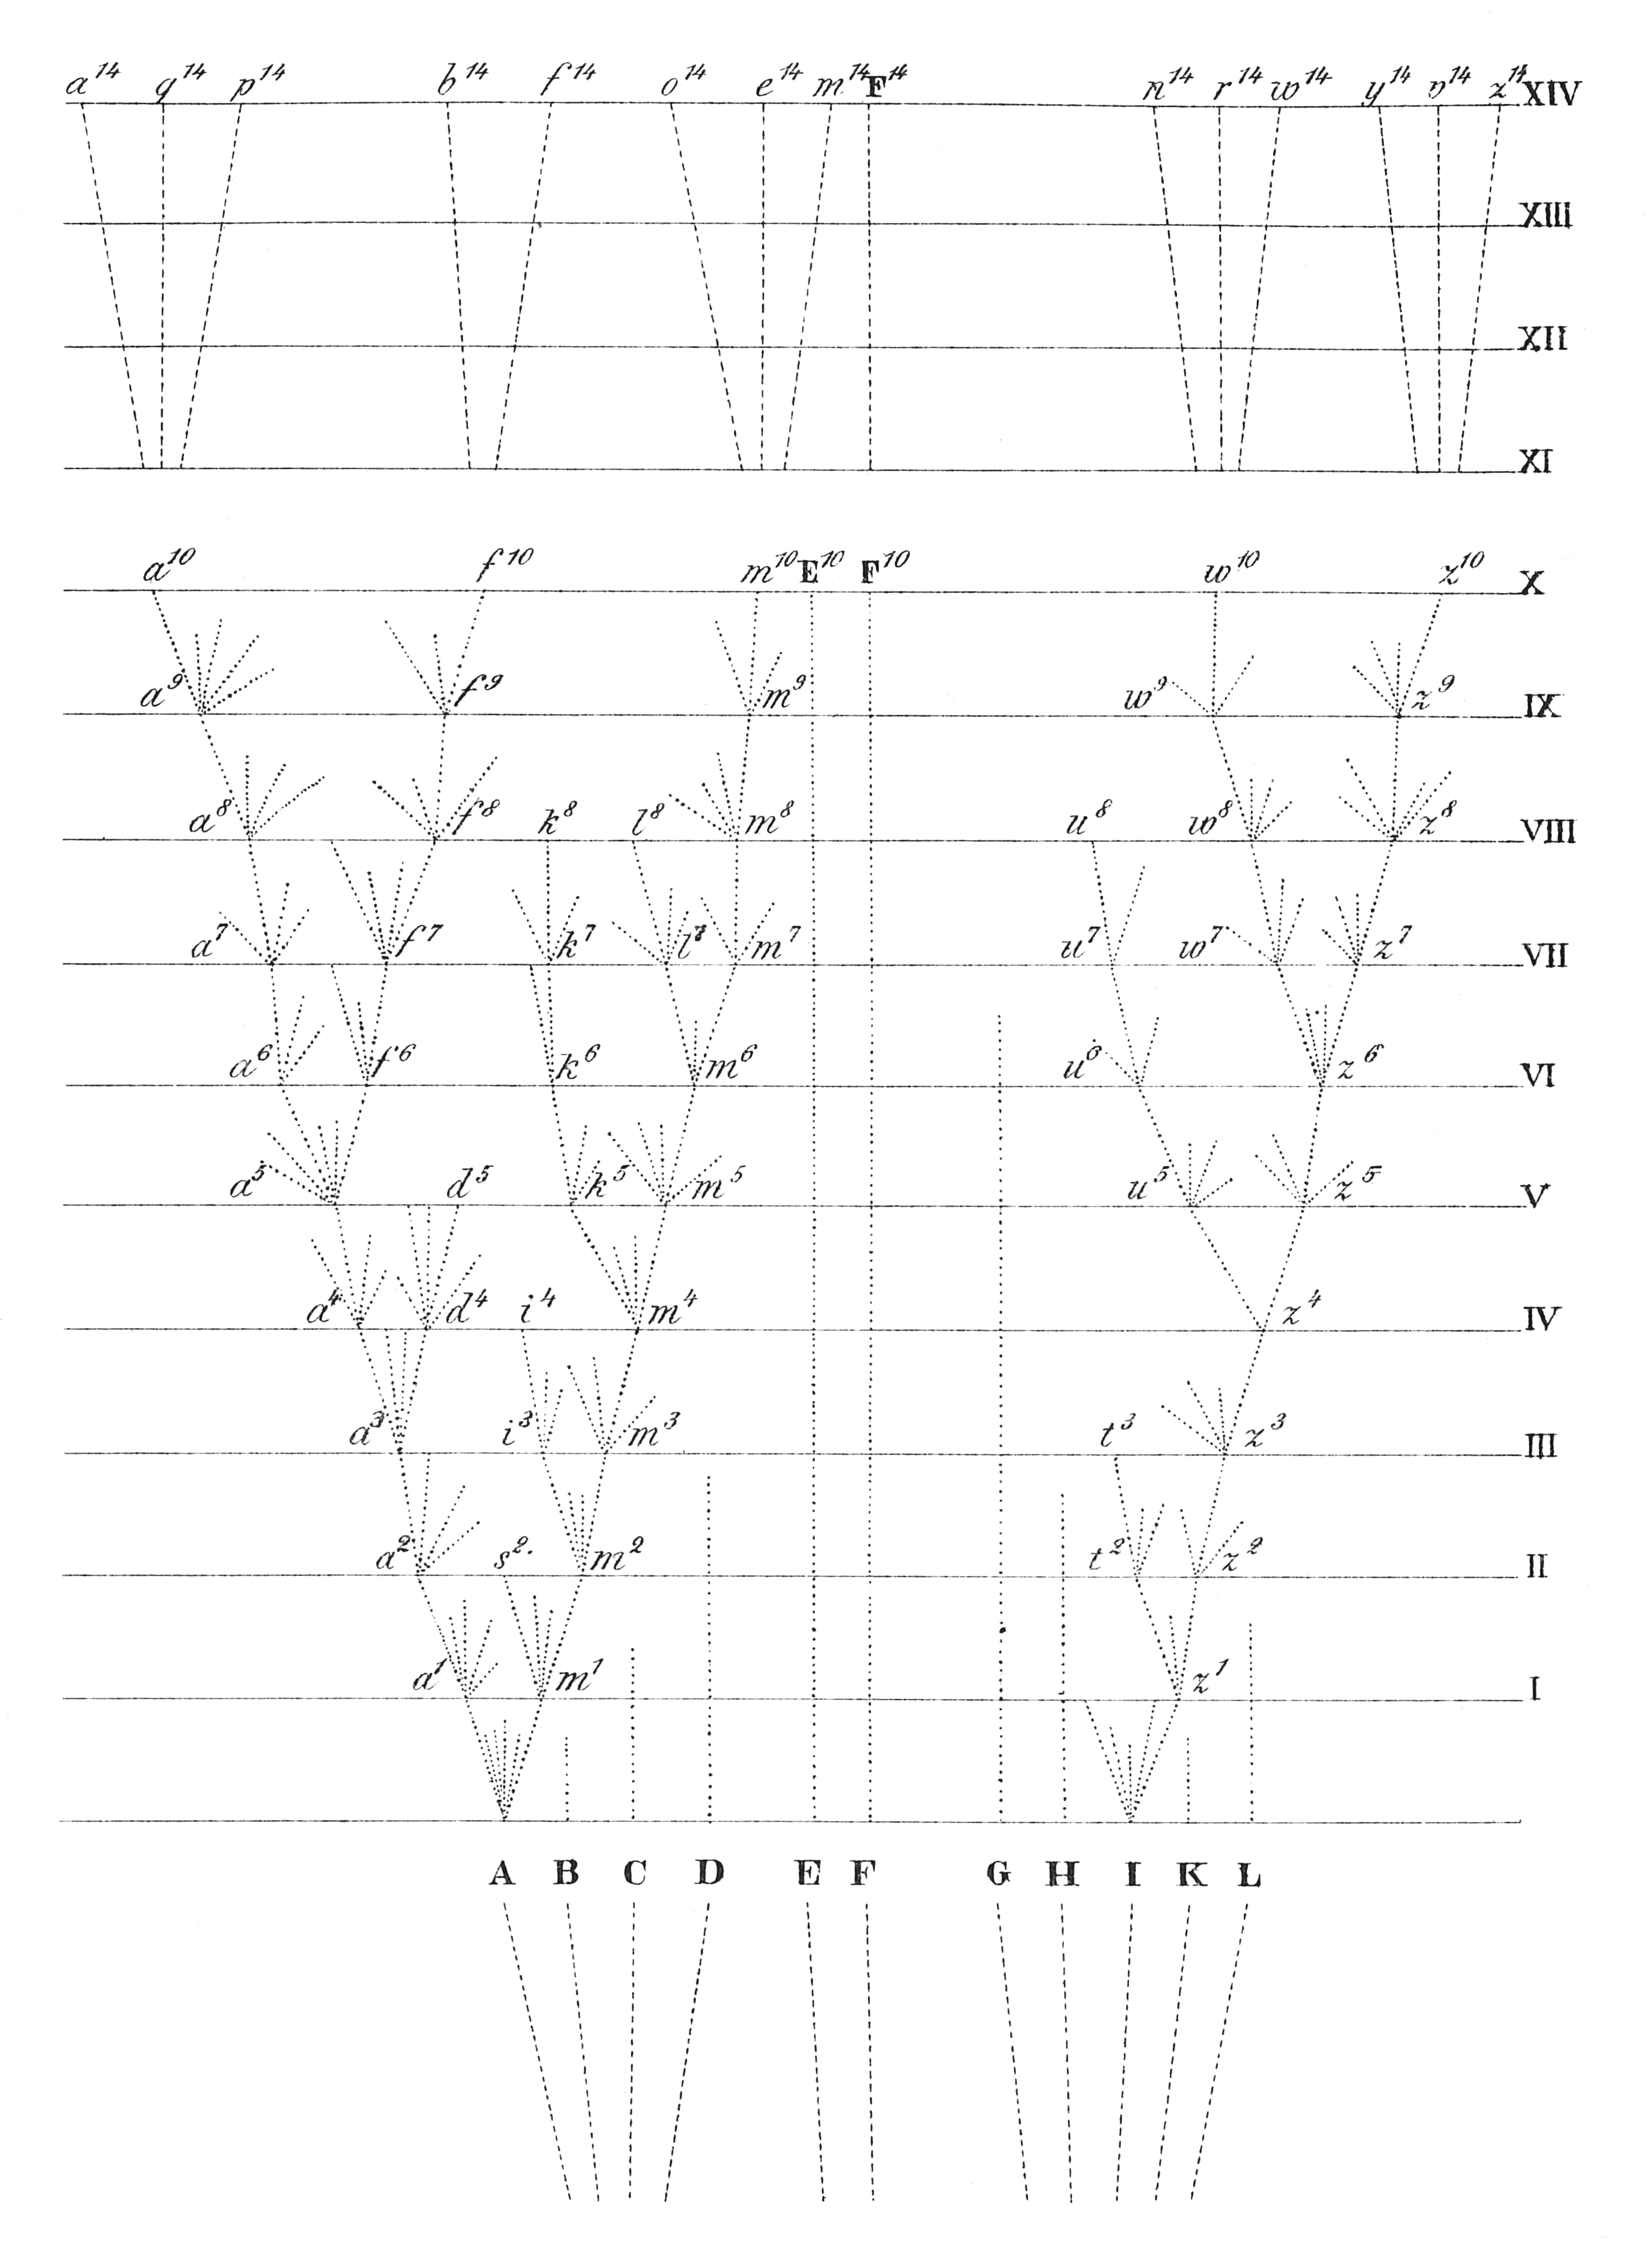
\includegraphics{bilder/plansch_1.png}
\label{fig:inverkan}
\end{figure}

framträder betydelsen af den grundsatsen, att en fördel är att härleda från karakterens divergens; ty denna skall leda dertill, att de mest skilda eller divergerande variationer (representerade af våra punkterade linier) bibehållas och ökas genom det naturliga urvalet. Då i vårt schema en af de punkterade linierna når en af de horisontala och der betecknas med en liten numererad bokstaf, så antages att variationen blifvit ökad till ett sådant omfång, att deraf bildats en distinct varietet, värd att upptagas i ett system.

Mellanrummen mellan två horisontala linier i figuren kunna motsvara 1000 generationer hvardera (bättre vore måhända tiotusen). Efter tusen generationer har arten A alstrat två väl utpräglade varieteter a${}^1$ och m${}^1$. Dessa två varieteter lefva fortfarande under samma yttre omständigheter som gjorde deras stamfäder föränderliga och benägenheten för föränderlighet är hos dem ärftlig; de skola följaktligen allt framgent vara benägna att variera och göra det också i allmänhet på ungefär samma sätt som deras stamfäder. Då dessa två varieteter vidare äro blott obetydligt modifierade former, hafva de äfven en viss böjelse att ärfva de fördelar, som gjorde deras föräldrar talrikare än de flesta andra invånare i samma trakt; de få äfven del af de mera allmänna fördelar, som gjorde det slägte hvartill stamfäderna hörde till ett i sitt eget land stort slägte. Alla dessa omständigheter äro, som vi veta, gynsamma för alstrandet af nya varieteter.

Om således dessa två varieteter äfven äro föränderliga, så skola i allmänhet de mest divergerande af deras variationer ega bestånd under de nästföljande tusen generationerna, och efter denna tids förlopp har varieteten a${}^1$ i schemat gifvit upphof till varieteten a${}^2$, hvilken enligt grundsatsen om divergensen bör visa större afvikelser från A än varieteten a${}^1$ gjorde. Vi antaga vidare att varieteten m${}^1$ har lemnat två varieteter nämligen m${}^2$ och s${}^2$, som skilja sig betydligt från hvarandra och i hög grad från det gemensamma ursprunget A. Samma process kunna vi följa steg för steg under huru lång tid som helst: några af dessa varieteter hafva efter hvarje tusental af generationer bildat en enda mer eller mindre afvikande varietet, andra två eller tre varieteter och andra åter ingen enda. Varieteterna eller de modifierade afkomlingarna som härstamma från det gemensamma ursprunget A tilltaga alltjemt i antal med divergerande karakter. I schemat är denna process fortsatt till den tiotusende generationen och i mera sammandragen och förenklad form till den fjortontusende.
Här vill jag dock anmärka, att processen icke alltid försiggår så regelbundet, som schemat föreställer, ehuru den äfven der synes något irregulier; det är sannolikt att hvarje form under lång tid blir oförändrad och sedan åter börja variera. Ej heller är det min åsigt att de mest divergenta varieteter utan undantag äro de som få väldet och föröka sig; en mellanform kan ofta ega bestånd en lång tid och stundom alstra en eller flera modifierade afkomlingar, stundom icke, ty det naturliga urvalet arbetar alltid för att fylla de platser, som antingen äro tomma eller illa besatta af andra varelser, och detta beror på oändligt invecklade förhållanden. Men såsom en allmän regel kunna vi uttala den satsen, att ju mer olika i skapnad ättlingarna af en art kunna blifva, ju flera platser i naturens hushållning äro de i stånd att intaga och i samma mån förökas deras modifierade afkomma. I vårt schema är successionslinien på regelbundna afstånd afbruten af små numererade bokstäfver, som beteckna de former hvilka varit tillräckligt skilda för att anses såsom varieteter. Men dessa afbrott äro imaginära och kunde inflätas hvar som helst på mellantider tillräckligt stora att medgifva en ansenlig grad af divergerande variation.

Då alla de modifierade ättlingarna af en gemensam, vidt utbredd art, tillhörande ett stort slägte, sträfva att få del af de fördelar som hafva gifvit deras stamfäder framgång i lifvet, skola de fortfarande tilltaga i antal och skilja sig i sina karakterer; detta betecknas i figuren genom antalet divergerande grenar utgående från A. De modifierade afkomlingarna från de sednare och mer förädlade grenarna i härstamningslinien skola sannolikt ofta intaga de tidigare och mindre förädlade grenarnas plats och således uttränga dem; detta betecknas i schemat derigenom att några af de lägre grenarna icke nå upp till de högre horisontala linierna. I några fall tviflar jag icke, att modifikationsprocessen är inskränkt till en enda härstamningsserie och att antalet ättlingar ej ökas, ehuru graden af divergens under de följande generationerna betydligt tilltagit. Detta fall skulle i schemat framställas om alla linierna, som utgå från A, vore borta med undantag af linien a${}^1$—a${}^{10}$. På sådant sätt hafva tydligen den Engelska ridhästen och den engelska rapphönshunden småningom i karakter skilt sig från sitt ursprung utan att hafva gifvit upphof till någon ny gren eller ras.

Efter tiotusen generationer antages arten A efterlemna tre former a${}^{10}$, f${}^{10}$ och m${}^{10}$, och då dessa under denna följd af generationer hafva i karakter aflägsnat sig från hvarandra, så skilja de sig nu betydligt, ehuru på olika sätt, både från hvarandra och från sitt gemensamma ursprung. Antaga vi graden af förändring emellan hvarje horisontal linie i vårt schema vara ytterligt liten, så hafva dessa former ännu blifvit blott väl markerade varieteter; men vi behöfva blott antaga dessa steg i modifikationsprocessen mera talrika eller större till omfång för att förvandla dessa tre former i tvifvelaktiga och slutligen väl bestämda arter; schemat visar således, huru små afvikelser, som utmärka varieteter, småningom steg för steg ökas till artskilnader. Om samma process fortgår under ett större antal generationer (såsom schemat visar i en sammanträngd och förenklad form), få vi åtta arter, utmärkta genom bokstäfverna a${}^{14}$—m${}^{14}$, alla härstammande från arten A. På detta sätt förökas enligt min åsigt arternas antal, och deraf bildas ett slägte.

Man kan antaga såsom sannolikt, att af ett stort slägte mer än en art varierar. I schemat har jag antagit, att en annan art I genom liknande stadier efter tiotusen generationer gifvit upphof till antingen två väl utpräglade varieteter eller två arter, alltefter den grad af förändring, som antages försiggå emellan två horisontala linier. Efter fjortontusen generationer antaga vi sex nya arter hafva bildats, betecknade med bokstäfverna n${}^{14}$—z${}^{14}$. I stora slägten är benägenheten att efterlemna ett stort antal modifierade ättlingar större hos de arter som från början äro mest skilda i karakter från hvarandra, ty dessa hafva största utsigten att fylla nya och vidt skilda platser i naturens hushållning; i schemat har jag derföre valt de långt skilda arterna A och I såsom de mest varierande och låtit dem bilda nya varieteter och arter. De andra nio arterna af vårt ursprungliga slägte, utmärkta med stora bokstäfver, kunna under en lång period efterlemna en oförändrad afkomma och detta har jag i schemat visat genom de punkterade linierna, som af brist på utrymme ej fortsatts långt uppåt.

Men under denna modifikationsprocess som schemat framställer har en annan af våra grundsatser spelat en stor rol, nämligen grundsatsen om tillintetgörelse. Då i hvarje fullt befolkad trakt det naturliga urvalet nödvändigt verkar derigenom, att de utvalda formerna hafva någon fördel öfver de andra i kampen för tillvaron, så måste de förädlade ättlingarna af en art hafva en beständig benägenhet att ersätta och undantränga sina föregångare och sina stamfäder. Ty vi få komma ihåg att kampen är i allmänhet häftigast emellan de former, som i kroppsbygnad, organisation och lefnadsvanor stå hvarandra närmast. Alla mellanformer emellan tidigare och senare stadier, det är emellan de mindre och mera förädlade stadierna af en art, likasom äfven den ursprungliga arten sjelf visa derföre i allmänhet benägenhet att dö ut. Detta är sannolikt förhållandet med många hela sidolinier, som besegras af nyare och mera förädlade linier. Likväl, om någon modifierad ättling af en art försättes i en särskild trakt eller plötsligt lämpar sig för någon viss ny station, i hvilken föräldrar och barn icke komma i någon täflan, så kunna båda fortfarande ega bestånd.

Om derföre vårt schema antages representera en hög grad af modifikation, så har arten A och alla tidigare varieteter dött ut och ersatts af åtta nya arter (a${}^{14}$—m${}^{14}$) och I har blifvit ersatt af sex (n${}^{14}$—z${}^{14}$) nya arter.

Men vi kunna gå ännu längre. De ursprungliga arterna af vårt slägte antogos likna hvarandra i olika grad, såsom förhållandet vanligen är i naturen; arten A står i närmare samband med arterna B, C och D än med de andra och arten I är närmare beslägtad med G, H, K, L än med de öfriga. Dessa två arter antogos också vara mycket allmänna och vidt utbredda, så att de ursprungligen måste hafva haft någon fördel öfver de flesta andra arterna af samma slägte. Deras modifierade ättlingar, fjorton till antal efter fjortontusen generationer hafva sannolikt ärft några af dessa företräden: de hafva också blifvit modifierade och förädlade på olika sätt i hvarje fortplantningsstadium, så att de blifvit lämpliga att innehafva många roler i deras hemlands naturhushållning. Det synes mig derföre ytterst sannolikt, att de hafva intagit just de ställen, som innehades icke blott af stamfäderna A och I utan äfven af några af de ursprungliga arterna, som närmast liknade deras stamfäder, och på detta sätt hafva de undanträngt dem. Helt få af de ursprungliga arterna skola derföre lemna efterkommande intill fjortontusende generationen, och vi kunna antaga, att blott en, F, af de två arter, som hade minsta likhet med de andra nio, ursprungliga arterna, har lemnat ättlingar ända till detta sena stadium.

De nya arter i vårt schema, som härstamma från de ursprungliga elfva arterna, äro nu femton till antal. På grund af det naturliga urvalets sträfvan att göra karaktererna divergenta är graden af karakterskilnad emellan a${}^{14}$ och z${}^{14}$ mycket större än emellan de mest skilda af de elfva ursprungliga arterna. De nya arternas förhållande till hvarandra är dessutom mycket olika. Bland de åtta ättlingarna af A är sambandet störst emellan de tre som betecknas med a${}^{14}$, q${}^{14}$ och p${}^{14}$, ty de hafva i en senare period utgrenats från a${}^{10}$; b${}^{14}$ och f${}^{14}$ äro till en viss grad skilda från de förstnämnda tre arterna, ty de hafva i en tidigare period utgått från a${}^{5}$; och o${}^{14}$, e${}^{14}$ och m${}^{14}$ stå slutligen i nära samband med hvarandra, men då de hafva afskilt sig redan vid modifikationsprocessens början äro de vidt skilda från de fem andra arterna och kunna bilda ett subgenus eller till och med ett särskildt slägte.

De sex ättlingarna af I bilda två subgenera eller genera. Men då den ursprungliga arten I är vida skild från A, ty de stå nästan vid motsatta ändar af slägtet, så bli de sex afkomlingarna af I på grund af ärftligheten allena vida skilda från de åtta afkomlingarna af A; de två grupperna antagas dessutom hafva alltjemt divergerat i skilda riktningar. Mellanformerna, som förenade de ursprungliga arterna A och I, hafva också (och detta är en mycket vigtig sak) alla med undantag af F dött ut och icke lemnat några efterkommande. De sex nya arterna som härstamma från I och de åtta som utgått från A skola derföre kunna erhålla rangen af slägten eller till och med flockar (underfamiljer).

På detta sätt hafva, som jag tror, två eller flera slägten uppkommit genom härstamning med modifikation från två eller flera arter af samma slägte, och de två eller flera urarterna kunna antagas härstamma från någon art af ett tidigare slägte. Detta är betecknadt i vårt schema derigenom att de brutna linierna under de stora bokstäfverna konvergera gruppvis nedåt emot en punkt; denna punkt representerar en enda art, den antagna stammen till våra nya subgenera och slägten.

Här kunna vi hafva god anledning att dröja ett ögonblick för att reflektera öfver karakteren af den nya arten F${}^{14}$, hvilken antages hafva divergerat blott obetydligt i karakter och bibehållit formen af F antingen oförändrad eller med blott ringa förändring. I detta fall är dess förhållande till de öfriga fjorton nya arterna af en egendomlig och invecklad beskaffenhet. Då den härstammar från en form, som stod emellan de två stamarterna A och I, hvilka antagas nu vara utdöda och okända, måste den till en viss grad i sina karakterer utgöra ett mellanstadium emellan de två grupper som utgått från dessa arter. Men då dessa två grupper hafva alltjemt i karakter skilt sig från sina urfäders typ, så är den nya arten F${}^{14}$ icke direkt en mellanform emellan dem, utan emellan typerna för tvenne grupper och hvarje naturforskare bör ej hafva svårt att påminna sig något sådant exempel.

I schemat hafva vi hittills antagit hvarje horisontal linie representera ett tusen generationer, men vi kunna lika väl låta dem föreställa millioner eller hundra millioner, och likaledes ett snitt af de på hvarandra liggande lagren af jordskorpan med de qvarlefvor af utdöda varelser de innehålla. Då vi komma till vårt kapitel om Geologien skola vi återkomma till detta ämne, och jag tror vi då skola finna, att detta schema sprider något ljus öfver de utdöda varelsernas slägtskap, hvilka, ehuru de i allmänhet tillhöra samma ordningar, familjer eller slägten som de nu lefvande, dock ofta till en viss grad i karakter stå emellan två existerande grupper; och vi kunna fatta detta förhållande, ty de utdöda arterna lefde på en mycket aflägsen tidpunkt, då ättlingarnas förgreningar ännu hade divergerat mindre från hvarandra.

Jag kan ej inse något skäl att begränsa den modifikationsprocess som vi nu genomgått till bildandet af slägten blott. Om vi i schemat antaga graden af variation, som representeras af hvarje grupp punkterade linier, vara mycket stor, bilda formerna a${}^{14}$—p${}^{14}$, b${}^{14}$—f${}^{14}$, och o${}^{14}$—m${}^{14}$ tre skilda slägten. Ifrån I hafva också utgått två skilda slägten, och då dessa senare två slägten både genom en fortsatt karaktersdivergens och genom arf från sitt ursprung skilja sig betydligt från de två slägten, som härstamma från A, så bilda de två små slägtgrupperna två skilda familjer eller till och med ordningar, alltefter graden af förändring som schemat antages föreställa. Och de två nya familjerna eller ordningarna hafva utgått från två arter af det ursprungliga slägtet och dessa två arter åter antagas härstamma från en art af ett ännu äldre okändt genus.

Vi hafva sett, att i hvarje trakt arterna af de större slägtena oftast erbjuda varieteter eller begynnande arter. Detta kunna vi i sjelfva verket vänta på förhand, ty då det naturliga urvalet verkar derigenom att en form har något företräde framför andra former i kampen för tillvaron, så verkar det hufvudsakligen på dem som redan hafva något företräde; och gruppens storlek bevisar att dess arter hafva ärft från en gemensam stamfar något gemensamt företräde. En täflan att lemna nya och modifierade ättlingar uppstår derföre emellan de större grupperna, som alla försöka att föröka sitt antal. En större grupp besegrar småningom en mindre, inskränker dess antal och förminskar på detta sätt dess utsigt till vidare variation och förädling. Inom samma stora grupp försöka de senare och mera fullkomliga undergrupperna, förgrenande sig och intagande många nya platser i naturens hushållning, att ersätta och tillintetgöra de tidigare och mindre förädlade undergrupperna; små enstaka grupper och undergrupper försvinna till slut helt och hållet. För framtiden kunna vi säga, att de grupper af organiska varelser, som nu äro stora och segerrika och äro minst afbrutna, det vill säga hafva undergått minsta förödelsen, skola under en lång tid alltjemt föröka sig. Men hvilka grupper till slut skola taga väldet, det kunna vi ej förutse, ty vi veta väl, att många grupper, som förr voro väl utvecklade, nu hafva helt och hållet gått ut. Se vi ännu längre in i framtiden, så kunna vi förutsäga, att en mängd smärre grupper skola helt och hållet utslockna och icke lemna några modifierade ättlingar på grund af de större gruppernas fortsatta och ständiga tillväxt, och att följaktligen af de arter som lefva på en viss period högst få lemna efterkommande in i en aflägsen framtid. I kapitlet om klassificering skall jag återkomma till detta ämne, jag vill blott tillägga, att med dessa satser, att ytterst få af de äldre arterna hafva efterlemnat afkomlingar och att alla ättlingarna af samma art bilda en klass, med dessa satser kunna vi lätt inse orsaken hvarföre i hvarje hufvudafdelning af växt- och djurriket blott ett ringa antal klasser finnas. Ehuru ytterst få af de äldsta arterna nu hafva lefvande och modifierade ättlingar, så måste dock jorden äfven i den mest aflägsna geologiska period hafva varit lika väl befolkad med många arter af många slägten, familjer, ordningar och klasser, som i närvarande tid.



\section{Framåtskridande i organisation.}

Det naturliga urvalet verkar såsom vi hafva sett uteslutande genom bevarande och samlande af sådana afvikelser, som kunna vara af nytta för en varelse under de organiska och oorganiska lefnadsvilkor, hvaraf den under succesiva perioder är beroende. Resultatet blir att hvarje varelse alltid sträfvar att förbättras i förhållande till dess lefnadsvilkor. Denna förbättring bör oundvikligen föra till den allmänna fulländning i organisation, som iakttages hos flertalet af de på jordytan utbredda varelserna. Här komma vi dock in på ett mycket svårt ämne, då ännu ingen naturforskare gifvit en allmänt tillfredsställande definition på hvad som förstås med organisationens fulländning. Hos ryggradsdjuren kommer härvid äfven med i räkningen deras själsförmögenheter och kroppsbygnadens större eller mindre likhet med menniskans. Man skulle tro, att graden af de förändringar, som de olika delarna och organerna undergått under sin utveckling från embryonaltillståndet intill mogen ålder, skulle kunna tjena såsom hållpunkt vid jemförelsen; dock förekomma fall, såsom vid de parasitiska krustaceerna, der flera delar af kroppen blifva ofullkomligare, så att man icke kan kalla det fullmogna djuret fullkomligare än dess larv. Von Baer’s måttstock synes ännu vara den bästa och allmännast användbara, nämligen graden af de olika delarnas differentiering (”i mogen ålder” torde väl få tilläggas) och deras speciela lämplighet för vissa förrättningar, eller fullständigheten af det fysiologiska arbetets fördelning, såsom Milne Edwards skulle säga. Huru dunkel denna sak ännu är, se vi dock om vi betrakta fiskarna till exempel, bland hvilka många naturforskare anse för de högsta dem som mest närma sig reptilierna, såsom hajarna, under det andra tillerkänna högsta platsen åt de vanliga benfiskarna (Teleostei), emedan de hafva den mest utbildade fiskformen och mest afvika från alla andra vertebrater. Ännu tydligare inse vi svårigheterna om vi vända oss till växterna, der den måttstock själsförmögenheterna kunna lemna helt och hållet bortfaller; några botanister ställa högst de växter, som i hvarje blomma hafva fullständigt utvecklade foderblad, kronblad, pistiller och ståndare, under det andra med större skäl anse för de fullkomligaste de växter, hvilkas olika organer äro starkare metamorfoserade och reducerade till mindre antal.

Taga vi de olika organernas differentiering och specialisering såsom bästa måttstocken för fullkomligheten af formernas organisation i fullväxt tillstånd (hvilket äfven innefattar hjernans fortgående utveckling för själsfunktionerna), så måste det naturliga urvalet uppenbarligen leda till fullkomlighet; ty alla fysiologer medgifva, att organernas specialisering, så vida de i detta tillstånd bättre fylla sin uppgift, är för hvarje organism en fördel, och det naturliga urvalet har således till ändamål att samla afvikelser som leda till organernas specialisering. I följd af den omständigheten, att alla organiska varelser sträfva att föröka sig i en hastigt växande progression och att intaga hvarje illa besatt plats i naturens hushållning, är det å andra sidan äfven möjligt, att det naturliga urvalet försätter en organisk varelse i sådana förhållanden, som göra många organer onyttiga eller öfverflödiga för honom och i sådant fall går han ett steg tillbaka i organisationsskalan. Om organisationen på det hela taget sedan de äldsta geologiska perioderna gått framåt ända till nu, det är en fråga, som lämpligare afhandlas i vårt kapitel om de organiska varelsernas geologiska succession.

Häremot kan man såsom invändning uppställa följande fråga: om alla organiska varelser allt ifrån början sträfvat att stiga högre och högre i utvecklingsskalan, hvaraf kommer det då, att på hela jordens yta ännu finnes en mängd de ofullkomligaste väsenden, och att i hvarje klass några former äro vida högre utvecklade än de andra? och hvarföre hafva icke dessa högre utbildade former redan öfverallt undanträngt och ersatt de mindre fullkomliga? Lamarck, som trodde på en medfödd och oundviklig benägenhet till fulländning hos alla organismer, synes hafva så väl känt vigten af denna invändning, att han ansåg sig nödgad till det antagandet, att enkla former alltjemt födas nya genom generatio spontanea (sjelfalstring). Jag behöfver icke säga, att vetenskapen på dess närvarande ståndpunkt icke lemnar något stöd för ett sådant antagande, att lefvande varelser någonstädes skulle uppstå af oorganisk materia. Enligt min teori erbjuder tillvaron af lägre organiserade djur ingen svårighet, ty det naturliga urvalet innefattar dock ingen nödvändig och allmän lag om framåtgående utveckling; det naturliga urvalet begagnar blott sådana förändringar, som för hvarje varelse äro af nytta i dess invecklade lefnadsförhållanden. Och nu kan man fråga: hvilken fördel skulle (så vidt vi kunna döma) ett infusionsdjur, en inelfsmask, eller till och med en daggmask hafva af en högre organisation? Hafva de ingen fördel deraf, så blifva de också föga eller intet fullkomligare genom det naturliga urvalet och förblifva således för oändliga tider stående på sin låga organisationsgrad. I sjelfva verket lär oss geologien, att några af de lägsta infusorier och rhizopodier sedan omätliga tider stått på samma utvecklingsgrad som nu. Det oaktadt skulle det vara förhastadt att antaga, att de flesta nu existerande lägre formerna sedan första början af sin tillvaro icke hade undergått någon förändring till fullkomlighet, ty hvarje naturforskare, som undersökt dessa organismer, hvilka nu betraktas såsom de lägsta på naturens stege, måste ofta förvåna sig öfver deras underbara och herrliga organisation.

Ungefär samma anmärkningar kunna göras med afseende på den stora olikheten i organisationsgrad inom hvarje större grupp, till exempel vid däggdjurens och fiskarnas samtidiga existens bland ryggradsdjuren, menniskans och näbbdjurets (Ornithorhynchus) bland däggdjuren, hajen och Amphioxus bland fiskarna; den sistnämde står i organernas enkelhet helt nära de ryggradslösa djuren. Men däggdjur och fiskar råka näppeligen i täflan med hvarandra; den höga ställning vissa däggdjur eller hela klasser intaga på högsta stadiet af organisation skall icke föranleda dem att intaga fiskarnas plats och på detta sätt undantränga dem. Fysiologerna tro, att hjernan måste matas med varm blod för att kunna utveckla sin högsta verksamhet och dertill är luftrespiration nödvändig, så att varmblodiga däggdjur som lefva i vatten i vissa hänseenden äro mera vanlottade än fiskarna. Likaså skola inom denna klass medlemmar af hajfamiljen sannolikt icke vara benägna att intaga Amphioxi plats, ty denna har, såsom jag hör af Fritz Müller, på södra Brasiliens magra och sandiga stränder en enda följeslagare och medtäflare, en anomalt bildad annelid. De tre lägsta däggdjursordningarna, pungdjuren, de tandlösa (trögdjuren) och gnagarna lefva i Sydamerika i samma trakter tillsammans med talrika apor och de störa hvarandra sannolikt föga. Ehuru organisationen i det stora hela kan vara stadd i framåtskridande, så måste dock utvecklingsskalan ännu framvisa alla grader, ty den höga utvecklingen hos vissa klasser eller enstaka medlemmar deraf leder ingalunda till totalt utslocknande af de grupper, med hvilka de icke komma i häftigare täflan. I några fall synas, såsom vi framdeles få se, lågt organiserade former hafva bibehållit sig ända till nu derföre att de haft egendomliga eller särskilda boningsorter, der de icke varit utsatta för någon starkare täflan, och derföre att de funnits till blott i ringa antal, hvilket enligt föregående reflexioner förminskar uppträdandet af gynsamma variationer.

Till slut tror jag, att de talrika, lågt organiserade formernas tillvaro på hela jordytan ibland nästan alla klasser beror på särskilda omständigheter. I vissa fall torde det hafva varit brist på fördelaktiga afvikelser, på hvilka det naturliga urvalet kunde hafva utöfvat sin verksamhet. I intet fall har väl tiden varit tillräcklig för att åstadkomma den högsta grad af utveckling; i några få fall kan äfven en så kallad ”organisationens återgång” hafva inträdt. Men hufvudorsaken ligger i den omständigheten, att under mycket enkla lefnadsomständigheter en högre organisation vore utan nytta, kanske till och med ofördelaktig, emedan den är finare, ömtåligare och lättare att störa och skada.

Ännu en invändning, som är rakt motsatt de nyss nämda har man framstält i följande fråga: om vi blicka tillbaka på lifvets första uppvaknande, då alla organiska varelser, såsom vi väl kunna föreställa oss, ännu egde den enklaste organisation, huru kunde då de första stegen till fulländning, differentiering och specialisering begynna? Herbert Spencer skulle sannolikt svara, att såsnart de enklaste encelliga organismer genom tillväxt och delning blifvit flercelliga eller fästat sig på någon yta, så skulle hans lag träda i verksamhet, att nämligen ”homologa enheter af hvilken ordning som helst differentieras i samma mån, som deras förhållande till på dem verkande krafter blir olika”. Men då inga fakta härvid kunna gifva oss någon ledning så är hvarje speculation i detta ämne onyttig. Det vore dock en villfarelse att antaga, att någon kamp för tillvaron och följaktligen något naturligt urval icke kunnat existera förr än många former först hade uppträdt. förändringar af en enda art på en afskild lokal kunna hafva varit fördelaktiga och genom sitt bestånd antingen omgestaltat hela arten eller gifvit upphof till två skilda former. Dock måste jag återkomma till hvad jag sagt redan vid slutet af inledningen, att ingen bör förundra sig, om ännu mycket angående arternas uppkomst måste förblifva oklart, då vi sväfva i fullkomlig ovisshet om jordinvånarnas ömsesidiga förhållande under så många förflutna perioder i deras historia.



\section{Granskning af åtskilliga invändningar.}

Jag vill nu granska några olikartade invändningar som man gjort emot mitt åskådningssätt, då några af de föregående frågorna härigenom skola blifva ytterligare belysta; att upptaga alla invändningar vore onyttigt, då sådana utgått från skriftställare, som icke gjort sig möda att riktigt förstå mina åsigter. Så har en utmärkt tysk naturforskare nyligen påstått, att den svagaste sidan af min teori ligger deri, att jag anser alla organiska varelser för ofullkomliga. Men jag har verkligen icke sagt annat, än att de alla i förhållande till de omständigheter under hvilka de lefva icke äro så fullkomliga som de kunde vara, och att detta är sant bevisa de många inhemska former, som på många delar af jorden afstå sina platser åt främmande naturaliserade inkräktare. Om också alla organiska varelser på någon tid vore fullkomligen lämpade efter sina lefnadsvilkor, så skulle de icke kunna förblifva lika fullkomliga, om dessa lefnadsvilkor långsamt ändrades; men ingen skall bestrida, att hvarje lands naturliga förhållanden liksom invånarnas antal och beskaffenhet äro underkastade ständiga vexlingar. Likaså antager en fransysk skriftställare i opposition mot hela detta arbetes anda, att enligt min åsigt stora och plötsliga förändringar träffat arterna, och frågar då triumferande, huru detta vore möjligt, då man ser att dylika modifierade former kunna kroaseras med de många oförändrade. Utan tvifvel blifva de små förändringarna eller afvikelserna beständigt störda eller tillbakahållna af kroaseringarna, med den så allmänna tillvaron af varieteter i samma land som stamarten lär, att kroasering icke nödvändigt förhindrar deras bildning, och för de vanliga lokala formerna eller geografiska raserna kan en kroasering alls icke komma i fråga. Man måste äfven komma ihåg, att affödan efter en kroasering emellan en modifierad och en icke modifierad art sträfvar att delvis ärfva båda föräldrarnas karakter och det naturliga urvalet skall helt säkert bevara till och med små tillstymmelser till nyttiga förändringar. Då dessutom en sådan kroaserad afföda har samma konstitution som den modifierade moderformen och är utsatt för samma yttre omständigheter, så skall den också lättare än andra individer af samma art undergå förändringar och modifieras på liknande sätt.

Man har framhållit, att då ingen af Egyptens kända växt- eller djurarter under de senaste tretusen åren förändrat sig, icke heller i andra verdsdelar några sådana förändringar hafva försiggått. De många djurarter, som sedan istidens begynnelse förblifvit oförändrade erbjuda en vida vigtigare invändning, ty de hafva varit utsatta för stora vexlingar i klimatet och de hafva nödgats att vandra öfver stora jordsträckor, under det i Egypten lefnadsvilkoren under de sista tretusen åren varit fullkomligt desamma. Detta från istiden lånade faktum kan väl framhållas emot dem som tro på tillvaron af en hos organismerna medfödd lag om nödvändig utveckling, men är kraftlöst emot läran om det naturliga urvalet, som blott antager, att inom en art afvikelser tillfälligtvis uppstå, och att dessa bevaras, om de äro fördelaktiga. Detta skall emellertid inträda blott efter långa tidrymder och efter förändringar i ett lands förhållanden.

Man har vidare framkastat denna fråga: då det naturliga urvalet är så verksamt, hvarpå beror det då, att icke det eller det organet i våra tider förändras och förbättras? hvarföre har icke honingbiets snabel blifvit så mycket förlängd, att biet kan suga nektar äfven i botten på rödklöfverns blommor? hvarföre har icke strutsen fått förmåga att flyga? Men antag att dessa organer hafva varierat i denna riktning, antag att trots kroasering och benägenhet till återgång tiden räckt till för det naturliga urvalets långsamma verksamhet, hvem vågar då påstå sig känna någon organisk varelses naturhistoria tillräckligt för att angifva hvilken särskild förändring skulle lända honom till nytta? Kunna vi till exempel med säkerhet säga, att en lång snabel icke skulle vara hinderlig för biet vid honingens utsugande ur så många andra blommor? Kunna vi påstå, att icke en längre snabel på grund af utvecklingens vexelverkan äfven skulle fordra en förstoring af andra mundelar, som skulle vara hinderliga vid deras fina cellbygnader? Hvad strutsen beträffar, så inses lätt, att denna öknens fågel skulle behöfva en utomordentlig tillökning i sin dagliga ranson för att kunna framforsla sin stora och tunga kropp genom luften. Så föga öfverlagda invändningar äro dock knappt värda att vederläggas.
Den utmärkta palæontologen Bronn har vid slutet af sin tyska öfversättning af detta arbete framstält den frågan, huru enligt grundsatsen om naturligt urval en varietet kan lefva jemte sin stamart. Om båda hafva blifvit lämpade för obetydligt olika lefnadsvanor eller förhållanden, kunna de existera bredvid hvarandra, ehuru bland djuren, som fritt kroaseras och drifva omkring, varieteter synas vara nästan helt och hållet inskränkta till bestämda trakter. Men om vi åsidosätta polymorfa arter, hvilkas föränderlighet synes vara af en egendomlig beskaffenhet, och alla tillfälliga variationer, sådana som olikheter i storlek, albinism etc. så finnas de mera beständiga varieteterna så vidt jag kan döma förlagda på bestämda stationer, hög- eller lågland, torra eller fuktiga områden eller skilda trakter. Bronn framhåller också, att bestämda arter aldrig skilja sig från hvarandra blott i en enda karakter utan i många delar; och han frågar efter orsaken hvarföre det naturliga urvalet ovilkorligen samtidigt inverkar på många delar af organismen. Men det finnes icke den minsta nödvändighet att tro att alla delar hafva samtidigt blifvit modifierade; de hafva kunnat förvärfvas den ena efter den andra, och då de samtidigt gå i arf, synas de oss såsom samtidigt bildade. Vexelverkan bör dessutom förklara förändringar som flera delar undergå, då en viss annan del modifieras. Bevis härpå se vi i våra husdjursarter, som om de också i en viss utvald karakter afvika betydligt, alltid till en viss grad förete afvikelser äfven i andra karakterer.

Bronn frågar vidare, huru det naturliga urvalet kan förklara olikheter emellan arter, som tyckas vara af ingen fördel för dessa arter, såsom längden af öronen eller svansen eller emaljens veck i tänderna hos flera arter af harar och råttor. Hvad växterna beträffar har detta ämne nyligen blifvit behandladt i ett utmärkt arbete af Nägeli. Han medgifver att det naturliga urvalet har gjort mycket, men han påstår, att växtfamiljerna skilja sig från hvarandra hufvudsakligen i morfologiska karakterer, som synas alldeles oväsentliga för arternas bestånd. Han tror följaktligen på en medfödd tendens till fulländning eller fortgående utveckling. Han anför cellernas anordning i väfnaderna och bladens på stammen såsom momenter på hvilka det naturliga urvalet ej kan hafva något inflytande. Dertill kan läggas de numeriska delningarna af blommans delar, fröämnenas läge, fröens form så vida den icke är af nytta vid spridningen. Professor Weismann, som granskat Nägelis afhandling, förklarar sådana olikheter med beskaffenheten af organismen under vissa omständigheters inverkan, och detta är detsamma som jag har kallat lefnadsförhållandenas direkta och bestämda verkan, hvaraf alla eller nästan alla individer af samma art variera på samma vis. Om vi påminna oss sådana fall, som vissa monstrositeter, hvilka icke kunna förklaras med regress, eller dylikt, och sådana hastiga starkt markerade bildningsafvikelser, som uppträdandet af en mossros på en vanlig ros, måste vi medgifva, att individens organisation är i stånd att enligt sina egna utvecklingslagar under vissa vilkor undergå stora modifikationer, oberoende af det gradvisa hopandet af små ärfda förändringar. Åtskilliga morfologiska olikheter till hvilka vi framdeles återkomma, höra säkerligen under denna rubrik; men många olikheter kunna i närvarande tidpunkt vara af stor nytta, eller kunna under en förfluten tid hafva varit det, ehuru vi icke äro i stånd att fatta deras bruk, och derföre hafva de stått under det naturliga urvalets inflytande. Ett ännu större antal af morfologiska skiljaktigheter kunna säkerligen betraktas såsom ett nödvändigt resultat — genom tryck, brist eller öfverflöd på näring, genom en tidigare utvecklad dels inflytande på en sedermera tillkommen, vexelverkan etc. — af andra förändringar, som alla arter måste hafva genomgått under den långa modifieringsprocessen.

Ingen vill väl påstå, att vi hittills känna bruket af hvarje del af någon växt eller funktionen af hvarje cell i ett nytt organ. För fem eller sex år sedan skulle en mängd besynnerligheter i bildningen af orchideernas blommor, stora kammar och balkar och de olika delarnas relativa läge hafva betraktats såsom onyttiga morfologiska olikheter, men nu veta vi att de äro af stor nytta och måste hafva lydt under det naturliga urvalets verksamhetsområde. Ingen kan för närvarande förklara, hvarföre bladen i en spira med hvarandra bilda vissa vinklar, men vi kunna se, att deras anordning står i sammanhang med deras afstånd från bladen på alla sidor omkring dem, och vi kunna med skäl hoppas få ett bevis, att vinklarna bero på någon sådan orsak, som tillkommandet af nya blad till den hopträngda spiran i knoppen, likasom vinklarna i biens celler ovilkorligen bero af det sätt hvarpå insekterna arbeta tillsammans.

I vissa hela grupper af växter stå fröämnena upprätta och i andra äro de hängande, och hos några få växter intaga inom samma fruktämne några frön den ena och andra den andra ställningen. Dessa lägen synas först vara rent morfologiska och icke af någon fysiologisk betydelse, men Hooker har meddelat mig, att af fröen inom samma fruktämne i några fall blott de öfre, i andra fall blott de nedre befruktas, och han förmodar, att detta sannolikt beror på den riktning i hvilken pollenröret intränger. Om detta är förhållandet, så kan fröämnenas läge, äfven om det ena är upprätt och det andra hängande, vara en följd af urval af någon ringa afvikelse i läge som kunde gynna deras befruktning och frösättning.

Flera växter, som höra till skilda ordningar, frambringa vanligen blommor af två slag, dels öppna och af vanlig skapnad, dels slutna och ofullkomliga. I de senare äro kronbladen nästan alltid reducerade till blotta rudimenter och pollenkornen äro förkrympta; i ståndarstammarna hos Ononis äro skiftevis fem ståndare rudimentära och hos några arter af Viola äro tre ståndare af denna beskaffenhet och de två öfriga behålla sin funktion, men äro mycket små. I sex bland trettio af de slutna blommorna hos en indisk viol (namnet okändt, emedan den hittills icke gifvit några fullkomliga blommor) voro foderbladen reducerade från det normala antalet fem till tre. I en grupp af Malpighiaceæ äro enligt A. de Jussieu de slutna blommorna ännu mera modifierade, ty de fem ståndare som stå midt emot foderbladen äro alla felslagna och den sjette som står emot ett kronblad är ensam utbildad; denna ståndare saknas deremot i de vanliga blommorna af dessa arter; stiftet saknas och fruktämnena äro reducerade från tre till två. I alla dessa växter äro de slutna blommorna af synnerlig nytta, ty med fullkomlig säkerhet och med en ytterst ringa mängd frömjöl lemna de en riklig mängd frön, under det de fullt utbildade blommorna tillåta tillfälliga kroaseringar med andra individer. Dessa förändringar kunna derföre vara och äro otvifvelaktigt följder af ett naturligt urval, och jag kan tillägga att nästan alla gradationer emellan fullkomliga och ofullkomliga blommor stundom kunna iakttagas hos samma växt.

Utrymmet tillåter blott några få belysningar öfver de modifikationer, som ovilkorligen följt från andra förändringar, genom brist eller öfverflöd på näring, genom tryck eller andra okända orsaker. Hos den spanska kastanien och vissa furuträd skilja sig bladens divergensvinklar enligt Schacht på de horisontala och de uppräta grenarna. Hos den vanliga vinrutan och några andra växter öppnar sig en blomma först, vanligen den centrala eller terminala, och har fem foderblad och kronblad och femrummigt fruktämne, under det de andra blommorna på växten äro fyrtaliga. Hos den britiska Adoxa har den öfversta blomman vanligen två foderflikar med de öfriga organerna fyrtaliga, under det de omgifvande blommorna hafva tre foderflikar och de öfriga blomdelarna femtaliga, och denna olikhet synes bero af det sätt, hvarpå blommorna äro packade tillsammans. Hos många Compositæ och Umbelliferæ och några andra växter hafva de periferiska blommorna sina kronor vida mera utvecklade än de centrala, och detta är sannolikt en följd af naturligt urval, ty alla blommorna blifva på detta sätt mera märkbara för de insekter som äro nyttiga eller nödvändiga till deras befruktning. I förening med blomkronans större utveckling äro reproduktionsorganerna mer eller mindre felslagna. Det är ett egendomligt förhållande att skalfrukterna vid omkretsen stundom skilja sig från dem i centrum genom form, färg och andra karakterer. Hos Carthamus och några andra Compositæ äro blott de centrala frukterna försedda med fjun, och af Hyoseris lemnar samma hufvud frukter af tre olika former. Hos vissa Umbelliferæ äro enligt Tausch de yttre frukterna orthosperma, de inre coelosperma, och denna skilnad har af de Candolle betraktats såsom af den högsta systematiska betydelse inom familjen. Om i sådana fall som föregående alla blad, blommor, frukter etc. på samma växt hade underkastats samma yttre och inre förhållanden, skulle utan tvifvel alla hafva visat samma morfologiska karakterer, och det skulle tydligen icke varit af nöden att åberopa grundsatsen om fortgående utveckling. För de små slutna blommorna, äfvensom många lägre parasitdjur, om det antages, att ett sådant biträde behöfves, måste vi åberopa en medfödd tendens till återgående utveckling.

Många exempel kunde gifvas på morfologiska karakterer som visa en höggradig föränderlighet hos växter af samma art, hvilka växa nära tillsammans, eller till och med på samma växtindivid, och några af dessa karakterer betraktas såsom systematiskt ovigtiga. Jag vill blott anföra några få fall, som jag först påträffade. Jag behöfver icke framhålla några exempel af blommor på samma stånd med dels fyrtaliga, dels femtaliga blomdelar; jag vill nämna, att enligt de Candolle blommorna af Papaver bracteatum hafva två foderblad och fyra kronblad (hvilket är vanliga förhållandet hos vallmo) eller tre foderblad och sex kronblad. Kronbladens läge i knoppen är i de flesta grupper en konstant morfologisk karakter, men professor Asa Gray försäkrar, att hos några arter af Mimulus kronbladens läge lika ofta öfverensstämmer med förhållandet hos Rhinantideæ som Antirrhineæ, till hvilken grupp slägtet hör. August S:t Hilaire anför följande fall: slägtet Xanthoxylon hör till en afdelning af Rutaceæ med enkelt fruktämne, men hos några arter finnas blommor på samma växt, till och med i samma vippa, med ett eller två fruktämnen. Hos Helianthemum har frökapseln beskrifvits såsom en- eller trerummig, och hos H. mutabile ”une lame plus ou moins large s’étend entre le pericarpe et le placenta”. Slutligen fann S:t Hilaire af Gomphia oleæformis emot sydligaste delen af dess utbredningsområde två former, hvilka han först utan betänkande antog för skilda arter, men sedan såg växa på samma buske, och han tillägger: ”Voilà donc dans un même individu des loges et un style qui se rattachent tantôt à un axe verticale et tantôt à un gynobase.”

Kan man säga om dessa växter, att de hafva blifvit påträffade under fortgåendet till en högre grad af utveckling? Tvärtom skulle jag från dessa karakterers rikliga variation sluta till, att de äro af ringa vigt för växten sjelf, huru stor betydelse de än må hafva för oss i våra klassifikationer. Ehuru vi äro fullkomligt okunniga om den verkande orsaken till hvarje modifikation, synes det likväl sannolikt af hvad vi känna om förhållandet emellan föränderligheten och förändring i lefnadsvilkoren, att under vissa förhållanden den ena bildningen haft öfvermagten öfver den andra och på detta sätt blifvit fullkomligt eller nästan konstant. Då sådana skiljaktigheter äro af ingen betydelse för artens välfärd, hafva de små afvikelser som uppkommit icke blifvit ökade eller samlade genom naturligt urval och de löpa fara att utplånas genom tillfälliga kroaseringar med andra individer. En bildning som utvecklats genom ett länge fortsatt urval blifver, då den icke längre är till någon tjenst för arten, i allmänhet föränderlig, såsom vi se förhållandet vara med de rudimentära organerna, ty den står icke längre under urvalets inflytande; men å andra sidan då i följd af organismens beskaffenhet eller förändring i de yttre förhållandena bestämda modifikationer hafva bildats, hvilka äro utan vigt för artens bestånd, kunna de öfvergå och hafva ofta öfvergått i nästan samma tillstånd till på annat sätt modifierade ättlingar. Hår hafva öfvergått på nästan alla däggdjur, fjädrar på alla fåglar och fjäll till alla reptilier. En bildning, hvilken den än må vara, som är gemensam för många beslägtade former anses af oss såsom af hög systematisk betydelse och antages på den grund ofta vara af hög fysiologisk vigt för arten. Morfologiska skiljaktigheter som vi anse för vigtiga — såsom bladens anordning, fruktämnets delning, fröämnenas läge etc. — uppträdde sannolikt först såsom vexlande variationer, som förr eller senare blefvo nästan konstanta i följd af organismens beskaffenhet eller de omgifvande förhållandena, samt genom kroasering; ty då dessa morfologiska karakterer icke hafva något inflytande på artens bestånd, så kunna små förändringar i dem icke begagnas och samlas af det naturliga urvalet. Det är ett egendomligt resultat vi sålunda kommit till, nämligen att karakterer af ringa vital betydelse för arten äro de vigtigaste för systematikern, men såsom vi skola se framdeles vid behandlingen af klassifikationens grundsatser, är denna paradox icke så stor som den först synes. Hvad man än må tänka om denna åsigt, i intet af de föregående exemplen lemna så vidt jag kan döma fakta något bevis för en medfödd tendens till fulländning eller fortgående utveckling.

Jag behöfver blott fästa mig vid två andra invändningar. Den utmärkta botanisten H. C. Watson anser mig hafva för högt uppskattat vigten af grundsatsen om karakterens divergens (på hvilken han dock uppenbart sjelf tror) och säger, att man äfven måste taga med i betraktande hvad man kunde kalla ”karakterens konvergens”. Detta är dock en allt för invecklad fråga, att vi skulle kunna inlåta oss på den här. Jag vill blott anmärka, att om två arter af två närstående slägten frambringa ett antal nya divergenta arter, kan jag väl föreställa mig, att några bland dem å ömse sidor så mycket närma sig hvarandra, att man för beqvämlighets skull kan sammanställa dem i ett intermediärt slägte, till hvilket alltså de två slägtena konvergera. Men i följd af ärftlighetsprincipens stränghet är det troligt, att dessa två grupper af nya arter åtminstone bilda två afdelningar i det nya slägtet.

Watson har äfven invändt, att det naturliga urvalets fortsatta verksamhet med karaktersdivergens slutligen måste föra till ett obegränsadt antal artformer. Hvad dock beträffar de blott oorganiska yttre lefnadsvilkoren, så är det väl sannolikt, att snart ett tillräckligt antal arter lämpar sig efter alla ansenligare olikheter i värme, fuktighet och så vidare; dock medgifver jag fullkomligt, att relationerna emellan de organiska varelserna äro vigtigare, och då arterna af de organiserade invånarna i en trakt beständigt föröka sig, så blifva äfven de organiska lefnadsvilkoren allt mera invecklade. På den grund synes det verkligen vid första påseende icke finnas någon gräns för mängden af nyttiga formolikheter och följaktligen icke för artantalet. Vi veta, att icke en gång de rikast befolkade områden på jordytan äro fullständigt försedda med arter; på Goda Hoppsudden och i Australien, som förete en förvånande mängd arter, hafva dock många europeiska arter blifvit naturaliserade. Geologien lär oss dock, att alltifrån den långa tertiärperiodens första tid antalet molluskarter icke betydligt eller alldeles icke tilltagit, liksom icke heller däggdjursarterna från mellersta tiden af samma period. Hvad är det då som förhindrar artantalets tillväxt i oändlighet? Summan af lif (jag menar icke antalet af artformer) på en gifven yta måste hafva en gräns, betingad af de fysiska förhållandena, så att om densamma är bebodd af många arter, hvarje eller i det närmaste hvarje art måste representeras af blott ett ringa antal individer och följaktligen löpa fara att tillintetgöras redan genom en tillfällig vexling i årstidernas beskaffenhet eller i antalet af fiender. En sådan förödelseprocess kan gå raskt för sig, under det arternas nybildning sker mycket långsamt. Antaga vi såsom ett fall af ytterlighet, att i England funnes lika många arter som individer, så skulle första stränga vinter eller torra sommar utrota tusen sinom tusen arter. Sällsynta arter (och hvarje art blir sällsynt, om antalet arter växer i oändlighet) lemna enligt vår ofta upprepade grundsats på en gifven tidrymd blott få fördelaktiga afvikelser och kunna således blott långsamt utveckla nya artformer. Blir en art mycket sällsynt, så måste äfven parningen emellan nära slägtingar medverka till deras undergång; åtminstone hafva några författare anfört denna omständighet såsom orsak till bisonoxens utgång i Lithauen, hjortens i Skottland, björnens i Norge och så vidare. Slutligen (och detta synes mig vara det vigtigaste), en dominerande art, som redan i sitt eget hemland öfvervunnit många medtäflare, skall alltid sträfva att vidare utbreda sig och ersätta andra. Alphonse de Candolle har visat, att de arter som sprida sig vida omkring vanligen sträfva efter mycket stor utbredning och således komma i tillfälle att på olika områden tillintetgöra mångfaldiga medtäflare och på detta sätt hindra de specifika formernas omåttliga tilltagande i verlden. Dr Hooker har nyligen visat, att på Australiens sydöstra spets, der tydligen många inkräktare från många verldstrakter finnas, de inhemska australiska arterna betydligt aftagit i antal. Jag tillåter mig icke att fråga, hvilken vigt bör läggas på alla dessa betraktelser, dock måste de i förening med hvar andra sätta en gräns för benägenheten till artformernas oändliga förökning.



\section{Sammanfattning af hela kapitlet.}

Om under den långa raden af tidsperioder och under vexlande yttre förhållanden de organiska varelserna variera i flera delar af organisationen, hvilket jag tror icke kan bestridas, om på grund af hvarje arts sträfvan att föröka sig i geometrisk progression en häftig kamp för tillvaron under någon period, årstid eller år måste utkämpas, och detta kan säkerligen icke bestridas, om vi taga i betraktande alla organiska varelsers invecklade förhållanden till hvarandra och till vilkoren för deras existens, som hafva till följd en oändlig för dem gynsam omvexling i kroppsbygnad, konstitution och lefnadsvanor, då tror jag, att det skulle synas högst egendomligt, om icke någon variation hade bildats, som varit nyttig för varelsens egen välfärd, då så många variationer förekommit som varit nyttiga för menniskor. Men om sådana för en organisk varelse gynsamma variationer förekomma, så hafva helt säkert de derigenom utmärkta individerna mesta utsigten att ega bestånd i kampen för tillvaron och enligt den stränga principen om ärftligheten sträfva de att lemna en lika utmärkt afföda. Denna grundsats om de gynsamt utrustade varelsernas bestånd har jag för korthets skull kallat det naturliga urvalet. Den leder till hvarje skapad varelses fullkomnande i förhållande till dess organiska och oorganiska lefnadsvilkor och följaktligen i de flesta fall till hvad man måste anse för organisationens fulländning; det oaktadt kunna lägre stående, enklare former länge hafva bestånd, om de äro väl lämpade för sina enklare lifsvilkor.

Enligt grundsatsen om egenskapers ärftlighet vid motsvarande ålder kan det naturliga urvalet modifiera ägget, ungen, likaväl som den fullväxta individen. Hos många djur bör det sexuela urvalet i sin verksamhet understödja det naturliga urvalet genom att tillförsäkra de starkaste och lämpligaste hannar största antalet afföda. Det sexuela urvalet kan äfven förläna sådana karakterer, som för hannarna allena äro af nytta i deras kamp med andra hannar.

Om nu det naturliga urvalet verkligen har i naturen medverkat till att modifiera och lämpa de särskilda lifsformerna efter deras olika förhållanden och lokaler, det måste bedömas efter värdet af de i de följande kapitlen gifna bevisen. Men vi se redan huru den verkar tillintetgörelse och i hvilken vidsträckt grad tillintetgörelsen varit verksam i jordens historia visar tydligt geologien. Det naturliga urvalet leder också till karakterens divergens, ty ju mer de organiska varelserna äro olika i kroppsbygnad och lefnadsvanor, ju flera kunna lefva på samma område, derpå se vi exempel om vi betrakta invånarna på en liten yta eller naturaliserade produkter. Under en arts modifikation, under alla arters oupphörliga bemödanden att föröka sitt antal, ju mera olika ättlingarna blifva, ju större är deras utsigt att segra i kampen för tillvaron. De små olikheter som utmärka varieteterna af samma art sträfva alltså ständigt att tilltaga, till dess de likna de större skilnaderna emellan arterna af samma slägte eller till och med emellan skilda slägten.

Vi hafva sett, att det är de vanliga, vidt utbredda arterna af de större slägtena som variera mest, och dessa sträfva att lemna i arf åt sina modifierade ättlingar denna öfverlägsenhet, som nu gör dem till de herskande i sina områden. Såsom vi nyss hafva anfört, leder det naturliga urvalet till karaktersdivergens och till utrotande af de mindre förädlade, intermediära lifsformerna. Från dessa grundsatser tror jag vi kunna förklara slägtskapen emellan alla organiska varelser af alla klasser på hela jordytan. Det är i sanning ett underbart faktum — ett under, som vi lätt förbise, då vi äro så förtrogna dermed — att alla djur och alla växter i alla tider och allestädes äro så beslägtade med hvarandra, att de bilda grupper, som äro subordinerade under andra grupper, så att såsom vi öfverallt finna varieteter af samma art äro mest beslägtade med hvarandra, arter af samma slägte visa mindre och olika slägtskap med hvarandra, bildande sectioner och subgenera, arter af skilda slägten äro ännu mindre beslägtade och slägtena med hvarandra stå i olika nära samband bildande underfamiljer, familjer, ordningar, underklasser och klasser. De olika underordnade grupperna i en klass kunna icke ordnas i en enkel serie utan synas snarare samla sig omkring vissa medelpunkter, och de deraf bildade grupperna åter omkring andra medelpunkter och så vidare i nästan oändliga cirklar. Från den åsigten att hvarje art blifvit särskildt skapad kan jag ej vänta någon förklaring af detta vigtiga faktum i alla organiska varelsers klassificering, men så vidt jag kan döma, kan det förklaras genom ärftlighet och genom den förenade verkan af naturligt urval, som verkar tillintetgörelse och karaktersdivergens, såsom vi i vårt schema hafva visat.

Slägtskapen emellan alla varelser af samma klass har stundom blifvit framstäld genom bilden af ett stort träd. Jag tror, att denna bild mycket nära motsvarar sanningen. De gröna och nyss utspruckna grenarna kunna föreställa nu existerande arter och de som bildats under föregående år hela raden af utdöda arter. Vid hvarje växtperiod hafva alla växande grenar försökt att förgrena sig åt alla håll och att skjuta öfver och undertrycka de omgifvande skotten och grenarna, på samma sätt som arter och artgrupper hafva försökt att i den stora kampen för tillvaron öfverväldiga andra arter. De stora grenarna, fördelade i allt mindre och mindre grenar och qvistar, voro sjelfva en gång, då trädet var litet, nyss utskjutna grenar och denna förening emellan de tidigare och de nuvarande skotten genom grenar kan väl föreställa klassifikationen af alla utdöda och lefvande arter i grupper och underordnade grupper. Af de många telningar som utvecklade sig då trädet blott var en liten buske qvarstå blott två eller tre, nu utväxta till stora grenar, och dessa bära nu alla de andra mindre grenarna: så hafva också af alla de arter, som lefvat under förgångna geologiska perioder, blott få ännu lefvande och modifierade ättlingar. Från trädets första utväxt har mången gren vissnat och fallit af och dessa förlorade grenar af olika storlek kunna representera alla de ordningar, familjer och slägten, som icke hafva några nu lefvande representanter och hvilka vi känna blott genom fossilier. Liksom vi här och der se en enstaka svag gren utgå från en gaffeldelning långt ned på trädet och genom någon lycklig slump ännu lefva qvar ända till dess spets, så se vi stundom ett djur, såsom Ornithorhynchus eller Lepidosiren, hvilket i någon ringa grad genom sina slägtskapsförhållanden förenar två större grupper, och hvilket tydligen blifvit räddadt undan en olycksbringande strid, derigenom att det bebott något skyddadt område. På samma sätt som knoppar genom tillväxt gifva upphof till nya knoppar och dessa, om de äro kraftiga, förgrena sig och på alla håll skjuta öfver mången svagare gren, så tror jag det har varit förhållandet med det stora lifsträdet, som med sina döda och afbrutna grenar fyller jordskorpan och betäcker ytan med sina herrliga alltjemt vidare fortgående förgreningar.



%FEMTE KAPITLET.





\chapter{Lagarna för variationen.}

{\it
Verkan af de yttre förhållandena. — Organernas användning och hvila i förening med naturligt urval; flyg- och synorganerna. — Acklimatisering. — Utvecklingens vexelverkan. — Utvecklingens kompensering och ekonomi. — Falsk vexelverkan. — Multipla, rudimentära och lågt organiserade bildningar äro föränderliga. — Delar, som utvecklats på ovanligt sätt, äro i hög grad föränderliga; artkarakterer mer föränderliga än slägtkarakterer; sekundära könskarakterer föränderliga. — Arter af samma slägte variera på analogt sätt. — Återgång till längesedan förlorade karakterer. Sammanfattning.
}\\[0.5cm]

Jag har hittills stundom talat om föränderlighet — så vanlig och mångfaldig hos organiska varelser under domesticering, i mindre grad i naturtillståndet — såsom om den berott på en slump. Detta är naturligtvis ett fullkomligt oriktigt uttryckssätt, som blott tjenar till att visa vår fullkomliga obekantskap med orsaken till hvarje speciel afvikelse. Några författare tro, att det tillhör de reproduktiva organernas funktioner lika mycket att frambringa individuela olikheter eller helt små bildningsafvikelser, som att göra barnet likt föräldrarna. Men den vida större föränderligheten, likasom det talrikare förekommandet af monstrositeter under domesticering än under naturtillståndet föranleder mig att tro, att sådana formafvikelser direkt bero på beskaffenheten af de lifsvilkor, under hvilka föräldrarna och deras mer aflägsna förfäder hafva lefvat under flera generationer. I första kapitlet har jag försökt att visa, att förändrade förhållanden verka på två sätt, direkt på hela organisationen eller på vissa delar allena, och indirekt genom reproduktionssystemet. I alla fall äro två faktorer verksamma, organismens beskaffenhet, som är vigtigast, och förhållandenas beskaffenhet. De förändrade förhållandenas direkta verkan leder till bestämd och obestämd modifikation. I senare fallet synes organisationen vara plastisk och vi hafva en mycket vexlande föränderlighet. I förra fallet är organismens beskaffenhet sådan, att den lätt gifver vika, så snart den utsättes för vissa omständigheter, och alla eller nästan alla individer förändras på samma sätt.

Huru stor den direkta verkan af vexlingar i klimat, föda etc., är på en organisk varelse, är ytterligt svårt att afgöra. Min tro är, att verkan är ytterligt liten på djur, men större på växter. Vi kunna åtminstone med säkerhet säga, att sådana inflytelser icke kunna hafva alstrat de många i ögonen fallande, invecklade förhållanden, som vi se öfverallt i naturen, emellan en organisk varelses kroppsbygnad och en annans. Någon ringa inflytelse kunna vi tillskrifva klimat, föda med mera: så yttrar Edward Forbes med bestämdhet att snäckor vid södra gränsen för deras utbredningsområde och i grundt vatten variera och antaga mera glänsande färger än längre norrut och på större djup, men dessa påståenden hafva sedermera betviflats. Gould tror, att fåglar af samma art äro prydda med mera lysande färger under en ständigt klar himmel, än om de lefva på öar eller vid kusterna. Wollaston är äfven öfvertygad om, att vistandet nära sjöar inverkar på insekternas färger och Moquin-Tandon meddelar en förteckning på växter, som vid sjöstränder få mer eller mindre köttiga blad, ehuru de på land ingalunda äro köttiga. Många andra sådana exempel kunde gifvas.

Det faktum, att varieteter af en art, om de komma in på området för en annan art, ofta i ringa grad antaga dennas karakterer, öfverensstämmer med vår åsigt, att arterna af alla slag blott äro väl utpräglade och permanenta varieteter. De snäckarter som äro inskränkta till de tropiska och grundare sjöarna äro i allmänhet prydda med mera lysande färger än de som blott bebo kalla och djupare sjöar. Fåglar som blott hålla sig på fastland äro enligt Gould mera bjert färgade än fåglarna på öar. Insektarter, som endast bebo sjöstränder äro, såsom hvarje samlare vet, ofta bronsfärgade och mörka; växter som uteslutande lefva vid vatten äro mycket benägna att antaga köttiga blad. Den som tror på hvarje arts särskilda skapelse måste säga till exempel, att den ena snäckan blef skapad med lysande färger för en varm sjö, men att den andra fick sin lifliga färg genom förändring då den flyttades till varmare och grundare vatten.

Om en förändring är af den ringaste fördel för en varelse, så kunna vi icke säga, huru mycket deraf bör tillskrifvas det naturliga urvalets accumulativa verkan eller de yttre lefnadsförhållandena. Så veta pelshandlare mycket väl, att djuren hafva tätare och vackrare pels, ju strängare klimatet varit under hvilket de lefvat; men hvem kan säga, i hvad mån detta beror på att de varmast klädda individerna hafva under många generationer blifvit gynnade och skyddade, eller på det stränga klimatets direkta verkan? Ty det synes väl, att klimatet har en viss direkt verkan på våra tämda fyrfotadjurs hårbeklädnad.

Exempel kunna gifvas på samma varietets uppkomst under de mest olika yttre förhållanden och å andra sidan på olika varieteters uppkomst af samma art under fullkomligt samma omständigheter. Sådana fakta visa, huru indirekt lifsvilkoren verka. Hvarje naturhistoriker känner äfven oräkneliga exempel på arter, som bibehålla sig äkta utan alla variationer, ehuru de lefva under de mest olika klimat. Sådana betraktelser föranleda mig att lägga blott ringa vigt på lifsvilkorens direkta verkan. Indirekt synas de, såsom redan är anmärkt, spela en vigtig rol genom att orsaka rubbningar i reproduktionssystemet och sålunda inleda föränderlighet, och det naturliga urvalet samlar sedan alla fördelaktiga, ehuru små variationer, till dess de blifva fullt utvecklade och för oss förnimbara.

I vidsträcktare mening kan man säga, att lefnadsförhållandena icke blott orsaka föränderlighet, utan äfven innefatta det naturliga urvalet; ty på lefnadsomständigheterna beror, om den ena eller den andra varieteten bibehålles. Men menniskans metodiska urval visar oss, att dessa två variationselementer äro väsentligt skilda; lefnadsförhållandena förorsaka föränderlighet och menniskans vilja samlar medvetet eller omedvetet förändringarna i en eller annan bestämd riktning.



\section[Verkan av ett organs bruk]{Verkan af ett organs bruk och bristande användning.}

De förhållanden vi omnämt i första kapitlet lemna föga tvifvel om att flitig användning stärker och utvidgar vissa delar hos våra husdjur, under det att samma delar försvagas, om de icke användas, och att sådana modifikationer äro ärftliga. Under fritt naturtillstånd hafva vi ingen måttstock för jemförelse att bedöma verkningarna af ett länge fortsatt bruk af vissa organer eller deras hvila, ty vi känna icke stamformerna, men många djur visa bildningar, hvilka kunna förklaras såsom följder af bristande användning. Såsom professor Owen anmärker, finnes ingen större anomali i naturen än en fågel som ej kan flyga; dock finnas flera i denna belägenhet. En sydamerikansk andart (Anas brachyptera) kan blott fladdra öfver vattenytan och har sina vingar nästan i samma tillstånd som den tama Aylesbury andrasen. Då de stora på marken betande fåglarna sällan flyga annat än för att undvika någon fara, tror jag, att de nästan vinglösa fåglar, som nu bebo eller fordom bebott öarna i oceanen, der de icke oroas af några rofdjur, hafva för sin nuvarande skapnad att tacka den omständigheten, att de icke användt sina vingar. Strutsen bebor visserligen fast land och är utsatt för faror som den ej kan undvika genom flygt, men med sina starka fötter kan den försvara sig för fienden lika väl som något af de mindre fyrfotadjuren. Vi kunna föreställa oss att strutsens stamfader hade ungefär samma vanor som trapparna och att i samma mån som det naturliga urvalet under successiva generationer förökade storleken och vigten af dess kropp, i samma mån begagnades benen mer och vingarna mindre, till dess de blefvo fullkomligt odugliga till flygt.

Kirby har anmärkt (och jag har äfven sjelf observerat samma faktum) att de främre tarserna eller fötterna på många skalbaggar som lefva i gödselhögar ofta äro afbrutna; han undersökte sjutton exemplar i sin egen samling och icke en enda hade ett spår qvar deraf. Onites apelles är så ofta i saknad af framtarserna att den beskrifves såsom saknande dem. I några andra slägten finnas de, men i mycket rudimentärt tillstånd. Hos Ateuchus, Egypternas heliga skalbagge, saknas de helt och hållet. Det är icke tillräckligt bevisadt, att tillfälliga stympningar gå i arf. Jag vill heldre förklara den totala frånvaron af främre tarser hos Ateuchus och deras rudimentära tillstånd hos några andra slägten såsom följd af bristande användning hos deras förfäder, ty då tarserna nästan alltid saknas hos många skalbaggar, som lefva i gödselhögar, måste de förloras under en tidig lefnadsperiod och kunna derföre icke vara af mycken nytta eller mycket begagnas af dessa insekter.

I några fall kunna vi lätt tillskrifva bristande användning vissa bildningsmodifikationer, som helt och hållet eller till en stor del bero på det naturliga urvalet. Wollaston har upptäckt det märkvärdiga förhållandet, att af 550 på Madeira boende skalbaggsarter 200 hafva så ofullkomliga vingar, att de ej kunna flyga, och att af tjugunio inhemska slägten icke mindre än tjugutre hafva alla sina arter i denna belägenhet! Flera sådana förhållanden, såsom att skalbaggarna i många delar af verlden af vinden drifvas ut i sjön och omkomma, att skalbaggarna på Madeira efter Wollastons iakttagelser ligga mycket dolda tills vinden är stilla och solen skiner, att antalet vinglösa skalbaggar är större på de stora öde öarna än till och med på Madeira, och särskildt det märkvärdiga faktum som Wollaston så starkt framhåller, att vissa stora grupper af skalbaggar der fullkomligt fattas, hvilka annars äro utomordentligt talrika, och hvilkas vanor nästan tvinga dem att flyga; — alla dessa betraktelser hafva kommit mig att tro, att vingarnas rudimentära tillstånd hos så många af Madeiras skalbaggar till en stor del beror på det naturliga urvalets verkningar, sannolikt i förening med bristande användning. Ty under tusentals generationer har hvarje individ, som flugit minst antingen derföre att dess vingar varit minst utvecklade eller på grund af sina lefnadsvanor, haft största utsigten att öfverlefva alla andra, emedan den icke af vinden kunnat drifvas ut i sjön, och å andra sidan hafva de skalbaggar, som gerna flögo, oftast drifvit ut i sjön och omkommit.

De insekter på Madeira, som ej lefva på marken och hvilka vanligen måste använda sina vingar för att finna sitt lifsuppehälle, såsom de af blommor lefvande skalbaggarna och fjärilarna, hafva enligt Wollastons förmenande alls icke förkrympta, utan snarare starkt utvecklade vingar. Detta står i full öfverensstämmelse med det naturliga urvalet. Ty när en ny insekt först kommer på en ö, beror det naturliga urvalets bemödande att förstora eller reducera vingarna på huruvida ett större antal individer skulle bevaras genom att lyckligt strida med vindarna eller genom att uppgifva försöket och sällan eller aldrig flyga. Förhållandet är alldeles detsamma som med matroser från ett skeppsbrutet fartyg: för de goda simmarna skulle det varit fördelaktigare, om de kunnat simma ännu längre, för de dåliga simmarna, om de alls icke kunnat simma och hållit sig vid vraket.

Mullvaden och några gräfvande gnagare hafva ögon, som äro rudimentära i storlek och i några fall fullkomligt täckta af hud och hår. Detta ögonens tillstånd är sannolikt resultatet af en småningom skeende reduktion på grund af bristande användning, men härvid spelar måhända äfven det naturliga urvalet någon rol. En Sydamerikansk gnagare, Tuco-tuco, eller Ctenomys har ännu mera underjordiska vanor än mullvaden, och en spanior, som ofta fångat sådana, försäkrade mig, att de ej sällan voro fullkomligt blinda; en som jag fick lefvande var helt säkert, såsom undersökningen tillkännagaf, blind i följd af inflammation i blinkhinnan. Då inflammationer i ögonen måste vara skadliga för djuret, och ögonen icke äro oumbärliga för ett djur med underjordiska vanor, så kan i sådant fall en förminskning af deras storlek, sammanväxning af ögonlocken och beklädnad med hår vara en ren fördel, och om detta är förhållandet, så understödes det naturliga urvalets verkan af organets bristande användning.
Det är väl bekant, att flera djur af de mest olika klasser, som bebo hålorna i Kärnthen och Kentucky, äro blinda. Hos några krabbor finnes ögonstjelken qvar, ehuru ögonen äro borta; teleskopställningen finnes qvar, ehuru teleskopet med sina glas fattas. Det är svårt att föreställa sig, att ögon ehuru onyttiga kunde vara till någon skada för djur som lefva i mörkret, och derföre tillskrifver jag deras förlust helt och hållet bristen på användning. Professor Silliman hade fångat två hålråttor (Neotoma), en blind djurart, en half engelsk mil innanför ingången till den underjordiska hålan, och således ej i dess innersta del; deras ögon voro stora och glänsande och Silliman meddelar, att sedan de under en månads tid småningom vänts vid starkt ljus, fingo de en svag synförmåga och begynte blinka.

Det är svårt att föreställa sig mera identiska lefnadsvilkor än djupa kalkstensgrottor i nästan samma klimat, så att, om man utgår från den vanliga åsigten, att blinda djur hafva blifvit särskildt skapade för Amerikas och Europas grottor, man äfven kunde vänta en stor öfverensstämmelse i organisation och slägtskapsförhållanden. Någon sådan likhet emellan de båda djurformerna förefinnes i det hela alldeles icke, och Schiödte anmärker med afseende på insekterna allena, att hela fenomenet bör betraktas såsom rent lokalt, och den likhet, som finnes emellan några invånare i Mammuthålan i Kentucky och i Kärnthenhålorna, är blott helt enkelt följd af den analogi, som öfverhufvud finnes emellan Europas och Nordamerikas fauna. Enligt min tanke måste man antaga, att amerikanska djur, som hade vanlig synförmåga, i en följd af generationer småningom från den yttre verlden trängt allt djupare och djupare in i de aflägsnaste vinklar i Kentuckyhålorna på samma sätt som europeiska djur i Kärnthenhålorna. Vi hafva några bevis för en sådan gradvis förändring af lefnadsvanorna; Schiödte anmärker: ”Vi betrakta derföre dessa underjordiska faunor såsom små ned i jorden trängande förgreningar af den närmaste omgifningens geografiskt begränsade faunor, hvilka i samma mån de tränga djupare ned i mörkret lämpa sig efter de omgifvande förhållandena; djur som föga afvika från den vanliga formen bilda öfvergången från ljus till mörker; derpå följa de djur som äro bildade för skymning och slutligen de som äro bestämda för totalt mörker, hvilkas skapnad är helt egendomlig.” Dessa Schiödtes anmärkningar hänföras icke blott till en enda, utan på helt skilda arter. Då ett djur efter otaliga generationer nått de djupaste vinklarna, har bristande användning mer eller mindre fullständigt tillintetgjort synorganet, och det naturliga urvalet har ofta åstadkommit andra förändringar, såsom en tillväxt i antennerna eller känseltrådarna till ersättning för synen. Oaktadt dessa modifikationer kunna vi ännu vänta att hos Amerikas grottdjur finna slägtskap med de andra invånarna i samma kontinent, och hos Europas grottdjur med de öfriga europeiska djuren. Detta är verkligen fallet med några af Amerikas grottdjur, såsom jag hör af Professor Dana, och några europeiska grottinsekter äro mycket nära beslägtade med den omgifvande traktens insekter. Det skulle vara mycket svårt att gifva en rationel förklaring öfver de blinda grottdjurens slägtskap med de andra invånarna i de två verldsdelarna, om man utgår från den vanliga åsigten om deras särskilda skapelse. Att några af den gamla och nya verldens grottinvånare äro nära beslägtade kunna vi vänta från den välkända slägtskapen emellan de flesta andra af deras alster. Då en blind Bathysciaart funnits i stort antal på skuggiga klippor utanför hålorna, så står sannolikt icke synens förlust hos de arter af samma slägte som bebo grottorna i något samband med boningsplatsens mörker, och det är lätt begripligt att en redan förut blind insekt lätt skall finna sig i att bebo en mörk håla. Ett annat blindt slägte, Anophthalmus, erbjuder den märkvärdiga egendomligheten, att såsom Murray anmärkte dess olika arter bo i åtskilliga hålor i Europa likaväl som i Kentuckys hålor, och att slägtet öfverhufvud blott lefver i grottor. Det är dock möjligt att stamfadern eller stamfäderna till dessa skilda slägten förut varit försedda med ögon, varit vidt utbredda i båda verldsdelarna och (liksom båda verldsdelarnas elefanter) dött ut med undantag af de i sina trånga fängelser nu lefvande arterna. Långt ifrån att öfverraskas deraf, att några af grottdjuren äro mycket anomalt bildade, såsom Agassiz anmärker om den blinda fisken Amblyopsis, och såsom förhållandet är med den blinda reptilen Proteus, jemförd med Europas öfriga reptilier, förvånas jag snarare deraf, att icke flera spillror af det gamla lifvet bevarats, då invånarna i dessa mörka boningar icke kunna hafva varit utsatta för en så särdeles sträng täflan.



\section{Acklimatisering.}

Vana är ärftlig hos växter, såsom blomningstid, nödig regnmängd för groningsprocessen, softid och så vidare och detta föranleder mig att här säga något om acklimatisering. Då det är mycket vanligt, att arter af samma slägte bebo mycket heta så väl som mycket kalla trakter, och då enligt min åsigt alla arter af samma slägte härstamma från en enda stamart, så måste, om detta är riktigt, acklimatisering utan svårighet under en lång följd af generationer kunna åstadkommas. Det är väl bekant, att hvarje art är lämpad efter klimatet i dess eget hemland: arter från en arktisk eller tempererad trakt kunna icke tåla ett tropiskt klimat och tvärtom. Många saftiga växter kunna icke uthärda ett fuktigt klimat. Men graden af arters lämplighet för det klimat under hvilket de lefva har ofta blifvit för högt uppskattad. Vi kunna sluta oss dertill af vår oförmåga att förutsäga, huruvida en importerad växt skall uthärda vårt klimat eller ej, och från det stora antalet växter och djur, som blifvit förflyttade till oss från varmare klimat och trifvas väl. Vi hafva skäl för det antagandet, att arternas utbredning i naturtillståndet begränsas lika mycket, om icke mer, af täflan med andra organiska varelser, än genom deras lämplighet för ett visst klimat. Må nu denna lämplighet i allmänhet vara noga afpassad eller icke, så hafva vi dock för några få växtarter bevis på, att de redan af naturen äro till en viss grad vända vid olika temperaturer eller acklimatiserade; arter af Pinus och Rhododendron, uppdragna af frön som Hooker samlat af träd, växande vid olika höjder på Himalaya, visa i England olika förmåga att uthärda köld. Herr Thwaites har upplyst mig om, att han observerat likartade fakta på Ceylon och liknande observationer har H. C. Watson gjort på Europeiska arter af växter, som införts från Azoriska öarna till England. Hvad djuren beträffar kunde trovärdiga fall uppgifvas af arter, som under den historiska tiden spridt sig långt omkring från varmare trakter till kallare och tvärtom; men vi veta icke bestämdt, om dessa djur voro väl afpassade efter klimatet i deras hemort, ehuru i alla vanliga fall vi antaga detta; ej heller veta vi om de sedermera blifvit acklimatiserade i sina nya hemland.

Då vi kunna antaga, att våra husdjur ursprungligen utvalts af ociviliserade menniskor derföre att de voro nyttiga och utan svårighet fortplantade sig i fångenskapen och ej derföre att de sedermera befunnos i stånd att uthärda långa förflyttningar, så tror jag att våra husdjurs allmänna och utomordentliga förmåga, att icke blott tåla vid de mest olika klimat, utan att äfven förblifva fullkomligt fruktsamma (ett mycket starkare skäl) kan tjena som argument för, att en stor del andra djur som nu äro i vildt tillstånd kunde utan svårighet bringas att uthärda vidt skilda klimat. Vi få dock icke drifva detta argument för långt, emedan några af våra husdjur sannolikt härstamma från flera vilda stammar, så att i våra tama hundraser till exempel blodet af en arktisk och en tropisk varg eller vild hund kan vara blandadt. Råttor och möss kunna icke betraktas som husdjur, men de hafva af menniskan blifvit förflyttade till många delar af verlden och hafva nu vida större utbredning än någon annan gnagare, de lefva fritt under Färöarnas kalla himmel i norden; på Falklandsöarna i söder och många öar i de heta zonerna. Derföre är jag böjd att anse lämpligheten för ett visst klimat för en egenskap, som utan svårighet kan inympas på en medfödd böjlighet i konstitution, som är gemensam för de flesta djur. Menniskans och hennes husdjurs förmåga att uthärda de mest olika klimat och sådana fakta, som att de fordna arterna af elefanten och noshörningen voro i stånd att uthärda nordens klimat, under det att de nu lefvande arterna äro tropiska eller subtropiska i sitt lefnadssätt, böra enligt denna åsigt icke betraktas såsom oregelbundenheter, utan blott såsom exempel på en mycket vanlig böjlighet i konstitution, som under vissa omständigheter gör sig gällande.

En mycket svår fråga är att afgöra huru mycket af arternas acklimatisering för ett visst klimat beror blott på vana, och huru mycket på naturens urval af varieteter med medfödd olika kroppsbeskaffenhet. Att vana och öfning derpå har ett visst inflytande, måste jag tro både från analogi och från oupphörliga varningar i arbeten öfver landthushållning, till och med i de gamla kinesiska encyklopedierna, att vara mycket försigtig vid ett djurs förflyttning från ett område till ett annat; ty det är icke sannolikt, att menniskan med så mycken framgång skulle hafva utvalt så många raser och underraser med kroppskonstitution särskildt lämpad för det af henne sjelf bebodda området: resultatet måste i min tanke tillskrifvas vanan. Å andra sidan kan jag ej se någon anledning till tvifvel, att det naturliga urvalet fortfarande sträfvar att bevara de individer som äro födda med en kroppskonstitution särdeles passande för deras hemland. I skrifter öfver åtskilliga slag af odlade växter sägas vissa varieteter bättre än andra kunna tåla vid vissa klimat: detta är på ett mycket slående sätt visadt i arbeten öfver fruktträd i Förenta Staterna, i hvilka vissa varieteter vanligen äro rekommenderade för de nordliga, andra för de sydliga staterna; och då de flesta af dessa varieteter äro nybildade, så kan man icke tillskrifva vanan deras konstitutionella olikheter. Jerusalemärtskockan, som i England aldrig fortplantar sig med frön och följaktligen aldrig lemnat nya varieteter, anföres såsom bevis att acklimatisering ej kan åstadkommas, ty den är ännu lika känslig som någonsin: den turkiska bönan har likaledes ofta blifvit framhållen i samma afsigt och med ännu mera eftertryck; men förr än någon under ett tjog generationer har sått sina bönor så tidigt, att en mycket stor del blifvit förstörd af frost, och sedan samlat frön af de få öfverlefvande, undvikande omsorgsfullt tillfälliga kroaseringar, och sedan med samma försigtighetsmått samlat frön från dessa plantor, förr kan man icke ens säga, att experimentet blifvit försökt. Och vi kunna icke heller antaga, att olikheter i konstitution icke förekomma emellan dessa plantor, ty uppgifter hafva blifvit offentliggjorda, som visa att vissa plantor synas vara vida mera resistenta än andra och jag har sjelf derpå observerat mycket slående exempel.

Öfverhufvudtaget tror jag vi kunna sluta oss till, att vana, användning och bristande öfning i vissa fall hafva spelat en ansenlig rol i modifikationen af konstitutionen och vissa organers struktur, men att verkningarna af bruk och bristande användning ofta i vidsträckt grad blifvit förenade med och stundom öfverväldigade af det naturliga urvalet.



\section{Utvecklingens vexelverkan.}

Med detta uttryck menar jag, att hela organisationens alla delar dess tillväxt och utveckling äro så nära förenade, att om små variationer uppkomma i en del och af det naturliga urvalet förökas, så förändras äfven andra delar. Detta är en mycket vigtig punkt, men ännu föga känd, och helt och hållet skilda klasser af fakta kunna här lätt förvexlas med hvarandra. Vi skola strax se att enkelt arf ofta falskeligen erbjuder utseendet af en vexelverkan. Det tydligaste exempel är, att modifikationer som samlas blott för ungens eller larvens bästa inverkar på de fullväxta individernas skapnad, på samma sätt som någon missbildning, som träffar det tidiga embryot, allvarsamt inverkar på den fullt utbildade individens organisation. De mångfaldiga delar af kroppen, som äro homologa och hvilka vid en tidig embryonal period äro identiska, synas vara benägna att variera på likartadt sätt: vi se detta deruti, att den högra och venstra sidan af kroppen förändras på samma vis, likaså framben och bakben, och vi se till och med käkarna variera på samma sätt som extremiteterna, ty några anse ju underkäken vara homolog med extremiteterna. Jag tviflar dock icke, att dessa tendenser mer eller mindre fullständigt beherskas af det naturliga urvalet; så har det en gång gifvits en hjortfamilj med blott ett horn, och om denna afvikelse hade varit af någon större nytta för afkomlingarna, är det sannolikt, att det naturliga urvalet gjort den bestående.

Såsom några författare hafva anmärkt, visa homologa delar en benägenhet att växa ihop; detta observeras ofta hos monströsa växter och ingenting är vanligare än en förening af homologa delar till en normal bildning, såsom föreningen af kronbladen i blomkronan till ett rör. Hårda delar synas inverka på formen af närliggande mjuka delar; några författare tro, att olikheten i bäckenets skapnad hos fåglar förorsakar den anmärkningsvärda skilnaden i njurarnas skapnad. Andra tro att bäckenets form hos qvinnan genom tryck inverkar på formen af barnets hufvud. Enligt Schlegel bestämmes hos ormarna läget af vissa vigtiga inelfvor af kroppens skapnad och sättet att svälja.

Beskaffenheten af detta sammanhang är ofta mycket dunkel. Isidore Geoffroy S:t Hilaire har med eftertryck framhållit, att vissa missbildningar mycket ofta förekomma tillsammans, andra sällan, och detta utan att vi äro i stånd att angifva något skäl dertill. Hvad kan vara mer egendomligt än sambandet emellan blå ögon och fullkomlig döfhet hos katten, färgen på sköldpaddhonans skal och hennes kön, fjäderbeklädnaden på fötterna och huden emellan de yttre tårna hos dufvorna eller emellan närvaron af mer eller mindre dun hos de unga nykläckta fåglarna och deras framtida fjäderbeklädnads färg, eller åter förhållandet emellan håret och tänderna hos den nakna turkiska hunden, ehuru här otvifvelaktigt homologi kommer med i spelet. Med afseende på detta slag af vexelverkan synes det mig knappt såsom en tillfällighet, att de två däggdjursordningar hvilka mest afvika i sin hudbeklädnad, nämligen Cetacea (hvalar) och Edentata (tandlöse, bältor, myrkottar), också äro de mest afvikande i sin tandbygnad.

Jag känner intet fall, som vore lämpligare att visa vigten af lagarna för vexelverkan, oberoende af fördel och således äfven af det naturliga urvalet, än skilnaden emellan de yttre och inre blommorna hos vissa växter af familjerna Compositæ och Umbelliferæ. Hvar och en känner skilnaden emellan kantblommorna och de centrala blommorna hos till exempel tusenskön (Bellis) och denna skilnad är ofta åtföljd af förkrympning af vissa blomdelar. Men hos vissa Compositæ skilja sig äfven frukterna i storlek och skapnad och till och med fruktämnet med dess bidelar visar olikheter såsom Cassini har beskrifvit. Dessa skilnader hafva af några författare blifvit tillskrifna tryck och skapnaden af strålblommornas frukter hos några Compositæ understödja denna åsigt. Men bland umbellaterna är det, såsom Hooker upplyser mig, ingalunda hos de tätaste blomhufvuden, som de inre och yttre blommorna oftast visa skiljaktigheter. Man kunde tro, att utvecklingen af de i blomflockens rand befintliga kronbladen skulle beröfva vissa andra blomdelar deras näring och sålunda förorsaka deras förkrympning, men i vissa Compositæ finnas olikheter i frukterna af de yttre blommorna, utan någon skilnad i blomkronan. Möjligt är, att dessa olikheter kunna stå i sammanhang med ett olika tillflöde af näringsvätska till de yttre blommorna: vi veta åtminstone, att af oregelbundna blommor de som stå närmast axeln oftast visa benägenhet att blifva regelbundna. Såsom ett exempel härpå och tillika såsom ett slående fall af vexelverkan, vill jag tillägga att jag nyligen i några trädgårdspelargonier observerat, att centralblomman i knippet ofta förlorar de mörka fläckarna på de öfre kronbladen, och att om detta händer det vidhängande honingsgömmet försvinner; om färgen är borta blott från det ena af de två öfre kronbladen, är honingsgömmet blott mycket förkortadt.

Med afseende på olikheterna i blomkronan af de yttre och centrala blommorna af ett blomhufvud eller en blomflock, vill jag nämna, att jag alls icke anser Sprengels åsigt vara så sökt, som den först synes, att kantblommorna tjena till att ditlocka insekter, hvilkas verksamhet är särdeles vigtig för befruktningen af dessa två familjers växter: och om det är af nytta, kommer väl äfven det naturliga urvalet med i spelet. Deremot synes det knappt möjligt att skilnaden emellan både den inre och yttre skapnaden af fröen som icke alltid är förenad med olikheter i blommorna, kan vara af någon fördel för växten; dock äro dessa olikheter hos Umbelliferæ af så synbar vigt, att den äldre de Candolle grundade sina stora indelningar af denna familj på sådana olikheter. Vi se sålunda att modifikationer, som af systematikern betraktas såsom af högt värde, kunna helt och hållet bero på okända lagar för utvecklingens vexelverkan och ej erbjuda arterna, så vidt vi kunna se, den ringaste fördel.

Vi kunna ofta oriktigt tillskrifva utvecklingens vexelverkan bildningar, som äro gemensamma för hela artgrupper och hvilka i sjelfva verket blott bero på ärftlighet; ty en gammal stamfader kan genom naturligt urval hafva förvärfvat någon egendomlighet i kroppsbildning och efter tusen generationer någon annan, helt och hållet oberoende förändring och dessa två förändringar, som sedan gått i arf till en hel grupp af ättlingar med skilda lefnadsvanor, kunna helt naturligt anses stå i något nödvändigt samband med hvarandra. Så tviflar jag icke heller derpå, att vissa skenbara vexelverkningar, som möta genom hela ordningar, blott och bart bero på det sätt, hvarpå det naturliga urvalet kan verka. Alphonse de Candolle har till exempel anmärkt, att vingade frön aldrig förekomma i frukter som icke öppnas; jag skulle förklara denna regel så, att fröen icke kunna småningom antaga vingar genom det naturliga urvalet annat än i öppnade frukter, så att växtindivider med frön, som voro blott litet bättre egnade att föras vida omkring, kunde få någon fördel öfver andra, som lemna frön mindre tjenliga att spridas, och denna process kan omöjligen försiggå i en frukt som icke öppnar sig.



\section{Utvecklingens kompensering och ekonomi.}

Den äldre Geoffroy och Goethe uppstälde ungefär samtidigt sin lag om utvecklingens kompensering eller jemvigt, eller såsom Goethe uttryckte den, ”för att slösa på ena sidan måste naturen hushålla på den andra”. Till en viss grad passar detta i min tanke in på våra kulturalster: om näring tillflödar en del eller ett organ i öfvermått, så strömmar den sparsamt eller åtminstone icke i öfverflöd till en annan del; det är derföre svårt, att få en ko att gifva mycket mjölk och på samma gång blifva fet. Samma kålvarietet kan icke lemna en riklig mängd födande blad och en stor mängd oljrika frön. Då fröen i våra frukter förkrympa, vinner frukten sjelf i storlek och beskaffenhet. Hos våra höns åtföljes vanligen en stor fjädertofs på hufvudet af en förminskad kam och ett stort skägg af förminskade köttflikar. Dock kan man näppeligen antaga, att denna lag eger i full utsträckning sin tillämpning på arter i naturtillståndet, ehuru många goda iakttagare, isynnerhet botanister, tro på dess sanning. Här vill jag dock ej anföra några exempel, ty jag kan svårligen finna ett medel att skilja emellan följderna af å ena sidan en dels stora utveckling genom det naturliga urvalet och de närliggande delarnas förkrympning af samma orsak eller af bristande användning, och å andra sidan ett organs förkrympning genom brist på näringsämnen i följd af andra närliggande delars utomordentliga utvidgning.

Jag förmodar också, att några anförda fall af kompensering kunna jemte några andra fakta bringas under en mera allmän grundsats, att nämligen det naturliga urvalet alltjemt försöker att vara sparsamt i hvarje del af organisationen. Om under förändrade lefnadsvilkor ett förut fördelaktigt organ blifver mindre nyttigt, så företages väl en förminskning, ehuru ringa, i dess utveckling af det naturliga urvalet, ty det skulle icke vara gynsamt för individen att förslösa sin näring på att uppbygga ett onyttigt organ. Blott på detta sätt kan jag förstå ett faktum, som mycket förvånade mig, då jag undersökte cirripederna, och många exempel kunde gifvas derpå, nämligen att en cirriped, som lefver såsom parasit inuti ett annat djur och på detta sätt är skyddad, förlorar mer eller mindre fullständigt sitt eget skal. Detta är fallet med hannen af Ibla och på ett i sanning utomordentligt sätt med Proteolepas; alla andra cirripeders pansar består af de tre ofantligt utvecklade främre segmenterna af hufvudet och är försedt med starka nerver och muskler, men hos den parasitiska och skyddade Proteolepas är hela främre delen af hufvudet reducerad till ett blott rudiment fästadt vid basen af gripantennerna. Inbesparandet af ett stort och inveckladt organ, som blifvit öfverflödigt genom Proteolepas’ parasitiska lefnadssätt, om det också skedde blott småningom, skulle vara en afgjord fördel för hvarje efterkommande individ af arten; ty under den kamp för sin tillvaro, som hvarje djur måste utkämpa, skulle hvarje proteolepasindivid hafva bättre utsigt att försvara sig, om en mindre mängd näring bortslösades till utbildande af ett numera fullkomligt onyttigt organ.

På detta sätt tror jag det alltid lyckas för det naturliga urvalet i längden att reducera och inbespara hvarje del af organisationen, så snart den blifvit öfverflödig, utan att derföre på något sätt gifva anledning till en annan dels större utveckling i motsvarande grad. Och tvärtom lyckas det lika väl för det naturliga urvalet att bringa ett visst organ till stor utveckling utan att dertill såsom en nödvändig kompensering behöfva reduktionen af några närliggande delar.



\section[Rudimentära bildningar]{Multipa, rudimentära och lågt organiserade bildningar
äro föränderliga.}

Såsom Isidore Geoffroy S:t Hilaire anmärker, synes det vara en regel både ibland varieteter och arter, att om en del eller ett organ förekommer i mångfaldigt antal hos samma individ (såsom kotorna hos ormarna och ståndarna hos polyandriska blommor) antalet är föränderligt, hvaremot, om antalet är mindre, det är mera konstant. Samma författare och några botanister hafva äfven anmärkt, att mångtaliga organer äro mycket benägna för föränderlighet i sin inre bygnad. Så vida denna ”vegetativa upprepning”, för att begagna prof. Owens uttryck, är ett tecken till låg organisation, synes ofvanstående iakttagelse stå i sammanhang med den bland naturforskarna mycket allmänna åsigten, att varelser som stå lågt på naturens skala äro mera föränderliga än de högre. Med låg organisation menar jag i detta fall, att de olika delarna af organisationen äro blott i ringa mån specielt utbildade för vissa förrättningar; så länge samma del har att fullborda olikartade värf, kunna vi måhända inse, hvarföre den skulle förblifva föränderlig, det vill säga, hvarföre det naturliga urvalet icke med samma omsorg skulle hafva bevarat eller förkastat hvarje liten formafvikelse, som om organet vore bildadt blott för ett särskildt ändamål. En knif, som är ämnad att skära hvad som helst, kan hafva nästan hvarje godtycklig form, då deremot ett verktyg för ett visst ändamål lämpligare har en viss bestämd form. Vi få aldrig glömma, att det naturliga urvalet verkar på hvarje varelses särskilda organer blott i och för individens nytta.

Ofullkomligt utvecklade, rudimentära organer äro också i hög grad benägna för föränderlighet, såsom vissa författare påstå, i min tanke med fullt skäl. Vi skola återkomma till de rudimentära och abortiva organerna i allmänhet och här vill jag blott tillägga, att deras föränderlighet synes bero på deras gagnlöshet, och på den grund har det naturliga urvalet ingen förmåga att förhindra afvikelser i deras bygnad. Rudimentära organer äro således prisgifna åt det fria inflytandet af utvecklingens olika lagar, följderna af en länge fortsatt overksamhet och benägenheten till återgång.



\section[Variation i ovanliga grader]{En hos en art i ovanlig grad eller på ovanligt sätt
utvecklad del har i jemförelse med samma del
hos en beslägtad art en stor benägenhet att
variera.}

För många år sedan öfverraskades jag högeligen af ett likartadt yttrande af Waterhouse; en observation af prof. Owen öfver armarnas längd hos orang-outang gör det sannolikt, att äfven han har kommit till nästan samma åsigt. Jag kan icke hoppas öfvertyga någon om riktigheten af detta påstående utan att framlägga den långa lista af fakta som jag samlat, men som ej här kan införas. Jag kan blott uttala min öfvertygelse, att denna regel är mycket allmän. Flera källor till fel har jag visserligen blifvit varse, men jag tror mig hafva fästat tillbörligt afseende vid dem. Framför allt är att observera, att denna regel icke har sin tillämpning på någon del, om den ock är ovanligt utvecklad, med mindre dess utveckling är ovanlig i jemförelse med samma del hos närbeslägtade arter. Flädermössens vingar äro visserligen en ytterst abnorm bildning hos däggdjursklassen, men här har regeln ingen tillämpning, då vingbildningen tillhör en hel större grupp; den kunde blott tillämpas, om någon art af flädermöss hade sina vingar utbildade på ett ovanligt sätt i jemförelse med de andra arterna af samma slägte. Regeln har en mycket sträng tillämpning på ”sekundära sexualkarakterer” om de äro ovanligt utbildade. Med termen ”sekundära sexualkarakter” menar Hunter sådana karakterer som tillhöra ett enda kön, hanne eller hona, utan att stå i omedelbart sammanhang med fortplantningen. Regeln gäller både hannar och honor, men då honorna mera sällan erbjuda anmärkningsvärda sekundära sexualkarakterer, så kan regeln mera sällan tillämpas på dem. Att regeln är så fullständigt användbar på dessa karakterer, beror väl på deras stora föränderlighet, vare sig de äro ovanligt utbildade eller icke, ett förhållande hvarom föga tvifvel kan hysas. Men att vår regel icke är inskränkt härtill visa de hermafroditiska cirripederna, och jag vill tillägga, att jag vid undersökningen af denna ordning lade särskildt märke till Waterhouses yttrande, och jag är fullkomligt öfvertygad att regeln nästan oföränderligen gäller hos cirripederna. I ett kommande arbete skall jag gifva en lista på mera anmärkningsvärda fall, här vill jag blott i korthet gifva ett, som belyser regeln i dess vidsträcktaste användning. Täckvalvlerna hos de sessila cirripederna (Balanider) äro i hvarje mening mycket vigtiga organer och skilja sig ytterst litet hos skilda slägten; men hos flera arter af ett slägte, Pyrgoma, visa dessa valvler en märkvärdig grad af olikhet: de homologa valvlerna äro hos skilda arter stundom fullkomligt olika formade; och graden af afvikelse hos individerna af flera arter är så stor, att det icke är någon öfverdrift att påstå, att varieteterna skilja sig mera från hvarandra i karakteren af dessa vigtiga valvler, än andra arter af skilda slägten.

Då fåglar inom samma trakt variera utomordentligt litet, har jag fästat särskild uppmärksamhet vid dem och regeln synes mig helt visst hafva stor giltighet hos denna klass. Jag kan icke visa, att den har tillämpning på växterna och detta skulle allvarsamt hafva skakat min tro på dess sanning, om icke växternas stora föränderlighet öfverhufvud hade gjort det särdeles svårt att jemföra den relativa föränderlighetsgraden.
Om vi hos en art se en del eller ett organ utveckladt på anmärkningsvärdt sätt eller i ovanlig grad, så ligger det nära till hands att antaga, att organet är af stor vigt för denna art, och dock är delen i detta fall utomordentligt benägen för föränderlighet. Hvarpå kan detta bero? Från den åsigten, att hvarje art blifvit särskildt skapad med alla sina delar sådana dessa äro, kan jag icke se någon förklaring. Men vår åsigt, att grupper af arter hafva härstammat från andra arter och hafva blifvit modifierade af det naturliga urvalet, tror jag kan sprida något ljus häröfver. Om hos våra husdjur någon del eller hela djuret försummas och något urval ej användes, så skall en sådan del (såsom kammen hos Dorkinghönsen) eller hela rasen upphöra att bevara sin nästan likformiga karakter. Rasen säges då hafva urartat. I rudimentära organer och sådana, som blott i ringa grad blifvit specielt bildade för ett visst ändamål och måhända äfven i polymorfa grupper se vi ett nästan liknande fall i naturen, ty i sådana fall har det naturliga urvalet icke kunnat komma i full verksamhet och således lemnas organisationen i en vacklande ställning. Men hvad som häraf mera särskildt angår oss är, att hos våra husdjur de delar, som för närvarande undergå hastiga förändringar genom ett fortsatt urval, också äro i hög grad benägna att variera. Man må betrakta de olika dufraserna, se denna märkvärdiga olikhet i näbben hos de olika tumletterna, i näbben och hudvårtorna hos brefdufvorna, i påfågeldufvornas hållning och stjert, etc., och dessa äro de karakterer vid hvilka de engelska amatörerna hufvudsakligen fästa afseende. Äfven underraserna, såsom den korthöfdade tumletten, äro svåra att få fullkomliga och ofta födas individer som vidt skilja sig från typen. Man kan derföre i sanning säga att en beständig strid fortgår emellan å ena sidan så väl benägenheten för återgång till ett mindre modifieradt stadium som en medfödd sträfvan till vidare föränderlighet af alla slag, och å andra sidan inflytandet af fortfarande urval till att bibehålla rasen ren. I längden vinner urvalet seger och vi frukta icke att få en vanlig tumlett af en ädel korthöfdad ras. Men så länge urvalet fortgår hastigt, kunna vi vänta att finna mycken obeständighet hos de organer som undergå modifikationer. Det förtjenar vidare att anmärkas, att dessa föränderliga karakterer, som menniskan med sitt urval framkallar, stundom af fullkomligt okända orsaker mera hålla sig till ena könet än det andra, i allmänhet till hannarna, såsom brefdufvans hudvårtor och kroppdufvans utvidgade kräfva.
Låt oss nu återvända till naturen. Om ett organ har blifvit utveckladt på något utomordentligt sätt hos någon art, jemförd med andra arter af samma slägte, kunna vi antaga, att detta organ har undergått en ansenlig förändring sedan den tid, då arten afskilde sig från slägtets gemensamma stamfader. Denna period ligger sällan ytterligt långt tillbaka, då arter i allmänhet ej bibehålla sig längre än under en geologisk period. En utomordentlig grad af modifikation förutsätter en ovanligt stor och länge fortsatt föränderlighet, som det naturliga urvalet länge användt till artens bästa. Men då det ovanligt utbildade organets föränderlighet har varit så stor och länge fortfarit under en ej så ytterligt aflägsen period, kunna vi såsom en allmän regel vänta att ännu finna en större föränderlighet i sådana delar än i andra delar af organisationen, hvilka under en mycket längre period hållit sig beständiga. Och detta är enligt min öfvertygelse verkliga förhållandet. Att striden emellan det naturliga urvalet å ena sidan och benägenheten till återgång och föränderligheten å den andra under tidens lopp skall upphöra och att äfven de mest abnormt bildade organer kunna blifva beständiga, derpå ser jag intet skäl att tvifla. Om derföre ett organ, huru abnormt det än är, har i ungefär samma tillstånd öfvergått på många modifierade ättlingar, såsom flädermössens vingar, måste det enligt min teori hafva funnits redan under en ofantligt lång period i nästan samma tillstånd, och derföre är det nu icke mera föränderligt än något annat organ. Det är blott i de fall, i hvilka modifikationen är jemförelsevis ny och utomordentligt stor, som vi skola i hög grad ännu finna denna generativa föränderlighet, som vi kunna kalla den. Ty i dessa fall skall föränderligheten blott sällan ännu hafva blifvit tillintetgjord genom ett fortsatt urval af de individer som varierade på lämpligt sätt och i lämplig grad, och genom ett fortsatt afskiljande af dem som sträfvade att återgå till en tidigare och mindre modifierad form.



\section[Artkaraktarer äro föränderligare]{Artkarakterer äro föränderligare än slägtkarakterer.}

Den grundsats, som innefattas i denna tankegång, kan vidare utsträckas, ty det är bekant att artkarakterer äro föränderligare än slägtkarakterer; ett enkelt exempel förklarar hvad jag härmed menar. Om några arter i ett stort växtslägte hafva blå blommor och andra röda, så är blommornas färg blott en artkarakter och ingen skulle öfverraskas deraf att någon af de blå arterna varierade med röda blommor eller tvärtom, men om alla arterna hade blå blommor, då vore färgen en slägtkarakter och dess föränderlighet vore en mera ovanlig omständighet. Jag har valt detta exempel, emedan derpå icke kan tillämpas den förklaring som de flesta vetenskapsmän eljest pläga framhålla, att nämligen specifika karakterer äro mera föränderliga än slägtkarakterer, emedan de hemtas från delar af mindre fysiologisk vigt än de delar, som vanligen begagnas att klassificera slägtena. Jag tror visserligen att denna förklaring delvis, ehuru blott indirekt, är riktig, jag skall likväl återkomma härtill i vårt kapitel om klassifikationen. Det torde vara nästan öfverflödigt att anföra exempel till bevis för ofvanstående sats, att artkarakterer äro mera föränderliga än slägtkarakterer; men jag har upprepade gånger i naturhistoriska verk funnit, att om någon författare med öfverraskning iakttagit att ett vigtigt organ, som i allmänhet i stora artgrupper är mycket konstant, hos närbeslägtade arter visade betydliga skiljaktigheter så var det också föränderligt hos individerna bland några af dessa arter. Och detta förhållande visar, att en karakter, som i allmänhet har värdet af slägtkarakter, om den faller i värde och blir blott af en artkarakters värde, ofta blifver föränderlig, ehuru dess fysiologiska vigt förblir densamma. Något likartadt äger rum vid monstrositeter: åtminstone tyckes Isidore Geoffroy S:t Hilaire icke tvifla på, att ju större olikheter ett organ visar i skilda arter af samma grupp, ju mera är det underkastadt individuela anomalier.

Enligt den vanliga åsigten, att hvarje art är en oberoende skapelse, huru skulle den del af organisationen, som skiljer sig från samma del hos andra särskildt skapade arter af samma slägte, kunna vara mera föränderlig än de delar som äro nästan öfverensstämmande hos skilda arter? Jag kan icke deraf finna någon förklaring häröfver. Men om vi utgå från den åsigten, att arter äro blott väl utpräglade och permanenta varieteter, kunna vi med all säkerhet vänta att finna dem fortfarande variera i de delar af organisationen, hvilka inom en relativt ny period hafva varierat och på detta sätt kommit att förete afvikelser. Eller för att framställa förhållandet i andra ord: — de kännetecken, hvaruti alla arter af ett slägte likna hvarandra, och hvaruti de skilja sig från arterna af något annat slägte, kallas slägtkarakterer, och dessa karakterer tillskrifver jag i allmänhet arf från någon gemensam stamfader; ty det bör väl sällan hafva händt, att det naturliga urvalet på fullkomligt samma vis modifierat flera arter, lämpade för mer eller mindre olika lefnadsvanor: och då dessa så kallade slägtkarakterer hafva gått i arf från en aflägsen tid, då arterna först afskilde sig från deras gemensamma ursprung och följaktligen icke hafva varierat något eller blott obetydligt, är det icke sannolikt att de skulle variera för det närvarande. Å andra sidan, de kännetecken som skilja arterna af samma slägte från hvarandra kallas artkarakterer, och då dessa sedan den tid då de afskilde sig från sin gemensamma stamfar hafva varierat, så är det sannolikt, att de ofta ännu skola till en viss grad vara föränderliga, åtminstone mera föränderliga än de delar af organisationen, som en längre tid förblifvit konstanta.



\section[Sekundära sexualkarakterier]{Sekundära sexualkarakterer äro mer föränderliga
än artkarakterer.}

I sammanhang med detta ämne vill jag göra blott två andra anmärkningar. Jag tror man skall medgifva, utan att jag ingår i några detaljer, att sekundära sexualkarakterer äro mycket föränderliga; jag tror också man skall medgifva, att arter af samma grupp skilja sig från hvarandra vida mer i sina sekundära sexualkarakterer än i andra delar af sin organisation; jemför man till exempel graden af olikhet emellan hannarna af hönsfåglarna, hos hvilka de sekundära könskaraktererna äro starkt utvecklade, med graden af olikhet emellan deras honor, så inses lätt sanningen af detta påstående. Orsaken till den ursprungliga föränderligheten hos de sekundära könskaraktererna är icke tydlig, men vi kunna inse, hvarföre dessa karakterer icke hafva blifvit så beständiga och likformiga som andra delar af organisationen, ty sekundära sexuela karakterer hafva blifvit samlade af det sexuela urvalet, som icke är så strängt i sin verkan som det naturliga urvalet, då det icke förstör de mindre gynnade hannarna, utan blott gifver dem en fåtaligare afföda. Ehvad orsaken än må vara till de sekundära sexualkarakterernas föränderlighet, då de nu engång äro föränderliga, har det sexuela urvalet ett stort spelrum för sin verksamhet och har således utan svårighet gifvit arterna af samma grupp en större grad af olikhet i sina sexuela karakterer än i andra delar af deras organisation.

Det är ett anmärkningsvärdt faktum, att de sekundära sexuela skilnaderna emellan de två könen af samma art i allmänhet tillkomma samma delar af organisationen, i hvilka de olika arterna af samma slägte skilja sig från hvarandra. På detta förhållande vill jag gifva två upplysande exempel, som tillfälligtvis stå först på min lista, och då olikheterna i detta fall äro af mycket ovanlig beskaffenhet, kan förhållandet knappt vara tillfälligt. Flera mycket stora grupper af skalbaggar hafva såsom gemensam karakter ett lika antal leder i tarserna, men hos familjen Engidæ varierar antalet betydligt efter Westwoods iakttagelser; och antalet varierar likaledes hos de två könen af samma art; hos de gräfvande Hymenoptera är kärlförgreningen i vingarna en karakter af största vigt, gemensam för stora grupper, men hos vissa slägten finnas olikheter i nervförgreningen hos olika arter och på samma sätt hos de båda könen af samma art. Lubbock har för kort tid sedan iakttagit, att några små krustaceer lemna förträffliga bevis för denna lag. Hos Pontanella till exempel är det egentligen de främre känseltrådarna och det femte benparet som lemna sexualkarakterer och samma organer erbjuda äfven de vigtigaste artskilnader. Detta förhållande har en klar betydelse enligt mitt åskådningssätt: jag betraktar nämligen alla arter af samma slägte såsom afkomlingar från samma stamfader, likasom de båda könen af hvarje art. Följaktligen, om en del af den gemensamma stamfaderns eller hans tidigare ättlingars organisation började variera, skulle sannolikt dels det naturliga urvalet, dels det sexuela urvalet gynnat denna dels förändringar för att göra de olika arterna passande hvar och en för sin plats i naturens hushållning, och likaledes för att göra de båda könen lämpliga för hvarandra eller för att egna hannar och honor till olika lefnadssätt, eller slutligen för att sätta hannarna i stånd att kämpa med andra hannar om sina honor.

Ändtligen drager jag nu den slutsatsen, att den större föränderligheten hos de specifika karaktererna, som skilja art från art, än hos de generiska, som skilja slägte från slägte, och äro gemensamma för flera arter; — att den ofta ytterliga föränderligheten af någon del, som hos en art är utvecklad på ovanligt sätt i jemförelse med samma del hos dess samslägtingar, och den ringa föränderligheten hos en del, huru ovanligt utvecklad den än må vara, blott den är gemensam för en hel grupp af arter; — att den stora föränderligheten af sekundära könskarakterer, och den stora olikheten uti samma karakterer hos närbeslägtade arter; — att de sekundära sexualkarakterernas utveckling i samma delar af organisationen, som utgöra vanliga artkarakterer, — att alla dessa förhållanden äro grundsatser, som stå i nära sammanhang med hvarandra. Alla bero de hufvudsakligen derpå, att arterna af samma grupp hafva utgått från en gemensam stamfader, af hvilken de fått mycket gemensamt i arf, — vidare derpå, att delar som under sednare tid i hög grad hafva varierat visa större benägenhet att fortfarande undergå förändringar, än sådana som under en lång tid blifvit ärfda oförändrade, — derpå, att det naturliga urvalet har mer eller mindre fullständigt, alltefter tidens längd, öfverväldigat benägenheten till återgång och till vidare förändring, — derpå, att det sexuela urvalet är mindre strängt än det vanliga, — och derpå, att variationer i samma delar hafva blifvit samlade af det naturliga och sexuela urvalet, och således blifvit lämpade för sekundära sexuela och för vanliga specifika ändamål.



\section[Variation hos skilda arter]{Skilda arter förete analoga variationer, och en varietet
af en art antager ofta karaktererna af en närbeslägtad
art eller återgår till en tidig stamfaders karakterer.}

Dessa satser inser man utan svårighet vid betraktande af våra domesticerade raser. De mest skilda dufraser erbjuda i de mest skilda trakter undervarieteter med tillbakavända fjädrar på hufvudet och fjädrade fötter, karakterer, som icke finnas hos den ursprungliga klippdufvan; detta är alltså analoga variationer hos två eller flera skilda raser. Det vanliga förekommandet af fjorton eller till och med sexton stjertfjädrar hos kroppdufvan kan betraktas såsom en variation representerande den normala skapnaden af en annan ras, påfågeldufvan. Jag förmodar ingen vill betvifla, att alla sådana analoga variationer bero derpå, att alla dufraserna hafva ifrån en gemensam stamfader ärft samma konstitution och benägenhet för variation, då de utsättas för likartade inflytelser. I växtriket hafva vi ett fall af analog variation uti de utvidgade stammarna, eller rötterna såsom de vanligen kallas, af den svenska rofvan och Ruta baga, växter hvilka flera botanister betrakta såsom varieteter, frambragta genom odling af en gemensam stamfader: om detta icke är förhållandet, så hafva vi ett fall af analog variation i två så kallade bestämda arter, och till dessa kan läggas en tredje, den vanliga rofvan. Enligt den vanliga åsigten om hvarje arts oberoende skapelse skulle vi tillskrifva denna likhet i stammarnas utvidgning hos dessa tre växter icke vera causa, gemensamt ursprung och en deraf följande benägenhet att variera på samma sätt, utan tre särskilda ehuru nära beslägtade skapelseakter. Många liknande fall af analog variation hafva observerats af Naudin i den stora gurkfamiljen och af andra författare hos våra sädesarter. Likartade fall ibland insekter i deras naturtillstånd hafva nyligen med mycken skicklighet behandlats af mr Walsh, som har hänfört dem under sin lag om likartad föränderlighet.

Hos dufvor påträffa vi ännu ett annat fall, nämligen ett tillfälligt uppträdande hos alla raser af skifferblå fåglar med två svarta band å vingarna, hvit gump, ett band i kanten af stjerten och de yttersta stjertfjädrarna vid basen försedda med hvit kant. Då alla dessa kännetecken äro karakteristiska för stamfadern, klippdufvan, tror jag ingen vill betvifla, att detta är ett fall af återgång till stamfaderns karakter och icke af en ny analog variation hos alla raserna. I min tanke kunna vi sätta full lit till denna slutsats, emedan såsom vi hafva sett dessa färgkarakterer gerna uppträda hos bastarderna af två skilda och olika färgade raser; och i detta fall finnes ingenting i de yttre lifsvilkoren, som kan förorsaka den skifferblå färgens återuppträdande med de öfriga färgteckningarna, annat än kroaseringsaktens inflytande på lagarna för ärftligheten.

Otvifvelaktigt är det mycket öfverraskande, att finna karakterer uppträda, som varit förlorade under många, sannolikt hundratals generationer. Men då en ras blifvit kroaserad blott en gång med en annan ras, visar afkomman tillfälligtvis en benägenhet att återgå till den främmande rasens karakter under många generationer — enligt några tolf eller till och med tjugu generationer. Efter tolf generationer är, enligt det vanliga uttryckssättet, proportionen af den främmande stamfaderns blod 1 till 2048 och dock antages, såsom vi se, denna lilla qvantitet främmande blod qvarhålla en benägenhet till återgång. Hos en ras, som icke blifvit kroaserad, men hos hvilken båda föräldrarna hafva förlorat några karakterer som stamfadern egde, kan benägenheten att antaga den förlorade karakteren, vare sig den är stark eller svag, enligt hvad vi förut anfört bibehålla sig under nästan huru stort antal generationer som helst. Om en karakter, som hos en ras gått förlorad, efter ett stort antal generationer åter framträder, är det sannolikaste antagandet, icke att afkomman plötsligt sträfvar att likna en flera hundra generationer aflägsen stamfader, utan att hos hvarje generation den ifrågavarande karakteren legat latent och slutligen under okända gynsamma förhållanden blifvit utvecklad. Hos den indiska dufvan till exempel, som mycket sällan lemnar ett blått exemplar, finnes sannolikt en latent benägenhet hos hvarje generation att antaga denna färg. Möjligheten af karakterers bevarande i latent tillstånd under en lång tid kan förklaras enligt hypotesen om pangenesis, som jag framstält i ett annat verk. Den abstrakta osannolikheten af en sådan benägenhets latenta bibehållande under ett stort antal generationer är icke större än osannolikheten af fullkomligt onyttiga och rudimentära organers bibehållande på samma sätt. En benägenhet att frambringa rudimentära organer är verkligen ofta ärftlig.

Då alla arter enligt vår teori antagas härstamma från en gemensam stamfader, kunde vi vänta att de tillfälligtvis skulle variera på samma vis, så att varieteterna af två eller flera arter skulle likna hvarandra eller att en varietet af en art i vissa karakterer skulle likna en annan, bestämd art, då denna art enligt vårt åskådningssätt icke är annat än en väl markerad och permanent varietet. Men karakterer, som på detta sätt vunnits, skola sannolikt vara af ovigtig beskaffenhet, ty närvaron af alla mindre vigtiga karakterer regleras af det naturliga urvalet i öfverensstämmelse med arternas skilda vanor, och lemnas icke åt den ömsesidiga verkan af organismens beskaffenhet och lifsvilkoren. Man kan vidare vänta, att arterna af samma slägte skulle tillfälligtvis visa benägenhet att antaga stamfaderns längesedan förlorade karakterer. Då vi likväl aldrig fullständigt känna karaktererna hos den gemensamma stamfadern för en naturlig grupp, kunna vi icke skilja dessa två fall: om vi till exempel icke kände, att klippdufvan har hvarken fjäderbeklädda fötter eller omvända fjädrar, så kunde vi icke säga, om dessa karakterer hos våra tama raser vore återgång eller analoga variationer; men vi kunde hafva antagit, att den blå färgen vore ett fall af återgång på grund af antalet kännetecken, som äro förenade med denna färg, hvilka sannolikt icke skulle uppträda alla tillsammans såsom blott variation. Med mera säkerhet kunde vi hafva antagit detta på grund deraf, att den blå färgen och de öfriga kännetecknen så ofta uppträda, då skilda raser af olika färg kroaseras. Ehuru det i naturtillståndet i allmänhet måste lemnas oafgjordt, hvilka fall äro återgång till fordom existerande karakterer och hvilka fall äro blott analoga variationer, så böra vi dock enligt vår teori stundom finna en arts varierande afkomma antaga karakterer (antingen genom regress eller genom analog variation), som redan finnas hos andra medlemmar af samma grupp. Och detta är otvifvelaktigt förhållandet.

Svårigheten att i våra systematiska verk igenkänna en föränderlig art beror till en stor del derpå att dess varieteter liksom härma andra arter af samma slägte. Man kunde också uppställa en ansenlig lista på former, som stå midt emellan tvänne andra former, hvilka sjelfva hafva rang af blott tvifvelaktiga arter, och detta visar, att den ena under sin variation har antagit några af den andras karakterer och sålunda bildat mellanformerna, så vida icke man vill anse alla dessa former såsom särskildt skapade arter. Men det bästa beviset lemna delar eller organer af vigtig och i allmänhet likformig beskaffenhet, hvilka variera så att de till en viss grad antaga samma dels eller organs karakter hos en närbeslägtad art. Jag har samlat en lång lista af sådana fakta, men här, såsom förut, är det mig tyvärr omöjligt att anföra dem; jag kan blott upprepa, att sådana fall med säkerhet inträffa, och de synas mig vara mycket anmärkningsvärda.

Jag vill dock anföra ett egendomligt och inveckladt fall, som visserligen icke har afseende på någon vigtig karakter, men som förekommer hos flera arter af samma slägte, dels under domesticering, dels i naturtillståndet. Det är nästan säkert ett fall af återgång. Åsnan har stundom mycket tydliga tvärband å benen liksom zebran; man har försäkrat, att de framträda starkast hos fölet, och på grund af egna undersökningar tror jag detta vara sant. Linien på skuldran är stundom dubbel och mycket föränderlig i längd och kontur. En hvit åsna, icke en albino, har blifvit beskrifven utan både rygglinie och skulderlinie, och dessa linier äro stundom mycket mörka eller saknas alldeles hos mörkfärgade åsnor. Man påstår sig äfven hafva sett Pallas’ Kulan med en dubbel linie å skuldrorna; mr Blyth har sett en Hemionus med en tydlig skulderlinie, ehuru den egentligen icke har någon, och Poole har meddelat mig att denna arts fålar i allmänhet äro strimmiga på benen och svagt strimmiga på skuldrorna. Quaggan, som på kroppen är lika strimmig som zebran, saknar tvärband på benen, men Gray har aftecknat ett specimen med mycket tydliga zebraliknande band på hasorna.

Hvad hästen beträffar har jag i England samlat fall af ryggliniens förekomst hos hästar af de mest olika raser och alla färger: tvärband å benen äro icke sällsynta hos bruna, gråbruna och en gång har jag påträffat dem hos kastanjebruna; en svag linie å skuldran synes stundom hos bruna hästar och ett spår deraf har jag funnit hos en rödbrun. Min son har meddelat mig en noggrann undersökning och afteckning af en brun belgisk draghäst med en dubbel linie å skuldran och med tvärband å benen; jag har sjelf sett en brun devonshirepony, och en liten brun walliserpony har blifvit noga beskrifven, båda med tre parallela linier å skuldran.

Hästrasen Kattywar i nordvestra delen af Ostindien är i allmänhet strimmig, så att en häst utan strimmor icke anses vara af ren ras, såsom Poole har meddelat mig, hvilken på regeringens uppdrag undersökte rasen. Ryggen är alltid försedd med en linie, benen i allmänhet med tvärband och linien å skuldran, som stundom är dubbel eller till och med tredubbel, är mycket vanlig; dessutom äro ansigtets sidor stundom strimmiga. Linierna äro oftast starkast hos fålen, och försvinna stundom helt och hållet hos gamla hästar. Poole har sett både gråa och rödbruna kattywarhästar försedda med strimmor, då de voro nyss födda. Enligt ett meddelande af W. W. Edwards har jag skäl att tro, att hos de engelska kapplöpningshästarna linien å ryggen är mycket vanligare hos fålen än hos det fullväxta djuret. Jag har sjelf nyligen förskaffat mig en fåle genom parning af ett mörkbrunt sto (dotter af en turkomanisk hingst och ett flamlänskt sto) och en rödbrun engelsk rashäst; då fålen var en vecka gammal, hade den på bakre delen af ryggen och i pannan flera mycket smala, mörka zebraliknande band och benen voro svagt strimmiga; alla linierna försvunno snart helt och hållet. Utan att ingå i vidare detaljer vill jag tillägga, att jag har samlat fall af ben- och skulderlinier hos hästar af mycket olika raser i skilda trakter från England till östra China och från Norge i norr till malayiska arkipelagen i söder. I alla delar af verlden påträffas dessa linier oftast hos bruna och gråbruna; under benämningen bruna (”duns”) innefattas en hel rad färgnyanser från svartbrun ända till nära gräddfärgad.

Jag vet att Hamilton Smith, som skrifvit öfver detta ämne, antager, att de olika hästraserna härstamma från flera stamarter, af hvilka en, den bruna, var strimmig; och att de ofvan beskrifna företeelserna bero på tidigare kroasering med den bruna stammen. Men denna åsigt kan utan fara förkastas, ty det är högst osannolikt att den tunga belgiska draghästen, walliserponyn, den spensliga kattywarrasen m. fl. hvilka alla bebo de mest skilda delar af verlden, skulle hafva blifvit kroaserade med en antagen stamart.

Låt oss taga i betraktande verkningarna af kroasering emellan de olika arterna af hästslägtet. Rollin försäkrar, att den vanliga mulåsnan af häst och åsna har en särdeles stor benägenhet att få linier på sina ben; enligt Gosse hafva i Förenta Staterna nio mulåsnor af tio strimmiga ben. En gång såg jag en mulåsna, hvars ben voro till den grad strimmiga, att den kunde tagas för en hybrid zebra, och W. C. Martin har i sitt utmärkta arbete om hästen lemnat en figur öfver en liknande mulåsna. I fyra färglagda teckningar af bastarder af åsna och zebra, som jag sett, voro tvärbanden å benen starkare utvecklade än å den öfriga delen af kroppen, och hos en af dem fans en dubbel skulderlinie. Hos lord Mortons beryktade bastard af ett kastanjebrunt sto och en quaggahanne, äfvensom hos de rena ättlingar, som stoet sedan gaf med en svart arab, voro benen mycket starkare tvärbandade än hos sjelfva quaggan. Ett annat anmärkningsvärdt fall är en bastard af åsna och hemionus, som Gray afbildat, och han har uppgifvit att han känner äfven ett annat fall deraf; ehuru åsnan blott tillfälligtvis och hemionus aldrig har strimmor å benen och den senare icke en gång någon linie å skuldran, hade denna bastard alla fyra benen försedda med tvärband och tre korta linier å skuldran, liksom den bruna devonshire- och walliserponyn, samt några zebraliknande strimmor på ansigtets sidor. I detta sista fall var jag så öfvertygad om, att icke ens en färgstrimma beror på hvad man kallar slump, att jag blott af tillvaron af ansigtslinierna hos denna hybrid föranleddes att fråga Colonel Poole, om sådana strimmor någonsin förekomma hos den starkt strimmiga kattywarrasen, och svaret blef såsom vi hafva sett bekräftande.

Hvad hafva vi nu att säga om alla dessa fakta? Vi se flera väl skilda arter af hästslägtet blifva genom enkel variation strimmiga på benen liksom en zebra eller på skuldran liksom en åsna. Hos hästen se vi denna benägenhet stark, så ofta en brun färgnyans framträder, — en nyans, som närmar sig den vanliga färgen hos de andra arterna af slägtet. Strimmornas uppträdande är icke åtföljdt af någon formförändring eller någon annan ny karakter. Vi se denna benägenhet för strimmighet starkast utvecklad hos bastarder af de mest skilda arter. Låt oss jemföra härmed hvad vi hafva sett hos dufraserna: de härstamma från en stamart (jemte två eller tre underarter eller geografiska raser) af blå färg med vissa band och andra tecken, och om en ras i följd af enkel variation antager en blå färg, uppträda oföränderligen dessa linier och andra kännetecken utan någon annan förändring i form eller karakter. Om de äldsta och renaste raserna af olika färg kroaseras, se vi en stark benägenhet hos bastarderna att antaga den blå färgen med de svarta linierna och de öfriga kännetecknen. Jag har påstått, att det sannolikaste antagandet att förklara sådana gamla karakterers återuppträdande är det, att hos ungarna af hvarje generation finnes en tendens att antaga de längesedan förlorade karaktererna och att denna tendens af okända orsaker stundom bryter fram. Och vi hafva just sett, att hos flera arter af hästslägtet strimmorna äro antingen starkare eller uppträda oftare hos ungarna än hos de gamla. Om vi kalla för arter alla dessa dufraser, af hvilka några hafva bibehållit sig rena under århundraden, så är förhållandet fullkomligt lika med hvad vi hafva sett hos arterna af hästslägtet. Jag för min del ser med full tillförsigt tusen sinom tusen generationer tillbaka, och jag ser i ett djur, strimmigt liksom zebran, ehuru måhända af mycket olika skapnad för öfrigt, den gemensamma stamfadern för våra tama hästar (vare sig dessa härstamma från en eller flera vilda arter), för åsnan, hemionus, quaggan och zebran.

Den som tror, att hvarje art af hästslägtet blifvit skapad särskildt, skall förmodligen påstå att hvarje art har blifvit skapad med benägenhet att variera både i naturtillståndet och i kulturtillståndet på detta sätt, så att den ofta blir strimmig liksom andra arter af slägtet; och att hvar och en äfven blifvit skapad med en stark benägenhet att efter kroasering med arter som bebo de mest skilda delar af verlden frambringa bastarder som i sina strimmor likna icke sina föräldrar utan andra arter af samma slägte. Att antaga en sådan åsigt vore, tyckes mig, att förkasta den verkliga för en icke verklig eller åtminstone okänd orsak. Den gör Guds verk till blott gäck och bedrägeri; lika väl skulle jag kunna tro med de gamla, okunniga kosmogonisterna, att fossila snäckor aldrig lefvat utan blifvit skapade i sten för att härma de på hafsstranden lefvande snäckdjuren.



\section{Sammanfattning.}

Vi sväfva i djup okunnighet om lagarna för föränderligheten. Icke i ett fall af hundra kunna vi påstå oss känna skälet, hvarföre den eller den delen har undergått förändring. Men hvarhelst vi hafva medel att anställa jemförelse, synas samma lagar hafva medverkat till frambringande af de ringare olikheterna emellan varieteterna af samma art och de större olikheterna emellan arter af samma slägte. Förändrade lefnadsförhållanden inleda i allmänhet blott en ostadig föränderlighet, men stundom hafva de mera direkta och bestämda verkningar; och dessa kunna under tidernas lopp blifva starkare utpräglade, ehuru vi icke hafva tydliga bevis i detta hänseende. Vanan synes i många fall varit mäktig i sina verkningar genom att frambringa egendomligheter i konstitution, och likaså organernas användning och overksamhet, den förra genom att stärka dem, den senare genom att försvaga och förminska dem. Homologa delar visa benägenhet att variera på samma sätt. Modifikationer i hårda och yttre delar inverka stundom på mjukare och inre delar. Om en del är starkt utvecklad, har den möjligen benägenhet att taga näring från de närliggande delarna och hvarje del skyddas, om den kan behållas utan skada för individen. Förändringar i skapnad i en tidig period kunna inverka på delar som senare utveckla sig, och många fall af vexelverkan i variation äro otvifvelaktiga, ehuru vi icke kunna begripa beskaffenheten deraf. Multipla delar variera i antal och skapnad, hvilket måhända beror derpå, att sådana delar icke hafva blifvit specialiserade för någon viss förrättning, så att deras modifikationer icke blifvit använda vid det naturliga urvalet. Af samma orsak följer, att de lägre organismerna äro mera föränderliga än de som stå högre i skalan och som hafva hela sin organisation mera specialiserad. Rudimentära organer, som äro obrukbara, stå icke under det naturliga urvalets inflytande och äro derföre variabla. Artkarakterer — det är sådana karakterer, som hafva börjat visa afvikelser då de olika arterna af samma slägte afskilde sig från den gemensamma stamfadern — äro mera föränderliga än slägtkarakterer, eller de som under en lång tid gått i arf och icke under samma period hafva varierat. I dessa anmärkningar hafva vi talat om särskilda organer eller delar som ännu äro föränderliga, emedan de nyligen hafva varierat och sålunda hafva blifvit olika, men vi hafva sett i andra kapitlet, att samma princip kan tillämpas på hela individen, ty på ett område, der många arter af ett slägte förekomma — det är, der fordom mycken variation och differentiering försiggått, eller der fabrikationen af nya arter har varit liflig — på ett sådant område och ibland dessa arter finna vi nu öfverhufvudtaget de flesta varieteter. Sekundära sexualkarakterer äro i hög grad föränderliga och sådana karakterer visa stora olikheter hos arterna af samma grupp. Föränderlighet i samma delar af organisationen har i allmänhet användts till att gifva könen af samma art sexuela karakterer och artskilnader åt arterna af samma slägte. En del eller ett organ, som är utveckladt till en utomordentlig storlek eller på ett ovanligt sätt i jemförelse med samma del eller organ hos närslägtade arter måste hafva undergått en utomordentlig grad af modifikation sedan slägtet bildades; och på detta sätt kunna vi förstå hvarföre ett sådant organ fortfarande varierar i högre grad än andra delar; ty variation är en länge forsatt och långsam process, och det naturliga urvalet har i sådana fall ännu ej haft tillräcklig tid att öfvervinna benägenheten för variation och återgång till ett mindre modifieradt stadium. Men då en art med något utomordentligt utveckladt organ har blifvit stamfader till många modifierade afkomlingar — hvilket enligt vår åsigt måste vara en mycket långsam process, som fordrar en lång tidrymd, — i sådant fall har det naturliga urvalet lyckats att gifva organet en bestämd karakter, huru ovanligt det än må hafva blifvit utveckladt. Arter, som ärfva nästan samma konstitution från en gemensam stamfader och äro underkastade samma inflytelser, sträfva naturligen att lemna analoga variationer, eller också kunna samma arter tillfälligtvis antaga någon af deras gamla stamfäders karakterer. Ehuru nya och vigtiga modifikationer icke kunna uppkomma från återgång och analog variation, så bidraga dock sådana modifikationer till naturens sköna och harmoniska mångfald.

Hvad orsaken än må vara till hvarje ringa olikhet emellan föräldrar och afkomma — och en orsak måste i hvarje fall finnas — så har dock det naturliga urvalets ständiga samlande af fördelaktiga afvikelser gifvit upphof till alla dessa modifikationer i skapnad, hvilka äro af största vigt för hvarje arts tillvaro.



%SJETTE KAPITLET.





\chapter{Svårigheter för teorien.}

{\it
Svårigheter för teorien om härstamning med modifikation. — Öfvergångar. — Brist på öfvergångsvarieteter eller deras sällsynthet. — Öfvergångar i lefnadsvanor. — Olika vanor hos samma art. — Arter med vanor, som äro vidt skilda från deras slägtingars. — Organer af den yttersta fullkomlighet. — Medel till öfvergångar. — Svåra fall. — Natura non facit saltum. — Organer af ringa vigt. — Organer, som icke i alla fall äro absolut fullkomliga. — Lagen om typens enhet och existensvilkoren innehållen i teorien om det naturliga urvalet.
}\\[0.5cm]

Långt innan läsaren hunnit till denna del af mitt arbete, torde en mängd svårigheter hafva mött honom. Några af dem äro af så allvarsam beskaffenhet, att jag ännu i dag knappt kan tänka på dem utan att blifva tvehågsen, men så vidt jag kan döma äro de flesta af dem blott skenbara, och de som äro verkliga kullkasta som jag tror icke min teori.

Dessa svårigheter och inkast kunna ordnas under följande rubriker: för det första, om arter hafva uppstått ur andra arter genom omärkligt fina modifikationer, hvarföre se vi icke öfverallt otaliga öfvergångsformer? Hvarföre är icke hela naturen ett virrvarr af former i stället för en samling väl skilda arter såsom vi i verkligheten se?

För det andra: är det möjligt, att ett djur med till exempel flädermusens skapnad och lefnadssätt skulle kunnat bildas genom modifikation af ett annat djur med helt olika lefnadssätt och kroppsbildning? Kunna vi tro, att det naturliga urvalet skulle å ena sidan skapa organer af så ringa vigt, som till exempel girafens svans, som blott tjenar till flugsmälla, och å andra sidan organer af så underbar bygnad som ögat, hvars oförlikneliga fulländning vi ännu i dag blott ofullständigt begripa?
För det tredje: kan instinkten förvärfvas och modifieras genom det naturliga urvalet? Hvad hafva vi att säga om en sådan instinkt, som drifver bien att bygga celler, hvarigenom de hafva gått djupsinniga matematikers upptäckter i förväg?

För det fjerde: huru skola vi förklara, att arter, då de kroaseras, äro sterila eller alstra en ofruktsam afkomma, under det varieteter vid kroasering visa en oförminskad fruktsamhet?

De båda första afdelningarna skola behandlas i detta kapitel, — åt instinkten och bastardbildningen egna vi särskilda kapitel.



\section[Bristen på öfvergångsvarieteter]{Bristen på öfvergångsvarieteter eller deras
sällsynthet.}

Då det naturliga urvalet verkar blott genom bibehållandet af gynsamma modifikationer, så sträfvar hvarje ny form i ett fullt befolkadt område att intaga den plats, som förut innehades af dess egen mindre förädlade stamform och andra mindre väl utrustade former med hvilka den kommer i beröring, och till slut undanträngas dessa helt och hållet. Det naturliga urvalet går således hand i hand med denna utrotning. Om vi derföre betrakta hvarje art såsom härstammande från någon okänd stamform, böra i allmänhet både stamfadern och alla öfvergångsvarieteter hafva blifvit utrotade redan genom den nya formens bildnings- och fulländningsprocess.

Men då enligt denna teori oräkneliga bildningsformer måste hafva existerat, hvarföre finna vi dem icke inbäddade i oändlig mängd i jordskorpan? Det torde vara mera lämpligt att behandla denna fråga i kapitlet om våra geologiska urkunders ofullständighet och här vill jag blott anföra, att svaret ligger, såsom jag tror, deruti, att geologiens urkunder äro vida mindre fullständiga än vanligen antages. Jordskorpan är ett vidsträckt museum, men naturens samlingar äro ofullständiga och gjorda blott med långa mellantider.

Man kan invända, att om flera närslägtade arter bebo samma område, vi säkerligen skulle i närvarande tid finna många öfvergångsformer. Låt oss taga ett enkelt fall; om vi resa öfver en kontinent från norr till söder, finna vi i allmänhet tid efter annan närbeslägtade eller hvarandra ersättande arter, hvilka uppenbarligen intaga samma plats i landets naturhushållning. Dessa representativa arter gränsa ofta intill hvarandra och gripa in på hvarandras område, och i samma mån som den ena blir sällsyntare och sällsyntare, i samma mån blir den andra allt mera allmän, till dess den senare helt och hållet ersätter den andra. Om vi jemföra dessa arter med hvarandra å de ställen, der de äro blandade, äro de i allmänhet lika väl skilda från hvarandra i hvarje del af sin organisation, som exemplar tagna ifrån hvarderas egentliga område. Enligt min teori härstamma dessa beslägtade arter ifrån en gemensam stamfader och under modifikationsprocessen har hvar och en blifvit lämpad efter lefnadsförhållandena i dess eget område och har ersatt och utrotat sin ursprungliga stamform och alla öfvergångsvarieteter emellan dess fordna och närvarande tillstånd. Derföre kunna vi icke vänta att i närvarande tid påträffa talrika öfvergångsformer i hvarje trakt, ehuru de måste hafva funnits der och kanhända äro inbäddade i fossilt tillstånd. Men hvarföre finna vi icke närstående mellanformer i det närliggande området, der lefnadsförhållandena bilda en öfvergång från det ena områdets till det andras? Detta inkast förbryllade mig för en lång tid, men jag tror, att det till en stor del kan förklaras.

Framförallt skola vi vara ytterst försigtiga i det antagandet, att en trakt har varit sammanhängande under en lång period, derföre att den nu är det. Geologien gifver oss anledning att tro, att de flesta fastland hafva varit afdelade i öar äfven under den senare tertiärperioden; och på sådana öar kunna skilda arter hafva bildats utan möjligheten att lemna mellanformer i de mellanliggande områdena. Genom förändringar i landets form och klimat måste också de sammanhängande hafven ofta i nyare tider hafva varit mindre sammanhängande och likformiga än nu. Dock vill jag icke på detta sätt undvika svårigheten, ty jag tror, att många fullkomligt skilda arter hafva bildats på helt och hållet sammanhängande områden, ehuru jag icke tviflar att de nu sammanhängande områdenas fordna delning har spelat en vigtig rol vid bildandet af nya arter, särskildt med afseende på vandrande djur, som fritt kroasera sig.

Om vi betrakta arterna såsom de nu äro fördelade öfver en vidsträckt yta, finna vi dem i allmänhet temligen talrika öfver ett stort område, derefter blifva de hastigt allt mer och mer sällsynta mot gränserna och försvinna slutligen helt och hållet. Det neutrala området emellan två representerande arter är derföre vanligen litet i jemförelse med de af hvardera bebodda distrikterna. Samma förhållande finna vi, då vi bestiga ett berg och ofta är det särdeles anmärkningsvärdt, huru hastigt en allmän fjellväxt försvinner, såsom Alphonse de Candolle iakttagit. E. Forbes har anmärkt samma förhållande vid draggningar på hafsbotten. För dem som betrakta klimatet och de fysiska lifsvilkoren såsom de enda bestämmande för fördelningen torde dessa förhållanden vara särdeles öfverraskande, då klimat och höjd eller djup blott omärkligt och småningom förändras. Men om vi komma ihåg, att nästan hvarje art äfven i sitt egentliga hemland skulle förökas till oändligt antal, om den icke vore i oupphörlig strid med andra arter, att nästan alla arter antingen lefva af andra eller tjena andra till föda, med ett ord, att hvarje organisk varelse antingen direkt eller indirekt är beroende af andra organiska varelser, så måste vi inse, att invånarnas utbredning på ett område ingalunda uteslutande beror på omärkliga förändringar i de fysiska förhållandena, utan till en stor del på närvaron af andra arter, på hvilka de lefva eller af hvilka de förtäras eller med hvilka de komma i täflan; och då dessa arter redan hafva en bestämd begränsning och icke mera omärkligt öfvergå i hvarandra, så måste utbredningen af en art blifva skarpt begränsad. Dessutom måste hvarje art på gränserna af dess utbredningsområde, der den finnes i minskadt antal, under förändringar i mängden af fiender eller byte eller på vissa årstider vara utsatt för en hög grad af förstöring, och detta bör ännu mera skarpt begränsa dess geografiska utbredning.

Om min åsigt är riktig, att beslägtade eller representerande arter, då de bebo en sammanhängande yta, äro så fördelade, att hvardera har ett vidsträckt utbredningsområde med ett jemförelsevis smalt neutralt område emellan dem, i hvilket de hastigt blifva allt mer och mer sällsynta, så bör samma regel kunna tillämpas på varieteter, då dessa icke väsentligt skilja sig från arter; och om vi tänka oss en föränderlig art beboende en mycket vidsträckt yta, så böra vi äfven antaga tvänne varieteter, passande för två stora områden, och en tredje för en liten mellanliggande zon. Denna mellanvarietet bör följaktligen finnas i mindre antal, då den bebor ett trängre och mindre område; och så vidt jag har kunnat finna, gäller denna regel för varieteter i naturtillståndet. Jag har påträffat slående exempel på denna regel hos varieteter, hvilka utgjort mellanformer emellan andra utpräglade varieteter af Balanus-arter. Och enligt meddelanden af mr Watson, doktor Asa Gray och mr Wollaston tyckas varieteter som bilda mellanformer emellan två andra former vara numeriskt sällsyntare än de former, hvilka de förena. Om vi nu kunna för riktiga antaga dessa fakta och bevis och deraf draga den slutsatsen, att varieteter som sammanbinda tvänne andra i allmänhet hafva funnits i ringare antal än de former, som de förena, så kunna vi i min tanke förklara, hvarföre mellanformer icke kunna ega bestånd under längre perioder, hvarföre såsom en allmän regel de skulle utrotas och försvinna förr än de former, hvilka de ursprungligen förenade.

Ty en form som finnes i ringa antal löper, såsom vi hafva sett, större fara att utrotas än en form som finnes i större mängd, och i detta särskilda fall torde mellanformen vara särdeles utsatt för fiendtliga infall af de närbeslägtade formerna å båda sidor. Men en mycket vigtigare betraktelse är såsom jag tror, att under den föregående modifikationsprocessen, genom hvilken tvänne varieteter antagas förvandlas till två skilda arter, de två som finnas i större antal och bebo ett större område hafva en stor fördel öfver mellanformen, som i ringa antal bebor ett trångt mellanliggande område. Ty former som finnas i mängd hafva alltid en större sannolikhet att under en gifven period lemna fördelaktiga variationer för det naturliga urvalet, än de sällsyntare former som finnas i mindre antal. I kampen för tillvaron skola derföre de allmänna formerna sträfva att undantränga och ersätta de mindre allmänna, ty dessa modifieras och förädlas blott långsamt. Det är samma grundsats, enligt hvilken, såsom vi hafva sett i andra kapitlet, de allmänna arterna öfverhufvudtaget förete ett större antal väl utpräglade varieteter än de sällsyntare. För att förklara min mening vill jag antaga tre fårvarieteter, en passande för vidsträckta bergstrakter, en annan passande för en jemförelsevis liten backig trakt och en tredje lämplig för vidsträckta områden vid kullarnas fot, och jag vill vidare antaga, att invånarna försöka att genom urval förädla sina stammar med lika mycken ihärdighet och skicklighet. Sannolikheten för ett godt resultat är vida större för de större hjordegarna på bergen eller på slätterna, emedan de kunna förädla sina raser vida hastigare än de mindre hjordegarna i den mellanliggande backiga trakten, och följaktligen bör bergrasen eller slättrasen snart undantränga den mindre förädlade rasen i det mellanliggande området, och de två raser, som ursprungligen funnos i större antal, skola komma i nära beröring med hvarandra, utan att vidare vara skilda genom den undanträngda varieteten.

Med ett ord, jag tror, att arterna kunna vara väl begränsade utan att på någon tid förete ett oupplösligt kaos af varierande mellanformer: 1) emedan nya varieteter bildas mycket långsamt, ty variation är en mycket långsam process och det naturliga urvalet kan icke uträtta någonting så vida icke fördelaktiga individuela olikheter eller variationer uppträda och så vida icke någon plats i traktens naturhushållning kan bättre fyllas genom modifikation af någon eller flera af dess invånare. Och sådana nya platser bero på långsamma förändringar i klimat, eller på tillfälliga inflyttningar af nya invånare och sannolikt i ännu högre grad derpå, att några af de gamla invånarna småningom blifva modifierade, hvarvid de sålunda bildade nya formerna och de gamla ömsesidigt inverka på hvarandra. Derföre böra vi i hvarje trakt och på hvarje tid se blott några få arter, som förete ringa till en viss grad permanenta modifikationer i kroppsbildning; och detta är helt visst förhållandet.

För det andra måste många nu sammanhängande ytor inom en ny period hafva varit afdelade i skilda portioner, i hvilka många former, särskildt bland de arter som para sig för hvarje befruktning och vandra mycket, kunna hafva blifvit tillräckligt skilda för att anses såsom representerande arter. I detta fall måste mellanformer emellan de olika representerande arterna och deras gemensamma stamfader en gång hafva existerat inom hvarje afskild portion af landet, men dessa länkar hafva under det naturliga urvalets fortgång blifvit ersatta och utrotade, så att de icke längre finnas i lifvet.

För det tredje, om två eller flera varieteter hafva bildats i skilda delar af en fullkomligt sammanhängande yta, så böra mellanformer sannolikt först hafva uppkommit i de mellanliggande områdena, men de böra i allmänhet hafva haft en kort varaktighet. Ty af redan angifna skäl (nämligen af hvad vi veta om beslägtade eller representerande arters äfvensom erkända varieteters verkliga utbredning) måste dessa mellanformer förekomma i ringare antal än de varieteter som de förena. Redan af denna orsak böra mellanformerna vara utsatta för tillfälliga förödelser, och under det naturliga urvalets fortgående modifikationsprocess böra de nästan säkert undanträngas och ersättas af de former de sammanbinda; ty då dessa förekomma i större antal skola de lemna flera varieteter och sålunda blifva vidare förädlade af det naturliga urvalet och vinna större fördelar.

Slutligen måste, icke på en viss tid utan alltid, om min teori är sann, helt säkert tallösa varieteter hafva funnits sammanbindande alla arter af samma grupp, men det naturliga urvalet sträfvar oupphörligen, såsom ofta nämts, att utplåna stamformerna och mellanformerna. Bevis på deras fordna tillvaro kan således finnas blott ibland fossila qvarlefvor, hvilka, såsom vi skola försöka visa i ett följande kapitel, äro bevarade i en ytterligt ofullständig och osammanhängande urkund.

\section[Om uppkomsten av särskilda vanor]{Om uppkomsten af organiska varelser med särskilda
vanor och kroppsbildning och öfvergångar
dem emellan.}

Motståndare till mina åsigter hafva frågat, huru till exempel ett landrofdjur har kunnat förvandlas till ett hafsrofdjur, ty huru skulle djuret kunna ega bestånd i något öfvergångsstadium? Det vore lätt att visa, att inom samma grupp rofdjur förekomma, som intaga hvarje stadium emellan äkta landdjur och vattendjur, och då hvar och en består genom kampen för tillvaron, är det klart, att hvar och en är i sina vanor väl passande för sin plats i naturen. Så har till exempel Mustela vison i Nordamerika simhud på fötterna och liknar en utter i pelsen, de korta benen och svansens form; hela sommaren dyker djuret i vatten och lefver af fisk; men under den långa vintern lemnar det det frusna vattnet och lefver af råttor och landdjur liksom andra vesslor. Om man hade valt ett annat fall och frågat huru en insektätare blifvit förvandlad till en flygande flädermus, då hade frågan varit vida svårare att besvara. Dock tror jag, att sådana invändningar hafva föga betydelse.

Här liksom vid andra tillfällen lider jag af en stor olägenhet, nämligen att jag af de många öfvertygande fall jag har samlat blott kan gifva ett eller två exempel på öfvergångar i lefnadsvanor och kroppsbildning hos närslägtade arter af samma slägte och af öfvergående eller beständiga olikheter i vanor hos samma art. Och det synes mig, att ingenting annat än en lång lista af sådana fall är tillräckligt att minska svårigheten i vissa enstaka fall, såsom det ofvan anförda angående flädermusen.

Om vi betrakta ekorrarnas familj, så finna vi der de finaste öfvergångar från djur med svagt utbredda svansar och från andra, som enligt J. Richardsons iakttagelse hafva bakre delen af kroppen något bredare och huden starkare utvecklad, ända till de så kallade flygande ekorrarna. Dessa hafva extremiteterna och början af svansen förenade genom en utbredning af huden, som tjenar som en fallskärm och sätter dem i stånd att sväfva i luften från träd till träd på förvånande afstånd. Vi kunna icke betvifla, att hvarje bildning är af nytta för hvarje slags ekorre i dess eget område genom att sätta honom i stånd att undfly fåglar eller rofdjur, eller att lättare samla föda, eller såsom vi hafva skäl att tro genom att minska faran för tillfälliga fall. Men deraf följer icke att hvarje ekorres bildning är den bästa han kan antaga under alla naturliga förhållanden. Låt klimat och växtlighet förändras, låt andra täflande gnagare eller nya rofdjur inflytta eller gamla modifieras, så skall all analogi föra oss på den tanken, att åtminstone några af ekorrarna skola aftaga i antal eller blifva utrotade, så vida de icke också blifva modifierade och förädlade på motsvarande sätt. Derföre kan jag icke se någon svårighet för det antagandet, att i synnerhet under förändrade lefnadsförhållanden individer med allt starkare och starkare sidohud bibehållits, då denna karakter varit nyttig och gått i arf, till dess genom det naturliga urvalets accumulativa verkningar en fullständig så kallad flygande ekorre bildats.

Vi skola nu taga i betraktande Galeopithecus eller den flygande Lemur, som fordom räknats till flädermössen. Den har en utomordentligt vidsträckt sidohud, som sträcker sig från underkäkens vinkel ända till svansen och omfattar extremiteterna och de förlängda fingrarna; sidohuden är äfven försedd med en sträckmuskel. Ehuru numera inga former finnas, som sammanbinda den flygande Galeopithecus med de öfriga medlemmarna af Lemuridernas familj, så är det icke någon svårighet att antaga, att sådana länkar fordom funnits, och att hvar och en blifvit bildad på samma sätt genom gradvisa öfvergångar, som de mindre fulländade flygande ekorrarna, och att hvarje bildning varit af någon nytta för sin egare. Ej heller kan jag se någon oöfvervinnelig svårighet att tro, att den hinna, som sammanbinder fingrarna och underarmen hos Galeopithecus, småningom kan blifva förstorad genom det naturliga urvalet och på detta sätt hvad flygorganerna beträffar förvandla honom till en flädermus. Hos vissa flädermöss, hos hvilka vinghinnan är utsträckt från skuldran ända till svansen och omfattar bakbenen, se vi måhända ännu verkliga spår af en apparat, som ursprungligen var mera egnad för glidning genom luften än för verklig flygt.

Om ungefär ett dussin fågelslägten hade dött ut eller voro okända, hvem skulle då våga misstänka, att fåglar finnas till, hvilka begagna sina vingar blott såsom åror liksom Micropterus (Eyton), eller såsom fenor i vatten och såsom framben i land, liksom pingvinen, eller såsom segel liksom strutsen, eller slutligen hvilkas vingar alls icke göra tjenst såsom Apteryx? Dock är hvar och en af dessa fåglars skapnad fördelaktig för honom i de lefnadsförhållanden under hvilka den lefver, ty hvar och en lefver i en oupphörlig kamp, men den är derföre icke den bästa möjliga under alla möjliga lefnadsförhållanden. Från dessa anmärkningar få vi icke sluta till, att några af de ofvan anförda vingformerna verkligen angifva de grader, genom hvilka fåglarna hafva vunnit sin fullkomliga förmåga att flyga, ty de kunna bero på bristande användning af vingarna, men de kunna åtminstone visa, hvilka olika öfvergångssätt äro möjliga.

Då vi se, att ett ringa antal af de djur, som lefva och andas i vatten, såsom molluscer och crustaceer, är i stånd att lefva på land, och då vi se, att vi hafva flygande fåglar, flygande däggdjur, flygande insekter af de mest olikartade typer, att vi fordom haft flygande reptilier, så kunna vi äfven tänka oss, att de flygfiskar, som nu sväfva genom luften, obetydligt höjande sig med tillhjelp af fladdrande fenor, hafva blifvit modifierade till fullständigt bevingade djur. Om detta hade inträffat, hvem skulle då inbillat sig, att de i ett tidigt öfvergångsstadium hade bebott den öppna oceanen och hade begagnat sina outvecklade flygorganer, såsom nu är fallet, blott till att undgå andra fiskars käftar?

Om vi se något organ högeligen utbildadt till ett visst ändamål såsom fågelns vingar, få vi komma ihåg, att djur i de tidigare öfvergångsstadierna till en sådan bildning sällan finnas till i närvarande tid, ty de hafva blifvit undanträngda af sina efterträdare, som småningom blifvit mera fulländade genom det naturliga urvalet. Vidare kunna vi antaga, att öfvergångsstadier emellan organer lämpade för mycket olika lefnadsvanor sällan hafva utvecklats i en tidig period i stort antal och under många underordnade former. För att återgå till vårt antagna exempel flygfiskarna, synes det sannolikt, att verkligt flygande fiskar i många former utvecklats för att förfölja många slags byte på många vägar, både till lands och sjös, till dess deras flygorganer hunnit en så hög grad af fulländning, att de fått en afgjord öfvervigt öfver andra djur i kampen för tillvaron. Möjligheten att i fossilt tillstånd upptäcka arter med öfvergångsformer är derföre alltid liten, då de hafva funnits i ringare antal än arterna med fullt utbildade organer.

Jag vill nu gifva två eller tre exempel på förändrade vanor hos individerna af samma art. I hvarje fall är det lätt för det naturliga urvalet att göra ett djurs skapnad lämplig för dess förändrade lefnadssätt, eller särskildt för en af dess vanor. Det är likväl svårt och för oss af ringa vigt att afgöra, antingen lefnadssättet förändras först och organisationen sedan, eller om små modifikationer i organisationen leda till förändring i lefnadssättet; sannolikt förändras båda samtidigt. Bland fall af förändradt lefnadssätt vill jag blott anföra, att många af de britiska insekterna nu lefva på utländska växter eller på konstprodukter. Många exempel kunde anföras på föränderliga lefnadsvanor: jag har ofta sett en flugsnappare i Sydamerika (Saurophagus sulphuratus) sväfvande lik en tornfalk öfver en fläck och sedan öfver en annan, och vid andra tillfällen har jag sett honom stå stilla vid vattenranden och plötsligt dyka ned i vattnet lik en kungsfiskare (Alcedo). I våra egna trakter se vi ofta talgoxen (Parus major) klättra i träd lik en trädkrypare (Certhia); stundom dödar den små fåglar genom slag i hufvudet liksom törnskatan (Lanius) och jag har ofta hört och sett den bulta fröen af idegran emot en gren och på detta sätt bräcka dem likasom nötkrakan (Nucifraga caryocatactes). I Nordamerika såg Hearne ofta den svarta björnen i flera timmars tid simma omkring i vattnet med vidöppen mun för att fånga vatteninsekter likasom en hval.

Då vi ofta se individer af en art föra ett lefnadssätt helt olika andra individers af samma art och andra arters af samma slägte, kunna vi vänta, att sådana individer skola gifva upphof till nya arter med andra lefnadsvanor och med en mer eller mindre ansenligt modifierad kroppsbildning, olik deras ursprungliga typ. Och sådana fall påträffa vi i naturen. Kan ett mera slående exempel anföras på ändamålsenligheten i ett djurs organisation än hackspettens skapnad, som sätter honom så väl i stånd att klättra i träd och gripa insekter i barkens remnor? Dock finnas i Nordamerika hackspettar som lefva hufvudsakligen af frukter och andra med långa vingar, som jaga insekter i flygten. På La Platas slätter, der intet träd växer, finnes en hackspett (Colaptes campestris), som har två tår riktade framåt och två bakåt, en lång spetsig tunga, spetsiga stjertfjädrar, tillräckligt styfva att hålla fågeln i vertikal riktning, ehuru ej så styfva som hos de typiska hackspettarna, och en rak, stark näbb. Näbben är likväl icke så rak eller stark som hos de typiska hackspettarna, men den är stark nog att borra i träd. Denna Colaptes är således i alla väsentliga delar af sin organisation en hackspett. Äfven sådana obetydliga karakterer som färgen, den sträfva tonen och den vågformiga flygten, allt tillkännagifver dess nära slägtskap med vår vanliga hackspett; dock kan jag försäkra, icke blott efter mina egna, utan äfven efter den samvetsgranna Azaras iakttagelser, att den aldrig klättrar i träd. Såsom ett annat exempel på olikartade vanor inom samma familj kan anföras, att de Saussure har beskrifvit en mexikansk Colaptes, som borrar hål i hårda träd för att lägga upp ett förråd af ekollon, till hvad ändamål är okändt.
Stormfåglarna äro bland alla fåglar de som mest flyga och äro mest bundna vid hafvet, men i de lugna sunden vid Eldslandet skulle en art, Puffinaria Berardi, i sina vanor, i sin märkvärdiga förmåga att dyka, i sitt sätt att simma och flyga, då den nödgas dertill, kunna tagas för en tordmule (Alca) eller en lom (Colymbus); icke desto mindre är den i sina väsentliga delar en stormfågel, men med många delar af sin organisation i hög grad modifierade efter dess nya lefnadssätt, hvaremot hackspetten i La Plata hade undergått blott obetydliga modifikationer. Den noggrannaste undersökning af strömstarens (Cinclus) döda kropp skulle aldrig hafva kommit någon att ana dess vid vattnet bundna lefnadssätt, och dock förskaffar sig denna till trastfamiljen hörande fågel hela sitt underhåll genom dykning, genom att begagna sina vingar under vatten och plocka undan stenar med sina fötter. Alla lemmarna i den stora ordningen Hymenoptera bland insekterna äro landdjur med undantag af slägtet Proctotrupes, hvilket enligt Sir John Lubbocks nya iakttagelser är vattendjur i sitt lefnadssätt; den går ofta ned i vatten och dyker icke med benens utan vingarnas tillhjelp och stannar ända till fyra timmar under ytan; dock kan icke den minsta modifikation i skapnad upptäckas i öfverensstämmelse med sådana abnorma vanor.

Den som tror, att hvarje varelse har blifvit skapad sådan som vi nu se den, måste någon gång känt sig öfverraskad, då han påträffat ett djur, hvars lefnadssätt och kroppsbildning icke stått i öfverensstämmelse med hvarandra. Hvad kan vara tydligare, än att anden och gåsen blifvit skapade med simhud emellan tårna för att simma? Dock finnas gäss med simhud på fötterna, hvilka sällan eller aldrig gå i vattnet, och utom Audubon har ingen sett fregattfågeln (Tachypetes) sänka sig ned på hafsytan, ehuru den har alla sina fyra tår förenade med simhud. Å andra sidan äro doppingarna (Podiceps) och sothönan (Fulica) afgjordt vattendjur, ehuru deras tår blott äro försedda med hudflikar. Hvad synes vara antagligare än att vadarnas långa tår utan simhud äro dem gifna för att gå öfver sumpig mark och flytande vattenväxter, och dock är sumphönan (Gallinula chloropus) nästan lika mycket vattendjur som sothönan (Fulica), och ängsknarren (Crex pratensis) deremot lika mycket landdjur som vakteln eller rapphönan. I sådana fall har lefnadssättet förändrats utan motsvarande förändring i skapnad; gåsens simhud kan sägas vara rudimentär till funktion men icke till form. Hos fregattfågeln deremot har den djupt klufna hinnan mellan tårna redan börjat att förändras.
Den som tror på särskilda och oräkneliga skapelseakter kan säga, att i dessa fall det har behagat skaparen att bestämma en varelse af en typ för den plats, som en varelse af annan typ borde intaga, men detta synes mig blott vara ett upprepande af sjelfva saken i andra ordalag. Den som tror på kampen för tillvaron och på det naturliga urvalet skall erkänna, att hvarje organisk varelse oupphörligen sträfvar att tilltaga i antal, och att, om någon varierar aldrig så litet vare sig i kroppsbildning eller lefnadsvanor och på detta sätt vinner någon fördel öfver någon annan invånare i samma trakt, att denna varelse skall inkräkta på den andras plats, huru olika den än må vara dess egen. Det skall derföre icke öfverraska honom att finna gäss och fregattfåglar med simhud på fötterna, hvilka lefva på torra landet och blott sällan stiga i vattnet, eller att finna en med långa tår försedd ängsknarr, som lefver på ängar i stället för i träsk, eller att finna en hackspett der intet träd växer, eller att finna dykande trastar och dykande Hymenoptera och stormfåglar med doppingars lefnadsvanor.



\section[Väl utvecklade organer]{Väl utvecklade och sammansatta organer.}

Jag erkänner öppet, att det synes i högsta grad orimligt att antaga, att ögat med alla dess oefterhärmliga inrättningar för accomodation, för moderering af ljusstyrkan och för korrektion af den sferiska och kromatiska aberrationen skulle hafva bildats genom naturligt urval. Då man först uttalade den satsen, att solen står stilla och att jorden vänder sig omkring sin axel, förklarade hela menniskoslägtets sunda förstånd, att denna sats var falsk, men det gamla ordspråket vox populi, vox dei är i vetenskapen intet gällande. Mitt förnuft säger mig likväl, att om talrika öfvergångsformer kunna visas ifrån ett ofullkomligt och enkelt öga till ett fullkomligt och sammansatt och att hvarje form är nyttig för sin egare, hvilket helt säkert låter sig göra; om vidare ögat obetydligt varierar och variationerna gå i arf, hvilket äfven är förhållandet, och om sådana variationer kunde vara nyttiga för något djur under föränderliga lefnadsvilkor, att i sådant fall någon verklig svårighet icke finnes att tro, att ett fullkomligt och sammansatt öga kan bildas genom det naturliga urvalet. Huru en nerv kan vara känslig för ljus, det bekymrar oss icke mer än lifvets första ursprung, men då några af de lägsta organismerna, hos hvilka inga nerver kunna upptäckas, likväl äro känsliga för ljus, synes det icke omöjligt, att vissa element i sarkoden, hvaraf de hufvudsakligen bestå, kunna utbildas till nerver begåfvade med denna särskilda känslighet.

Då vi söka de grader, hvilka ett organ under sin fulländning genomgått, böra vi taga i betraktande uteslutande dess stamfäder i rät linie; men detta är knappt någonsin möjligt och vi tvingas att fästa oss vid andra arter och slägten af samma grupp, det är vid sidoslägtingarna, som härstamma från samma stamform, för att se, hvilka grader äro möjliga och om några lägre former hafva gått i arf i oförändradt eller föga förändradt tillstånd. Men organets utbildning i skilda klasser kan äfven sprida något ljus öfver de stadier, genom hvilka det har blifvit fulländadt hos en viss art.

Det enklaste organ som kan kallas ett öga består af en synnerv omgifven af pigmentceller och betäckt med genomskinlig hud, men utan lins eller någon ljusbrytande kropp. Enligt M. Jourdain kunna vi likväl gå ett steg djupare och finna samlingar af pigmentceller uppenbarligen tjenande såsom synorgan, men utan någon nerv och hvilande helt enkelt i sarkodmassan. Ögon af sådan enkel bygnad äro icke mäktiga af bestämdt seende och tjena blott att skilja ljus från mörker. Hos vissa sjöstjernor finnas små intryckningar i pigmentlagret omkring synnerven, hvilka äro fylda med en genomskinlig gelatinös massa med en framskjutande konvex yta likasom hornhinnan hos de högre djuren. Den ofvan anförde författaren, som har lemnat dessa uppgifter, antager att denna anordning icke tjenar till att åstadkomma en bild utan blott att koncentrera ljusstrålarna och göra ljusförnimmelsen så mycket lättare. I denna ljusstrålarnas koncentrering finna vi det första och aldra vigtigaste steget framåt till ett verkligt öga; ty vi behöfva blott sätta synnervens nakna ända, som hos några de lägre djuren ligger djupt dold inuti kroppen och hos andra nära dess yta, på behörigt afstånd från den koncentrerande apparaten, och en verklig bild aftecknas på synnerven.

I leddjurens stora klass kunna vi utgå från en synnerv helt enkelt beklädd med pigment, som stundom bildar en pupill, men utan lins eller annan optisk inrättning. Angående insekterna känner man numera, att de talrika facetterna på hornhinnan hos det stora sammansatta ögat bilda verkliga linser och att konerna innesluta egendomligt modifierade nervtrådar. Men dessa organer äro så olikartade hos klassen Articulata, att Müller fordom uppstälde tre stora klasser af sammansatta ögon med sju underafdelningar, jemte en fjerde stor klass af aggregerade enkla ögon.

Om vi tänka öfver dessa fakta, som här äro anförda i korthet, med afseende på denna stora, olikartade och graderade serie af ögon hos de lägre djuren, och om vi komma ihåg, huru ringa antalet af de nu lefvande formerna måste vara i jemförelse med de utdöda, blir svårigheten icke så stor att tro, att det naturliga urvalet har förvandlat en enkel synnerv omgifven med pigment och beklädd med en genomskinlig hinna till ett optiskt instrument, så fulländadt som hos några af leddjurens stora klass.

Den som vill gå ännu längre behöfver icke tveka att taga steget ut, om han finner efter genomläsandet af detta arbete, att massor af fakta, som på annat sätt äro oförklarliga, lätt låta förklara sig genom descendensteorien; han kan medgifva, att ett organ, så fulländadt som örnens öga, kan bildas genom det naturliga urvalet, ehuru han i detta fall icke känner öfvergångsformerna. Man har invändt, att för att modifiera ögat och ändock bibehålla det såsom ett fullkomligt instrument skulle många förändringar hafva försiggått samtidigt, hvilket antages icke kunna ske genom det naturliga urvalet, men såsom jag har försökt visa i mitt arbete om husdjurens förändringar är det icke nödvändigt att antaga, att alla modifikationer försiggå samtidigt, om de äro små och gradvisa. Äfven i den högst organiserade afdelningen af djurriket, Vertebrata, kunna vi utgå från ett öga så enkelt som hos lancettfisken, hvilket består af en liten säck af genomskinlig hud, försedd med en nerv och beklädd med pigment men utan hvarje annan optisk inrättning. Hos både fiskar och reptilier är enligt Owen ”serien af olika utvecklade ljusbrytande organer mycket stor.” Det är ett betydelsefullt faktum, att äfven hos menniskan enligt den stora auktoriteten Virchow den sköna kristallinsen hos embryot bildas genom en samling af epidermisceller, som ligga i ett säckformigt veck af huden, och att glaskroppen bildas af embryonal underhudscellväf. Om vi vilja komma till en riktig slutsats angående ögats bildning med alla dess beundransvärda, fullkomliga karakterer, är det oundgängligen nödvändigt att låta förnuftsskäl öfvervinna våra föreställningar, men jag har sjelf känt denna svårighet allt för väl att blifva öfverraskad, om någon tvekar att gifva grundsatsen om det naturliga urvalet en så förvånande utsträckning.

Man kan knappt undvika att jemföra ögat med ett teleskop. Vi veta, att detta instrument har nått sin fulländning genom de högsta menskliga snillekrafters långvariga ansträngningar och vi kunna deraf tänka oss, att ögat har blifvit bildadt genom en i viss mån analog process. Månne icke detta antagande är väl förmätet? Hafva vi rätt att antaga, att skaparen verkar medelst intellektuela krafter liksom menniskan? Om vi måste jemföra ögat med ett optiskt instrument, måste vi i inbillningen antaga ett tjockt lager af genomskinlig väfnad genomdränkt af vätska en för ljus känslig nerv derunder, och vi måste vidare antaga, att hvarje del af detta lager småningom och oupphörligt undergått förändringar i täthet, så att det afdelat sig i flera lager af olika tjocklek och täthet på olika afstånd från hvarandra, och att hvarje lagers yta småningom förändrat sin form. Vi måste vidare antaga, att det gifves en kraft, det naturliga urvalet, som uppmärksamt iakttager hvarje obetydlig förändring i de genomskinliga lagren, och omsorgsfullt bevarar hvar och en, som under förändrade omständigheter på något sätt eller i någon mån är i stånd att frambringa en tydligare bild. Vi måste antaga, att hvarje ny form af instrumentet mångfaldigats i milliontal, och att hvar och en bevarats till dess en bättre uppkommit och att alla de gamla då blifvit förstörda. Hos de lefvande organismerna är det variationen som åstadkommer de små förändringarna, generationen reproducerar dem nästan i oändlighet och det naturliga urvalet utsöker med aldrig felande skicklighet hvarje förbättring. Låt denna process fortgå i millioner år och bland millioner individer af många slag; kunna vi då icke tro, att ett lefvande optiskt instrument på detta sätt kan bildas, lika öfverlägset ett konstgjordt af glas, som skaparens verk i allmänhet äro öfverlägsna menniskans?



\section{Öfvergångsätt.}

Om man kunde bevisa, att det finnes ett inveckladt organ, som omöjligen har kunnat bildas genom otaliga successiva små modifikationer, vore min teori fullkomligt kullslagen. Men jag kan icke finna något sådant fall. Otvifvelaktigt finnas många organer, hvilkas öfvergångsstadier vi icke känna, särskildt om vi fästa afseende vid de mera isolerade arterna, omkring hvilka enligt min teori en stor ödeläggelse har egt rum. Samma är förhållandet, om vi taga ett organ gemensamt för alla medlemmarna af en stor klass, ty i detta sednare fall måste organet ursprungligen hafva bildats i en mycket aflägsen period efter hvilken alla medlemmarna hafva blifvit utvecklade; och för att upptäcka de tidiga öfvergångsstadier genom hvilka organet har passerat, borde vi taga i betraktande mycket gamla stamformer, som för längesedan dött ut.

Vi böra vara ytterst försigtiga i att antaga, att ett organ icke kan hafva bildats genom öfvergångsstadier af något slag. Talrika fall kunde gifvas bland de lägre djuren af ett organ, som på samma tid uträttar fullkomligt skilda funktioner; så till exempel fullgör näringskanalen tre förrättningar hos larver till trollsländan och hos fisken Cobitis, den respirerar, digererar och bortför excrementer. Om en hydra vändes ut och in, så fullgör den yttre ytan matsmältningen och den inre andas. I sådana fall torde det naturliga urvalet, om någon fördel dermed vunnes, för en enda funktion lämpa hela det organ eller en del deraf, som förut fullgjorde två, och på detta sätt genom omärkliga öfvergångar i hög grad förändra dess natur. Man känner många växter, hvilka reguliert på samma gång frambringa olika bildade blommor, och om sådana växter skulle alstra blott ett slag blommor, skulle i några fall en stor förändring inträffa i artens karakterer. Det kan också visas, att bildandet af två slags blommor på samma växt har åstadkommits genom vissa grader. Å andra sidan kunna två skilda organer hos samma individ samtidigt utföra samma förrättning och detta är ett i hög grad vigtigt medel till öfvergångar; det finnes till exempel fiskar med gälar, som andas den i vattnet upplösta luften på samma gång de andas fri luft i simblåsan, som genom kärlrika skiljeväggar är afdelad i små delar och är försedd med en luftgång för att fylla den med luft. Vi hafva ett annat exempel från växtriket: växter klättra på tre skilda sätt, genom spiralvridning, genom att omfatta ett stöd med sina klängen och genom att utsända luftrötter; dessa tre metoder finnas vanligen i skilda grupper, men några få växter använda två af dessa medel eller till och med alla tre förenade hos samma individ. I alla sådana fall kan ett af de två organerna, som utföra samma förrättning, modifieras och fulländas, så att det kan utföra hela arbetet, blott under modifikationsprocessen biträdt af det andra organet och detta andra organ kan modifieras till något annat, fullkomligt olika ändamål eller bli helt och hållet utplånadt.

Simblåsan hos fiskarna är ett godt exempel, emedan det tydligen visar oss det högst vigtiga faktum, att ett organ, som ursprungligen är bildadt till ett ändamål nämligen för simningen, kan förvandlas till ett organ för en helt annan förrättning, respirationen. Simblåsan har också blifvit använd såsom ett biorgan till fiskarnas hörselapparat. Alla fysiologer medgifva att simblåsan är homolog med eller ”ideelt lik” de högre vertebrerade djurens lungor i läge och struktur, och derföre finnes intet skäl till tvifvel, att simblåsan verkligen har blifvit ombildad till lungor, eller ett organ som uteslutande användes för respiration.

Enligt denna åsigt kunna vi påstå, att alla vertebrerade djur med verkliga lungor härstamma på fortplantningens vanliga väg ifrån en gammal och okänd prototyp, försedd med en simblåsa. Vi kunna på detta sätt, såsom jag sluter af Owens interessanta beskrifning på dessa delar, förstå det märkvärdiga förhållande, att hvarje partikel af födan eller drycken som vi svälja måste passera öfver luftstrupens öppning med fara att komma ned i lungorna, så vida icke den vackra inrättning funnes, som tillsluter ljudspringan. Hos de högre ryggradsdjuren hafva gälarna helt och hållet försvunnit — men hos embryot utmärkes deras förra läge af de så kallade gälspringorna på sidorna af halsen och blodkärlens bågiga förlopp. Men det är klart, att de nu helt och hållet försvunna gälarna hafva småningom blifvit bearbetade af det naturliga urvalet till något särskildt ändamål; gälarna och ryggpansaret på ringmaskarna antagas till exempel vara homologa med insekternas flygvingar och täckvingar, och det är icke osannolikt, att hos våra nu lefvande insekter organer, som i en förfluten period tjenade till respiration, verkligen hafva förvandlats till flygorganer.

Vid betraktandet af organers förvandling är det af så stor vigt att hålla i minnet möjligheten af förvandling från en funktion till en annan, att jag vill gifva ett annat exempel. De skaftade cirripederna hafva två små hudveck, som jag kallat frena ovigera, hvilka afsöndra en klibbig vätska, med hvars tillhjelp de qvarhålla äggen till dess de äro kläckta. Dessa cirripeder hafva inga gälar, utan hela kroppsytan jemte de små vecken tjenar till respiration. Balaniderna eller de sessila cirripederna å andra sidan hafva inga frena ovigera, utan äggen ligga lösa i botten af äggsäcken inom det väl slutna skalet; men å de ställen som motsvara frena ovigera hafva de stora veckiga hinnor, hvilka fritt kommunicera med äggsäckens och den öfriga kroppens blodförande lacuner, hvilka hinnor af prof. Owen och andra naturforskare som behandlat ämnet blifvit ansedda för gälar. Nu tror jag icke någon vill bestrida, att frena ovigera hos den ena familjen äro homologa med gälarna hos den andra, och de öfvergå i sjelfva verket i hvarandra. Vi kunna derföre icke betvifla att de små hudvecken, som ursprungligen tjenade såsom frena ovigera men som äfven i ringa grad deltogo i respirationsakten, hafva småningom ombildats till gälar genom det naturliga urvalet, helt enkelt genom tillväxt i storlek och körtlarnas försvinnande. Om alla skaftade cirripeder hade dött ut, och de hafva redan dött ut i större mängd än de sessila, hvem skulle då hafva kunnat tänka sig, att gälarna i den sednare familjen ursprungligen hade existerat såsom organer, hvilkas förrättning varit att skydda äggen från att spolas ut ur äggsäcken.



\section[Speciella svårigheter]{Speciela svårigheter för teorien om det naturliga
urvalet.}

Ehuru vi måste vara ytterst försigtiga i det antagandet, att något organ icke har kunnat bildas genom successiva gradvisa förändringar, gifvas otvifvelaktigt fall, som äro särdeles svåra att förklara och några af dem vill jag behandla i ett kommande arbete.

Ett af de svåraste äro de könlösa insekterna, hvilka ofta visa en skapnad helt olika både hannarnas och de fruktsamma honornas; detta fall skall behandlas i nästa kapitel. Fiskarnas elektriska organer erbjuda ett annat fall af synnerlig svårighet, ty det är omöjligt att begripa, genom hvad slags förändringar dessa underbara organer hafva bildats. Såsom Owen har anmärkt finnes mycken analogi emellan dem och vanliga muskler, i deras verkningssätt, i nervkraftens inflytande på dem äfvensom inverkan af vissa retmedel såsom stryknin och enligt några äfven i den finare bygnaden. Vi känna icke ens, till hvad nytta dessa organer äro, ehuru de otvifvelaktigt hos Gymnotus och Torpedo tjena såsom starka försvarsmedel och möjligen för att gripa rof. Men hos rockorna finnes såsom Matteucci nyligen iakttagit ett analogt organ i stjerten, hvilket om det retas starkt utvecklar en svag elektricitet, så svag, att den svårligen kan begagnas till sådant ändamål. Jemte nyssnämda organ finnes äfven hos rockorna, såsom doktor R. M’Donnell har visat, i närheten af hufvudet ett annat organ, hvilket icke är elektriskt, men som synes verkligen vara homologt med det elektriska batteriet hos Torpedo. Då vi slutligen icke känna något om dessa fiskars förfäder, måste det medgifvas, att vår kunskap är för ringa för att sätta oss i stånd att påstå, det inga öfvergångar äro möjliga, hvarigenom det elektriska organet har blifvit utveckladt.

Dessa samma organer synas först erbjuda en annan och vida allvarsammare svårighet, ty de förekomma i omkring ett dussin fiskarter, af hvilka flera äro vidt skilda i sina slägtförhållanden. I allmänhet om ett organ finnes hos flera medlemmar af samma klass och särskildt hos medlemmar som hafva mycket olika lefnadsvanor, kunna vi antaga dess närvaro bero på arf från en gemensam stamfader, och dess frånvaro hos några af medlemmarna på förlust genom bristande användning eller naturligt urval. Om de elektriska organerna hade gått i arf från någon uråldrig stamfader, kunde vi hafva väntat, att alla elektriska fiskar skulle hafva varit särdeles beslägtade med hvarandra, men detta är långt ifrån fallet. Geologien leder alldeles icke till den tron, att de flesta fiskar fordom egde elektriska organer, hvilka deras modifierade ättlingar nu hafva förlorat. Men om vi närmare betrakta saken, finna vi hos de olika fiskar som hafva elektriska organer, att dessa äro belägna i olika delar af kroppen, att de skilja sig i konstruktion, anordning och enligt Pacini i det sätt hvarpå elektriciteten utvecklas, och slutligen deruti att den erforderliga nervkraften ledes genom skilda nerver från vidt skilda källor, och detta är kanhända den vigtigaste af alla olikheter. Hos de blott aflägset beslägtade fiskar, hvilka ega elektriska organer, kunna derföre dessa icke betraktas såsom homologa, utan blott såsom analoga i funktion. Följaktligen finnes det intet skäl att antaga, att de hafva gått i arf från någon gemensam stamfader, ty om detta hade varit fallet, skulle de hafva betydligt liknat hvarandra i alla hänseenden. Den största svårigheten försvinner således, lemnande blott en mindre, som dock icke är obetydlig, nämligen att afgöra, genom hvilka gradvisa öfvergångar dessa organer hafva uppkommit och utvecklats hos hvarje särskild fiskgrupp.

De lysande organer, som finnas hos ett fåtal insekter af vidt skilda familjer och ordningar, och som äro belägna i skilda delar af kroppen, erbjuda en svårighet som är nästan fullkomligt lik den föregående. Andra exempel kunde anföras till exempel bland växterna; den helt egendomliga anordningen af en massa pollenkorn på en stjelk med en klibbig glandel i spetsen är tydligen densamma hos Orchis och Asclepias, slägten snart sagdt så vidt skilda som möjligt ibland fanerogamerna. I alla sådana fall, då två arter som i systemet äro vidt skilda äro försedda med likartade anomala organer, kan man göra den iakttagelsen att ehuru organets allmänna utseende och funktion är identiskt, dock alltid eller nästan alltid kan upptäckas någon väsentlig olikhet emellan dem. Jag är benägen att tro, att liksom två män ofta oberoende af hvarandra göra samma uppfinning, så har stundom det naturliga urvalet under sitt bemödande att se hvarje individ till godo och begagna analoga variationer på nästan samma sätt modifierat två organer hos två skilda organiska varelser, hvilka hafva blott obetydligt gemensamt i sin organisation såsom arf från en gemensam stamfader.

I ett nyligen utgifvet arbete har Fritz Müller undersökt ett likartadt fall för att pröfva de åsigter jag förfäktar. Flera familjer af krustaceerna omfatta ett fåtal arter, som ega organer för andning i luften, och hvilka derföre kunna lefva ofvan vattnet. I två af dessa familjer, hvilka Müller särskildt undersökte och som stå i nära slägtskap med hvarandra öfverensstämma arterna temligen fullständigt i alla vigtiga karakterer; nämligen i deras känselorganer, cirkulationssystem, i läget af de hårtofsar, med hvilka deras sammansatta magar äro beklädda och slutligen i hela bygnaden af deras gälar till de mikroskopiska hakarna. Deraf kunde man hafva väntat, att de lika vigtiga organerna för luftrespiration skulle varit lika hos de få arterna af båda familjerna som lefva på land, och detta borde framförallt de hafva väntat, som tro på särskilda skapelser; ty hvarföre skulle detta enda organ vara olika, som blifvit gifvet arterna för samma ändamål, under det alla andra vigtiga organer äro lika eller till och med identiska.

Fritz Müller påstår, att denna stora likhet i så många delar af bildningen måste i öfverensstämmelse med mina åsigter förklaras genom arf från en gemensam stamfader. Men då det stora flertalet arter i de ofvannämda familjerna, så väl som de flesta krustaceer af alla ordningar, äro vattendjur, är det i högsta grad osannolikt att deras gemensamma stamfader varit skapad att andas i luften. Müller föranleddes derföre att noggrant undersöka organerna hos arterna med luftrespiration, och hos alla fann han olikheter i vissa vigtiga punkter, såsom i mynningarnas läge, i sättet för deras öppnande och slutande och i några mindre detaljer. Sådana olikheter kunna förklaras med det antagandet, att arter af skilda familjer småningom blifvit allt mer och mer egnade att lefva ofvan vattnet och andas i luften. Ty dessa arter, som hörde till olika familjer, måste till en viss grad skilja sig från hvarandra, och i öfverensstämmelse med den grundsatsen, att hvarje variation beror på två faktorer, nämligen organismens beskaffenhet och omständigheternas natur, måste föränderligheten hos dessa krustaceer helt säkert icke hafva varit exakt densamma. Det naturliga urvalet har således haft olika material eller variationer att bearbeta för att komma till samma resultat i funktion, och de på detta sätt förvärfvade bildningarna böra nödvändigt vara skiljaktiga. Hypotesen om särskilda skapelseakter lemnar hela förhållandet oförklaradt. Denna af Fritz Müller använda bevisföring synes hafva ansenligt medverkat till att öfvertyga den utmärkta vetenskapsmannen om riktigheten af de åsigter jag i detta arbete framlagt.

I de nu anförda fallen hafva vi sett, att hos varelser af mer eller mindre aflägsen slägtskap samma ändamål vinnes och samma funktion uträttas genom organer, som till utseendet, ehuru icke i verkligheten, äro särdeles lika. Men den vanliga regeln igenom hela naturen är, att samma ändamål vinnes genom de mest olikartade medel äfven bland varelser som äro nära beslägtade med hvarandra. Huru olika äro icke fåglarnas fjädervingar och flädermössens hudvingar med alla fingrarna starkt utvecklade, och ännu mera trollsländans fyra vingar, flugans två vingar och ekoxens två vingar med dess båda täckvingar. Tvåskaliga snäckor kunna öppna och sluta sig, men efter huru många olika mönster är icke låset konstrueradt från den långa raden af väl i hvarandra gripande tänder hos en Nucula till det enkla låsbandet hos en mussla! Växternas frön spridas genom sin litenhet, — derigenom att deras kapslar förvandlas till lätta ballonglika höljen — derigenom att de äro inbäddade i en pulpa eller kött, bildadt af de mest olika delar dels närande dels med lysande färger, så att de locka till sig fåglar hvilka äta sådana frukter — derigenom att de äro försedda med hullingar af många slag och tandade agnar, så att de fastna i däggdjurens hår — och derigenom att de äro försedda med vingar eller fjun, så att de drifvas bort af minsta flägt. Jag vill anföra ett annat exempel, ty detta förhållande, att samma ändamål vinnes genom de mest olikartade medel, förtjenar väl uppmärksamhet. Några hafva framhållit den åsigten, att organiska varelser hafva blifvit skapade i många former blott för omvexlings skull, nästan liksom leksaker i en bod, men en sådan naturåskådning är förkastlig. Hos växter som hafva skilda kön och sådana hermafroditer, hos hvilka frömjölet icke frivilligt faller ned på märket, är yttre biträde nödvändigt för deras befruktning. Hos flera arter åstadkommes detta derigenom, att de lätta och osammanhängande pollenkornen af vinden drifvas bort och således af en ren slump träffa ett märke, och detta är väl det enklaste sätt som kan tänkas. Ett annat nästan lika enkelt sätt, ehuru fullkomligt olika, påträffas hos många växter, hvilka i en symmetrisk blomma utveckla några droppar nektar och följaktligen besökas af insekter och dessa öfverflytta då frömjölet från ståndarna till märket.

Från detta enkla stadium kunna vi genomgå ett outtömligt antal medel, alla för samma ändamål och tillkomna på väsentligen samma vis, men bestämmande förändringar i hvarje del af blomman. Nektarn kan samlas i olika formade förvaringsrum, med ståndare och pistiller modifierade på många vis, stundom bildande gillerlika inrättningar och stundom i stånd att utföra väl beräknade rörelser genom retlighet eller elasticitet. Från sådana bildningar kunna vi gå vidare till dess vi komma till ett sådant utomordentligt fall som Crüger nyligen har beskrifvit hos Coryanthes. Denna orchidé har en del af sin labellum eller undre läpp urhålkad till en större skål, uti hvilken nästan rent vatten oupphörligen droppar ned från tvenne horn som stå deröfver, och då skålen är till hälften fyld, rinner vattnet ut genom en ränna på ena sidan. Basaldelen af läppen står högre än skålen och är urhålkad till ett slags rum med två sidoingångar, och inuti detta rum finnas besynnerliga köttiga upphöjningar. Den mest genialiska menniska skulle icke kunna tänka ut, hvartill alla dessa delar tjena, om han icke varit vittne till hvad som försiggår. Men Crüger såg hopar af stora humlor besöka denna orchidés gigantiska blommor, icke för att suga nektar utan för att gnaga sönder de köttiga kammarna i rummet ofvanom skålen; under denna sysselsättning stötte de hvarandra ofta ned i skålen, och då deras vingar blefvo nedvätta, kunde de icke flyga bort utan måste krafla sig ut genom rännan. Crüger såg en ”oupphörlig procession” af humlor, som sålunda kraflade sig upp ur sitt ofrivilliga bad. Passagen är trång och betäckt af könpelaren, så att en humla, då den tränger sig ut, först gnider ryggen emot det klibbiga märket och sedan emot pollenmassornas klibbiga glandler. Pollenmassorna fastna således vid ryggen af den humla, som först kraflar sig ut genom gången i en utbredd blomma och föres sålunda bort. Crüger har sändt mig en blomma i sprit med en humla som han hade dödat innan den ännu hunnit krafla sig ut, och på dess rygg hade fastnat en pollenmassa. Om humlorna, så utrustade, sedan flyga till en annan blomma, eller en annan gång besöka samma blomma och af sina kamrater skuffas ned i skålen och sedan krafla sig ut genom rännan, måste pollenmassan först komma i beröring med det klibbiga märket, fastna vid den och blomman är befruktad. Nu se vi slutligen nyttan af hvarje del i blomman, af de vattenafsöndrande hornen, af skålen halffyld med vatten, som hindrar bien från att flyga bort och tvingar dem att krypa ut genom rännan och komma i beröring med de väl placerade klibbiga pollenmassorna och märket.

Blommans konstruktion hos en annan orchidé, Catasetum, är helt olika, ehuru den tjenar till samma ändamål, och den är lika märkvärdig. Bien besöka denna blomma liksom Coryanthes för att afgnaga labellum; under denna sysselsättning måste de oundvikligen vidröra en lång smal känslig tråd, eller såsom jag har kallat den, antennen. Då denna antenn vidröres meddelar den en sensation eller vibration till en viss hinna, som ögonblickligen spränges; denna frigör en fjeder, som drifver fram pollenmassan lik en pil i rät linie, så att den fastnar vid biets rygg med sin klibbiga ända. En hanblommas pollenmassa öfverflyttas sålunda till honblomman och kommer der i beröring med märket, som är klibbigt nog att bryta vissa elastiska trådar och qvarhålla pollenmassan, och på detta sätt åstadkommes befruktning.

Man kan fråga, huru man i de föregående och i oräkneliga andra exempel skall kunna förstå den graderade skala af sammansättning och de mångfaldiga medel naturen använder för att vinna samma ändamål. Svaret är utan tvifvel det redan gifna, att om två former variera, hvilka redan äfven i ringa grad skilja sig från hvarandra, föränderligheten icke är af fullkomligt samma natur och resultaten som naturliga urvalet ernår för samma ändamål följaktligen icke äro desamma. Vi böra också komma ihåg, att hvarje högt utvecklad organism har genomgått en lång serie af modifikationer och att hvarje modifierad bildning gerna går i arf, så att den icke helt och hållet går förlorad utan oupphörligen modifieras. Skapnaden af hvarje organ hos hvarje art för hvad ändamål det än begagnas är således summan af många ärfda förändringar, hvilka arten har genomgått under sin modifikation efter förändrade lefnadsvanor eller lefnadsvilkor.

Ehuru det i många fall är särdeles svårt att ana genom hvilka öfvergångar många organer hafva vunnit sitt nuvarande tillstånd, så har jag dock vid tanken på huru få de lefvande och kända formerna äro i förhållande till de utdöda och okända, blifvit förvånad öfver att finna, huru sällsynt något organ är, till hvilket inga kända öfvergångsformer föra. Det är helt säkert, att nya organer, särskildt skapade för något visst ändamål, sällan eller aldrig plötsligt uppträda inom någon klass; och detta antyder redan den gamla, ehuru något öfverdrifna grundsatsen i naturalhistorien: ”Natura non facit saltum”. Vi påträffa detta yttrande i nästan alla erfarna naturforskares skrifter; Milne Edwards har uttryckt det med orden: ”Naturen är slösande på förändringar, men njugg på nyheter”. Hvarföre skulle enligt skapelseteorien så många förändringar förekomma och så få nyheter? Hvarföre äro alla delar och organer hos så många oberoende varelser, hvar och en skapad för sin plats i naturen, så sammanlänkade genom gradvisa öfvergångar? Hvarföre skulle icke naturen taga ett hastigt steg från form till form? Med teorien om det naturliga urvalet kunna vi förstå, hvarföre hon icke gör det; ty det naturliga urvalet verkar blott genom att begagna sig af små successiva förändringar; naturen kan aldrig taga ett stort steg, utan hon måste gå framåt med små och säkra, men långsamma steg.



\section{Organer af ringa betydelse.}

Då det naturliga urvalet arbetar på lif och död — genom att beskydda den bäst utrustade och tillintetgöra den mindre väl utrustade individen — har jag stundom funnit en stor svårighet i att begripa ursprunget och bildningen af organer med ringa betydelse; denna svårighet har mången gång synts mig lika stor med den som de mest fulländade och sammansatta organer erbjuda, ehuru af helt annan beskaffenhet.

För det första känna vi för litet om hvarje organisk varelses hela ekonomi, för att bedöma, hvilka obetydliga modifikationer äro af vigt eller icke. I ett föregående kapitel har jag gifvit exempel på mycket obetydliga karakterer, såsom dunet på frukterna och färgen på fruktköttet, färgen på däggdjurens hud och hår, hvilka helt säkert röna inflytande af det naturliga urvalets verksamhet, då de stå i samband med konstitutionela olikheter eller bestämma insekternas angrepp. Girafens svans ser ut som en flugsmälla, och det synes först otroligt, att denna skulle hafva blifvit lämpad för sitt nuvarande ändamål genom successiva modifikationer, hvar och en allt mera lämplig för ett så obetydligt ändamål som att bortdrifva flugor. Dock böra vi ej allt för hastigt med bestämdhet uttala oss äfven i detta fall, ty vi veta att fördelningen och tillvaron af boskapskreatur och andra djur i Sydamerika absolut beror på deras förmåga att motstå insekternas anfall, så att individer, som på något sätt kunna försvara sig från dessa små fiender, hafva den stora fördelen att kunna utbreda sig öfver nya betesmarker. Härmed vill jag icke säga, att de större däggdjuren verkligen tillintetgöras af flugor (utom i några sällsynta fall), men de uttröttas och försvagas oupphörligt, så att de äro mera utsatta för sjukdomar och under en kommande hungersnöd med större svårighet finna sin föda eller undfly rofdjur.

Organer, som nu äro af ringa vigt hafva sannolikt i några fall varit af stor betydelse för någon uråldrig stamfader, och sedan de småningom i en tidig period blifvit fulländade, hafva de öfvergått genom arf på efterkommande arter i oförändradt skick, ehuru nu af ringa nytta, men en rent af skadlig förändring i deras struktur bör i allmänhet hafva förekommits af det naturliga urvalet. Då vi se huru vigtigt ställflyttningsorgan svansen är hos de flesta vattendjur, kunna vi måhända på detta sätt förklara dess närvaro och mångfaldiga bruk hos så många landdjur, som i sina lungor eller modifierade simblåsor förråda sitt aqvatiska ursprung. Då en väl utbildad svans blifvit formad hos ett vattendjur, har den sedan blifvit förarbetad till alla möjliga ändamål, till flugsmälla, till griporgan, eller till ett medel att vända, såsom hos hunden, ehuru detta hjelpmedel måtte vara svagt, då haren, som knappt har någon svans kan vända sig hastigt nog.

För det andra torde vi stundom med orätt tillskrifva karakterer en stor vigt, hvilka hafva uppkommit af sekundära orsaker oberoende af det naturliga urvalet. Vi böra ihågkomma, att klimat, föda etc. sannolikt hafva något, kanhända stort direkt inflytande på organisationen; att karakterer uppträda enligt lagen om återgång, att vexelverkan är ett vigtigt element vid förändringarna, och slutligen att det sexuela urvalet ofta har i hög grad modifierat de högre djurens yttre karakterer för att gifva en hanne någon fördel i striden mot andra hannar eller att tjusa honan, och karakterer, som erhållas genom sexuelt urval, kunna öfvergå på båda könen. En modifikation, som på något af ofvannämda sätt kommit till stånd har först varit utan någon direkt nytta för en art, men har sedan begagnats af dess afkomlingar under nya lifsvilkor och nya lefnadsvanor.

Om till exempel endast gröna hackspettar funnits och vi icke kände till de många svarta och brokiga som finnas, så vågar jag påstå, att vi skulle ansett denna gröna färg vara särdeles lämplig att dölja denna i träd klättrande fågel för dess fiender och att följaktligen denna karakter vore af vigt och hade förvärfvats genom det naturliga urvalet; men i sjelfva verket beror färgen sannolikt till största delen på det sexuela urvalet. En klättrande palm på Malayiska arkipelagen stiger upp ända till de högsta trädtoppar med tillhjelp af särskildt konstruerade hakar, som äro samlade i grenspetsarna, och denna inrättning är otvifvelaktigt af största vigt för växten. Men då vi på många träd, som icke klättra, se liknande hakar, hvilka sannolikt tjena till skydd mot betande däggdjur, såsom man har skäl att tro på grund af de tornklädda arterna i Afrika och Sydamerika, så kunna hakarna af denna palmart hafva bildats först för detta ändamål och sedermera begagnats af växten till andra förrättningar, då den undergått vidare modifikationer och blifvit klättrande. Gamens nakna hud å hufvudet antages i allmänhet såsom en direkt anordning för att rota i ruttna lik, och detta kan vara förhållandet, eller det kan möjligen bero på de ruttnande ämnenas direkta inverkan, men vi skola vara mycket försigtiga i att draga sådana slutsatser, då vi se huden naken på hufvudet hos kalkonen, som lefver af friska ämnen. Suturerna i kranierna af unga däggdjur hafva blifvit framhållna såsom särskildt inrättade för att underhjelpa födseln, och otvifvelaktigt underlätta de den, eller äro till och med oundgängliga derför; men då suturer förekomma äfven hos kranierna af unga fåglar och reptilier, hvilka blott behöfva bryta ett äggskal, kunna vi antaga att denna bildning har uppkommit från lagarna för utvecklingen och sedermera begagnats såsom fördelaktig vid de högre djurens födsel.

Vi veta rakt ingenting om orsakerna till hvarje obetydlig variation eller individuel afvikelse, och vi känna detta mest, då vi reflektera öfver olikheter hos raserna af våra husdjur i skilda trakter, särskildt i de mindre civiliserade trakter, der något metodiskt urval knappt kommer i fråga. De af vilda folkslag i skilda trakter hållna husdjuren måste ofta sjelfva skaffa sig sitt uppehälle och äro till en viss grad beroende af det naturliga urvalet, och individer med ringa olikheter i konstitution böra trifvas bäst under olika klimat. En god iakttagare berättar, att hos boskapen en viss färg gör dem mera utsatta för flugorna samt mottagligare för växtgifter, så att färgen äfven på detta sätt blir föremål för det naturliga urvalets verksamhet. Andra observatörer äro öfvertygade om, att ett fuktigt klimat befordrar hårväxten och att horn och hår äro ömsesidigt beroende af hvarandra. Bergraser äro öfverallt olika låglandsraser och en bergig trakt bör sannolikt inverka på bakre extremiteterna, då dessa mera tagas i anspråk, jemte möjligen bäckenet; och enligt lagen om homolog variation böra äfven de främre extremiteterna och hufvudet röna inflytande deraf. Bäckenets skapnad bör genom tryck inverka på skapnaden af vissa delar hos ungen i moderlifvet, svårigheten att andas i högre regioner bör, såsom vi hafva skäl att tro, inverka på bröstkorgens storlek och der kommer också vexelverkan med i spelet. Verkningarna på hela organismen af bristande öfning jemte öfverflöd på föda är sannolikt af än större vigt, och såsom Nathusius nyligen har visat i sitt utmärkta arbete, är detta en hufvudorsak till de stora förändringar, som svinraserna hafva undergått. Men vår kunskap är alldeles för ringa, för att vi skulle kunna anställa betraktelser öfver vigten af de kända och okända orsakerna till föränderlighet; och jag har gjort dessa anmärkningar blott för att visa, att om vi äro ur stånd att förklara våra husdjursrasers karakteristiska olikheter, hvilka likväl i allmänhet antagas hafva uppkommit genom vanlig fortplantning från en eller några få stamraser, böra vi icke lägga för mycken vigt på vår bristande kännedom om de verkliga orsakerna till analoga skilnader emellan arter. För samma ändamål kan jag anföra olikheterna mellan menniskoraserna, hvilka äro lika starkt utpräglade; något ljus kan uppenbarligen spridas öfver dessa olikheter med tillhjelp af ett särskildt slag af sexuelt urval, men så vida jag icke inläte mig i alla detaljer, skulle mitt resonnemang kunna synas frivolt.



\section{Ändamålsenlighet. Skönhet.}

Föregående anmärkningar föranleda mig att säga några ord om den protest, som några naturforskare nyligen inlagt emot ändamålsenlighetsläran, att hvarje bildning i alla enskildheter är af nytta för sin egare. De tro att många bildningar hafva blifvit skapade blott för skönhetens skull i menniskors ögon, eller såsom redan nämts blott för omvexlings skull. Om sådana läror äro sanna, skulle de gifva dödsstöten åt min teori. Jag medgifver dock fullkomligt, att många bildningar nu äro af ingen direkt nytta för deras egare, och kanske aldrig hafva varit af någon fördel för deras stamfäder. Otvifvelaktigt hafva, såsom nyligen anmärkts, den bestämda verkan af förändrade vilkor, vexelverkande variation och regress, alla lemnat sina bidrag till resultatet. Men det vigtigaste är, att hvarje lefvande djur har fått största delen af sin organisation i arf, och att följaktligen, ehuru hvar och en helt säkert är väl lämpad för sin plats i naturen, hafva många bildningar intet direkt samband med förhandenvarande lefnadsvanor. Så kunna vi näppeligen tro att höglandsgåsens eller fregattfågelns simhud är af någon nytta för dessa fåglar; vi kunna icke heller tro, att de motsvarande benen i apans arm, hästens framfot, flädermusens vinge och skälens främre extremiteter äro af någon särskild nytta för dessa djur. Vi kunna utan fara tillskrifva ärftligheten dessa bildningar. Men landgåsens och fregattfågelns stamfader hade säkerligen lika mycken nytta af sin simhud, som nu de flesta lefvande vattenfåglar. Så kunna vi tro, att skälens stamfader icke egde en fot skapad för simning, utan en fot med fem tår lämplig till gång och såsom griporgan, och vi kunna vidare våga tro, att benen i apans, hästens och flädermusens extremiteter hafva gått i arf från någon gammal stamfader, som hade mera nytta deraf än dessa djur med deras vidt skilda lefnadsvanor, och att de hafva följaktligen modifierats genom naturligt urval. Om vi fästa vederbörligt afseende på den bestämda verkan af förändrade vilkor, korrelation, regress etc, kunna vi draga den slutsatsen, att hvarje enskildhet i hvarje lefvande varelses skapnad är antingen nu eller har fordom varit af nytta, — direkt eller indirekt genom de invecklade lagarna för utvecklingen.

Beträffande den åsigt, att organiska varelser blifvit skapade sköna för menniskors nöje, — en åsigt, som framträdt med anspråk på sanning och såsom kullstörtande hela min teori, — vill jag först anmärka, att idéen om ett föremåls skönhet tydligen ligger i menniskosjälen, utan afseende på någon verklig egenskap hos det beundrade föremålet, och att idéen icke är något medfödt och oföränderligt element i menniskosjälen. Vi se detta deruti, att menniskor af olika ras hafva helt och hållet olika reglor för den skönhet de beundra hos sina qvinnor; hvarken en neger eller en kines beundrar en idealiskt skön kaukasiska. Äfven idéen om pittoresk skönhet hos scenerier har uppkommit i en nyare tid. En sådan åsigt, att sköna föremål hafva blifvit skapade för menniskans nöje, innefattar, att jordytan företedde mindre skönhet innan menniskan fans än sedan hon uppträdde på skådebanan, hvilket behöfver bevisas. De sköna volutorna och konsnäckorna från eocenperioden, alla de behagligt mejslade ammoniterna från sekundärperioden, äro de skapade för att menniskan århundraden efteråt skall beundra dem i sina samlingar? Få föremål äro vackrare, än de fina kiselskalen hos diatomaceerna; månne dessa skapades för att undersökas och beundras under mikroskop med starka förstoringar? Skönheten är i detta och många andra fall uppenbarligen helt och hållet beroende på symmetrisk utveckling. Blommor äro bland de vackraste naturalster, och de hafva blifvit vackra genom det naturliga urvalet, eller snarare granna i motsats till de gröna bladen, för att lätt observeras och besökas af insekter, hvilket underlättar deras befruktning. Jag har dragit denna slutsats deraf, att jag funnit som en allmän regel, att en blomma aldrig har krona med lysande färger, då den befruktas med vindens tillhjelp. Andra växter åter alstra i allmänhet två slags blommor, somliga öppna och färgade för att locka till sig insekter, andra slutna, färglösa och utan nektar, hvilka derföre aldrig besökas af insekter. Vi kunna deraf draga den slutsats, att om våra insekter aldrig hade funnits på jordytan, skulle växtligheten icke blifvit betäckt med sköna blommor, utan den skulle blott alstrat sådana enkla blommor, som vi se på våra furar, ekar, askar och hasselbuskar, på gräs, spenat, fräken och nässlor. Samma resonnemang gäller äfven de flesta slagen af våra sköna frukter; att ett moget smultron eller körsbär är lika behagligt för ögat som för gommen är en sak, som hvar och en vill medgifva. Men denna skönhet tjenar blott såsom vägledning för fåglar och andra djur, som äta frukterna och sprida fröen. Att detta är förhållandet sluter jag deraf, att jag hittills i hvarje fall funnit, att frön, som äro inbäddade i en frukt af något slag, i ett köttigt hölje med lysande färger eller synbart blott genom en hvit eller svart färg, alltid spridas genom frukternas förtärande af vissa djur.

Å andra sidan medgifver jag villigt, att ett stort antal husdjur såsom våra flesta dyrbara fåglar, några fiskar, några däggdjur och en mängd ståtligt färgade fjärilar och några andra insekter hafva blifvit sköna för skönhetens skull, men detta har skett icke till menniskans behag utan genom sexuelt urval, derigenom att de vackrare hannarna oupphörligen blifvit föredragna af de mindre prydda honorna. Så är äfven förhållandet med fåglarnas sång. Dertill kunna vi sluta deraf, att smaken för vackra färger och för musik går genom en stor del af djurriket. Då honan är lika vackert färgad som hannen, hvilket icke sällan är fallet bland fåglar och fjärilar, ligger orsaken helt enkelt deruti, att de färger som förvärfvats genom sexuelt urval hafva gått i arf på båda könen i stället för på hannarna allena. I vissa fall deremot har det naturliga urvalet motverkat samlandet af granna färger på honan för att förminska den fara hon då skulle löpa under den tid hon rufvar sina ägg.

Det naturliga urvalet kan omöjligen åstadkomma någon modifikation hos en art uteslutande för en annan arts nytta, men igenom hela naturen begagnar hvarje art oupphörligen till sin fördel andras skapnad. Men det naturliga urvalet kan bilda former som äro till direkt skada för andra djur och gör det ofta, såsom huggormens tänder och ichneumons äggläggningsrör, genom hvilket äggen praktiseras in i andra lefvande insekters kroppar. Om det kunde bevisas, att en del af någon arts organisation hade bildats uteslutande för en annan arts nytta, skulle min teori vara tillintetgjord, ty något sådant kunde det naturliga urvalet icke hafva åstadkommit. Ehuru många sådana uppgifter finnas i naturhistoriska arbeten, kan jag icke finna ett enda fall som synes mig vara af någon vigt. Det medgifves, att skallerormen har gifttänder till eget försvar och för att döda sitt rof, men några författare antaga, att den på samma gång har fått skallran till sin egen skada, nämligen för att varna sitt rof. Lika gerna kunde jag tro, att katten då den bereder sig till språng kröker svansen för att varna den lifdömda råttan. Men jag har icke utrymme att här inlåta mig på detta och andra likartade fall.

Det naturliga urvalet kan icke hos en varelse frambringa något som är skadligt för honom, ty det naturliga urvalet verkar blott i och för individens bästa. Intet organ bildas, såsom Paley har anmärkt, för att förorsaka sin egare någon smärta eller skada. En noggrann afvägning af den nytta och skada som hvarje del medför visar, att den på det hela taget är fördelaktig. Om under tidernas lopp och under förändrade lefnadsförhållanden någon del råkar blifva skadlig, så modifieras den eller också dör varelsen ut, såsom så många myriader varelser hafva gjort.

Det naturliga urvalet sträfvar blott att göra hvarje varelse så fullkomlig som möjligt, eller i någon mån fullkomligare än de andra inbyggarna i samma trakt, med hvilka den måste kämpa för sin tillvaro. Och detta är såsom vi se den grad af fulländning naturen uppnår. De inhemska naturprodukterna på Nya Zeeland äro till exempel fullkomliga i jemförelse med hvarandra, men de vika nu raskt tillbaka för de framträngande legionerna af från Europa införda växter och djur. Det naturliga urvalet kan icke åstadkomma absolut fullkomlighet, och så vidt vi kunna döma påträffa vi aldrig denna höga ståndpunkt i naturen. Korrektionen för ljusets aberration är enligt Müller icke ens fullkomlig hos det mest fulländade organ, menniskoögat. Om vårt förnuft leder oss till entusiastisk beundran för en mängd oefterhärmliga inrättningar i naturen, så säger oss samma förnuft, ehuru vi kunna lätt misstaga oss å båda sidor, att så många andra äro mindre fullkomliga. Kunna vi såsom fullkomlig anse getingens gadd, hvilken, då den en gång begagnats, icke kan dragas tillbaka i följd af de bakåt riktade hullingarna, och hvilkens bruk följaktligen medför insektens ovilkorliga död genom att sönderslita dess inelfvor?

Om vi antaga, att biens gadd ursprungligen har funnits hos någon aflägsen stamfader såsom ett borrnings- och sågverktyg, likt det som finnes hos så många andra medlemmar af samma stora ordning, och att det har blifvit modifieradt, men icke fullkomnadt, och att giftet, som ursprungligen var ämnadt till helt annat ändamål, såsom att frambringa galläpplen eller något dylikt, har sedermera tilltagit i skärpa, så kunna vi måhända förstå, hvarföre gaddens bruk så ofta förorsakar insektens död; ty om öfverhufvudtaget förmågan att sticka är nyttig för hela bisamhället, så uppfyller den alla det naturliga urvalets fordringar, oaktadt den medförer några individers död. Om vi förvånas öfver det i sanning underbara väderkorn, genom hvilket många insekthannar finna sina honor, kunna vi då å andra sidan beundra den ensamt för detta ändamål bestämda produktionen af tusentals drönare, hvilka icke kunna vara samhället till någon annan nytta, och hvilka till sist slagtas af sina arbetsamma och sterila systrar? Det må vara svårt, men vi måste beundra visens vilda, instinktlika hat, som drifver henne att döda sina döttrar, de unga visarna, så snart de äro födda, eller också sjelf duka under i striden, ty detta sker otvifvelaktigt till samhällets bästa; och moderskärlek eller modershat, det senare lyckligtvis sällsynt, gäller lika inför den obevekliga grundsatsen, det naturliga urvalet. Om vi beundra de sinnrika anordningar, genom hvilka orchideer och många andra växter befruktas med insekters tillhjelp, kunna vi såsom lika fullkomliga betrakta våra furar, som måste frambringa täta moln af frömjöl för att några korn skola af en gynsam vind föras fram till fröämnet?



\section[Sammanfattning]{Sammanfattning. Lagen om typens enhet och
existensvilkoren innefattas i teorien om det
naturliga urvalet.}

Vi hafva i detta kapitel behandlat några af de svårigheter och invändningar, som kunna uppställas emot min teori. Många af dem äro allvarsamma nog, men jag tror att under deras behandling något ljus har blifvit spridt öfver vissa fakta, hvilka enligt åsigten om oberoende skapelseakter äro ytterligt dunkla. Vi hafva sett, att arter icke på hvilken period som helst äro föränderliga i oändlighet, och att de icke äro hopkedjade genom en mängd öfvergångsformer, dels emedan det naturliga urvalet verkar ytterst långsamt och på en viss tid blott på ett ringa antal former, dels emedan det naturliga urvalet innefattar ett oupphörligen fortgående utrotande af de föregående formerna och övergångsformerna. Närbeslägtade arter, som nu lefva på en sammanhängande yta, måste ofta hafva bildats då ytan ej var sammanhängande och då lifsvilkoren icke märkbart förändrade sig från den ena delen till den andra. Om två varieteter bildas i två distrikt af samma område, uppkommer ofta en mellanvarietet, lämplig för en mellanliggande trakt, men af angifna skäl finnes denna intermediära varietet i allmänhet i ringare antal än de två former som den förenar; de två senare, som finnas i större antal, måste under en fortgående modifikationsprocess hafva en större fördel öfver den mindre talrika mellanvarieteten, och komma således att ersätta och utrota den.

Vi hafva i detta kapitel sett, huru försigtiga vi böra vara i det antagandet, att de mest olikartade lefnadsvanor icke kunna öfvergå i hvarandra; att en flädermus till exempel icke skulle kunnat bildas genom naturligt urval af ett djur, som ursprungligen blott kunde glida genom luften.

Vi hafva sett, att en art kan under nya lifsvilkor förändra sina vanor eller mångfaldiga dem och antaga vanor som äro olika dess närmaste samslägtingars. Deraf kunna vi förstå, om vi tillika ihågkomma, att hvarje organisk varelse försöker att lefva der han kan lefva, huru det kan finnas en höglandsgås som har simhud mellan tårna, en hackspett som lefver på marken, en trast som dyker, och en stormfågel med lommarnas lefvadsvanor.

Ehuru den tanken, att ett organ så fulländadt som ögat skulle kunna bildas genom naturligt urval, är mer än tillräcklig att göra oss vacklande, finnes likväl ingen logisk omöjlighet för att ett organ under föränderliga lefnadsvilkor genom en lång serie af olika grader, hvar och en nyttig för sin egare, slutligen kan hinna hvarje tänkbar grad af fulländning genom naturligt urval. I de fall der vi icke känna några mellanformer eller öfvergångsstadier, böra vi vara ytterst försigtiga i det antagandet, att inga sådana existerat, ty många organers och deras mellanformers homologier visa oss, hvilka underbara förändringar i funktion äro åtminstone möjliga. En simblåsa har till exempel uppenbarligen förvandlats till en lunga för luftrespiration. Öfvergångar måste ofta i hög grad hafva underlättats, om samma organ samtidigt förrättat mycket skilda funktioner och sedan blifvit helt och hållet eller till en del särskildt lämpadt för en funktion, och om af två organer, som utfört samma förrättning, det ena blifvit fulländadt med understöd af det andra.

Vi hafva sett, att ett organ, som hos två från hvarandra vidt skilda varelser tjenade till samma ändamål och till utseendet vore nästan lika, har blifvit särskildt och oberoende bildadt hos båda, men om sådana organer närmare undersökas, kunna nästan alltid väsentliga skilnader upptäckas i deras bygnad, och detta följer naturligtvis från grundsatsen om naturligt urval. Å andra sidan gäller såsom en allmän regel i hela naturen oändlig vexling i bygnad för vinnande af samma ändamål, och detta följer åter från samma stora grundsats.

I nästan alla fall äro vi allt för okunniga för att kunna påstå, att en del eller ett organ är af så ringa vigt för en arts välfärd, att modifikationer i dess bygnad icke hafva kunnat småningom ske genom naturligt urval. Men vi kunna med tillförsigt antaga, att många modifikationer som helt och hållet bero på lagarna för utvecklingen och ursprungligen icke varit af någon fördel för arten, hafva sedermera användts af de ännu mera modifierade ättlingarna af denna art. Vi kunna också antaga, att ett organ, som fordom varit af stor vigt, ofta har bibehållits (såsom svansen af ett vattendjur qvarstår hos dess afkomlingar, som äro landdjur) ehuru det har blifvit af så ringa vigt, att det icke i dess nuvarande tillstånd har kunnat förvärfvas genom det naturliga urvalet — en kraft som verkar blott genom de bäst utrustade individernas bestånd i kampen för tillvaron.

Det naturliga urvalet åstadkommer ingenting hos en art till uteslutande nytta eller skada för en annan, ehuru det väl kan frambringa delar, organer och afsöndringar, som äro i hög grad nyttiga och till och med oundgängliga eller i hög grad skadliga för en annan art, men i alla händelser äro de på samma gång nyttiga för egaren. Det naturliga urvalet måste i en tätt bebodd trakt verka hufvudsakligen genom invånarnas täflan med hvarandra och följaktligen åstadkomma fulländning eller styrka i kampen för tillvaron blott i enlighet med måttstocken för denna trakt. Invånarna på ett område gifva derföre ofta vika för invånarna i ett annat i allmänhet större område, ty på ett större område hafva flera individer kunnat existera och flera olikartade former; kampen har på den grund varit häftigare och fordringarna på fullkomlighet hafva derföre blifvit högre. Det naturliga urvalet åstadkommer icke nödvändigt absolut fullkomlighet, ej heller kan absolut fullkomlighet någonstädes påträffas, så vidt vi med vår inskränkta förmåga kunna döma.

Enligt teorien om naturligt urval kunna vi tydligt fatta fulla betydelsen af den gamla regeln i naturhistorien: ”Natura non facit saltum”. Om vi se blott på de närvarande invånarna i verlden är denna regel icke korrekt, men om vi innefatta alla de förflutna tidernas invånare, kända eller okända, måste den enligt min teori vara fullkomligt sann.

Det är allmänt erkändt, att alla organiska varelser hafva bildats enligt två stora lagar — den ena är typens enhet, den andra existensvilkoren. Med typens enhet menas den öfverensstämmelse i bygnadens grundplan, som vi se hos organiska varelser af samma klass, och hvilken är fullkomligt oberoende af deras lefnadsvanor. Enligt min teori förklaras enheten i typ genom enheten i härkomst. Uttrycket existensvilkor, som den ryktbare Cuvier så ofta använder, omfattas tillfullo af principen om naturligt urval. Ty det naturliga urvalet verkar antingen genom att nu lämpa de varierande delarna af hvarje varelse efter dess organiska och oorganiska lefnadsvilkor, eller genom en likartad process som försiggått under längesedan förflutna tidsperioder; härvid har urvalet ofta biträdts af organers användning och overksamhet, af de yttre lifsvilkorens direkta inverkan och i alla fall har det varit beroende af lagarna för utvecklingen. Lagen om existensvilkoren är derföre den högre, ty genom ärftligheten innesluter den äfven lagen om typens enhet.



%SJUNDE KAPITLET.





\chapter{Instinkt.}

{\it
Instinkter jemförliga med vanor men af olika ursprung. — Grader. — Bladlöss och myror. — Föränderliga instinkter. — Tama djurs instinkter, deras ursprung. — Gökens, strutsens och parasitbiens naturliga instinkter. — Myrors instinkt att göra slafvar. — Kupbiet, dess instinkt att bygga celler. — Förändringar i instinkt och kroppsbygnad behöfva icke vara samtidiga. — Svårigheter för teorien om naturligt urval af instinkter. — Neutrer eller sterila insekter. — Sammanfattning.
}\\[0.5cm]

Instinkten har väl kunnat behandlas i de föregående kapitlen, men jag ansåg det mera passande att behandla detta ämne särskildt, isynnerhet som en instinkt, så underbar som kupbiets, hvilken drifver djuret att bygga honingskakor, sannolikt förefaller mången läsare såsom en svårighet tillräcklig att kullstörta hela teorien. Jag måste på förhand säga, att jag intet har att skaffa med ursprunget till de första själsförmögenheterna, lika litet som med lifvets första ursprung. Vi skola blott uppehålla oss vid olikheterna i instinkt och andra själsförmögenheter hos djur inom samma klass.

Jag vill icke försöka definiera ordet instinkt. Det vore lätt att visa, att denna term i allmänhet inbegriper flera särskilda själsyttringar, men hvar och en förstår hvad som menas, om jag säger, att instinkten drifver göken att flytta och lägga sina ägg i andra fåglars nästen. En handling, som vi sjelfva icke skulle kunna utföra utan erfarenhet, säges i allmänhet vara instinktmässig, om den utföres af ett djur utan erfarenhet, samt om den utföres af många individer, utan att de veta för hvad ändamål. Men jag kunde dock visa, att ingen af dessa karakterer är allmän. En liten dosis af omdöme eller förstånd, såsom Pierre Huber uttrycker sig, kommer ofta med i spelet äfven hos djur som stå lågt på naturens skala.

Frédéric Cuvier och flera äldre metafysiker hafva jemfört instinkter med vanor. Denna jemförelse gifver, såsom jag tror, en noggrann förestälning om de gränser för själsverksamheten, inom hvilka en instinktmässig handling utföres, men icke nödvändigt om dess ursprung. Vi sjelfva äro ju ofta omedvetna om våra vanor, ja stundom stå de i rak motsats till vår vilja, dock kunna de modifieras af viljan eller förnuftet. Vanor förbinda sig ofta med andra vanor eller med vissa tidsperioder eller med vissa kroppstillstånd. En gång förvärfvade qvarstå de ofta hela lifvet igenom. Flera andra likheter emellan instinkt och vana kunde uppvisas. Liksom vid upprepandet af en välkänd melodi, så följa äfven vid instinkten den ena handlingen på den andra genom ett slags rytm; om en person afbrytes i en sång eller vid framsägandet af någonting utantill, tvingas han i allmänhet att gå tillbaka för att återfinna sin vanliga tankegång. Sådant observerade P. Huber hos en löfmask, som spinner ett slags mycket sammansatt hängmatta; om han tog en sådan löfmask, som hade fullbordat sin matta till exempel till sjette portionen, och lade den i en matta, af hvilken blott tre portioner voro färdiga, så gjorde masken helt enkelt om fjerde, femte och sjette portionerna. Men om en mask togs ur en matta, förfärdigad till exempel till tredje portionen och lades i en annan, af hvilken till och med sjette portionen var färdig, så att en god del arbete redan var undangjord, så långt ifrån att inse fördelen deraf blef masken mycket förvirrad, och för att fullborda sin matta tycktes den tvingad att börja arbetet ifrån tredje portionen, der den hade slutat, och försökte på detta sätt fullborda det redan färdiggjorda arbetet.

Om vi antaga, att en genom vana antagen handling går i arf — och jag tror, att detta kan bevisas stundom vara förhållandet — så blir likheten emellan instinkten och det som ursprungligen var en vana så stor, att de knappt kunna skiljas. Om Mozart i stället för att spela piano vid tre års ålder med ovanligt liten öfning, hade spelat en melodi utan någon föregående öfning, skulle man säkerligen sagt, att han gjort det instinktmässigt. Men det vore ett stort misstag att antaga, att flertalet instinkter blifvit förvärfvade genom vana under en generation och sedan gått i arf på följande generationer. Det kan klart bevisas, att de mest underbara instinkter vi känna, nämligen kupbiets och många myrors, omöjligen kunnat förvärfvas genom vana.

Det medgifves allmänt, att instinkter äro likaså vigtiga för hvarje arts välfärd under dess nuvarande lefnadsvilkor som kroppsbygnaden. Under förändrade lefnadsförhållanden är det åtminstone möjligt, att små modifikationer i instinkterna äro af nytta för en art, och om det kan visas att instinkten kan variera aldrig så litet, kan jag icke se någon svårighet för det naturliga urvalet att skydda och småningom samla förändringar i instinkt till hvilken grad som helst, som är fördelaktig. På detta sätt hafva, såsom jag tror, alla de mest invecklade och underbara instinkter uppkommit. Likasom modifikationer i kroppsbildning härröra från och ökas genom användning eller vana och minskas eller försvinna under overksamhet, så tillgår det sannolikt äfven med instinkterna. Men jag tror att vanans verkningar äro af fullkomligt underordnad vigt i jemförelse med verkningarna af det naturliga urvalet på hvad man kan kalla instinkternas spontana variation, — det är på variationer, som åstadkommas af samma okända orsaker, som hafva till följd små afvikelser i kroppsbildning.

Ingen sammansatt instinkt kan framkallas genom naturligt urval, annat än genom en långsam och gradvis accumulation af talrika, små, men fördelaktiga variationer. Såsom förhållandet var med kroppsbildningen, så böra vi äfven här i naturen finna icke de verkliga öfvergångsstadier genom hvilka hvarje sammansatt instinkt blifvit förvärfvad — ty dessa kunna finnas blott hos hvarje arts förfäder — men vi böra hos sidolinierna af samma härstamning finna spår till sådana öfvergångar, eller vi böra åtminstone vara i stånd att visa, att öfvergångar äro möjliga, och detta kunna vi också. Oaktadt djurens instinkter hafva blifvit blott obetydligt studerade med undantag af i Europa och Nordamerika, och ehuru vi alldeles icke känna de utdöda djurarternas instinkter, har jag dock blifvit öfverraskad af att finna, huru många grader af instinkt kunna upptäckas ända till de mest sammansatta. Förändringar i instinkter kunna stundom underlättas derigenom, att samma art har olika instinkter under olika perioder af sitt lif eller på olika årstider eller under olika yttre förhållanden, i hvilket fall antingen den ena eller den andra instinkten kan bibehållas genom naturligt urval. Och vi kunna visa, att sådana exempel på olikhet i instinkt hos samma art förekomma i naturen.

Såsom förhållandet äfven var med kroppsbildning, så är äfven i enlighet med min teori instinkten hos hvarje art nyttig för densamma, men har aldrig så vidt vi kunna döma framkallats uteslutande för andras nytta. Ett af de tydligaste exempel som jag känner på djur, som uträtta något, såsom det tyckes, uteslutande för andras bästa, skulle vara bladlössen, som frivilligt öfverlemna sina söta afsöndringar åt myrorna, hvilket Huber först observerat; att de göra det frivilligt, visa följande fakta. Jag aflägsnade alla myror från en grupp af omkring ett dussin bladlöss på en växt och hindrade deras sammanträffande i flera timmar. Efter denna tids förlopp märkte jag, att bladlössen behöfde afgifva sin saft. Jag observerade dem under någon tid genom lupp, men ingen lemnade någon afsöndring; jag kitlade och strök dem med ett hårstrå, på samma sätt som myrorna bruka göra med sina antenner, men de lemnade ändå icke någon afsöndring. Derefter släpte jag till dem en myra och den tycktes genast märka hvilken rik flock den hade upptäckt; den begynte då med sina antenner stryka på abdomen af först den ena och sedan den andra af bladlössen och så snart hvar och en kände antennen, lyfte hon omedelbarligen upp sin abdomen och gaf ifrån sig en klar droppe söt saft, som myran med begärlighet uppsög. Äfven de helt unga bladlössen förhöllo sig alldeles lika, hvilket visade, att handlingen var rent instinktmässig och icke resultatet af någon erfarenhet. Det är säkert enligt Hubers iakttagelser, att bladlössen icke hysa någon obenägenhet mot myrorna; om de senare icke finnas till hands, tvingas de till slut att ge ifrån sig sin afsöndring. Men då denna är särdeles klibbig, är det otvifvelaktigt en beqvämlighet för bladlössen, att den bortskaffas; derföre är det sannolikt, att afsöndringen icke sker uteslutande till myrornas fördel. Ehuru det icke finnes något bevis på, att något djur utför någon handling uteslutande till en annan arts bästa, försöker dock hvar och en att begagna till sin fördel andras instinkter, likasom hvar och en drager nytta af andra arters svagare kroppsbygnad. Vissa instinkter kunna på detta sätt betraktas såsom mindre fullkomliga, men då denna och andra frågor icke kunna behandlas utan att ingå i detaljer, förbigår jag dem här.

Då en viss grad af variation i instinkter under naturtillståndet och sådana variationers ärftlighet äro oundgängliga för det naturliga urvalets verksamhet, så vore det af nöden, att här så många exempel som möjligt anfördes; men brist på utrymme gör det omöjligt. Jag kan blott försäkra, att instinkter variera; så varierar till exempel vandringsinstinkten både i utsträckning och riktning och kan stundom helt och hållet upphöra. Så är äfven förhållandet med fåglarnas nästen, hvilka variera delvis, beroende af de valda lägenheterna och af naturen och temperaturen i den bebodda trakten, och ofta af för oss alldeles okända orsaker. Audubon har anfört flera märkvärdiga exempel på skilnaden i samma arts nästen i de norra och södra Förenta Staterna. Man har frågat: om instinkterna äro föränderliga, hvarföre har icke biet fått förmåga att nyttja annat bygnadsmaterial, då vax fattas? Men hvad annat material kunde bien använda? Jag har sett dem arbeta med vax, som varit försatt med konsjonell eller med fett. Andrew Knight iakttog, att hans bin i stället för att med möda samla pollenkorn begagnade ett kitt af vax och terpentin, hvarmed han hade betäckt några barklösa träd. Det har nyligen blifvit visadt, att bin i stället för att söka blommor för frömjölet gerna begagna ett helt annat ämne nämligen hafremjöl. — Fruktan för en viss fiende är helt säkert en instinktmässig egenskap, såsom man kan se hos fågelungar, ehuru den stärkes af erfarenheten och genom iakttagelse af den fruktan andra djur hysa för samma fiende. Djur som bebo aflägsna öar hysa ingen fruktan för menniskan och förvärfva den blott småningom, såsom jag har visat på ett annat ställe, och derpå se vi äfven ett exempel i England deruti, att de stora fåglarna äro vida mera vilda än de små, ty de stora fåglarna hafva blifvit mest förföljda af menniskorna. Vi kunna med tillförsigt antaga de större fåglarnas vildhet bero på denna orsak, ty på en obebodd ö äro stora fåglar icke mera rädda än små, och skatan, så skygg i England, är tam i Norge liksom kråkan i Egypten.

Att själsegenskaperna hos djur af samma slag födda i naturtillståndet variera mycket, kunde visas med många fakta. Flera fall kunde också anföras på tillfälliga och sällsamma vanor hos djur, hvilka om de äro fördelaktiga för arterna kunna genom naturligt urval gifva upphof till nya instinkter. Men jag inser väl, att dessa allmänna påståenden utan detaljerade fakta göra blott svag verkan på läsaren. Jag kan blott upprepa min försäkran, att jag icke talar utan tydliga bevis.



\section[Ärfda förändringar]{Ärfda förändringar i vanor eller instinkt hos tämda djur.}

Möjligheten eller till och med sannolikheten af ärfda förändringar i instinkt i ett naturtillstånd skall framträda starkare, om vi i korthet betrakta några få fall under tama tillståndet. Vi skola på detta sätt vara i stånd att se, hvilken rol vana och urval af så kallade tillfälliga eller spontana variationer hafva spelat vid modifieringen af våra husdjurs själsegenskaper. Det är bekant huru mycket husdjuren variera till själsegenskaper. Af kattor till exempel fångar den ena endast råttor, den andra möss, och dessa egenskaper gå i arf, såsom kändt är. Enligt S:t John hemförde en katt alltid vildfågel, en annan harar eller kaniner, och en annan jagade i sumpig mark och fångade nattetid snäppor och beckasiner. En mängd egendomliga exempel kunde anföras på ärftligheten af flera olikheter i sinnesart och smak eller benägenhet för de besynnerligaste knep, i förening med vissa sinnesstämningar eller tidsperioder. Låt oss betrakta de olika hundraserna; vi kunna icke betvifla, att unga rapphönshundar (jag har sjelf sett ett slående exempel) stundom första gången de äro ute gå framför och till och med bistå andra äldre hundar; egenskapen att drifva upp vildbråd är säkerligen till en viss grad ärftlig hos raser som äro dresserade dertill, och benägenheten att springa rundt omkring fårhjorden i stället för vid sidan går äfvenledes i arf hos fårhundar. Jag kan icke finna, att dessa handlingar, utförda utan erfarenhet af de unga och nästan på samma sätt af hvarje individ, och med brinnande lust af hvarje ras och utan kännedom om ändamålet — ty den unga rapphönshunden vet lika så litet, att han genom att stå hjelper sin herre, som den hvita fjärilen vet hvarföre han lägger sina ägg på kålbladen — jag kan icke finna, att dessa handlingar skilja sig väsentligt från verkliga instinkter. Om vi såge en varg, ung och utan dressyr, så snart den vädrat sitt rof, stå orörlig som en bildstod och sedan med en egendomlig hållning sakta smyga framåt, och en annan varg springa omkring en hjord af rådjur i stället för vid sidan af dem och drifva dem till en aflägsen punkt, skulle vi helt säkert kalla dessa handlingar instinktmässiga. Tama instinkter, såsom man kunde kalla dem, äro säkerligen vida mindre fixa och oföränderliga än naturliga instinkter, men de hafva stått under inverkan af ett vida mindre strängt urval och hafva gått i arf under en ojemförligt kortare period och under mindre oförändrade lefnadsförhållanden.

Huru strängt dessa tama instinkter, vanor och böjelser gå i arf och huru egendomligt de blandas, visas väl då skilda hundraser kroaseras. Sålunda är det bekant, att en kroasering med bulldoggen har under många generationer inverkat på vindthundens mod och uthållighet, och en kroasering med en vindthund har gifvit en hel familj af fårhundar en böjelse att jaga harar. Dessa tama instinkter, på detta sätt pröfvade genom kroasering, likna naturliga instinkter, hvilka på likartadt sätt blifva egendomligt blandade och under en lång tid visa spår af båda föräldrarnas instinkter. Le Roy beskrifver till exempel en hund, hvars farfar var en varg och denna hund visade spår af sin vilda härkomst blott på ett sätt, nämligen att han icke gick i rät linie till sin herre, då denne ropade honom.

Tama instinkter betecknas stundom såsom handlingar, hvilka hafva blifvit ärfda blott från en länge fortsatt och tvungen vana, men detta är icke sant. Ingen skulle väl någonsin hafva tänkt på att lära, eller kunde hafva lärt tumletten att tumla — en handling, hvilken jag har sett utföras af unga fåglar, hvilka aldrig sett en dufva tumla. Vi kunna tänka oss, att någon dufva visade en svag böjelse för denna sällsamma vana, och att ett länge fortsatt urval af de bästa individer under på hvarandra följande generationer har gjort tumletterna till hvad de nu äro, och nära Glasgow finnas hustumletter, såsom jag har hört af Mr Brent, hvilka icke kunna flyga aderton tum utan att tumla om. Man kan betvifla, att någon skulle tänkt på att lära en hund göra stånd, om icke någon hade af naturen visat benägenhet dertill, och man känner att detta tillfälligtvis inträffar, såsom jag såg en gång hos en ren gräfsvinshund; ”ståndet” är i mångas tanke blott en förlängning af det uppehåll ett djur gör, då det bereder sig att störta öfver sitt rof. Så snart en böjelse att göra stånd en gång visat sig, fullbordades verket snart genom metodiskt urval och de ärfda verkningarna af dressyr hos hvar och en af de följande generationerna, och ett omedvetet urval fortgår ännu, derigenom att hvar och en jägare utan afsigt att förädla rasen försöker skaffa sig de hundar som jaga bäst och bäst göra stånd. Å andra sidan har i många fall vanan gjort tillfyllest. Intet djur är väl i de flesta fall svårare att tämja än den vilda kaninens ungar, och intet djur är väl tamare än den tama kaninens ungar, men jag kan näppeligen antaga, att de tama kaninerna blifvit utvalda blott för deras tamhet och derföre måste vi tro, att åtminstone största delen af den ärfda förändringen från ytterlig vildhet till ytterlig tamhet beror på vana och en långvarig sträng fångenskap.

Naturliga instinkter gå förlorade i tama tillståndet. Ett märkvärdigt exempel derpå se vi hos de hönsraser, hvilka sällan eller aldrig vilja ligga på sina ägg. Det är blott den dagliga vanan som hindrar oss att se, i huru hög grad våra husdjurs själsegenskaper beständigt blifvit modifierade. Det är knappt möjligt att betvifla, att menniskans tillgifvenhet har blifvit instinktmässig hos hunden. Alla vargar, räfvar, schakaler och arter af kattslägtet äro då de hållas tama mycket benägna att angripa höns, får och svin, och denna benägenhet har äfven visat sig obotlig hos hundar, hvilka som ungar blifvit hemförda från trakter, der vildarna icke hålla sådana djur tama, såsom Eldslandet och Australien. Å andra sidan, huru sällan behöfver man lära våra tama hundar äfven då de äro helt unga, att icke anfalla höns, får och svin! Otvifvelaktigt göra de någon gång ett sådant anfall, men då få de stryk, och om de äro oförbätterliga, så dödas de, och på detta sätt har vana och till en viss grad urval sannolikt bidragit till att genom arf civilisera våra hundar. Å andra sidan hafva kycklingar helt och hållet genom vana förlorat den rädsla för hundar och kattor som otvifvelaktigt ursprungligen varit instinkt hos dem. Kapten Hutton har berättat för mig, att de unga kycklingarna af stamarten Gallus Bankiva, som man låter kläckas af en vanlig höna, i början äro fullkomligt vilda, och så är äfven förhållandet med de unga fasaner i England, som man låtit en höna kläcka. Kycklingarna hafva visserligen icke förlorat all rädsla, blott för hundar och kattor; ty om hönan genom sitt kacklande tillkännagifver någon fara, springa de ifrån hennes skydd och dölja sig i kringliggande gräs eller snår; så göra isynnerhet kalkonerna och det sker tydligen instinktmässigt för att lemna modern tillfälle att fly, såsom vi se hos vilda fåglar, som lefva på marken. Men denna instinkt, som qvarstår hos våra kycklingar, har blifvit onyttig, då hönan i följd af bristande öfning nästan helt och hållet förlorat förmågan att flyga.

Häraf kunna vi draga den slutsatsen, att under tämjningen instinkter blifvit förvärfvade och naturliga instinkter gått förlorade dels genom vana och dels genom menniskans under flera generationer fortgående accumulativa urval af särskilda böjelser och egenskaper, hvilka ursprungligen uppträdde såsom hvad vi i vår okunnighet kalla slump. I vissa fall har en tvungen vana allena varit tillräcklig att åstadkomma ärfda förändringar i själsegenskaper, i andra fall har en tvungen vana gjort ingenting och allt är resultatet af urval, både metodiskt och omedvetet, men i de flesta fall hafva vana och urval sannolikt verkat gemensamt.



\section{Naturliga instinkter.}

Huru instinkten i naturtillståndet modifieras genom urval, kunna vi måhända bäst förstå genom att betrakta några få speciela fall. Jag vill välja blott tre af dem, som jag i ett kommande arbete ämnar behandla, nämligen den instinkt, som drifver göken att lägga sina ägg i andra fåglars bon; den instinkt, som drifver vissa myror att göra slafvar, och biens instinkt att bygga celler. Dessa två sistnämda instinkter hafva i allmänhet och det med rätta af naturforskare betraktats såsom de underbaraste kända exempel af instinkt.

Gökens instinkt. Några naturforskare antaga, att den mera omedelbara orsaken till gökens instinkt är den omständigheten, att honan lägger sina ägg icke för hvarje dag utan med två eller tre dagars mellantid, så att, om hon skulle bygga sitt eget näste och sjelf ligga på sina ägg, i samma näste skulle finnas ägg och ungar af olika ålder, så vida hon icke skulle dröja med liggningen tills alla ägg voro värpta. Om så vore förhållandet, skulle liggnings- och kläckningsprocessen bli särdeles lång, hvilket vore olämpligt, då göken flyttar temligen tidigt, och de först kläckta ungarna skulle få uppfödas af hannen allena. Men den amerikanska göken befinner sig just i denna belägenhet, ty den har sitt eget bo och har på samma gång ägg och ungar, som utkläckas efter hand. Man har både påstått och förnekat, att den amerikanska göken tillfälligtvis lägger sina ägg i andra fåglars nästen, men jag har nyligen hört af doktor Merrell, att han en gång i Illinois fann en ung gök och en ung skrika i ett bo, som tillhörde en nötskrika (Garrulus cristatus) och då de båda voro fullfjädrade, kunde något misstag svårligen begås. Jag kunde också gifva flera exempel på åtskilliga fåglar, som tillfälligtvis lägga sina ägg i andra fåglars bon. Låt oss nu antaga, att den gamla stamfadern till vår europeiska gök hade den amerikanska gökens vanor och att den tillfälligtvis lade ett ägg i en annan fågels näste. Om den gamla fågeln hade någon fördel af denna tillfälliga vana genom att kunna flytta tidigare eller af någon annan orsak, eller om den unga blef kraftigare genom att draga nytta af en annan arts missledda instinkt, än om han blifvit kläckt af sin egen moder, hvilken skulle varit besvärad af att på samma gång hafva ägg och ungar af olika ålder, så skulle antingen den gamla eller den unga vinna derpå. Analogien gifver oss anledning att tro, att de så uppfödda ungarna skulle kunna antaga moderns tillfälliga och afvikande vanor och i sin tur lägga sina ägg i andra fåglars bon och sålunda få sina ungar bättre uppfostrade. Genom en fortsatt likartad process tror jag gökens besynnerliga instinkt hafva uppkommit. Man har också nyligen påstått, att göken tillfälligtvis lägger sina ägg på bara marken, kläcker dem och uppföder sina ungar; denna sällsynta och sällsamma händelse är tydligen ett fall af återgång till den längesedan förlorade ursprungliga instinkten att bygga bon.

Man har invändt, att jag icke anmärkt andra instinkter hos göken, hvilka med orätt påstås stå i nödvändigt sammanhang härmed. Men spekulationen öfver en instinkt känd blott hos en enda art är i alla fall onyttig, ty vi hafva inga fakta till vägledning. Ända in i nyaste tider hafva blott den europeiska och den icke parasitiska amerikanska gökens instinkter varit kända, men tack vare mr E. Ramsays iakttagelser känna vi nu något om tre australiska arter, som lägga sina ägg i andra fåglars nästen. De vigtigaste punkterna äro tre: först att göken med få undantag lägger blott ett ägg i ett näste, så att den stora och glupska ungen må kunna få riklig föda; vidare att äggen äro märkvärdigt små, icke större än lärkans, som är ungefär en fjerdedel så stor som göken. För det tredje har den unga göken strax efter födelsen instinkten, styrkan och en väl skapad näbb att utkasta sina fosterbröder, hvilka då dö af köld och hunger. Man har djerft påstått, att detta är en välvillig anordning, så att den unga göken kan få tillräcklig föda och hans fosterbröder dö innan de fått för mycken känsla.

Vi skola nu vända oss till de australiska arterna; ehuru dessa fåglar i allmänhet lägga blott ett ägg i ett bo, är det icke sällsynt att finna två till tre ägg i samma näste. Bronsgökens ägg variera mycket i storlek från åtta till tio linier i längd. Om det hade varit någon fördel för denna art att hafva ännu mindre ägg för att bedraga sina fosterföräldrar eller, hvilket är mera sannolikt, att kläckas på kortare tid (ty man påstår att äggens storlek och liggningstiden stå i ett visst förhållande till hvarandra), så är det icke svårt att tro, att en ras eller art har kunnat bildas, som skulle lagt allt mindre och mindre ägg, ty dessa skulle med större säkerhet blifvit kläckta och uppfödda. Mr Ramsay anmärker, att två af de australiska gökarna, om de lägga sina ägg i ett öppet bo, visa ett afgjordt företräde åt sådana bon, som innehålla ägg af lika färg med deras egna. De europeiska arterna visa säkerligen en viss tendens till en likartad instinkt, men vika icke sällan ifrån den, och lägga sina mörka och blekt färgade ägg i löfsångarens bon med dess ljusa grönblå ägg. Hade vår gök oföränderligen visat denna instinkt, skulle den säkerligen räknats till de andra, hvilka såsom det antages äro förvärfvade; den australiska bronsgökens ägg variera enligt Ramsay utomordentligt i färg; så att i detta hänseende likasom i storlek det naturliga urvalet helt säkert har kunnat befästa någon fördelaktig variation.

Man påstår, såsom vi hafva nämt, att de unga gökarna utkasta sina fosterbröder, men angående denna sak bör anmärkas, att mr Gould, som har fästat särskild uppmärksamhet på detta ämne, är öfvertygad om att denna tro är ett misstag. Han försäkrar, att de unga fåglarna utkastas i allmänhet under de tre första dagarna, då gökungen ännu är alldeles maktlös; han påstår, att gökungen genom sitt skrik eller på något annat sätt utöfvar ett sådant välde öfver sina fosterföräldrar, att de ge honom allena någon föda, så att de andra hungra ihjäl och sedan kastas ut af de gamla fåglarna liksom äggskalen eller exkrementerna. Han medgifver likväl, att gökungen, då den blifvit äldre och starkare, kan hafva kraft och kanske instinkt att kasta ut sina fosterbröder, om de lyckas undgå hungersdöden under de första dagarna efter födseln. Mr Ramsay har kommit till samma slutsats angående de australiska arterna: han påstår, att gökungen är i början ett litet fett, hjelplöst kreatur, men ”då han växer hastigt, fyller han snart upp hela boet och dess olyckliga följeslagare, antingen qväfda af dess tyngd eller uthungrade genom dess glupskhet, utkastas af föräldrarna”. Icke destomindre finnas så många bevis både gamla och nya att göken utkastar sina fosterbröder, att det näppeligen kan betviflas. Om det nu är af stor vigt för den unga göken att få så mycken föda som möjligt strax efter födseln, kan jag icke finna någon omöjlighet för, att den genom flera generationer kan förvärfva den vana, den styrka, den skapnad, som är bäst tjenlig för fosterbrödernas utkastande; ty de gökungar, som hade denna vana och denna skapnad skulle bli bäst födda och säkrast uppfostrade. Jag kan icke finna större omöjlighet deruti än att fågelungar förvärfva instinkten att bryta äggskalet och sina temporära hårda spetsar på näbbarna för detta ändamål — eller att ormungar i sina öfverkäkar få en bortfallande skarp tand för att skära igenom det sega äggskalet, såsom Owen har anmärkt. Ty om hvarje del är underkastad individuel variation vid någon ålder och variationerna gå i arf i motsvarande ålder — satser som icke kunna bestridas — så kunna ungens instinkter och skapnad modifieras lika väl som den fullväxtes, och båda fallen måste stå och falla med hela teorien om det naturliga urvalet.

Denna vana, att tillfälligtvis lägga sina ägg i andra fåglars bon antingen af samma eller olika arter, är icke ovanlig hos hönsfåglarna och detta förklarar måhända ursprunget till en egendomlig instinkt hos en närbeslägtad grupp, strutsarna. Ty flera strutshonor förena sig och lägga först några få ägg i ett näste och sedan i ett annat, och dessa kläckas af hannarna. Denna instinkt kan sannolikt förklaras af det faktum, att honorna lägga ett stort antal ägg, men likasom göken med två eller tre dagars mellantid. Den amerikanska strutsens instinkt har likväl icke blifvit fullkomnad, ty ett stort antal ägg ligga strödda på slätterna, så att jag på en dag uppsamlade icke mindre än tjugu öfvergifna och förderfvade ägg.

Många bin äro parasitiska och lägga regelbundet sina ägg i andra bins bon. Detta är mera anmärkningsvärdt än gökens instinkt, ty dessa bin hafva icke blott sina instinkter utan äfven sin kroppsbildning modifierade i öfverensstämmelse med sina parasitiska vanor, ty de ega icke de pollensamlande organerna, hvilka varit oumbärliga, om de måst samla föda åt sina ungar. Några arter af Sphegidæ (getingliknande insekter) äro på samma sätt parasitiska på andra arter; Tachytes nigra gör i allmänhet sin egen håla och förser den med byte för sina egna larver, men M. Fabre har dock nyligen gifvit oss anledning att tro, att, om denna insekt finner en håla redan färdiggjord och provianterad af en annan geting, han begagnar prisen och blifver för tillfället parasit. I detta fall, såsom i det antagna exemplet om göken, kan jag ej se någon svårighet för det naturliga urvalet att göra en tillfällig vana permanent, om den är af nytta för arten och om insekten, hvars näste och förråd på detta nedriga vis tages i beslag, icke derigenom dör ut.

Myrans instinkt att göra slafvar. Denna märkvärdiga instinkt upptäcktes först hos Formica (Polyerges) rufescens af Pierre Huber, om möjligt skarpare observatör än fadern. Denna myra är helt och hållet beroende af sina slafvar; utan deras tillhjelp skulle arten säkerligen dö ut på ett enda år. Hannarna och de fruktsamma honorna arbeta alldeles icke, och arbetarna eller de sterila honorna, så energiska och modiga de än äro i slaffångst, göra aldrig någonting annat. De äro odugliga att bygga sina egna bon och uppföda sina egna larver. Då de gamla nästena befinnas olämpliga och de behöfva flytta, är det slafvarna som bestämma flyttningen, och de rent af bära sina herrar emellan käkarna. Så ytterligt hjelplösa äro husbönderna, att då Huber instängde trettio af dem utan någon slaf men med rikligt förråd af deras mest omtyckta födoämnen och med deras egna larver och puppor, hvilka borde egga dem till arbete, gjorde de ingenting; de kunde icke en gång föda sig sjelfva och många omkommo af hunger. Huber insläpte då en enda slaf (F. fusca), som genast grep verket an, födde och räddade de öfverlefvande, bygde några celler, vårdade larverna och stälde allt till rätta. Hvad finnes väl utomordentligare än dessa fakta? Om vi icke kände någon annan myra med samma instinkt, skulle det varit hopplöst att spekulera öfver, huru en så underbar instinkt kunnat få en sådan fulländning.

Hos en annan art, Formica sanguinea, upptäckte P. Huber likaledes samma instinkt. Denna art finnes i södra delarna af England, och dess vanor hafva blifvit studerade af mr F. Smith, vid British Museum, hvilken jag är mycken tack skyldig för upplysningar i detta och andra ämnen. Ehuru fullt litande på Hubers och Smiths försäkringar kunde jag icke frigöra mig ifrån något tvifvel då jag skulle inlåta mig på detta ämne, och det bör väl ursäktas hvar och en om han betviflar sanningen af en så utomordentlig och förhatlig instinkt som den att göra slafvar. Derföre vill jag något i detalj anföra de iakttagelser jag gjort. Jag öppnade fjorton bon tillhöriga Formica sanguinea och fann ett ringa antal slafvar i hvarje. Hannar och fruktsamma honor af slafarten (F. fusca) finnas blott i deras egna samhällen och hafva aldrig observerats i den andra artens bon. Slafvarna äro svarta och icke hälften så stora som deras röda husbönder, så att kontrasten i deras utseende är stor. Om boet svagt rubbas, komma slafvarna ut och äro likasom deras herrar mycket oroliga och försvara boet; om boet bringas i större oordning och larver och puppor komma i dagen, arbeta slafvarna ifrigt jemte sina herrar att bära dem bort till någon säker plats. Deraf är klart, att slafvarna känna sig fullkomligt såsom hemma hos sig. Under Juni och Juli månader har jag under tre år å rad i flera timmar observerat flera bon i Surrey och Sussex och såg aldrig någon slaf gå hvarken ut eller in. Då slafvarna under dessa månader äro mycket få till antal, tänkte jag, att de förhålla sig olika då de äro talrikare; men mr Smith upplyser mig, att han har observerat nästena på olika timmar under Maj, Juni och Augusti både i Surrey och Hampshire och har aldrig sett slafvar hvarken gå ut eller in i boet, oaktadt de i Augusti äro mycket talrika. Han betraktar dem derföre såsom husslafvar. Herrarna deremot ses oupphörligen bära in materialier för boet och föda af alla slag. År 1860 i Juli månad kom jag likväl till ett samhälle med en ovanligt stor mängd slafvar och jag såg några få slafvar i sällskap med sina herrar lemna boet och gå samma väg till en hög skotsk tall på 25 alnars afstånd, hvilken de gemensamt bestego sannolikt för att söka bladlöss eller sköldlöss. Enligt Huber, som hade rikligt tillfälle till iakttagelser, arbeta slafvarna i Schweitz tillsammans med husbönderna vid boens uppbyggande, och de allena öppna och stänga dörrarna morgon och afton, men såsom Huber uttryckligen anmärker, deras hufvudsakliga sysselsättning är att söka bladlöss. Denna skilnad i vanor hos husbönder och slafvar i de båda länderna beror blott derpå, att slafvarna fångas i större antal i Schweitz än i England.

En dag var jag nog lycklig att bevittna en flyttning af F. sanguinea från ett bo till ett annat, och det var ett särdeles interessant skådespel att se herrarna omsorgsfullt bära sina slafvar emellan sina käkar i stället för att bäras af dem, såsom förhållandet är med F. rufescens. En annan dag observerade jag till min förvåning ungefär ett tjog myror af F. sanguinea gå omkring på samma fläck tydligen icke för att söka föda; de närmade sig en oberoende koloni af slafmyror (F. fusca) och blefvo kraftigt tillbakadrifna; stundom hängde sig trenne af dessa myror på sina angripares ben. De sednare dödade obarmhertigt sina små motståndare och buro deras lik såsom föda hem till sitt bo på tjugunio alnars afstånd; men de lyckades icke få några puppor att uppfostra till slafvar. Jag gräfde upp några puppor af F. fusca från en annan myrstack och lade dem ned på bara marken nära stridsplatsen; dessa anammades med begärlighet och fördes bort af tyrannerna, som kanhända inbillade sig, att de slutligen blifvit segrare i sista striden.

På samma gång lade jag på samma plats några puppor af en annan art, F. flava med några få fullväxta af dessa små gula myror ännu fasthängande vid fragmenten af sitt gamla bo. Denna art begagnas stundom ehuru sällan till slafvar, såsom M:r Smith har beskrifvit. Ehuru arten är så liten, är den mycket modig och jag har sett den djerft anfalla andra myror. En gång fann jag till min förvåning en oberoende koloni af F. flava under en sten bredvid ett bo tillhörande F. sanguinea och då jag af en händelse bragte båda boen i oordning anföllo de små myrorna sina stora grannar med ett förvånande mod. Jag var nyfiken att få veta, om F. sanguinea kunde skilja pupporna af F. fusca, som de vanligen begagna till slafvar från pupporna af den lilla vilda F. flava, som de sällan taga till fånga, och det var klart, att de genast skilde dem. Ty vi hafva sett, att de begärligt och ögonblickligen grepo pupporna af F. fusca, hvaremot de blefvo mycket förskräckta, då de kommo i närheten af pupporna af F. flava eller till och med blotta jorden från deras bo, så att de genast sprungo sin väg, men efter ungefär en qvarts timma, så snart de små gula myrorna hade krupit bort, togo de mod till sig och buro bort pupporna.

En afton besökte jag en annan koloni af F. sanguinea och fann ett antal af dessa myror på hemvägen med lik af F. fusca (hvilket bevisade att det icke var någon flyttning) och en mängd puppor. Jag såg en lång rad af myror belastade med byte, hvilken räckte fyrtio alnar tillbaka till en stor tjock ljungknippa, der den sista individen af F. sanguinea kröp fram bärande en puppa, men jag var icke i stånd att finna det ödelagda nästet i ljungbusken. Nästet måste likväl funnits nära till hands, ty två eller tre individer af F. fusca sprungo omkring i den största oro och en satt orörlig på en qvist med en puppa i munnen, en bild af förtviflan öfver sitt sköflade hem.

Sådana äro de fakta, som jag kan berätta om denna underbara instinkt att göra slafvar, ehuru den icke behöft någon bekräftelse af mig. Vi böra observera, hvilken motsats i vanor F. sanguinea företer till den kontinentala F. rufescens. Den senare bygger icke sjelf sitt bo, bestämmer icke sina egna flyttningar, samlar icke föda för sig sjelf och sina ungar och kan icke ens nära sig sjelf; den är helt och hållet beroende af sina talrika slafvar. Formica sanguinea deremot eger ett mycket mindre antal slafvar och i den tidigare delen af sommaren blott få; husbönderna bestämma, när och hvar ett nytt näste skall byggas, och när de flytta bära husbönderna sina slafvar. Både i Schweitz och England tyckas slafvarna hafva uteslutande omsorg om larverna och husbönderna gå ensamma ut på expeditioner. I Schweitz arbeta herrar och slafvar tillsammans och anskaffa bygnadsmaterial; båda, men i synnerhet slafvarna, besöka och mjölka, såsom man kunde kalla det, sina bladlöss och båda samla föda för hela samhället. I England lemna herrarna allena boet för att samla bygnadsmaterial och föda åt sig sjelfva, sina slafvar och sina larver, så att i detta land slafvarna göra sina husbönder vida mindre tjenster än i Schweitz.

Jag vill icke våga en gissning på hvad vis denna instinkt hos F. sanguinea bildats. Men då myror, som icke göra slafvar, såsom jag har sett, bära in puppor af andra arter, som händelsevis ligga strödda i närheten af deras bo, är det möjligt, att sådana puppor ursprungligen insamlade till föda blifvit utvecklade, och de främmande myrorna, som på detta sätt afsigtslöst blifvit uppfödda, följa då sin egen instinkt och uträtta hvad arbete de kunna. Om deras närvaro befinnes nyttig för arten som upptagit dem — om det vore nyttigare för denna art att taga arbetare till fånga än att framföda dem — kan denna vana att insamla puppor ursprungligen såsom födoämnen genom naturligt urval förstärkas och göras permanent för ett helt annat ändamål, nämligen att uppfostra slafvar. Då instinkten en gång är förvärfvad, äfven om den är uppdrifven till ännu mindre grad än hos vår F. sanguinea, hvilken såsom vi sett har mycket mindre hjelp af sina slafvar än den schweitziska, kan det naturliga urvalet föröka och modifiera instinkten — alltid under förutsättning att hvarje modifikation är af nytta för arten — till dess en myra bildats, så föraktligt beroende af sina slafvar som F. rufescens.

Kupbiets instinkt att bygga celler. Jag vill här icke ingå i fina detaljer i detta ämne, utan blott gifva de yttre dragen af de slutsatser till hvilka jag kommit. Det måste vara en inskränkt person, som kan utan entusiastisk beundran undersöka den fina strukturen af en vaxkaka så väl lämpad för sitt ändamål. Vi höra af matematikern, att bien praktiskt löst ett svårt problem och hafva bygt sina celler af särskild form för att rymma största möjliga mängd honing med minsta möjliga åtgång på det dyrbara vaxet vid deras konstruktion. Man har anmärkt, att en skicklig arbetare med lämpliga mått och verktyg skulle finna det mycket svårt att göra vaxceller af den verkliga formen, ehuru detta utföres af en hop bin i en mörk kupa. Man må antaga hvilken instinkt som helst, synes det dock först obegripligt, huru de kunna göra alla nödvändiga vinklar och plan, eller inse när de äro riktigt gjorda. Men svårigheten är icke så stor som den först synes; allt detta vackra arbete kan bevisas följa af ett fåtal enkla instinkter.

Jag föranleddes att närmare undersöka detta ämne af mr Waterhouse, som har visat, att cellens form står i nära förhållande till närvaron af angränsande celler och följande åsigt kan måhända betraktas såsom en modifikation af hans teori. Låt oss betrakta gradationsprincipen och se, om icke naturen uppenbarar för oss sin verkningsmetod. I ena ändan af en kort serie hafva vi humlor, som begagna sina gamla kokonger till uppsamlande af honing, stundom bifogande några korta vaxrör och likaledes äfven enstaka mycket oregelbundna rundade vaxceller. I andra ändan af serien hafva vi kupbiens celler stälda i ett dubbelt lager; hvarje cell är såsom bekant ett sexsidigt prisma med baserna af de sex sidorna inpassade i en tresidig pyramid bildad af tre romber. Dessa romber hafva vissa vinklar och de tre, som bilda den pyramidala basen af en enkel cell på ena sidan af vaxkakan ingå i sammansättningen af baserna till tre närliggande celler på andra sidan. I serien emellan den ytterliga fulländningen af kupbiets celler och enkelheten i humlans hafva vi den mexikanska artens celler, Melipona domestica, som Pierre Huber noggrant beskrifvit och afbildat. Melipona sjelf står i kroppsbildning emellan kupbiet och humlan, men är mera beslägtad med den senare; den formar en nästan regelbunden vaxkaka af cylindriska celler i hvilka ungarna kläckas och dessutom några stora vaxceller till honingsreservoarer. Dessa senare äro nästan sferiska och af ungefär lika storlek och de äro samlade till en oregelbunden massa. Men den vigtigaste omständigheten är, att alla dessa celler äro lagda så nära hvarandra, att de skulle skära hvarandra eller bryta in i hvarandra, om sfererna blifvit fullbordade; men detta sker aldrig, ty bien bygga fullkomligt flata väggar emellan de sferer som på detta sätt skulle skära hvarandra. Hvarje cell består derföre af en yttre sferisk del och af två, tre eller flera plana ytor, allteftersom cellen stöter intill två, tre eller flera celler. Då en cell stöter intill tre andra celler, hvilket mycket ofta inträffar, då cellerna äro af nästan samma storlek, äro de tre plana ytorna förenade till en pyramid, och denna pyramid är såsom Huber anmärkt tydligen en imitation i groft af de tresidiga pyramidala baserna på kupbiets celler. Likasom i kupbiets celler, så ingå äfven här de tre plana ytorna i en cell nödvändigt i konstruktionen af tre närliggande celler. Det är klart att Melipona spar in vax och, hvad som är vigtigare, arbete genom detta sätt att bygga, ty de plana väggarna emellan närliggande celler äro icke dubbla utan hafva samma tjocklek som de yttre sferiska delarna och hvarje plan del bildar ändock en del af två celler.

Då jag reflekterade häröfver, föreföll det mig, att om Melipona hade gjort sina sferer på gifvet afstånd från hvarandra, gjort dem lika stora och anordnat dem symmetriskt i ett dubbelt lager, så skulle den deraf uppkomna bygnaden sannolikt blifvit likaså fulländad som kupbiets kaka. På grund deraf skref jag till professor Miller i Cambridge och denne matematiker har försäkrat mig att nedanstående teorem, hemtadt från hans meddelanden, är korrekt.

Om ett antal sins emellan lika sferer beskrifvas med sina medelpunkter i två parallela lager, hvarje sfer med sin medelpunkt på ett afstånd af radien $\times \sqrt{2}$ eller radien $\times$ 1,41421 (eller något mindre) från medelpunkterna i de sex omgifvande sfererna i samma lager, och på samma afstånd från medelpunkterna i de närliggande sfererna i det andra parallela lagret; så bilda intersektionsplanen emellan sfererna i de båda lagren en dubbel rad af sexsidiga prismer förenade med pyramidala baser af tre romber och romberna och sidorna i prismerna hafva vinklar som äro fullkomligt lika med vinklarna på bikakans celler enligt de noggrannaste mätningar. Men jag hör af professor Wyman, som gjort mycket talrika noggranna mätningar, att fulländningen i biets verk blifvit mycket öfverdrifven, och han tillägger, att hvad än den typiska formen må vara på en cell, så är den aldrig, om någonsin realiserad.

Häraf kunna vi med säkerhet sluta, att om vi kunde obetydligt modifiera de instinkter som Melipona redan eger och som hos henne icke äro så underbara, skulle äfven hon bygga en kaka lika märkvärdigt fullkomlig som kupbiets. Vi måste antaga, att Melipona har förmåga att bilda sina celler rent sferiska och lika stora, och detta vore icke så besynnerligt, då vi redan se henne bygga så till en viss grad, och då vi se de rent cylindriska hålor många insekter göra i träd, tydligen genom att vrida sig kring en punkt. Vi måste antaga, att Melipona anordnar sina celler i plana lager, såsom hon redan gör med sina cylindriska celler, och vi måste vidare antaga, detta är den största svårigheten, att hon kan på något vis med noggranhet bedöma på hvad afstånd hon står från sina medarbetare, då flera arbeta på samma gång; men hon har redan förmåga att bedöma afstånd så till vida, att hon alltid beskrifver sina sferer så att skärningsytorna bli stora och förenar då skärningspunkterna med en plan yta. Vi måste vidare antaga, och dertill är ingen svårighet alls, att, sedan sexsidiga prismer bildats genom de i samma lager liggande sferernas skärningsplan, hon kan utdraga sexsidingen till hvarje önskad längd för att tjena till honingsreservoar, på samma sätt som humlorna fästa vaxcylindrar vid de runda mynningarna af deras gamla kokonger. Genom sådana modifikationer i instinkter, som i och för sig sjelfva icke äro så märkvärdiga — knappt mera än fåglarnas instinkt att bygga bon — tror jag kupbiet har genom naturligt urval förvärfvat sin oefterhärmliga förmåga som byggmästare.

Men denna teori kan bekräftas med experimenter. Följande Tegetmejers exempel, tog jag i sär två vaxkakor och lade emellan dem en lång, tjock rektangulär vaxskifva och bien begynte straxt att gräfva små runda gropar deri; under det de gjorde dessa gropar djupare utvidgade de dem allt mera och mera, till dess de voro förvandlade till grunda skålar, som för ögat sågo ut som verkliga sfersegmenter af ungefär en cells diameter. Det var särdeles interessant för mig att se, att hvarhelst två bin hade börjat gräfva dessa urhålkningar i hvarandras närhet, hade de börjat sitt arbete på sådant afstånd från hvarandra, att då urhålkningen fått den ofvannämda vidden (ungefär af en vanlig cell) och ett djup af ungefär en sjettedel af sferens diameter, urhålkningarnas kanter måste skära hvarandra. Så snart detta inträffade, slutade bien med gräfningen och började bygga plana vaxväggar i skärningsytorna, så att hvarje sexsidigt prisma bygdes uppå den ojemna kanten af en slät urhålkning, och icke såsom i vanliga celler på de raka kanterna af en tresidig pyramid.

Derefter insatte jag i kupan i stället för ett tjockt fyrkantigt stycke en tunn och smal, blott knifbladstjock skifva färgad med konsjonell. Bien började ögonblickligen gräfva små gropar nära hvarandra på båda sidor likasom förut, men vaxskifvan var så tunn, att urhålkningarnas bottnar skulle hafva brutit in i hvarandra från de motsatta sidorna, om urhålkningen fortgått till samma djup som i föregående experiment. Bien läto likväl detta icke inträffa, utan upphörde med gräfningen i tillbörlig tid, så att groparna fingo bottnar med flata sidor, så snart de hade gått något på djupet, och dessa sidor, som bildades af en liten tunn skifva af orördt konsjonellfärgadt vax, voro så vidt ögat kunde döma belägna längs skärningsplanen emellan urhålkningarna å båda sidor af vaxstycket. På somliga ställen hade små delar af en rombisk skifva lemnats qvar emellan de motsatta urhålkningarna, på andra ställen större, men på grund af sakens onaturliga ordning hade arbetet icke blifvit prydligt utfördt. Bien måste hafva arbetat i ungefär samma proportion på båda sidor af vaxskifvan för att kunna lemna plana skifvor emellan urhålkningarna genom att sluta sitt arbete i skärningsplanen.

Om vi betänka huru böjligt tunt vax är, ser jag icke någon svårighet för bien att under arbete på båda sidor om en vaxskifva sjelfva märka, när de hafva gnagt bort vaxet till lämplig tjocklek och att då sluta sitt arbete. I vanliga kakor synas bien icke alltid lyckas arbeta med jemna steg på båda sidor, ty jag har iakttagit halffärdiga romber vid basen af en nyss börjad cell, hvilka voro svagt konkava på ena sidan, der bien antagligen gräft för hastigt, och konvexa på den andra, der bien hade arbetat mindre fort. I ett väl utprägladt fall lade jag kakan tillbaka i kupan och lät bien fortsätta arbetet en kort tid, undersökte cellen ånyo och fann den rombiska skifvan fullbordad och fullkomligt plan; den lilla skifvan var så ytterst tunn, att detta icke kunnat ske genom afgnagning på den konvexa sidan; och jag misstänker att bien i sådana fall stå på hvar sin sida och böja det smidiga och varma vaxet (hvilket går lätt för sig) till dess det blir fullkomligt plant.

Af försöket med den konsjonellfärgade vaxskifvan kunna vi se, att om de skulle bygga för sig sjelfva en tunn vaxskifva, de kunna göra sina celler af lämplig form, om de stå på vederbörligt afstånd från hvarandra, arbeta med jemna steg och bemöda sig att göra likstora sferiska hålor utan att tillåta sfererna bryta in i hvarandra. Om man undersöker kanten af en vaxkaka som är under arbete, kan man tydligen se, att bien först göra en ojemn kant rundt omkring kakan och urhålka den på båda sidor, alltjemt arbetande kretsformigt under gräfningen. De göra icke hela den tresidiga pyramiden vid basen af hvarje cell färdig på samma gång, utan blott den ena rombiska skifvan, som står på yttre kanten, eller två alltefter omständigheterna, och de fullborda icke de öfre spetsarna af romberna förr än de sexsidiga väggarna äro påbörjade. Några af dessa uppgifter öfverensstämma visserligen icke med den ryktbare François Hubers, men jag är öfvertygad om att de äro riktiga, och om utrymmet tilläte, skulle jag visa, att de stå i öfverensstämmelse med min teori.

Hubers uppgift, att den alldra första cellen urhålkas i ett litet vaxstycke med parallela sidor, är icke enligt hvad jag har sett fullkomligt riktig; första början har alltid varit en liten hufva af vax, men jag vill icke här ingå i dessa detaljer. Vi se hvilken vigtig rol urhålkningen spelar vid cellbyggandet, men det vore ett stort misstag att tro, att bien icke kunna bygga upp en ojemn vägg i det riktiga läget, längs skärningsplanet emellan två närgränsande sferer. Jag har flera prof, som tydligen bevisa detta. Till och med i den ojemna kanten omkring en vaxkaka, som håller på att tillökas, observeras stundom krökningar som i läge motsvara de rombiska basalplanen i de blifvande cellerna. Men denna vaxkant skall i alla händelser bortarbetas genom stora urhålkningar å båda sidor. Biens sätt att bygga är egendomligt; de göra alltid den första ojemna vaxväggen tio till tjugu gånger tjockare än de utomordentligt tunna cellväggarna som slutligen lemnas qvar. Vi skola förstå huru de arbeta, om vi tänka oss att murare först upplägga en bred vägg af cement och derefter börja hugga bort den å båda sidor nära marken tills en glatt mycket tunn vägg står qvar i midten, under det murarna alltjemt stapla upp det borthugna cementet jemte nytt cement på spetsen af vallen. Vi få på detta sätt en tunn vägg, som alltjemt växer uppåt, alltid krönt af en tjock list. Från alla celler, både de nyss påbörjade och de färdiggjorda, hvilka alla äro omgifna af en stark vaxlist, kunna bien skocktals krypa öfver kakan utan att skada de fina sexsidiga väggarna. Dessa variera mycket i tjocklek såsom Professor Miller benäget meddelat mig; i medeltal af tolf mätningar nära kanten af kakan äro de 1/353 tum tjocka, hvaremot de romboida skifvorna i basalpyramiden äro tjockare nästan i en proportion af tre till två; tjuguen mätningar gåfvo ett medeltal af 1/229 tum i tjocklek. Genom detta egendomliga bygnadssätt får kakan alltjemt den erforderliga styrkan med den största möjliga hushållning med vaxet.

Svårigheten att fatta huru cellerna byggas synes först ökas deraf, att en mängd bin arbeta tillsammans, i det att ett bi som en kort tid arbetat på en cell går till en annan, så att såsom Huber anmärker ett tjog individer arbeta till och med på början af den första cellen. Det har varit mig möjligt att praktiskt visa detta förhållande genom att betäcka kanterna af de sexsidiga väggarna i en enkel cell, eller yttre kanten af brädden på en vaxkaka med ett ytterst tunt lager af smält rödfärgadt vax och jag fann hvarje gång, att färgen spriddes särdeles fint af bien — så fint som någon målare kunnat göra med sin pensel — i det de togo små delar af det färgade vaxet från sitt ställe och förarbetade det på de tillväxande kanterna af cellerna rundt omkring. Bygnadsarbetet synes mig vara ett slags täflan emellan många bin, hvilka alla stå på samma afstånd från hvarandra, alla försöka att bilda lika stora sferer och derefter bygga upp eller lemna qvar orörda skärningsplanen af dessa sferer. Det var verkligen egendomligt att se i vissa svåra fall, då två stycken af en kaka stötte tillsammans i vinkel, huru ofta bien nedrefvo och återuppbygde samma cell på olika vis, stundom återtagande en form som de förut hade förkastat.

Då bien hafva en plats, på hvilken de kunna intaga lämplig position för sitt arbete — till exempel på ett trädstycke midt under en kaka som tillväxer nedåt, så att kakan måste byggas öfver en yta af trädstycket — i sådant fall kunna bien lägga grunden till väggen af en ny sexhörning noggrant på dess tillbörliga plats, så att den skjuter fram under de andra färdiga cellerna. Det är tillräckligt att bien kunna stå på sina vederbörliga afstånd från hvarandra och från väggarna af de sista fullbordade cellerna, och då kunna de bygga upp en vägg emellan två tänkta närgränsande sferer, men enligt hvad jag har sett, bortgnaga de aldrig vinklarna af en cell förr än en större del af denna och närgränsande celler är färdigbygd. Denna biens förmåga, att under vissa omständigheter anlägga en ojemn vägg i dess tillbörliga läge emellan två nyss påbörjade celler är vigtig, emedan den förklarar ett faktum, som synes först helt och hållet omstörta föregående teori, nämligen att cellerna på yttersta kanten af en vaxkaka stundom äro fullkomligt sexsidiga, men utrymmet tillåter mig icke att ingå i några detaljer häröfver. Det synes mig då icke vara någon svårighet för en enda insekt (såsom fallet är med visen) att bygga en sexsidig cell, om den arbetar omvexlande på in- och utsidan af två eller tre på samma gång påbörjade celler och dervid alltid står på det vederbörliga afståndet från de påbörjade cellerna, beskrifvande sferer omkring sig och uppbyggande väggar i skärningsplanen.

Då det naturliga urvalet verkar blott genom hopandet af små modifikationer i instinkt eller kroppsbygnad, hvar och en af nytta för individen under dess lefnadsförhållanden, kan man med skäl fråga, hvilken nytta en lång och graderad serie af modifierade bygnadsinstinkter, alla sträfvande emot den nuvarande fulländade konstruktionsplanen, kunde gifva kupbiets förfäder. Svaret tror jag icke är svårt. Celler bygda likt biens eller getingarnas vinna i styrka och inbespara arbete, utrymme och bygnadsmaterial. Det är bekant, att bien ofta äro i stor förlägenhet att få tillräcklig mängd nektar, och Tegetmeier har meddelat mig, att han med experimenter visat, att i en bikupa fjorton till femton skålpund torrt socker konsumeras för afsöndring af hvarje skålpund vax, så att en riklig mängd flytande nektar måste samlas och konsumeras af bien i kupan för att bilda det till vaxkakornas byggande nödvändiga vaxet. Dessutom måste många bin under afsöndringsprocessen förblifva sysslolösa under många dagar. Ett stort förråd honing är nödvändigt till en stor bisvärms uppehälle under vintern och kupans säkerhet beror, som kändt är, på antalet bin. Inbesparing af vax har derföre till följd besparing af honing och af tid till honingens samlande och är derföre af största vigt för en bifamiljs välbefinnande. Vanligen är en arts trefnad beroende af antalet af dess fiender, eller parasiter, eller helt och hållet andra orsaker och vore på detta sätt fullkomligt oberoende af den mängd honing bien kunna samla. Men låt oss antaga, att denna senare omständighet verkligen bestämde, såsom den ofta har gjort, huruvida en med våra humlor beslägtad biart kunde lefva i stort antal i någon trakt, och låt oss vidare antaga, att samhället lefde öfver vintern och följaktligen behöfde ett honingsförråd, så kan i detta fall intet tvifvel finnas, att det vore en fördel för vår tänkta biart, om en ringa modifikation i dess instinkter föranledde den att bygga sina vaxceller litet närmare hvarandra, så att de skuro hvarandra något litet; ty om en vägg bygdes gemensam för två celler, skulle detta alltid vara en liten inbesparing på vax och arbete. Det skulle följaktligen bli allt mer och mer fördelaktigt för vår humla, om den bygde sina celler närmare hvarandra, mera regelbundna och samlade i en massa såsom Meliponas celler; ty i sådant fall skulle en stor del af hvarje cells gränsyta kunna tjena till vägg åt andra närliggande celler och mycket vax och arbete skulle inbesparas. Af samma orsak skulle det också vara fördelaktigt för Melipona att bygga cellerna närmare hvarandra och mera regelbundna på detta sätt än hon nu gör; ty såsom vi hafva sett, skulle alla de sferiska ytorna försvinna och ersättas af plana ytor, och Melipona skulle bygga en kaka lika fullkomlig som våra bin. Utöfver detta stadium af fulländning i bygnadskonst kan icke det naturliga urvalet föra, ty kupbiets vaxkaka är så vidt vi kunna se absolut fullkomlig i besparandet af vax och arbete.

På detta sätt tror jag den underbaraste af alla instinkter, biets, kan förklaras derigenom, att det naturliga urvalet begagnat sig af talrika, successiva obetydliga modifikationer af enklare instinkter; det naturliga urvalet har genom flera grader småningom ledt bien till att i ett dubbelt lager beskrifva sferer på gifvet afstånd ifrån hvarandra och att bygga upp och urhålka vaxet längs skärningsplanen. Bien veta naturligtvis icke, att de beskrifva sina sferer på något särskildt afstånd från hvarandra, icke mera än de känna de olika vinklarna i de sexsidiga prismerna eller basalpyramiderna. Anledningen till ett naturligt urval har varit den, att cellerna böra hafva tillbörlig styrka och storlek och form för larverna, och att detta bör åstadkommas med den största besparing af vax och arbete; den svärm, som behöfver minsta arbete och minsta förlust af honing för vaxsekretionen, är således den mest gynnade och öfverlemnar i arf sin nyförvärfvade ekonomiska instinkt åt nya svärmar, hvilka i sin ordning hafva bästa utsigten att segra i kampen för tillvaron.



\section[Könlösa och sterila insekter]{Invändningar emot teorien om det naturliga urvalet i
dess tillämpning på instinkter: könlösa och sterila
insekter.}

Emot föregående betraktelser öfver instinkternas ursprung har man gjort den invändningen att ”förändringarna i kroppsbygnad och instinkter måste hafva varit samtidiga och noggrant lämpade efter hvarandra, då en modifikation i det ena utan motsvarande förändring i det andra skulle varit ofördelaktig.” Styrkan i denna invändning ligger helt och hållet i det antagandet, att förändringar i både instinkt och kroppsbildning försiggå hastigt. Såsom exempel taga vi den i förra kapitlet omnämda talgoxen (Parus major). Denna fågel håller ofta idegranens frö emellan fötterna emot en gren och hamrar derpå, till dess han kommer in till kärnan. Hvilken synnerlig svårighet finnes nu för det naturliga urvalet att bibehålla alla de obetydliga individuela variationer i näbbens skapnad, som vore allt bättre och bättre lämpliga till att bryta fröskalen, till dess en näbb vore bildad så väl lämpad derför som nötkrakans (Nucifraga), under det att på samma gång vanan eller behof eller spontan variation i smak gjorde fågeln allt mer och mer till fröätare? I detta fall antages näbben småningom modifieras genom naturligt urval efter och i öfverensstämmelse med långsamma förändringar i vana eller smak. Men låter man nu äfven talgoxens fötter variera och blifva större på grund af vexelverkan eller af någon annan okänd orsak, så är det icke osannolikt, att sådana fötter skulle föranleda fågeln att klättra mer och mer, till dess den förvärfvat nötkrakans förmåga att klättra. I detta fall antages deremot en gradvis skeende förändring i kroppsbildning leda till förändringar i instinktmässiga vanor. Vi skola taga ytterligare ett exempel. Få instinkter äro mera märkvärdiga, än svalornas på östra britiska öarna, hvilka bygga sina bon helt och hållet af förtjockad saliv. Några fåglar bygga sina nästen af dy, som man tror fuktad med saliv, och en af svalorna i Nordamerika bygger (såsom jag har sett) sitt bo af qvistar, som hopfästas med saliv och till och med med flockor af detta ämne. Är det då så osannolikt, att ett naturligt urval af svalindivider, som afsöndrade allt mer och mer saliv, skulle till slut åstadkomma en art med instinkter som ledde honom till att icke begagna annat material än intorkad saliv? Och på samma sätt i andra fall. Man måste likväl medgifva, att vi i många fall icke kunna sluta oss till, antingen instinkten eller kroppsbygnaden först varierade.

Otvifvelaktigt kunde många svårförklarliga instinkter sättas emot teorien om det naturliga urvalet — fall, i hvilka vi icke se något möjligt ursprung för en instinkt, fall i hvilka inga övergångsstadier stå att finna, exempel på instinkter af så ringa vigt, att de näppeligen kunnat komma att beröras af det naturliga urvalet, exempel på instinkter, som äro nästan identiskt lika hos djur så vidt skilda i naturens skala, att vi icke kunna förklara deras likhet genom arf från en gemensam stamfader och vi följaktligen måste tro, att de oberoende af hvarandra blifvit förvärfvade genom naturligt urval. Jag vill här icke ingå i dessa speciela fall, utan vill inskränka mig till en särskild svårighet, som först syntes mig oöfvervinnelig och i sanning tillintetgörande hela teorien. Jag menar de könlösa ofruktsamma honorna i insektkolonier; dessa könlösa skilja sig ofta i instinkter och i kroppsbildning betydligt både från hannarna och från de fruktsamma honorna, och då de äro sterila, kunna de icke fortplanta sina egenskaper.

Ämnet förtjenar väl att afhandlas i all utförlighet, men jag vill här blott hålla mig till ett enda fall, de sterila arbetsmyrorna. Huru dessa hafva blifvit sterila är visserligen svårt att förklara, men icke värre än någon annan öfverraskande modifikation i kroppsbygnaden. Man kan visa, att några insekter och andra leddjur i naturtillståndet tillfälligtvis blifva sterila, och om sådana insekter lefvat i samhällen och det för samhället varit af nytta, att ett visst antal individer årligen framfödts, hvilka voro i stånd att arbeta men i saknad af fortplantningsförmåga, så kan jag icke se någon synnerlig svårighet för det naturliga urvalet att åstadkomma detta. Men jag måste förbigå denna förberedande invändning. Den stora svårigheten ligger deruti, att arbetsmyrorna skilja sig vida ifrån både hannar och honor i kroppsskapnad, såsom i formen af thorax och i saknaden af vingar och stundom ögon samt i instinkt. Den underbara skilnaden i det senare hänseendet emellan arbetarna och de fullkomliga honorna torde visa sig bättre hos honingbien. Om en arbetsmyra eller annan könlös insekt hade varit ett vanligt djur, skulle jag utan tvekan antagit, att alla dess karakterer blifvit långsamt förvärfvade genom naturligt urval, nämligen derigenom att individer föddes med obetydliga fördelaktiga modifikationer, hvilka gingo i arf på afkomlingarna, och att dessa återigen varierade och utvaldes och så vidare. Men i arbetsmyran hafva vi en insekt som skiljer sig betydligt från sina föräldrar och dock är fullkomligt ofruktsam, så att hon icke har kunnat lemna i arf modifikationer i kroppsbildning och instinkter åt sina ättlingar. Man kan väl fråga: huru är det möjligt att förena detta fall med teorien om ett naturligt urval?

Vi skola först komma ihåg, att vi hafva oräkneliga exempel både hos våra kulturalster och i naturens produkter på alla slags olikheter i skapnad som stå i ett visst förhållande till ålder och kön. Vi hafva afvikelser, som endast förekomma hos ett kön, till och med blott under den korta period då reproduktionssystemet är verksamt, såsom i många fåglars brölloppsdrägt och i laxhannens hakformiga käk. Vi se äfven små olikheter i hornen hos vissa boskapsraser stå i sammanhang med ett genom konst åstadkommet ofullkomligt tillstånd hos hannens reproduktionsorganer. Oxarnas horn äro till storleken olika med tjurarnas och kornas horn hos vissa raser. Jag kan derföre icke inse omöjligheten af, att karaktererna kunna stå i ett visst förhållande till ofruktsamheten hos vissa medlemmar af ett insektsamhälle, svårigheten ligger blott i att förstå, huru sådana på vexelverkan beroende bildningsmodifikationer kunna långsamt förökas genom naturligt urval.

Ehuru denna svårighet synes oöfvervinnelig, förminskas den eller som jag tror försvinner den, om vi komma ihåg, att ett urval kan tillämpas på familjen lika väl som på individen och på detta sätt vinnes det önskade resultatet. De som uppföda gödkreatur önska få kött och fett väl blandade tillsammans; djuret slagtas men processen fortgår inom samma familj och lyckas. Jag sätter sådan lit till urvalets förmåga, att jag tror man med all säkerhet kan bilda en boskapsras, som alltid lemnar oxar med utomordentligt långa horn, genom att sorgfälligt utvälja sådana tjurar och kor, som lemna oxar med de längsta hornen, och dock har aldrig någon oxe fortplantat sitt slägte. Ett bättre och verkligt exempel är följande: några varieteter af ettåriga dubbla löfkojor af olika färg frambringa alltid enligt M. Verlot genom frön ett stort antal plantor som bära dubbla och fullkomligt sterila blommor, och detta är resultatet af ett långvarigt omsorgsfullt urval; om varieteten icke på samma gång lemnade andra plantor, skulle den med ens dö ut, men den lemnar alltid några enkla och fruktsamma plantor, som skilja sig från vanliga enkla varieteter blott uti sin förmåga att alstra dessa två former. De fruktsamma plantor som alstra blott enkla blommor kunna jemföras med hannarna och honorna i ett myrsamhälle och de sterila med dubbla blommor, hvilka regelbundet alstras i stor mängd, motsvara de många sterila neutrerna i samma koloni. Så tror jag äfven förhållandet har varit med de insekter som lefva i samhällen; en obetydlig modifikation i kroppsbildning eller i instinkt i förening med vissa samhällsmedlemmars ofruktsamhet har varit af nytta för samhället; de fruktsamma hannarna och honorna i samma samhälle frodades och lemnade sina fruktsamma afkomlingar i arf en sträfvan att framalstra sterila medlemmar med samma modifikation. Och jag tror, att denna process har blifvit upprepad, tilldess denna utomordentliga olikhet uppkommit emellan de fruktsamma och de sterila honorna af samma art, som vi se hos så många insekter som lefva i samhällen.

Men vi hafva ännu icke nått höjden af denna svårighet, nämligen det faktum, att de könlösa bland många myror afvika icke från de fruktsamma hannarna och honorna utan äfven från hvarandra, stundom i nästan otrolig grad och de äro på det viset delade i två eller till och med tre kaster. Dessa kaster öfvergå dessutom i allmänhet icke genom grader i hvarandra utan äro fullkomligt skilda, ja så väl skilda från hvarandra, som två arter af samma slägte eller till och med som två slägten af samma familj. Hos Eciton förekomma till exempel könlösa arbetare och stridsmän med utomordentligt afvikande käkar och instinkter; hos Cryptocerus bära arbetarna af ena slaget en besynnerlig sköld på hufvudet, hvars bruk är alldeles okändt. Hos den mexikanska Myrmecocystus lemna arbetarna af det ena slaget aldrig nästet; de underhållas af arbetarna af en annan kast och hafva en oerhördt utvidgad abdomen, som afsöndrar ett slags honing, hvilken ersätter bladlössens exkretioner, eller den tama boskap, såsom man kunde kalla det, som våra europeiska myror sköta och hålla fången.

Man kan väl tänka, att jag sätter öfvermåttan stort förtroende till grundsatsen om det naturliga urvalet, om jag icke medgifver, att sådana underbara och välgrundade fakta med ens tillintetgöra min teori. I det enklare fallet, då alla könlösa äro af ett slag och enligt min tanke blifvit afvikande från de fruktsamma hannarna och honorna genom naturligt urval, kunna vi af analogien med vanliga variationer sluta till, att de successiva, små, fördelaktiga modifikationerna icke först uppkommo hos alla neutrer i samma bo, utan blott hos några få, och att, då de samhällen egde bestånd, i hvilka honorna alstrade de flesta könlösa med fördelaktiga variationer, alla neutrer till slut erhöllo dessa karakterer. I öfverensstämmelse med denna åsigt böra vi i samma bo stundom finna neutrer som förete öfvergångsstadier i kroppsbildning och detta finna vi i sjelfva verket ofta nog, om vi betänka huru få könlösa insekter i Europa blifvit omsorgsfullt undersökta. Mr F. Smith har visat, att flera af de könlösa britiska myrorna visa öfverraskande afvikelser från hvarandra i storlek och stundom i färg; och att de yttersta formerna kunna sammanbindas genom individer som äro tagna ur samma näste. Jag sjelf har kunnat jemföra med hvarandra fullkomliga serier af detta slag. Det händer stundom, att de större eller de mindre arbetarna äro talrikast, under det de af medelstorlek äro få till antal. Formica flava har större och mindre arbetare med några få af medelstorlek, och af denna art hafva, såsom mr F. Smith iakttagit, de större arbetarna enkla ögon (ocelli) hvilka ehuru små kunna tydligt urskiljas, hvaremot de mindre arbetarna hafva sina ocelli rudimentära. Då jag har noggrant dissekerat flera exemplar af dessa arbetare, kan jag försäkra, att ögonens rudimentära tillstånd hos de mindre arbetarna icke kan förklaras blott genom deras mindre storlek, och jag tror, ehuru jag icke vågar påstå med bestämdhet, att de medelstora arbetarna hafva sina ocelli i ett mellanstadium af utveckling. Vi hafva således här två slag af sterila arbetare i samma bo, som skilja sig icke blott i storlek, utan äfven i sina synorganer och äro förenade genom ett ringa antal medlemmar i ett mellanstadium. Jag kunde gå ännu längre och tillägga, att om de mindre arbetarna hade varit mest nyttiga för samhället och de hannar och honor fortfarande blifvit utvalda, som alstrade allt flera och flera af de mindre arbetarna till dess alla voro lika, skulle vi hafva en myrart med neutrer i nästan samma tillstånd, som de könlösa af Myrmica. Ty dess arbetare hafva icke ens rudiment af ocelli, ehuru hannar och honor af detta slägte hafva väl utvecklade ocelli.

Jag vill anföra ett annat exempel. Jag var så öfvertygad om att finna öfvergångar i vigtiga delar af kroppsbildningen emellan de olika kasterna af könlösa hos samma art, att jag med glädje begagnade mig af F. Smiths anbud af talrika exemplar från samma bo af en myra, Anomma, från vestra Afrika. Läsaren torde kanhända lättast uppskatta graden af olikhet hos dessa arbetsmyror, om jag i stället för att anföra verkliga mått uppdrager en strängt noggrann jemförelse: skilnaden var lika stor, som om vi såge en mängd arbetare bygga ett hus, af hvilka många voro fem fot och fyra tum höga och andra sexton fot, men vi måste äfven tänka oss, att de större arbetarna hade hufvud som voro fyra gånger så stora som de mindres i stället för tre gånger, och käkar som voro nära fem gånger så grofva. Käkarna hos de olikstora arbetsmyrorna voro märkvärdigt olika till sin skapnad och likaså tändernas form och antal. Men ett för oss vigtigt faktum är det, att ehuru arbetarna kunna grupperas i kaster af olika storlek, de dock omärkligt öfvergå i hvarandra och detta är förhållandet äfven med den vidt skilda skapnaden af deras käkar. Jag talar med tillförsigt öfver denna sista punkt, ty sir J. Lubbock aftecknade för mig med camera lucida de käkar, som jag lösdissekerade från arbetare af olika storlek. Mr Bates har i sitt interessanta arbete ”en naturforskare på Amazonen” beskrifvit analoga fall.

Med dessa fakta framför mig tror jag, att det naturliga urvalet genom att verka på fruktsamma myror eller föräldrar kan bilda en art som måste regelbundet alstra könlösa, antingen alla mycket stora med en viss form på sina käkar eller alla af liten storlek med käkar af helt annan skapnad, eller slutligen, och detta är den största svårigheten, ett slag af arbetare af en viss storlek och skapnad och på samma gång ett annat slag af arbetare af helt olika storlek och form; en graderad serie har först bildats såsom hos Anomma och derefter hafva de yttersta formerna alstrats i allt större och större antal genom urval af de föräldrar, som födde dem, till dess alla mellanstadier helt och hållet försvunno.

En analog förklaring har Wallace gifvit på det lika invecklade förhållandet, att vissa malayiska fjärilhonor regelbundet uppträda under två eller tre skilda former; Fritz Müller har äfven på likartadt sätt förklarat det faktum, att vissa brasilianska krustaceers hannar likaledes uppträda under två helt olika former. Men detta ämne behöfver icke vidare behandlas här.

Jag har nu förklarat, huru i min tanke två bestämdt skilda kaster af ofruktsamma arbetare i samma bo hafva uppkommit, båda helt olika både hvarandra och sina föräldrar. Vi kunna se huru nyttig deras förekomst är för ett samhälle af myror enligt samma grundsats hvaraf menniskan betjenar sig, arbetets fördelning. Myror arbeta likväl med ärfda instinkter, ärfda organer eller verktyg, under det menniskan arbetar med förvärfvade kunskaper och konstgjorda instrument. Men jag måste tillstå, att jag med all min tillit till det naturliga urvalets förmåga aldrig skulle kunnat på förhand ana, att denna princip kunde vara verksam i så hög grad, om icke just förhållandet med dessa könlösa insekter hade öfvertygat mig om saken. Derföre har jag behandlat detta förhållande med något större utförlighet för att visa det naturliga urvalets förmåga och äfvenledes derföre, att detta är den allra svåraste invändning som kan uppställas emot min teori. Förhållandet är också särdeles interessant, ty det visar att hos djur likasom hos växter en viss grad af modifikation kan åstadkommas genom hopande af talrika små spontana variationer, hvilka på något sätt äro gynsamma, utan att vana eller öfning dervid varit verksamma. Ty vanor som voro egendomliga för arbetarna eller de sterila honorna, huru länge de än bibehållit sig, kunna omöjligen haft något inflytande på hannar och fruktsamma honor, hvilka allena lemna afkomlingar. Det har förvånat mig, att ännu ingen hittills framhållit detta lärorika fall emot Lamarcks välkända lära om ärfda vanor.



\section{Sammanfattning.}

I detta kapitel har jag bemödat mig att i korthet visa, att våra husdjurs själsförmögenheter variera och att variationerna gå i arf; i ännu större korthet har jag sökt visa att instinkterna variera äfven i naturtillståndet. Ingen vill bestrida att instinkterna äro af största vigt för hvarje djur. Derföre finnes icke någon verklig svårighet för det naturliga urvalet att under förändrade lefnadsförhållanden till hvad utsträckning som helst föröka små modifikationer i instinkt som på något sätt äro nyttiga. I några fall äro vana eller större och mindre öfning härvid äfven verksamma. Jag påstår icke att de fakta som detta kapitel innehåller på något sätt bestyrka min teori, men ingen af dessa invändningar tillintetgöra den. Det faktum, att instinkter icke alltid äro fullkomliga och kunna missledas, — att ingen instinkt kan visas vara till uteslutande för andra djurs nytta, ehuru djuren begagna sig af andras instinkter, — att grundsatsen i naturalhistorien ”natura non facit saltum” kan tillämpas på instinkter lika väl som på kroppsbildning och enligt föregående framstälning kan förklaras under det den på annat vis är fullkomligt oförklarlig — allt detta sträfvar å andra sidan att bestyrka teorien om det naturliga urvalet.

Denna teori bestyrkes också af några få andra fakta rörande instinkterna till exempel af det vanliga förhållandet, att beslägtade men skilda arter, som bebo skilda delar af jorden och lefva under ansenligt olika förhållanden, ofta behålla nästan samma instinkter. Enligt grundsatsen om ärftlighet kunna vi förstå, hvarföre trasten i tropiska Sydamerika bekläder sitt bo med dy på samma sätt som vår engelska trast; hvarföre hornfåglarna i Afrika och Ostindien hafva samma egendomliga instinkt att inmura honorna i ett ihåligt träd och lemna blott en liten öppning i muren, genom hvilken hannarna mata dem jemte ungarna då de äro kläckta; hvarföre den nordamerikanska kungsfågelhannen (Troglodytes) bygger ”tuppnästen” att bo i liksom hannarna af vår europeiska art, en vana, som icke förekommer hos någon annan art. Det må slutligen icke vara någon logisk deduktion, men det motsvarar vida bättre mina föreställningar att betrakta sådana instinkter, som gökens att utkasta sina fosterbröder, myrornas att göra slafvar, ichneumonidernas att lägga sina ägg i lefvande kålmaskar, icke såsom särskildt förlänade eller skapade instinkter utan såsom följder af en allmän lag, som leder till alla organiska varelsers framgång — förökning och variation ger segern åt de starkaste och låter de svagare dö ut.



%ÅTTONDE KAPITLET.





\chapter{Bastardbildning.}

{\it
Skilnad emellan ofruktsamhet vid första kroaseringen och hos bastarder. — Ofruktsamheten till graden föränderlig, icke allmän, förökad genom kroasering emellan nära slägtingar, förminskad genom domesticering. — Lagar för bastarders ofruktsamhet. — Ofruktsamhet är ingen särskild egenskap utan sammanfaller med andra afvikelser. — Förökas icke genom naturligt urval. — Orsaker till ofruktsamhet vid första kroaseringen och hos bastarder. — Jemförelse emellan verkningarna af förändrade lefnadsförhållanden och af kroasering. — Dimorfism och trimorfism. — Fruktsamhet vid varieteters kroasering och hos mestiser icke allmän. — Bastarder och mestiser jemförda utan afseende på deras fruktsamhet. — Sammanfattning.
}\\[0.5cm]

Den ibland naturforskare allmänt gängse meningen är att arter vid kroasering blifvit begåfvade med ofruktsamhet för att förekomma deras sammanblandning. Denna åsigt tyckes visserligen först vara i hög grad sannolik, ty arter inom samma trakt kunde svårligen hållas skilda, om fri kroasering vore möjlig. Detta ämne är på många sätt af vigt för oss, isynnerhet som arternas ofruktsamhet då de först kroaseras och ofruktsamheten hos deras bastarder icke kan hafva blifvit förvärfvad genom ett fortsatt bibehållande af successiva gynsamma grader af ofruktsamhet. Den sammanfaller, såsom jag hoppas kunna visa, med afvikelser i reproduktionssystemet hos stamarten, och är hvarken en särskild förvärfvad eller förlänad egenskap.

Vid behandlingen af detta ämne hafva två klasser af fakta i allmänhet blifvit sammanblandade, hvilka i grund och botten äro vidt skilda från hvarandra, nämligen ofruktsamheten vid två arters första kroasering och ofruktsamheten hos deras bastarder.

Rena arter hafva naturligtvis sina reproduktionsorganer i ett fullkomligt tillstånd och dock lemna de vid kroasering ringa eller ingen afföda. Bastarder å andra sidan hafva sina reproduktionsorganer i ett tillstånd, som gör dem ur stånd att förrätta sina funktioner, såsom tydligen kan ses hos det manliga elementet både hos växter och djur, ehuru organerna sjelfva äro fullkomliga till sin skapnad såsom de mikroskopiska undersökningarna gifva vid handen. I det första fallet äro de två sexuela elementen som skola bilda embryot båda fullkomliga, i det senare äro de antingen alldeles icke eller ofullständigt utvecklade. Denna skilnad är vigtig, när orsaken till ofruktsamheten, som är gemensam för båda fallen, skall tagas i betraktande. Denna skilnad har sannolikt blifvit förbisedd, då ofruktsamheten i båda fallen betraktats såsom en särskild egendomlighet utöfver området för vår reflexionsförmåga.

Fruktsamheten hos varieteter, det är former som med visshet eller sannolikhet antagas härstamma från gemensamma föräldrar, vid kroasering samt fruktsamheten hos deras afkomlingar, mestiserna, är med afseende på min teori af lika stor vigt som arternas ofruktsamhet, ty den synes göra en stor och tydlig skilnad emellan arter och varieteter.



\section{Grader af ofruktsamhet.}

Vi skola först vända oss till ofruktsamheten vid arters kroasering och hos deras bastarder. Det är omöjligt att studera två samvetsgranna och utmärkta observatörers memoarer och arbeten, Kölreuter och Gärtner, hvilka egnat detta ämne nästan hela sitt lif, utan att känna sig djupt öfvertygad om allmänheten af en viss grad af ofruktsamhet. Kölreuter gör regeln allmän, men dervid hugger han af knuten, ty så snart han finner två former, som af de flesta vetenskapsmän betraktas som skilda arter men som äro fullkomligt fruktsamma vid kroasering, upptager han dem såsom varieteter. Gärtner gör likaledes regeln allmän, och bestrider den fullkomliga fruktsamheten i Kölreuters tio fall. Men Gärtner är dock i dessa och i många andra fall tvungen att noggrant räkna fröen för att bevisa, att det finnes någon grad af sterilitet. Han jemför alltid största antalet frön, som bildas vid två arters första kroasering, och största antalet frön, som deras bastard kan sätta, med medeltalet frön af de båda rena stamarterna i naturtillståndet. Men en svår källa till misstag synes mig här vara införd. För att blifva hybridiserad måste en växt kastreras, och hvad som är mera vigtigt, den måste afstängas för att hindra insekter ditföra frömjöl från andra växter. Nästan alla växter, med hvilka Gärtner experimenterade voro planterade i krukor och höllos i ett rum i hans hus. Att sådant fortfarande bör inverka på en växts fruktsamhet kan icke betviflas, ty Gärtner anför i sin tabell ungefär tjugu fall af växter, hvilka han kastrerade och artificielt befruktade med deras eget frömjöl, och hälften af dessa tjugu växter hade fått sin fruktsamhet till en viss grad försvagad; häruti inbegreps dock icke sådana växter som Leguminoser, hos hvilka manipulationerna äro ytterst svåra. Dessutom då Gärtner upprepade gånger kroaserade några former såsom den vanliga röda och den blåa arfven (Anagallis arvensis och coerulea), som de bästa botanister upptaga såsom varieteter, och fann dem absolut sterila, kunna vi betvifla, att många arter verkligen äro så sterila vid kroasering, som han trodde.

Å ena sidan är det säkert, att åtskilliga arters ofruktsamhet vid kroaseringen är så olika i styrka och erbjuder så många olika grader, och å andra sidan, att rena arters fruktsamhet så lätt rubbas af hvarjehanda omständigheter, att det för praktiska ändamål är särdeles svårt att säga, hvar den fullkomliga fruktsamheten slutar och ofruktsamheten begynner. Jag tror icke något bättre bevis härför kan behöfvas, än att de två mest erfarna observatörer som någonsin lefvat, Kölreuter och Gärtner, hafva kommit till diametralt motsatta åsigter med afseende på samma art. Det är också mycket lärorikt att jemföra de bevis våra bästa botanister framhålla i frågan, om vissa tvifvelaktiga former böra antagas för arter eller varieteter, med de bevis vissa experimentatörer hemta från fruktsamheten, eller bevis som samma författare hemtar från sina experiment under olika år. På detta sätt kan visas, att hvarken fruktsamhet eller ofruktsamhet lemnar någon tydlig skilnad emellan art och varietet, men att de bevis som hemtas från denna källa småningom försvinna och blifva lika tvifvelaktiga som de bevis, som hemtas från afvikelser i konstitution och skapnad.

Med afseende på ofruktsamhet hos bastarder under successiva generationer, var Gärtner visserligen i stånd att uppdraga några bastarder från en kroasering emellan rena arter genom omsorgsfull vård under sex eller sju och i ett fall tio generationer, men han försäkrar dock att deras fruktsamhet aldrig tilltog, utan i allmänhet aftog betydligt och hastigt. Här bör först anmärkas, att om någon afvikelse i bildning eller konstitution är gemensam för båda föräldrarna, öfvergår denna ofta förstorad på afkomman, och båda de sexuela elementen äro hos bastardväxter redan till en viss grad förändrade. Men jag tror, att i alla dessa fall fruktsamheten blifvit minskad genom en helt och hållet oberoende orsak nämligen kroasering emellan för nära slägtingar. Jag har samlat en stor mängd fakta som visa, å ena sidan att en tillfällig kroasering med en distinkt individ eller varietet förökar afkommans styrka och fruktsamhet, och å andra sidan att kroasering emellan nära slägtingar förminskar deras styrka och fruktsamhet, så att jag måste medgifva riktigheten af denna nästan allmänna tro. Bastarder uppfödas sällan af experimentatörer i stort antal, och då stamarterna eller andra beslägtade bastarder i allmänhet växa i samma trädgård, måste man omsorgsfullt förekomma besök af insekter under blomningstiden; bastarder befruktas derföre i allmänhet med sitt eget frömjöl under hvarje generation och detta är sannolikt skadligt för deras fruktsamhet, som redan är försvagad genom deras hybrida ursprung. Jag bestyrkes i denna öfvertygelse af ett påstående, som Gärtner ofta upprepar, att äfven de mindre fruktsamma bastarderna, om de artificielt befruktas med frömjöl af en annan bastard af samma slag, stundom bli betydligt mera fruktsamma trots de vanliga skadliga verkningarna af manipulationen, och att denna förökning i fruktsamheten alltjemt tilltar. Vid artificiel befruktning tages händelsevis (såsom jag vet af mina egna experiment) frömjöl från ståndarna i en annan blomma lika ofta som ifrån ståndarna i den blomma som skall befruktas, så att en kroasering emellan två blommor, ehuru båda på samma stånd, på detta sätt åstadkommes. En så noggrann iakttagare som Gärtner har väl under sina invecklade experiment dessutom kastrerat sina bastarder och detta har i hvarje generation gjort en kroasering med frömjöl från skilda blommor nödvändig, antingen från samma stånd eller ett annat af samma hybrida beskaffenhet. Och det sällsamma faktum, att fruktsamheten tilltager hos successiva generationer af bastarder som befruktas artificielt tvärt emot förhållandet med bastarder som befrukta sig sjelfva, kan såsom jag tror förklaras genom förhindrandet af kroasering emellan för nära slägtingar.

Vi skola nu vända oss till de resultat, som en tredje erfaren experimentator vunnit, Rev. W. Herbert. Med lika stort eftertryck försäkrar han, att några bastarder äro fullkomligt fruktsamma — lika fruktsamma som de rena stamarterna — som Kölreuter och Gärtner, att en viss grad af ofruktsamhet emellan skilda arter är en allmän naturlag. Han arbetade med några arter, som äfven Gärtner hade användt till sina experiment. Skilnaden i deras resultat kan måhända förklaras genom Herberts större skicklighet i trädgårdsskötsel och derigenom att han hade drifhus till sin disposition. Af hans många vigtiga uppgifter vill jag här blott anföra en såsom exempel, nämligen att ”hvarje frö i en frökapsel af Crinum capense, som var befruktad med frömjöl från Crinum revolutum, alstrade en planta, hvilket han aldrig såg inträffa vid naturlig befruktning.” Vi hafva således här ett exempel på fullkomlig eller till och med mer än fullkomlig fruktsamhet vid den första kroaseringen emellan två skilda arter.

Detta exempel gifver mig anledning att omnämna ett egendomligt faktum, nämligen att individer af vissa växtarter af Lobelia, Verbascum och Passiflora kunna med lätthet befruktas med frömjöl från en skild art, men icke med frömjöl från samma stånd, oaktadt detta frömjöl kan vara fullkomligt friskt, hvilket kan visas genom att dermed befrukta andra stånd eller arter. I slägtet Hippeastrum, i Corydalis, såsom Prof. Hildebrand har visat, och hos vissa orchideer enligt Scott och Fritz Müller äro alla individer så beskaffade. Hos vissa arter kunna således vissa abnorma individer och af andra arter alla individer verkligen hydridiseras vida lättare, än de befruktas med frömjöl från samma individ. Vi skola anföra ett exempel. En lök af Hippeastrum aulicum satte fyra blommor; Herbert befruktade tre med deras eget frömjöl och den fjerde befruktades sedermera med frömjöl från en sammansatt bastard som härstammade från tre arter; resultatet var att ”fruktämnena hos de tre första blommorna snart upphörde att växa och vissnade efter få dagar, hvaremot den kapsel, som blifvit befruktad med frömjöl från bastarden, tillväxte raskt och mognade och lemnade goda frön som frodades väl.” Herbert upprepade dessa försök under flera år och alltid med samma påföljd. Dessa växter, af hvilka blott en del individer icke kunna befruktas af sitt eget frömjöl, ehuru de tyckas vara fullkomligt friska och ehuru både frömjöl och fröämnen äro fullkomligt goda vid befruktning med andra arter, måste dock vara i något onaturligt tillstånd, och dessa fall tjena till att visa, på hvilka obetydliga och hemlighetsfulla orsaker en arts större och mindre fruktsamhet stundom beror.

Trädgårdsodlares praktiska försök förtjena att uppmärksammas, om de också icke äro utförda med vetenskaplig noggranhet. Det är väl bekant, på hvilket inveckladt sätt arterna af Pelargonium, Fuchsia, Calceolaria, Petunia, Rhododendron m. fl. hafva blifvit kroaserade och dock sätta många af dessa bastarder utan svårighet frö. Herbert försäkrar till exempel, att en bastard af Calceolaria integrifolia och plantaginea, arter som i sin allmänna habitus äro betydligt olika, ”fortplantar sig sjelf lika fullkomligt, som om den varit en naturlig art från Chilis berg.” Jag har nedlagt mycken möda på att öfvertyga mig om graden af fruktsamhet vid några sammansatta kroaseringar af Rhododendron och jag har kommit till det resultat, att många af dem äro fullkomligt fruktsamma. Mr C. Noble meddelar mig till exempel, att han till ympning uppdragit stammar af en bastard emellan Rhododendron ponticum och Catawbiense och att denna sätter frön ”så lätt man kan tänka sig.” Om bastarder vid riktig behandling alltjemt tilltagit i fruktsamhet i hvarje ny generation, såsom Gärtner trodde, skulle detta varit väl bekant för våra trädgårdsegare. Trädgårdsodlare uppdraga hela sängar af samma bastarder och dessa allena underkastas lämplig behandling, ty de olika individerna af samma hybrida varietet kunna med insekters tillhjelp fritt kroasera sig med hvarandra och det skadliga inflytandet af kroasering med nära slägtingar är derigenom förekommet. Hvar och en kan lätt öfvertyga sig om verksamheten af insekternas biträde genom att undersöka blommorna hos de mera sterila Rhododendronbastarderna, hvilka icke lemna något frömjöl, och han skall då finna på deras märken massor af frömjöl, som insekter fört med sig dit från andra blommor.

Hvad djuren beträffar har ett vida mindre antal noggranna försök med dem blifvit anstälda än med växter. Om våra systematiska uppstälningar förtjena förtroende, det vill säga om djurslägtena äro lika väl skilda från hvarandra som växtslägtena, kunna vi påstå, att djur som äro mera skilda i naturens skala med vida större lätthet kunna kroaseras än växter, men bastarderna äro som jag tror mera sterila. Jag betviflar, att något fall af en fullkomligt fruktsam djurbastard kan bevisas såsom fullt autentiskt. Vi få likväl komma ihåg, att då så få djur kroasera sig fritt i fångenskapen, endast ett ringa antal experiment blifvit anstälda. Kanariefågeln har till exempel blifvit kroaserad med nio andra finkar, men då ingen af dessa nio arter kroaseras fritt i fångenskap, hafva vi icke rätt att vänta, att de första kroaseringarna emellan dem och kanariefågeln skulle blifva fruktsamma, ej heller deras bastarder. Hvad åter beträffar fruktsamheten hos nya generationer af de mera fruktsamma bastarderna, känner jag knappt ett enda exempel på, att två familjer af samma bastard samtidigt blifvit uppfödda från olika föräldrar, så att man kunnat förekomma olägenheten af kroasering emellan slägtingar. Tvärtom hafva bröder och systrar vanligen kroaserats i hvarje ny generation, tvärtemot alla fackmäns upprepade varningar. Och i detta fall är det alldeles icke förvånande, att den ärfda ofruktsamheten hos hybriderna alltjemt tilltagit. Om vi med afsigt sammanparade bröder och systrar af någon ren djurart, som af någon orsak hade den minsta benägenhet för ofruktsamhet, skulle rasen helt säkert slockna ut inom få generationer.

Ehuru jag icke känner något fullt trovärdigt fall af fullkomligt fruktsamma djurbastarder, har jag dock anledning att tro, att bastarder af Cervulus vaginalis och Reevesii samt af Phasianus colchicus och P. torquatus äro fullkomligt fruktsamma. Man har nyligen påstått, att två så skilda arter som hare och kanin, om de bringas till parning alstra en nästan fullkomligt fruktsam afkomma, men detta påstående är ännu tvifvel underkastadt. Bastarder af den vanliga och den kinesiska gåsen (Anser cygnoides), arter som äro så skilda, att de i allmänhet upptagas i olika slägten hafva ofta lemnat ungar i detta land med den rena stamarten, och i ett enda fall hafva de varit fruktsamma sinsemellan. Detta har Mr Eyton åstadkommit, som uppfödde två bastarder af samma föräldrar, men af olika kull och af dessa två fåglar fick han icke mindre än åtta bastarder (barnbarn af den rena gåsen) i ett bo. I Indien måste likväl dessa genom kroasering vunna gäss vara vida mera fruktsamma, ty två utmärkta män, Mr Blyth och kapten Hutton hafva försäkrat mig, att hela flockar af dessa kroaserade gäss hållas i olika delar af landet, och då de hållas för nyttan der ingendera af stamarterna finnes måste de helt säkert vara i hög grad fruktsamma.

De olika raserna af alla slags husdjur äro fullkomligt fruktsamma då de kroaseras och dock härstamma de i många fall från två eller flera vilda arter. Från detta faktum måste vi draga den slutsatsen, att antingen de ursprungliga stamarterna alstrade fullkomligt fruktsamma bastarder, eller att de bastarder som uppföddes i tamt tillstånd sedermera blefvo fruktsamma. Det senare alternativet, som Pallas först framstälde, synes mest sannolikt och kan knappt betviflas. Det är till exempel nästan säkert, att våra hundar härstamma från flera vilda arter och dock äro alla, med undantag måhända af vissa infödda hushundar i Sydamerika fullkomligt fruktsamma sinsemellan, och analogien gifver mig mycken anledning att betvifla, att de ursprungliga arterna först kroaserades fritt med hvarandra och lemnade fruktsamma bastarder. Jag har nyligen fått afgörande bevis på att hybriderna af den indiska puckeloxen (Zebu) och den vanliga nötboskapen äro sinsemellan fullkomligt fruktsamma, och på grund af Rütimeyers iakttagelser öfver deras vigtiga osteologiska olikheter, äfvensom Blyths observationer öfver olikheterna i vanor, läte, konstitution etc. måste dessa två former betraktas såsom så väl skilda arter som några andra på jorden. Enligt denna åsigt om många husdjurs ursprung måste vi antingen uppgifva tron på den nästan allmänna ofruktsamheten vid kroasering emellan skilda djurarter, eller måste vi betrakta ofruktsamheten icke såsom en outplånlig karakter, utan såsom en egenskap som kan aflägsnas genom tämjning.

Om vi slutligen taga i betraktande alla de faststälda fakta rörande kroasering af djur och växter, måste vi draga den slutsatsen, att en viss grad af ofruktsamhet är en ytterst vanlig företeelse både vid första kroaseringen och hos bastarderna, men att den efter hvad vi nu känna icke kan vara ovilkorligt allmän.



\section[Lagar för ofruktsamhet]{Lagar för ofruktsamheten vid första kroaseringen
och hos bastarder.}

Vi skola nu litet mera i detalj betrakta de omständigheter och reglor, som styra ofruktsamheten vid den första kroaseringen och hos bastarderna. Vår förnämsta uppgift skall vara att se, huruvida dessa reglor tillkännagifva, att arterna hafva blifvit begåfvade med denna egenskap för att förekomma deras kroasering och sammanblandning till en ytterlig förvirring. De här följande reglorna och slutföljderna äro hufvudsakligen hemtade från Gärtners utmärkta arbete om bastardbildning bland växter. Jag har gjort mig mycken möda att erfara, i hvad mån dessa reglor hafva tillämpning inom djurriket, och i betraktande af huru ringa vår kännedom är om djurbastarder, har jag blifvit öfverraskad att finna samma reglors allmänna tillämpning i både växt- och djurriket.

Det har redan blifvit anmärkt, att fruktsamheten både vid första kroaseringen och hos bastarderna gradvis öfvergår från noll till fullkomlig fruktsamhet. Det är märkvärdigt, på huru många egendomliga vägar detta kan visas, men jag kan här blott i enkla drag anföra några fakta. Om frömjöl från en växt i en familj förflyttas till märket på en växt af helt annan familj, utöfvar det icke mera inflytande derpå än oorganiskt dam. Från denna absoluta nollpunkt finnes en fullkomlig serie ända upp till fullkomlig fruktsamhet, om pollenkornen af olika arter inom samma slägte appliceras på märket af någon af dem, och vi hafva sett, att i vissa abnorma fall denna fruktsamhet stiger till en utomordentlig grad, utöfver den som växtens eget frömjöl kan åstadkomma. Bland sjelfva bastarderna finnas några, hvilka aldrig hafva satt och sannolikt aldrig skola sätta ett enda fruktsamt frö, icke en gång med frömjöl från föräldrar af ren art, men i några af dessa fall kan ett första spår till fruktsamhet upptäckas deruti, att frömjölet af en ren stamart bringar bastardens blomma att vissna hastigare än den annars skulle gjort, och en blommas tidiga vissnande är som bekant ett tecken till börjande befruktning. Från denna yttersta grad af ofruktsamhet hafva vi sjelfbefruktande bastarder, som sätta allt större och större antal frö, ända upp till den fullkomligaste fruktsamhet.

Bastarder af två arter, som äro mycket svåra att kroasera och sällan lemna någon afföda, äro i allmänhet mycket sterila, men jemförelsen emellan svårigheten att åstadkomma första kroaseringen och de deraf uppkomna bastardernas ofruktsamhet — två klasser af fakta, som i allmänhet förblandas med hvarandra — är på inga vilkor sträng. Det finnes många fall, i hvilka två rena arter kunna förenas med ovanlig lätthet, såsom i slägtet Verbascum, och alstra talrika hybrida afkomlingar, men dessa äro ytterst ofruktsamma. Å andra sidan finnas arter, som mycket sällan eller med yttersta svårighet kunna kroaseras, men om en gång bastarder bildas, äro de mycket fruktsamma. Dessa två motsatta fall inträffa stundom inom samma slägte, till exempel Dianthus.

Fruktsamheten vid första kroaseringen och hos bastarderna rubbas vida lättare af ogynsamma förhållanden än fruktsamheten hos rena arter. Men graden är dessutom i sig sjelf föränderlig, ty den är icke alltid densamma, om samma två arter kroaseras under samma förhållanden, utan beror till en del på de individers konstitution, hvilka komma att väljas till experimentet. Så är äfven förhållandet med bastarderna, ty deras fruktsamhetsgrad skiljer sig ofta betydligt hos olika individer uppdragna från frön ur samma fröhus, oaktadt de lefva under samma förhållanden.

Med uttrycket systematisk affinitet menas likheten emellan arter i skapnad, konstitution, särdeles i de delar, som äro af hög fysiologisk betydelse och visa blott få afvikelser hos närslägtade arter. Fruktsamheten vid första kroaseringen emellan arter och hos de bastarder som deraf uppkomma beror i hög grad på deras systematiska affinitet. Detta bevisas deraf, att hybrider aldrig hafva uppkommit emellan arter, som af systematiker ställas i skilda familjer, och å andra sidan deraf, att mycket närbeslägtade arter i allmänhet förena sig med lätthet. Men öfverensstämmelsen emellan systematisk affinitet och lätthet för kroasering är icke sträng. En mängd exempel kunde gifvas på närslägtade arter, hvilka icke eller blott med yttersta svårighet kunna bringas till parning, och å andra sidan på mycket skilda arter, som med lätthet låta kroasera sig. I samma familj kan finnas ett slägte, som Dianthus, af hvilket många arter utan svårighet kunna kroaseras, och ett annat slägte, Silene, i hvilket de mest ihärdiga ansträngningar icke hafva lyckats att emellan ytterst beslägtade arter åstadkomma en enda bastard. Till och med inom samma slägte träffa vi på samma olikhet; de många arterna af Nicotiana (tobak) hafva till exempel blifvit i vida större skala kroaserade än arterna af något annat slägte, men Gärtner har funnit, att N. acuminata, som icke är någon särdeles afvikande art, envist emotstod alla befruktningsförsök, så att den icke kunde befrukta, ej heller befruktas af åtta andra arter af slägtet Nicotiana. Många analoga fakta kunde anföras.

Ännu har ingen kunnat bestämma, hvad slags eller hvilken grad af olikhet i någon upptäckbar karakter är tillräcklig att förhindra två arters kroasering. Man kan visa, att arter kunna kroaseras, hvilka äro helt olika i sitt lefnadssätt och allmänna utseende, och som hafva starkt utpräglade skiljaktigheter i hvarje blomdel, till och med i frömjölet, i frukten och i hjertbladen. Ettåriga och fleråriga örter, träd med affallande blad och träd som äro gröna hela året om, växter som bebo skilda orter och äro tjenliga för helt olika klimat kunna ofta med lätthet kroaseras.

Med ömsesidig kroasering emellan två arter menar jag sådana fall, som då till exempel en hingst först kroaseras med en åsnehona och sedan en åsnehanne med ett sto: dessa två arter kunna då sägas blifvit ömsesidigt kroaserade. I lättheten att åstadkomma ömsesidig kroasering finnes ofta den största möjliga olikhet. Sådana fall äro särdeles vigtiga, ty de bevisa, att förmågan af kroasering hos två arter ofta är fullkomligt oberoende af deras systematiska slägtskap eller af hvarje olikhet i hela deras organisation med undantag af reproduktionsorganerna. Olikheten i resultat vid ömsesidig kroasering emellan två arter var för längesedan observerad af Kölreuter. Vi skola anföra ett exempel; Mirabilis jalapa kan med lätthet befruktas med frömjöl från M. longiflora och de på sådant sätt uppkomna bastarderna äro ganska fruktsamma; men Kölreuter försökte mer än tvåhundra gånger under åtta års tid att befrukta M. longiflora med frömjöl af M. jalapa, men utan resultat. Några andra lika slående exempel kunde gifvas och Thuret har observerat samma förhållande med några sjöväxter. Gärtner fann vidare, att denna olikhet i lättheten att åstadkomma ömsesidig kroasering i mindre grad är ytterst vanlig. Han har iakttagit den äfven emellan mycket beslägtade former, såsom Matthiola annua och glabra, hvilka många botanister upptaga blott såsom varieteter. Det är också ett anmärkningsvärdt förhållande, att fruktsamheten hos bastarder som uppkommit genom ömsesidig kroasering i allmänhet är olika i ringa grad och stundom betydligt, ehuru de sällan afvika i yttre karakterer, och likväl äro de naturligtvis bildade af samma två arter på det sätt, att den ena arten först blifvit begagnad som fader och sedan som moder.

Flera andra egendomliga reglor kunde hemtas från Gärtner; några arter hafva till exempel en anmärkningsvärd förmåga att kroasera sig med andra arter; några arter af samma slägte visa en särdeles stor benägenhet att förläna sina hybrida afkomlingar sitt utseende, men dessa två egenskaper äro icke nödvändigt förenade. Det finnes vissa bastarder, hvilka i stället för att hafva som vanligt karakterer, som stå midt emellan föräldrarnas, nästan fullkomligt likna den ena, och ehuru de till det yttre äro så lika sina föräldrar af ren art, äro de dock med få undantag ytterst sterila. Så förekomma äfven ibland bastarder, hvilka i allmänhet i skapnad stå midt emellan föräldrarna, undantagsvis abnorma individer, hvilka utomordentligt likna den ena af föräldrarna; och dessa bastarder äro nästan alltid ytterst sterila, äfven om de andra bastarderna uppdragna af frön från samma fröhus hafva en ansenlig grad af fruktsamhet. Dessa fakta visa att fruktsamheten hos bastarderna är fullkomligt oberoende af deras yttre likhet med föräldrarna af ren art.

Om vi betrakta de nu gifna reglorna för fruktsamheten vid första kroaseringen och hos bastarder, se vi, att, om former förenas, hvilka måste anses såsom goda och skilda arter, deras fruktsamhet genomgår alla grader från noll till fullkomlig fruktsamhet eller till och med under vissa vilkor derutöfver. Deras fruktsamhet är äfven i sig sjelf föränderlig, jemte det att den är ytterligt känslig för gynsamma och ogynsamma förhållanden. Den är ingalunda alltid till graden lika vid första kroaseringen och hos de deraf uppkomna bastarderna, och dessas fruktsamhet står icke i något förhållande till graden af likhet med någondera af föräldrarna i yttre utseende. Och slutligen är lättheten för första kroaseringen emellan två arter icke alltid beroende af deras systematiska slägskap eller graden af likhet emellan dem. Den sista satsen bevisas klart af de skiljaktiga resultaten af ömsesidig kroasering emellan samma två arter, ty allt efter som den ena eller andra arten användes såsom fader eller moder, finnes i allmänhet någon olikhet, och stundom den största möjliga, i lättheten att åstadkomma en kroasering. Dessutom skilja sig äfven bastarderna af ömsesidiga kroaseringar ofta i fruktsamhet.

Månne nu dessa invecklade och egendomliga reglor gifva vid handen, att arterna blifvit begåfvade med ofruktsamhet vid kroasering endast af det skäl, att de icke skola sammanblandas i naturtillståndet? Jag tror det icke. Ty hvarföre skulle ofruktsamheten vara af så olika grad vid arternas kroasering, då vi måste antaga det vara af lika vigt för alla arter att skyddas för sammanblandning? Hvarföre skulle graden af ofruktsamhet i sig sjelf vara föränderlig hos individer af samma art? Hvarföre skulle en art kunna kroaseras med lätthet och dock lemna blott sterila bastarder, och hvarföre skulle andra arter, som blott med största svårighet kunna kroaseras, lemna fullt fruktsamma bastarder? Hvarföre skulle ofta finnas så stor olikhet i resultaten af ömsesidig kroasering emellan två arter? Hvarföre, kan man äfven fråga, har bastardbildning någonsin blifvit möjlig? Att gifva arterna den särskilda förmågan att alstra bastarder och sedan sätta en gräns för deras vidare fortplantning genom olika grader af ofruktsamhet, som icke stå i något närmare sammanhang med lättheten af den första kroaseringen, det synes mig i sanning vara en sällsam anordning.

Ofvanstående reglor och fakta synas mig deremot tydligt visa, att ofruktsamheten både vid första kroaseringen och hos bastarder är helt enkelt tillfällig eller beroende på okända afvikelser i reproduktionsorganerna; olikheterna äro af så egendomlig och begränsad natur, att vid ömsesidig kroasering det manliga elementet af den ena arten fritt inverkar på det qvinliga hos den andra, men icke tvärtom. Det är kanske lämpligt att litet mera fullständigt med ett exempel förklara hvad jag menar med att ofruktsamheten är beroende på andra skiljaktigheter och icke en särskild förlänad egenskap. Då en växts förmåga att kunna inympas på en annan eller icke är helt och hållet likgiltig för dess välfärd i naturtillståndet, antager jag, att ingen vill anse denna förmåga såsom en särskild förlänad egenskap, utan att hvar och en medgifver att den sammanfaller med skiljaktigheter i lagarna för de båda växternas utveckling. Vi kunna stundom se skälet, hvarföre ett träd icke går på ett annat, uti olikheter i deras tillväxt, i hårdheten af deras ved, i safvens beskaffenhet och dylikt, men i en mängd fall kunna vi icke angifva något skäl alls. Till och med stora olikheter, såsom om växternas storlek är betydligt olika, om den ena är trädartad, den andra en ört, eller den ena alltid grön, den andra blott om sommaren, och om de äro lämpliga för olika klimat, äro icke alltid tillräckliga hinder för ympningen. Såsom vid bastardbildning, så är äfven vid ympning möjligheten begränsad af systematisk affinitet, ty ingen har varit i stånd att ympa ihop träd som höra till olika familjer, och å andra sidan kunna beslägtade arter och varieteter af samma art i allmänhet men icke ovilkorligen ympas i hvarandra med lätthet. Men denna förmåga är såsom vid bastardbildning ingalunda absolut beroende af systematisk slägtskap. Ehuru många skilda arter inom samma familj hafva blifvit ympade tillsammans, lyckas ympningen i andra fall icke med arter af samma slägte. Päronet kan vida lättare inympas på qvittenträd, som upptages såsom särskildt slägte, än på äppelträd, som tillhör samma slägte. Till och med olika varieteter af päronet slå an med olika grad af lätthet på qvittenträd och på samma sätt förhålla sig olika varieteter af aprikos och persika emot vissa plommonvarieteter.

Gärtner fann stundom en medfödd olikhet hos individerna af två arter vid kroasering och samma förhållande tror Sageret äfven ega rum med olika individer af samma två arter, då de ympas tillsammans. Vid ömsesidig kroasering är lättheten att åstadkomma förening ofta långt ifrån lika och så är stundom äfven förhållandet vid ympning; de vanliga krusbären till exempel kunna icke inympas på vinbär, hvaremot vinbären, ehuru med någon svårighet, slå an på krusbärsbuskar.

Vi hafva sett, att bastarders ofruktsamhet, hvilka hafva sina reproduktionsorganer i ett ofullkomligt tillstånd, är ett fall som bör skiljas ifrån svårigheten att sammanpara två rena arter med fullkomliga reproduktionsorganer, men dessa två skilda fall gå till en viss grad parallelt. Något analogt förekommer äfven vid ympning. Thouin fann, att tre arter af Robinia, hvilka på sina egna rötter lätt satte frö och som utan synnerlig svårighet läto ympa sig på en annan art, genom ympningen blefvo ofruktsamma. Vissa arter af Sorbus lemnade deremot efter inympning på andra arter dubbelt så mycket frukt som på sina egna rötter. Detta senare faktum påminner oss om de utomordentliga Hippeastrum, Passiflora m. fl. hvilka sätta vida mera frön då de befruktas med frömjöl af en skild art, än om de befruktas med frömjöl från samma stånd.

Vi se sålunda, att, ehuru det finnes en stor och tydlig skilnad emellan inympade stammars blotta adhesion och föreningen emellan hanliga och honliga element vid reproduktionsakten, dock en viss grad af parallelism eger rum emellan resultaten vid ympning och kroasering af skilda arter. Och då vi måste betrakta de egendomliga och invecklade lagarna för den olika lätthet med hvilken träd kunna inympas på hvarandra såsom sammanfallande med okända skiljaktigheter i deras vegetativa system, så tror jag att de ännu mera invecklade lagarna för lättheten af en första kroasering sammanfalla med okända skiljaktigheter i deras reproduktiva system. Dessa skiljaktigheter följa i båda fallen till en viss grad, såsom man kunnat vänta, den systematiska slägtskapen, genom hvilket uttryck hvarje slags likhet och olikhet emellan organiska varelser betecknas. Fakta synas mig på intet vis gifva vid handen, att den större eller mindre svårigheten af att ympa eller kroasera olika arter är en särskild förlänad egenskap, ehuru med afseende på kroasering denna svårighet är likaså vigtig för arternas varaktighet och bestånd, som den vid ympning är likgiltig för deras välfärd.



\section[Orsaker till ofruktsamhet]{Orsaker till ofruktsamhet vid första kroaseringen och
hos bastarder.}

En tid syntes det mig sannolikt, såsom äfven för andra, att ofruktsamheten vid den första kroaseringen och hos bastarder blifvit småningom förvärfvad genom naturligt urval af obetydligt förminskade grader af fruktsamhet, som frivilligt uppträdde liksom hvarje annan variation hos vissa individer af en varietet vid kroasering med en annan varietet. Ty det skulle tydligen vara fördelaktigt för två varieteter eller begynnande arter, om de kunde hindras att blanda sig med hvarandra, enligt samma grundsats, som menniskan följer, då hon vid utväljande af två varieteter måste hålla dem skilda. I första rummet må det anmärkas, att skilda trakter ofta bebos af artgrupper och af enstaka arter, som om de bringas tillsammans och kroaseras befinnas vara mer eller mindre ofruktsamma; nu kan det tydligen icke hafva varit af någon fördel för sådana åtskilda arter att hafva blifvit sinsemellan sterila och detta kan således icke hafva åstadkommits af det naturliga urvalet; men man kan måhända påstå, att om en art blefve ofruktsam med någon landsman, ofruktsamhet med andra arter skulle blifva en nödvändig följd. Vidare står det nästan lika mycket i strid med teorien om det naturliga urvalet som med den särskilda skapelsen, att vid ömsesidig kroasering det manliga elementet af en art skulle blifvit ytterst overksamt emot en annan art, under det på samma gång denna andra arts manliga element är i stånd att fritt befrukta den första arten; ty detta besynnerliga tillstånd hos reproduktionssystemet kunde icke vara fördelaktigt för någondera arten.

Om vi betrakta sannolikheten för det naturliga urvalets verksamhet att göra arterna sinsemellan fruktsamma, befinnes en stor svårighet ligga i tillvaron af många gradvisa öfvergångar från obetydligt förminskad fruktsamhet till absolut ofruktsamhet. Det må medgifvas, att enligt ofvan utvecklade grundsats det skulle gagna en art under bildning att vara till en viss ringa grad ofruktsam vid kroasering med dess stamform eller med någon annan varietet; ty ett mindre antal hybridiserade och försämrade afkomlingar skulle då kunna blanda sitt blod med de nya under bildning varande arterna. Men den som vill göra sig möda att reflektera öfver de stadier genom hvilka denna första grad af ofruktsamhet skulle förökas genom naturligt urval till den höga grad, som är allmän för arter, hvilkas olikheter blifvit så stora, att de upptagas i skilda slägten eller familjer, han skall finna ämnet ytterligt inveckladt. Efter mogen öfverlägning synes det mig, att detta icke kan vara en följd af naturligt urval, ty det kunde icke hafva varit af någon direkt nytta för ett djur att med svårighet kroaseras med en annan individ af olika varietet och på detta sätt lemna få afkomlingar; sådana individer kunde följaktligen icke hafva blifvit utvalda eller bibehållna. Eller låt oss taga två arter, hvilka i sitt nuvarande tillstånd vid kroasering lemna några få ofruktsamma afkomlingar; hvad finnes här som skulle gynna de individer, hvilka råkade att vara begåfvade med en obetydligt högre grad af ofruktsamhet, hvilka på detta sätt stodo ett steg närmare absolut ofruktsamhet? Ett framåtgående af detta slag måste, om teorien för det naturliga urvalet här kan användas, oupphörligen hafva inträffat med många arter, ty en mängd äro sinsemellan fullkomligt ofruktsamma. Vi hafva visserligen skäl att tro, hvad de sterila, könlösa insekterna beträffar, att modifikationer i deras kroppsbildning och fruktsamhet blifvit långsamt samlade af det naturliga urvalet, då samhället som de tillhörde derigenom fick en viss fördel öfver andra samhällen af samma art, men om en djurindivid, som icke hör till något samhälle, blefve ofruktsam vid kroasering med någon annan varietet, skulle denna icke sjelf vinna någon fördel deraf eller indirekt gifva andra individer af samma varietet någon fördel och på detta sätt föranleda deras bibehållande. Från dessa betraktelser drager jag den slutsatsen, att hvad djuren beträffar de olika grader af fruktsamhet, som arter förete vid kroasering, icke kunna hafva långsamt förökas genom naturligt urval.

Ibland växter är det möjligt att förhållandet kan vara något annorlunda. Hos många föra insekter beständigt frömjöl från närstående växter till märkena i hvarje blomma och hos några arter åstadkommes detta af vinden. Om nu frömjölet af en varietet, då det förflyttades på märket af samma varietet, skulle genom spontan variation blifva i aldrig så ringa grad mäktigare än andra varieteters frömjöl, skulle detta vara en fördel för varieteten, ty dess eget frömjöl skulle då tillintetgöra verkningarna af andra varieteters frömjöl och på detta sätt förhindra karakterens försämring. Och ju mera öfvervigt varietetens eget frömjöl kunde få genom naturligt urval, ju större skulle fördelarna vara. Från Gärtners undersökningar känna vi, att hos arter som äro sinsemellan ofruktsamma hvar och ens frömjöl alltid är verksammare på sitt eget märke än andra arters; men vi veta icke om denna öfvervigt är en följd af ofruktsamheten eller om ofruktsamheten är en följd af denna öfvervigt. Om den senare åsigten är riktig, så måste, då denna öfvervigt blir allt större och större genom naturligt urval, emedan den är fördelaktig för en art under bildning, äfven ofruktsamheten som följer af denna öfvervigt på samma gång ökas, och resultatet blir olika grader af ofruktsamhet, såsom vi påträffa hos färdiga arter. Denna åsigt kunde utsträckas till djuren, om honan före hvarje börd emottog flera hannar, så att det sexuela elementet af hennes egen varietet genom sin öfvervigt tillintetgjorde verkningarna af de andra hannarnas, som tillhörde andra varieteter, men vi hafva intet skäl att tro, att detta är förhållandet åtminstone bland landdjuren, ty de flesta hannar och honor para sig för hvarje befruktning och några förena sig för hela lifvet.

Vi kunna således antaga, att hvad djuren beträffar ofruktsamheten vid arters kroasering icke blifvit långsamt ökad genom naturligt urval, och då denna ofruktsamhet följer samma allmänna lagar i växt- som i djurriket, är det osannolikt ehuru skenbart möjligt, att bland växterna kroaserade arter skulle blifvit ofruktsamma genom en olika process. På grund af dessa betraktelser och ihågkommande, att sådana arter i allmänhet äro sterila vid kroasering, hvilka aldrig lefvat tillsammans i samma trakt och som derföre icke kunnat hafva någon fördel af att blifva sinsemellan ofruktsamma, samt med tanken på att vid ömsesidig kroasering emellan två arter stundom finnes den största olikhet i deras ofruktsamhet, måste vi öfvergifva den tron, att det naturliga urvalet härvid varit verksamt. Vi ledas således till vår förra sats, att ofruktsamheten vid första kroaseringen och hos bastarder är helt enkelt sammanfallande med okända skiljaktigheter i reproduktionssystemet hos stamarterna.

Vi skola nu försöka att litet närmare betrakta den sannolika beskaffenheten af dessa olikheter, hvilka föranleda ofruktsamhet vid den första kroaseringen och hos bastarder. Rena arter och bastarder skilja sig såsom redan är anmärkt i sina reproduktionsorganers tillstånd, men från det nedan anförda om ömsesidigt dimorfa och trimorfa växter vill det synas som om någon okänd lag funnes, som har till följd att ungarna af en icke fullkomligt fruktsam förening sjelfva blifva mer eller mindre ofruktsamma.

Vid den första kroaseringen emellan rena arter beror den större eller mindre svårigheten att åstadkomma en förening och erhålla en afföda på flera skilda orsaker. Det måste stundom vara en fysisk omöjlighet för det hanliga elementet att nå ägget, såsom i de fall då en växt har en pistill så lång, att pollenrören icke kunna nå ned till fröämnena. Man har också iakttagit, att om frömjöl af en art förflyttas till märket af en annan icke närbeslägtad art, pollenrören visserligen skjuta fram men icke kunna genomtränga märkets yta. Det hanliga elementet kan å andra sidan verkligen uppnå det honliga, men utan att bringa embryot till utveckling, såsom förhållandet tyckes hafva varit med några af Thurets experimenter med Fuci. Någon förklaring kan icke gifvas på dessa fakta, lika litet som man kan förklara, hvarföre vissa träd icke kunna ympas på hvarandra. Slutligen kan ett embryo utvecklas men omkomma i en mycket tidig period. Detta senare alternativ har icke varit föremål för tillräcklig uppmärksamhet, men på grund af iakttagelser som blifvit mig meddelade af mr Hewitt, hvilken hade stor erfarenhet i bastardbildning af fasaner och höns, tror jag, att embryots död är en mycket vanlig orsak till ofruktsamhet vid en första kroasering. Mr Salter har nyligen framlagt resultaten af en undersökning på omkring femhundra ägg, som han fått genom olika kroaseringar emellan tre arter af slägtet Gallus och deras hybrider. Största delen af dessa ägg hade blifvit befruktade, och i större delen af de befruktade äggen hade embryonerna antingen blifvit delvis utvecklade och sedan aborterat eller hade de blifvit nära fullt utvecklade, men de unga kycklingarna hade icke varit i stånd att bryta skalen. Af de kycklingar som föddes dogo mer än fyra femtedelar inom de första dagarna eller åtminstone veckorna ”utan någon märkbar orsak, blott som det tycktes derföre att de icke kunde lefva;” så att af femhundra ägg blott tolf kycklingar uppföddes. Hybrida embryoners tidiga död inträffar sannolikt på samma sätt hos växterna; åtminstone är det kändt, att bastarder som uppdragas af skilda arter stundom äro svaga och dvärgartade och dö i tidig ålder, hvarpå Max Wichura nyligen gifvit några slående exempel bland hybrida pilar. Det kan här förtjena anmärkas, att i några fall af partenogenesis embryoner från obefruktade silkesmaskägg passerade sina tidigare utvecklingsstadier och derefter omkommo liksom embryoner, som bildats genom kroasering emellan två skilda arter. Förrän jag erhöll kännedom om dessa fakta, ville jag icke gerna tro, att förtidig död så ofta förekom hos hybrida embryoner, ty då bastarderna en gång äro framfödda, äro de i allmänhet friska och långlifvade såsom vi se förhållandet vara med den vanliga mulåsnan. Bastarder äro likväl utsatta för olika omständigheter före och efter födseln: då de en gång äro födda och lefva i en trakt der deras båda föräldrar lefva, äro de i allmänhet placerade under gynsamma lefnadsförhållanden. Men en bastard är blott till hälften delaktig af moderns natur och konstitution, och derföre så länge den före födseln näres i moderlifvet eller i ägg och frön frambragta af modern, kan den vara utsatt för förhållanden som till en viss grad äro ogynsamma, och följaktligen kan den lättare omkomma i en tidig period, isynnerhet som alla unga varelser äro synnerligen känsliga för skadliga eller onaturliga lefnadsförhållanden. Men det är dock mera sannolikt, att orsaken ligger i en viss ofullkomlighet i sjelfva impregneringsakten, som gör att embryot blir ofullständigt utveckladt, än att den ligger i de omständigheter för hvilka embryot sedermera utsättes.

Förhållandet är helt olika med bastarder, hos hvilka de sexuela elementen äro ofullständigt utvecklade. Jag har mer än en gång antydt, att jag samlat en mängd fakta som visa, att om växter och djur förflyttas från deras naturliga förhållanden, de äro ytterligt blottstälda för allvarsamma rubbningar i reproduktionsorganerna. Detta är i sjelfva verket ett stort hinder för djurens tämjning. Emellan den på detta vis uppkomna ofruktsamheten och bastardernas sterilitet finnas många likheter. I båda fallen är ofruktsamheten oberoende af allmänna helsotillståndet och är ofta åtföljd af omåttlig storlek och yppighet. I båda fallen förekommer ofruktsamheten i flera grader; i båda fallen är det manliga elementet mest utsatt för rubbningar, men stundom det honliga mera än hannens. I båda fallen håller fruktsamheten till en viss grad jemna steg med systematisk slägtskap, ty hela grupper af växter och djur blifva ofruktsamma under samma naturliga förhållanden och hela grupper af arter sträfva att alstra sterila bastarder. Å andra sidan emotstår stundom en art i en grupp stora förändringar i yttre förhållanden med oförsvagad fruktsamhet och vissa arter i en grupp lemna ovanligt fruktsamma bastarder. Ingen kan på förhand säga, om ett visst djur skall fortplanta sig i fångenskapen eller om en utländsk växt skall sätta frö vid odling, och icke heller kan han på förhand säga, om två arter af ett slägte skola lemna mer eller mindre ofruktsamma bastarder. Slutligen om organiska varelser under flera generationer försättas under omständigheter som för dem icke äro naturliga, äro de ytterst benägna för att variera, hvilket till en del synes bero derpå, att deras reproduktionsorganer hafva lidit någon rubbning ehuru svagare än då ofruktsamhet följer. Så är äfven förhållandet med bastarder, ty deras afkomlingar i följande generationer äro särdeles benägna att variera, såsom hvarje experimentator har iakttagit.

Vi se således, att om organiska varelser försättas under nya och onaturliga förhållanden, och om bastarder bildas genom onaturlig kroasering af två arter, det reproduktiva systemet oberoende af allmänna helsotillståndet på likartadt sätt rubbas i sin verksamhet. I ena fallet hafva lefnadsförhållandena förändrats, ehuru ofta i så ringa grad att vi ej kunna märka det, i det andra fallet hafva de yttre vilkoren förblifvit desamma, men organisationen har blifvit bragt i oordning derigenom, att två kroppsbildningar och konstitutioner blifvit blandade till en. Ty det är näppeligen möjligt att två organisationer kunna förenas till en utan någon rubbning i utvecklingen eller olika delars och organers periodiska verkan och ömsesidiga förhållanden. Om bastarder äro i stånd att fortplanta sig med hvarandra, lemna de i arf åt sina afkomlingar från generation till generation denna sammansatta organisation, och derföre böra vi icke förvånas öfver, att deras ofruktsamhet, ehuru till en viss grad föränderlig, dock icke aftager; den är till och med benägen att tilltaga, och detta är vanligen resultatet af parning emellan för nära slägtingar, såsom vi förut förklarat. Ofvanstående åsigt, att bastarders ofruktsamhet beror på tvänne organisationers sammanblandning till en, har nyligen blifvit starkt framhållen af Max Wichura, men jag måste tillstå, att ofruktsamheten hos afkomlingarna af dimorfa och trimorfa växter, om individer af samma form paras, gör denna åsigt något tvifvelaktig. Vi måste likväl komma ihåg, att dessa växters ofruktsamhet blifvit förvärfvad för ett visst ändamål och kan skilja sig i ursprung från bastardernas.

Vi måste tillstå, att vi hvarken med denna eller någon annan åsigt kunna begripa flera fakta som röra bastarders ofruktsamhet, till exempel den olika fruktsamheten hos bastarder af ömsesidig kroasering, eller den förökade ofruktsamheten hos de bastarder, hvilka tillfälligtvis och undantagsvis nära likna sina föräldrar. Ej heller vill jag påstå att föregående anmärkningar gå till botten af saken; ty vi hafva ingen förklaring deröfver, att en organism blir ofruktsam då den försättes under onaturliga förhållanden. Allt hvad jag har försökt att visa är, att i två fall, i vissa hänseenden beslägtade, ofruktsamhet är det vanliga resultatet, i det ena fallet deraf att lefnadsförhållandena blifvit ändrade, i det andra fallet deraf att organisation eller konstitution blifvit rubbade genom tvänne organisationers sammanblandning till en.

En likartad öfverensstämmelse förefinnes äfven i en beslägtad, men mycket olika klass af fakta. Det är en gammal och nästan allmän tro, grundad på en mängd bevis, att små förändringar i lefnadsvilkoren äro välgörande för alla lefvande varelser. Vi se derföre landhushållare och trädgårdsmästare ofta flytta sina frön och rotknölar från en mark och ett klimat till ett annat och tillbaka igen. Under djurens tillfrisknande se vi ofta stora fördelar af nästan hvarje förändring i lefnadsvanor. Både ibland växter och djur finnes åter en mängd bevis, att kroasering emellan individer af samma art, som till en viss grad afvika från hvarandra, gifver afkomman styrka och fruktsamhet och att parning emellan nära slägtingar fortsatt under flera generationer nästan alltid medförer svaghet och ofruktsamhet, isynnerhet om de hållas under samma lefnadsförhållanden.

Häraf synes mig, att å ena sidan små förändringar i lifsvilkoren äro välgörande för alla varelser, och å andra sidan, att svaga kroaseringar, det vill säga kroaseringar emellan hannar och honor af samma art, hvilka hafva varierat och blifvit obetydligt afvikande, gifva afkomlingarna styrka och fruktsamhet. Men vi hafva sett, att stora förändringar i lefnadsförhållandena, eller förändringar af särskild beskaffenhet ofta göra organiska varelser till en viss grad ofruktsamma och att större kroaseringar, det är kroaseringar emellan hannar och honor som blifvit betydligt eller specifikt skilda, lemna bastarder som i allmänhet äro till en viss grad ofruktsamma. Jag kan icke föreställa mig att denna parallelism är en tillfällighet eller inbillning. Båda serierna af fakta synas vara sammanbundna af något okändt gemensamt band, som står i nära sammanhang med lifsprincipen; denna princip är, såsom Herbert Spencer anmärkt, att lifvet beror på eller består uti en oupphörlig verkan och återverkan emellan åtskilliga krafter, hvilka såsom öfverallt i naturen sträfva att hålla hvarandra i jemvigt; om denna jemvigt i ringa grad rubbas af någon förändring, vinna tydligen de vitala krafterna i makt.

\section{Dimorfism och trimorfism.}

Detta ämne bör här i korthet behandlas och vi skola finna att det sprider något ljus öfver bastardbildningen. Flera växter, som höra till skilda ordningar, förete två former, hvilka finnas i nästan lika antal och skilja sig i ingenting annat än i sina reproduktionsorganer; den ena formen har en lång pistill med korta ståndare, den andra en kort pistill med långa ståndare och bådas pollenkorn äro af olika storlek. Af de trimorfa växterna finnas tre former, som likaledes skilja sig i pistillernas och ståndarnas längd, i pollenkornens storlek och färg och i några andra hänseenden; och då hvar och en af de tre formerna hafva två slags ståndare, finnas inalles sex slags ståndare och tre slags pistiller. Dessa organers längd stå i sådant förhållande till hvarandra, att hos två af formerna hälften af ståndarna hafva samma höjd som märket i den tredje. Nu har jag visat, och resultatet har bekräftats af andra iakttagare, att för att fullkomlig fruktsamhet skall inträffa det är nödvändigt, att märket af den ena formen befruktas med frömjöl från ståndarna af motsvarande höjd i den andra formen. I dimorfa arter äro derföre två parningar, som kunna kallas legitima, fullt fruktsamma, och två, som kunna kallas illegitima, äro mer eller mindre ofruktsamma. I de trimorfa arterna äro sex parningar legitima eller fullt fruktsamma och tolf äro illegitima eller mer eller mindre ofruktsamma.

Den ofruktsamhet, som kan iakttagas hos flera dimorfa och trimorfa växter vid illegitim befruktning, det är med frömjöl från ståndare, som i höjd icke motsvara pistillen, är mycket olika till graden ända upp till absolut och ytterlig ofruktsamhet; på samma sätt som förhållandet är vid kroasering af skilda arter. Liksom graden af ofruktsamhet i det senare fallet till betydlig del beror på mer eller mindre gynsamma lefnadsförhållanden, så har, såsom jag har funnit, dessa äfven inflytande på ofruktsamheten vid illegitima befruktningar. Det är väl bekant, att om frömjöl af en skild art försättes på en blommas märke och dennas eget frömjöl sedermera äfven efter en ansenlig tids förlopp bringas i beröring med samma märke, det senares verkan har en sådan öfvervigt öfver det förras, att det i allmänhet tillintetgör dess verkningar; förhållandet är detsamma med frömjölet i de olika formerna af samma art, ty det legitima frömjölet har stor öfvervigt öfver det illegitima, om båda bringas i beröring med samma märke. Jag öfvertygade mig härom genom att befrukta flera blommor först illegitimt och tjugufyra timmar derefter legitimt med frömjöl från en egendomligt färgad varietet, och alla de nya plantorna antogo dess färg. Detta visar att det legitima frömjölet som applicerades tjugufyra timmar efteråt hade helt och hållet tillintetgjort eller förhindrat verkan af det förut använda illegitima frömjölet. Vid ömsesidig kroasering emellan två arter är resultatet ofta mycket olika och samma förhållande inträffar med de trimorfa växterna. En form af Lythrum salicaria med medelstor pistill befruktades illegitimt utan synnerlig svårighet med frömjöl från de långa ståndarna i en annan form med kort pistill, men den senare gaf icke ett enda frö vid befruktning med frömjöl från de långa ståndarna i den förra formen.

I alla dessa hänseenden och i andra som kunde tilläggas förhålla sig formerna af samma otvifvelaktiga art vid illegitim sammanparning fullkomligt på samma sätt som två skilda arter vid kroasering. Detta har gifvit mig anledning att under fyra år noggrant undersöka en mängd plantor uppdragna från flera illegitima sammanparningar. Det förnämsta resultatet är att dessa illegitima plantor, såsom de kunna kallas, icke äro fullkomligt fruktsamma. Det är möjligt att af dimorfa arter uppdraga båda och af trimorfa alla tre illegitima formerna, och dessa kunna sammanparas legitimt. Dervid finnes intet synbart skäl hvarföre de icke skulle lemna lika många frön, som deras föräldrar vid legitim befruktning. Men detta är icke fallet, de äro alla ofruktsamma men i olika grad, några äro så ytterligt och ohjelpligt sterila, att de under fyra år icke gåfvo ett enda frö eller ens ett fröhus. Ofruktsamheten hos dessa illegitima växter vid legitim sammanparning emellan dem kan fullkomligt jemföras med bastardernas vid kroasering sinsemellan. Om å andra sidan en bastard kroaseras med endera af de rena stamarterna, förminskas i allmänhet ofruktsamheten betydligt, och detsamma inträffar om en illegitim växt befruktas af en legitim. På samma sätt som bastardernas ofruktsamhet icke alltid motsvarar svårigheten att åstadkomma en första kroasering emellan de två stamarterna, så var ofruktsamheten hos vissa illegitima plantor ovanligt stor, under det den parning ur hvilken de uppkommit alldeles icke var ofruktsam. Hos bastarder, som fås ur samma fröhus, är graden af ofruktsamhet i sig sjelf föränderlig och så är äfven förhållandet med illegitima växter. Många bastarder blomma rikligt och länge, under det andra mera ofruktsamma sätta blott få blommor och svaga, ömkliga dvärgar; fullkomligt likartade fall inträffa med de illegitima ättlingarna af flera dimorfa och trimorfa arter.

Med ett ord, den närmaste identitet i karakter och förhållande råder emellan illegitima växter och bastarder. Det är knappt någon öfverdrift att påstå, att de förra äro bastarder men alstrade inom gränserna af samma art genom olämplig förening af vissa former, under det vanliga bastarder uppkomma af en olämplig förening emellan så kallade skilda arter. Vi hafva också redan sett, att det är den största likhet i alla hänseenden emellan den första illegitima parningen och den första kroaseringen emellan skilda arter. Detta torde måhända blifva fullt tydligt genom ett exempel: vi kunna antaga, att en botanist finner två väl markerade varieteter (och sådant händer) af den form utaf Lythrum salicaria, som har lång pistill och att han genom kroaseringsförsök ämnar bestämma, om de äro skilda arter. Han skall då finna, att de gifva blott omkring en femtedel af det tillbörliga antalet frön och att de i alla ofvan anförda hänseenden förhålla sig som om de vore skilda arter. Men till yttermera visso uppdrager han plantor af sina antagna bastardfrön och han finner, att plantorna äro ömkliga dvärgar och ytterligt ofruktsamma och att de i alla hänseenden förhålla sig som verkliga bastarder. Han torde då påstå, att han verkligen bevisat i enlighet med den allmänna åsigten, att hans två varieteter voro så väl skilda arter som några andra på jorden, men han har dock fullkomligt misstagit sig.

De fakta som nu blifvit framstälda angående dimorfa och trimorfa växter äro vigtiga, först emedan de visa oss, att det fysiologiska beviset, som hemtas från en förminskad fruktsamhet både vid första kroaseringen och hos bastarder, icke är något säkert kriterium på artskilnad; för det andra, emedan vi kunna draga den slutsatsen, att det finnes något okändt föreningsband emellan ofruktsamheten vid en illegitim parning och hos deras illegitima ättlingar och vi kunna utsträcka denna åsigt till kroasering och bastarder; för det tredje, emedan vi finna, och detta tyckes mig vara af synnerlig vigt, att två eller tre former af samma art kunna finnas utan någon olikhet i något hänseende med undantag af deras reproduktionsorganer, hvilka vid vissa sammanparningar äro ofruktsamma. Bland de dimorfa växterna äro blott föreningarna emellan två skilda former fullt fruktsamma och lemna fullt fruktsamma afkomlingar, under det föreningar emellan individer af samma form äro mer eller mindre sterila, så att resultatet är raka motsatsen af hvad som inträffar med skilda arter. Hos dimorfa växter är denna ofruktsamhet fullkomligt oberoende af hvarje afvikelse i struktur eller konstitution, ty den inträffar vid förening emellan individer, som höra icke blott till samma art utan till samma form. Den måste derföre bero på beskaffenheten hos de sexuela elementen, hvilka äro så inrättade, att de hanliga och honliga element som finnas på samma form icke passa för hvarandra, under det de som finnas på olika former ömsesidigt inverka på hvarandra. Af dessa betraktelser synes det sannolikt, att ofruktsamheten vid skilda arters kroasering och hos deras bastarder uteslutande beror på beskaffenheten hos deras sexuela element och icke på någon allmän afvikelse i struktur eller konstitution. Vi komma i sjelfva verket till samma slutsats, om vi betrakta de ömsesidiga kroaseringar, i hvilka hannen af den ena arten icke eller blott med största svårighet kan sammanparas med honan af den andra, under det en omvänd kroasering med största lätthet går för sig; ty denna skilnad i lättheten att åstadkomma ömsesidig kroasering och i fruktsamheten hos afkomlingarna måste bero på, att antingen det hanliga eller det honliga elementet hos den första arten blifvit förändradt i sitt förhållande till den andra artens i högre grad än tvärtom. Den utmärkte iakttagaren Gärtner kom likaledes till samma slutsats, nämligen att arternas ofruktsamhet vid kroasering beror på olikheter blott inom det reproduktiva organsystemet.



\section[Fruktsamhet vid variateters kroasering]{Fruktsamhet vid varieteters kroasering och hos
deras mestiser.}

Man kan framhålla såsom ett öfverväldigande argument, att det måste vara någon väsentlig skilnad emellan arter och varieteter, då de senare, huru mycket de än skilja sig från hvarandra i yttre utseende, kroaseras med fullkomlig lätthet och lemna fullt fruktsamma afkomlingar. Med få undantag, som straxt skola anföras, är detta regel. Men ämnet är fullt af svårigheter, ty så snart två naturliga former, som hittills ansetts som varieteter, befinnas vara i någon mån ofruktsamma vid kroasering, upptagas de med ens af de flesta naturforskare såsom arter. Den blåa och den röda arfven (Anagallis), hvilka de flesta botanister betrakta såsom varieteter, äro enligt Gärtner icke fullkomligt fruktsamma vid kroasering och på den grund upptager han dem såsom bestämda arter. Om vi på detta sätt röra oss i cirkel, måste vi helt säkert medgifva alla naturliga varieteters fruktsamhet.

Om vi nu vända oss till de varieteter som uppkommit eller antagas hafva uppkommit under domesticering, se vi oss ännu invecklade i tvifvel. Ty om det till exempel står fast, att den tyska spetsen (Canis familiaris pomeranus) lättare kroaseras med räfven än andra hundar, eller att vissa Sydamerikanska infödda hushundar ogerna para sig med europeiska hundar, torde den förklaringen ligga närmast till hands, och sannolikt är den riktig, att dessa hundar härstamma från ursprungligen skilda arter. Den fullkomliga fruktsamheten hos så många domesticerade varieteter, som till utseende äro vidt skilda från hvarandra, till exempel dufvor, eller kål, är ickedestomindre ett märkvärdigt förhållande, isynnerhet om vi besinna, huru många arter finnas, hvilka vid kroasering äro ytterst ofruktsamma, ehuru de synnerligen likna hvarandra. Flera betraktelser göra likväl fruktsamheten hos domesticerade varieteter mindre besynnerlig. I första rummet böra vi observera, att graden af yttre olikhet emellan två arter icke är något säkert tecken till inbördes ofruktsamhet, så att likartade skiljaktigheter emellan varieteter icke heller bevisa något; det är nästan säkert, att hos arterna orsaken ligger uteslutande i deras sexuela konstitution. De omständigheter under hvilka domesticerade djur och växter lefvat hafva haft så liten förmåga att modifiera deras reproduktionsorganer på ett sätt som för till inbördes ofruktsamhet, att vi hafva goda skäl att antaga Pallas’ rakt motsatta åsigt, att sådana förhållanden i allmänhet undanröja denna sträfvan, så att de domesticerade ättlingarna af arter, hvilka i naturtillståndet varit till en viss grad sterila vid kroasering, numera blifvit fullt fruktsamma sinsemellan. Hvad växter beträffar, så har odlingen alldeles icke åstadkommit någon ofruktsamhet emellan skilda arter, utan tvärtom hafva i flera redan antydda fall vissa växter blifvit förändrade i motsatt riktning, så att de blifvit oförmögna till sjelfbefruktning men ännu bibehållit förmågan att befruktas af och sjelfva befrukta andra arter. Om denna Pallas’ lära antages om ofruktsamhetens eliminering genom länge fortsatt domesticering, och den kan svårligen vederläggas, blir det i högsta grad osannolikt, att liknande omständigheter skulle både förorsaka och motarbeta samma tendens; ehuru i vissa fall bland arter som hafva en egendomlig konstitution ofruktsamhet tillfälligtvis kan blifva följden. På detta sätt kunna vi såsom jag tror förklara, hvarföre bland våra husdjur inga varieteter uppkommit som äro sinsemellan sterila, och hvarföre bland växter blott ett ringa antal sådana fall, som straxt skola anföras, blifvit iakttagna.

Den verkliga svårigheten i ifrågavarande ämne är icke, såsom mig synes, den att domesticerade varieteter icke blifvit sinsemellan ofruktsamma vid kroasering, utan att detta så allmänt händt med naturliga varieteter, så snart de blifvit modifierade i tillräcklig grad att kunna upptagas såsom permanenta arter. Vi äro långt ifrån att noga känna orsakerna dertill, dock bör detta icke förvåna oss, då vi se huru djupt okunniga vi äro med afseende på den normala och abnorma verkan af reproduktionsorganerna. Men vi kunna se, att arterna under sin kamp för tillvaron med talrika medtäflare måste lefvat under mera likformiga förhållanden under långa perioder än våra domesticerade varieteter, och detta kan väl göra en stor skilnad i resultatet. Ty vi känna huru ofta vilda djur och växter blifva ofruktsamma, om de tagas ifrån sina naturliga lefnadsförhållanden och bringas i fångenskap, och reproduktionsfunktionerna hos organiska varelser, som alltid lefvat och blifvit långsamt modifierade under naturliga förhållanden, torde sannolikt på samma sätt vara särdeles känsliga för inflytandet af en onaturlig kroasering. Domesticerade alster å andra sidan, hvilka ursprungligen icke voro så särdeles känsliga för förändringar i deras lefnadsförhållanden och hvilka nu i allmänhet med oförminskad fruktsamhet kunna uthärda upprepade förändringar i sina förhållanden, böra frambringa varieteter som blott obetydligt skadas i sina reproduktionsorganer genom kroasering med andra varieteter, som uppkommit på samma sätt.

Jag har hittills talat såsom om varieteter af samma art vore oföränderligen fruktsamma vid kroasering. Men det är omöjligt att förneka tillvaron af en viss grad af ofruktsamhet i de få följande fallen, hvilka jag i korthet vill anföra. Bevisen äro åtminstone lika så goda som de skäl vi hafva att tro på ofruktsamheten hos en mängd arter, och äro dessutom hemtade från mina motståndares vittnesbörd, hvilka i alla andra fall betrakta fruktsamhet och ofruktsamhet såsom säkra kriterier på artskilnad. Gärtner lät under flera år ett dvärgartad slag af mais med gula frön och en stor varietet med röda frön växa nära hvarandra i sin trädgård, och ehuru dessa växter hafva skilda kön, kroaserades de aldrig af sig sjelfva. Derefter befruktade han tretton blomax på den ena med frömjöl från den andra, men blott ett enda hufvud satte någon frukt och detta enda hufvud hade alstrat blott fem frön. Behandlingssättet har i detta fall icke kunnat vara skadligt, enär växterna hafva skilda kön. Ingen har som jag tror misstänkt, att dessa maisvarieteter äro skilda arter, och det är af vigt att anmärka, att de uppdragna hybrida växterna voro fullkomligt fruktsamma, så att icke ens Gärtner vågade anse de båda varieteterna såsom specifikt skilda.

Girou de Buzareingues kroaserade tre gurkvarieteter, hvilka liksom maisen hafva skilda kön, och han försäkrar att deras ömsesidiga befruktning är så mycket svårare ju större deras skiljaktigheter äro. Jag vet icke, huru stor lit man kan sätta till dessa experiment, men de former, hvarmed försöken anstäldes, upptagas af Sageret såsom varieteter, som grundar sin klassifikation hufvudsakligen på ofruktsamheten, och Naudin har kommit till samma slutsats.

Följande fall är mera anmärkningsvärdt och synes först alldeles otroligt, men det är resultatet af en förvånande mängd försök, som under många år gjorts med nio arter af Verbascum af en så god iakttagare som Gärtner, motståndare till mina åsigter, nämligen att de gula och hvita varieteterna vid kroasering lemna mindre frön, än de lika färgade varieteterna af samma art. Han försäkrar vidare, att om gula och hvita varieteter af en art kroaseras med gula och hvita varieteter af en annan skild art, flera frön uppkomma vid kroasering emellan likfärgade varieteter än emellan olikfärgade. Mr Scott har också arbetat med Verbascumarter och varieteter och ehuru han icke var i stånd att bestyrka Gärtners resultat vid kroasering af skilda arter, fann han att de olika färgade varieteterna af samma art lemnade mindre antal frön än de lika färgade i en proportion af 86 till 100. Dessa varieteter skilja sig dock i intet hänseende från hvarandra mer än i blommornas färg och den ena varieteten kan ofta uppkomma ur den andras frön.

Kölreuter, hvilkens noggranhet blifvit bekräftad af alla följande observatörer, har visat det märkvärdiga faktum, att en särskild varietet af den vanliga tobaken var mera fruktsam än andra varieteter vid kroasering med en vidt skild art. Han arbetade med fem former som man i allmänhet anser för varieteter, hvilket han äfven bevisade med det strängaste prof, ömsesidig kroasering, och alla mestiserna voro fullkomligt fruktsamma. Men en af dessa varieteter då den begagnades antingen såsom fader eller moder och kroaserades med Nicotiana glutinosa, lemnade alltid bastarder som icke voro så ofruktsamma som de bastarder, hvilka erhöllos genom kroasering af de fyra andra varieteterna med N. glutinosa. Det reproduktiva systemet hos denna varietet måste derföre blifvit på något sätt och i någon grad modifieradt.

Med dessa fakta för ögonen kan ingen påstå, att varieteter vid kroasering oföränderligen äro fullkomligt fruktsamma. Då svårigheterna äro så stora att bevisa varieteters ofruktsamhet i naturtillståndet, ty om en antagen varietet bevisas vara till en viss grad ofruktsam, upptages den nästan allmänt såsom art; — då menniskan hos sina domesticerade varieteter fäster afseende blott vid de yttre karaktererna och då sådana varieteter icke under en lång period lefvat under likformiga lefnadsförhållanden, så kunna vi häraf draga den slutsatsen, att fruktsamhet icke utgör en väsentlig skilnad emellan varieteter och arter vid kroasering. Den så allmänt förekommande ofruktsamheten vid arters kroasering kan helt säkert betraktas icke såsom en särskild förvärfvad eller förlänad egenskap, utan sammanfallande med okända förändringar i deras sexuela element.



\section[Bastarder och mestiser]{Jemförelse emellan bastarder och mestiser utan
afseende på deras fruktsamhet.}

Oberoende af fruktsamheten kunna bastarder och mestiser jemföras med hvarandra i flera andra hänseenden. Gärtner, hvars ifriga önskan var att kunna draga en bestämd gränslinie emellan arter och varieteter, kunde finna blott få och såsom mig synes fullkomligt ovigtiga olikheter emellan de så kallade bastarderna af arter och de så kallade mestiserna af varieteter. Och å andra sidan visa de i många vigtiga hänseenden stor öfverensstämmelse.

Jag skall här behandla detta ämne i största korthet. Den vigtigaste skilnaden är att i första generationen mestiser äro mera föränderliga än bastarder, men Gärtner medgifver, att bastarder af arter som länge blifvit odlade ofta äro mycket föränderliga i den första generationen, och jag har sjelf sett slående exempel derpå. Gärtner medgifver vidare att bastarder emellan mycket nära beslägtade arter äro mera föränderliga än bastarder som härstamma från skilda arter, och detta visar att olikheten i variation gradvis försvinner. Om mestiser och de mera fruktsamma bastarderna fortplantas i flera generationer, är en ytterlig grad af föränderlighet i båda fallen väl känd, men några få exempel kunna gifvas på både bastarder och mestiser, som länge bibehållit samma karakter. Föränderligheten i de följande generationerna är dock måhända större hos mestiser än hos bastarder.

Denna större föränderlighet hos mestiser synes alls icke öfverraskande. Ty föräldrarna till mestiserna äro varieteter, och oftast domesticerade varieteter (mycket få försök hafva blifvit gjorda med naturliga varieteter) och detta innefattar, att der nyligen funnits föränderlighet, som ofta fortfar och förökar den föränderlighet som är en följd af kroaseringen. Den ringa föränderligheten hos bastarderna i första generationen i motsats till de följande generationerna är ett egendomligt förhållande, som förtjenar att uppmärksammas, ty det understöder den åsigt jag har bildat mig om en af orsakerna till vanlig föränderlighet, nämligen att det reproduktiva systemet, som är ytterligt känsligt för förändringar i lefnadsomständigheterna, under dessa förhållanden icke kan fullgöra sin egentliga funktion, att alstra ättlingar i alla hänseenden identiska med stamformen. Bastarder i första generationen härstamma nu från arter (med undantag af de länge odlade) hvilkas reproduktionsorganer icke på något sätt rubbats, och de äro derföre icke föränderliga, men bastarderna sjelfva hafva sina reproduktionsorganer betydligt angripna och deras afkomlingar äro i hög grad föränderliga.

Men låt oss återgå till vår jemförelse emellan mestiser och bastarder. Gärtner påstår, att mestiser mera än bastarder sträfva att återgå till endera stamformen, men om detta är sant, är det säkerligen blott en skilnad i grad. Gärtner framhåller dessutom med eftertryck, att bastarderna af länge odlade växter äro mera benägna för återgång än bastarder af arter i deras naturtillstånd, och detta förklarar sannolikt den egendomliga skilnaden i de resultat till hvilka olika forskare kommit. Max Wichura betviflar, att bastarder någonsin återgå till sin stamform och han arbetade med icke odlade arter af pil, under det Naudin å andra sidan i de starkaste uttryck framhåller den hos bastarder nästan allmänna återgången, och han arbetade hufvudsakligen med odlade växter. Gärtner påstår vidare, att om två med hvarandra närbeslägtade arter kroaseras med en tredje, bastarderna äro vidt skilda från hvarandra, hvaremot om två väl skilda varieteter af en art kroaseras med en annan art, bastarderna icke äro mycket olika. Men så vidt jag kan finna, är detta påstående grundadt på ett enda försök, och synes rakt stridande emot resultaten af flera försök som Kölreuter anstält.

Dessa äro de enda, vigtiga skilnader som Gärtner lyckats uppställa emellan bastarder och mestiser ibland växter. Graderna och arten af likhet med de respektive föräldrarna hos mestiser och bastarder, särskildt hos bastarder af nära beslägtade arter, följa enligt Gärtner samma lagar. Om två arter kroaseras, har den ena stundom så stor öfvervigt, att bastarden blir mest lik honom, och så tror jag förhållandet äfven är med växtvarieteter. Bland djuren har den ena varieteten helt säkert denna öfvervigt öfver en annan varietet. Hybrida växter som uppkommit genom ömsesidig kroasering likna hvarandra i allmänhet betydligt och så är äfven förhållandet med mestiser af en ömsesidig kroasering. Både bastarder och mestiser kunna återföras till endera af de rena stamformerna genom upprepade kroaseringar i följande generationer med någon af dem.

Alla dessa anmärkningar äro tydligen användbara på djur, men ämnet är här mycket inveckladt till en del i följd af tillvaron af sekundära sexualkarakterer, men i synnerhet i följd af den vanligen hos ett kön öfvervägande förmågan att på afkomman inprägla sin bild, både vid kroasering emellan arter och varieteter. Jag tror till exempel, att de författare hafva rätt som påstå, att åsnan har en sådan öfvervigt öfver hästen, så att både mulan och mulåsnan mera likna åsnan än hästen, men att denna öfvervigt är starkare hos åsnehannen än honan, så att mulan som uppkommer af en åsnehanne och sto, mera liknar åsnan än mulåsnan, som uppkommer af åsnehona och hingst.

Mycken vigt hafva några författare lagt på det faktum, att det blott är mestiserna, som i karakter icke stå midt emellan sina föräldrar utan mera likna en af dem, men detta händer stundom äfven bastarderna, ehuru, jag medgifver det, vida mindre ofta än mestiserna. Om man betraktar de fall som jag har samlat af genom kroasering bildade djur, hvilka visade största likhet med en af föräldrarna, synes likheten hufvudsakligen inskränkt till karakterer, som till sin beskaffenhet äro nästan monströsa och hafva uppstått plötsligt — såsom albinism, melanism, brist på svans eller horn, eller öfverloppstår, — och icke hafva något sammanhang med karakterer som blifvit småningom förvärfvade genom urval. Plötsliga återgångar till den fulländade karakter som endera af föräldrarna egde böra följaktligen med större sannolikhet inträffa med mestiserna hvilka härstamma från varieteter, som ofta plötsligt bildats och voro halft monströsa till karakter, under det bastarderna uppkommit af långsamt och naturligt bildade arter. På det hela taget öfverensstämmer jag helt och hållet med dr Prosper Lucas, hvilken efter att hafva pröfvat ett ofantligt antal fall hemtade från djuren kommer till den slutsatsen, att lagarna för barnets likhet med föräldrarna äro desamma, vare sig föräldrarna skilja sig mycket eller litet från hvarandra, om de tillhöra samma varieteter eller olika varieteter eller olika arter.

Oberoende af frågan om fruktsamhet eller ofruktsamhet, synes i alla hänseenden finnas en allmän och nära likhet emellan afkomlingarna af kroaserade arter och kroaserade varieteter. Om vi betrakta arterna såsom särskildt skapade och varieteterna såsom uppkomna genom sekundära lagar, skulle denna likhet vara ett oförklarligt faktum, men det öfverensstämmer fullkomligt med den åsigten, att det icke finnes någon väsentlig skilnad emellan arter och varieteter.



\section{Sammanfattning.}

Första kroaseringarna emellan former tillräckligt skilda att upptagas såsom skilda arter äro oftast likasom dessas bastarder ofruktsamma, dock icke alltid. Ofruktsamheten är af alla grader och är ofta så obetydlig, att de mest noggranna experimentatörer kommit till diametralt motsatta åsigter vid formernas bestämmande enligt detta prof. Ofruktsamheten är i sig sjelf föränderlig hos individer af samma art och är ytterst mottaglig för verkan af gynsamma och ogynsamma förhållanden. Graden af ofruktsamhet följer icke strängt den systematiska slägtskapen utan styres af flera egendomliga och invecklade lagar. Den är i allmänhet olika och stundom betydligt olika vid ömsesidig kroasering emellan samma två arter, och den är icke alltid till graden lika vid den första kroaseringen och hos de derigenom uppkomna bastarderna.

På samma sätt som vid träds ympning en arts eller en varietets förmåga att slå an på en annan sammanfaller med olikheter, vanligen af okänd natur, i deras vegetativa system, så sammanfaller äfven vid kroasering den större eller mindre lättheten för en art att förena sig med en annan med okända afvikelser i deras reproduktionssystem. Den tron, att arter blifvit särskildt begåfvade med olika grader af fruktsamhet för att förekomma deras kroasering och sammanblandning i naturen, har icke mera skäl för sig än den tron, att träden blifvit särskildt begåfvade med olika och något analoga grader af svårighet vid hopympning för att hindra dem i våra skogar att växa tillsammans.

Ofruktsamheten vid första kroaseringen och hos hybriderna har icke så vidt vi kunna döma blifvit förvärfvad genom naturligt urval. Vid den första kroaseringen synes den bero på flera omständigheter, i några fall till en väsentlig del på embryots tidiga död. Hos bastarderna beror den måhända på att hela deras organisation blifvit bragt i oordning derigenom att den är sammansatt af två skilda former, och den är nära beslägtad med den ofruktsamhet som ofta uppkommer hos rena arter, då de utsättas för onaturliga lefnadsförhållanden. Denna åsigt understödes af en jemförelse af annat slag, nämligen för det första, att kroasering af former, som äro blott obetydligt olika, förökar kraften och fruktsamheten hos afkomman, under det parning emellan slägtingar är skadlig; och för det andra att små förändringar i lefnadsförhållandena tydligen föröka alla organiska varelsers kraft och fruktsamhet, under det stora förändringar äro skadliga. Men de fakta som anförts om ofruktsamheten vid illegitim parning af dimorfa och trimorfa växter och hos deras illegitima afkomlingar göra det sannolikt, att något okändt föreningsband i alla fallen sammanbinder graden af fruktsamhet vid den första föreningen med fruktsamheten hos afkomlingarna. Betraktandet af dessa fakta rörande dimorfism jemte resultaten af ömsesidig kroasering leder tydligen till den slutsats, att den förnämsta orsaken till ofruktsamhet är begränsad till olikheter i de sexuela elementen. Men hvarföre hos arterna de sexuela elementen skulle så allmänt blifvit mer eller mindre modifierade, ända till inbördes ofruktsamhet, det känna vi icke.

Det är ingenting öfverraskande, att svårigheten att kroasera två arter och ofruktsamheten hos deras hybrida afkomlingar i de flesta fall motsvara hvarandra, äfven om de härröra af skilda orsaker, ty båda bero på graden af olikhet emellan de kroaserade arterna. Ej heller är det någonting öfverraskande, att lättheten att åstadkomma en första kroasering och fruktsamheten hos de deraf uppkomna bastarderna och förmågan att ympas — ehuru denna senare förmåga tydligen beror på helt olika omständigheter — alla till en viss grad löpa parallelt med den systematiska slägtskapen af de former som äro valda för experimentet, ty systematisk affinitet innefattar likheter af alla slag.

Första kroaseringen emellan två former som antagas för varieteter eller äro tillräckligt lika för att anses såsom sådana äfvensom deras mestiser äro visserligen i allmänhet fruktsamma, dock icke såsom ofta påstås ovilkorligen. Denna nästan allmänna och fullständiga fruktsamhet, är icke heller någonting öfverraskande om vi ihågkomma, huru gerna vi argumentera i cirkel med afseende på varieteterna i naturtillståndet, och om vi komma ihåg, att större antalet varieteter hafva bildats under domesticering genom urval af blott yttre skiljaktigheter, och att de icke under längre tid lefvat under likformiga lefnadsförhållanden. Vi måste också särdeles lägga på minnet, att länge fortsatt domesticering sträfvar att bortskaffa ofruktsamheten och kan derföre sannolikt icke förläna denna egenskap. Oberoende af frågan om fruktsamhet finnes i alla andra hänseenden den närmaste likhet emellan bastarder och mestiser, i deras föränderlighet, och i deras egenskap att antaga karakterer från båda föräldrarna. Slutligen ehuru vi äro alldeles okunniga om den egentliga orsaken till ofruktsamhet vid första kroaseringen och hos bastarder, synas mig de fakta som anförts i detta kapitel icke strida emot den åsigten, att varieteter och arter icke äro väsentligen skilda.



%NIONDE KAPITLET.


\chapter[Om urkundernas ofullständighet]{Om de geologiska urkundernas ofullständighet.}

{\it
Om saknaden af öfvergångsvarieteter emellan nu existerande former. — Beskaffenheten af utdöda öfvergångsvarieteter, deras antal. — Tidperiodernas längd beräknad efter aflagringar. — Periodernas längd beräknad i år. — Bristfälligheten i våra palæontologiska samlingar. — Granitytors blottande. — Afbrott i geologiska formationer. — Frånvaron af öfvergångsvarieteter i alla formationer. — Artgruppers plötsliga uppträdande. — Deras plötsliga uppträdande i de lägsta kända fossilförande lagren. — Den beboeliga jordens ålder.
}\\[0.5cm]

I sjette kapitlet uppräknade jag de förnämsta invändningar, som kunna med skäl uppställas emot de åsigter, som framhållas i denna bok. De flesta af dem hafva nu behandlats. En är synnerligen svår, nämligen det förhållande att artformerna äro väl bestämda och icke hopblandade genom otaliga öfvergångsformer. Jag angaf några skäl hvarföre sådana former för det närvarande i allmänhet icke förekomma under de förhållanden som tyckas mest gynsamma för deras närvaro, en vidsträckt och sammanhängande yta med små öfvergångar i de fysiska förhållandena. Jag bemödade mig att visa, att hvarje arts lif i vida högre grad beror på närvaron af andra redan bestämda organiska former än på klimatet, och att derföre de styrande lifsvilkoren icke liksom värme och fuktighet omärkligt förändras. Jag bemödade mig också att visa, att öfvergångsvarieteter, som finnas i mindre antal än de former de förena i allmänhet undanträngas och tillintetgöras under de öfrigas fortgående modifikation och förädling. Den egentliga orsaken till att föreningslänkar icke numera påträffas i naturen beror på det naturliga urvalet, genom hvilket nya varieteter ersätta och undantränga sina stamformer. Men då denna process fortgått i enorm skala, så måste antalet af fordom existerande mellanformer vara i sanning ofantligt. Hvarföre är då icke hvarje geologisk formation, hvarje lager fullt af sådana föreningslänkar? Geologien skall helt säkert icke upptäcka någon sådan väl graderad organisk kedja, och detta är måhända den närmaste och svåraste invändning som kan framställas emot min teori. Förklaringen ligger, såsom jag tror, i den ytterliga ofullständigheten af de geologiska urkunderna.

Först måste vi ihågkomma, hvad slags mellanformer enligt min teori måste fordom hafva existerat. Jag har funnit det svårt vid betraktande af tvänne arter att låta bli att för mig sjelf i tanken utrita former, som stå direkt emellan dem. Men detta är en fullkomligt falsk åsigt; vi skola alltid söka former som stå emellan hvarje art och en gemensam men okänd stamfader, och stamfadern lär i allmänhet hafva i något hänseende skilt sig från alla sina modifierade afkomlingar. Vi må anföra ett enkelt exempel. Påfågeldufvan och kroppdufvan härstamma båda från klippdufvan; om vi egde alla öfvergångsvarieteter som funnits, skulle vi hafva en ytterst tät serie emellan båda och klippdufvan, men vi skulle icke hafva några direkta öfvergångsvarieteter emellan påfågeldufvan och kroppdufvan, ingen till exempel, som på samma gång egde en något utbredd stjert och en något utvidgad kräfva, de karakteristiska dragen för dessa två raser. Dessa två raser hafva dessutom blifvit så mycket modifierade, att om vi icke hade något historiskt eller indirekt bevis för deras ursprung det skulle varit omöjligt att af blotta jemförelsen med klippdufvans, Columba livia, kroppsbildning afgöra om de härstammade från denna eller från någon beslägtad art såsom skogsdufvan, Columba oenas.

Så är äfven förhållandet med naturliga arter; om vi betrakta väl skilda former till exempel hästen och tapiren, hafva vi intet skäl att tro, att direkta öfvergångsformer emellan dem någonsin funnits, utan emellan hvar och en af dem och en okänd gemensam stamfader. Den gemensamma stamfadern bör i sin hela organisation haft mycken allmän likhet med hästen och tapiren, men i vissa delar af sin kroppsbildning bör han hafva skilt sig betydligt från båda, kanhända mera än de skilja sig ifrån hvarandra. I alla sådana fall torde vi vara ur stånd att upptäcka stamfadern till en eller flera arter, äfven om vi noggrant jemförde dess kroppsbildning med hans modifierade afkomlingar, så vida icke vi på samma gång hade en nästan fullständig kedja af föreningslänkar.

Det är i alla fall möjligt enligt min teori, att den ena af två lefvande former härstammar från den andra, till exempel en häst från en tapir, och i detta fall böra direkta föreningslänkar emellan dem finnas. Men ett sådant fall skulle innefatta, att en form under en lång period förblifvit oförändrad, under det att dess afkomlingar undergått en modifikation; och principen om täflan emellan organism och organism, emellan barn och fader torde göra ett sådant fall mycket sällsynt, ty i alla händelser sträfva de nya och förädlade formerna att undantränga de gamla icke förädlade.

Enligt teorien om det naturliga urvalet hafva alla lefvande arter varit förenade med stamarten till hvarje slägte, och skiljaktigheterna hafva icke varit större än vi se i närvarande tid emellan varieteterna af samma art, och dessa stamarter, som nu i allmänhet äro utdöda, hafva i sin tur varit på samma sätt förenade med ännu äldre arter, och så vidare bakåt, alltid konvergerande emot den gemensamma stamfadern till hvarje stor klass. Antalet föreningslänkar och öfvergångsformer emellan alla lefvande och utdöda arter måste derföre hafva varit ofantligt stort. Men om denna teori är riktig hafva de helt säkert lefvat på jorden.



\section[Om tidsperiodernas längd]{Om tidperiodernas längd, beräknad efter aflagring
och denudation.}

Oberoende af möjligheten att finna fossila qvarlefvor af en så oändlig mängd föreningslänkar kan man invända, att tiden icke kunnat vara tillräcklig för en så hög grad af organisk förändring, då alla förändringar försiggått mycket långsamt. Det är knappt möjligt för mig att framställa för läsaren, om han icke är praktisk geolog, alla de fakta, som i någon mån sätta oss i stånd att fatta tidens längd. Den som kan läsa sir Charles Lyells stora arbete ”the Principles of Geology”, om hvilket framtida historieskrifvare skola erkänna, att det åstadkommit en hel revolution i naturvetenskapen, och dock icke inse den omätliga längden af tidperioderna, han må gerna strax slå igen boken\footnote{C. Lyells arbete, ”the Principles of Geology”, finnes i svensk bearbetning af G. Lindström, under titel Geologiens grunder. Ö. a.}. Det är icke tillräckligt att läsa the Principles of Geology eller att läsa specialafhandlingar af olika iakttagare öfver särskilda formationer, af hvilka hvar och en söker gifva ett otillräckligt begrepp om tidrymden för hvarje formation eller hvarje lager. Vi kunna bäst få någon föreställning om förflutna tider genom att lära känna de krafter som varit i verksamhet, och genom att lära känna huru mycken landyta blifvit blottad och huru mycket sediment som aflagrats. Såsom Lyell har väl anmärkt äro utsträckningen och tjockleken af våra sedimentära formationer resultatet af och måttet på den denudation, som jordens yta har undergått. Derföre skulle hvar och en undersöka för sig sjelf den stora stapeln af på hvarandra liggande lager och betrakta, huru strömmarna drifva ned sand och huru vågorna nöta bort klipporna, för att kunna fatta i någon mån längden af de förflutna perioderna, hvaraf vi se minnesmärken rundt omkring oss.

Det är nyttigt att vandra längs en strand, bildad af måttligt hårda klippor och iakttaga förstörelseprocessen. Flodvattnet når i de flesta fall klipporna blott en kort tid två gånger om dagen, och vågorna äta sig in i dem blott då de äro betäckta med sand och grus, ty det är klart, att rent vatten icke har någon verkan på en fast klippa. Till slut är basen af klippan underminerad, väldiga stycken falla ned och de som ligga fast måste nötas bort bit för bit, atom för atom, till dess de blifvit så reducerade i storlek, att de kunna rullas bort af vågorna och söndersmulas till grus och sand eller dy. Men huru ofta se vi icke vid klippornas fot rundade stycken, tätt beväxta med hafvets alster, hvilket visar, huru föga de afnötas af vågorna, huru sällan vågorna förmå att rulla dem bort. Dessutom om vi flera mil följa en klippig strand, som är inbegripen i en sådan förstörelseprocess, finna vi den blott här och der längs en kort sträcka eller omkring en udde ännu undergå någon nötning. Ytans utseende och vegetationen visar, att öfverallt år hafva förflutit sedan vattnet sköljde deras fot.

Vi hafva likväl nyligen af Ramsays observationer i spetsen för utmärkta observatörer, Jukes, Geikie, Croll och andra sett att luftens förstörande inverkan är vida vigtigare än hafvets och vågornas makt. Hela landytan är utsatt för luftens och regnvattnets kemiska inverkan med dess upplösta kolsyra och i kallare trakter för frosten; den söndersmulade massan föres bort äfven utför sakta sluttningar genom tungt regn och i vida större utsträckning än man kan tro af vinden isynnerhet i torra områden; den föres derefter vidare af strömmar och floder hvilka om de äro häftiga fördjupa sina bäddar och söndersmula styckena. På en regnig dag se vi äfven i obetydligt ojemna trakter verkningarna af atmosferens förstörande förmåga i de dyiga bäckar, som flyta ned utför hvarje sluttning. Ramsay och Whitaker hafva visat, och iakttagelsen är verkligen öfvertygande, att de branta sluttningarna i Englands Wealdentrakter och de, som sträcka sig tvärs öfver landet och som förut allmänt ansågos såsom fordna hafskuster icke hafva kunnat bildas på detta sätt, ty hvar och en är bildad af en och samma formation under det våra nuvarande hafsklippor äro bildade af flera genomskurna formationer. Då detta är förhållandet tvingas vi att medgifva, att sluttningarnas uppkomst beror derpå, att de klippor hvaraf de äro sammansatta hafva motstått atmosferens inflytande bättre än den omgifvande ytan, att denna yta följaktligen blifvit småningom lägre och lägre och de hårdare klipporna blifvit orörda. Ingenting kan bättre inprägla i minnet längden af tidperioderna enligt vårt begrepp om tid än den öfvertygelsen, att atmosferiska inflytelser åstadkommit så stora resultat, hvilka tydligen hafva så ringa förmåga och tyckas arbeta så långsamt.

Om vi på detta sätt blifvit öfvertygade om huru långsamt landet nötes bort af atmosferiska och hafvets inflytelser, böra vi för att uppskatta längden af förflutna tidperioder taga i öfvervägande å ena sidan de klippmassor som blifvit bortförda från vidsträckta ytor och å andra sidan tjockleken af våra sedimentära formationer. Jag har med stor förvåning sett vulkaniska öar, som blifvit afnötta af vågorna och skalade rundt omkring till lodräta klippor af tvåtusen fots höjd, ty de sakta sluttande lavaströmmarna, som fordom varit i flytande tillstånd, visade tydligt, huru långt de hårda klippbäddarna en gång sträckt sig ut i hafvet. Samma historia förtälja ännu tydligare dessa stora remnor, längs hvilka lagren blifvit upplyftade å ena sidan eller nedtryckta å den andra till en höjd eller ett djup af tusentals fot; ty sedan jordskorpan remnade, och det blir ingen skilnad om höjningen skedde hastigt eller såsom de flesta geologer nu tro mycket långsamt och stötvis, har ytan blifvit så fullkomligt utjemnad, att intet spår af dessa vidsträckta förkastningar är utvändigt synligt. Cravenremnan till exempel sträcker sig trettio mil uppåt och längs denna linie äro lagren förflyttade i vertikal riktning från 600 till 3,000 fot. Professor Ramsay har offentliggjort en berättelse öfver en sådan remna på Anglesea, der förkastningen var 2,300 fot, och han har meddelat mig att i Merionethshire finnes en af 12,000 fot, och dock finnes i dessa fall ingenting på landytan, som visar sådana ofantliga förkastningar; klipporna å ömse sidor af remnan hafva blifvit bortsopade.

Å andra sidan äro i alla delar af jorden staplarna af sedimentära lager af en underbar tjocklek. I Cordillererna uppskattade jag en konglomeratmassa till tiotusen fot, och ehuru konglomeraten samlats på kortare tid än finare sediment, så tjena de dock att visa, huru långsamt massorna måste hafva samlats, då de bestå af afnötta, rundade kiselstenar, som alla bära på sig tidens stämpel. Professor Ramsay har uppgifvit för mig maximaltjockleken af följande formationer i olika delar af Stor-Britannien, mestadels från verkliga mätningar:

\nopagebreak
\begin{tabular}{lrl}
Palæozoiska lager & 57,154 & fot. \\
Sekundära lager   & 13,190 &  „   \\
Tertiära lager    & 2,240  &  „
\end{tabular}

\noindent
tillsammans 72,584 fot, nära tretton och tre qvarts engelska mil. Några af formationerna, som i England representeras af tunna lager, uppnå på kontinenten tusentals fot i tjocklek. Enligt de flesta geologers åsigt hafva vi dessutom emellan hvarje successiv formation ofantligt långa perioder utan några afsättningar, så att de höga staplarna af sedimentära klippor i England lemna blott en oegentlig föreställning om den tid som förflutit under deras bildning. Betraktelsen af alla dessa fakta gör nästan samma intryck som de fåfänga försöken att fatta evigheten.

Icke desto mindre är detta intryck falskt. Mr Croll anmärker i en särdeles intressant uppsats, att vi icke misstaga oss ”i att göra längden af de geologiska perioderna för stor” utan vid deras uppskattning i år. Om geologer betrakta de stora och invecklade fenomenen och derefter figurer som representera flera millioner år, göra båda helt olika intryck och figurerna förklaras med ens såsom för små. Men med afseende på landsträckors denudation visar Croll genom att beräkna den kända mängden af sediment som årligen nedföres af vissa strömmar, att tusen fot af en klippa, söndersmulad genom atmosferens inflytande, på detta sätt kan förflyttas från hela ytans medelhöjd under loppet af sex millioner år. Detta tyckes vara ett förvånande resultat, och vissa betraktelser leda till den misstanken att det är mycket för högt, men äfven om vi antaga hälften eller fjerdedelen, så är det ännu öfverraskande. Få af oss veta likväl hvad en million verkligen betyder. Mr Croll gifver följande illustration. Man tager en smal pappersremsa af 83 fot och 4 tums längd och sträcker ut den utefter väggen af en stor sal och vid ena ändan utmärker man tiondedelen af en tum; om då denna tiondedel motsvarar hundra år, så motsvarar hela remsan en million år. Men vi böra komma ihåg hvad hundra år innebära för den fråga som är föremålet för detta arbete. Många utmärkta landhushållare hafva under sin lifstid allena i så hög grad modifierat några af de högre djuren, som fortplanta sitt slägte vida långsammare än de flesta af de lägre djuren, att deras produkter väl förtjena namnet underraser. Få personer hafva med tillbörlig omsorg sysselsatt sig med en ras i mer än ett halft århundrade, så att etthundra år motsvara frukten af tvänne mäns ansträngningar. Vi få dock icke antaga, att arter i naturtillståndet förändra sig lika hastigt som husdjuren under ledningen af ett metodiskt urval. Jemförelsen blefve riktigare med de resultat som följa af omedvetet urval, det är bibehållandet af de nyttigaste eller vackraste djuren utan någon afsigt att modifiera rasen, men genom denna process af omedvetet urval hafva flera raser blifvit märkbart förändrade under loppet af två eller tre århundraden.

Arternas förändringar försiggå likväl mycket långsammare och inom samma trakt blott hos få på en gång. Denna långsamhet beror derpå, att alla invånare i samma trakt redan äro så väl afpassade efter hvarandra, att några nya platser i naturens hushållning icke finnas förr än efter långa mellantider, då förändringar af något slag i de fysiska förhållandena eller genom inflyttning hafva inträffat, och individuela olikheter eller variationer af rätt beskaffenhet att bättre fylla de nya platserna under förändrade förhållanden uppträda icke på en gång. I år kunna vi icke på något sätt uppskatta huru lång tid en art behöfver att modifieras. Från graden af solens hetta och från data hemtade från sista isperioden antager mr Croll, att blott sextio millioner år förflutit sedan aflagringen af första Cambriska formationen. Detta tyckes vara en mycket kort period för så många och så stora förändringar i lifsformer, som säkerligen sedan dess inträffat. Det måste medgifvas, att vissa i beräkningen ingående moment äro mer eller mindre tvifvelaktiga och Sir W. Thomson gifver en vidsträckt gräns för den möjliga åldern af jordens beboelighet. Men som vi hafva sett, kunna vi icke fatta hvad siffrorna 60,000,000 verkligen betyda och under denna eller kanhända ännu längre tid hafva land och vatten öfverallt alstrat lefvande kreatur, alla inbegripna i kampen för tillvaron och underkastade förändringar.



\section[De palæontologiska samlingarna]{Om torftigheten af de palæontologiska samlingarna.}

Låtom oss nu vända oss till våra rikaste palæontologiska museer och hvilken eländig utställning blifva vi varse! Att våra samlingar äro ytterst ofullständiga medgifves af hvar och en. Den utmärkte palæontologen Edward Forbes’ yttrande får icke förglömmas, att en mängd af våra fossila arter äro kända och benämda efter enstaka, ofta sönderbrutna exemplar eller från några få specimen samlade på en fläck. Blott en ringa del af jordytan har blifvit geologiskt undersökt och ingen del med tillräcklig omsorg, såsom de vigtiga upptäckter bevisa, som hvarje år göras i Europa. Ingen fullkomligt mjuk organism kan bevaras. Snäckor och ben skola förderfvas och försvinna, om de ligga på botten af sjön, der intet sediment samlas. Jag tror vi ofta taga fel, om vi i tysthet medgifva, att sediment afsättes öfver nästan hela sjöbotten tillräckligt hastigt att inbädda och skydda fossila qvarlemningar. Utöfver en stor del af oceanen tillkännagifver dess klara blåa färg vattnets renhet. De många berättelser om en formation likformigt betäckt af en annan senare formation efter en ofantlig tids förlopp utan att den underliggande bädden bär spår till någon nötning eller förstöring, synas mig icke kunna förklaras på något annat sätt, än att sjöbotten icke sällan i långa tider förblifver i oförändradt skick. De qvarlefvor som inbäddas vare sig i sand eller grus skola då lagren höja sig i allmänhet upplösas af kolsyran i det genomträngande regnvattnet. Några af de djurslag, som lefva på området emellan det högsta och lägsta tidvattnet, tyckas sällan bevaras. De olika arterna af Chthamalinæ (en underfamilj af de sessila cirripederna) bekläda hafsklipporna öfver hela verlden i oändligt antal; de hålla sig noggrant vid stränderna med undantag af en enda art i medelhafvet, som bor på djupt vatten, och denna har funnits fossil på Sicilien, hvaremot ingen annan art hittills blifvit funnen i någon tertiär formation; dock känner man nu att slägtet Chthamalus fans under kritaperioden. Många stora aflagringar, som behöfva ofantlig tid för att samlas äro helt och hållet i saknad af organiska qvarlemningar utan att vi äro i stånd att dertill angifva något skäl. Ett af de mest slående exempel härpå är Flyschformationen, som består af skiffer och sandsten ända till sextusen fot i tjocklek i en utsträckning af 300 mil från Wien till Schweitz, och ehuru denna stora massa blifvit ytterst noggrant genomforskad hafva inga fossilier blifvit funna med undantag af några få vegetativa qvarlefvor.

Med afseende på de landalster, som lefde under den sekundära och palæozoiska perioden är det öfverflödigt att framhålla, att den kännedom som hemtas från fossila qvarlefvor är ytterst ringa. Ingen enda landsnäcka har förr än helt nyligen varit känd inom dessa vidsträckta perioder med undantag af en art som Lyell och Dawson upptäckte i Nordamerikas stenkolslager, af hvilken snäcka nu öfver hundra exemplar äro samlade. Beträffande qvarlemningar af däggdjur torde en enda blick på en historisk tabell i Lyells handbok vida bättre än hela sidor af detaljer visa huru tillfälligt och sällsynt deras bevarande är. Ej heller böra vi förvåna oss öfver deras sällsynthet, om vi komma ihåg huru stor del af de tertiära formationernas fossila djurben blifvit upptäckta antingen i grottor eller i sötvattens-aflagringar och att icke en enda grotta eller verkligt sötvattenslager är kändt tillhörande de sekundära och palæozoiska perioderna.

Men ofullständigheten i de geologiska urkunderna härrör i hög grad från en annan vigtigare orsak än någon af de föregående, nämligen deraf, att de olika formationerna äro skilda från hvarandra af långa tidrymder. Denna sats har blifvit med eftertryck framhållen af många geologer och palæontologer, hvilka liksom E. Forbes alldeles icke trodde på arternas förvandling. Om vi betrakta formationerna såsom de äro ordnade i tabeller i vetenskapliga arbeten eller följa dem i naturen, så kunna vi svårligen tro annat än att de följa omedelbart på hvarandra. Men vi veta till exempel af Sir R. Murchisons stora arbete öfver Ryssland, hvilka stora luckor finnas emellan de olika efter hvarandra följande formationerna i detta land; så äfven i Nordamerika och i många andra delar af jorden. Den skickligaste geolog skulle, om hans uppmärksamhet varit inskränkt uteslutande till dessa stora områden, aldrig hafva anat, att under de perioder, hvilka i hans land voro tomma och kala, stora massor af sediment med nya och egendomliga lifsformer hopats på andra ställen. Och om i hvarje särskildt område svårligen en föreställning kan bildas om den tidrymd som förflutit emellan aflagringarna, så kunna vi antaga att detta ingenstädes kan ske. De talrika och stora förändringarna i den mineralogiska sammansättningen af följande formationer, som i allmänhet innefatta stora förändringar i det omgifvande landets geografi, hvarifrån sedimentet kommit, öfverensstämma med den åsigten, att vidsträckta tidrymder hafva förflutit emellan hvarje formation.

Men vi kunna såsom jag tror se hvarföre de geologiska formationerna i hvarje region äro nästan oföränderligen intermittenta, det vill säga icke hafva följt hvarandra utan afbrott. Knappast något öfverraskade mig mera, då jag undersökte många hundra mil af de sydamerikanska kusterna, hvilka inom en ny period hafva höjts flera hundra fot, än frånvaron af alla nya aflagringar af tillräcklig utsträckning att gälla för äfven en kort geologisk period. Längs hela vestkusten, som bebos af en egendomlig hafsfauna, äro tertiära lager så ofullständigt utvecklade att sannolikt intet minnesmärke af flera successiva och egendomliga hafsfaunor skola bevaras till en aflägsen tid. En liten reflexion skall förklara, hvarföre längs de stigande kusterna af vestra Sydamerika inga vidsträcktare formationer med nya eller tertiära qvarlefvor kunna finnas, ehuru sedimentaflagringen fortgått i stor skala i långa tider, såsom man kan se af den enorma förstöringen af kustklipporna och från de dyiga strömmar som flyta ned till hafvet. Förklaringen ligger otvifvelaktigt deruti, att de littorala och sublittorala aflagringarna oupphörligen sopas bort, så snart de genom landets långsamma höjning kommit inom området för hafsvågornas förstörande verkningar.

Vi kunna antaga, att sedimentet måste samlas i ytterligt tjocka, solida eller vidsträckta massor för att kunna motstå vågornas oupphörliga verkningar vid första höjningen och under successiva nivåförändringar jemte de följande verkningarna af atmosferen. Sådana tjocka och vidsträckta sedimentsamlingar kunna bildas på två sätt, såsom vid stort djup, i hvilket fall botten icke är bebodd af så många och vexlande former som i de mera grunda hafven; och då denna massa höjes, skall den gifva blott en ofullständig föreställning om de organismer, som lefde på jorden vid tiden för dess bildning; eller också kunna sediment aflagras till en viss tjocklek och utsträckning på en grund botten, om den är inbegripen i långsam sänkning. I senare fallet så länge sänkningen går i samma proportion som sedimentaflagringen, förblifver sjön grund och gynsam för många vexlande former och på detta sätt bildas en rik fossilförande formation tjock nog att vid höjning motstå hvarje grad af förstöring.

Jag är öfvertygad, att nästan alla våra gamla formationer, som alltigenom större delen af sin tjocklek äro rika på fossilier, hafva på detta sätt bildats vid fortgående sänkning. Sedan jag 1845 offentliggjorde mina åsigter i detta ämne har jag följt med geologiens framsteg och blifvit öfverraskad af att finna, huru den ena författaren efter den andra vid behandling af den eller den formationen kommit till den slutsatsen, att den blifvit bildad under sänkning. Jag kan tillägga, att de gamla tertiära formationerna på vestra kusten af Sydamerika, som blifvit tjocka nog att emotstå en sådan förstöring som hittills, men som knappt äro i stånd att räcka till aflägsnare geologiska perioder, blifvit afsatta under bottens sänkning och på detta sätt nått en ansenlig tjocklek.

Alla geologiska fakta förtälja oss tydligt, att hvarje yta har undergått talrika långsamma nivåförändringar och dessa hafva antagligen varit af stor utsträckning. Fossilrika formationer, tillräckligt tjocka och vidsträckta att motstå förstörelsen hafva följaktligen kunnat bildas öfver vidsträckta rymder under sänkningsperioder men blott på sådana ställen, der aflagringen var tillräcklig att hålla sjön grund och inbädda och skydda qvarlefvor innan de hunnit förstöras. Å andra sidan, så länge sjöbotten förblef stillastående kunde icke tjocka lager hafva samlats i de grunda delarna, som äro de för lifvet mest gynsamma. Ännu mindre kunde detta hafva händt under omvexlande höjnings- och sänkningsperioder, eller för att tala noggrannare, de lager, som under sänkningsperioden hade afsatt sig, skulle blifvit förstörda, sedan de genom höjningen kommit inom området för vågornas verkningar.

Dessa anmärkningar röra hufvudsakligen de littorala och sublittorala aflagringarna. I ett vidsträckt och grundt haf, såsom inom en stor del af malayiska arkipelagen, der djupet varierar från 30 à 40 till 60 famnar, har en vidsträckt formation kunnat bildas under en höjningsprocess utan att ännu lida synnerligen under den långsamma höjningen, men formationens tjocklek kunde icke vara stor, då den på grund af höjningen måste vara mindre än det djup der den bildats; ej heller skulle aflagringen vara mycket fast eller betäckt af öfverliggande formation, så att den skulle lätt kunna nötas bort af atmosferens förstörande inverkan och af hafvets verkningar under följande nivåförändringar. Hopkins har emellertid påstått, att om en del af ytan efter höjningen åter sänkt sig innan den blifvit blottad, det under höjningen bildade lagret, om det också icke är tjockt, skulle kunna skyddas af friska ansamlingar och på detta sätt bevaras under en lång period.

Hopkins uttalar vidare sin åsigt, att aflagringar af ansenlig utsträckning i horisontalriktningen sällan blifvit fullständigt förstörda. Men alla geologer, med undantag af de få som tro, att våra nuvarande metamorfiska skiffer och plutoniska klippor en gång bildade jordklotets ursprungliga kärna, skola medgifva att de senare klipporna blifvit till ofantlig grad blottade. Ty det är knappt möjligt, att sådana klippor kunnat blifva härdade och kristalliniska i obetäckt tillstånd; men om den metamorfoserande verksamheten yttrat sig på stort djup af oceanen, så skulle den fordna skyddande manteln icke behöft vara mycket tjock. Om vi då medgifva, att gneissen, glimmerskiffern, graniten, dioriten och så vidare en gång nödvändigt måste varit betäckta, huru kunna vi förklara de visträckta nakna ytorna af sådana klippor i många delar af jorden, så vida vi icke antaga, att de efteråt blifvit fullkomligt befriade från alla ofvanliggande lager? Att sådana vidsträckta ytor finnas kan icke betviflas; granitregionen på Parime beskrifves af Humboldt såsom åtminstone nitton gånger så stor som Schweitz. Söder om Amazonfloden visar Boués karta en af sådana klippor sammansatt yta, som är nästan så stor som Spanien, Frankrike, Italien, en del af Tyskland och Britiska öarna tillsammanstagna. Denna region har icke blifvit nog omsorgsfullt undersökt, men enligt resandes öfversstämmande intyg är granitytan mycket vidsträckt; von Eschwege gifver en detaljerad beskrifning af dessa klippor, som sträcka sig från Rio de Janeiro 260 geografiska mil inåt landet, och jag reste 150 mil i en annan riktning och såg ingenting annat än granitklippor. Talrika specimen samlade längs hela kusten från närheten af Rio Janeiro till mynningen af La Plata, ett afstånd af 1100 geografiska mil, undersökte jag och fann dem alla höra till samma klass. Inåt landet längs hela norra stranden af La Plata såg jag jemte yngre tertiära lager blott en liten fläck af obetydligt metamorfoserade klippor, som endast kunde hafva utgjort en del af granitklippornas ursprungliga betäckning. Vi skola nu vända oss till en väl bekant trakt, Förenta Staterna och Canada. Ur professor Rogers vackra karta har jag utklipt och vägt papperet och på detta vis bestämt, att de metamorfiska (undantagande de semi-metamorfiska) och granitiska klipporna i en proportion af 190 till 125 öfvervägde alla de nyare palæozoiska formationerna. I många trakter skulle de metamorfiska och granitklipporna synas i en vida större utsträckning om alla sedimentära lager aflägsnades, som hvila olikformigt på dem och icke hafva kunnat utgöra en del af den ursprungliga mantel, under hvilken de antagit sitt kristalliniska tillstånd. Derföre är det sannolikt, att i några delar af jorden hela formationer blifvit fullständigt blottade utan att bibehålla ett spår af sin fordna betäckning.

En anmärkning förtjenar att här anföras. Under höjningsperioden böra landytan och de närliggande grunda hafspartierna hafva förökats och nya boningsplatser uppkommit, — allt omständigheter, hvilka äro gynsamma för bildandet af nya varieteter och arter; men under sådana perioder blir i allmänhet en lucka i de geologiska urkunderna. Under sänkningen minskas å andra sidan den bebodda ytan och antalet invånare (med undantag af kustinvånarna på ett fastland, då det först afdelas i en mängd öar) och följaktligen skola under sänkningen många former dö ut, men få nya arter eller varieteter bildas, och det är under dessa sänkningsperioder som de på fossilier rikaste lagren blifvit afsatta.



\section[Om bristen på öfvergångsvarieteter]{Om bristen på öfvergångsvarieteter i hvarje särskild
formation.}

Efter alla dessa betraktelser kunna vi icke betvifla, att de geologiska urkunderna betraktade såsom ett helt äro ytterligt ofullständiga, men om vi inskränka vår uppmärksamhet till en särskild formation, blir det mycket svårare att förstå, hvarföre vi icke deri finna öfvergångsvarieteter emellan de beslägtade arterna som lefde vid dess början och vid dess slut. Flera exempel äro anförda på arter, som förete varieteter i öfre och nedre delarna af samma formation; Trautschold uppgifver ett antal exempel bland ammoniterna, och Hilgendorf har beskrifvit ett särdeles egendomligt fall af tio öfvergångsformer af Planorbis multiformis i de successiva lagren utaf Schweitz’ sötvattensformationer. Ehuru hvarje formation ovilkorligen behöft ett ofantligt antal år för sin bildning, kunna flera skäl anföras, hvarföre icke alla i allmänhet innesluta en graderad serie af föreningslänkar emellan de arter, som lefde vid dess början och vid dess slut; dock kan jag knappt gifva tillbörlig vigt åt följande betraktelser.

Ehuru hvarje formation betecknar en mycket lång följd af år, är hvar och en sannolikt kort i jemförelse med den tid som behöfves för att förvandla en art till en annan. Jag vet väl, att två palæontologer, hvilkas åsigter äro värda mycken uppmärksamhet, nämligen Bronn och Woodward hafva antagit, att hvarje formations varaktighet är två eller tre gånger så lång som artformernas. Men såsom mig synes hindra oss oöfvervinneliga svårigheter att komma till någon visshet i detta hänseende. Om vi se en art först uppträda midt i en formation, torde den slutsatsen vara förhastad, att den icke förut någorstädes existerat. Om vi å andra sidan se en art försvinna, förrän de sista lagren blifvit afsatta, torde det vara lika förhastadt att antaga, att den då dött ut. Vi glömma, huru liten Europas yta är i jemförelse med hela jordytan, och ej heller hafva de olika lagren af samma formation i hela Europa blifvit med fullkomlig noggranhet jemförda.

Bland hafsdjur af alla slag kunna vi med säkerhet antaga att i följd af klimatiska och andra förändringar vidsträckta flyttningar egt rum, och om vi se en art först uppträda i en ny formation, är det sannolikt att den då först inflyttade på ett nytt område. Det är väl bekant till exempel, att flera arter uppträdde något tidigare i de palæozoiska lagren i Nordamerika än i Europa; tydligen har en viss tid åtgått för deras flyttning från Amerikas till Europas haf. Vid undersökningen af de yngsta aflagringarna i flera delar af jorden har öfverallt anmärkts, att några få ännu existerande arter äro allmänna i aflagringen, men hafva dött ut i de kringliggande hafven, eller tvärtom, att några nu äro talrika i de närliggande hafven, men äro sällsynta eller saknas i dessa lager. Det är särdeles lärorikt att reflektera öfver den bekanta flyttningen bland Europas invånare under istiden, som bildar blott en del af en hel geologisk period; äfvensom att reflektera öfver nivåförändringarna, den ytterliga klimatförändringen, och den omätliga tidrymden, hvilket allt innefattas i samma isperiod. Det kan dock betviflas att i någon verldsdel sedimentära aflagringar med fossila qvarlefvor på samma område afsatt sig under hela denna period. Det är till exempel icke sannolikt att sediment afsattes under hela isperioden nära Missisippis mynning inom gränsen för det djup på hvilket hafsdjur bäst frodas, ty vi känna att stora geografiska förändringar inträffade vid denna tid i andra delar af Nordamerika. Om sådana lager som afsattes i grundt vatten nära Missisippis mynning under någon del af istiden höjas, skola organiska qvarlefvor sannolikt först uppträda och försvinna på olika höjd, på grund af arternas flyttningar och geografiska förändringar. Och en geolog som i en aflägsen framtid undersöker dessa lager skulle frestas att antaga, att de inbäddade fossiliernas lefnad öfverhufvudtaget hade varit af kortare varaktighet än istidens längd, då den i stället är vida längre, nämligen från tiden före isperioden ända till närvarande dag.

För att en fullkomlig gradering emellan två former i den öfre och lägre delen af samma formation skulle kunna finnas, borde aflagringen hafva oupphörligen fortgått under en mycket lång period, så att tillräcklig tid funnes för den långsamma modifikationsprocessen; derföre måste aflagringen vara mycket tjock och de i förändring inbegripna arterna måste lefva på samma område hela denna tid. Men vi hafva sett, att en mäktig formation, fossilförande genom hela sin tjocklek, kan bildas blott under en sänkningsperiod, och på det att djupet under hela tiden måtte vara i det närmaste oförändradt, hvilket är nödvändigt om samma hafsarter skola lefva på samma ställe, måste aflagringen hålla jemna steg med sänkningen. Men samma sänkningsrörelse bör försätta under vatten den yta hvarifrån sedimentet härstammar och på detta sätt förminska tillgången under det sänkningen fortgår. I sjelfva verket är denna nästan noggranna jemvigt emellan tillgången på sediment och sänkningen sannolikt något som sällan inträffar, ty mer än en palæontolog har iakttagit, att mycket tjocka aflagringar vanligen äro fattiga på organiska qvarlefvor med undantag af deras öfre eller nedre gränser.

Det vill synas som hvarje särskild formation likasom hela stapeln af formationer på ett visst område i allmänhet bildats med afbrott. Om vi se en formation sammansatt af lager af olika mineralogisk sammansättning, hvilket ofta är fallet, kunna vi med skäl misstänka, att aflagringsprocessen varit mycket afbruten, då en förändring i hafsströmmarna och tillförsel af sediment af olika beskaffenhet i allmänhet berott på geografiska förändringar, som fordra mycken tid. Ej heller skall den noggrannaste undersökning af en formation gifva någon föreställning om den tid som behöfts för dess afsättning. Många exempel kunde gifvas på lager, som äro blott några få fot i tjocklek, hvilka motsvara formationer som på andra ställen hafva tusentals fots mäktighet och som derföre måste behöft en ofantlig period för sin bildning; dock skulle ingen som icke kände detta förhållande ana hvilken ofantlig tid förflutit under det så tunna lagrets bildning. Många exempel kunde gifvas på att de lägre lagren i en formation blifvit höjda, blottade, åter sänkta och så betäckta med de öfre lagren af samma formation, fakta som visa hvilka vidsträckta, så lätt förbisedda mellantider som inträffat under formationens bildning. I andra fall hafva vi i de stora fossila träd, som ännu stå upprätt såsom de växte, de klaraste bevis på många långa mellantider och höjdförändringar under aflagringsprocessen, hvilka ingen någonsin skulle anat, såvida icke träden lyckats bibehålla sig. Så funno Sir C. Lyell och doktor Dawson i ett 1,400 fot mäktigt kolförande lager i Nya Skotland gamla med trädrötter genomdragna lager det ena öfver det andra på icke mindre än 68 olika höjder. Om samma arter påträffas i botten, på midten och på ytan af en formation, är det sannolikt att de icke lefvat på samma fläck under aflagringsperioden, utan hafva försvunnit och åter uppträdt kanhända många gånger under samma period. Om derföre sådana arter under någon geologisk period skulle undergå någon ansenlig grad af modifikation, skulle ett tvärsnitt icke innefatta alla de fina övergångsstadier, som enligt vår teori måste hafva funnits emellan dem, utan plötsliga ehuru kanhända små formförändringar.

Det är af största vigt att komma ihåg, att naturforskare icke hafva någon gyldene regel att åtskilja arter och varieteter; de medgifva en liten grad af föränderlighet hos arterna, men så snart de påträffa en större grad af skilnad emellan två former, upptaga de båda såsom arter, så vida de icke äro i stånd att sammanbinda dem genom fina öfvergångsstadier. Och på grund af nyss angifna skäl kunna vi sällan hoppas att åstadkomma detta i någon geologisk formation. Låt oss antaga B och C vara tvänne arter och att en tredje A finnes i ett äldre underliggande lager; om då A i karakter stode midt emellan B och C, skulle den helt enkelt upptagas såsom en tredje skild art, så vida den icke på samma gång vore nära förenad med endera af dem eller med begge formerna genom öfvergångsvarieteter. Vi få icke heller förglömma, att A kan vara den gemensamma stamfadern till både B och C utan att nödvändigt behöfva stå midt emellan dem i alla hänseenden. Vi kunna derföre finna stamarterna och deras modifierade ättlingar från de lägre och öfre lagren af samma formation och såvida vi icke påträffade talrika öfvergångsformer, skulle vi icke märka deras nära förvandtskap och vi skulle deraf föranledas att antaga dem för skilda arter.

Det är väl bekant på hvilka ytterligt små skiljaktigheter många palæontologer grunda sina arter, och de göra detta så mycket heldre, om exemplaren komma från skilda lager i samma formation. Många erfarna palæontologer hafva nu sänkt flera af D’Orbignys och andras fina arter till rangen af blotta varieteter och deri finna vi ett slags bevis på det förändringssätt, som vi enligt teorien böra finna. Må vi åter betrakta de senare tertiära aflagringarna, hvilka innesluta många snäckor, som flertalet naturforskare antaga vara identiska med nu lefvande arter, under det andra utmärkta vetenskapsmän såsom Agassiz och Pictet påstå dem vara specifikt skilda, ehuru skilnaden medgifves vara mycket ringa. Så vida vi icke tro, att dessa utmärkta naturforskare blifvit vilseledda af sin lifligare inbillningskraft och att dessa senare tertiära arter verkligen alldeles icke visa någon skilnad från deras nu lefvande representanter, eller så vida vi icke antaga den stora majoriteten af vetenskapsmän hafva orätt och att de tertiära arterna äro alla specifikt skilda från de nya, så hafva vi här ett bevis på, huru allmänt obetydliga modifikationer förekomma af önskadt slag. Om vi betrakta de större mellantider emellan skilda men på hvarandra följande lager af samma stora formation, finna vi att de inbäddade fossilierna, ehuru de nästan allmänt upptagas såsom specifikt skilda, äro vida mera beslägtade än arter som finnas i till tiden mera skilda formationer; så att vi här åter hafva otvifvelaktiga bevis för förändringar i den af teorien önskade riktningen, men till detta senare ämne skall jag återkomma i följande kapitel.

Såsom vi förut sett, hafva vi skäl att tro, att varieteterna af växter och djur som fortplanta sig hastigt och icke vandra mycket i början äro lokala, och att sådana lokala varieteter icke sprida sig vida omkring och uttränga sina stamarter förr än de blifvit modifierade och fulländade i någon ansenlig grad. Enligt denna åsigt är utsigten liten att i en formation i någon trakt upptäcka alla tidiga öfvergångsstadier emellan två former, ty de successiva förändringarna antagas hafva varit lokala eller inskränkta till någon liten fläck. De flesta hafsdjur hafva en vidsträckt utbredning, och vi hafva sett, att bland växter de som hafva vidsträcktaste utbredningen oftast förete varieteter; derföre är det sannolikt, att bland snäckor och andra hafsdjur de som haft största utbredningen, vida öfverskridande gränserna för de kända geologiska formationerna i Europa, oftast gifvit upphof först till lokala varieteter och sedan till nya arter, och detta bör åter i hög grad minska utsigten för oss att kunna uppspåra öfvergångsformerna i någon geologisk formation.

Det är en vida vigtigare omständighet, som leder till samma resultat, såsom doktor Falconer nyligen framhållit, att nämligen den period under hvilken hvarje art undergått modifikation, ehuru lång vid uppskattning i år, dock är kort i jemförelse med den tid under hvilken den förblef oförändrad.

Vi få icke glömma att i närvarande tid då vi hafva fullkomliga exemplar till undersökning två former sällan kunna förenas genom mellanstående varieteter och på detta sätt bevisas tillhöra samma art, förrän ett större antal exemplar samlats från många håll, och med de fossila arterna kan detta sällan åstadkommas af palæontologerna. Huru föga vi äro i stånd att sammanbinda arter med talrika fina fossila föreningslänkar, skola vi måhända bäst förstå, om vi till oss sjelfva ställa den frågan, huruvida geologer i en långt aflägsen framtida period skola vara i stånd att bevisa, att våra olika raser af nötkreatur, får, hästar och hundar härstamma från en enda eller från flera ursprungliga stammar, eller om vissa på kusterna af Nordamerika boende hafssnäckor, hvilka af några conchologer antagas såsom arter skilda från deras europeiska representanter och af andra såsom blotta varieteter, om dessa snäckor verkligen äro varieteter, eller såsom det kallas specifikt skilda. Geologen skulle i en framtid kunna bevisa detta endast genom att i fossilt tillstånd upptäcka talrika öfvergångsformer, och att detta skulle lyckas är i högsta grad osannolikt.

Författare som tro på arternas oföränderlighet hafva upprepade gånger försäkrat, att geologien icke lemnar några sammanbindande former. Detta är ett fullkomligt misstag. Sir J. Lubbock har sagt: ”hvarje art är en länk emellan andra beslägtade former.” Detta se vi tydligen, om vi taga ett slägte med ett tjog nya och utdöda former och tillintetgöra fyra femtedelar af dem, ty i detta fall betviflar ingen, att de återstående blifva mycket mera skilda från hvarandra. Om de yttersta arterna i slägtet på detta sätt förstöras, står slägtet sjelft i de flesta fall mera skildt från andra beslägtade genera. Kamelen och svinet, eller hästen och tapiren äro nu tydligen mycket skilda former, men om vi tillägga de fossila däggdjur som redan blifvit upptäckta af den familj som omfattar kamelen och svinet, så blifva dessa former förenade genom länkar, som icke hafva så stora luckor emellan sig. Kedjan af föreningslänkar går likväl icke i dessa eller något annat fall rakt från den ena lefvande formen till den andra, utan tager en omväg genom de former som lefvat under längesedan förflutna tider. Hvad de geologiska undersökningarna icke hafva uppenbarat är den fordna tillvaron af oändligt talrika öfvergångsformer, så fina som de nu existerande varieteterna, hvilka skulle sammanbinda de nu lefvande arterna med de utdöda. Detta böra vi icke vänta och det har dock upprepade gånger framstälts såsom en särdeles skarp invändning emot min teori.

Det kan vara behöfligt att sammanfatta föregående anmärkningar öfver orsakerna till de geologiska urkundernas ofullständighet uti ett tänkt exempel. Malayiska arkipelagen är ungefär af Europas storlek från Nord-Cap till Medelhafvet, och från Britannien till Ryssland, och motsvarar derföre utsträckningen af alla de geologiska formationer, hvilka med någon noggranhet blifvit undersökta, om vi undantaga Nordamerikas Förenta Stater. Jag öfverensstämmer fullkomligt med Mr Godwin-Austen, att den malayiska arkipelagen med dess talrika stora öar åtskilda af vidsträckta och grunda haf motsvarar Europas fordna tillstånd, under det de flesta af våra formationer bildades. Den malayiska arkipelagen är en af de på organiska varelser rikaste trakter på hela jorden, men om alla de arter hopsamlades, som hafva lefvat der, huru ofullständigt skulle de representera hela jordens naturalhistoria.

Men vi hafva allt skäl att tro, att arkipelagens landprodukter på ett ofullständigt sätt skola bibehållas i de formationer, som vi antaga vara under bildning. Icke många af de verkliga hafsdjuren eller af dem som lefva på nakna underhafsklippor, skulle blifva inbäddade, och de som inbäddades i sand eller grus skulle icke bibehålla sig till en aflägsen tid. Öfverallt der intet sediment afsatte sig på hafsbotten eller der sedimentet icke afsatte sig nog hastigt att skydda de organiska kropparna från förstörelse kunna icke heller några organiska qvarlefvor bibehållas.

Formationer rika på fossilier af många slag och af tillräcklig mäktighet för att ega bestånd in i en framtid så långt aflägsen som de sekundära formationerna ligga i det förflutna, skulle i allmänhet bildas i arkipelagen blott under sänkningsperioderna. Dessa sänkningsperioder skulle vara skilda från hvarandra genom omätliga mellantider, under hvilka ytan antingen höjde sig eller vore stillastående; under höjningen skulle de fossilförande lagren på de brantare stränderna förstöras nästan lika fort som de bildades genom vågornas oupphörliga inverkan, såsom vi nu se på kusterna af Sydamerika. Äfven på de vidsträcktare och grundare hafspartierna inom arkipelagen kunde sedimentära aflagringar näppeligen samlas till större mäktighet under höjningsperioderna eller betäckas och skyddas af följande aflagringar, så att de skulle kunna bibehålla sig in i en aflägsen framtid. Under sänkningsperioder, skulle sannolikt många lifsformer förstöras, under höjningsperioder skulle många varieteter bildas, men de geologiska minnesmärkena skulle vara föga fullständiga.

Det kan betviflas, att längden af någon större sänkningsperiod öfver hela eller en del af arkipelagen jemte en samtidig sedimentaflagring skulle öfverstiga de specifika formernas varaktighet i allmänhet, och detta vilkor vore oundgängligt för bevarandet af alla öfvergångsformer emellan två eller flera arter. Om alla sådana grader icke fullständigt vore bibehållna, skulle öfvergångsvarieteterna blott förefalla såsom lika många nya och bestämda arter. Det är också sannolikt, att hvarje större sänkningsperiod skulle afbrytas af nivåförändringar och att små klimatiska förändringar skulle försiggå under så långvariga perioder, och i dessa fall skulle arkipelagens invånare flytta, och intet fullständigt vittnesbörd om deras modifikationer kunde nedläggas i någon formation.

Många af arkipelagens hafsinvånare hafva nu en utbredning af flera tusen mil utöfver dess gränser, och analogien leder oss till den tron, att det hufvudsakligen skulle vara dessa arter med vidsträckt utbredning som oftast skulle alstra nya varieteter, och varieteterna skulle i allmänhet först vara lokala eller inskränkta till ett rum, men om de egde något afgjordt företräde eller om de vidare modifierades och förädlades skulle de långsamt sprida sig och uttränga sina stamformer. Om sådana varieteter återvända till sina fordna hem, skulle de afvika från sitt fordna utseende i nästan likformig ehuru kanhända ytterst ringa grad, och då de skulle finnas inbäddade i obetydligt afvikande underafdelningar af samma formation skulle de enligt de grundsatser många palæontologer följa upptagas såsom nya och skilda arter.

Om det finnes någon grad af sanning i dessa anmärkningar kunna vi icke med rätta vänta att i våra geologiska formationer finna ett oändligt antal af dessa fina öfvergångsformer, som enligt vår teori hafva förenat alla de utdöda och nu lefvande arterna af samma grupp i en lång, förgrenad lifskedja. Vi behöfva blott betrakta några få länkar och sådana finna vi helt säkert, några mera aflägset, andra helt nära beslägtade med hvarandra; och om dessa länkar, de må vara aldrig så nära beslägtade, finnas i olika afdelningar af samma formation, upptagas de af många palæontologer såsom arter. Men jag påstår icke, att jag någonsin skulle anat, huru torftiga de underrättelser äro, som kunna hemtas ur de bäst bibehållna geologiska formationerna, om icke frånvaron af oräkneliga öfvergångslänkar emellan de arter, som lefde vid formationens början och slut, bragt min teori i så stort trångmål.



\section[Beslägtade arter]{Om det plötsliga uppträdandet af hela grupper
beslägtade arter.}

Det plötsliga uppträdandet af hela artgrupper i vissa formationer har af flera palæontologer — till exempel Agassiz, Pictet och Sedgewick, — blifvit framhållet såsom en svår invändning emot åsigten om arternas förvandling. Om talrika arter som höra till samma slägten eller familjer verkligen hafva på en gång kommit till lif, skulle detta faktum vara tillintetgörande för teorien om härstamning med modifikation genom naturligt urval. Ty utvecklingen af en formgrupp, som helt och hållet härstammar från en stamfader, måste hafva varit en ytterst långsam process och stamfadern måste hafva lefvat långa tidrymder före sina modifierade ättlingar. Men vi öfverskatta oupphörligen fullständigheten af de geologiska urkunderna och draga den falska slutsatsen, att vissa slägten och familjer icke hafva funnits till före en viss afdelning af en formation, emedan man icke observerat dem förut. Ett positivt palæontologiskt bevis kan alltid mottagas med tillförsigt, men ett negativt är värdelöst, såsom erfarenheten så ofta visat. Vi glömma alltjemt huru stor jorden är i jemförelse med den yta, på hvilken våra geologiska formationer blifvit noggrant undersökta, vi glömma, att grupper af arter hafva kunnat finnas annorstädes, och långsamt förökat sig, innan de invandrade i Europas och Förenta Staternas gamla arkipelager. Vi lägga icke tillbörlig vigt på de enorma tidrymder som förflutit emellan våra formationer — längre kanhända i många fall än den tid, som behöfts för bildandet af hvarje formation. Dessa mellantider hafva gifvit tillfälle till arternas förökande från en eller några få stamformer, och i de följande formationerna synas sådana grupper såsom helt plötsligt skapade.

Jag vill här återkalla i minnet en förut gjord anmärkning, att det måtte behöfvas en lång följd af år för att göra en organism passande för ett nytt och egendomligt lefnadssätt till exempel att flyga genom luften; och att följaktligen öfvergångsformerna ofta varit inskränkta till en enda trakt, men att då några få arter på detta sätt förvärfvat en stor fördel öfver andra organismer, en jemförelsevis kort tid vore nödvändig att åstadkomma många divergenta former, som skulle sprida sig hastigt och vida utöfver jorden. Professor Pictet i sitt utmärkta referat af detta arbete vid omnämnandet af tidiga öfvergångsformer då han tager fåglar till exempel, kan icke se huru de successiva modifikationerna af en antagen prototyps främre extremiteter möjligen skulle kunnat vara af någon fördel. Men låt oss betrakta söderhafvets pinguiner; hafva icke dessa fåglar sina främre extremiteter i ett fullkomligt mellanstadium emellan ”hvarken verkliga armar eller verkliga vingar?” Dessa fåglar blifva dock segervinnare i kampen för tillvaron, ty de finnas i oändlig mängd och af många slag. Jag antager icke, att vi här se verkliga öfvergångsgrader som fågelvingarna genomgått; men hvad är det för synnerlig svårighet att tro, att det kunde gagna pinguinens modifierade ättlingar att först få förmåga att flaxa längs ytan af oceanen liksom Anas brachyptera och slutligen stiga från dess yta och sväfva genom luften?

Jag vill här anföra några få exempel för att upplysa föregående anmärkningar och visa huru benägna vi äro för villfarelse i det antagandet, att hela grupper af arter plötsligen framträdt. Äfven i en så kort period som emellan första och andra upplagorna af Pictets stora verk i Palæontologien, den ena utkommen 1844—46, den andra 1853—57, hafva åsigterna om flera djurgruppers första uppträdande och försvinnande blifvit betydligt modifierade, och en tredje upplaga skall sannolikt ytterligare behöfva ändras. Jag vill påminna om det välkända faktum, att i geologiska arbeten som utkommo för icke så många år sedan däggdjuren alltid ansågos hafva plötsligen uppträdt i början af tertiära perioden. Och en af de rikaste bland kända ansamlingar af fossila däggdjur hör nu till midten af den sekundära perioden, och verkliga däggdjur hafva blifvit upptäckta i den nya röda sandstenen nära början af denna stora formation. Cuvier plägade påstå, att ingen apa fans i något tertiärt lager, men numera hafva utdöda arter upptäckts i Indien, Sydamerika, och i Europa ända bort i miocenlagret. Om icke fotspår händelsevis bibehållits i den nya röda sandstenen i Förenta Staterna, hvem skulle vågat antaga, att jemte reptilierna icke mindre än åtminstone trettio fågelarter, några af jättestorlek, existerat under denna period? Intet spår till ben har blifvit upptäckt i dessa lager. Oaktadt antalet leder som de fossila fotspåren visa öfverensstämma med antalet leder på nu lefvande fåglars tår, betvifla dock några författare, att de djur, som lemnat dessa intryck voro verkliga fåglar. Ända till helt nyligen hafva dessa författare kunnat påstå och några hafva gjort det, att hela fågelklassen plötsligen uppträdde under eocenperioden, men vi känna nu på professor Owens auktoritet, att en fågel helt säkert lefde under den öfre grönsandens afsättning; och ännu senare hafva vi lärt känna en sällsam fogel, Archeopteryx, med en lång ödlelik svans med ett par fjädrar vid hvarje led, och vingarna försedda med två fina klor; denna fågel har blifvit upptäckt i Solenhofens oolitiska skiffer. Svårligen kan någon ny upptäckt kraftigare än denna visa huru litet vi hittills känna af jordens fordna inbyggare.

Jag kan anföra ett annat exempel, som mycket förvånat mig, då det försiggått under mina egna ögon, och hvilket jag redan behandlat i en uppsats öfver fossila cirripeder. Det stora antalet lefvande och utdöda tertiära arter, den utomordentliga rikedomen på individer af många arter öfver hela jorden från de arktiska regionerna till eqvatorn, som bebo olika djup ända till 50 famnar från flodens högsta höjd, det fullständiga bibehållandet af exemplar i de äldsta tertiära lager, lättheten att igenkänna äfven stycken af en valvel, alla dessa omständigheter ledde mig till den slutsatsen, att om sessila cirripeder funnits under den sekundära perioden, de helt säkert skulle bibehållits och upptäckts, och då icke en enda art blifvit upptäckt i lager af denna period, antog jag att denna stora grupp plötsligen uppträdt vid början af de tertiära formationerna. Detta var en stor förlägenhet för mig, då det såsom jag trodde var ett exempel till på stora artgruppers plötsliga uppträdande. Men mitt arbete hade knappt blifvit utgifvet förrän en utmärkt palæontolog, Bosquet, sände mig en ritning af ett fullständigt exemplar af en omisskännelig sessil cirriped, som han sjelf funnit i kritan i Belgien. Och för att göra fallet så slående som möjligt var den sessila cirripeden en Chthalamus, ett mycket allmänt, stort och vidt utbredt slägte, af hvilket icke ett enda exemplar funnits hittills ens i tertiära lager. Deraf veta vi bestämdt, att sessila cirripeder existerade under den sekundära perioden, och dessa cirripeder kunna hafva varit stamfäder till våra många tertiära och lefvande arter.

Det af palæontologerna oftast åberopade exempel på en hel artgrupps plötsliga uppträdande är de s. k. benfiskarna (Teleostei), som förekomma långt ned i kritaperioden. Denna grupp innefattar det stora flertalet nu existerande arter. Professor Pictet har nyligen förflyttat deras förekomst ännu ett steg längre tillbaka, och några palæontologer tro, att vissa af de ännu äldre fiskarna, hvilkas slägtskapsförhållanden äro ofullständigt kända, äro verkliga benfiskar. Om vi antaga, att hela denna grupp uppträdde, såsom Agassiz påstår, vid början af kritaformationen, vore detta förhållande visserligen högst märkvärdigt; men jag kan ej finna, att det vore ett oöfvervinneligt inkast emot dessa åsigter, med mindre det kunde bevisas, att arterna af denna grupp likaledes uppträdde hastigt och samtidigt öfver hela jorden på samma period. Det är nästan öfverflödigt att anmärka, att knappt en enda fossil fisk är känd från trakten söder om eqvatorn, och om vi genomgå Pictets palæontologi, skola vi finna, att blott få arter äro kända från flera formationer i Europa. Några få fiskfamiljer bebo nu ett inskränkt område; benfiskarna kunna hafva haft lika inskränkt utbredningsområde och hafva spridt sig vida omkring, sedan de i ett mindre haf vunnit sin utveckling. Vi hafva icke rätt till det antagandet, att hafven alltid hafva varit så öppna från norr till söder som nu. Just i närvarande tid, om den malayiska arkipelagen förvandlades till land, skulle de tropiska delarna af indiska oceanen bilda en vidsträckt och fullständigt omsluten bassin, i hvilken mången stor grupp af hafsdjur kunde förökas, och der skulle de vara instängda till dess några af arterna blefve lämpade för ett kallare klimat och kunde passera de södra uddarna af Afrika och Australien och på detta sätt uppnå andra aflägsna sjöar.

Af dessa betraktelser, af vår bristfälliga kännedom om andra länders geologi utom Europas och Förenta Staternas och af den omstörtning i våra palæontologiska åsigter som de senare tio årens upptäckter hafva verkat synes det mig lika djerft att uppsätta dogmer öfver de organiska varelsernas uppträdande på jorden, som för en naturhistoriker att efter fem minuters landstigning på en kal trakt i Australien afhandla antalet och utbredningen af landets naturalster.



\section[Beslägtade arter i de lägsta lagren]{Om det plötsliga uppträdandet af grupper af beslägtade
arter i de lägsta kända fossilförande lagren.}

Det finnes ännu en med den förra sammanhängande svårighet som är ännu mera allvarsam. Jag menar det sätt, hvarpå många arter i flera af de stora hufvudafdelningarna i djurriket plötsligt uppträda i de lägsta fossilförande lagren. De flesta af de argument, som öfvertygat mig att alla nu lefvande arter af samma grupp härstamma från en gemensam stamfader, låta nästan med samma kraft tillämpa sig på de äldsta kända arter. Det kan till exempel icke betviflas, att alla siluriska trilobiter härstamma från samma krustacé, som måste hafva lefvat långt före den siluriska perioden, och som sannolikt föga liknade något kändt djur. Några af de äldsta siluriska djur såsom Nautilus, Lingula m. fl. skilja sig obetydligt från de nu lefvande formerna, och enligt vår teori kan icke antagas, att dessa gamla arter voro stamfäder till alla arter af samma grupper som sedermera framträdt, ty de äro icke i någon mån mellanformer i sina karakterer.

Följaktligen, om teorien är sann, är det obestridligt, att långa tider förflöto förrän de äldsta siluriska eller cambriska lagren afsattes, lika länge, eller sannolikt längre än hela tiden emellan den cambriska formationen och närvarande tid, och att under hela denna långa period jorden hvimlade af lefvande varelser. Här påträffa vi en fruktansvärd invändning, ty det synes tvifvelaktigt att jorden under så lång tid varit i stånd att bära lefvande varelser. W. Thompson antager, att jordskorpans stelnande svårligen kan hafva inträffat för mindre än 20 eller mer än 400 millioner år tillbaka, men antagligen emellan 98 och 200 millioner år. Dessa vidsträckta gränser visa huru tvifvelaktiga data äro och andra moment torde böra intagas i problemet. Croll beräknar att ungefär 60 millioner år förflutit sedan den cambriska perioden, men att döma af de obetydliga förändringar inom organismernas verld sedan istiden synes denna tid vara allt för kort för de många och stora förändringar af lefvande varelser som helt säkert försiggått sedan den cambriska perioden; och de förut förflutna 140 millioner år kunna näppeligen betraktas såsom tillräckliga för utbildandet af de olika lefvande former, som helt säkert existerade emot slutet af cambriska perioderna.

Man kan fråga, hvarföre vi icke finna rika fossilförande aflagringar i dessa antagna tidigare perioder, men härpå kan jag icke gifva något tillfredsställande svar. Några utmärkta geologer med Murchison i spetsen hyste ända intill senare tider den öfvertygelsen, att vi i de organiska qvarlefvorna från de lägsta siluriska lagren se lifvets första gryning. Andra lika kompetenta domare såsom Lyell och E. Forbes hafva bestridt detta antagande. Vi få icke förglömma, att blott en ringa del af jorden är känd med noggranhet. För icke länge sedan har Barrande till det gamla siluriska systemet lagt ett annat ännu lägre, rikt på nya och egendomliga arter. Qvarlefvor af flera former hafva också upptäckts under Barrandes så kallade primordialzon i Longmyndgruppen, som nu delas i två lager och utgör det undre cambriska systemet. Närvaron af fosfathaltiga stycken och bituminösa ämnen i några af de lägsta azoiska klipporna tillkännagifver sannolikt lif vid denna period. Nu har på sista tiden den stora upptäckten af Eozoon skett i den Laurentiska formationen i Canada, ty efter Carpenters beskrifning på detta fossil kan man ej gerna tvifla på dess organiska natur. Under det siluriska systemet finnas i Canada stora serier af lager och i det lägsta af dem har Eozoon blifvit funnen; Sir W. Logan försäkrar att ”deras förenade tjocklek kan vida öfverstiga alla de följande klippornas tjocklek från nedersta delen af den palæozoiska serien intill närvarande tid. Vi föras sålunda tillbaka till en så aflägsen period, att uppträdandet af den så kallade primordialfaunan (Barrande’s) kan betraktas som jemförelsevis ung.” Eozoon hör till den lägst organiserade af alla djurklasser, men står i sin klass på en hög organisationsgrad; den lefde i oräknelig mängd och som Dawson har anmärkt, helt säkert af andra mindre organiska varelser, som måste hafva lefvat i stor mängd. De ord jag skref år 1859 om de vidsträckta perioder som sannolikt förlupit före det cambriska systemets bildande äro nästan desamma som Sir W. Logan sedan begagnat. Icke destomindre är det svårt att angifva något antagligt skäl för frånvaron af fossilrika lager under de öfre cambriska formationerna. Det synes icke sannolikt att de äldsta lagren skulle blifvit fullständigt afnötta genom denudation, eller att deras fossilier skulle blifvit fullkomligt tillintetgjorda genom metamorfosering, ty om detta hade varit fallet, skulle vi hafva funnit blott små spår af formationerna som följde närmast efter dem i tiden, och dessa skulle alltid hafva existerat i delvis metamorfoseradt tillstånd. Men de beskrifningar vi ega öfver de siluriska aflagringarna i omätliga områden i Ryssland och Nordamerika gifva icke något stöd för den åsigten, att ju äldre en formation är, desto mer måste den hafva lidit genom denudation och metamorfism.

Detta förhållande måste tillsvidare stå oförklaradt, och skall med rätta utgöra ett kraftigt argument emot de åsigter som här framhållas. För att visa att det kan framdeles erhålla sin förklaring vill jag dock uppställa följande hypotes. Från beskaffenheten af de organiska qvarlefvor som icke synas hafva bebott stora djup i de olika formationerna i Europa och Nordamerika, och från mängden af aflagringar, ofta milstjocka, af hvilka formationerna äro bildade, kunna vi draga den slutsatsen att från de första till de sista stora öar eller landområden, hvarifrån sedimentet härstammade, funnos i trakten af de nu existerande fastlanden Europa och Nordamerika. Men vi känna icke hvad sakernas ställning var under tiden emellan de olika följande formationerna; antingen Europa och Förenta Staterna under dessa mellantider existerade såsom torra landet eller såsom en submarin yta nära land, på hvilken intet sediment afsattes, eller såsom botten i ett öppet och omätligt haf.

Om vi betrakta de nuvarande oceanerna, som äro tre gånger så vidsträckta som landet, finna vi dem besådda med många öar; men icke en enda verklig hafsö (med undantag af Nya Zeeland, om den kan kallas en verklig hafsö) företer, så vidt man hittills känner, något spår af en palæozoisk eller sekundär formation. Deraf kunna vi möjligen antaga, att under den palæozoiska och sekundära perioden hvarken kontinenter eller kontinentala öar funnos der våra oceaner nu sträcka sig, ty om sådana hade funnits skulle med all sannolikhet palæozoiska och sekundära formationer bildats af sediment som uppkommit genom deras afnötning, och dessa skulle åtminstone delvis blifvit upplyftade under de nivåförändringar som måste hafva inträffat under dessa ofantliga perioder. Om vi kunna draga några slutsatser af dessa förhållanden, så skola vi antaga, att der våra oceaner nu finnas, der hafva oceaner funnits från de aflägsnaste perioder, om hvilka vi hafva någon kännedom och å andra sidan, att der kontinenter nu finnas, der hafva alltid vidsträckta landområden funnits alltsedan den tidigaste siluriska perioden, ehuru otvifvelaktigt underkastade stora nivåförändringar. Den färglagda karta som medföljer mitt arbete om korallrefven har gifvit anledning till min åsigt, att de stora oceanerna ännu äro stora sänkningsytor, de stora arkipelagerna föränderliga områden och kontinenterna höjningsytor. Men vi hafva intet skäl att antaga, att förhållandet varit detsamma från verldens begynnelse. Våra fastland synas hafva bildats genom den höjande kraftens öfvervigt under många nivåförändringar, men kunna icke dessa ytor med öfvervägande höjning hafva förändrats under tidernas lopp? Vid en period som föregick den siluriska tiden hafva kontinenter kunnat existera der oceaner nu utbreda sig; och fria och öppna oceaner kunna hafva funnits der våra kontinenter nu stå. Och dock vore man icke berättigad att antaga, att, om till exempel botten af Stilla hafvet nu förvandlades till land, vi der skulle finna sedimentära formationer i ett tillstånd som tillkännagaf deras de siluriska lagrens öfverstigande ålder, förutsatt att sådana blifvit afsatta; ty det kan väl hända, att lager som sänkt sig några mil närmare jordens medelpunkt och som varit underkastade trycket af det derofvan liggande vattnets enorma vigt, torde hafva undergått vida större metamorfosering än lager som alltid stannat närmare ytan. De ofantliga ytorna i några delar af jorden, till exempel i Sydamerika, af nakna metamorfiska klippor, som måste blifvit upphettade under starkt tryck, hafva alltid synts mig behöfva en särskild förklaring, och vi kunna måhända tänka oss, att vi i dessa vidsträckta ytor se de många formationer som föregingo den siluriska perioden i ett blottadt och metamorfiskt tillstånd.

De svårigheter som här blifvit behandlade — nämligen att ehuru vi i våra geologiska formationer finna många länkar emellan de arter som nu finnas och som fordom funnits, vi dock icke finna oändligt fina öfvergångsformer som sammanbinda dem med hvarandra; — det plötsliga uppträdandet af flera hela grupper af arter i våra Europeiska formationer; — den nästan fullkomliga frånvaron, så vidt vi hittills känna, af fossilrika formationer under de cambriska lagren — äro alla otvifvelaktigt af den allvarligaste beskaffenhet. Vi se detta i den omständigheten, att de utmärktaste palæontologer, Cuvier, Agassiz, Barrande, Pictet, Falconer, E. Forbes m. fl. och alla våra största geologer såsom Lyell, Murchison, Sedgewick m. fl. hafva enhälligt ofta med häftighet fasthållit vid arternas oföränderlighet. Men Sir Charles Lyell lemnar nu stödet af sin stora auktoritet åt motsatta sidan, och de flesta andra geologer och palæontologer hafva blifvit betydligt rubbade i sin tro. De som antaga, att de geologiska urkunderna äro till någon grad fullständiga, skola otvifvelaktigt med ens tillbakavisa teorien. Jag för min del betraktar (för att följa Lyells bildlika uttryck) den geologiska urkunden, såsom en ofullständig verldshistoria, skrifven på vexlande dialekter; af denna historia ega vi blott den sista volymen, innefattande blott två eller tre länder. Af denna volym har blott här och der ett enstaka kapitel blifvit bibehållet och af hvarje sida blott här och der ett par rader. Hvarje ord af det långsamt vexlande språket, mer eller mindre olika i de följande kapitlen, kan föreställa de lifsformer som äro inbäddade i våra formationer och hvilka falskeligen synas oss blifvit införda med afbrott. Enligt denna åsigt förminskas i hög grad eller försvinna helt och hållet de ofvan afhandlade svårigheterna.



%TIONDE KAPITLET.


\chapter[Succesivt uppträdande]{De organiska varelsernas uppträdande i successiva
geologiska perioder.}

{\it
Nya arters långsamma och successiva uppträdande. — Olika förändringsgrad. — En gång försvunna arter uppträda icke mer. — Artgrupper följa samma allmänna regel i sitt uppträdande och försvinnande som enstaka arter. — Förintelse. — Samtidiga förändringar i lifsformer öfver hela jorden. — Utdöda arters slägtskap med hvarandra och med nu lefvande arter. — De gamla formernas utvecklingsgrad. — Samma typers successiva uppträdande inom samma område. — Sammanfattning af detta och föregående kapitel.
}\\[0.5cm]

Vi skola nu se till, huruvida de förhållanden och lagar som gälla för de organiska varelsernas geologiska succession bättre öfverensstämma med den vanliga åsigten om arternas oföränderlighet eller med åsigten om deras långsamma och gradvisa modifikation genom härstamning och naturligt urval.

Nya arter hafva uppträdt mycket långsamt både till lands och vatten. Lyell har visat att det näppeligen är möjligt att bestrida klarheten i de bevis härför som de tertiära lagren innehålla, och hvarje år sträfvar att fylla luckorna emellan lagren och göra procentförhållandet emellan förgångna och nya former mera graderadt. I några af de nyaste bäddarna, ehuru äfven de otvifvelaktigt af hög ålder, beräknade efter år, äro blott en eller två arter utdöda och blott en eller två nya, hvilka hafva uppträdt för första gången antingen der på platsen eller så vidt vi känna på jordytan. De sekundära formationerna äro mera brutna; men såsom Bronn har anmärkt, har hvarken uppträdandet eller försvinnandet af dess många arter inbäddade i samma formation inträffat samtidigt.

Arter af olika slägten och klasser hafva icke förändrats i samma förhållande eller i samma grad. I de äldre tertiära bäddarna kunna ännu några få nu lefvande snäckor finnas midt ibland en mängd utdöda former. Falconer har gifvit ett slående exempel på ett likartadt faktum, nämligen en ännu lefvande krokodilart, som finnes blandad med många utdöda däggdjur och reptilier i de subhimalayiska lagren. Den siluriska Lingula skiljer sig obetydligt från de nu lefvande arterna af detta slägte, hvaremot de flesta af de andra siluriska molluskerna och alla krustaceer hafva i hög grad förändrats. Landets alster synas undergå förändringar i en hastigare progression än hafvets, hvarpå ett slående exempel nyligen iakttagits i Schweitz. Det finnes skäl för det antagandet, att organismer som stå högt i skalan förändras hastigare än de lägre stående, ehuru undantag gifvas från denna regel. Graden af förändring af organismer är enligt Pictet icke densamma i hvarje successiv så kallad formation. Om vi likväl jemföra några af de mest sammanhängande formationer, skola vi finna att alla arterna hafva undergått någon förändring. Om en art en gång har försvunnit från jordytan, hafva vi intet skäl att tro att samma form åter kommer att uppträda. Det kraftigaste skenbara undantag från denna regel är Barrande’s så kallade ”kolonier”, som under en period intränga midt i en äldre formation, och sålunda tillåta den förr existerande faunan att återuppträda; men Lyells förklaring, att de äro fall af tillfällig flyttning från en skild geografisk provins, synes mig fullt tillfredsställande.

Alla dessa förhållanden öfverensstämma väl med vår teori, som icke innefattar någon oföränderlig lag om utveckling, som har till följd att alla invånarne på en yta förändras hastigt eller samtidigt eller i lika grad. Modifikationsprocessen måste vara långsam och bör i allmänhet angripa blott ett fåtal arter på samma gång, ty hvarje arts föränderlighet är fullkomligt oberoende af alla andra arters. Om dessa variationer eller individuela afvikelser samlas genom naturligt urval i större eller mindre grad, på detta sätt förorsakande en större eller mindre grad af permanent modifikation, det beror på många invecklade förhållanden, — på variationernas nytta, på den fria kroaseringen, på traktens långsamt föränderliga fysiska förhållanden, på nya kolonisters inflyttningar och på beskaffenheten af de andra inbyggarna, med hvilka de varierande arterna komma i täflan. Det är derföre ingalunda öfverraskande, att en art bibehåller samma identiska form mycket längre än en annan, eller att den, om den förändras, modifieras i mindre grad. Vi finna likartade förhållanden emellan invånarna i skilda distrikt; landsnäckorna och skalbaggarna på Madeira skilja sig till exempel betydligt från deras närmaste slägtingar på Europas fastland, under det hafssnäckorna och fåglarna hafva blifvit oförändrade. Vi kunna måhända förstå den skenbart hastigare proportionen af förändring hos landdjur och högre organiserade alster i jemförelse med hafsdjur och lägre organiserade varelser, om vi fästa afseende vid de mera invecklade förhållandena emellan de högre organiserade varelserna och deras organiska och oorganiska lefnadsvilkor, som vi utvecklat i ett föregående kapitel. Då många af invånarna på en yta hafva blifvit modifierade och förädlade, kunna vi enligt grundsatsen om kampen för tillvaron och de vigtiga förhållandena emellan organismerna i denna kamp inse, att en form som icke blifver i någon mån modifierad och förädlad går sin undergång till mötes. Vi inse deraf hvarföre alla arter i en trakt till slut blifva modifierade (om vi taga tillräckligt lång tidrymd), ty eljest skulle de snart dö ut.

Hos medlemmar af samma klass bör graden af förändring under långa och lika tidrymder öfverhufvudtaget vara nästan densamma, men då samlandet af formationer, rika på fossilier och af lång varaktighet, beror derpå att stora massor af sediment blifvit aflagrade på sjunkande ytor, hafva våra formationer nästan nödvändigt bildats på vidsträckta tidrymder med oregelbundna afbrott, och följaktligen är graden af förändring som de i på hvarandra följande lager inbäddade fossilierna visar icke lika. Hvarje formation betecknar enligt denna åsigt icke en ny och fullständig skapelseakt, utan blott en tillfällig scen tagen nästan på slump i ett långsamt försiggående drama.

Vi kunna tydligen inse, hvarföre en art som en gång gått förlorad icke vidare bör uppträda, äfven om samma lifsvilkor, organiska eller oorganiska skulle återkomma. Ty ehuru ättlingarna af en art kunna vara lämpade (och otvifvelaktigt har detta händt i otaliga fall) att intaga en annan arts plats i naturens hushållning, och på detta sätt ersätta den, så böra dock icke de två formerna, den gamla och den nya, vara identiskt lika, ty båda skola helt säkert ärfva afvikande karakterer från sina skilda stamfäder, och organismer som redan äro skilda variera på olika vis. Det vore till exempel möjligt, om alla våra påfågeldufvor dogo ut, att amatören kunde bilda en ny ras som svårligen kunde skiljas från den nuvarande stammen; men om stamfadern klippdufvan likaledes vore utdöd, och i naturtillståndet hafva vi all anledning att tro att stamformer i allmänhet utträngas och ersättas af sina modifierade ättlingar, är det otroligt att en påfågeldufva, identisk med den nu existerande rasen, skulle bildas från en annan dufart, eller ens från en annan väl utbildad ras af tama dufvan, ty de successiva variationerna skulle helt säkert vara till en viss grad skiljaktiga och den nybildade varieteten skulle sannolikt ärfva från sin stamfader några karakteristiska afvikelser.

Artgrupper, det är slägten och familjer, följa samma allmänna reglor i sitt uppträdande och försvinnande som enstaka arter, förändra sig mer eller mindre hastigt och i högre eller mindre grad. Om en grupp en gång dött ut, uppträder den aldrig mer, det är, dess tillvaro är kontinuerlig, så länge den räcker. Jag vet väl, att det finnes några skenbara undantag från denna regel, men undantagen äro märkvärdigt få, så få att E. Forbes, Pictet och Woodward (ehuru alla motståndare till mina åsigter) medgifva dess sanning, och regeln är i full öfverensstämmelse med min teori. Ty alla arter af samma grupp, huru länge den än har egt bestånd, äro modifierade ättlingar af hvarandra och af någon gemensam stamfader. Hos slägtet Lingula måste till exempel de arter som successivt uppträdt i alla perioder hafva varit förenade genom en oafbruten serie af generationer från det understa siluriska lagret till närvarande tid.

Vi hafva sett i föregående kapitlet att många arter af en grupp stundom falskeligen synas hafva uppträdt plötsligt i massa, och jag har försökt att gifva en förklaring öfver detta förhållande, som om det vore sant skulle vara särdeles olycksbringande för min teori. Men sådana fall äro helt säkert undantagsfall, och den allmänna regeln är ett gradvist tilltagande i antal, till dess gruppen nått sitt maximum, och derefter förr eller senare ett gradvist aftagande. Om antalet arter som innefattas i ett slägte eller antalet slägten i en familj föreställes genom en vertikal linie af vexlande tjocklek, uppstigande genom de successiva geologiska formationerna i hvilka arterna äro funna, synes linien begynna i dess nedre ända icke i en skarp spets utan afbruten; den tilltager sedan småningom i tjocklek uppåt, ofta under en viss utsträckning oförändrad, och afsmalnar slutligen i de öfre lagren, utmärkande arternas aftagande och slutliga försvinnande. Denna gradvisa tillökning i en grupps artantal är i full öfverensstämmelse med teorien, ty arterna af samma slägte och slägtena af samma familj kunna förökas blott långsamt och gradvis; modifikationsprocessen och bildandet af ett antal beslägtade former är nödvändigt en långsam och småningom skeende process, i det en art först gifver upphof till två eller tre varieteter, dessa blifva långsamt förvandlade till arter, som i sin ordning genom lika långsamma steg lemna andra varieteter och arter och så vidare likasom grenar från en stor stam, till dess gruppen hunnit sin storlek.

\section{Arters undergång.}

Vi hafva hittills blott tillfälligtvis talat om arters och artgruppers försvinnande. Enligt teorien om naturligt urval äro gamla formers utslocknande och produktionen af nya och förädlade former nära förbundna med hvarandra. De gamla åsigterna att alla jordens invånare blifvit bortsopade genom revolutioner under successiva perioder hafva blifvit uppgifna äfven af sådana geologer, såsom Elie de Beaumont, Murchison, Barrande, m. fl. hvilkas allmänna åsigter naturligen borde föra dem till sådana slutsatser. Tvärtom hafva vi från studiet af de tertiära formationerna allt skäl att tro, att arter och grupper af arter gradvis försvinna, den ena efter den andra, först från en fläck, sedan från en annan och slutligen från jorden. I några få fall kan likväl denna utrotningsprocess hafva gått mycket hastigt, såsom vid genombrytandet af ett näs och den deraf följande invasionen af en mängd nya invånare i en närgränsande sjö, eller genom sänkningen af en ö. Både enstaka arter och hela artgrupper lefva under mycket olika långa perioder; några grupper hafva såsom vi hafva sett räckt ifrån lifvets första kända gryning ända till nuvarande tid, några hafva försvunnit redan före slutet af den palæozoiska perioden. Inga oföränderliga lagar synas reglera den tidslängd under hvilken en enstaka art eller en artgrupp kan ega bestånd. Vi hafva skäl att tro, att en artgrupps undergång i allmänhet är en långsammare process än dess bildning; om dess uppträdande och försvinnande såsom förut betecknas med en vertikal linie af olika tjocklek, befinnes linien afsmalna mera långsamt emot sin öfre ända, som betecknar utrotningsprocessen, än i sin nedre del, som utmärker gruppens uppkomst och den tidiga förökningen i arternas antal. I några fall har likväl hela gruppers utslocknande varit märkvärdigt hastigt, såsom ammoniternas utslocknande emot slutet af den sekundära perioden.

Utslocknandet af arterna har varit insvept i den mest oförtjenta hemlighet. Några författare hafva till och med antagit, att likasom individen har en bestämd lifslängd, så hafva äfven arterna en bestämd varaktighet. Ingen kan mer än jag hafva förundrat sig öfver arternas undergång. Då jag i La Plata fann en hästtand inbäddad ibland qvarlefvor af Mastodon, Megatherium, Toxodon och andra utdöda vidunder, hvilka alla existerade samtidigt med ännu lefvande snäckor i en mycket aflägsen geologisk period, var jag full af förvåning, ty då jag såg att hästen efter dess införande af spaniorerna i Sydamerika har spridt sig i vildt tillstånd öfver hela trakten och har förökat sitt antal i ojemförlig proportion, frågade jag mig, hvad som kunde hafva så nyligen tillintetgjort den fordna hästen under lifsvilkor som syntes så gynsamma. Men min förvåning var grundlös. Professor Owen har visat, att tanden tillhörde en utdöd art, ehuru den var så lik den nu lefvande hästens. Om denna häst ännu lefvat men i någon mån sällsynt, skulle ingen naturhistoriker känt sig det minsta öfverraskad af dess sällsynthet, ty sällsynthet är en egenskap, som tillhör ett stort antal arter af alla klasser i alla länder. Om vi fråga oss hvarföre den ena eller den andra arten är sällsynt, svara vi att det är något ofördelaktigt i dess lifsvilkor, men hvad detta något är, kunna vi knappt någonsin uppgifva. Med det antagandet att den fossila hästen ännu existerade såsom en sällsynt art, kunna vi hafva antagit för säkert af analogier från alla andra däggdjur, äfven elefanten, som så långsamt förökar sig, och från den tama hästens naturalisation i Sydamerika, att den inom få år skulle hafva befolkat hela kontinenten. Men vi skulle icke kunna säga, hvilka ogynsamma förhållanden förhindrade dess förökning, antingen ett eller flera, eller på hvilken period af hästens lif eller i hvad grad de verkade. Om förhållandena fortfarande men långsamt blifvit allt mindre och mindre gynsamma, skulle vi helt säkert icke hafva märkt detta förhållande, och dock skulle den fossila hästen blifvit allt mer och mer sällsynt och slutligen dött ut, under det dess plats intagits af någon lyckligare medtäflare.

Det är alltid särdeles svårt att ihågkomma, att hvarje varelses förökning beständigt motverkas af omärkliga fiendtliga inflytelser, och att dessa samma omärkliga inflytelser äro fullt tillräckliga att göra en art sällsynt och slutligen utrota den. Detta ämne är så litet kändt, att jag upprepade gånger hört personer uttala sin förvåning öfver att sådana vidunder som Mastodon och den äldre Dinosaurus hafva dött ut, liksom om blott en kroppslig styrka gåfve segern i kampen för tillvaron. Blotta storleken deremot kan i många fall, såsom Owen anmärkt, förorsaka en hastigare utrotning, då den kräfver en större tillgång på föda. Förrän menniskan bebodde Indien och Afrika, måste någon orsak hafva motverkat den lefvande elefantens förökning. En särdeles tillförlitlig auktoritet, dr Falconer, tror, att insekterna, genom att oupphörligt oroa och försvaga elefanten i Indien, förhindra dess förökning, och till samma åsigt kom Bruce angående den afrikanska elefanten i Abyssinien. Säkert är, att insekter och blodsugande flädermöss inverka på de större naturaliserade däggdjurens tillvaro i flera delar af Sydamerika.

Vi se i många fall i de nyare tertiära formationerna, att sällsynthet föregår utslocknande; och så har äfven förloppet varit för de djur som antingen lokalt eller helt och hållet blifvit utrotade genom menniskans åtgörande. Jag upprepar hvad jag sade år 1845: att medgifva, att arter i allmänhet blifva sällsyntare innan de utrotas, att icke förvånas öfver en arts sällsynthet och dock finna det besynnerligt om arten upphör att existera, det är fullkomligt detsamma som att medgifva att sjukdom hos individen är en förelöpare till döden, att icke öfverraskas af en sjukdom och dock, om den sjuka dör, förvånas och misstänka att han dog någon vådadöd.

Teorien om det naturliga urvalet är grundad på den åsigten, att hvarje ny varietet, och slutligen hvarje ny art bildas och bibehålles derigenom att den har någon fördel öfver dem med hvilka den kommer i täflan, och den följande utrotningen af de mindre väl utrustade formerna följer deraf nästan oundvikligt. Det är samma förhållande med våra kulturalster; då en ny och något förädlad varietet uppkommit, uttränger den först de mindre förädlade varieteterna i det närmaste grannskapet; då den nått en högre grad af förädling flyttas den vida omkring likt vår korthornsboskap och intager andra rasers plats i andra trakter. Uppträdandet af nya former och försvinnandet af de gamla, vare sig naturliga eller med konst bildade, äro oskiljaktigt förenade med hvarandra. I frodiga grupper har antalet af nya specifika former som uppkommit på en gifven tid sannolikt under några perioder varit större än antalet gamla specifika former som dött ut; men vi veta, att arterna icke hafva förökats oändligt åtminstone under de senare geologiska epokerna, så att vi kunna tro, om vi betrakta de senare tiderna, att bildandet af nya former har haft till följd försvinnandet af ungefär lika många gamla former.

Täflan bör i allmänhet såsom vi förut hafva utvecklat och belyst med exempel vara strängast emellan de former som mest likna hvarandra i alla hänseenden. De förädlade och modifierade ättlingarna af en art böra derföre i allmänhet utrota stamarten, och om många nya former hafva utvecklats från samma art, äro de närmaste slägtingarna till denna art, det vill säga andra arter af samma slägte, de närmaste offren. Följaktligen bör såsom jag tror ett antal nya arter som härstamma från en art, det är ett nytt slägte, uttränga ett gammalt slägte af samma familj. Men det måste ofta hafva händt, att en ny art tillhörande en viss grupp har gripit in på det område som tillhörde en art af en annan grupp och på detta sätt orsakat dess undergång. Om många beslägtade former utvecklas från den lyckliga inkräktaren, måste många andra vika tillbaka från sina platser, och i allmänhet de beslägtade formerna, som lida af någon gemensamt ärfd underlägsenhet. Men vare sig det är arter af samma eller af skilda klasser som hafva vikit tillbaka för andra modifierade och förädlade arter, några få af de svagare kunna ofta skyddas under en lång tid deraf att de äro lämpade för något särskildt lefnadssätt eller deraf att de bebo något aflägset eller isoleradt område, der de undgått en svårare täflan. I de australiska hafven lefva till exempel ännu några arter af Trigonia, ett stort snäckslägte i de sekundära formationerna, och några få medlemmar af den stora och nästan utdöda fiskgruppen ganoiderna bebo ännu våra insjöar. Den totala utrotningen af en grupp är derföre i allmänhet såsom vi hafva sett en långsammare process än dess bildning.

Med afseende på det plötsliga försvinnandet af hela familjer eller ordningar såsom trilobiterna vid slutet af den palæozoiska perioden och ammoniterna vid slutet af den sekundära perioden måste vi komma ihåg hvad som redan blifvit sagdt om de sannolikt ofantliga tidrymder som förflutit emellan våra formationer; och på dessa mellantider kan ett långsamt försvinnande försiggått. Dessutom, om vid en hastig inflyttning eller ovanligt rask utveckling många arter af en ny grupp hafva tagit i besittning ett område, böra många af de äldre arterna dö ut i motsvarande grad, och de sålunda utgående formerna äro vanligen beslägtade, ty de ega gemensamt samma underlägsenhet.

Det sätt hvarpå enstaka arter och hela artgrupper dö ut öfverensstämmer väl med teorien om det naturliga urvalet. Vi böra icke förundra oss öfver denna utrotning; om vi måste undra, så må det vara öfver vår egen förmätenhet att för ett ögonblick föreställa oss, att vi begripa de många invecklade förhållanden hvarpå hvarje arts existens beror. Om vi ett ögonblick glömma, att hvarje art sträfvar att föröka sig oändligt, och att vissa hinder alltid äro verksamma, ehuru sällan för oss märkbara, blir hela naturens ekonomi ytterligt dunkel. När vi någonsin kunna säga med bestämdhet, hvarföre den ena arten är rikare på individer än den andra, hvarföre den ena kan naturaliseras i ett gifvet land och icke en annan, då, och icke förr än då kunna vi med rätta förvåna oss öfver att vi icke kunna förklara en särskild art eller artgrupps undergång.

\section[Om lifsformernas samtidiga vexling]{Om lifsformernas samtidiga vexling öfver hela jorden.}

Svårligen är någon palæontologisk upptäckt mera öfverraskande än det förhållande att lifsformerna vexla nästan samtidigt öfver hela jorden. Sålunda kan vår europeiska kritaformation igenkännas i många skilda delar af jorden under de mest olika klimat, der ej ett spår af kritan sjelf kan finnas, nämligen i Nordamerika, i det tropiska Sydamerika, på Eldslandet, vid Goda Hoppsudden och på indiska halfön. På dessa skilda punkter förete nämligen de organiska qvarlefvorna i vissa lager en omisskännelig likhet med dem som finnas i kritan. Visserligen påträffas icke samma arter, ty i några fall är icke en enda art identiskt densamma, men de höra till samma familjer och slägten och slägtafdelningar och visa stundom likartade karakterer i de mest obetydliga punkter, såsom blott vid den ytliga skulpturen. Vidare påträffas andra former, som icke finnas i den europeiska kritan, men i formationerna deröfver och derunder, i samma ordning i dessa skilda verldsdelar. I flera successiva palæozoiska formationer i Ryssland, Vestra Europa och Nordamerika hafva flera iakttagare anmärkt samma parallelism emellan lifsformerna och enligt Lyell är detta förhållandet med flera europeiska och nordamerikanska aflagringar. Äfven om vi afse från de få fossila arter som äro gemensamma för gamla och nya verlden, är den allmänna parallelismen ännu tydlig emellan de successiva lefvande formerna i de palæozoiska och tertiära lagren och de olika formationerna kunna utan svårighet jemföras med hvarandra.

Dessa iakttagelser röra likväl jordens hafsinvånare; vi hafva icke tillräckliga data att bedöma om landets och insjöarnas produkter på skilda trakter förändras på samma parallela vis. Vi kunna betvifla det; om Megatherium, Mylodon, Macrauchenia och Toxodon hade förts från La Plata till Europa utan någon upplysning om deras geologiska läge, skulle ingen hafva anat att de lefvat samtidigt med hafssnäckor som ännu lefva; men då dessa besynnerliga vidunder lefde tillsammans med Mastodon och häst, kunna vi åtminstone antaga att de lefvat under en af de senare tertiära perioderna.

Då vi säga, att de marina formerna hafva förändrats samtidigt öfver hela jorden, får man icke antaga, att detta uttryck gäller samma tusental eller tiotusental år eller ens att det har en mycket sträng geologisk betydelse; ty om alla de nu i Europa lefvande hafsformer och alla som lefde i Europa under pleistocenperioden (en mycket aflägsen period, beräknad efter år, innefattande hela istiden) jemfördes med de nu i Sydamerika och Australien lefvande, skulle näppeligen den skickligaste naturhistoriker vara i stånd att säga, antingen de närvarande eller de pleistocena invånarna i Europa mest liknade den södra hemisferens bebyggare. Flera kompetenta iakttagare påstå till exempel, att de nu existerande produktionerna i Förenta Staterna äro mera beslägtade med dem som lefde i Europa under vissa sena tertiära perioder än med de nuvarande invånarna i Europa; och om så är förhållandet är det tydligt att fossilförande lager som nu afsättas på Nordamerikas kuster hädanefter komma att ställas i jembredd med något äldre europeiska lager. Om vi se framåt till en aflägsen framtida epok, kunna vi icke destomindre hysa föga tvifvel om att alla de mera moderna marina formationerna, de öfre pliocena, pleistocena och de nyaste lagren i Europa, Nord- och Sydamerika och Australien skola betraktas såsom samtidiga i geologisk mening, derföre att de innehålla till en viss grad beslägtade organiska qvarlefvor och icke de former som finnas blott i de äldre underliggande aflagringarna.

Det förhållandet att de organiska formerna vexla samtidigt i ofvan anförda vidsträckta mening i olika delar af jorden har i hög grad öfverraskat några utmärkta iakttagare, de Verneuil och d’Archiac. Sedan de anfört parallelismen emellan de palæozoiska organiska formerna i olika delar af Europa, tillägga de: ”Om vi rikta vår uppmärksamhet på Nordamerika och der upptäcka en serie af analoga företeelser, synes det säkert, att alla dessa arternas modifikationer, deras utslocknande, och införandet af nya icke kan bero på blotta förändringar i hafsströmmar eller andra mer eller mindre lokala och temporära orsaker, utan på allmänna lagar som regera hela djurriket”. Äfven Barrande har gjort liknande iakttagelser med samma påföljd. Det är i sjelfva verket alldeles onyttigt att betrakta hafsströmmar, klimat eller andra förhållanden såsom orsak till dessa stora förändringar i de organiska formerna öfver jordytan under de mest olika klimat. Vi måste såsom Barrande anmärkt, söka någon särskild lag. Vi skola inse detta tydligare då vi behandla de organiska varelsernas nuvarande utbredning, och finna huru ringa förhållandet är emellan olika trakters fysiska förhållanden och beskaffenheten af dess invånare.

Detta stora faktum, de organiska formernas parallela succession öfver hela jorden, är förklarligt med teorien om det naturliga urvalet. Nya arter bildas derigenom att de hafva något företräde framför andra äldre former, och de former som redan äro dominerande eller hafva något företräde öfver andra former i sitt eget land skulle vara mest i stånd att alstra det största antalet nya varieteter eller begynnande arter. Vi hafva tydliga bevis härpå deruti att de växter som äro dominerande, det är de som äro allmännast och hafva största spridningen, alstra största antalet nya varieteter. Det är äfven naturligt att de dominerande, varierande arterna med stor spridning, hvilka redan hafva till en viss utsträckning inkräktat på andra arters område, skola vara de, som hafva största utsigten att sprida sig ännu mera och i nya områden gifva upphof till andra nya varieteter och arter. Spridningsprocessen är ofta mycket långsam beroende på klimatiska och geografiska förändringar, sällsamma tillfälligheter och nya arters gradvisa acklimatisering i de olika klimat de måste passera, men under tidernas lopp lyckas i allmänhet de dominerande formerna att sprida sig och vinna slutligen öfverhand. Spridningen är sannolikt långsammare för landinvånare i skilda kontinenter än för hafsinvånarna i ett sammanhängande haf. Vi kunna derföre vänta att finna, såsom vi också göra, en mindre grad af parallelism i successionen af landets produktioner än i hafvets.

Den parallela och i en vidsträckt mening samtidiga successionen af samma organiska former öfver hela jorden synes mig således väl öfverensstämma med den grundsatsen, att nya arter bildats af dominerande arter som sprida sig vidsträckt och variera; de på detta sätt bildade nya arterna blifva sjelfva dominerande på den grund att de hafva haft någon fördel öfver deras redan förut dominerande stamfäder likasom öfver andra arter, och sprida sig i sin ordning, variera och bilda nya former. De gamla formerna som besegras och vika undan för de nya segrande formerna äro i allmänhet förenade i grupper, emedan de gemensamt ärft någon underlägsenhet; och derföre då nya och förädlade grupper sprida sig öfver jorden, försvinna gamla grupper och formernas succession sträfvar öfverallt efter motsvarighet både i deras första uppträdande och slutliga försvinnande.

Det är ett annat anmärkningsvärdt förhållande, som står i sammanhang med detta ämne. Jag har angifvit skälen för min åsigt, att de flesta af våra på fossilier rika stora formationer aflagrats under en sänkningsperiod; och att mellantider af lång varaktighet, saknande fossilier egde rum under de perioder då hafsbotten var antingen stillastående eller stadd i höjning, och likaledes om sediment icke samlades tillräckligt hastigt för att begrafva och skydda de organiska qvarlefvorna. Under dessa långa och fattiga mellantider antager jag att invånarna i hvarje område undergingo en ansenlig grad af förändring och utrotning och att flyttningen var stor från andra delar af jorden. Då vi hafva skäl att tro, att stora ytor äro underkastade samma rörelse, är det sannolikt att fullkomligt samtidiga formationer ofta blifvit samlade öfver mycket vidsträckta ytor i samma delar af verlden; men vi hafva långt ifrån rätt till den slutsatsen, att detta oföränderligen varit förhållandet, och att stora ytor oföränderligen hafva undergått samma rörelse. Om två formationer hafva afsatt sig i två områden nästan, men icke fullkomligt under samma period, skulle vi i båda finna samma allmänna succession i de organiska formerna af skäl som utvecklats i föregående paragrafer, men arterna skulle icke vara fullt motsvariga; ty i det ena området skulle tiden varit litet längre än i det andra för modifikation, utslocknande och inflyttning.

Jag förmodar, att fall af denna beskaffenhet förekomma i Europa. Prestwich har i sitt utmärkta arbete öfver de eocena aflagringarna i England och Frankrike dragit upp en allmän parallel emellan de successiva lagren i dessa två länder; men då han jemför vissa lager i England och Frankrike, så ehuru han i båda finner en märkvärdig öfverensstämmelse i antalet af de arter som höra till samma slägte, skilja sig dock dessa arter på ett mycket svårförklarligt sätt i betraktande af de båda områdenas ringa afstånd, såvida man icke får antaga, att ett näs skilde två haf som voro samtidigt bebodda af skilda faunor. Lyell har gjort liknande iakttagelser på några af de senare tertiära formationerna. Barrande visar också, att det finnes en öfverraskande allmän parallelism i de successiva siluriska aflagringarna i Böhmen och Skandinavien; icke destomindre finner han en sällsam grad af olikhet i arter. Om de olika formationerna i dessa trakter icke blifvit afsatta under fullkomligt samma perioder, — om en formation i en region motsvarar ett tomrum i en annan — och om i båda områdena arterna hafva fortfarande långsamt förändrats under de olika formationernas bildning och under den långa tiden dem emellan; i detta fall kunde de olika formationerna i de två regionerna ordnas på samma sätt i öfverensstämmelse med den allmänna successionen af organiska former, och ordningen skulle ehuru orätt synas vara noggrant parallel; icke desto mindre skulle arterna icke vara fullkomligt desamma i de skenbart motsvariga lagren i de två områdena.

\section[Slägtskap emellan utöda och lefvande]{Om slägtskapen emellan utdöda arter och emellan
dem och de nu lefvande.}

Vi skola nu taga i betraktande den ömsesidiga slägtskapen emellan utdöda former och nu lefvande arter. De tillhöra alla några få stora klasser och detta förhållande förklaras med ens enligt grundsatsen om härstamning. Ju äldre en form är, ju mera skiljer den sig i regel från lefvande former. Men alla utdöda arter kunna, såsom Buckland för längesedan yttrade, antingen insättas i ännu existerande grupper eller emellan dem. Att de utdöda organiska formerna hjelpa till att fylla upp luckorna emellan nu lefvande slägten, familjer och ordningar kan icke bestridas. Ty om vi fästa vår uppmärksamhet antingen vid de lefvande allena eller blott vid utdöda, är serien långt mindre fullkomlig än om vi förena båda till ett allmänt system. Hela sidor skulle kunna fyllas med exempel från Owen, som visa huru utdöda ryggradsdjur passa in emellan lefvande grupper. Cuvier uppstälde Ruminantia och Pachydermata såsom två de mest skilda däggdjursordningar, men Owen har upptäckt så många fossila föreningslänkar, att han måst förändra klassifikationen och ställa vissa pachydermer i samma underordning som ruminantia: han har till exempel genom fina gradationer upplöst det skenbart stora mellanrummet emellan svin och kamel. En annan utmärkt palæontolog Gaudry visar att ganska många af de af honom i Attika upptäckta fossila däggdjuren på det fullkomligaste vis förena nu lefvande slägten. Äfven det stora mellanrummet emellan fåglar och reptilier har af prof. Huxley visats delvis uppfyllas på det mest oväntade sätt genom å ena sidan strutsen och den utdöda Archæopteryx å andra sidan Compsognathus, en af Dinosaurii, hvilken grupp innefattar de mest gigantiska af alla landreptilier. Om vi nu taga i betraktande de ryggradslösa djuren, försäkrar oss Barrande, och en större auktoritet kan icke nämnas, att han med hvarje dag lärt att ehuru de palæozoiska djuren helt säkert kunna upptagas i nu lefvande grupper, dessa grupper dock icke voro vid denna period så skilda som de nu äro.

Några skriftställare hafva uttalat sig emot den åsigten, att en utdöd art eller artgrupp betraktas såsom mellanform emellan lefvande arter eller grupper. Om med dessa uttryck menas att en utdöd form är direkt i alla sina karakterer ett mellanstadium emellan två lefvande former, har protesten fullt värde. Men i ett naturligt system stå helt säkert många utdöda former emellan nu lefvande arter och några utdöda slägten emellan lefvande slägten, äfven emellan slägten af skilda familjer. Det naturligaste fallet isynnerhet för mycket skilda grupper såsom fiskar och reptilier synes vara att om vi till exempel antaga dem numera vara skilda genom ett dussintal karakterer, de gamla grupperna äro skilda genom ett mindre antal karakterer, så att två grupper ehuru äfven förr fullkomligt skilda på denna period stodo hvarandra närmare än numera.

Det är en allmän tro, att ju äldre en form är, desto mera sträfvar den att genom sina karakterer förena grupper som nu äro vidt skilda från hvarandra. Denna åsigt måste otvifvelaktigt inskränkas till de grupper som under de geologiska periodernas förlopp hafva undergått stora förändringar, och det skulle vara svårt att bevisa sanningen af detta påstående, ty hvarje nu och då lefvande djur såsom Lepidosiren befinnes hafva slägtskap med mycket skilda grupper. Om vi dock jemföra de äldre reptilierna och batrachierna, de äldre fiskarna, de äldre cephalopoderna och de eocena däggdjuren med de nyare formerna af samma klasser, måste vi medgifva att det är sanning i den satsen.

Låt oss då se till huru dessa fakta och meningar öfverensstämma med teorien om härstamning med modifikation. Då ämnet är något inveckladt måste jag bedja läsaren återgå till schemat i fjerde kapitlet. Vi kunna antaga att de numererade bokstäfverna föreställa slägten och de punkterade linierna som divergera från dem, arterna i hvarje slägte. Schemat är allt för enkelt, allt för få slägten och arter äro gifna, men det är ovigtigt för oss. De horizontala linierna kunna föreställa de geologiska formationerna och alla former under den öfversta linien betraktas såsom utdöda. De tre nu lefvande slägtena a${}^{14}$, p${}^{14}$, q${}^{14}$ bilda en liten familj; b${}^{14}$ och f${}^{14}$ en beslägtad familj eller underfamilj, och o${}^{14}$, e${}^{14}$ och m${}^{14}$ en tredje familj. Dessa tre familjer tillsammans med de många utdöda slägtena på de olika härstamningslinierna, som utgå från stamformen (A) bilda en ordning; ty alla skola hafva ärft någonting gemensamt från sin fordna gemensamma stamfader. Enligt grundsatsen om en fortsatt sträfvan till karaktersdivergens, som förut illustrerades med detta schema, måste en form i allmänhet så mycket mer skilja sig från sin gamla stamfar, ju nyare den är. Derföre kunna vi förstå den regeln, att de äldsta fossilierna skilja sig mest från de nu lefvande formerna. Vi måste likväl icke antaga att karaktersdivergensen är en nödvändighet; den beror helt enkelt derpå, att en art derigenom blir i stånd att intaga många och skilda platser i naturens ekonomi. Derföre är det möjligt såsom vi hafva sett i några siluriska former, att en art kan blifva obetydligt modifierad efter dess obetydligt ändrade lifsvilkor, och dock under en lång period bibehålla samma allmänna karakterer. Detta betecknas i figuren genom bokstafven F${}^{14}$.

Alla de många former, utdöda och nya, som härstamma från A bilda såsom förut nämdt en ordning; och denna ordning har genom de fortsatta verkningarna af tillintetgörelse och karaktersdivergens blifvit delad i flera underfamiljer, af hvilka några antagas hafva dukat under på olika tider och några lefva qvar intill denna dag.

Om vi betrakta schemat kunna vi se, att om många af de utdöda formerna, som antagas vara inbäddade i de successiva formationerna, upptäcktes på olika punkter långt ned i serien, de tre lefvande familjerna på den öfversta linien skulle blifva mindre skilda från hvarandra. Om till exempel slägtena a${}^{1}$, a${}^{5}$, a${}^{10}$, f${}^{8}$, m${}^{3}$, m${}^{6}$, m${}^{9}$ blefvo uppgräfda, skulle dessa tre familjer så nära förenas med hvarandra, att de sannolikt skulle hafva sammanförts i en stor familj, såsom det har gått med idislarna och vissa pachydermer. Den som icke ville kalla de utdöda slägtena, som på detta sätt förenade de lefvande slägtena af tre familjer, för mellanformer i karakter, han skulle hafva rätt, ty de äro icke direkt mellanformer utan blott genom en lång omväg genom många vidt skilda former. Om många utdöda former skulle upptäckas öfver en af de mellersta horizontala linierna eller geologiska formationerna — till exempel öfver N:o VI — men ingen under denna linie, skulle blott två af familjerna (de på venstra sidan, a${}^{14}$ etc. och b${}^{14}$ etc.) kunna förenas i en, och två familjer skulle stå qvar, hvilka voro icke mindre skilda från hvarandra än de voro före fossiliernas upptäckande. Vidare, om de tre familjerna som bildas af åtta slägten (a${}^{14}$—m${}^{14}$) på öfversta linien antagas skilja sig från hvarandra i ett halft dussin vigtiga karakterer, skulle de familjer som vid den med VI betecknade perioden helt säkert hafva skilt sig från hvarandra genom ett ringare antal karakterer; ty de skulle på detta tidiga stadium hafva divergerat i mindre grad från sitt gemensamma ursprung. Deraf kommer det att gamla och utdöda former äro ofta i en viss ringa grad mellanformer i karakterer emellan deras modifierade afkomlingar eller emellan sina sidoslägtingar.

I naturen blir saken mera invecklad än schemat föreställer, ty grupperna hafva blifvit talrikare, deras varaktighet har varit ytterligt olika och de hafva modifierats i olika grad. Då vi ega blott sista volymen af det geologiska arkivet, och det i mycket dåligt skick, hafva vi icke rätt att vänta oss kunna utom i några få fall fylla upp de vidsträckta luckor i det naturliga systemet och på detta sätt förena skilda familjer eller ordningar. Allt hvad vi hafva rätt att vänta är att de grupper, som hafva inom kända geologiska perioder undergått mycken modifikation, skulle i de äldre formationerna något närma sig hvarandra, så att de äldre medlemmarna skilja sig mindre från hvarandra i några af sina karakterer än de nu lefvande medlemmarna af samma grupper; och enligt våra bästa palæontologers samstämmiga bevis är detta ofta förhållandet.

Enligt teorien om härstamning med modifikation förklaras således på tillfredsställande sätt de stora fakta som röra de utdöda lifsformernas slägtskapsförhållanden till hvarandra och till lefvande former. Och de äro fullkomligt oförklarliga enligt hvarje annan åsigt.

Enligt samma teori är det tydligt att faunan i en stor period af jordens historia bör vara i sina allmänna karakterer ett mellanstadium emellan den som föregick och den som följde derefter. De arter som lefde på det sjette stora stadiet i schemat äro de modifierade ättlingarna af dem som lefde på femte stadiet och stamfäder till dem som lefde i det sjunde ännu mera modifierade; derföre måste de i karakterer stå emellan de lefvande formerna ofvan och under. Vi måste likväl medgifva några föregående formers totala undergång och i vissa trakter inflyttning af nya former från andra områden och en hög grad af modifikation under det långa tomrummet emellan de successiva formationerna. Med dessa medgifvanden är hvarje geologisk periods fauna otvifvelaktigt i karakterer ett mellanstadium emellan den föregående och den efterföljande faunan. Jag behöfver blott gifva ett exempel, nämligen det sätt hvarpå fossilierna i devoniska systemet, då detta först upptäcktes, med ens af palæontologer betraktades såsom intermediära i karakterer emellan fossilierna i de ofvanliggande stenkolsformationerna och det underliggande siluriska systemet. Men hvarje fauna är icke nödvändigt exakt ett mellanstadium, då olika långa tider hafva förflutit emellan de följande formationerna.

Att vissa slägten göra undantag från denna regel, det är icke någon verklig invändning emot sanningen af det påstående, att hvarje periods fauna såsom ett helt är nästan intermediär i karakter emellan den föregående och den efterföljande faunan. Mastadonter och elefanter anordnade af Falconer i två serier först efter deras slägtskapsförhållanden och sedan efter deras period öfverensstämma icke i dessa serier. Den i karakter yttersta arten är icke den äldsta eller yngsta; ej heller äro de som äro mellanformer i karakter intermediära i tid. Men om vi för ett ögonblick antaga i detta och andra fall, att vår kännedom om artens första uppträdande och försvinnande vore fullkomlig, hafva vi intet skäl att antaga, att former som sedermera alstrades nödvändigt räckte motsvarande lång tid: en mycket gammal form kunde tillfälligtvis räcka mycket längre än en form som sedermera uppkom, särskildt af landets alster som bebo skilda distrikt. Må vi jemföra små ting med stora: om de förnämsta lefvande och utdöda raser af tamdufvan anordnades i en serie så väl ske kan efter slägtskap skulle denna anordning icke öfverensstämma med en serie uppstäld efter tiden för deras bildning och ännu mindre med en serie efter tiden för deras undergång; ty stamfadern, klippdufvan, lefver ännu, och många varieteter emellan klippdufvan och brefdufvan hafva dött ut; och brefdufvor som visa en ytterlighet i den vigtiga karakteren, en lång näbb, hafva uppkommit förr än de kortnäbbade tumletterna, hvilka i detta hänseende stå vid motsatta ändan af serien.

I nära sammanhang med denna sats, att de organiska qvarlefvorna från en intermediär formation äro till en viss grad mellanformer i karakter, står det faktum som alla palæontologer framhålla, att fossilier från två efter hvarandra följande formationer äro vida närmare beslägtade än fossilier från två aflägsna perioder. Pictet anför ett väl kändt exempel, den allmänna likheten af de organiska qvarlefvorna från flera stadier af kritaformationen, ehuru arterna äro skilda i hvarje lager. Detta faktum allena tyckes genom sin allmännelighet hafva rubbat professor Pictet i sin tro på arternas oföränderlighet. Han som är så förtrogen med de lefvande arternas fördelning öfver jordytan vill icke försöka förklara den stora likheten emellan skilda arter i nära på hvarandra följande formationer dermed att de fysiska förhållandena på de gamla områdena förblifvit oförändrade. Vi få komma ihåg, att de lefvande formerna, åtminstone de som bebo hafvet, hafva förändrats nästan samtidigt öfver hela jordytan och följaktligen under de mest skilda klimat och förhållanden. Vi böra observera de talrika vexlingarna i klimat under den pleistocena perioden, som innefattar hela istiden, och anmärka huru litet artformerna som bebo hafvet hafva deraf rönt något inflytande.

Enligt teorien om härstamning visas lätt fulla betydelsen deraf att de fossila qvarlefvorna från tätt efter hvarandra följande formationer äro nära beslägtade ehuru ansedda såsom skilda arter. Då bildandet af hvarje formation ofta har blifvit afbruten och långa tomrum finnas emellan de successiva formationerna, böra vi icke vänta oss att finna, såsom jag försökt visa i sista kapitlet, i en eller två formationer alla de intermediära varieteterna emellan arterna som uppträdde vid början och slutet af dessa perioder, men vi böra finna efter mellantider, mycket långa om de beräknas efter år, men blott måttligt långa efter geologisk beräkning, beslägtade former eller såsom de af några hafva kallats representerande arter, och dessa finna vi helt säkert. Vi finna i korthet sagdt så tydliga bevis på långsam och knappt märkbar förändring af artformer, som vi hafva rätt att vänta.



\section[Utveckling hos gamla och nya former]{Om graden af utveckling hos de gamla formerna
jemförda med de lefvande.}

Vi hafva sett i fjerde kapitlet att graden af organernas differentiering och specialisering hos alla organiska varelser i mogen ålder är den bästa hittills funna måttstocken på graden af fulländning. Vi hafva också sett, att då delarnas och organernas specialisering är en fördel för hvarje varelse, så sträfvar det naturliga urvalet att göra hvarje varelses organisation mera specialiserad och fullkomlig och i denna mening högre, ehuru det dock kan lemna många varelser med enkla och oförädlade bildningar lämpliga för enklare lifsvilkor, och i några fall torde det naturliga urvalet äfven degradera eller förenkla organisationen och dock lemna sådana degraderade varelser i ett tillstånd som gör dem lämpliga för sitt nya lefnadssätt. På ett annat och mera allmänt sätt blifva nya arter öfverlägsna sina föregångare, ty de måste i kampen för tillvaron besegra alla de äldre formerna med hvilka de komma i täflan. Vi kunna derföre antaga, att om under ett nästan lika klimat de eocena invånarna på jorden kunde bringas i täflan med de nu lefvande, skulle de förra besegras och utrotas af de senare, liksom de sekundära af de eocena och de palæozoiska af de sekundära formerna. Genom detta bevis på seger i kampen för tillvaron, äfvensom enligt måttstocken, organernas specialisering, borde nya former enligt teorien för naturligt urval stå högre än de gamla formerna. Är detta fallet? Ett stort flertal palæontologer skulle besvara frågan med ja och jag antager att svaret måste medgifvas vara riktigt ehuru svårt att fullkomligt bevisa.

Det är icke någon kraftig invändning mot denna slutsats, att vissa brachiopoder hafva blifvit blott obetydligt modifierade från en ytterligt aflägsen geologisk period. Ej heller är det något oöfvervinneligt inkast att foraminifererna icke hafva, såsom Carpenter framhåller, fortskridit i organisation sedan den laurentiska perioden; ty några organismer måste hafva qvarstått lämpade för enkla lefnadsvilkor, och hvilka voro bättre lämpade derför än dessa lågt organiserade protozoer? Det är icke heller någon svår invändning som prof. Phillips framhåller, att insjösnäckorna hafva förblifvit nästan oförändrade från tiden för deras första uppträdande intill denna dag; ty dessa snäckor hafva haft att utstå en vida mindre sträng kamp än de mollusker som bebo öppna hafvet med dess otaliga inbyggare. Sådana invändningar som de ofvanstående skulle vara olycksbringande för hvarje åsigt som innnefattar fortskridande i organisation såsom en nödvändighet. De skulle äfven vara farliga för min teori om foraminifererna kunde bevisas hafva uppträdt först under den laurentiska perioden eller brachiopoderna först under den cambriska formationen, ty i detta fall skulle de icke hafva haft tid att uppnå den ståndpunkt de då innehade. Då formerna en gång hafva kommit till en viss grad af utveckling, finnes ingen nödvändighet i det naturliga urvalet för deras fortgående utveckling, ehuru de under hvarje successiv period måste undergå små förändringar för att kunna bibehålla sina platser under förändrade lefnadsförhållanden. Alla sådana invändningar stranda på den frågan, om vi verkligen känna huru gammal verlden är och på hvad period de olika lifsformerna uppträdde, och derom kunna meningarna vara delade.

Frågan huruvida organisationen på det hela taget har gått framåt är i många hänseenden svår att lösa. Den geologiska urkunden, på alla tider ofullständig, sträcker sig icke långt nog tillbaka som jag tror för att med obestridlig klarhet bevisa, att inom jordens kända historia organisationen gått synnerligen framåt. Äfven i närvarande tid, då vi betrakta medlemmar af samma klass, stämma naturforskarna icke öfverens hvilka former böra anses för de högsta; några anse till exempel Selachii eller hajarna för de högsta fiskarna på grund af deras slägtskap med reptilierna i några vigtiga delar, andra anse Teleostei, benfiskarna, för de högsta. Ganoiderna stå midt emellan selachier och benfiskar, de senare äro för det närvarande vida öfverlägsna i antal, men fordom existerade endast ganoider och selachier och i detta fall kan man säga att fiskarna hafva gått framåt eller tillbaka i organisation allt efter den måttstock man väljer. Att försöka jemföra i detta hänseende former af olika typer synes hopplöst, hvem kan afgöra om en bläckfisk är högre än ett bi — denna insekt som von Baer ansåg vara ”i sjelfva verket högre organiserad än en fisk, ehuru efter en annan typ?” I den invecklade kampen för tillvaron är det troligt att krustaceerna, som icke stå mycket högt i sin egen klass, kunna besegra cephalopoder, de högsta bland blötdjuren, och sådana krustaceer skulle stå mycket högt ibland de ryggradslösa djuren, om de bedömdes efter det mest afgörande af alla kriterier, kampen för tillvaron. Afsedt från dessa svårigheter att afgöra hvilka former äro de mest framskridna i organisation böra vi icke blott jemföra de högsta lemmarna af en klass på två perioder — ehuru detta otvifvelaktigt är ett och kanhända det vigtigaste element vid afvägningen — utan vi böra jemföra alla medlemmarna, höga och låga vid de två perioderna. Vid en uråldrig tidpunkt svärmade de högsta mollusker, cephalopoder och brachiopoder omkring i riklig mängd, i närvarande tid äro båda ordningarna i hög grad reducerade, under det andra ordningar, intermediära i organisation hafva rikligen tilltagit; följaktligen antaga några vetenskapsmän att blötdjuren voro högre utvecklade förr än nu; men ett starkare skäl kan framhållas på motsatta sidan, nämligen den ofantliga inskränkningen i antalet af de lägsta blötdjur, och det faktum att de nu lefvande cephalopoderna ehuru få i antal äro högre organiserade än deras fordna representanter. Vi böra också jemföra det relativa antalet af högre och lägre klasser på jorden under två perioder: om till exempel för det närvarande femtio tusen slag af vertebrerade djur finnas, och om vi kände, att i någon förfluten period blott tiotusen slag lefvat, böra vi anse denna förökning i antal inom den högsta klassen, hvilket innefattar ett undanträngande af lägre former såsom ett afgjordt framåtskridande i organisationen. Vi se således huru hopplöst svårt det är att jemföra med fullkomlig ärlighet under så ytterligt invecklade förhållanden graden af organisation hos de ofullständigt kända faunor i de successiva perioderna.

Vi skola ännu klarare inse denna svårighet om vi betrakta vissa nu lefvande faunor och floror. Med stöd af den utomordentliga hastighet, med hvilken europeiska produkter nyligen spridt sig öfver Nya Zeeland och inkräktat på områden som förut innehades af andra alster, måste vi tro, att, om alla djur och växter i Storbritannien lemnades fria på Nya Zeeland, under tidernas lopp en mängd britiska former skulle blifva fullkomligt naturaliserade der och uttränga många af infödingarna. Å andra sidan, då knappt en enda inbyggare från södra hemisferen blifvit vild i någon del af Europa, kunna vi betvifla, att om alla Nya Zeelands alster försattes i fritt tillstånd i England något ansenligt antal skulle vara i stånd att inkräkta på de områden som nu innehafvas af våra inhemska växter och djur. Från denna synpunkt stå Storbritanniens alster mycket högre i skalan än Nya Zeelands. Dock skulle icke den skickligaste naturhistoriker efter en undersökning af arterna i de två länderna hafva förutsett detta resultat.

Agassiz och några andra auktoriteter framhålla, att fordna djur till en viss grad likna embryonerna af de nyare djuren af samma klasser, och att den geologiska successionen af utdöda former är nästan parallel med de nu lefvande formernas embryologiska utveckling. Denna åsigt öfverensstämmer märkvärdigt väl med min teori. I ett följande kapitel skall jag försöka visa att den fullväxte skiljer sig från sitt embryo på grund af variationer som inträffa på en icke tidig period och gå i arf i motsvarande ålder. Denna process, som lemnar embryot nästan oförändradt, gifver den fullväxta under loppet af successiva generationer allt större och större afvikelser. Embryot kommer således att lemnas qvar såsom ett slags ritning, skyddad af naturen, af djurets fordna och mindre modifierade tillstånd. Denna åsigt kan vara sann och kan dock aldrig fullt bevisas. Om vi till exempel se att de äldsta kända däggdjur, reptilier och fiskar strängt tillhöra sina särskilda klasser, ehuru några af dessa gamla former äro i ringa grad mindre skilda från hvarandra än de typiska medlemmarna af samma grupper i närvarande tid, skulle det vara fåfängt att söka efter djur som hafva vertebraternas gemensamma embryologiska karakter, förr än fossilrika lager upptäckas långt under det lägsta siluriska lagret — en upptäckt som har föga sannolikhet för sig.



\section[Senare tertiärperioden]{Om successionen af samma typer inom samma område
under den senare tertiärperioden.}

För många år sedan visade Clift, att de fossila däggdjuren från australiska grottorna voro nära beslägtade med denna kontinents lefvande pungdjur. I Sydamerika är ett likartadt förhållande tydligt äfven för ett ovant öga i de gigantiska sköldar som funnits i flera delar af La Plata; och prof. Owen har på det mest slående sätt visat att de flesta af de fossila däggdjuren som der äro begrafda äro beslägtade med de sydamerikanska typerna. Detta slägtskapsförhållande blir ännu mera klart af den underbara samling af ben som Lund och Clausen funno i Brasiliens grottor. Dessa fakta inverkade på mig till den grad att jag år 1839 och 1845 framhöll med eftertryck denna ”lag om typernas succession”, — ”detta underbara slägtskapsförhållande i samma kontinent emellan de döda och de lefvande”. Prof. Owen har sedermera utsträckt samma lag till den gamla verldens däggdjur. Vi se samma lag i denna författares restaurerade utdöda gigantiska fåglar på Nya Zeeland. Vi se den också hos fåglarna i Brasiliens grottor. Woodward har visat att samma lag gäller för hafssnäckorna, men i följd af de flesta molluskslägtens vidsträckta fördelning är den icke väl utpräglad hos dem. Andra fall kunde tilläggas såsom förhållandet emellan de utdöda och lefvande saltvattensnäckorna i Aral och Kaspiska hafvet.

Hvad betyder väl denna märkvärdiga lag om succesionen af samma typ inom samma område? Den skulle vara väl djerf, som efter att hafva jemfört klimatet i Australien och några delar af Sydamerika under samma latitud ville försöka att förklara å ena sidan genom olikheten i fysiska förhållanden olikheten emellan invånarna på dessa båda kontinenter, och å andra sidan genom likhet i yttre förhållanden öfverensstämmelsen i typer under den senare tertiära perioden. Ej heller kan man påstå att det är en oföränderlig lag, att pungdjur skulle bildats hufvudsakligen eller endast i Australien och tandlöse (Edentata) och andra amerikanska typer blott i Sydamerika. Ty vi veta att Europa i fordna tider var befolkadt af talrika pungdjur och i ofvan antydda afhandlingar har jag visat, att i Amerika lagen för landdäggdjurens utbredning förr varit helt olika mot nu. Nordamerika var fordom i hög grad delaktig af den nuvarande karakteren hos kontinentens södra hälft och den södra hälften var förr mera än nu beslägtad med den norra halfvan. Af Falconers och Cautleys upptäckter veta vi likaledes, att norra Indien fordom företedde större likhet i däggdjur med Afrika än i närvarande tid. Analoga fakta kunde gifvas angående hafsdjurens fördelning.

Enligt teorien om härstamning med modifikation förklaras med ens den stora lagen om typernas varaktiga men icke oföränderliga succession inom samma yta, ty invånarna i hvarje fjerdedel af jorden sträfva naturligtvis att på denna fjerdedel lemna under den näst följande perioden beslägtade ehuru i viss mån modifierade afkomlingar. Om invånarna på en kontinent förr voro betydligt olika inbyggarna på en annan kontinent, så måste deras modifierade ättlingar ännu visa olikheter på samma vis och i nästan samma grad. Men efter mycket långa mellantider och efter stora geografiska förändringar som tillåta mycken inflyttning måste de svagare vika för de mera dominerande formerna och lagarna för den fordna och nuvarande fördelningen blifva icke oföränderliga.

Man kan på skämt fråga, om jag tror att Megatherium och andra beslägtade ofantliga vidunder som fordom lefde i Sydamerika hafva lemnat efter sig sengångare, bältor och myrslokar såsom sina vanslägtade efterkommande. Vi kunna icke för ett ögonblick antaga det. Dessa ofantliga djur hafva fullständigt dött ut utan att lemna några efterkommande. Men i Brasiliens grottor finnas många utdöda arter som i storlek och i alla andra karakterer äro beslägtade med de i Sydamerika ännu lefvande arterna, och några af dessa fossilier kunna vara de verkliga stamfäderna till lefvande arter. Vi få icke förglömma att enligt vår teori alla arter af samma slägte äro afkomlingar af en art, så att om sex slägten, hvart och ett med åtta arter finnas i en geologisk formation och i en följande formation finnas sex andra beslägtade eller representerande genera, hvart och ett med samma antal arter, då kunna vi antaga att i allmänhet blott en art af hvart och ett äldre slägte har lemnat efter sig modifierade afkomlingar, hvilka utgöra arterna af de nya slägtena; de andra sju arterna af hvarje slägte hafva dött ut utan att lemna efter sig några afkomlingar. Eller också, och detta är sannolikt det vanligaste förhållandet, äro två eller tre arter af blott två eller tre af de sex äldre slägtena stamfäder till de nya slägtena, i det de andra arterna och hela de andra slägtena dött ut helt och hållet. I undergångna ordningar med slägten och arter som aftaga i antal såsom de sydamerikanska Edentata lemna ännu färre slägten och arter modifierade afkomlingar efter sig.



\section[Sammanfattning]{Sammanfattning af detta och föregående kapitel.}

Jag har försökt att visa att de geologiska urkunderna äro ytterligt ofullständiga; att blott en liten del af jorden har blifvit geologiskt undersökt med noggranhet, att blott vissa klasser af organiska varelser hafva blifvit bibehållna i fossilt tillstånd, att antalet af specimen och arter som finnas i våra muséer är rakt ingenting i jemförelse med antalet generationer som måste hafva dukat under till och med under en enda formation, att då sänkning varit ett nästan nödvändigt vilkor för samlandet af aflagringar rika på fossila arter af många slag och tillräckligt tjocka att motstå en följande afnötning, stora mellantider måste hafva förflutit emellan de flesta af våra successiva formationer, att sannolikt en större utrotning försiggått under sänkningsperioderna och mera variation under höjningsperioderna och att från de senare urkunderna äro minst fullständiga, att hvarje enstaka formation icke blifvit afsatt utan afbrott, att durationen af hvarje formation sannolikt är kort i jemförelse med durationen af de specifika formerna, att inflyttning har spelat en vigtig rol i de nya formernas första uppträdande på en yta eller i en formation; att arter med stor spridning äro de som variera mest och oftast varit källa till nya arter; att varieteter först hafva varit lokala och slutligen att ehuru hvarje art måste hafva passerat talrika öfvergångsstadier, de perioder under hvilka modifikationsprocessen försiggått, ehuru många och långa beräknade efter år, hafva varit korta i jemförelse med de perioder under hvilka hvarje art förblifvit i oförändradt skick. Alla dessa omständigheter tillsammanstagna böra i hög grad förklara hvarföre vi — ehuru vi finna många föreningslänkar — icke finna oändliga varieteter som förena alla utdöda och lefvande former genom de finaste grader. Vi måste också beständigt ihågkomma, att några förenande varieteter emellan två eller flera former, som kunna finnas, upptagas såsom lika många nya och skilda arter, så vida icke hela kedjan kunde fullbordas; ty ingen kan påstå att vi hafva ett säkert kriterium enligt hvilket arter och varieteter med visshet kunna skiljas.

Den som förkastar denna åsigt om de geologiska urkundernas ofullständighet, bör med rätta förkasta hela teorien. Ty han kan förgäfves fråga, hvar alla dessa talrika öfvergångsformer finnas som fordom måste hafva förenat de beslägtade eller representerande arterna, som finnas i de successiva stadierna i samma stora formation. Han kan betvifla de långa tider som förflutit emellan de successiva formationerna; han kan förbise den vigtiga rol inflyttning har spelat, om han betraktar formationerna i en trakt allena såsom Europa; han kan framhålla det tydligt men ofta skenbart plötsliga uppträdandet af hela artgrupper. Han kan fråga: hvar finnas qvarlefvorna af alla dessa otaliga organismer som måste hafva funnits långt innan det cambriska systemet afsattes? Vi veta att åtminstone ett djur då lefde; men jag kan besvara denna fråga blott genom att antaga att der våra oceaner nu sträcka sig, der hafva de under ofantliga perioder funnits och der våra oscillerande kontinenter nu stå, der hafva de stått sedan början af det cambriska systemet; men att långt före denna period jorden företedde ett helt annat utseende, och att de äldre kontinenterna bildade af formationer äldre än de af oss kända nu existera blott såsom qvarlefvor i ett metamorfiskt tillstånd eller ligga begrafda under oceanen.

Om vi lemna dessa svårigheter synas mig de andra stora fakta ur palæontologien enkelt följa af teorien om härstamning med modifikation genom naturligt urval. Vi kunna deraf förstå orsaken hvarföre nya arter uppträda långsamt och efter hvarandra; hvarföre arter af skilda klasser icke nödvändigt förändras samtidigt eller i samma proportion eller i samma grad; ehuru de under tidernas lopp alla undergå modifikationer i någon mån. Försvinnandet af gamla former är en nästan oundviklig följd af nya formers bildande. Vi kunna fatta hvarföre en art aldrig återkommer sedan den en gång försvunnit. Grupper af arter tilltaga långsamt i antal och räcka olika lång tid, ty modifikationsprocessen är nödvändigt långsam och beror på många invecklade förhållanden. De dominerande arterna af stora dominerande grupper sträfva att lemna många modifierade ättlingar som bilda nya grupper och undergrupper. Då dessa äro bildade försvinna tillsammans arterna af de mindre kraftiga grupperna, ty de hafva ärft sin underlägsenhet från en gemensam stamfader, och lemna inga afkomlingar efter sig. Men en hel artgrupps ytterliga utrotande har stundom varit en långsam process, i det några få ättlingar lefva qvar i skyddade och isolerade områden. Då en grupp en gång helt och hållet dött ut, återkommer den ej, ty generationskedjan är bruten.

Vi kunna förstå, hvarföre de dominerande formerna som sprida sig vida och lemna största antalet varieteter sträfva att befolka verlden med beslägtade och modifierade ättlingar och dessa skola i allmänhet lyckas att undantränga de grupper som äro dem underlägsna i kampen för tillvaron. Efter långa mellantider tyckas derföre jordens alster hafva förändrats samtidigt.

Vi kunna förstå hvarföre alla lifsformer, gamla och nya, bilda tillsammans ett fåtal klasser, ty alla äro åtminstone genom generation förenade med hvarandra. Vi kunna förstå af den fortsatta sträfvan till karaktersdivergens, hvarföre ju äldre en form är, ju mera skiljer den sig i allmänhet från de nu lefvande, hvarföre gamla och utdöda former ofta sträfva att fylla tomrummet emellan nu existerande former, stundom förenande till en två grupper som fordom upptogos såsom skilda; men oftare förande dem blott litet närmare tillsammans. Ju äldre en form är, ju oftare står den till en viss grad emellan nu skilda grupper, ty ju äldre en form är ju mera beslägtad är den med, och ju mera liknar den följaktligen den gemensamma stamfadern till grupper som sedan blifvit vidt skilda. Utdöda former äro sällan direkta mellanformer emellan nu lefvande former utan först genom en lång omväg genom andra utdöda och afvikande former. Vi kunna klart se, hvarföre de organiska qvarlefvorna af tätt på hvarandra följande former äro nära beslägtade, ty de äro nära sammanbundna genom generation. Vi kunna tydligt inse hvarföre qvarlefvorna i en intermediär formation äro intermediära i karakter.

Invånarna af hvarje successiv period i jordens historia måste hafva besegrat sina föregångare i kampen för tillvaron och stå så till vida högre i naturens skala, och deras bygnad har i allmänhet blifvit mera specialiserad; och detta kan förklara den hos så många palæontologer allmänna åsigten att organisationen öfverhufvudtaget gått framåt. Utdöda och gamla former likna till en viss grad embryonerna af nyare djur som tillhöra samma klasser och detta underbara faktum får en enkel förklaring i våra åsigter. Successionen af samma typer inom samma områden under de senare geologiska perioderna upphör att vara hemlighetsfull och blir begriplig enligt grundsatsen om ärftlighet.

Om nu den geologiska urkunden är så ofullständig som många tro, och man kan åtminstone försäkra att den icke kan bevisas vara mera fullständig, förminskas eller försvinna de stora svårigheterna för teorien om naturligt urval. Å andra sidan tyckas mig alla palæontologiens hufvudsatser proklamera, att arterna hafva uppkommit genom vanlig generation, i det de gamla formerna hafva ersatts af nya och förädlade lifsformer, resultaten af variation och de mest gynnade varieteternas bestånd.



%ELFTE KAPITLET.



\chapter{Geografisk fördelning.}

{\it
Den närvarande fördelningen kan icke förklaras genom olikheter i fysiska förhållanden. — Verkan af stängsel. — Slägtskap emellan samma kontinents alster. — Skapelsecentra. — Spridningssätt genom förändringar i klimat och landets nivå och tillfälligheter. — Spridningssätt under istiden. — Omvexlande istider i norr och söder.
}\\[0.5cm]

Då vi betrakta de organiska varelsernas spridning öfver jordytan öfverraskar oss först det märkvärdiga förhållandet, att hvarken likheten eller olikheten emellan invånarna i olika trakter kunna förklaras genom dessas klimatiska eller andra fysiska förhållanden. Sedan gammalt har nästan hvarje författare som sysselsatt sig med detta ämne kommit till detta resultat. Förhållandet i Amerika är ensamt nästan tillräckligt att bevisa dess sanning; ty om vi utesluta de norra delarna, der det circumpolära landet är nästan sammanhängande, öfverensstämma alla författare deruti att en af grundvalarna för den geografiska fördelningen är skilnaden emellan den gamla och den nya verlden; dock om vi resa öfver det vidsträckta amerikanska fastlandet från de centrala delarna af Förenta Staterna till dess yttersta södra punkt, påträffa vi de mest olikartade fysiska förhållanden: fuktiga områden, torra öknar, höga berg, gräsbeväxta slätter, skogar, träsk, sjöar och floder vexla nästan under hvarje temperatur. Det finnes knappt ett klimat i den gamla verlden, som icke har sin motsvarighet i den nya, åtminstone så noga som hvarje art fordrar. Utan tvifvel kunna små ytor utvisas i gamla verlden, som äro hetare än någon trakt i den nya, men dessa äro icke bebodda af en fauna skiljaktig från inbyggarna i de omgifvande distrikten, ty det är mycket sällsynt att finna en grupp af organismer inskränkt till en viss yta med i någon ringa grad olika lifsvilkor. Trots denna allmänna motsvarighet i lifsvilkoren i nya och gamla verlden, hvilken ofantlig skilnad i de lefvande alstren!

I den södra hemisferen, om vi jemföra stora landsträckor i Australien, södra Afrika och vestra sydamerika emellan 25${}^\circ$ och 30${}^\circ$ latitud, skola vi finna områden som äro ytterligt lika i alla förhållanden och dock vore det svårt att uppgifva två faunor och floror som äro mera olika. Å andra sidan må vi jemföra Sydamerikas alster söder om 35${}^\circ$ och norr om 25${}^\circ$, hvilka följaktligen äro skilda genom ett mellanrum af tio graders latitud och lefva under betydligt olika lefnadsförhållanden och dock äro de ojemförligt närmare beslägtade med hvarandra än med alstren af Afrika eller Australien under nästan samma klimat. Analoga fakta kunde gifvas rörande hafvets bebyggare.

Ett annat förhållande som öfverraskar oss i vår allmänna öfversigt är att stängsel af något slag eller hinder för fri flyttning stå i nära och vigtigt samband med olikheterna emellan alstren i olika trakter. Vi se detta i den stora skilnaden emellan nästan alla landproduktioner från nya och gamla verlden, utom i de norra delarna, der landet nästan hänger tillsammans och der under ett obetydligt olika klimat flyttningen varit fri för de norra tempererade formerna liksom nu för de strängt arktiska. Vi se samma förhållande i den stora skilnaden emellan invånarna i Australien, Afrika och Sydamerika under samma latitud; ty dessa länder äro nästan så isolerade från hvarandra som möjligt. På hvarje kontinent se vi också samma förhållande; ty på motsatta sidor af höga och sammanhängande bergsträckor, stora öknar och till och med stora floder finna vi olikartade produkter, ehuru olikheterna till graden äro mindre, då bergskedjor, öknar m. m. icke äro oöfverstigliga eller sannolikt icke hafva funnits lika länge som oceanerna hvilka skilja kontinenterna från hvarandra.

Om vi vända oss till hafvet finna vi samma lag. Inbyggarna på vestra och östra stränderna af Sydamerika äro betydligt olika och hafva ytterligt få fiskar, snäckor eller krabbor gemensamma; men Günther har nyligen visat, att på motsatta sidan af Panamanäset omkring 30 procent af fiskarna äro desamma, hvilket föranledt naturforskarna att antaga näset fordom hafva varit öppet. Vester ut från Amerikas kuster sträcker sig en vidsträckt öppen oceanyta, utan en ö såsom hållpunkt för emigranter; här hafva vi ett stängsel af annat slag och så snart detta är passeradt, möta vi på de östra öarna i Stilla hafvet en annan och helt olika fauna. Tre hafsfaunor sträcka sig således långt norrut och söderut parallelt med hvarandra på ringa afstånd under motsvarande klimat, men då de äro skilda från hvarandra genom oöfverstigliga stängsel antingen af land eller öppen sjö, äro de nästan fullständigt skilda. Å andra sidan om vi gå ännu längre vesterut från de östra öarna i de tropiska delarna af Stilla hafvet träffa vi icke på några oöfverstigliga hinder, och vi hafva oräkneliga öar till hållpunkter eller sammanhängande kuster, till dess vi efter att hafva rest öfver en hemisfer komma till Afrikas kuster, och öfver hela denna vidsträckta yta påträffa vi ingen väl markerad och bestämd hafsfauna. Ehuru så få snäckor, krabbor eller fiskar äro gemensamma för de ofvannämda tre närliggande faunor på östra och vestra Amerika och de östra öarna i Stilla hafvet, sprider sig dock mången fisk från Stilla hafvet in i Indiska oceanen och många snäckor äro gemensamma för östra öarna af Stilla hafvet och östra kusterna af Afrika på nästan motsatta longitudmeridianer.

Ett tredje förhållande som delvis innefattas i det föregående är slägtskapen emellan alstren af samma kontinent eller samma haf, ehuru arterna sjelfva äro skilda på olika punkter och stationer. Det är en lag af den vidsträcktaste allmänhet och hvarje kontinent erbjuder talrika exempel. En naturhistoriker som reser till exempel från norr till söder blir ickedestomindre öfverraskad af det sätt hvarpå successiva grupper af varelser, specifikt skilda och nära beslägtade ersätta hvarandra. Han hör närbeslägtade ehuru skilda slag af fåglar sjunga och ser deras bon nästan lika bygda, ehuru ej fullkomligt, med ägg färgade på nästan samma vis. Slätterna nära Magellans sund bebos af en art Rhea (amerikansk struts) och La Plataslätterna norrut af en annan art af samma slägte och icke af någon äkta struts (Struthio) eller Emu (Dromæus), lik dem som bebo Afrika och Australien under samma latitud. På samma slätter af La Plata se vi aguti (Dasyprocta) och bizcacha (Lagostomus), hvilka hafva nästan samma vanor som våra harar och kaniner och tillhöra samma ordning, gnagarna, men de förete en fullkomligt amerikansk bygnadstyp. Vi bestiga de höga spetsarna af Cordillererna och vi finna en alpin bizcacha (Lagidium), vi vända oss till vattnet och finna icke bäfvern och bisamråttan utan i stället coypu (Myopotamus) och capybara (Hydrochærus), gnagare af den sydamerikanska typen. Oräkneliga andra exempel kunde gifvas. Om vi se på öarna vid de amerikanska kusterna, äro invånarna, ehuru skilda arter, hufvudsakligen amerikanska, huru mycket öarna än skilja sig i geologiskt hänseende. Vi kunna se tillbaka till förflutna tider, såsom vi visat i sista kapitlet, och vi finna amerikanska typer förherskande på den amerikanska kontinenten och i amerikanska haf. Vi se i dessa fakta ett djupliggande organiskt band igenom tid och rum öfver samma ytor af land och vatten och oberoende af de fysiska förhållandena. Den naturforskare måste icke vara vetgirig som icke drifves att utforska detta band.

Detta band är helt enkelt arf, denna lag som allena så vidt vi med bestämdhet känna gör organismerna fullkomligt lika hvarandra eller, såsom vi se i varieteterna, nästan lika hvarandra. Olikheten emellan inbyggarna i olika trakter kan tillskrifvas modifikation genom naturligt urval och i underordnad grad det bestämda inflytandet af skiljaktiga fysiska förhållanden. Graden af olikhet beror på att flyttning af de mera dominerande lifsformerna från en trakt till en annan blifvit med mer eller mindre framgång förekommen i en mer eller mindre aflägsen period; — på beskaffenheten och antalet af de fordna nykomlingarna — och på invånarnas inflytande på hvarandra, som har till följd bevarandet af olika modifikationer, i det organismernas förhållande till hvarandra i kampen för tillvaron såsom jag redan ofta nämt är den vigtigaste af alla relationer. Den stora vigten af stängsel kommer således att visa sig deruti, att flyttning hindras, liksom vigten af tiden uti den långsamma modifikationsprocessen genom naturligt urval. Arter med stor utbredning, rika på individer, hvilka redan segrat öfver mången medtäflare i sina egna vidsträckta hemland, hafva största utsigterna att intaga nya platser, då de sprida sig i nya områden. I sina nya hem komma de i nya förhållanden och undergå ofta vidare modifikation och förädling, och på detta sätt blifva de fortfarande segrare och lemna efter sig grupper af modifierade ättlingar. Enligt denna grundsats om härstamning med modifikation kunna vi förstå hvarföre hela sektioner af slägten, hela slägten och till och med familjer äro inskränkta till samma ytor, hvilket såsom bekant så ofta är förhållandet.

Såsom jag i sista kapitlet nämde tror jag icke på någon lag om nödvändig utveckling. Då föränderligheten hos hvarje art är en oberoende egenskap och begagnas af det naturliga urvalet blott så vida den gagnar hvarje individ i dess invecklade kamp för tillvaron, blir graden af modifikation hos skilda arter icke någon likformig storhet. Om ett antal arter, sedan de i sina gamla hem kämpat med hvarandra, flytta i massa till ett nytt och sedermera isoleradt land, skulle de vara föga benägna för variation, ty hvarken flyttning eller isolering kan i och för sig åstadkomma någonting. Dessa grundsatser komma i verksamhet blott genom att bringa organismerna i nya relationer till hvarandra och i mindre grad till de omgifvande fysiska förhållandena. Då vi hafva sett i sista kapitlet att några former hafva bibehållit nästan samma karakter från en ofantligt aflägsen geologisk period, så hafva vissa arter flyttat öfver vidsträckta rymder och hafva blifvit föga eller alldeles icke modifierade.

Enligt denna åsigt är det klart att arter af samma slägte ehuru beboende de mest skilda verldsdelar måste hafva ursprungligen framgått ur samma källa, då de härstamma från samma stamfader. Hvad de arter beträffar, som hafva under hela geologiska perioder undergått blott ringa modifikation, är det icke mycket svårt att tro, att de hafva flyttat från samma trakt ty under de stora geografiska och klimatiska förändringar som hafva inträffat sedan uråldriga tider är nästan hvilken grad af flyttning som helst möjlig. Men i många andra fall, i hvilka vi hafva skäl att tro, att arterna af ett slägte hafva bildats inom en jemförelsevis ny tid, finnas stora svårigheter i detta hänseende. Det är också klart, att individerna af samma art, ehuru de nu bebo skilda och isolerade områden måste hafva utgått från en punkt, der deras föräldrar först bildades; ty såsom vi utvecklat i föregående kapitlet är det otroligt att identiskt lika individer skulle uppkomma från specifikt skilda föräldrar.



Enkla skapelsecentra.

Vi hafva således kommit till den fråga som blifvit så vidlyftigt behandlad af naturforskare, nämligen om arterna hafva bildats på en eller flera punkter af jordytan. Otvifvelaktigt finnas många fall, som göra det ytterst svårt att förstå, huru samma art möjligen skulle kunna flytta från en punkt till de skilda och isolerade ställen der den nu anträffas. Icke destomindre öfverväldigar oss den tanken genom sin enkelhet, att hvarje art först uppkom på ett enda område. Den som förkastar den, förkastar vera causa, vanlig fortplantning med följande flyttning och åberopar underverk. Det medgifves allmänt, att i de flesta fall det af en art bebodda området är sammanhängande, och att om en växt eller ett djur bebor två punkter så långt skilda från hvarandra eller med ett mellanrum af sådan beskaffenhet, att det icke kunde med lätthet passeras under flyttning, upptages detta förhållande såsom något märkvärdigt och såsom undantagsfall. Omöjligheten att flytta öfver ett vidsträckt haf är tydligare för landdäggdjur än för någon annan organisk varelse; och följaktligen finna vi icke något oförklarligt exempel på däggdjur som bebo skilda delar af jorden. Ingen geolog finner något besynnerligt deruti att Storbritannien eger samma fyrfotadjur som det öfriga Europa, ty de voro otvifvelaktigt en gång förenade. Men om samma art kan uppkomma på två skilda punkter, hvarföre finna vi icke ett enda däggdjur gemensamt för Europa och Australien eller Sydamerika? Lifsvilkoren äro nästan desamma, så att en mängd af europeiska djur och växter hafva blifvit naturaliserade i Amerika och Australien och några af de ursprungliga växterna äro identiskt desamma på dessa aflägsna punkter i norra och södra hemisferen? Svaret är som jag tror att däggdjuren icke kunnat flytta, hvaremot några växter i följd af deras olika spridningssätt hafva flyttat öfver det vidsträckta och afbrutna mellanrummet. Det stora och öfverraskande inflytandet af stängsel af hvarje slag kan blott begripas enligt den åsigten, att det stora flertalet arter hafva alstrats på en sida och icke hafva varit i stånd att flytta öfver på den andra. Några få familjer, många underfamiljer, ganska många slägten och ett ännu större antal sektioner äro hänvisade till ett enda område; och flera naturhistoriker hafva iakttagit, att de naturligaste slägten, eller de slägten i hvilka arterna äro närmast beslägtade med hvarandra, äro i allmänhet inskränkta till samma trakt, eller om de hafva en vidsträckt utbredning, är deras utbredningsområde sammanhängande. Hvilken sällsam anomali skulle det icke vara, om en rakt motsatt regel vore förherskande om vi gå ett steg längre ned i serien nämligen till individerna af samma art, om dessa icke hade åtminstone i början varit inskränkta till ett visst område!

Deraf synes mig, liksom mången annan naturforskare, att den mest sannolika åsigten är att hvarje art blifvit bildad på en yta allena, och sedermera flyttat från denna yta så långt som dess flyttningsförmåga och subsistensmedlen under förflutna och närvarande förhållanden tillåta. Otvifvelaktigt finnas många fall, i hvilka vi icke kunna förklara, huru en art kunde hafva passerat från en punkt till en annan. Men de geografiska och klimatiska förändringar som säkert inträffat under en sen geologisk period måste hafva söndrat många arters fordom sammanhängande områden. Vi bringas således att taga i betraktande, om undantagen från utbredningsområdenas kontinuitet äro så talrika och af så allvarsam beskaffenhet, att vi böra uppgifva den tro som allmänna betraktelser gjort sannolik, att hvarje art bildats inom ett område och flyttat derifrån så långt den kunde. Det skulle blifva för långt att afhandla alla undantagsfall af arter som bebo aflägsna och skilda punkter, ej heller vill jag ett ögonblick påstå, att någon förklaring kan lemnas på många fall. Men efter några inledande anmärkningar vill jag behandla några få de mest slående klasser af fakta, nämligen tillvaron af samma arter på spetsarna af aflägsna bergskedjor och på aflägsna punkter i de arktiska och antarktiska regionerna, och för det andra (i följande kapitel) den vidsträckta utbredningen af sötvattensprodukter, och för det tredje närvaron af samma landarter på öar och fastland skilda af hundratals mil öppen sjö. Om tillvaron af samma arter på aflägsna och isolerade punkter af jordytan i många fall kan förklaras enligt åsigten att hvarje art har flyttat från sin ursprungliga födelseort, då synes mig den åsigten, att en enkel födelseort är lag, vara den ojemförligt säkraste, i betraktande af vår okunnighet om fordna klimatiska och geografiska förändringar och de olika tillfälliga transportmedlen.

När vi behandla detta ämne, skola vi vara i tillfälle att samtidigt betrakta en för oss lika vigtig punkt, nämligen om arterna af ett slägte, hvilka enligt vår teori alla måste härstamma från en gemensam stamfader, kunna hafva flyttat från ett område och under flyttningen undergått modifikationer. Då de flesta af arterna som bebo en trakt äro olika arterna i en annan trakt, men nära beslägtade eller tillhörande samma slägte, om i alla sådana fall det kan visas, att flyttning sannolikt vid någon period försiggått från det ena området till det andra, skulle vår åsigt få ett starkt stöd; ty förklaringen är tydlig enligt teorien om härstamning med modifikation. En vulkanisk ö till exempel lyftad och bildad på ett afstånd af några få hundra mil från ett fastland, skulle sannolikt erhålla derifrån under tidernas lopp några få kolonister, och deras efterkommande, ehuru modifierade, skulle alltid genom arf vara beslägtade med inbyggarna på kontinenten. Fall af denna beskaffenhet äro vanliga och äro såsom vi hädanefter skola se oförklarliga enligt teorien om oberoende skapelser. Denna åsigt om relationen emellan arterna i flera trakter skiljer sig icke mycket från den af Wallace uttalade, hvilken kommit till den åsigten, att ”hvarje art vid sin uppkomst sammanfallit både i tid och rum med en förut lefvande beslägtad art,” och jag vet nu, att han tillskrifver detta ”sammanfallande” härstamning med modifikation.

Diskussionen om ”enkla och multipla skapelsecentra” leder icke direkt till en annan beslägtad fråga, — nämligen om alla individer af samma art äro utgångna från ett enda par, eller en hermafrodit, eller såsom några författare antaga från många samtidigt bildade individer. Bland organiska varelser som aldrig kroaseras, om sådana existera, måste hvarje art härstamma från en följd af modifierade varieteter, hvilka hafva utträngt hvarandra, men hvilka aldrig hafva blandat sig med andra individer eller varieteter af samma art, så att vid hvarje successivt stadium af modifikation och förädling alla individer af samma varietet härstamma från en enda stam. Men i det stora flertalet fall, nämligen bland alla organismer som vanligen para sig för hvarje befruktning eller tillfälligt kroaseras, hållas individerna af samma art som bebo samma område nästan likformiga genom kroasering; så att många individer alltjemt förändras samtidigt och hela graden af förädling vid hvarje stadium icke kan tillskrifvas härstamning från en enda stamfader. Jag vill förtydliga hvad jag menar: våra engelska rashästar skilja sig från hästar af hvarje annan ras; men denna olikhet och öfverlägsenhet beror icke på att de härstamma från ett enda par, utan på fortsatt omsorg vid urvalet och behandlingen af många individer under hvarje generation.

Förrän vi afhandla de tre klasser af fakta, hvilka jag har utvalt såsom företeende den största svårigheten för teorien om ”enkla skapelsecentra”, måste jag säga några få ord om spridningssätten.



\section{Spridningssätt.}

Sir C. Lyell och andra författare hafva med stor skicklighet behandlat detta ämne; här kan jag blott gifva det kortaste utdrag af de vigtigaste fakta. Förändring i klimat måste hafva haft ett mäktigt inflytande på flyttningen; en trakt som numera är omöjlig att passera kan hafva varit en allmän stråkväg för flyttning då dess klimat var olika det närvarande; jag skall derföre behandla denna afdelning af ämnet något mera i detalj. Höjdförändringar af landet måste också hafva utöfvat stort inflytande: ett smalt näs skiljer nu två hafsfaunor; sänk det eller antag att det fordom varit sänkt och de två faunorna skola nu blandas eller hafva förr varit blandade; der hafvet nu sträcker sig kan i fordna tider land hafva förenat öar eller möjligen äfven kontinenter och på detta sätt tillåtit landproduktioner att gå från den ena till den andra. Ingen geolog vill bestrida att stora nivåförändringar hafva inträffat under de nu lefvande organismernas period. Edvard Forbes framhöll, att alla öar i Atlantiska oceanen måste nyligen hafva varit förenade med Europa eller Afrika, och Europa likaledes med Amerika. Andra författare hafva på detta sätt hypotetiskt slagit bryggor öfver hvarje ocean och förenat nästan hvarje ö med något fastland. Om i sjelfva verket de af Forbes använda argumenten äro tillförlitliga, måste det medgifvas att knappt en enda ö existerar som icke nyligen varit förenad med fast land. Denna åsigt afskär den gordiska knuten, spridningen af samma art till de mest aflägsna punkter, och aflägsnar mången svårighet, men så vidt jag kan döma äro vi icke berättigade att medgifva så enorma geografiska förändringar inom de nu existerande arternas period. Det synes mig att vi hafva tillräckliga bevis på stora nivåförändringar af land och haf, men icke på så vidsträckta förändringar i våra kontinenters läge och utsträckning, som hafva förenat dem inom en nyare tid med hvarandra eller med flera mellanliggande halföar. Jag medgifver tillfullo den fordna tillvaron af många öar numera begrafda under sjön, hvilka hafva kunnat tjena till hvilpunkter för växter och många djur under flyttning. I de korallbildande oceanerna betecknas sådana sjunkna öar af korallringar eller atoller, som stå öfver dem. Då det blir allmänt antaget, hvilket otvifvelaktigt någon gång sker, att hvarje art har utgått från en enkel födelseort och då under tidernas lopp vi känna någonting bestämdt om spridningsmedlen, skola vi vara i stånd att med säkerhet spekulera öfver landets fordna utsträckning. Men jag tror icke att det någonsin kan bevisas, att inom den nyare perioden de flesta af våra kontinenter, som nu stå fullkomligt skilda, hafva varit sammanhängande, förenade med hvarandra och med öarna i oceanen. Flera fakta — såsom den stora olikheten emellan hafsfaunorna på båda sidor om nästan hvarje kontinent — den nära slägtskapen emellan de tertiära invånarna både till lands och sjös och de nuvarande inbyggarna — slägtskapen emellan däggdjur som bebo öar med dem på den närmaste kontinenten, delvis bestämd (såsom vi framdeles skola se) af den mellanliggande oceanens djup — dessa och andra sådana fakta synas mig förhindra medgifvandet af sådana rikliga geografiska revolutioner inom en nyare tid, som äro nödvändiga enligt de åsigter Forbes framstälde och som upptogos af hans många efterföljare. Naturen och de relativa proportionerna af invånarna på de oceaniska öarna synas mig likaledes förbjuda antagandet af deras fordna sammanhang med kontinenten. Ej heller gynnar den nästan allmänt vulkaniska sammansättningen af sådana öar antagandet att de äro spillrorna af sjunkna kontinenter; — om de ursprungligen hade existerat såsom sammanhängande bergskedjor skulle åtminstone några af öarna hafva bildats lika med andra bergspetsar af granit, metamorfisk skiffer, gamla fossilförande och andra klippor i stället för att bestå af blotta käglor af vulkaniska ämnen.

Jag måste nu säga några ord om hvad som kallas ”tillfälliga” spridningsmedel, men hvilka med skäl kunde kallas ”lägliga”, och inskränker mig här till växterna. I botaniska arbeten uppgifves den eller den växten vara illa lämpad för vidsträckt spridning, men för transport öfver hafvet kan den större eller mindre lättheten sägas vara fullkomligt okänd. Förr än jag med Berkeleys tillhjelp försökte några experiment, var det icke ens kändt i hvad mån frön kunde motstå den skadliga inverkan af hafsvattnet. Till min öfverraskning fann jag, att af 87 slag 64 grodde efter en indränkning af 28 dagar, och några få öfverlefde 137 dagars nedsänkning i vattnet. Det förtjenar anmärkas att vissa ordningar skadades långt mera än andra: nio Leguminoser underkastades försöket och med ett undantag motstodo de föga saltvattnets inverkan; sju arter af de beslägtade ordningarna Hydrophyllaceæ och Polemoniaceæ dödades alla genom en månads indränkning. För beqvämlighets skull använde jag hufvudsakligen små frön utan kapsel eller frukt, och då alla af dessa sjönko inom få dagar kunde de icke hafva förts öfver vidsträckta rymder af hafvet äfven om de undgått hafsvattnets skadliga inverkningar. Derefter försökte jag några större frukter, kapslar med flera, och några af dessa höllo sig en lång tid flytande. Det är väl bekant hvilken stor olikhet finnes emellan friskt och torkadt virkes förmåga att flyta, och jag tänkte mig att strömmar kunde rycka ned växter eller grenar och att dessa kunde torkas på stränderna och derefter genom en förökad hastighet i strömmen åter drifvas ut i sjön. Jag fick deraf föranledning att torka stammar och grenar af 94 växter med mogna frukter och lägga dem i hafsvattnet. Flertalet sjönk raskt, men några, som medan de voro gröna flöto blott en kort tid, höllo sig mycket längre flytande, då de voro torra; mogna hasselnötter sjönko genast, men då de voro torra höllo de sig flytande i 90 dagar och grodde sedan då de planterades; en sparrisplanta med mogna bär flöt i 23 dagar; då den var torr flöt den i 85 dagar och fröen grodde sedermera; de mogna fröen af Helosciadium sjönko på två dagar, då de voro torra höllo de sig flytande i öfver 90 dagar och bibehöllo sin groningsförmåga. Tillsammans af 94 torra växter blefvo 18 flytande i öfver 28 dagar och några af de 18 flöto mycket längre. Alltså grodde 64/87 (= 0,74) frön efter en indränkning af 28 dagar, och 18/94 (= 0,19) af de torra växterna med mogna frukter (dock till en del andra arter än de förra) flöto mer än 28 dagar; och om man får draga några slutsatser af dessa obetydliga fakta, skulle 14 procent af växterna i ett område kunna hållas flytande af hafsströmmar under 28 dagar och ändå behålla sin groningsförmåga. Efter Johnstons Physical Atlas är hastigheten i flera atlantiska strömmar 33 mil per dag (några med en medelhastighet af 60 mil per dag); efter detta medeltal skola frön af 14 procent växter i en trakt kunna flottas 921 mil öfver hafvet till ett annat land, och om de stranda och af landvindar drifvas till någon lämplig fläck, skola de gro.

Efter mig anstälde Martens liknande försök, men på mycket bättre vis, ty han nedlade frön i en låda i sjelfva hafvet, så att de omvexlande voro utsatta för väta och luft likt verkligt flytande växter. Han försökte 98 frön, de flesta af andra slag än mina, men han utvalde många stora frukter och likaledes frön af växter som lefva nära hafvet, och detta torde hafva gynnat varaktigheten af deras förmåga att flyta och att motstå saltvattnets skadliga inverkan. Å andra sidan torkade han icke växterna först eller de med frukter försedda grenarna, och detta torde hafva, såsom vi sett, varit anledning till att några af dem mycket längre höllo sig flytande. Resultatet var att 18/98 (= 0,185) af hans frön höllo sig flytande i 42 dagar och derefter ännu egde förmåga att gro. Men jag tviflar icke att växter som äro utsatta för vågorna skulle flyta kortare tid än de i våra experiment för häftig rörelse skyddade. Derföre torde det måhända vara säkrare att antaga, att fröen af omkring 10 procent af en floras växter efter torkning kunna flyta öfver en hafsyta af 900 mil och sedan gro. Det förhållande att större frukter ofta flyta längre än de små erbjuder särskildt intresse, då växter med stora frön eller frukter svårligen kunna transporteras på annat sätt, och A. de Candolle har visat att sådana växter i allmänhet hafva inskränkta gränser.

Men frön kunna tillfälligtvis transporteras på annat sätt. Drifved kastas upp på de flesta öar, äfven de som äro belägna midt i de vidsträcktaste oceaner, och infödingarna på korallöarna i Stilla hafvet skaffa sig stenar till sina redskap från rötterna af sådan drifved, och dessa stenar äro en dyrbar skatt till konungarna. Vid undersökning finner jag, att om oregelbundet formade stenar äro inbäddade i trädrötterna, små jordstycken ofta äro inneslutna i mellanrummen emellan dem och bakom dem, så fullständigt att icke den minsta del kan sopas bort under den längsta transport; från en liten jordbit, som på detta sätt var fullkomligt innesluten af veden i en omkring 50 år gammal ek grodde tre dicotyledona växter: jag är säker på noggranheten i denna iakttagelse. Jag kan vidare visa att döda fåglar då de flyta på hafvet stundom undgå att genast uppslukas och frön af många slag bibehålla i flytande fåglars kräfvor länge sin vitalitet: ärter och vicker till exempel dödas genom blott några få dagars insänkning i hafsvatten; men några sådana ifrån kräfvan af en dufva som i 30 dagar flutit på konstgjordt saltvatten visade sig till min förvåning nästan alla grobara.

Lefvande fåglar kunna näppeligen undgå att vara högeligen verksamma vid fröens förflyttning. Jag kunde gifva många fakta som visa huru ofta frön af många slag drifvas af vinden vida omkring öfver oceanen. Vi kunna med säkerhet antaga att under sådana omständigheter deras flyghastighet ofta skulle vara 35 mil i timmen och några författare hafva uppgifvit vida högre tal. Jag har aldrig sett ett exempel af närande frön som passerat igenom en fågels tarmkanal, men hårda frön gå oskadade äfven igenom en kalkons digestionsorganer. Under loppet af två månader plockade jag i min trädgård tolf slags frön ur exkrementerna af små fåglar och dessa tycktes fullkomliga och några som sattes på prof grodde. Men följande faktum är vigtigare; fåglarnas kräfva afsöndrar ingen magsaft och skadar icke det minsta, såsom jag af försök vet, fröens groningsförmåga; nu påstås med säkerhet, att då en fågel funnit och uppätit ett rikligt förråd af näring, alla frön icke komma ned i magen förr än 12—18 timmar efter måltiden. En fågel kan på denna tid lätteligen drifvas 500 mil bort, och då falkar äro kända för att uppspana trötta fåglar, så kan innehållet i deras uppslitna kräfva på detta sätt med lätthet spridas omkring. Många falkar och ugglor sluka sitt byte helt och uppkräkas efter tolf till tjugu timmar fjädrar, hvilka såsom jag vet af experiment i zoologiska trädgården innehålla grobara frön. Några frön af hafra, hvete, hirs, kanariegräs, hampa, klöfver och betor grodde efter att hafva i tolf till tjuguen timmar legat i magen af olika roffåglar och två betfrön grodde efter att hafva på detta sätt legat qvar i två dagar och fjorton timmar. Insjöfisk äter frön af många land- och vattenväxter: fiskar uppslukas vanligen af fåglar och på detta sätt kunna frön transporteras från den ena orten till den andra. Jag införde många slags frön i magarna på döda fiskar och lemnade derefter deras kroppar åt fiskörnar, storkar och pelikaner; efter en mellantid af flera timmar antingen uppkastades de tillsammans med fjädrar och hår eller öfvergingo i exkrementerna och flera af dessa frön behöllo sin groningsförmåga. Vissa frön blefvo likväl dödade under denna process.

Gräshoppor drifvas stundom långa sträckor från land; sjelf fångade jag en 370 mil från kusten af Afrika och jag har hört omtalas andra som blifvit tagna på ännu större afstånd. Sir C. Lyell har af Rev. R. T. Lowe emottagit det meddelande att i November 1844 stora svärmar af gräshoppor besökte Madeira. De voro oräkneliga till antal, så täta som snöflingor i den svåraste snöstorm och sträckte sig uppåt så långt man kunde se med kikare. Under två eller tre dagar svärmade de blott omkring långsamt i luften i en stor ellips åtminstone fem eller sex mil i diameter och om natten slogo de ned i de större träden, som voro alldeles betäckta af dem. Derefter försvunno de öfver hafvet lika hastigt som de kommit och hafva aldrig sedan besökt ön. I några delar af Natal tro några af farmers ehuru på otillräckliga skäl, att ogräsfrön införas i deras åkerfält med exkrementerna af de stora gräshoppssvärmar som ofta hemsöka detta land. För att öfvertyga mig om riktigheten häraf sände mig mr Weale i ett bref ett litet stycke torkade exkrementer i hvilka jag under mikroskopet fann flera små frön, och från dem uppdrog jag flera växter af två arter i två slägten. På detta sätt kan en gräshoppsvärm, sådan som den på Madeira, lätt blifva ett medel att införa flera växtslag på en ö som ligger långt från fastland.

Ehuru fåglarnas näbbar och fötter i allmänhet äro rena, finnes dock stundom något jord fasthängande vid dem; i ett fall fann jag sextioen frön och i ett annat tjugutvå frön i torr lerhaltig jord från foten af en rapphöna och i jorden fans en liten sten så stor som ett vickerfrö. Här är ett bättre fall: ett ben af en morkulla sändes mig af en vän med ett litet stycke torr jord vidhängande, som vägde blott nio gran, och detta innehöll ett frö af Juncus bufonius, som grodde och blommade. Många fakta kunde anföras som bevis, att marken nästan öfverallt är försedd med frön; prof. Newton sände mig till exempel benet af en rödbent rapphöna (Caccabis rufa) som blifvit sårad och icke kunde flyga, och en derpå fastsittande hård jordklimp som vägde sex och ett halft uns. Jordstycket hade bevarats i tre år, men då det sönderbröts, fuktades och sattes under en glasklocka uppspirade icke mindre än 82 växter derifrån: dessa bestodo af tolf monocotyledoner, deribland den vanliga hafran och 70 dicotyledoner, hvilka att döma af de unga bladen tillhörde åtminstone tre skilda arter. Med sådana fakta framför oss, kunna vi nu betvifla att många fåglar som af vinden årligen drifvas öfver stora sträckor af hafvet och som årligen flytta — milliontals vaktlar till exempel öfver Medelhafvet— tillfälligtvis medföra några frön som sitta fast i smuts på deras fötter eller näbbar? Men jag skall återkomma till detta ämne.

Isberg äro som bekant ofta belastade med jord och stenar och hafva äfven medfört ris, ben och bon af landfåglar, så att det svårligen kan betviflas att de tillfälligtvis, såsom Lyell framhållit, hafva förflyttat frön från en trakt till en annan i de arktiska och antarktiska regionerna, och under istiden från en del af de nu tempererade regionerna till en annan. Af det stora antal växter på Azoriska öarna som tillhöra Europa i jemförelse med arterna på andra öar i Atlantiska hafvet, som ligga närmare fastlandet, och (såsom H. C. Watson anmärkt) från deras något nordliga karakter i förhållande till latituden, misstänkte jag att dessa öar till en del blifvit beväxta af frön som under istiden med isberg blifvit transporterade dit. På min begäran skref sir C. Lyell till Hartung för att fråga, om han hade iakttagit några erratiska block på dessa öar och han svarade, att han funnit stora stycken af granit och andra klippor som annars icke finnas i arkipelagen. Deraf kunna vi med visshet sluta, att isberg fordom aflastade sin börda af klippor på stränderna af dessa öar midt i hafvet, och det är åtminstone möjligt att de kunnat medföra frön af växter från nordligare trakter.

Om vi taga i betraktande, att dessa olika transportmedel och andra medel som otvifvelaktigt ännu äro att upptäcka hafva varit i verksamhet år efter år i hundratals sekler, skulle det vara besynnerligt, om icke många växter på detta sätt blifvit förda vida omkring. Dessa transportmedel hafva stundom blifvit kallade tillfälliga, men detta är icke strängt riktigt: hafsströmmarna äro icke tillfälliga, ej heller riktningen af de förherskande vindarna. Det torde observeras, att knappt något transportmedel kan föra fröen till mycket stora afstånd, ty fröen bibehålla icke länge sin vitalitet om de en längre tid utsättas för hafsvattnets inverkan, ej heller kunna de länge stanna i fåglars kräfva eller tarmkanal. Dessa medel torde likväl räcka till för transport öfver hafssträckor af några hundra mils bredd eller från ö till ö, eller från en kontinent till en närliggande ö, men icke från en kontinent till en annan på långt afstånd. Flororna i skilda kontinenter blifva icke blandade genom sådana medel, utan förblifva lika skilda som de nu äro. På grund af strömmarnas riktning skola de icke kunna föra frön från Nordamerika till Britannien ehuru de kunna föra dem från Vestindien till våra vestra kuster, der de icke kunde uthärda vårt klimat äfven om de icke dödades af sin långa nedsänkning i hafsvattnet. Nästan hvarje år drifvas en eller två landfåglar tvärt öfver hela Atlantiska oceanen från Nordamerika till vestra kusten af England och Irland, men frön kunna dessa främlingar medföra blott på ett sätt, nämligen genom smuts som sutte fast vid deras fötter eller näbbar, hvilket i sig sjelft är en sällsynt händelse. Äfven i detta fall, huru ringa är icke utsigten för ett frö att falla i lämplig jordmån och komma till utveckling! Men det skulle vara ett stort misstag att påstå, att emedan en väl befolkad ö som Storbritannien icke har så vidt vi känna (och det skulle vara svårt att bevisa det) inom de senaste få århundradena genom tillfälliga transportmedel fått några inflyttningar från Europa eller någon annan kontinent, att derföre icke en fattigt befolkad ö, ehuru vida mera aflägsen från något fastland, skulle kunna erhålla några kolonister genom likartade medel. Af hundra frön eller djur som transporterades till en ö, äfven om denna vore mindre befolkad än Britannien, torde måhända icke mer än en vara så väl lämpad för sitt nya hem, att den kan naturaliseras. Men detta är såsom mig tyckes icke något kraftigt argument emot hvad som kunde åstadkommas genom tillfälliga transportmedel under de långa geologiska periodernas förlopp under öarnas höjning innan de blifvit fullt befolkade. På ett nästan kalt land der få eller inga förstörande insekter eller fåglar lefde skulle hvarje frö som händelsevis kom dit, om det vore lämpligt för klimatet, gro och lefva.



\section{Spridning under istiden.}

Identiteten emellan många växter och djur på bergspetsar skilda från hvarandra genom hundratals mil af lågland, der alpina arter omöjligen kunna lefva, är ett af de mest öfverraskande kända exempel på att samma art lefver på skilda punkter utan någon märkbar möjlighet för den att hafva kunnat flytta från en punkt till en annan. Det är i sjelfva verket ett märkvärdigt faktum att se så många växter af samma art lefva på de snöiga regionerna af Alperna eller Pyreneerna och i nordligaste trakterna af Europa, men det är vida mera anmärkningsvärdt att växterna på Hvita bergen i Förenta Staterna i Amerika äro desamma som på Labrador och nästan desamma (enligt Asa Gray) som på de högsta bergen i Europa. Redan för så länge sedan som 1747 ledde sådana fakta Gmelin till den slutsatsen, att samma art måste blifvit särskildt skapad på flera skilda punkter och vi skulle hafva bibehållit samma tro, om icke Agassiz ock andra hade fästat liflig uppmärksamhet på istiden, hvilken såsom vi genast skola se erbjuder en enkel förklaring på dessa förhållanden. Vi hafva tydliga bevis nästan af hvarje tänkbart slag, organiskt och oorganiskt, att inom en mycket ung geologisk period det mellersta Europa och Nordamerika kade ett arktiskt klimat. Ruinerna af ett nedbrändt hus bära icke mera vittne om sitt öde, än bergen i Skotland och Wales med deras urhålkade sidor, glatta ytor och spridda block vittna om de isfloder med hvilka dalarna förr voro uppfylda. Så mycket har klimatet i Europa vexlat, att i norra Italien gigantiska moräner, qvarlemnade af gamla glacierer, numera betäckas med vin- och maisplanteringar. Utöfver en stor sträcka af Förenta Staterna vittna erratiska block och urhålkade klippor nogsamt om en förfluten isperiod.

Istidens fordna inflytande på fördelningen af Europas invånare är enligt Edvard Forbes utveckling hufvudsakligen dock följande. Men vi skola lättare följa förändringarna om vi antaga en ny isperiod långsamt inträda och sedan försvinna liksom den förra. Då kölden kom och då hvarje mera sydlig zon blef lämplig för de nordligare invånarna, skulle dessa intaga de platser som innehades af de gamla invånarna i de tempererade zonerna. De senare måste i samma mån gå allt längre och längre söderut, så vida de icke hindras af några stängsel, då de duka under. Bergen skulle blifva betäckta med snö och is och de fordna alpina inbyggarna skulle stiga ned på slätterna. Då kölden hade nått sin höjd skulle vi hafva en arktisk fauna och flora som betäckte de centrala delarna af Europa så långt söderut som till Alperna och Pyreneerna och äfven sträckande sig in i Spanien. De nu tempererade regionerna i Förenta Staterna skulle likaledes betäckas med arktiska växter och djur och dessa skulle vara nästan desamma som i Europa; ty de nuvarande invånarna omkring polen, hvilka vi antaga öfverallt hafva flyttat söderut äro märkvärdigt likformiga rundt omkring jorden.

Då värmen återkom, återtågade de arktiska formerna norrut, tätt följda i sitt återtåg af de mera tempererade regionernas alster. Och då snön smälte från bergens fot skulle de arktiska formerna taga i besittning den blottade och uppblötta marken, alltjemt stigande uppåt allteftersom värmen tilltog och snön vidare försvann, högre och högre, under det deras bröder fortsatte sin resa norrut. Derefter, då värmen helt och hållet återkommit, skulle samma art som nyligen lefvat tillsammans i massa på Europas och Nordamerikas lågland åter finnas i den gamla och nya verldens arktiska regioner och på många isolerade bergspetsar långt från hvarandra.

Vi kunna på detta sätt förstå identiteten emellan många växter på punkter så ofantligt aflägsna som bergen i Förenta Staterna och Europa. Vi kunna på detta sätt förstå det faktum, att alpina växter i hvarje bergsträcka äro särskildt beslägtade med de arktiska former som bo rakt norr eller nästan rakt norr om dem, ty den första flyttningen då kölden kom och återflyttningen då värmen återvände måste i allmänhet hafva gått rakt från norr till söder. De alpina växterna i Skotland till exempel äro enligt H. C. Watson, och fjellväxterna på Pyreneerna enligt Ramond synnerligen beslägtade med växterna i norra Skandinavien; Förenta Staternas fjellväxter med Labradors; växterna på bergen i Sibirien med arterna i de arktiska delarna af samma land. Dessa åsigter grundade på den fullkomligt bevisade tillvaron af en istid synas mig på ett så tillfredsställande sätt förklara den nuvarande fördelningen af fjellens alster och de arktiska produkterna i Europa och Nordamerika, att om i andra trakter vi finna samma arter på aflägsna bergspetsar, vi kunna nästan utan annat bevis draga den slutsatsen, att ett kallare klimat förr tillät deras flyttning tvärt öfver mellanliggande lågland, som nu blifvit för varmt för dem.

Då de arktiska formerna först flyttade söderut och sedermera tillbaka norrut, allteftersom klimatet förändrades, böra de under sin långa flyttning icke hafva varit utsatta för någon synnerlig temperaturvexling och då de alla flyttade en masse, böra deras ömsesidiga relationer icke hafva blifvit synnerligen störda. I öfverensstämmelse med de grundsatser som denna bok innehåller böra dessa former icke hafva varit underkastade mycken modifikation. Men de alpina formerna som lemnats isolerade först vid bergens fot och sedan på deras spetsar befinna sig i något olika förhållanden; ty det är icke sannolikt att samma arktiska arter hafva lemnats på bergspetsar som stå mycket långt från hvarandra och hafva lefvat qvar sedan dess; de skola också efter all sannolikhet hafva blandats med gamla fjellarter, som måste hafva existerat på bergen före början af istiden och hvilka under dess kallaste period hafva för tillfället drifvits ned på slätterna; de måste också hafva varit utsatta för något olika klimatiska förhållanden. Deras ömsesidiga relationer måste derföre hafva blifvit i någon mån störda, och de hafva derföre blifvit benägna för modifikation; och detta finna vi hafva varit förhållandet, ty om vi jemföra de närvarande alpina växterna och djuren på Europas bergskedjor med hvarandra, så existera, ehuru många arter äro identiskt desamma, några såsom varieteter, andra såsom tvifvelaktiga arter eller underarter, andra såsom bestämdt skilda, men nära beslägtade arter, representerande hvarandra på de olika bergskedjorna.

I föregående framställning har jag antagit att vid början af vår tänkta isperiod de arktiska produktionerna voro så likformiga omkring polen som de nu äro. Men det är nödvändigt att inbegripa äfven många subarktiska och några få tempererade former, ty några af dessa äro desamma på de lägre bergsluttningarna och på slätterna af Nordamerika och Europa, och man kan fråga, huru jag förklarar denna grad af likformighet i de subarktiska och tempererade alstren af gamla och nya verlden vid början af den verkliga istiden. I närvarande tid skiljas de subarktiska och norra tempererade alstren af gamla och nya verlden genom hela Atlantiska oceanen och norra delen af Stilla hafvet. Under istiden då invånarna i gamla och nya verlden bodde längre söderut än de nu göra måste de hafva varit ännu mer skilda från hvarandra genom vida hafsytor, så att man mycket väl kan fråga huru samma art kunnat komma in i de båda kontinenterna som då voro så långt skilda åt. Förklaringen ligger, som jag tror, i klimatets beskaffenhet före begynnelsen af isperioden. Vid denna period, den yngre pliocena, voro flertalet af jordens invånare specifikt desamma som nu och vi hafva goda skäl att tro, att klimatet var varmare än nu. Deraf kunna vi antaga att de organismer som nu lefva under 60${}^\circ$ latitud under den pliocena perioden lefde ännu längre norrut under polcirkeln på 66${}^\circ$—67${}^\circ$ latitud, och att de nuvarande arktiska produktionerna då lefde i länderna ännu närmare polen. Om vi nu betrakta jordgloben, se vi att under polcirkeln landet är nästan sammanhängande från vestra Europa genom Sibirien till östra Amerika. Och detta sammanhängande polarland, med deraf följande fri flyttning under ett gynsammare klimat, bör förklara den antagna likformigheten i de subarktiska och tempererade alstren i gamla och nya verlden på en tidpunkt som föregick istiden.

Då jag af ofvan anförda skäl antager, att våra kontinenter länge förblifvit i nästan samma relativa läge, ehuru underkastade stora, partiella höjdförändringar, är jag mycket benägen att utsträcka ofvan anförda åsigt och antaga att under någon tidigare och varmare period, den äldre pliocena, ett stort antal af samma växter och djur bebodde det nästan sammanhängande polarlandet; och att dessa växter och djur både i gamla och nya verlden började långsamt flytta söderut då klimatet blef mindre varmt långt innan istidens början. Vi se nu såsom jag tror deras efterkommande mest i ett modifieradt tillstånd i de centrala delarna af Europa och Förenta Staterna. Enligt denna åsigt kunna vi förstå slägtskapen och den ändock ringa identiteten emellan alstren af Europa och Nordamerika, en slägtskap som är i hög grad anmärkningsvärd i betraktande af de två ytornas afstånd och deras särskiljande genom Atlantiska Oceanen. Vi kunna vidare fatta det sällsamma förhållande som flera iakttagare anmärkt, att Europas och Amerikas alster under den senare tertiära perioden voro mera beslägtade med hvarandra än de äro i närvarande tid; ty under dessa varmare perioder måste de norra delarna af gamla och nya verlden hafva varit nästan oafbrutet förenade af land, som tjenade till brygga för invånarnas fria flyttning, hvilken brygga sedan genom kölden blef ofarbar.

Under den långsamt aftagande värmen under den pliocena perioden så snart arterna som bebodde den nya och gamla verlden gemensamt flyttade söder om polcirkeln, måste de fullkomligt afskäras från hvarandra. Denna separation måste hafva försiggått för lång tid tillbaka åtminstone för de mera tempererade områdenas alster. Då växter och djur flyttade söderut måste de blandas i den ena stora regionen med Amerikas inhemska produkter och måste täfla med dem, och i den andra med den gamla verldens. Följaktligen hafva vi här allting gynsamt för mycken modifikation, — för vida större modifikation än bland de alpina produkterna, som inom en mycket yngre period lemnats isolerade på bergstrakterna och de arktiska länderna Europa och Nordamerika. Deraf har det kommit, att om vi jemföra de nu lefvande produktionerna i den nya och gamla verldens tempererade trakter, vi finna mycket få identiska arter (ehuru Asa Gray nyligen visat att flera växter äro identiska än man förr antog), men vi finna i hvarje stor klass många former, som några naturforskare upptaga såsom geografiska raser och andra såsom skilda arter och en massa af beslägtade eller representerande former, hvilka af alla naturforskare upptagas såsom specifikt skilda.

Liksom på land, så kan äfven i hafsvattnen en långsam flyttning söderut af en hafsfauna, hvilken under den pliocena eller en något tidigare period var nästan likformig längs de sammanhängande kusterna af polcirkeln, enligt teorien om härstamning med modifikation förklara de många beslägtade former som nu bo i fullständigt skilda hafsytor. På detta sätt tror jag vi kunna förstå närvaron af några ännu lefvande och några beslägtade former på östra och vestra stränderna af Nordamerika; och den ännu mera öfverraskande tillvaron af många beslägtade krustaceer (såsom beskrifna i Danas beundransvärda verk), af några fiskar och andra hafsdjur i Medelhafvet och i Japans haf — då dessa två haf nu äro fullständigt skilda genom bredden af en hel kontinent och en vidsträckt ocean.

Dessa fall af nära slägtskap emellan arter som antingen nu bebo eller förr bebott hafven på vestra och östra kusterna af Nordamerika, Medelhafvet och Japanska hafvet och de tempererade länderna i Nordamerika och Europa äro oförklarliga enligt skapelseteorien. Vi kunna icke fasthålla, att sådana arter blifvit skapade lika i öfverensstämmelse med de nästan lika fysiska förhållandena på de olika områdena; ty om vi till exempel jemföra vissa delar af Sydamerika med delar af södra Afrika eller Australien, se vi länder nästan lika i alla sina fysiska förhållanden men med ytterligt olika invånare.



\section{Vexlande istider i norr och söder.}

Men vi måste återvända till vårt egentliga ämne. Jag är öfvertygad att Forbes åsigt kan få ännu större utsträckning. I Europa påträfta vi de tydligaste bevis på en isperiod från vestra kusterna af Britannien till Uralbergen i öster och Pyreneerna i söder. Från de infrusna däggdjuren och beskaffenheten af bergvegetationen kunna vi sluta till att Sibirien likaledes berördes deraf. På Libanon betäckte enligt Hooker evig snö fordom den centrala axeln och alstrade glacierer som rullade 4000 fot ned i dalgångarna. Längs Himalaya på 900 mil aflägsna punkter hafva glacierer lemnat märken efter sitt fordna nedstigande, och i Sikkim såg Hooker mais växa på gigantiska gamla moräner. Söder om den asiatiska kontinenten på motsatta sidan om eqvatorn veta vi nu af J. Haasts och Hectors utmärkta undersökningar att ofantliga glacierer fordom stego ned ganska lågt på Nya Zeeland; och samma växter som Hooker fann på vidt skilda bergspetsar på denna ö berätta samma historia om en förfluten isperiod. Från några fakta som blifvit mig meddelade af W. B. Clarke tyckes också på bergen i sydöstra hörnet af Australien finnas spår af isens verkningar i en förfluten period.

Vi skola nu vända oss till Amerika; i norra hälften hafva isburna klippstycken funnits på östra sidan af kontinenten så långt ned som 36${}^\circ$—37${}^\circ$ lat. och på kusterna af Stilla hafvet, der klimatet nu är så olika, ned till 46${}^\circ$ latitud. Erratiska block hafva också iakttagits på Klippiga Bergen. På Cordillererna i södra Amerika nästan under eqvatorn sträckte sig glaciererna en gång under deras nuvarande höjd. I Chili undersökte jag en vidsträckt grushög med stora block, sträckande sig midt öfver Portillodalen, hvilken otvifvelaktigt fordom bildade en ofantlig morän, och D. Forbes har meddelat mig, att han i flera delar af Cordillererna från 13${}^\circ$ till 30${}^\circ$ sydlig latitud på ungefär 12,000 fots höjd funnit djupt fårade klippor, liknande dem han så väl kände från Norge, och likaledes stora grusmassor, som inneslöto fårade kiselstycken. Längs hela denna sträcka på Cordillererna existera nu icke några glacierer, icke ens på mycket ansenligare höjder. Längre söderut på båda sidor om kontinenten från 41${}^\circ$ lat. till den sydligaste ändan hafva vi det tydligaste bevis på isens verkningar i oräkneliga block som förflyttats långt från sitt ursprung.

Af alla dessa fakta — utsträckningen af isens verkningar rundtomkring de norra och södra hemisfererna — periodens unga datum i båda hemisfererna — dess varaktighet i båda under en lång tid, hvilket vi kunna sluta af dess resultat — och slutligen glacierernas låga nedstigande längs hela Cordillerernas linie tycktes mig förr att vi icke kunde undgå den slutsatsen att temperaturen på hela jorden samtidigt varit sänkt under istiden. Men Croll har nu i en serie beundransvärda arbeten försökt att visa, att ett isklimat är resultatet af flera fysiska orsaker, som kommit i verksamhet genom en förökning i jordens excentricitet. Alla dessa orsaker verka till samma mål; men den mäktigaste synes vara excentricitetens inverkan på hafsströmmarna. Af Crolls undersökningar följer, att kalla perioder reguliert återkomma efter tio à femtontusen år; men att på mycket längre mellantider på grund af vissa omständigheter kölden är ytterligt stark, och räcker under längre tider. Croll tror att den sista stora isperioden inträffade för ungefär 240,000 år sedan och räckte med obetydliga klimatförändringar i 160,000 år. Angående äldre istider hysa flera geologer med stöd af direkta bevis den öfvertygelsen att sådana inträffat under Miocen- och Eocenperioden för att icke tala om äldre formationer. Men för vårt närvarande ämne är det vigtigaste resultat till hvilket Croll kommit, att då den norra hemisferen passerar en kall period, är temperaturen i den södra hemisferen deremot höjd med mycket mildare vintrar, hufvudsakligen beroende på förändringar i hafsströmmarna. Tvärtom är förhållandet med den norra hemisferen då den södra har sin isperiod. Dessa slutsatser äro som vi skola se mycket vigtiga för den geografiska fördelningen; men jag vill först anföra fakta som tarfva en förklaring.

I Sydamerika kar Hooker visat att utom många beslägtade arter emellan fyrtio och femtio af de blommande växterna på Eldslandet, som utgöra en icke obetydlig del af dess fattiga flora, äfven tillhöra Europa och Nordamerika, så ofantligt aflägsna dessa äro från hvarandra i motsatta hemisferen. På de höga bergen i det mellersta Amerika påträffas en mängd särskilda arter tillhörande europeiska slägten. På Organbergen i Brasilien funnos af Gardener några få europeiska, några antarktiska och några andiska slägten, hvilka icke finnas i de låga mellanliggande heta länderna. På Silla de Caraccas fann den ryktbare Humboldt för längesedan arter af slägten som äro karakteristiska för Cordillererna.

I Afrika påträffas på Abyssiniens berg flera för Europa karakteristiska former och några få representanter af floran på Goda Hoppsudden. På sistnämda ställe har man funnit några få europeiska arter som tros icke vara införda af menniskan och på bergen flera representerande europeiska former som icke finnas i de emellan vändkretsarna liggande delarna af Afrika. Hooker har också nyligen visat, att flera af de växter som bo på de öfre delarna af den höga ön Fernando Po och på de närliggande Cameroonbergen i Guineabugten äro nära beslägtade med dem som finnas på bergen i Abyssinien och likaledes med dem i det tempererade Europa. Det tyckes nu också såsom jag hör af Hooker, att några af dessa tempererade växter hafva af Rev. R. T. Lowe upptäckts på bergen å Cap Verdöarna. Denna utsträckning af samma tempererade former nästan under eqvatorn tvärt öfver hela Afrikas kontinent och till bergen i Cap Verd-arkipelagen är ett af de mest märkvärdiga förhållanden i växternas fördelning.

På Himalaya och på de isolerade bergsträckorna på indiska halfön, på Ceylons höjder, och på Javas vulkaniska käglor påträffas många växter antingen identiskt desamma eller representerande hvarandra och på samma gång representerande växter i Europa som icke blifvit funna på de mellanliggande heta låglanden. En förteckning öfver slägten funna på Javas höga spetsar liknar en samling på en höjd i Europa. Ännu mera öfverraskande är det förhållande att särskilda sydliga australiska former representeras af vissa växter som växa på spetsarna af Borneos berg. Några af dessa australiska former sträcka sig såsom jag hör af Hooker längs höjderna på Malakkahalfön och äro sparsamt spridda å ena sidan öfver Indien och å den andra så långt norrut som till Japan.

På de södra bergen i Australien har F. Müller upptäckt flera europeiska arter, andra, som icke införts af menniskor, finnas på lågländerna, och enligt Hookers uppgift kan en lång lista upprättas på europeiska slägten som blifvit funna i Australien men icke i de mellanliggande heta zonerna. I sitt utmärkta arbete ”Introduction to the flora of New Zealand” meddelar Hooker analoga anmärkningsvärda förhållanden rörande växternas fördelning på denna stora ö. Deraf se vi att vissa växter som lefva på de mera höga bergen i tropikerna i alla delar af jorden och på de tempererade slätterna i norr och söder äro antingen samma identiska arter eller varieteter af samma art. Det torde likväl observeras att dessa växter icke äro strängt arktiska former, ty såsom H. C. Watson har anmärkt ”om vi gå från polen till de eqvatoriela latituderna bli alpflororna mindre och mindre arktiska”. Utom dessa beslägtade eller identiska former finnas många arter som bebo samma vidt skilda områden, tillhörande slägten som nu icke finnas i de tropiska mellanliggande låglanden.

Dessa korta antydningar hafva blott tillämpning på växter, men några få analoga fakta kunde gifvas som röra landdjur. Bland hafvets alster inträffa liknande förhållanden; såsom ett exempel vill jag anföra ett yttrande af en stor auktoritet prof. Dana, ”att det helt säkert är ett underbart faktum att nya Zeeland i sina krustaceer mera liknar Storbritannien, dess antipod, än någon annan del af jorden”. J. Richardson talar också om uppträdandet af nordliga fiskformer på kusterna af Nya Zeeland, Tasmanien m. m. Hooker har meddelat mig att tjugufem algarter äro gemensamma för Nya Zeeland och Europa utan att hafva blifvit funna i mellanliggande haf.

Af föregående förhållanden nämligen närvaron af tempererade former på högländerna öfver hela det tropiska Afrika och längs Indiska halföarna till Ceylon och Malayiska arkipelagen och i mindre utpräglad grad tvärt öfver det vidsträckta tropiska Sydamerika, synes det nästan säkert att på någon förfluten period otvifvelaktigt under den strängaste delen af istiden lågländerna i dessa stora kontinenter öfverallt under eqvatorn innehades af ett ansenligt antal tempererade former. På denna period var eqvatorialklimatet på hafsytan sannolikt ungefär detsamma som nu på en höjd af från fem till sex tusen fot under samma latitud eller kanske snarare kallare. Under den kallaste perioden måste lågländerna under eqvatorn hafva varit beklädda med en blandad tropisk och tempererad vegetation, lik den Hooker beskrifvit såsom växande yppigt på höjden af fyra till fem tusen fot på de lägre sluttningarna af Himalaya, men måhända med ännu större öfvervigt af tempererade former. Vidare på den bergiga ön Fernando Po i Guineabugten fann Mann tempererade europeiska former som började visa sig vid höjden af omkring femtusen fot. På bergen i Panama på en höjd af blott tvåtusen fot, fann Seeman vegetationen lik Mexikos ”med former från de heta zonerna harmoniskt blandade med tempererade”.

Låt oss nu se, om Crolls slutsatser att den norra hemisferen lydde under den stora isperiodens ytterliga köld, under det den södra var varmare, sprider något ljus öfver den närvarande som det tyckes oförklarliga fördelningen af åtskilliga organismer i de tempererade delarna af båda hemisfererna och på tropikernas berg. Beräknad efter år måste istiden hafva varit mycket lång, och om vi komma ihåg öfver hvilka vidsträckta ytor några naturaliserade växter och djur hafva spridt sig inom några få århundraden, måste denna period hafva varit tillräcklig för hvarje grad af flyttning. Då kölden blef mer och mer häftig, veta vi att arktiska former bröto in i de tempererade regionerna, och från de nyss anförda fakta kan näppeligen något tvifvel återstå att några af de kraftigare, de dominerande och mest spridda tempererade formerna verkligen bröto in i de eqvatoriala lågländerna. Inbyggarna i dessa lågland skulle på samma gång flytta in i de tropiska och subtropiska regionerna i söder, ty den södra hemisferen var under denna period varmare. Vid istidens aftagande, då båda hemisfererna småningom återtogo sina fordna temperaturer, måste de norra tempererade formerna som bebo lågländerna under eqvatorn drifvas till sina förra hem eller duka under och ersättas af de eqvatoriala formerna som återvände från södern. Några af de norra tempererade formerna måste nästan med säkerhet bestiga något närbeläget högland, hvarest de, om det vore tillräckligt högt, länge skulle förblifva vid lif, liksom de arktiska formerna på Europas berg. De kunna ega bestånd äfven om klimatet icke varit fullkomligt lämpadt för dem, ty temperaturförändringen måste hafva varit mycket långsam och växter ega otvifvelaktigt en viss förmåga af acklimatisering, såsom bevisas deraf att de lemna sina afkomlingar olika konstitutionel förmåga att motstå hetta och köld.

Under händelsernas reguliera förlopp måste den södra hemisferen derefter inträda i en isperiod under det de norra hemisferernas klimat blef varmare och de södra tempererade formerna skulle då i sin ordning invandra på de eqvatoriala lågländerna. De norra formerna som förut lemnats qvar på bergen stiga nu ned och blanda sig med de södra formerna. Då värmen återvände, skulle dessa senare återgå till sina förra hem, lemnande några få arter på bergen och förande med sig söderut några af de förra tempererade formerna som nedstigit från sina bergiga hemland. Vi få således några arter identiskt desamma i de norra och södra tempererade zonerna och på bergen i de mellanliggande tropiska regionerna. Men de arter som under en lång tid lemnats qvar på dessa berg eller i motsatta hemisferer måste råka i strid med många nya former och skulle komma under något olika fysiska förhållanden, derföre skulle de vara särdeles benägna för modifikation och böra i allmänhet nu existera såsom varieteter eller representerande arter, hvilket också är förhållandet. Vi måste också fasthålla i minnet de förflutna isperioderna i båda hemisfererna, ty dessa skola förklara enligt samma grundsatser att många fullständigt skilda arter bebo samma vidt skilda områden och tillhöra slägten som nu icke finnas i de mellanliggande heta zonerna.

Det är ett anmärkningsvärdt faktum som Hooker strängt framhåller angående Amerika och de Candolle för Australien, att många fler identiska eller nu obetydligt modifierade arter hafva flyttat från norr till söder än i motsatt riktning. Vi se likväl några få sydliga former på bergen på Borneo och i Abyssinien. Jag antager, att denna öfvervägande flyttning från norr till söder beror på landets större utsträckning i norr och derpå att de nordliga formerna i sina hemland hafva funnits i större antal och följaktligen genom naturligt urval och konkurrens uppnått en högre grad af fulländning eller dominerande kraft än de södra formerna. Och således om de två serierna blandas i de eqvatoriala trakterna under de vexlande isperioderna, skulle de norra formerna vara de kraftigare och kunna behålla sina platser på bergen och sedermera flytta söderut med de sydliga formerna; de södra formerna äro deremot alltid underlägsna de norra. På samma sätt se vi för det närvarande, att ganska många europeiska alster bekläda marken i La Plata, Nya Zeeland och till mindre grad Australien, efter att hafva besegrat infödingarna; hvaremot ytterligt få sydliga former hafva blifvit naturaliserade i någon del af den norra hemisferen, ehuru hudar och ull och andra ämnen som kunnat medföra frön hafva i betydlig mängd införts till Europa från La Plata och under de senare trettio eller fyrtio åren från Australien. Neilgherrie-bergen i Indien göra likväl ett särskildt undantag; ty såsom jag hör af Hooker finnas der flera sjelfsådda australiska former som naturaliserats. Före den sista stora istiden voro otvifvelaktigt de tropiska bergen befolkade med infödda alpina former, men dessa hafva nästan öfverallt vikit undan för de mera dominerande formerna, som bildats på de större ytorna i nordens större verkstäder. På många öar hafva de naturaliserade produkterna i antal nästan uppnått eller till och med öfvergått de inhemska och detta är det första steget till deras utrotning. Berg äro likasom öar på land, och deras invånare hafva vikit undan och vika fortfarande undan för de genom menniskans medverkan naturaliserade kontinentala formerna.

Samma grundsatser låta tillämpa sig på fördelningen af landdjur och hafsproduktioner i de norra och södra tempererade zonerna och på de tropiska bergen. Om under istiden hafsströmmarna voro helt olika mot hvad de nu äro, kunna några af de tempererade hafvens invånare hafva nått eqvatorn, af dessa skulle några få möjligen med ens vara i stånd att flytta söderut genom att hålla sig i de kallare hafsströmmarna, under det andra hafva stannat och lefvat qvar i de kallare djupen, till dess den södra hemisferen i sin ordning utsattes för ett isklimat som tillät deras vidare flyttning; nästan på samma sätt som enligt Forbes isolerade områden bebodda af arktiska alster ännu i dag existera i de djupare delarna af de tempererade hafven.

Jag tror ingalunda att alla svårigheter i fördelningen och slägtskapen emellan de arter som nu lefva så vidt skilda i norr och söder och stundom på mellanliggande bergskedjor med ofvanstående åsigter äro undanröjda. Flyttningslinierna kunna icke med noggranhet utstakas. Vi kunna icke säga hvarföre dessa arter hafva flyttat och icke andra; hvarföre vissa arter hafva modifierats och lemnat ursprung till andra former under det andra förblifvit oförändrade. Vi kunna icke hoppas att förklara sådana fakta förr än vi kunna säga hvarföre en art och icke en annan blifvit naturaliserad genom menniskans åtgöranden i främmande land; hvarföre en art har två eller tre gånger så stor spridning och är två eller tre gånger så allmän som en annan art inom deras egna områden.

Flera speciela svårigheter återstå således att lösas; till exempel tillvaron enligt Hooker af samma växter på punkter så enormt aflägsna som Kerguelen-Land, Nya Zeeland, och Eldslandet; men såsom Lyell förmodar kunna isberg hafva medverkat till deras spridning. Förekomsten af arter, hvilka ehuru skilda tillhöra uteslutande sydliga slägten, på sådana aflägsna punkter af södra hemisferen är ett mera anmärkningsvärdt förhållande. Några af dessa arter äro så väl skilda att vi icke kunna antaga att sedan sista isperiodens början tiden har varit tillräcklig för deras flyttning och följande modifikation i nödvändig grad. Dessa fakta synas mig angifva, att skilda arter af samma slägten hafva flyttat i radierande linier från en gemensam medelpunkt, och jag är böjd att söka så väl i den södra som i den norra hemisferen en tidigare och varmare period som föregick istidens början, då de antarktiska länderna som nu äro betäckta med is buro en i hög grad egendomlig och isolerad flora. Man kan antaga, att förrän denna flora under den sista istiden dog ut, några få former redan blifvit vida kringspridda till olika delar af den södra hemisferen genom tillfälliga transportmedel och med biträde af nu sjunkna öar såsom hvilopunkter. De södra stränderna af Amerika, Australien och Nya Zeeland hafva på detta sätt kunnat få en lika färgning af samma egendomliga lifsformer.

Sir C. Lyell har i ett med mitt resonnemang nästan identiskt uttryckssätt framstält förmodanden öfver verkningarna af stora klimatvexlingar öfver hela jorden på den geografiska fördelningen af de lefvande varelserna. Och vi hafva nu sett att Crolls slutsats att successiva isperioder i den ena hemisferen sammanföllo med varmare perioder i den motsatta hemisferen, tillsammans med antagandet af en ringa modifikation af arterna, förklarar en mängd fakta i fördelningen af samma och beslägtade lifsformer i alla delar af jordklotet. De lefvande vattnen hafva under vissa perioder flutit från norr och sedan från söder och hafva i båda fallen nått eqvatorn, men lifsströmmen har gått med större kraft från norr än i motsatt riktning och har följaktligen friare öfversvämmat södern. Likasom tidvattnet lemnar sina spår i horisontala linier som sträcka sig längre upp på stränder der floden är högre, så hafva de lefvande vattnen lemnat sin lefvande drift på våra bergspetsar i en linie som sakta stiger från de arktiska lågländerna till en stor höjd under eqvatorn. De olika varelser som på detta sätt lemnats strandade kunna jemföras med vilda menniskoraser uppdrifna och qvarlefvande i bergfästen i nästan hvarje land, hvilka utgöra en för oss intressant qvarlefva af de kringliggande lågländernas fordna inbyggare.

%TOLFTE KAPITLET.





\chapter[Geografisk fördelning II]{Geografisk fördelning. \\ (Fortsättning.) }

{\it
Fördelning af sötvattensalster. — Invånarna på oceanöar. — Brist på batrachier och landdäggdjur. — Relationer emellan invånare på öar och närliggande fastland. — Kolonisering från närmaste håll jemte följande modifikation. — Sammanfattning af detta och föregående kapitel.
}\\[0.5cm]

Då sjöar och flodsystem äro skilda från hvarandra genom landområden, som tjena såsom stängsel, kunde man tänka att sötvattensalster icke kunnat få någon vidsträckt spridning inom samma trakt, och då hafvet tydligen är ett ännu fruktansvärdare stängsel, att de icke skulle kunna sprida sig till aflägsna länder. Men ett rakt motsatt förhållande eger rum. Många sötvattensarter som höra till fullkomligt skilda klasser hafva icke blott en enorm utbredning, utan beslägtade arter herrska på ett anmärkningsvärdt sätt öfver hela jorden. Jag minnes mycket väl min öfverraskning att finna så mycken likhet i sötvattensinsekter, snäckor m. m., då jag först undersökte Brasiliens sötvatten, och olikheten i de deromkring boende landdjuren, jemförda med Britanniens.

Men denna förmåga hos sötvattensprodukterna att sprida sig så vidsträckt, huru oväntad den är, kan i de flesta fall förklaras genom deras förmåga att på ett för dem högeligen fördelaktigt sätt flytta kortare stycken från dam till dam eller från flod till flod och benägenheten för vidsträckt spridning följer deraf såsom en nästan nödvändig konseqvens. Vi kunna här blott fästa oss vid några få fall. Af fiskar tror jag aldrig samma art påträffas i skilda kontinenters sötvatten. Men på samma kontinent hafva samma arter ofta en vidsträckt och nästan nyckfull spridning, ty två flodsystem hafva några fiskar gemensamma och andra olika. Några få fakta synes mig tala för möjligheten af deras transport genom tillfälliga medel, såsom att fiskar i Indien ofta af hvirfvelvindar drifvas upp i luften, äfvensom vitaliteten hos deras ägg upptagna ur vatten. Men jag är mera benägen att tillskrifva sötvattensfiskarnas utbredning hufvudsakligen landets höjdförändringar under en nyare tid, som haft till följd att förut skilda floder flutit tillsammans. Exempel härpå kan också gifvas under öfversvämningar utan någon förändring af landets nivå. Den stora skiljaktigheten emellan fiskar på motsatta sidor af större bergsträckor, hvilka från en tidig period måste hafva fullkomligt förhindrat flodsystemens sammanflytande, synes också leda till detta antagande. Utan tvifvel finnas många fall af sötvattensfiskars uppträdande i mycket skilda delar af jorden som icke kunna för närvarande förklaras; men några insjöfiskar tillhöra gamla former och i sådana fall torde tiden varit tillräcklig för stora geografiska förändringar och följaktligen tid och tillfälle till mycken flyttning. I andra rummet kunna saltvattensfiskar med omsorg småningom vänjas att lefva i insjöar och enligt Valenciennes finnes knappt en enda grupp hvars alla medlemmar äro uteslutande inskränkta till sötvatten, så att en marin art af en sötvattensgrupp har kunnat flytta längs hafskusterna och sedan blifvit modifierad och lämpad för ett aflägset lands insjöar.

Några arter af sötvattensnäckor hafva mycket stor spridning och beslägtade arter, hvilka enligt vår teori härstamma från en gemensam stamfader och ur gemensam källa, äro förherskande öfver hela jorden. Deras fördelning förvånade mig i början mycket, då deras ägg icke kunna förflyttas af fåglar och omedelbarligen dödas af hafsvattnet likasom de fullväxta. Jag kunde icke ens förstå huru några naturaliserade arter hafva spridt sig hastigt utöfver samma land. Men två omständigheter, hvilka jag iakttagit — och otvifvelaktigt återstå många att observera — sprida något ljus öfver detta ämne. Då en and hastigt dyker upp ur en dam betäckt med andmat (Lemna) har jag två gånger sett dessa små växter fastna på fågelns rygg; och det har händt mig, då jag flyttade litet andmat från ett aqvarium till ett annat, att jag helt och hållet utan afsigt befolkat det ena med sötvattensnäckor från det andra. Men en annan omständighet är kanske mera verksam; jag nedhängde en andfot i ett aqvarium der en mängd ägg af sötvattensnäckor höllo på att kläckas, och jag fann att en del af de ytterst små nykläckta snäckorna kröpo upp på foten och hängde sig så fast dervid, att de icke kunde skrapas af vid upptagandet ur vattnet, ehuru vid en mera framskriden ålder de skulle frivilligt fallit af. Dessa nykläckta snäckor, ehuru af aqvatisk natur, lefde på andfoten i fuktig luft från tolf till tjugu timmar och under denna tid kan en and eller häger flyga åtminstone sex- eller sjuhundra mil, och om den af vinden drifves öfver hafvet till en oceanö eller någon annan aflägsen punkt, torde den der slå sig ned i en dam eller flod. Sir C. Lyell har meddelat mig att en Dytiscus blifvit fångad med en Ancylus (en sötvattensnäcka) fasthängande, och en vattenbagge af samma familj, en Colymbetes, flög en gång ombord på ”Beagle”, då den var på fyrtiofem mils afstånd från närmaste land: huru mycket längre den skulle kunnat drifvas af en gynsam vind, kan ingen säga.

Hvad växterna beträffar har det länge varit kändt, hvilken enorm spridning många sötvatten- och äfven många kärrarter hafva både öfver kontinenter och till de mest aflägsna oceanöar. Detta bevisas på ett slående sätt, såsom A. de Candolle anmärkt, i stora grupper af landväxter som hafva blott mycket få slägtingar som lefva i vatten, ty de senare synas omedelbarligen såsom en följd förvärfva en vidsträckt utbredning. Jag tror detta kan förklaras genom gynsamma spridningsmedel. Jag har förut omnämt att jord tillfälligtvis, ehuru sällan, i ringa mängd sitter fast vid fåglars fötter och näbbar. Vadande fåglar, som ofta besöka dyiga dammar, hafva oftast smutsiga fötter, och fåglar af denna ordning äro enligt hvad jag kan visa de största vandrare och påträffas tillfälligtvis på de mest aflägsna och kala öar midt i oceanen; de böra icke vara i stånd att slå sig ned på hafsytan, så att smutsen icke kan tvättas af deras fötter, och då de landa, skola de helt säkert flyga till sina naturliga hemvist i sötvattnen. Jag tror icke botanister observerat huru rik dyen i dammar är på frön; jag har gjort några små försök, men vill här anföra blott det anmärkningsvärdaste fallet: jag tog i Februari tre matskedar dy från tre skilda orter under vatten på botten af en liten dam; torkad vägde denna dy 6 3/4 uns; jag bevarade den täckt i min studerkammare i sex månader, plockade upp och räknade hvarje växt alltefter som den sköt upp; de voro af många slag och tillsammans 537 till antal och dock rymdes all gyttjan i en kaffekopp! I betraktande af dessa fakta anser jag, att det skulle vara en oförklarlig omständighet om vattenfåglar icke transporterade frön af samma sötvattenväxter till obebodda dammar och floder på vidt skilda punkter. Samma kraft har kunnat vara verksam för de mindre insjödjurens ägg.

Andra okända krafter hafva sannolikt också dervid spelat någon rol. Jag har funnit att insjöfiskar äta vissa slags frön, ehuru de gifva upp många andra fröslag sedan de sväljt dem: äfven små fiskar svälja frön af måttlig storlek såsom af den gula vattenliljan och Potamogeton. Några andra fåglar hafva under århundraden oafbrutet ätit fisk; de flyga derefter omkring och begifva sig till andra vatten, eller drifvas af vinden öfver hafvet: och vi hafva sett att fröen behålla sin groningsförmåga om de kastas upp eller afgå med exkrementer flera timmar efteråt. Då jag såg storleken af den vackra vattenliljans frön (Nelumbium) och ihågkom A. de Candolles beskrifning på denna växt, trodde jag att dess fördelning skulle vara fullkomligt oförklarlig; men Audubon uppgifver att han funnit frön af den stora sydliga vattenliljan (enligt Hooker sannolikt Nelumbium luteum) i magen af häger; ehuru jag icke känner det såsom faktiskt, gifver dock analogien anledning att tro, att en häger som flyger till en annan dam och der får ett duktigt mål af fisk, kastar upp ur sin mage sannolikt osmälta frön af Nelumbium, eller också har fågeln kunnat släppa fröen under ungarnas matande, på samma sätt som fåglar ofta släppa ned fiskar.

Om vi taga i betraktande alla dessa olika spridningsmedel, få vi komma ihåg, att då en dam eller flod först bildas, till exempel på en ö under höjning, den är obebodd och ett enstaka frö eller ägg har mycken utsigt att frodas. Ehuru en kamp för tillvaron alltid måste uppstå emellan invånarna i en dam, af huru få olika slag de än må vara, så måste dock, då antalet äfven i en väl befolkad dam är litet i jemförelse med antalet arter som bebo en lika stor landyta, striden sannolikt vara mindre häftig emellan vattendjur än emellan landdjur; en inkräktare från vattnen i en främmande trakt bör följaktligen hafva bättre utsigt att intaga en ny plats än förhållandet är för landkolonister. Vi böra också ihågkomma att många sötvattensalster stå lågt i naturens skala och vi hafva skäl att tro, att lägre varelser modifieras mindre hastigt än de högre, och detta bör göra flyttningstiden för hvarje vattenart större än den öfverhufvudtaget är. Vi få icke heller förglömma sannolikheten af att många arter förr hafva spridt sig så kontinuerligt som sötvattensprodukter kunna göra öfver ofantliga ytor, och sedermera dött ut i mellanliggande trakter. Men sötvattensväxternas och de lägre djurens spridning, vare sig de behålla samma form identiskt eller i någon mån modifierad, beror enligt min åsigt hufvudsakligen på den vidsträckta spridningen af deras frön och ägg genom djur, isynnerhet vattenfåglar, hvilka hafva stor förmåga att flyga och af naturen flytta från det ena vattnet till det andra.

\section{Om invånarna på oceanöar.}

Vi komma nu till den sista af de tre stora klasser af fakta, som jag har utvalt såsom erbjudande de största svårigheterna, om vi antaga den åsigten, att icke blott alla individer af samma art, hvarhelst de finnas, hafva flyttat ut från ett enda område, utan att äfven beslägtade arter, ehuru de nu bebo de mest skilda punkter hafva utgått från en enda yta, födelseorten för deras gemensamma stamfar. Jag har redan framhållit att jag icke kan erkänna Forbes åsigt om kontinenternas utsträckning, hvilken om den fullföljdes skulle leda till den åsigt att alla nu existerande öar hafva varit kontinuerligt förenade med något fastland under en nyare period. Denna åsigt skulle undanröja många svårigheter, men den skulle icke förklara alla omständigheter. I följande framställning skall jag icke inskränka mig till den blotta spridningsfrågan, utan äfven beröra några förhållanden, som stå i sammanhang med sanningen af de två teorierna, oberoende skapelser eller descendens.

Arterna af alla slag som bebo oceanöar äro få till antal jemförda med dem som finnas på kontinentalytor: A. de Candolle medgifver detta för växter och Wollaston för insekter. Nya Zeeland till exempel med dess höga berg som sträcka sig öfver 750 mils latitud jemte de utanför liggande öarna Auckland, Campbell och Chatam, innehålla 960 slag af blommande växter; om vi jemföra detta måttliga antal med arterna som svämma öfver lika ytor i sydvestra Australien eller vid Goda Hoppsudden, måste vi medgifva att någonting helt annat än blott olikhet i fysiska förhållanden har verkat en så stor skilnad i artantal. Till och med det enformiga området omkring Cambridge har 847 växter och den lilla ön Anglesea 764, men deri inbegripas dock några ormbunkar och några få införda växter, och jemförelsen är i några hänseenden icke fullt exakt. Det är fullt bevisadt att den kala ön Ascension ursprungligen egde blott ett halft dussin blommande växter, dock hafva många numera derstädes blifvit naturaliserade, såsom äfven på Nya Zeeland och hvarje annan oceanö. På S:t Helena hafva vi anledning att tro de naturaliserade växterna och djuren hafva nästan eller helt och hållet utrotat många infödda former. Den som antager åsigten om hvarje art såsom resultat af en oberoende skapelseakt måste medgifva att ett tillräckligt antal af lämpliga växter och djur icke blifvit skapade för oceanöarna, ty menniskan har utan afsigt befolkat dem vida fulltaligare och fullständigare än naturen.

Ehuru på oceanöarna arterna äro få till antal, är ofta proportionen af endemiska arter (det är sådana som icke finnas annorstädes på jorden) ytterligt stor. Om vi till exempel jemföra antalet endemiska landsnäckor på Madeira, eller endemiska fåglar på Galapagosöarna med det antal som finnes på någon kontinent, och vidare jemföra öns ytområde med kontinentens, så skola vi se sanningen häraf. Detta har man kunnat vänta a priori, ty såsom vi redan utvecklat, komma händelsevis arter efter långa mellantider in på ett nytt och isoleradt område och måste täfla med nya konkurrenter, och de böra derföre vara högeligen benägna för modifikation och skola ofta alstra grupper af modifierade afkomlingar. Men deraf följer ingalunda att emedan på en ö nästan alla arter af en klass äro egendomliga, de som tillhöra en annan klass eller en annan afdelning af samma klass också äro egendomliga, och denna olikhet synes delvis bero derpå att arter som icke äro modifierade hafva inflyttat i mängd, så att deras ömsesidiga relationer icke hafva blifvit mycket rubbade; och delvis derpå, att ofta ankommit modifierade inflyttande arter från moderlandet, med hvilka öinvånarna hafva kroaserats. Vi måste komma ihåg att afkomlingarna af sådana kroaseringar nästan alltid vinna i styrka, så att äfven en tillfällig kroasering kunde åstadkomma större verkan än på förhand kan antagas. Jag vill gifva några belysningar af föregående antydningar: på Galapagosöarna finnas 26 landfåglar, af dem äro 21 (eller kanske 23) egendomliga, hvaremot af 11 hafsfåglar blott två äro egendomliga; och det är klart att hafsfåglar hafva lättare att komma till dessa öar och oftare också komma dit än landfåglar. Bermuda å andra sidan, som ligger på ungefär samma afstånd från Nordamerika som Galapagosöarna från Sydamerika, och som har mycket egendomlig grund eger icke en enda endemisk landfågel, och vi känna af J. M. Jones utmärkta af handling om Bermuda, att rätt många nordamerikanska fåglar tillfälligtvis eller till och med ofta besöka denna ö. Nästan hvarje år enligt meddelande af E. V. Harcourt drifvas många europeiska fåglar till Madeira; denna ö är bebodd af 99 slag, af hvilka blott ett är egendomligt, ehuru mycket beslägtadt med en europeisk form, och tre eller fyra andra arter äro inskränkta till denna ö och Kanarieöarna. Öarna Bermuda och Madeira hafva alltså befolkats af fåglar från närliggande trakter, hvilka under långa tider kämpat med hvarandra och ömsesidigt lämpats efter hvarandra; då de derföre en gång rotfästat sig i sitt nya hem, hålles hvar och en af de andra i sina egna vanor och på sin egen plats, och är följaktligen föga benägen för modifikation. Hvarje tendens dertill skulle också motarbetas af kroasering med ej modifierade inflyttande individer från moderlandet. Madeira åter är bebodd af ett underbart antal egendomliga landsnäckor; hvaremot icke en enda hafssnäcka är egendomlig för dess stränder; ehuru vi icke känna hafssnäckors spridning, kunna vi dock antaga att deras ägg eller larver, möjligen fastsittande vid sjögräs eller drifved eller vid fötterna af vadarefåglar, kunna flyttas tre eller fyrahundra mil tvärt öfver öppna hafvet vida lättare än landsnäckor. De olika insektordningar som bebo Madeira förete nästan liknande fall.

Oceanöar äro stundom i saknad af djur af vissa hela klasser och deras platser intagas af andra: däggdjurens plats intages således på Galapagosöarna af reptilier och på Nya Zeeland af gigantiska fåglar utan vingar. Ehuru Nya Zeeland här upptages såsom oceanö, är det dock till en viss grad tvifvelaktigt, om den verkligen bör såsom sådan betraktas; den är särdeles stor och icke skild från Australien genom någon synnerligen djup sjö; från dess geologiska karakter och riktningen af dess bergskedja har Rev. W. B. Clarke nyligen påstått att denna ö så väl som Nya Caledonien bör betraktas såsom tillhörande Australien. Om vi fästa oss vid växterna, har Hooker visat att på Galapagosöarna de proportionela antalen af de skilda ordningarna äro mycket olika mot hvad de annars äro. Alla sådana olikheter i tal och frånvaron af vissa hela grupper af djur och växter på öar förklaras i allmänhet genom antagna olikheter i fysiska förhållanden, men denna förklaring är icke litet tvifvelaktig. Lättheten af flyttning synes hafva varit fullt så vigtig som de fysiska vilkorens beskaffenhet.

Många märkvärdigt obetydliga förhållanden kunna anföras med afseende på invånarna på oceanöar. På många öar som icke bebos af ett enda däggdjur hafva till exempel några af de endemiska växterna med fina hakar försedda frön; och få relationer äro tydligare än att med hakar försedda frön äro ämnade att förflyttas med däggdjurens pels eller ull. Men sådana frön kunna transporteras till en ö på annat vis, och då växten sedan modifieras, bildar den en endemisk art, som ännu kan bibehålla hakarna, hvilka icke böra utgöra något mindre nyttigt bihang än de skrynklade vingarna under de sammanväxta täckvingarna på många insulära skalbaggar. Öar ega vidare ofta träd eller buskar af ordningar som öfverallt annorstädes inbegripa blott örtartade växter; träd hafva nu såsom A. de Candolle har visat i allmänhet blott inskränkta utbredningsområden, hvad orsaken dertill än må vara. Träd skola derföre med föga sannolikhet uppnå aflägsna oceanöar, och en örtartad växt, som icke haft någon utsigt för en lycklig strid med de många fullt utvecklade träd som lefva på en kontinent, vinner alltid en fördel, då den stannat på en ö, genom att växa högre och högre och stiga öfver de andra örtartade växterna. I detta fall skulle det naturliga urvalet arbeta på en förstoring af växten, till hvad ordning den än hör, och derigenom förvandla den först till en buske och sedan till ett träd.



\section[Landdäggdjur på oceanöar]{Bristen på batrachier och landdäggdjur på oceanöar.}

Bory S:t Vincent har för längesedan anfört, att batrachier (grodor, ödlor) aldrig finnas på någon af de många öar, hvarmed oceanen är beströdd. Jag har bemödat mig om att bekräfta detta påstående och funnit det strängt taget sant, med undantag af Nya Zeeland, Andaman-öarna och möjligen Salomon-öarna. Denna allmänna frånvaro af grodor, paddor och ödlor på så många oceanöar kan icke förklaras af deras fysiska förhållanden; i sjelfva verket synas öar vara särskildt lämpliga för dessa djur, ty grodor hafva blifvit införda på Madeira, Azorerna och Mauritius och hafva förökat sig så att de blifvit skadliga. Men då dessa djur och deras rom omedelbarligen dödas af hafsvatten, skulle deras transport tvärt öfver hafvet vara förenad med stora svårigheter, och deraf kunna vi inse, hvarföre de icke finnas på någon oceanö. Men hvarföre de enligt skapelseteorien icke skulle blifvit skapade der, vore mycket svårt att förklara.

Däggdjur förete ett annat och likartadt fall. Jag har omsorgsfullt granskat de äldsta resebeskrifningar och hittills har jag icke funnit ett enda otvifvelaktigt fall på ett däggdjur (med undantag af infödingarnas tama djur) som bebott en ö på mer än 300 mils afstånd från en kontinent eller en kontinentalö; och många öar på mycket mindre afstånd äro lika tomma. Falklandsöarna som bebos af en varglik räf, äro närmast undantagen, men denna grupp kan icke betraktas såsom oceanisk, då den ligger på en bank som står i förening med fasta landet på ett afstånd af 280 mil; vidare flyttade isberg fordom stora stenblock till deras vestra stränder och dessa hafva förr kunnat medföra räfvar, såsom nu ofta händer i de arktiska regionerna. Dock kan man icke säga, att små öar icke kunna bära åtminstone små däggdjur, ty de finnas i många delar af jorden på små öar om de ligga nära en kontinent och svårligen kan någon ö nämnas, på hvilken icke våra små fyrfotadjur blifvit naturaliserade och rikligt förökat sig. Man kan icke enligt den vanliga åsigten om skapelse säga, att tiden icke räckt till för däggdjurens skapelse; många vulkaniska öar äro tillräckligt gamla, hvilket bevisas af den ytterliga förstöring de undergått och af deras tertiära lager: det har också varit tid för bildandet af endemiska arter af andra klasser, och på kontinenter är det kändt, att däggdjur uppträda och försvinna vida hastigare än andra och lägre djur. Ehuru landdjur icke finnas på oceanöar, finnas dock flygande djur nästan på hvarje ö. Nya Zeeland eger två flädermöss som icke finnas annorstädes på jorden; Norfolksöarna, Fidschi-arkipelagen, Boninöarna, Carolinerna och Marianerna och Mauritius ega alla sina egendomliga flädermöss. Hvarföre, kan man fråga, har den antagna skapande kraften alstrat flädermöss och inga andra däggdjur på aflägsna öar? Enligt min åsigt kan denna fråga med lätthet besvaras, ty intet landdjur kan förflyttas öfver en vidsträckt hafsyta, men flädermöss kunna flyga öfver den. Man har sett flädermöss flyga på dagen långt ute på den atlantiska oceanen; och två nordamerikanska arter besöka regelbundet eller tillfälligtvis Bermudaön på 600 mils afstånd från fastlandet. Jag hör af Tomes, som särskildt studerat denna familj, att många arter hafva en annan utbredning och finnas på kontinenter och på långt aflägsna öar. Derföre behöfva vi blott antaga, att sådana vandrande arter hafva blifvit modifierade i sina nya hem efter sin nya belägenhet och vi kunna förstå tillvaron af endemiska flädermöss på oceanöar, jemte frånvaron af alla andra landdäggdjur.

Ett annat intressant förhållande eger rum emellan djupet af det haf som skiljer öar från hvarandra eller från närmaste fastland och graden af slägtskap hos de der boende däggdjuren. Windsor Earl har gjort några observationer i detta hänseende, hvilka sedan fått en stor utsträckning genom Wallaces beundransvärda undersökningar öfver den stora Malayiska arkipelagen, som nära Celebes delas af ett område af större djup, hvilket skiljer två i hög grad olika däggdjursfaunor. På hvar sida stå öarna på en måttligt grund bank och de bebos af samma eller mycket närslägtade däggdjur. Jag har hittills icke haft tillfälle att fullfölja detta ämne i alla delar af jorden, men så långt jag har hunnit gäller denna lag. Britannien är till exempel skild från Europa genom en grund kanal och däggdjuren äro desamma på båda sidor, och samma är äfven förhållandet med alla öar nära Australiens kuster. De vestindiska öarna å andra sidan stå på en betydligt djupare bank, nära 1000 famnar djup; här finna vi amerikanska former, men arterna och till och med slägtena äro fullständigt skilda. Då graden af modifikation som djur af alla slag undergå till en del beror på tidens längd, och då det är sannolikare att öar skilda från hvarandra eller från fastlandet genom grunda kanaler hafva i en senare period hängt tillsammans än öar som äro åtskilda genom djupare kanaler, så kunna vi begripa hvarföre en relation eger rum emellan djupet af ett haf som skiljer två däggdjursfaunor och graden af deras slägtskap, en relation, som är fullkomligt oförklarlig efter teorien om oberoende skapelser.

Föregående fakta rörande invånarna på oceanöar, — nämligen fåtalet af arter med en stor proportion af endemiska former — modifikationen af medlemmar af vissa grupper och icke andra i samma klass — frånvaron af hela ordningar, såsom batrachier och landdäggdjur, trots närvaron af flädermöss — de enkla förhållandena af våra växtordningar — örtartade växters utveckling till träd m. m. synas mig bättre öfverensstämma med tron på verksamheten hos tillfälliga transportmedel, som fortgått under en lång tids förlopp, än med tron på alla oceanöars fordna förbindelse med närmaste kontinent; ty med denna senare åsigt är det sannolikt att de olika klasserna skulle hafva flyttat mera likformigt, och då arterna invandrat i massa skulle icke deras ömsesidiga relationer blifvit mycket störda och följaktligen skulle de hafva modifierats antingen alldeles icke eller på ett mera likformigt sätt.

Jag förnekar icke, att många allvarsamma svårigheter finnas för att förstå, huru många af invånarna på de mera aflägsna öarna hafva kommit till sina nuvarande hem, vare sig de nu bibehålla samma specifika form eller blifvit modifierade. Men vi få icke förbise sannolikheten deraf att öar fordom kunnat existera såsom hvilopunkter, af hvilka numera icke finnes ett spår qvar. Jag vill särskildt fästa mig vid ett sådant svårt fall. Nästan alla oceaniska öar, äfven de mest isolerade och de minsta, bebos af landsnäckor, i allmänhet endemiska arter, men stundom arter som finnas annorstädes; tydliga exempel härpå hafva gifvits af A. A. Gould för Stilla hafvet. Nu är det bekant att landsnäckor med lätthet dödas af hafsvatten, deras ägg, åtminstone sådana som jag försökt, spricka deri och dö. Det måste dock enligt vår åsigt finnas något okändt, men tillfälligt medel för deras transport. Månne icke de nykläckta ungarna stundom hänga sig fast vid fötterna på fåglar som sofva på marken och på detta sätt flyttas? Det förekom mig som om landsnäckor under vintersömn med en membranös diafragma öfver snäckans mun, kunde förflyttas i remnor af drifved tvärt öfver måttligt vidsträckta hafsytor. Och jag fann att flera arter i detta tillstånd utan skada emotstod en sänkning i vatten under sju dagar; en snäcka, Helix pomatia, sedan den på detta sätt blifvit behandlad och återkommit i sin vintersömn, lades i tjugu dagar i hafsvatten, och hemtade sig fullständigt. Under denna tids förlopp skulle snäckan kunnat drifvas af en hafsström af medelhastighet till ett afstånd af 660 geografiska mil. Då denna Helix har ett tjockt kalkartadt operculum, tog jag bort det och sedan den bildat ett nytt membranöst lock, nedsänkte jag den ånyo i hafsvatten under fjorton dagar och den hemtade sig åter och kröp bort. Baron Aucapitaine har nyligen försökt liknande experiment: han lade 100 landsnäckor af tio slägten i en med hål genomborrad låda och sänkte den i hafvet under fjorton dagars tid. Af hundra snäckor hemtade sig tjugusju. Närvaron af en operculum synes hafva varit af vigt, då af tolf specimen af Cyclostoma elegans, som är försedd dermed, lefde elfva upp igen. Det är anmärkningsvärdt, att då Helix pomatia för mig så väl motstod saltvattnets inverkan icke en af femtiofyra exemplar tillhörande fyra arter af Helix kommo till lif igen i Aucapitaines försök. Det är likväl ingalunda sannolikt, att landsnäckor på detta sätt ofta förflyttats; fåglarnas fötter är en antagligare metod.



\section[Öinvånares slägtskap]{Öinvånarnas slägtskap med inbyggare på närmaste
fastland.}

Det mest egendomliga och för oss vigtiga faktum är slägtskapen emellan de arter som bebo öar och invånarna på närmaste fastland, ehuru de icke äro identiska. Talrika exempel derpå kunde gifvas. Gralapagos-arkipelagen ligger under eqvatorn på ett afstånd af 500 och 600 mil från Sydamerikas kuster. Nästan hvarje produkt af land och vatten bär här den allmänneliga prägeln af Amerikas kontinent. Der finnas tjugusex landfåglar och tjuguen eller möjligen tjugutre af dessa upptagas såsom bestämda arter och antagas hafva blifvit skapade här; den nära slägtskapen hos de flesta af dessa fåglar med amerikanska arter i nästan hvarje karakter, i vanor, åtbörder och ljud ligger för öppen dag. Så är äfven förhållandet med de öfriga djuren och en stor del af växterna såsom Hooker visat i sin utmärkta flora från denna arkipelag. En naturforskare som betraktar invånarna på dessa vulkaniska öar i Stilla hafvet på flera hundra mils afstånd från kontinenten tycker sig ännu stå på Amerikas fasta land. Hvarpå beror då detta? Hvarföre skola dessa arter, som antagas vara skapade på Galapagosarkipelagen och icke annorstädes, bära en så uppenbar prägel af slägtskap med dem som äro skapade i Amerika? Det finnes ingenting i lefnadsvilkoren, i öarnas geologiska beskaffenhet, i deras höjd eller klimat, eller i de olika klassernas proportioner, som synnerligen liknar förhållandena på Sydamerikas kust; i sjelfva verket finnes en grad af likhet i markens vulkaniska beskaffenhet, i klimatet, höjd och öarnas storlek emellan Galapagosarkipelagen och Cap Verdöarna, men hvilken fullständig olikhet emellan deras inbyggare! Inbyggarna på Cap Verdöarna äro beslägtade med Afrikas invånare likasom Galapagosöarnas med Amerikas. Fakta sådana som dessa tillstädja ingen slags förklaring enligt den vanliga åsigten om oberoende skapelser, hvaremot i öfverensstämmelse med här framhållna åsigter det är klart att Galapagosöarna skulle lätt emottaga kolonister från Amerika antingen genom tillfälliga transportmedel eller derigenom att de fordom sammanhängt med fasta landet, likasom Cap Verdöarna från Afrika, och att sådana kolonister skulle vara benägna för modifikation, men enligt grundsatsen om ärftlighet alltid förrådande sin ursprungliga födelseort.

Många analoga fakta kunde anföras: i sjelfva verket är det en nästan allmän regel, att de endemiska alstren på öar äro beslägtade med dem på närmaste fastland eller på närmaste ö. Undantagen äro få och de flesta af dem lätt förklarliga. Så till exempel ehuru Kerguelen Land ligger närmare Afrika än Amerika, äro växterna beslägtade med Amerikas och detta mycket nära såsom vi veta af Hookers uppgifter, men enligt åsigten att denna ö har blifvit beväxt af frön som blifvit medförda af isberg ditdrifna af de förherskande strömmarna försvinner denna anomali. Nya Zeeland är i sina endemiska växter mycket mera beslägtad med Australien, det närmaste fastlandet, än med någon annan region och detta är hvad vi kunde vänta; men det är också ganska nära beslägtadt med Sydamerika, hvilket ehuru den närmaste kontinenten är så enormt aflägset, att förhållandet blir en anomali. Men denna svårighet försvinner nästan enligt den åsigten att Nya Zeeland, Sydamerika och de andra sydliga länderna hafva delvis blifvit befolkade från en nästan mellanliggande ehuru aflägsen punkt nämligen från de antarktiska öarna, då de under en varmare tertiärperiod voro beklädda med vegetation före början af den sista isperioden. Den slägtskap hvilken, ehuru svag, dock verkligen enligt Hookers försäkringar eger rum emellan floran på sydvestra hörnet af Australien och Goda Hoppsudden är vida mera anmärkningsvärd; men den är inskränkt till växterna och lärer väl otvifvelaktigt någon dag få sin förklaring.

Samma lag som styrer slägtskapen emellan invånarna på öar och på närmaste fastland är stundom utvecklad i mindre skala men på ett intressant sätt inom gränserna af samma arkipelag. Hvarje särskild ö af Galapagosarkipelagen till exempel är bebodd af skilda arter och detta är märkvärdigt; men dessa arter äro vida närmare beslägtade med hvarandra än med invånarna i någon annan del af jorden. Detta är hvad man kunde vänta, ty öar som äro belägna så nära hvarandra böra nästan nödvändigt emottaga emigranter från samma ursprungliga källa och från hvarandra. Men hvad är orsaken att många af de inflyttade hafva blifvit olika modifierade, ehuru blott i ringa grad, på öar belägna inom synhåll, som hafva samma geologiska beskaffenhet, samma höjd, klimat etc. Detta tycktes mig länge vara en stor svårighet, men den beror till hufvudsaklig del på den djupt rotade villfarelsen att betrakta de fysiska förhållandena såsom de vigtigaste; hvaremot det icke kan bestridas att beskaffenheten af de andra inbyggarna, med hvilka hvar och en har att täfla, är ett åtminstone lika vigtigt och i allmänhet vida vigtigare moment för framgång. Om vi nu betrakta de arter, som bebo Galapagosarkipelagen och likaledes finnas i andra delar af jorden, finna vi dem visa betydliga skiljaktigheter på de olika öarna. Denna skiljaktighet kunde man hafva väntat, om öarna hafva befolkats genom tillfälliga transportmedel, om ett frö till exempel af en växt hade förts till en ö och af en annan växt till en annan ö, ehuru de alla framgått ur samma källa. Derföre om under fordna tider en inflyttande art först hade slagit sig ned på en af öarna eller om den sedermera spridde sig från den ena till den andra, skulle den otvifvelaktigt hafva råkat ut för olika förhållanden på de olika öarna, ty den skulle få att täfla med olika grupper af organismer: en växt skulle till exempel finna den för honom bäst lämpliga marken intagen af något olika arter på olika öar och skulle vara utsatt för anfall af något olika fiender. Om den då varierade, skulle det naturliga urvalet sannolikt gynna olika varieteter på de olika öarna. Några arter skulle likväl sprida sig och dock behålla samma karakter öfver hela gruppen, likasom vi se några arter sprida sig vida öfver en kontinent och förblifva desamma.

Det verkligen öfverraskande förhållandet på dessa Galapagosöar och i mindre grad i några analoga fall är att hvarje ny art sedan den blifvit bildad på någon ö icke hastigt spridde sig till de andra öarna. Men ehuru öarna ligga inom synhåll från hvarandra, äro de skilda genom djupa hafsarmar, i de flesta fall vidsträcktare än engelska kanalen, och det finnes intet skäl att antaga, att de i en förfluten period varit kontinuerligt förenade. Hafsströmmarna äro hastiga och stryka tvärt igenom arkipelagen och häftiga vindar äro sällsynta, så att öarna äro vida mera skilda från hvarandra i verkligheten än kartan utvisar. Icke desto mindre äro några arter gemensamma för de olika öarna, både af dem som finnas i andra delar af jorden och af dem som äro inskränkta till arkipelagen; och vi kunna antaga från deras närvarande fördelningssätt, att de hafva spridt sig från en ö till de andra. Men vi få ofta, tror jag, en oriktig åsigt om sannolikheten af närbeslägtade arters invandring inom hvarandras område, då de sättas i förbindelse med hvarandra. Otvifvelaktigt skall en art, om den har något företräde framför en annan, på mycket kort tid helt och hållet eller till en del uttränga den; men om båda äro lika väl lämpade för sina egna platser, skola sannolikt båda behålla sina roler och hålla sig skilda för huru lång tid som helst. Om vi äro förtrogna med det förhållande, att många arter som naturaliserats genom menniskans åtgöranden hafva spridt sig med förvånande hastighet öfver vidsträckta områden, kunna vi antaga att de flesta arter skola sprida sig på samma vis; men vi böra ihågkomma att de arter som naturaliserats i nya länder i allmänhet icke äro nära beslägtade med de ursprungliga inbyggarna, utan äro väl skilda former, som i det stora flertalet fall tillhöra skilda arter, såsom A. de Candolle har bevisat. På Galapagosarkipelagen äro till och med många fåglar skilda på hvarje ö, ehuru de äro så väl lämpade att flyga från ö till ö; sålunda finnas der tre närbeslägtade arter af härmtrasten (Mimus), hvar och en begränsad till sin ö. Låt oss nu antaga, att härmtrasten från Chathamön af vinden drifves till Charlesön, som har sin egen härmtrast; hvarföre skulle den lyckas stadfästa sig der? Vi kunna med säkerhet antaga, att Charlesön är väl befolkad med sina egna arter, ty årligen läggas flera ägg och kläckas ungar i större antal än som kunna uppfödas och vi kunna antaga att den för Charlesön egendomliga härmtrasten är åtminstone lika väl lämpad för sitt hem som den för Chathamön säregna. Sir C. Lyell och Wollaston hafva meddelat mig ett anmärkningsvärdt faktum angående detta ämne, nämligen att Madeira och den närliggande ön Porto Santo ega många skilda men representerande arter af landsnäckor, hvilka lefva i bergsklyftor, och ehuru stora qvantiteter af sten årligen förflyttas från Porto Santo till Madeira har denna senare ö ännu icke blifvit koloniserad af Porto Santo-arter: icke desto mindre hafva båda öarna blifvit koloniserade af europeiska landsnäckor, hvilka otvifvelaktigt hade någon fördel öfver de infödda arterna. Efter dessa betraktelser anser jag vi icke behöfva förundra oss öfver att de endemiska och representerande arter som bebo de olika öarna af Galapagosarkipelagen icke hafva spridt sig från ö till ö. Ett föregående besittningstagande har sannolikt spelat en vigtig rol i förhindrandet af de arters sammanblandning som bebo skilda distrikt med nästan samma fysiska förhållanden på samma kontinent. Sydvestra och sydöstra hörnet af Australien hafva nästan samma fysiska förhållanden och äro dock bebodda af ett stort antal skilda däggdjur, fåglar och växter.

Samma grundsats som styrer de allmänna karaktererna af invånarna på oceanöarna, nämligen deras relation till den källa hvarifrån kolonister lättast kunna hafva kommit, jemte deras följande modifikation har den vidsträcktaste tillämpning öfver hela naturen. Vi se den på hvarje bergspets, i hvarje sjö, i hvarje träsk. Ty alpina arter äro beslägtade med de omgifvande lågländernas, med undantag af de vid glacialperioden spridda; — vi hafva sålunda i Sydamerika alpina kolibris, alpina gnagare, alpina växter etc. alla strängt tillhörande amerikanska former; och det är klart att hvarje berg, då det småningom höjdes, skulle koloniseras från de omgifvande lågländerna. Så är äfven förhållandet med invånare i sjöar och träsk, så vida icke en stor lätthet för flyttning har tillåtit många af dessa arter att vara de herskande i större afdelningar af jorden. Vi se samma grundsats i karakteren af de flesta blinda djur som bebo grottorna i Amerika och Europa. Andra analoga fakta kunde anföras. Det skall som jag tror befinnas vara allmänt sant, att hvarhelst i två regioner, de må vara aldrig så aflägsna, många beslägtade eller representerande arter finnas, der finnas likaledes några identiska arter; och hvarhelst många beslägtade arter finnas, der finnas också många former som af några naturhistoriker upptagas såsom skilda arter och af andra såsom blotta varieteter; dessa tvifvelaktiga former visa oss stegen i modifikationsprocessen.

Relationen emellan vissa arters förmåga att flytta och flyttningens utsträckning, antingen för det närvarande eller i någon förfluten period, och existensen af beslägtade arter på aflägsna punkter af jorden kan visas på ett annat och mera allmänt sätt. Gould antydde för mig för längesedan, att i de fågelslägten som sprida sig vida öfver jorden hafva många af arterna mycket stor utbredning. Jag kan svårligen betvifla att denna regel har allmän giltighet, ehuru det torde vara svårt att bevisa den. Bland däggdjur se vi den tydligt utvecklad hos flädermöss och i mindre grad hos de kattartade (Felidæ) och hundartade (Canidæ) rofdjuren. Vi se samma regel i fördelningen af fjärilar och skalbaggar; den gäller äfven för de flesta invånare i sötvatten, ty många slägten af de mest skilda klasser sprida sig öfver jorden och många af arterna hafva en enorm spridning. Härmed menar jag icke, att alla arter i slägtena med stor utbredning sjelfva hafva stor spridning utan blott några af dessa. Ej heller menar jag att arterna i sådana slägten öfverhufvudtaget hafva en mycket stor utbredning; ty detta beror till stor del på huru långt modifikationsprocessen har gått; till exempel, två varieteter af samma art bebo Amerika och Europa och således har arten stor utbredning; men om variationen har gått litet längre, skulle dessa två varieteter upptagas såsom skilda arter och utbredningen skulle blifvit betydligt reducerad. Ännu mindre menas att arter som hafva förmåga att öfverstiga stängsel och sprida sig långt nödvändigt hafva stor utbredning, såsom till exempel kraftigt bevingade fåglar; ty vi få icke förglömma att vidsträckt utbredning innefattar icke blott förmågan att passera stängsel, utan den vida vigtigare förmågan att segra i kampen för tillvaron med främmande medtäflare. Men enligt den åsigten att alla arter af samma slägte, ehuru nu fördelade på de mest aflägsna punkter af jorden hafva härstammat från en enda stamfader böra vi finna och jag tror att vi såsom allmän regel också finna, att några åtminstone af arterna hafva vidsträckt utbredning.

Vi böra ihågkomma med afseende på alla organiska varelser, att många slägten äro af mycket gammalt ursprung och arterna böra i dessa fall hafva haft lång tid till spridning och följande modifiering. Det finnes också skäl att tro af geologiska bevis, att inom hvarje stor klass de lägre organismerna förändra sig i långsammare proportion än de högre; följaktligen hafva dessa haft mera tillfälle att sprida sig vidt omkring utan att förlora samma specifika karakter. Detta förhållande jemte det att fröen och äggen af nästan alla lågt organiserade varelser äro mycket små och bättre lämpade för långa transporter förklarar sannolikt en lag som länge iakttagits och som nyligen blifvit afhandlad af A. de Candolle angående växterna, nämligen att ju lägre en grupp af organismer står, ju större utbredning har den.

Ofvan anförda förhållanden — att lägre organismer hafva större utbredning än de högre — att af slägten med stor utbredning några arter äfven hafva stora områden — sådana förhållanden som att alpina alster, sjö- och träskprodukter i allmänhet äro beslägtade med dem som lefva på de kringliggande lågländerna och de torra länderna — den öfverraskande slägtskapen emellan invånare på öar och dem på närmaste fastland — den ännu närmare slägtskapen emellan de skilda invånarna på öar af samma arkipelag — äro oförklarliga enligt den vanliga åsigten om hvarje arts oberoende skapelse, men de äro förklarliga, om vi medgifva kolonisering från den närmaste och beqvämaste källa jemte kolonisternas följande modifiering, så att de passa för sina nya hem.



\section[Sammanfattning]{Sammanfattning af detta och föregående kapitel.}

I dessa kapitel har jag bemödat mig att visa, att om vi fästa tillbörligt afseende på vår okunnighet om de fullständiga verkningarna af förändringar i landets klimat och höjd, hvilka helt säkert hafva inträffat — om vi ihågkomma huru okunniga vi äro med afseende på de många egendomliga transportmedel — om vi hålla i minnet huru ofta en art har kunnat sprida sig öfver en vid area, och derefter utrotats i mellanliggande område — finnes icke någon oöfvervinnelig svårighet att tro, att alla individer af samma art, hvarhelst de finnas, hafva utgått från samma stamfäder. Och vi komma till samma slutsats, hvilken många naturhistoriker antagit under titel enkla skapelsecentra, genom olika betraktelser, isynnerhet från betydelsen af stängsel af alla slag och från den analoga fördelningen af subgenera, slägten och familjer.

Beträffande de skilda arter som tillhöra samma slägte, hvilka enligt vår teori måste hafva utgått från en källa, så om vi fästa samma afseende som förut på vår okunnighet och komma ihåg att några lifsformer hafva förändrats mycket långsamt, samt sålunda lemna stora tidsperioder till deras flyttning äro svårigheterna långt ifrån oöfvervinneliga, ehuru de i detta fall ofta äro stora likasom i det föregående.

För att visa verkningarna af klimatförändringar på fördelningen har jag försökt att visa, hvilken vigtig rol istiden har spelat, hvilken berörde äfven eqvatorialområdet, och hvilken under köldens vexlingar i norr och söder tillät de motsatta hemisferernas produkter att blanda sig och qvarlemnade några af dem strandade på bergspetsar i alla delar af jorden. För att visa huru olika de tillfälliga transportmedlen äro har jag något längre behandlat sötvattensalstrens spridningsmedel.

Om icke oöfvervinneliga svårigheter hindra oss att medgifva, att under tidens lopp alla individer af samma art och likaledes af flera arter af samma slägte hafva utgått från samma källa, äro alla stora satser i den geografiska fördelningen förklarliga enligt teorien om flyttning med följande modifikation och förökning af nya former. Vi kunna på detta sätt förstå den stora betydelsen af stängsel vare sig af land eller vatten deruti att de icke blott skilja utan äfven tydligen bilda de olika botaniska och zoologiska provinserna. Vi kunna på detta sätt förstå samlandet af beslägtade arter inom samma områden; och orsaken hvarföre under skilda latituder, till exempel i Sydamerika, invånarna på slätter och berg, i skogar och träsk och öknar äro förenade på ett så hemlighetsfullt sätt, och likaledes äro förenade med de utdöda varelser som fordom bebodde kontinenten. Om vi komma ihåg, att den ömsesidiga relationen emellan organism och organism är af högsta vigt, kunna vi se, hvarföre två orter under nästan samma fysiska förhållanden ofta bebos af mycket olika lifsformer, ty alltefter tidens längd som förflutit sedan kolonisterna beträdde en af regionerna eller båda, alltefter beskaffenheten af den kommunikation som tillät vissa former och inga andra att inflytta, antingen i större eller mindre antal, alltefter som de inflyttande råkade komma i mer eller mindre direkt täflan med hvarandra och infödingarna eller icke, och alltefter som de inflyttande voro i stånd att variera mer eller mindre hastigt, skulle i de två eller flera områdena oberoende af deras fysiska förhållanden uppkomma oändligt invecklade lifsvilkor, — skulle der bli en nästan ändlös grad af organisk verkan och återverkan, — och vi skulle finna, såsom vi också göra, några grupper af organiska varelser högeligen och några blott obetydligt modifierade, några utvecklade till stor kraft, andra lefvande i ringa antal i de olika stora geografiska provinserna.

Enligt samma grundsatser kunna vi förstå såsom jag bemödat mig att visa, hvarföre oceaniska öar hafva blott få inbyggare men af dessa ett stort antal äro endemiska eller säregna; och hvarföre alltefter flyttningsmedlen af en grupp af varelser äfven inom samma klass alla arter äro egendomliga och af en annan grupp desamma som i andra delar af jorden. Vi kunna se hvarföre hela grupper af organismer, såsom batrachier och landdäggdjur skola saknas på oceaniska öar, under det de mest isolerade öar ega sina egendomliga luftdäggdjur eller flädermöss. Vi kunna inse, hvarföre det finnes något samband emellan närvaron på öar af däggdjur i mer eller mindre modifieradt stadium och djupet af hafvet emellan sådana öar och fastland. Vi kunna klarligen se, hvarföre alla invånare på en arkipelag, ehuru specifikt skilda på flera öar, äro nära beslägtade med hvarandra och likaledes beslägtade, men mindre nära med dem på den närmaste kontinenten eller andra källor hvarifrån inflyttningar skett. Vi kunna se, hvarföre på två ytor der mycket nära beslägtade eller representerande arter finnas, ehuru aflägsna de än äro från hvarandra, alltid måste finnas några identiska arter.

Såsom den hädangångne E. Forbes ofta framhöll finnes en öfverraskande öfverensstämmelse i lagarna för lifvet i tid och rum: de lagar som styra successionen af lifsformerna i förflutna tider äro nästan desamma som de hvilka för det närvarande reglera skiljaktigheterna på olika områden. Vi se detta i många förhållanden. Varaktigheten af hvarje art och hvarje artgrupp är kontinuerlig i tiden; ty undantagen från regeln äro så få att de utan svårighet kunna antagas bero derpå, att vi icke hittills upptäckt i ett mellanliggande lager vissa former, som saknas deruti, men som finnas derofvan och derunder: så är äfven i rummet den allmänna regeln gällande, att ett område som bebos af en enda art eller af en artgrupp är kontinuerlig och undantagen, hvilka icke äro sällsynta kunna såsom jag sökt visa förklaras genom fordna flyttningar under olika omständigheter, eller genom tillfälliga transportmedel eller derigenom att arterna dött ut i de mellanliggande områdena. Både i tid och rum hafva arter och artgrupper sina höjdpunkter af utveckling. Grupper af arter som lefva under samma tidsperiod eller inom samma yta karakteriseras ofta genom gemensamma obetydliga drag såsom skulptur eller färg. Om vi se på den långa successionen af förflutna perioder likasom de aflägsna provinserna öfver jorden finna vi att arter i vissa klasser skilja sig föga från hvarandra under det andra i en skild klass eller i en skild familj af samma ordning skilja sig betydligt från hvarandra. I både tid och rum förändras de lågt organiserade varelserna af hvarje klass i allmänhet långsammare än de högre organiserade, men i båda fallen finnas anmärkningsvärda undantag från regeln. Enligt vår teori begripas lätt alla dessa relationer så väl i rum som tid; ty antingen vi fästa oss vid de lifsformer som förändrats under successiva perioder, eller vid dem som hafva förändrats sedan de flyttat till skilda områden, i båda fallen äro formerna inom hvarje klass förenade genom samma band af vanlig generation; och i båda fallen hafva lagarna för variationen varit desamma och modifikationer hafva samlats genom samma medel, naturligt urval.



%TRETTONDE KAPITLET.



\chapter[Varelsers ömsesidiga slägtskap]{Organiska varelsers ömsesidiga slägtskap. Morfologi
Embryologi. Rudimentära organer.}

{\it
Klassifikation, grupper underordnade andra grupper. — Naturligt system. — Reglor och svårigheter i klassifikation förklarade enligt teorien om härstamning med modifikation. — Klassifikation af varieteter. — Härstamning alltid använd i klassifikation. — Analoga karakterer. — Affiniteter, allmänna, sammansatta, radierande. — Arters utdöende skiljer grupper och begränsar dem. — Morfologi, emellan medlemmar af samma klass, emellan delar af samma individ. — Embryologi, dess lagar förklarade genom variationernas inträffande vid en icke tidig period, och deras ärftlighet i motsvarande period. — Rudimentära organer; deras ursprung. — Sammanfattning.
}\\[0.5cm]


\section{Klassifikation.}

Sedan den mest aflägsna period i jordens historia hafva de organiska varelserna liknat hvarandra i aftagande grader, så att de kunna ordnas i grupper och undergrupper. Denna anordning är icke godtycklig som stjernornas gruppering i konstellationer. Gruppernas tillvaro skulle varit af enkel betydelse, om en grupp varit uteslutande lämpad att bebo landet och en annan vattnet, en att lefva af kött, en annan af vegetabilier och så vidare; men förhållandet är helt olika i naturen, ty det är bekant, huru allmänt medlemmar af samma grupp, till och med samma undergrupp hafva skilda lefnadsvanor. I andra och fjerde kapitlet om variation och det naturliga urvalet har jag försökt visa, att i hvarje land det är de vidt utbredda, de mycket spridda och allmänna, det är de dominerande arterna af de större slägtena i hvarje klass som variera mest. Varieteterna eller de begynnande arterna, som på detta sätt alstrats, blifva slutligen förvandlade i nya och skilda arter, och dessa skola enligt principen om ärftlighet sträfva att frambringa andra nya och dominerande former. De grupper som nu äro stora och i allmänhet innehålla många dominerande arter sträfva alltjemt att tilltaga i storlek. Jag försökte vidare att visa, att hos afkomlingarna af hvarje art finnes en benägenhet för karaktersdivergens, beroende derpå att de försöka intaga så många och skilda platser som möjligt i naturens ekonomi. Denna sista slutsats erhåller vidare stöd, om vi observera den stora olikhet i former, som på en liten yta komma i täflan, äfvensom genom vissa förhållanden vid naturalisering.

Jag försökte äfven att visa, att det finnes en konstant tendens hos de former som tilltaga i antal och divergera i karakter att uttränga och utrota de föregående mindre divergenta och mindre förädlade formerna. Jag beder läsaren återgå till det schema som illustrerar verkan af dessa olika grundsatser, såsom vi förut förklarat, och han skall se att det oundvikliga resultatet är att de modifierade ättlingarna som härstamma från en stamfar afdelas i grupper, subordinerade under andra grupper. I schemat må hvarje bokstaf på öfversta linien föreställa ett slägte innefattande flera arter; och summan af slägtena längs denna öfre linie bilda tillsammans en klass, ty alla härstamma från en uråldrig stamfar och hafva följaktligen ärft någonting gemensamt. Men de tre slägtena på venstra sidan hafva enligt samma grundsats mycket gemensamt och bilda en underfamilj, skild från den som innehåller de två slägtena närmast till höger, hvilka divergerade från en gemensam stamfar vid femte härstamningsstadiet. Dessa fem slägten hafva också mycket gemensamt, ehuru mindre; och de bilda en familj skild från den som innehåller de tio slägtena ännu längre åt höger, hvilka divergerade vid en ännu tidigare period. Och alla dessa slägten som härstamma från A bilda en ordning skild från de slägten som utgått från I. Här hafva vi således många arter härstammande från en enda stamfar grupperade i slägten och slägtena i flockar, familjer och ordningar, alla i en stor klass. Den stora lagen om alla organiska varelsers naturliga sammanförande i grupper subordinerade under andra grupper, hvilken då vi äro så förtrogna dermed icke förefaller oss egendomlig, förklaras lätt enligt mina åsigter. Otvifvelaktigt kunna organiska varelser likt alla andra föremål klassifieras på många vis, antingen artificielt efter enstaka karakterer eller naturligt enligt ett större antal karakterer. Vi veta till exempel att mineralier och de elementära ämnena kunna på detta sätt anordnas; i detta fall finnes intet sammanhang med den genealogiska successionen, och ingen orsak kan ännu uppgifvas för deras sammanfallande i grupper. Men för organiska varelser är förhållandet helt olika och de ofvan anförda åsigterna förklara deras naturliga anordnande i grupper och undergrupper och någon annan förklaring har hittills ej blifvit försökt.

Naturhistorikerna försöka såsom vi hittills hafva sett att anordna arterna, slägtena och familjerna i hvarje klass uti hvad man kallar naturligt system. Men hvad menas med detta system? Några författare betrakta det blott såsom ett schema för att ordna tillsammans de lefvande föremål som äro mest lika och skilja dem som äro mest olika, eller såsom ett konstgjordt sätt att så kort som möjligt uttala vissa satser, — det vill säga att till exempel i ett ord uppgifva alla de för däggdjur gemensamma karakterer, i ett annat de som äro gemensamma för alla rofdjur, i ett annat de som gemensamt tillhöra hundslägtet och slutligen genom att tillägga ett artnamn gifva i korthet en fullständig beskrifning på hvarje hundart. Det sinrika och nyttiga i ett sådant system är obestridligt. Men många naturforskare anse att något mera menas med ett naturligt system; de tro att det uppenbarar skaparens plan; men såvida icke det kan särskildt uppgifvas huruvida ordning i tid eller rum, eller båda, eller hvad som annars menas med skaparens plan synes mig att dermed ingenting är vunnet för vår kännedom. Sådana uttryck som Linnés ryktbara yttrande, hvilket vi ofta träffa på i mer eller mindre beslöjad form, att karaktererna icke bilda slägtet utan slägtet karaktererna, synes innebära att någonting mera än blott likhet inbegripes i våra klassifikationer. Jag tror att någonting mera deri innefattas, och att likhet i härkomst — den enda kända orsak till likhet emellan organiska varelser är det band som ehuru doldt genom olika grader af modifikation våra klassifikationer uppenbara för oss.

Låt oss nu betrakta de reglor som följas i klassifikationen och de svårigheter som påträffas enligt åsigten att klassifikationen antingen antyder någon okänd skapelseplan, eller är helt enkelt ett schema för allmänna satser och för att sammanhålla former som mest likna hvarandra. Man kunde tro (och man har i fordna tider trott) att de delar i skapnaden, som bestämde lefnadsvanorna och hvarje varelses allmänna plats i naturens ekonomi, skulle vara af stor vigt vid klassificeringen. Ingenting kan vara oriktigare. Ingen betraktar den yttre likheten emellan en råtta och en näbbmus, en dugong och en hvalfisk, en hvalfisk och en fisk såsom af någon vigt. Dessa likheter, som äro så intimt förenade med varelsens hela lif upptagas blott såsom ”adaptiva eller analoga karakterer;” men till betraktelsen af dessa likheter skola vi återkomma. Det kan äfven uppgifvas såsom en allmän regel, att ju mindre en del af organisationen står i öfverensstämmelse med särskilda vanor, ju vigtigare blir den för klasifikationen. Ett exempel: då Owen talar om dugongen (Halicore) säger han: ”Generationsorganerna, hvilkas sammanhang med ett djurs vanor och näringsämnen är så ringa, har jag alltid betraktat såsom lemnande mycket klara indikationer för dess verkliga slägtskap. I dessa organers modifikationer äro vi minst benägna att anse en blott adaptiv karakter såsom väsentlig.” Huru märkvärdigt är det icke att bland växterna vegetationsorganerna, på hvilka deras nutrition och lif beror, hafva så liten betydelse, hvaremot reproduktionsorganerna, med deras produkter, frön och embryoner äro af så stor vigt! Då vi förut afhandlade morfologiska olikheter utan fysiologisk vigt, hafva vi sett, att de ofta äro af den högsta betydelse i klassifikationen. Detta beror på deras beständighet igenom många beslägtade grupper; och beständigheten beror hufvudsakligen på att några små bildningsafvikelser i sådana delar icke blifvit skyddade och förökade genom naturligt urval, som verkar blott på nyttiga karakterer.

Att den blotta fysiologiska vigten af ett organ icke bestämmer dess klassifikatoriska värde, bevisas nästan af det faktum, att i beslägtade grupper, i hvilka samma organ, såsom vi hafva skäl att antaga, har nästan samma fysiologiska värde, dess klassifikatoriska värde är betydligt olika. Ingen naturforskare har kunnat arbeta i en grupp utan att öfverraskas af detta förhållande, och det har blifvit fullständigt erkändt i skrifter af nästan hvarje författare. Det bör vara tillräckligt att citera den största auktoriteten Robert Brown, som då han talar om vissa organer hos Proteaceæ säger att deras generiska betydelse, ”liksom alla deras organers icke blott i denna utan i hvarje naturlig familj är mycket olika och i några fall tyckes helt och hållet gå förlorad.” I ett annat arbete säger han att slägtena af Connaraceæ ”skilja sig deruti att de hafva ett eller flera fruktämnen, i närvaron eller frånvaron af fröhvita, i blombladens läge i knoppen. Några af dessa karakterer äro helt enkelt ofta af mera generisk betydelse, ehuru de äfven här om alla tagas tillsammans synas otillräckliga att skilja Cnestis från Connarus.” Jag vill gifva ett exempel bland insekterna: i en större afdelning af Hymenoptera äro antennerna såsom Westwood anmärkt mest konstanta i bildning; i en annan afdelning visa de betydliga skiljaktigheter, och olikheterna äro af underordnadt värde för klassifikationen; dock kan ingen säga att antennerna i dessa två afdelningar af samma ordning äro af olika fysiologisk vigt. En mängd exempel kunde gifvas på den varierande betydelsen för klassifikationen af samma vigtiga organ inom samma grupp af varelser.

Vidare kan ingen säga att rudimentära eller atrofierade organer äro af hög fysiologisk eller vital betydelse; dock äro otvifvelaktigt organer af denna beskaffenhet ofta af stort värde för klassifikationen. Ingen vill bestrida, att de rudimentära tänderna i unga idislares öfverkäk och vissa rudimentära ben i underbenet äro af stor vigt vid utrönandet af den nära slägtskapen emellan Ruminantia och Pachydermata. Robert Brown har strängt fasthållit vid det faktum att läget af de förkrympta blommorna hos gräsen äro af största betydelse för deras klassifikation.

Talrika exempel kunde gifvas på karakterer, som hemtas från delar af mycket obetydlig fysiologisk vigt, men hvilka i allmänhet medgifvas vara af stor betydelse för begränsningen af hela grupper; till exempel, om passagen emellan näsborrarna och munnen är öppen, den enda karakter som enligt Owen skiljer fiskar och reptilier, invikningen af underkäken hos Marsupialia, det sätt hvarpå insekternas vingar äro hoplagda, blotta färgen hos vissa alger, blotta hårigheten på blomdelar hos gräsen, beskaffenheten af hudbetäckning såsom hår och fjädrar hos ryggradsdjuren. Om Ornithorhynchus blifvit upptäckt med fjädrar i stället för hår, skulle denna yttre och obetydliga karakter af naturhistorikerna betraktas som en vigtig hjelp för bestämmandet af denna sällsamma varelses grad af slägtskap med fåglarna.

Obetydliga karakterers vigt för klassifikationen beror hufvudsakligen derpå att de genom vexelverkan stå i samband med flera andra karakterer af mer eller mindre betydelse. Värdet af en samling karakterer är mycket uppenbar i naturalhistorien. Derföre kan såsom ofta blifvit anmärkt en art afvika från sina slägtingar i flera karakterer både af hög fysiologisk vigt och nästan allmän giltighet utan att derföre lemna oss i något tvifvel, hvar den bör ställas i systemet. Derföre har man också funnit att en klassifikation som är grundad på en enstaka karakter alltid slagit fel, huru vigtig denna karakter än må vara, ty ingen del af organisationen är oföränderligen konstant. Betydelsen af en samling karakterer, äfven om ingen är i sig sjelf vigtig förklarar allena Linnés aforism, att karaktererna icke bilda slägtet, utan slägtet karaktererna; ty denna synes grundad på en uppskattning af många obetydliga likhetsförhållanden som äro för små att definieras. Vissa växter af familjen Malpighiaceæ bära både fullkomliga och förkrympta blommor; i de senare såsom A. de Jussieu har anmärkt ”försvinna större delen af de karakterer som äro egna för arten, för slägtet, för familjen, för klassen, och gäcka sålunda vår klassificering.” Men om Aspicarpa i Frankrike under flera års tid satte blott ofullständiga blommor som i en del af de vigtigaste karakterer skilde sig så underbart från ordningens egentliga typ, insåg dock Richard skarpsinnigt, såsom Jussieu anför, att slägtet ändock skulle qvarstå i familjen Malpighiaceæ. Detta exempel synes mig väl belysa andan i våra klassifikationer.

I praxis då våra naturforskare arbeta, bekymra de sig icke om de karakterers fysiologiska betydelse, hvilka de begagna vid definierandet af en grupp eller inregistrerandet af någon särskild art. Om de finna en nästan likformig karakter, som är gemensam för ett stort antal former och saknas hos andra, begagna de den som en karakter af stor vigt, om den är gemensam för ett mindre antal begagna de den såsom af underordnadt värde. Denna grundsats har blifvit i hela sin vidd erkänd af några naturhistoriker såsom sann, och af ingen tydligare än af A. S:t Hilaire. Om vissa karakterer alltid finnas förenade med andra, ehuru intet synbart föreningsband kan upptäckas emellan dem, sättes på dem ett särskildt värde. Då i de flesta djurgrupper vigtiga organer, såsom cirkulations- och respirationsorganerna eller fortplantningsorganerna befinnas vara nästan likformiga, betraktas de såsom af stor nytta vid klassifiering, men i några djurgrupper befinnas alla dessa de vigtigaste vitala organer erbjuda karakterer af underordnadt värde. Såsom Fritz Müller nyligen iakttagit är i samma grupp af karakterer Cypridina försedd med hjerta, under det i två beslägtade arter, Cypris och Cytherea intet sådant organ finnes; en art af Cypridina har väl utvecklade gälar under det andra äro i saknad af dem.

Vi kunna inse hvarföre karakterer hemtade från embryot äro äro af lika vigt som de som hemtas från den fullväxta, ty en naturlig klassificering inbegriper naturligtvis alla åldrar. Men det är ingalunda tydligt enligt den vanliga åsigten, hvarföre embryots skapnad är mera vigtigt för detta ämne än den fullväxtas, som allena spelar sin rol i naturens ekonomi. Dock hafva utmärkta naturforskare Milne Edvards och Agassiz påstått, att embryologiska karakterer äro de vigtigaste af alla, och denna lära har allmänt antagits såsom sann. Ickedestomindre har deras vigt stundom blifvit öfverskattad; för att visa detta anordnade Fritz Müller med sådana karakterers tillhjelp den stora klassen Crustacea och anordningen blef icke naturlig. Men det kan icke betviflas att karakterer hemtade från embryot i allmänhet äro af högre vigt icke blott bland djur utan äfven bland växter. De två stora afdelningarna af blommande växter äro sålunda grundade på olikheter hos embryot — på hjertbladens läge och antal samt utvecklingssättet för rotämnet och stamknoppen. Vi skola strax se, hvarföre dessa karakterer ega så stor betydelse i klassifikationen, nämligen emedan det naturliga systemet är genealogiskt i sin anordning.

Våra klassifikationer stå ofta helt och hållet under inflytande af slägtskapsserier. Ingenting kan vara lättare än att bestämma ett antal karakterer gemensamma för alla fåglar, men för krustaceerna har hittills en sådan bestämning befunnits omöjlig. Det finnes krustaceer i motsatta ändar af serien, hvilka hafva knappt en karakter gemensam, dock kunna arterna i båda ändar, från sin fullkomliga slägtskap med andra, dessa åter med andra och så vidare, igenkännas såsom obestridligen tillhörande denna klass och icke någon annan klass af Articulata.

Geografisk fördelning har ofta ehuru kanske icke fullt logiskt begagnats i klassifikation, isynnerhet i stora grupper af närbeslägtade former. Temminck framhåller nyttan eller till och med nödvändigheten häraf för vissa fågelgrupper, och den har blifvit följd af vissa ornitologer och botanister.

Slutligen hvad beträffar det komparativa värdet af de olika artgrupperna såsom ordningar, underordningar, familjer, underfamiljer och slägten, synas de vara åtminstone för det närvarande fullkomligt godtyckliga. Flera af de bästa botanister, sådana som Bentham, och andra, hafva starkt framhållit deras godtyckliga värde. Exempel kunna gifvas ibland växter och insekter på formgrupper som af erfarna naturforskare först upptagits som blott ett slägte och sedan uppstigit till rang af underfamilj eller familj; och detta har skett, icke emedan vidare forskningar hafva upptäckt vigtiga bildningsafvikelser, som först blifvit förbisedda, utan emedan talrika beslägtade arter med obetydligt olika skiljaktighetsgrad sedermera hafva blifvit upptäckta.

Alla föregående reglor och svårigheter vid klassifikationen förklaras, om jag icke misstager mig alltför mycket, enligt den åsigten att ett naturligt system är grundadt på härstamning med modifikation; att de karakterer, som naturforskare anse såsom utvisande verklig slägtskap emellan två eller flera arter, äro de som gått i arf från en gemensam stamfader, i det alla verkliga klassifikationer äro genealogiska; att gemensamheten i härkomst är det dolda band som naturforskarna omedvetet sökt och icke någon okänd skapelseplan, eller uttalandet af allmänna satser eller blotta sammanställandet eller skiljandet af mer eller mindre lika ämnen.

Men jag måste förklara hvad jag menar fullständigare. Jag tror att anordnandet af grupper inom hvarje klass i tillräcklig subordination och relation till hvarandra måste vara strängt genealogisk för att vara naturlig, men att graden af olikhet i de skilda grenarna eller grupperna, ehuru förenade i samma grad af blodsband med sin gemensamma stamfader, kan vara betydligt olika beroende på de olika grader af modifikation de hafva undergått, och detta uttryckes derigenom att formerna upptagas under skilda slägten, familjer, sektioner eller ordningar. Läsaren skall bäst förstå hvad jag menar om han gör sig mödan att återgå till schemat i fjerde kapitlet. Vi skola antaga att bokstäfverna A till L föreställa närstående slägten under den siluriska tiden, som härstamma från någon tidigare form. I tre af dessa slägten (A, F och I) hafva arterna efterlemnat modifierade ättlingar till närvarande dag, förestälda genom femton slägten (a${}^{14}$—z${}^{14}$) på den öfversta horizontala linien. Alla dessa modifierade ättlingar af en enda art äro beslägtade genom blodsband eller härstamning i samma grad; de kunna bildlikt kallas kusiner i samma millionde grad; dock skilja de sig betydligt och i olika grad från hvarandra. De från A härstammande formerna, som nu äro afdelade i två eller tre familjer, utgöra en skild ordning från dem som utgått från I, också afdelade i två familjer. Ej heller kunna de nu lefvande arterna, som härstamma från A upptagas i samma slägte som stamarten A, ej heller afkomlingarna af I tillsammans med I. Men det nu lefvande slägtet F${}^{14}$ kan antagas hafva blifvit blott obetydligt modifieradt, och det står då på samma grad som stamslägtet F, alldeles som några få nu lefvande organismer tillhöra siluriska slägten. Graden eller värdet af olikheterna emellan dessa organiska varelser, hvilka alla äro beslägtade med hvarandra i samma grad af blodsband har kommit att blifva betydligt olika. Icke destomindre förblifver deras genealogiska anordning noggrant sann icke blott i närvarande tid, utan äfven vid hvarje successiv period i härstamning. Alla de modifierade ättlingarna af A hafva ärft någonting gemensamt från deras gemensamma stamfader, likasom äfven alla ättlingarna af I, så måste äfven förhållandet vara med hvarje subordinerad gren af ättlingar på hvarje successiva stadium. Om vi likväl antaga att någon af afkomlingarna från A eller I blifvit så mycket modifierad, att den förlorat alla spår af sitt fäderne, i detta fall har äfven dess plats i systemet gått förlorad — något som tyckes hafva inträffat med några få nu lefvande organismer. Alla afkomlingarna af slägtet F utefter hela härstamningslinien antagas hafva blifvit blott litet modifierade och bilda ett enda slägte. Men detta slägte ehuru mycket isoleradt, bör ännu bibehålla sin ursprungliga intermediära belägenhet. Denna naturliga anordning visas i schemat så mycket möjligt är på papper, men på allt för enkelt sätt. Om vi icke begagnat ett förgrenadt schema utan blotta namnen på grupperna i rätliniga serier, skulle det varit ännu mindre möjligt att hafva gifvit en naturlig anordning och det är som bekant icke möjligt att i en serie på en slät yta representera de slägtskaper vi i naturen upptäcka emellan varelser af samma grupp. Enligt den åsigt jag vidhåller är det naturliga systemet i sin anordning genealogiskt liksom ett stamträd, men graden af modifikation som de olika grupperna undergått måste uttryckas genom att ordna dem i skilda så kallade slägten, underfamiljer, familjer, sektioner, ordningar och klasser.

Det kan vara mödan värdt att belysa denna åsigt om klassifieringen genom att jemföra den med språken. Om vi egde ett fullständigt stamträd för menniskoslägtet, skulle en genealogisk anordning af menniskoraserna lemna den bästa klassifikation af de olika språk som nu talas öfver jorden; och om alla utdöda tungomål och alla intermediära och långsamt vexlande dialekter deri blefvo inbegripna, så vore detta den enda möjliga anordning. Dock kan det hända, att något gammalt språk förändrats blott litet och gifvit upphof till några få nya tungomål, under det andra förändrat sig betydligt alltefter spridning, isolering och civiliseringsgraden hos de samtidigt utbildade menniskoraserna och på detta sätt gifvit upphof till många nya dialekter och tungomål. De olika skiljaktighetsgraderna emellan språken af samma stam, skulle uttryckas genom grupper och undergrupper, men den bästa eller till och med enda möjliga anordning skulle vara den genealogiska, och den skulle vara strängt naturlig, då den skulle sammanbinda alla språk, utdöda och nya, genom den närmaste slägtskap och den skulle angifva härstamning och ursprung för hvarje tungomål.

För att bekräfta dessa åsigter låt oss se på varieteternas klassifiering hvilka antagas härstamma från en enda art. Dessa äro grupperade under arter, med undervarieteter, och i några fall såsom husdufvorna behöfvas flera andra skiljaktighetsgrader. Nästan samma regler följas som vid arternas klassifiering. Författare hafva framhållit nödvändigheten af att ordna varieteter i ett naturligt i stället för artificielt system; vi varnas till exempel att icke sammanföra två varieteter af ananas blott af den orsak, att deras frukter, ehuru en vigtig del, råka vara lika; ingen ställer tillsammans den svenska rofvan och den vanliga, ehuru den ätliga, förtjockade stammen är så lika. Hvilken del som helst som befinnes vara mest konstant begagnas till att klassifiera varieteterna: den stora landbrukaren Marshall säger att hornen hos boskapen äro mycket nyttiga för detta ändamål, emedan de äro mindre föränderliga än kroppens skapnad eller färg etc. hvaremot hornen hos får äro mindre användbara emedan de äro mindre beständiga. Vid varieteters klassifikation förmodar jag att om vi hade ett verkligt stamträd, en genealogisk klassifikation i allmänhet skulle föredragas: och det har blifvit försökt i några fall. Ty vi kunna vara säkra på, att om också större eller mindre modifikation egt rum, grundsatsen om arf skulle hålla de former tillsammans som vore beslägtade i största antalet karakterer. Hos tumletter, ehuru några af undervarieteterna afvika i den vigtiga karakteren, att de hafva längre näbb, föras dock alla tillsammans derföre att de hafva den gemensamma vanan att tumla; men den korthöfdade rasen har nästan helt och hållet förlorat denna vana; utan afseende på denna olikhet föras icke destomindre dessa tumletter till samma grupp; emedan de äro beslägtade genom blodsband och lika i några andra hänseenden.

För arter i naturtillståndet har hvarje naturforskare i sjelfva verket intagit härstamning i sin klassifiering; ty han inbegriper i sin lägsta grad, arten, båda könen, och huru ofantligt dessa stundom afvika från hvarandra i karakterer, är bekant för hvarje naturhistoriker; knappt en enda karakter kan visas gemensam för de fullväxta kannarna och hermafroditerna af vissa cirripeder och dock drömmer ingen om att skilja dem åt. Så snart det blef kändt att de tre orchideerna Monachanthus, Myanthus och Catasetum, hvilka förut upptogos såsom tre skilda slägten, stundom alstrades på samma växt, betraktades de omedelbarligen såsom varieteter; och nu har jag varit i stånd att visa, att de äro maskulina, feminina och hermafroditiska former af samma art. Naturforskaren inbegriper under en art de olika larvstadierna af samma individ, huru mycket de än må skilja sig från hvarandra och den fullväxta, äfvensom Steenstrups ”vexlande generationer” som blott i en konstlad betydelse kunna betraktas såsom samma individ. Han inberäknar monstrositeter och varieteter icke på grund af deras delvisa likhet med stamformen utan emedan de härstamma derifrån.

Då härstamning i allmänhet begagnats vid sammanförandet af alla individer af samma art, ehuru hannar och honor och larver stundom är ytterligt olika, och då den begagnats att klassificera varieteterna, som undergått en viss stundom ansenlig grad af modifikation, kan då icke samma härstamningselement hafva omedvetet begagnats vid grupperingen af arter i slägten och slägten i högre grupper, allt under det så kallade naturliga systemet? Jag tror att det omedvetet begagnats; och på detta sätt allena kan jag förstå alla de reglor och hänvisningar som blifvit följda af våra bästa systematiker. Vi hafva inga skrifna stamträd; vi måste leta ut den gemensamma härstamningen ur likheter af hvarje slag. Vi välja derföre de karakterer, hvilka så vidt vi kunna döma, kunna antagas hafva minst varierat efter de lifsvilkor för hvilka hvarje art nyligen varit utsatt. Rudimentära bildningar äro från denna synpunkt lika goda, eller till och med stundom bättre än andra delar af organisationen. Vi bekymra oss icke om huru obetydlig en karakter må vara — till exempel invikningen på underkäkens vinkel, det sätt hvarpå insekters vingar hopläggas, om huden är betäckt med hår eller fjäder — om den är förherskande bland många och skilda arter, isynnerhet sådana som hafva mycket skilda lefnadsvanor, antager den stor betydelse; ty vi kunna förklara dess närvaro hos så många former med så skilda vanor blott genom arf från en gemensam stamfar. Vi kunna misstaga oss i detta hänseende i vissa moment, men om flera karakterer låt dem vara aldrig så obetydliga sammanträffa inom en stor grupp af varelser med skilda vanor, kunna vi enligt härstamningsteorien vara nästan säkra, att dessa karakterer gått i arf från en gemensam stamfader. Och vi veta att sådana af hvarandra beroende karakterer hafva särskild betydelse för klassifieringen. Vi kunna förstå hvarföre en art eller en grupp af arter kan i flera af sina vigtigaste karakterer afvika från sina slägtingar och dock med visshet sammanföras med dem. Detta kan ske utan fara, och sker ofta, så länge ett tillräckligt antal karakterer, låt dem vara aldrig så ovigtiga förråder, det dolda föreningsbandet, gemensam härkomst. Låt också två former hafva icke en enda karakter gemensam, om dessa extrema former förenas genom en kedja af intermediära grupper kunna vi med ens antaga deras gemensamma härkomst och vi föra dem alla till samma klass. Då vi finna organer af stor fysiologisk vigt — de som tjena till lifvets bevarande under de mest olika existensvilkor — i allmänhet vara de mest konstanta, fästa vi synnerlig betydelse vid dem; men om samma organer i en annan grupp eller sektion af en grupp befinnas visa stora skiljaktigheter, värdera vi dem med ens mindre för vår klassifikation. Vi skola se, hvarföre embryologiska karakterer äro af så stor vigt för systemet. Geografisk fördelning kan stundom vara nyttig för klassifikationen af stora slägten, emedan alla arter af samma slägte, som bebo någon skild och isolerad trakt efter all sannolikhet härstamma från samma föräldrar.



\section{Analoga likheter.}

Vi kunna förstå enligt ofvan utvecklade åsigter den mycket vigtiga skilnaden emellan verklig slägtskap och analoga eller adaptiva likheter. Lamarck var den första som fäste uppmärksamheten på denna skilnad och har följts af Macleay och andra. Likheten i kroppens skapnad och i de fenlika främre extremiteterna emellan dugongen som är en pachyderm och hvalen, och emellan båda dessa däggdjur och fiskarna är analogi. Bland insekter finnas härpå talrika exempel; missledd genom yttre utseende upptog Linné en homopter insekt ibland malarna. Vi se äfven någonting likartadt hos våra domesticerade varieteter, såsom i de förtjockade stammarna hos den vanliga och den svenska rofvan. Likheten emellan en vindthund och en rashäst är svårligen mera imaginär än de analogier några författare hafva uppsökt emellan vidt skilda djur. Enligt min åsigt, att karakterer äro af verklig vigt för klassifikationen blott så vida de uppenbara härstamning, kunna vi tydligen inse, hvarföre analoga eller adaptiva karakterer, ehuru af den största vigt för varelsens bestånd, äro nästan värdelösa för systematikerna. Ty djur som höra till två fullständigt skilda härstamningslinier kunna utan svårighet hafva blifvit lämpade för likartadt lefnadssätt och på detta sätt antagit en stor yttre likhet; men sådana likheter skola icke uppenbara utan snarare dölja deras blodsförvandtskap. Vi kunna på detta sätt också förstå den skenbara paradoxen, att just samma karakterer äro analoga, då en klass eller en ordning jemföres med en annan, hvilka visa verklig slägtskap, då medlemmarna af samma klass eller ordning jemföras med hvarandra: kroppens skapnad och de fenlika lemmarna äro blott analoga, om hvalar jemföras med fiskar, ty de äro i båda fallen uppkomna genom att djuren af båda klasserna gjorts lämpliga för simning i vatten; men kroppsformen och de fenlika extremiteterna tjena såsom karakterer utvisande verklig slägtskap emellan de olika medlemmarna af hvalfamiljen; ty dessa cetaceer öfverensstämma i så många karakterer, stora och små, att vi icke kunna betvifla att de hafva ärft sin allmänna kroppsform och lemmarnas bygnad från en gemensam stamfar. Så äfven bland fiskar.

Det mest anmärkningsvärda fall af analog likhet, ehuru icke beroende på lämpande efter likartade lifsvilkor, är det som Bates anfört om vissa fjärilar i trakten af Amazonfloden, hvilka så likt härma andra arter. Denna utmärkta iakttagare visar, att i ett område, der till exempel en Ithomia öfverflödar i prunkande svärmar, finnes ofta en annan fjäril, Leptalis, blandad i samma flock och liknar så nära Ithomia i hvarje skugning och färgstrimma och till och med i vingarnas form, att Bates, som under elfva år skärpt sitt öga för insektsamling, oupphörligen gäckades, ehuru han var på sin vakt. Då härmarna och de härmade fångas och jemföras, befinnas de vara helt och hållet olika i väsentliga bildningar och tillhöra icke blott skilda arter, utan till och med skilda familjer. Om denna efterapning inträffat i blott ett eller två fall, kunde den hafva förbisetts såsom ett sällsamt sammanträffande. Men om vi utgå från ett område, der en Leptalis efterapar en Ithomia, finna vi en annan härmande och härmad art tillhörande samma slägten med fullkomligt samma likhet. Tillsammans uppräknas icke mindre än tio slägten, som innehålla arter hvilka härma andra fjärilar. Härmarna och de härmade bebo alltid samma område, vi finna aldrig en härmare lefva aflägset från den form som den härmar. Härmarna äro nästan utan undantag sällsynta insekter; de härmade finnas nästan i alla fall i öfverflöd. I samma område der en art af Leptalis härmar en Ithomia finnas stundom andra fjärilar som härma samma Ithomia, så att på samma plats arter af tre fjärilslägten och till och med en mal finnas, som alla fullkomligt likna en fjäril af ett fjerde slägte. Det förtjenar särskildt anmärkas att många af de härmande Leptalisformerna äfvensom af de härmade formerna, kunna visas genom en graderad serie vara blotta varieteter af samma art; under det andra äro otvifvelaktigt skilda arter. Men hvarföre, kan man fråga, behandlas vissa former såsom de härmade och andra såsom de härmande? Bates besvarar fullt tillfredsställande denna fråga genom att visa, att den form som härmas behåller det vanliga utseendet hos den grupp till hvilken den hör, under det härmarna hafva förändrat sitt utseende och icke likna sina närmaste slägtingar.

Vi föras härnäst till att undersöka, hvilket skäl möjligen kan angifvas till att vissa fjärilar och malar så ofta antaga en annan fullständigt skild forms drägt; hvarföre har naturen till naturforskarnas förvåning nedlåtit sig till skådespelarekonster? Bates har otvifvelaktigt träffat på den rätta förklaringen. De härmade formerna, som alltid finnas i riklig mängd, måste vanligen undgå en vidsträcktare ödeläggelse; i annat fall skulle de icke kunna existera i sådana svärmar och Bates såg dem aldrig anfallas af fåglar eller vissa stora insekter som angripa andra fjärilar. Han anser sig hafva skäl att tro, att denna immunitet beror på en egendomlig och skadlig lukt, som de afgifva. De härmande formerna deremot, som bebo samma distrikt, äro jemförelsevis sällsynta, och tillhöra sällsynta grupper; de måste följaktligen vara utsatta för någon fara, ty i annat fall att sluta af antalet ägg som alla fjärilar lägga skulle de i tre eller fyra generationer svärma öfver hela landet. Om nu en medlem af dessa förföljda och sällsynta grupper kunde antaga en drägt så lik en väl skyddad arts, att den beständigt gäckade en erfaren entomologs öga, så skulle den äfven ofta bedraga rofgiriga fåglar och insekter och på detta sätt undgå mycken ödeläggelse. Bates kan nästan sägas hafva i verkligheten bevitnat den process, hvarigenom härmarna hafva kommit att så nära likna de härmade; ty han fann att några af Leptalisformerna, som härma så många andra fjärilar, varierade i ytterlig grad. I ett distrikt funnos flera varieteter och af dessa liknade en allena till en viss utsträckning den vanliga Ithomia i samma distrikt. I ett annat område funnos två eller tre varieteter, af hvilka en var mycket allmännare än de andra och denna härmade en annan form af Ithomia. Från fakta af denna beskaffenhet sluter Bates, att Leptalis först varierar; och då en varietet råkar att likna i någon mån en vanlig fjäril som bebor samma område, har denna varietet i följd af dess likhet med en frodig och föga förföljd art större utsigt att undgå förstörelse af rofgiriga fåglar och insekter och blir följaktligen oftare skyddad; — ”de mindre fullkomliga graderna af likhet blifva generation efter generation utgallrade, och blott de andra qvarlemnas för att fortplanta sitt slägte”. Här hafva vi således ett förträffligt exempel på naturligt urval.

Wallace har nyligen beskrifvit flera liknande fall af härmning hos Lepidoptera på Malayiska arkipelagen, och andra exempel kunna gifvas från andra insektordningar. Wallace har också beskrifvit ett fall af härmning bland fåglar, men vi hafva inga sådana fall bland större fyrfotadjur. Det rikligare uppträdandet af härmningar bland insekter än andra djur är sannolikt en följd af deras ringa storlek; insekter kunna icke försvara sig med undantag af sådana arter som sticka, och jag har aldrig hört något exempel på att dessa härma andra insekter, hvaremot de ofta härmas; insekter kunna icke genom flygten undkomma de större djuren; derföre äro de liksom de flesta svagare varelser inskränkta till maskering och förstälning.

Men låt oss återgå till vanligare fall af analog likhet; då medlemmar af skilda klasser ofta blifvit lämpade för att lefva under nästan lika omständigheter genom successiva små modifikationer — att till exempel bebo de tre elementen land, vatten och luft — kunna vi måhända förstå anledningen hvarföre en numerisk öfverensstämmelse stundom observerats emellan undergrupperna i skilda klasser. En naturhistoriker öfverraskad af en öfverensstämmelse af denna beskaffenhet i en klass skall genom att godtyckligt höja eller sänka värdet af grupperna i andra klasser (och vår erfarenhet visar att deras värdering hittills är godtycklig) lätt utsträcka parallelismen öfver en vid rymd och på detta sätt hafva sannolikt de ternära, qvarternära, quinära och septenära klassifikationerna uppkommit.



\section[Beskaffenheten hos slägtskapen]{Om beskaffenheten af den slägtskap som förenar
organiska varelser.}

Då de modifierade ättlingarna af dominerande arter, som tillhöra de större slägtena, sträfva att ärfva de fördelar, som gjorde den grupp till hvilken de höra stor och deras föräldrar dominerande, skola de nästan med säkerhet sprida sig vidt omkring och intaga allt flera och flera platser i naturens ekonomi. De större och mera dominerande grupperna inom hvarje klass sträfva på detta sätt fortfarande att förstoras och uttränga följaktligen många mindre och svagare grupper. Vi kunna på detta sätt förklara det förhållande att alla organismer nya och gamla innehållas i några få stora ordningar och under ännu färre klasser. Såsom bevisande huru få de högre grupperna äro till antal och huru vidsträckt de sprida sig öfver jorden är den omständigheten anmärkningsvärd, att upptäckten af Australien icke har lemnat någon insekt af någon ny klass, och att växtriket derigenom ökats blott med två eller tre familjer.

I kapitlet om geologisk succession försökte jag enligt den grundsatsen, att hvarje grupp i allmänhet divergerat mycket i karakter under den länge fortsatta modifikationsprocessen, visa orsaken hvarföre de äldre lifsformerna ofta erbjuda karakterer till en viss grad intermediära emellan nu lefvande grupper. Några få af dessa gamla och intermediära former som hafva till närvarande tid lemnat föga modifierade afkomlingar utgöra våra så kallade osculerande eller aberranta arter. Ju mera aberrant en form är, ju större måste antalet af förenande former vara som dött ut och helt och hållet gått förlorade. Och vi hafva några bevis på att aberranta grupper hafva lidit svårt af utdöende, ty de äro nästan alltid representerade af ytterst få arter, och de arter som finnas äro i allmänhet mycket olika hvarandra, hvilket förutsätter samma orsak. Slägtena Ornithorhynchus och Lepidosiren till exempel skulle icke varit mindre aberrant, om hvart och ett representerats af ett dussin arter i stället för en enda, eller en eller två. Vi kunna tror jag förklara detta förhållande blott genom att betrakta aberranta grupper såsom former, hvilka blifvit besegrade af lyckligare medkämpar, men af hvilka ett fåtal medlemmar ännu äro skyddade under ovanligt gynsamma vilkor.

Waterhouse har anmärkt att om en medlem af en djurgrupp företer slägtskap med en fullkomligt skild grupp, denna slägtskap i de flesta fall är allmän och icke speciel: enligt Waterhouse är sålunda af alla gnagare bizcacha mest närbeslägtad med marsupialia, men i de delar i hvilka den närmar sig denna ordning äro dess relationer allmänna och icke större till någon art af pungdjuren än till hvarje annan. Då slägtskapen anses vara verklig och icke blott adaptiv, måste den enligt vår åsigt bero på arf från en gemensam stamfader. Derföre måste vi antaga, antingen att alla gnagare jemte bizcacha afgrenat sig från någon uråldrig pungdjurart, hvilken af naturen varit mer eller mindre intermediär i karakter emellan gnagare och alla nu existerande pungdjur; eller också att både gnagare och pungdjur afgrenat sig från någon gemensam stam och att båda grupperna sedan undergått mycken modifikation i divergenta riktningar. Enligt båda åsigterna måste vi antaga att bizcachan genom arf bibehållit mera af sin gamla stamfars karakter än de öfriga gnagarna och derföre bör den icke vara specielt befryndad med några nu lefvande pungdjur utan indirekt med alla eller nästan alla marsupialia, då den delvis behållit karakteren af den gemensamma stamfadern eller någon tidigare medlem af gruppen. Å andra sidan liknar enligt Waterhouse af alla pungdjur Phascolomys närmast icke någon särskild gnagareart utan hela gnagareordningen. I detta fall kan likväl förmodas, att likheten är blott analog, beroende på att Phascolomys blifvit lämpad för vanor liknande gnagarnas. Den äldre de Candolle har gjort nästan liknande iakttagelser öfver den allmänna beskaffenheten af vissa växtfamiljers slägtskapsförhållanden.

Enligt grundsatsen om förökning och gradvis karaktersdivergens af de arter som härstamma från gemensamt ursprung i förening med vissa karakterers bibehållande genom arf, kunna vi förstå de ytterligt invecklade och radierande slägtskapsförhållanden, genom hvilka alla medlemmar af samma familj eller högre grupp äro förenade. Ty den gemensamma stamfadern för en hel familj, numera afdelad genom vissa medlemmars undergång i skilda grupper och undergrupper, måste hafva öfverflyttat några af sina karakterer på olika sätt och i olika grad modifierade på alla arter, och de skola följaktligen vara befryndade med hvarandra genom slägtskapslinier af olika längd (hvilket kan ses i det så ofta omnämda schemat) som uppstiga genom ett stort antal föregångare. Då det är så svårt att visa blodsförvandtskapen emellan de olika anförvandterna af någon gammal adelsfamilj äfven med tillhjelp af genealogiska stamträd och nästan omöjligt utan sådana, kunna vi lätt fatta den stora svårighet naturforskarna måst vidkännas vid att utan schema beskrifva de olika slägtskapsförhållandena som de iakttaga emellan de många lefvande och utdöda medlemmarna af samma stora naturliga klass.

Organiska varelsers undergång har såsom vi sett i fjerde kapitlet spelat en vigtig rol vid begränsandet och utvidgandet af mellanrummen emellan de olika grupperna af hvarje klass. Vi kunna således förklara hela klassers afgränsande från hvarandra — till exempel fåglar från alla vertebrerade djur — med det antagandet att många gamla lifsformer blifvit totalt förlorade, genom hvilka fåglarnas ursprungliga stamfäder fordom voro förenade med de andra och vid denna tid mindre differentierade vertebrerade klasserna. En mindre tillintetgörelse har skett bland de former, som en gång förenade fiskarna med batrachierna; den har varit ännu mindre i några andra klasser såsom Crustacea, ty här äro ännu de underbaraste former sammanlänkade genom en lång och blott delvis afbruten slägtskapskedja. Förintelsen har blott skilt grupperna åt; den har ingalunda bildat dem; ty om hvarje form som någonsin lefvat på jorden plötsligt återuppträdde, skulle ännu en naturlig klassifiering eller åtminstone ett naturligt anordnande vara möjligt, ehuru det vore fullkomligt omöjligt att gifva definitioner, genom hvilka hvarje grupp kunde skiljas. Vi skola se detta genom att återvända till schemat: bokstäfverna A till L kunna föreställa elfva siluriska slägten, af hvilka några hafva bildat stora grupper af modifierade ättlingar, med hvarje länk i hvarje gren och undergren ännu lefvande, och öfvergångarna äro icke större än emellan de finaste varieteter. I detta fall skulle det vara fullkomligt omöjligt att gifva definitioner hvarigenom alla medlemmarna i de olika grupperna kunde skiljas från sina mera omedelbara slägtingar och afkomlingar. Anordningen i schemat skulle dock ännu förblifva gällande och vara naturlig, ty enligt principen om ärftlighet skulle alla former som härstamma från A till exempel hafva någonting gemensamt. I ett träd kunna vi urskilja den eller den grenen, ehuru vid den verkliga delningen de två förena sig och sammanflyta. Vi kunna icke, såsom jag har sagt, bestämma de olika grupperna; men vi kunna utvisa typer eller former som representera de flesta af hvarje grupps karakterer, vare sig stora eller små, och på detta sätt få en allmän föreställning om värdet af olikheterna emellan dem. Härtill skulle vi komma om vi lyckades någonsin att samla alla former i någon klass, som lefvat i all tid och på hvarje punkt af jorden. Säkert är att vi aldrig skola lyckas få en så fullständig samling; icke desto mindre sträfva vi i vissa klasser till detta mål, och Milne Edvards har nyligen i en nätt afhandling framhållit den stora vigten af att fasthålla typerna, om vi också icke kunna skilja och begränsa de grupper till hvilka sådana typer höra.

Vi hafva slutligen sett att det naturliga urvalet, som härrör af kampen för tillvaron och som nästan oundvikligen leder till tillintetgörelse och karaktersdivergens hos afkomlingarna af en dominerande stamart, förklarar detta stora och allmänna drag i alla organiska varelsers slägtskapsförhållanden, nämligen deras subordination i grupp under grupp. Vi begagna härstamningselementet vid klassificering af individer af båda könen och alla åldrar under en art, ehuru de hafva blott få karakterer gemensamma; vi begagna härstamning vid klassificering af erkända varieteter, huru olika de än må vara sina stamformer; och jag tror att härstamning är det dolda föreningsbandet, som naturforskarna sökt under benämningen naturligt system. Enligt denna föreställning, att det naturliga systemet så vidt det är fullständigt är genealogiskt till anordning med graderna af olikhet uttryckta genom termerna slägte, familj, ordning m. m. kunna vi förstå de regler vi måste följa vid klassifikationen. Vi kunna inse hvarföre vi värdera vissa likheter vida mer än andra; hvarföre vi begagna rudimentära och gagnlösa organer eller andra af obetydlig fysiologisk betydelse; hvarföre vi vid sökandet efter förvandtskap emellan grupper helt sannolikt förkasta analoga eller adaptiva karakterer, och dock begagna desamma inom gränserna för hvarje grupp. Vi kunna klart inse orsaken till att alla lefvande och utdöda former kunna grupperas tillsammans inom några få stora klasser; och huru alla medlemmar af hvarje klass äro sammanbundna genom de mest invecklade och radierande slägtskapslinier. Vi skola sannolikt aldrig upplösa den outredliga väfnaden af förvandtskaper emellan medlemmarna af någon klass; men då vi hafva ett bestämdt mål i sigte, och icke söka någon okänd skapelseplan, kunna vi hoppas att göra säkra ehuru långsamma framsteg.

Professor Häckel har i sin ”Generelle Morphologie” och i flera andra arbeten nyligen användt sina vidsträckta kunskaper och sin stora förmåga på att uppställa hvad han kallar en fylogeni, eller alla organiska varelsers härstamningslinie. Vid de olika seriernas uppställning grundar han sig hufvudsakligen på embryologiska karakterer, men drager äfven nytta af homologa och rudimentära organer, äfvensom de successiva perioder i hvilka de olika formerna först uppträdde i våra geologiska formationer. Han har på detta sätt djerft tagit första steget och visat oss huru klassifikationen för framtiden bör behandlas.



\section{Morfologi.}

Vi hafva sett att medlemmar af samma klass, oberoende af deras lefnadsvanor likna hvarandra i allmän organisationsplan. Denna likhet betecknas ofta genom termen ”enhet i typ;” eller genom att säga, att delar och organer hos olika slägten af en klass äro homologa. Hela ämnet innefattas under den allmänna benämningen morfologi; det är den intressantaste afdelning af naturalhistorien och kan rent af sägas vara dess själ. Hvad kan vara besynnerligare än att en menniskohand, bildad till griporgan, en mullvads framfot, skapad för gräfning, hästens framben, delfinens fena och flädermusens vinge äro alla bildade efter samma mönster och innehålla samma ben i samma relativa läge? Geoffroy S:t Hilaire har starkt betonat den stora betydelsen af homologa delars relativa läge eller förening; de kunna vara olika till hvad grad som helst i form och storlek och förblifva dock förenade i samma oföränderliga ordning. Vi finna aldrig till exempel någon omflyttning af öfver- och underarmens ben eller af lårets och underbenets. Samma namn kunna derföre gifvas de homologa benen hos vidt skilda djur. Vi se samma stora lag i bildningen af insekternas munnar: hvad kan vara mera olika än den ofantligt långa spiralformiga snabeln hos en nattfjäril, den besynnerligt hopvikta snabeln hos ett bi eller en lus, och en skalbagges stora käkar? — dock äro alla dessa organer som tjena till helt olika ändamål bildade genom oändligt talrika modifikationer af en öfverläpp, mandibler och två par maxiller. Samma lag styr skapnaden af kräftdjurens mun och lemmar; den gäller äfven för växternas blommor.

Ingenting kan vara mera fruktlöst än att försöka förklara denna likhet i typ hos medlemmar af samma klass genom läran om ändamålsenlighet eller causæ finales. Hopplösheten af detta försök har Owen ytterligare medgifvit i sitt arbete ”Nature of Limbs.” Enligt den vanliga åsigten om hvarje varelses särskilda skapelse kunna vi blott säga att så är, — att det har behagat skaparen att bilda alla djur och växter i hvarje stor klass efter en likformig plan, men detta är icke någon vetenskaplig förklaring.

Förklaringen är uppenbar enligt teorien om urval af successiva små modifikationer, hvar och en på något sätt nyttig för den modifierade formen, men ofta genom vexelverkan inverkande på andra delar af organisationen. Förändringar af denna beskaffenhet torde hafva liten eller ingen benägenhet att förändra det ursprungliga mönstret eller att omflytta delarna. Benen i en extremitet kunna blifva korta och platta till hvad grad som helst och på samma gång invecklas i en tjock hinna, så att de kunna begagnas såsom fenor, eller en simfot kan få alla sina ben eller vissa af dem förlängda till hvad grad som helst, med den förenande hinnan förstorad, så att den kan begagnas till vinge; all denna modifikation behöfver dock icke förändra benens sammanställning eller delarnas relativa förening. Om vi antaga, att en uråldrig stamfader — architypen såsom den kan kallas — till alla däggdjur hade sina extremiteter bildade efter det allmänna mönstret, till hvad ändamål de än tjenade, kunna vi med ens fatta fulla betydelsen af lemmarnas homologa bildning genom hela klassen. Detsamma gäller insekternas munnar; vi behöfva blott antaga, att deras gemensamma stamfar hade en öfverläpp, mandibler och två par maxiller, låt vara mycket enkla till formen; och det naturliga urvalet skall förklara den oändliga vexlingen i skapnad och funktion bland insektmunnar. Icke desto mindre är det begripligt, att det allmänna mönstret för ett organ kan blifva så fördunkladt att det slutligen går förloradt genom reduktion och slutligen fullkomligt försvinnande af vissa delar, genom sammansmältning af några delar och genom fördubbling eller mångfaldigande af andra — förändringar hvilka vi veta ligga inom möjlighetens gränser. I de jättelika hafsödlornas fenor och i munnarna hos våra parasitiska krustaceer synes den allmänna bygnadsplanen delvis gått förlorad.

Det är en annan och lika egendomlig sida af vårt närvarande ämne, nämligen jemförelsen icke emellan samma delar eller organer hos olika medlemmar af samma klass, utan emellan olika delar och organer hos samma individ. De flesta fysiologer tro, att hufvudets ben äro homologa med — det är till antal och relativ förening motsvara — grunddelarna af ett visst antal kotor. De främre och bakre extremiteterna i den högre vertebratklassen äro homologa. Samma förhållande råder emellan krustaceernas underbart sammansatta käkar och ben. Det är väl bekant för nästan hvar och en, att hos en blomma det relativa läget af foderblad, kronblad, ståndare och pistill, äfvensom deras inre bygnad blifva lättast förklarade enligt åsigten att de bestå af metamorfoserade blad anordnade i spiral. Hos monströsa växter få vi ofta direkta bevis på möjligheten af ett organs öfvergång till ett annat, och vi kunna verkligen se under det tidiga eller embryonala utvecklingsstadiet hos blommor, äfvensom krustaceer och många andra djur, att organer, hvilka i fullmogen ålder äro ytterligt olika, i början äro fullkomligt lika.

Dessa fakta äro fullkomligt oförklarliga enligt den vanliga åsigten om en skapelse; hvarföre skulle hjernan inneslutas i en låda bildad af så talrika och så utomordentligt formade benstycken? Såsom Owen har anmärkt kan icke formen af skallen hos fåglar och reptilier förklaras genom den fördel som vinnes genom de olika delarnas eftergifvande under däggdjurens födelse. Hvarföre skulle likartade ben blifvit skapade för att bilda en flädermus vinge och bakben, då de begagnas för så olika ändamål? Hvarföre skulle en krustace, som har en ytterligt sammansatt mun, bildad af många delar, också hafva färre ben; eller tvärtom de med många ben hafva enklare mun? Hvarföre skulle foderblad kronblad, ståndare och pistiller i samma blomma, ehuru lämpade för så vidt skilda ändamål, alla vara bildade efter samma mönster?

Med teorien om naturligt urval kunna vi besvara alla dessa frågor. Hos ryggradsdjuren se vi en serie af inre kotor försedda med vissa utskott; hos leddjuren är kroppen delad i en serie af segment med yttre bihang, och hos blommande växter spiraler af blad. En oändlig upprepning af samma del eller organ är såsom Owen iakttagit en gemensam karakter hos alla låga eller obetydligt modifierade former; den okända stamfadern för vertebraterna egde otvifvelaktigt många ryggkotor; den okända stamfadern till leddjuren många segment, och det okända ursprunget för blommande växter många blad anordnade i en eller flera spiraler. Vi hafva förut sett att många gånger upprepade delar äro i hög grad benägna för att variera i antal och skapnad. Då sådana delar redan finnas och äro i hög grad föränderliga, skola de följaktligen lemna material för de mest olika ändamål, och de böra i allmänhet genom arf behålla tydliga spår af sin ursprungliga likhet.

I den stora klassen af blötdjur, ehuru det utan svårighet kan bevisas att delarna i skilda arter äro homologa, kunna blott få homologa serier angifvas; det vill säga, att vi äro sällan i stånd att afgöra om en del är homolog med en annan del hos samma individ. Och detta kunna vi förstå, ty hos blötdjuren, äfven de lägsta medlemmar af klassen, finna vi icke på långt när så mycken obestämd upprepning af något organ, såsom vi finna i de andra stora klasserna af djur- och växtriket.

Naturforskare tala ofta om skallen såsom bildad af förändrade kotor, kräftans käkar såsom förvandlade ben, ståndarna och pistillerna såsom metamorfoserade blad, men det vore i de flesta fall riktigare, att såsom Huxley angifvit tala om både skalle och kotor, både käkar och ben och så vidare såsom metamorfoserade icke från hvarandra såsom de nu äro, utan från något gemensamt och enklare ursprung. De flesta naturhistoriker begagna likväl ett sådant talesätt blott i figurlig betydelse; de mena dermed alldeles icke, att under en lång tid ursprungliga organer af något slag — vertebrer i ena fallet och ben i det andra — verkligen blifvit förvandlade till hufvudskålar eller käkar; naturforskarna kunna dock icke undgå att använda sådana talesätt, som hafva denna betydelse; så nära tyckes det motsvara det verkliga förhållandet. Enligt de här framstälda åsigterna kunna sådana talesätt begagnas efter orden, och det underbara faktum förklaras, att en krabbas käkar till exempel behålla många karakterer, som de sannolikt skulle bevarat genom arf, om de verkligen blifvit förvandlade från verkliga ehuru ytterst enkla ben.



\section{Utveckling och embryologi.}

Detta är ett af de vigtigaste ämnen i hela naturalhistorien. Insekternas metamorfoser, väl bekanta för hvar och en, försiggå i allmänhet plötsligt genom några få stadier, men transformationer äro i verkligheten talrika och gradvisa ehuru dolda. En viss efemer insekt (Chloeon) byter skinn under sin utveckling såsom sir J. Lubbock visat omkring tjugu gånger, och hvarje gång undergår den en viss grad af förändring; och i detta fall se vi metamorfoseringsakten försiggå på ett primärt och gradvist sätt. Många insekter och isynnerhet många krustaceer visa oss, hvilka underbara bildningsförändringar kunna försiggå under utvecklingen. Sådana förändringar nå likväl sin höjdpunkt uti några af de lägre djurens så kallade generationsvexling. Det är till exempel förvånande, att en fint förgrenad korall, beströdd med polyper och fästad vid en underhafsklippa först genom knoppning och sedan genom tvansversel delning alstrar en mängd simmande geleartade djur och att dessa alstra ägg ur hvilka kläckas simmande djur, som fästa sig vid klippor och utvecklas till förgrenade koraller, och så vidare i en oändlig cirkel. Tron på en väsentlig identitet emellan generationsvexling och vanlig metamorfos har fått betydligt stöd i Wagners upptäckt, att en larv af en fluga, Cecidomyia, på könlös väg alstrar andra liknande larver.

Det är redan visadt att olika delar och organer hos samma individ äro noggrant lika hvarandra under en tidig embryonalperiod, men i fullväxta tillståndet blifva de betydligt olika och tjena till andra ändamål. Det har vidare blifvit visat, att embryoner af de mest skilda arter inom samma klass i allmänhet äro nästan lika, men efter sin fulla utveckling blifva helt och hållet olika. Ett bättre bevis på det senare förhållandet kan icke gifvas än det af von Baer anförda, ”att embryoner af däggdjur, fåglar, ödlor och ormar och sannolikt äfven sköldpaddor äro i sina tidigaste stadier ytterligt lika hvarandra, både såsom hela och i hvarje dels utvecklingssätt, så lika, att vi i verkligheten ofta kunna skilja dem endast genom storleken. Jag har i min ego två små embryoner i sprit, hvilkas namn jag underlåtit att sätta ut, och för närvarande är det mig alldeles omöjligt att afgöra till hvilken klass de höra. De kunna vara ödlor eller små fåglar eller mycket unga däggdjur, så fullkomlig är likheten i hufvudets och bålens bildningssätt hos dessa djur. Extremiteterna saknas likväl ännu hos dessa embryoner, men äfven om de hade funnits i deras tidigaste utvecklingsstadium skulle vi icke lära någonting deraf, ty fötterna af ödlor och däggdjur, vingarna och fötterna af fåglar, så väl som händer och fötter hos menniskan utgå alla från samma grundform.” De masklika larverna af myggor, flugor, skalbaggar likna hvarandra i allmänhet mycket mera än de mogna insekterna; men i dessa fall äro embryonerna verksamma och afvika ofta betydligt från hvarandra derigenom att de blifvit lämpade efter särskilda lefnadssätt. Ett spår af lagen om embryonernas likhet qvarstår tillfälligtvis i en något senare ålder: fåglar af samma slägte och af närstående slägten likna ofta hvarandra i sin tidigaste fjäderbeklädnad såsom vi se uti de fläckiga fjädrarna hos ungar af trastgruppen. I kattfamiljen äro de flesta arter strimmiga eller fläckiga, och strimmor eller fläckar kunna tydligen varsnas hos ungarna af lejon och puma. Vi se stundom ehuru sällan någonting af detta slag hos växter; de första bladen hos Ulex och Genista och de annars fyllodiebärande nyholländska Acacierna äro fjädrade och delade liksom de vanliga bladen hos Leguminosæ.

De delar i hvilka embryoner af helt olika djur inom samma klass likna hvarandra, hafva ofta intet direkt samband med deras lifsvilkor. Vi kunna till exempel antaga, att hos embryoner af vertebrater arternas egendomliga bågiga förlopp nära branchialspringorna utbildas under liknande lifsvilkor — hos det unga däggdjuret som näres i moderns lif, i fågelägget som kläckes i nästet, och i grodrommen under vatten. Vi hafva icke mera skäl att tro på ett sådant samband än vi hafva att tro att liknande ben i menniskohanden, flädermusens vinge och delfinens fena stå i sammanhang med likartade lifsvilkor. Ingen antager att strimmorna hos en lejonunge eller fläckarna på den unga koltrasten äro af nytta för dessa djur.

Förhållandet är likväl olika om ett djur under någon del af sin embryonala bana är verksamt och måste sörja för sig sjelf. Verksamhetsperioden kan komma förr eller senare i lifvet, men närhelst den kommer är larvens lämplighet för dess lefnadsvilkor lika fullständig och vacker som det fullväxta djurets. På hvilket vigtigt sätt detta har verkat har nyligen blifvit väl visadt af sir J. Lubbock i hans anförande om den stora likheten emellan larver af några insekter, som tillhöra mycket olika ordningar, och om olikheten emellan larver af andra insekter inom samma ordning, allt efter deras lefnadsvanor. Från sådana förhållanden, isynnerhet om de innefatta en arbetsfördelning under de olika utvecklingsstadierna, såsom om samma larv under ett stadium måste söka föda, under ett annat en fästepunkt, blir likheten emellan larver af beslägtade djur stundom osynlig, och exempel kunna gifvas på larver af två artgruper, som skilja sig mera från hvarandra än de fullväxta. I de flesta fall följa likväl larverna, ehuru verksamma, mer eller mindre noga lagen för embryonernas allmänna likhet. Cirripederna lemna härpå ett godt exempel; till och med den ryktbare Cuvier insåg icke att de voro krustaceer, men en blick på larverna visar på ett omisskänneligt sätt, att detta är sant. De två hufvudafdelningarna af cirripederna, de skaftade och de sessila, så olika i yttre utseende, hafva dock larver som i alla stadier knappt kunna skiljas från hvarandra.

Under utvecklingens lopp stiger embryot i allmänhet i organisation. Jag begagnar detta uttryck, ehuru jag väl inser att det knappt är möjligt att med bestämdhet definiera hvad som menas med högre och lägre organisation. Men ingen vill väl bestrida att fjärilen är högre än kålmasken. I några fall måste likväl det fullväxta djuret anses såsom lägre i skalan än larven, såsom ibland vissa parasitiska krustaceer. Vi skola återvända till cirripederna: larverna i första stadiet hafva tre par ben, ett mycket enkelt öga och en snabelformig mun, med hvilken de upptaga ymnig föda, de tillväxa betydligt. I andra stadiet motsvarande fjärilarnas puppstadium hafva de sex par fint bygda simfötter, ett par ståtligt sammansatta ögon och ytterligt invecklade antenner; men de hafva en sluten och ofullständig mun och kunna icke upptaga någon föda: deras funktion under detta stadium är att genom sina väl utvecklade känselorganer och sin simförmåga söka en lämplig plats att fästa sig vid, der de undergå sin sista metamorfos. Då detta är fullbordadt, äro de fastväxta för hela lifvet: deras ben förvandlas nu till griporganer, de få ånyo en väl utbildad mun; men de hafva inga antenner och deras två ögon äro nu förvandlade till ett enda litet mycket enkelt öga. I detta sista fullbildade stadium kunna cirripederna betraktas såsom antingen högre eller lägre organiserade än i larvstadiet. Men i några slägten blifva larverna utvecklade antingen till hermafroditer af vanlig skapnad eller till hvad jag kallar komplementarhannar, och i senare fallet har utvecklingen helt säkert varit retrograd; ty de bestå blott af en säck som lefver en kort tid och är i saknad af mun, mage eller andra vigtiga organer med undantag af reproduktionsorganer.

Vi äro så vana vid att se bildningsolikheter emellan embryot och den fullväxta, att vi frestas att betrakta denna olikhet såsom en på sätt och vis nödvändig omständighet vid utvecklingen. Men det finnes intet skäl, hvarföre till exempel flädermusens vinge eller delfinens fena icke skulle kunnat vara med alla sina delar skizzerad i lämpliga proportioner, så snart någon bildning visade sig. I några hela djurgrupper och hos andra vissa medlemmar af andra grupper är detta förhållandet och embryot är på hvarje period helt olika den fullväxta. Owen har anmärkt angående bläckfiskarna, att ”der finnes ingen metamorfos: den cephalopoda karakteren är tydlig långt innan embryots delar äro fullbildade.” Landsnäckor och sötvattenskrustaceer äro födda med sin egendomliga form, under det de i hafvet lefvande medlemmarna af samma två stora klasser genomgå ansenliga förändringar under sin utveckling. Spindlar åter undergå knappt någon metamorfos. De flesta insektlarver genomgå ett masklikt stadium, antingen de äro aktiva eller lämpade för vissa vanor eller i overksamhet, fästade midt ibland tjenliga födoämnen, eller närda af sina föräldrar; men i några få fall såsom i slägtet Aphis se vi knappt något spår till det masklika stadiet om vi döma efter prof. Huxleys utmärkta framställning af deras utveckling.

Stundom är det blott de tidigare utvecklingsstadierna som fattas. Fritz Müller har sålunda gjort den anmärkningsvärda upptäckten, att räkliknande krustaceer (beslägtade med Penæus) först uppträda under den enkla naupliusformen och sedan de genomgått två eller flera zoeastadier och vidare genom mysisstadiet slutligen antaga sin fullmogna form. I hela den stora underklassen Malacostraca, till hvilken dessa krustaceer höra, är hittills ingen annan medlem känd för att förut utvecklas under naupliusformen, ehuru många uppträda såsom zoea; icke desto mindre angifver Müller skäl för sin tro, att alla dessa krustaceer skulle hafva uppträdt såsom nauplii, om icke något hinder i utvecklingen inträffat.

Huru kunna vi nu förklara alla dessa fakta i embryologien — den mycket allmänna ehuru icke helt och hållet ovilkorliga olikhet i skapnad emellan embryot och den fullväxta — likheten i en tidig period emellan de olika delarna hos samma individ hvilka slutligen blifva mycket olika och tjena till skilda ändamål — den allmänna men icke oföränderliga likheten emellan embryoner eller larver af de mest skilda arter i samma klass, — embryots bibehållande, så länge det finnes i ägget eller moderlifvet, af bildningar som äro af ingen nytta, vare sig i denna period eller senare i lifvet, under det embryoner i en senare period, eller larver som sjelfva måste sörja för sin utkomst, äro fullkomligt lämpade för de omgifvande vilkoren, — och slutligen det faktum att vissa larver stå högre i organisationsskalan än de fullmogna djur till hvilka de utvecklas? Jag tror att alla dessa förhållanden kunna förklaras på sätt som följer.

Det är allmänt antaget, måhända deraf att monstrositeter ofta visa sig hos embryot i en tidig period, att små variationer eller individuela afvikelser nödvändigt uppträda i en lika tidig period. Vi hafva få bevis för denna sak, men hvad vi hafva utvisar helt säkert motsatsen; ty det är bekant att uppfödare af boskap, hästar och andra djur icke bestämdt kunna säga förr än någon tid efter födseln, hvilken form och hvilka fördelar det unga djuret skall antaga. Vi se detta fullkomligt hos våra egna barn; vi kunna icke säga om ett barn skall bli af lång eller kort växt, eller hvilka dess anletsdrag skola bli. Frågan är icke på hvad period af lifvet hvarje variation orsakats, utan på hvilken period verkningarna visa sig. Orsaken kan hafva verkat, och jag tror den vanligen har verkat på den ena eller båda föräldrarna före fortplantningen. Det förtjenar anmärkas, att det är af ingen vigt för ett mycket ungt djur så länge det qvarstannar i moderlifvet eller ägget, eller så länge det växer och skyddas af sina föräldrar, om det mesta af dess karakter förvärfvas litet förr eller senare i lifvet. Det skulle för en fågel, som för att få sin föda behöfde en krökt näbb, vara af ingen betydelse, om den i ungdomen egde eller icke egde en sådan näbb, så länge den underhölls af sina föräldrar.

Jag har i första kapitlet visat, att i hvilken ålder en variation än uppträder hos fadern, i motsvarande ålder sträfvar den att uppträda hos afkomman. Vissa variationer kunna blott uppträda i motsvarande ålder, till exempel egendomligheter hos masken, kokongen eller imagon af silkesfjärilen, eller de fullväxta boskapsdjurens horn. Men variationer, hvilka efter allt hvad vi kunna se hafva uppträdt litet förr eller senare sträfva likaledes att uppträda i motsvarande ålder hos afkomlingen och fadern. Jag vill ingalunda påstå, att detta alltid är fallet, och jag kunde anföra flera undantagsfall af variationer (i ordets vidsträcktaste bemärkelse) som inträffat i en tidigare ålder hos barnet än hos fadern.

Dessa två grundsatser, att små variationer i allmänhet uppträda i en icke allt för tidig period af lifvet och ärfvas i motsvarande icke tidiga period förklara såsom jag tror alla ofvan anförda satser ur embryologien. Men låt oss först betrakta några få analoga fall bland våra domesticerade varieteter. Några författare som hafva skrifvit om hundar, påstå att vindthunden och bulldoggen, ehuru de tyckas vara så skilda, äro mycket närslägtade varieteter utgångna från samma vilda stam; derföre var jag nyfiken att se i hvad mån deras nyfödda hvalpar skilde sig från hvarandra: man sade mig att olikheterna voro lika stora som emellan de fullväxta, och att döma efter ögonmått tycktes det vara så, men efter att hafva noggrant mätt de gamla hundarna och deras sex dagar gamla hvalpar, fann jag att hvalparna icke hade antagit helt och hållet de riktiga proportionela olikheterna. Man berättade mig vidare att fålarna af draghästar och ridhästar — raser som bildats nästan helt och hållet genom urval under domesticering — skilde sig lika mycket som de fullväxta djuren; men sedan jag fått noggranna mätningar af stoen och tre dagar gamla fålar af ridhästar och tunga draghästar finner jag att detta ingalunda är förhållandet.

Då vi hafva fullgiltiga bevis, att dufraserna härstamma från en enda vild art, jemförde jag ungarna inom tolf timmar sedan de blifvit kläckta; jag mätte noggrant hos den vilda stamarten, hos kroppdufvor, påfågeldufvor, indiska, spanska dufvor, brefdufvor och tumletter proportionerna af näbbarna, munnens vidd, näsborrarnas längd och ögonlocken, fötternas storlek och benens längd. Några af dessa fåglar skilja sig i mogen ålder så utomordentligt i näbbens längd och form och i andra karakterer att de helt säkert skulle upptagas såsom särskilda arter om de funnos i vildt tillstånd. Men om man uppställer de nykläckta ungarna af alla dessa raser i en rad, så ehuru de flesta af dem genast kunde igenkännas, voro dock de proportionela olikheterna i ofvan specificerade delar ojemförligt mindre än hos de fullväxta fåglarna. Några karakteristiska skiljaktigheter såsom munnens vidd kunde svårligen upptäckas hos de unga. Men det var ett undantag från denna regel, ty ungen af den korthöfdade tumletten skilde sig i alla sina proportioner från ungen af den vilda klippdufvan och de andra raserna nästan fullt ut lika mycket som i fullväxt tillstånd.

Ofvan framstälda grundsatser förklara dessa förhållanden. Amatörer utvälja till afvel sina hundar, hästar, dufvor etc. då de äro nästan fullväxta: de bekymra sig icke om, huruvida de önskade egenskaperna förvärfvas tidigare eller senare i lifvet, blott det fullväxta djuret eger dem. Och de nu anförda exemplen isynnerhet dufvorna visa, att de karakteristiska olikheter som gifva raserna sitt värde och hvilka blifvit accumulerade genom menniskans urval i allmänhet icke hafva uppträdt i en mycket tidig lifsperiod och hafva gått i arf i en motsvarande icke tidig period.

Vi skola nu tillämpa dessa två grundsatser på arter i naturtillståndet. Låt oss taga en fågelgrupp, utgången från någon gammal form och modifierad genom naturligt urval för skilda vanor. Då de många små successiva variationerna hafva kommit öfver de olika arterna i en icke tidig period och hafva gått i arf i motsvarande ålder, skola ungarna lemnas blott litet modifierade och likna hvarandra mycket närmare än de fullväxta — just så som vi hafva sett kos dufraserna. Vi kunna utsträcka denna åsigt till vidt skilda bildningar och till hela klasser. Främre extremiteterna till exempel, som en gång tjenade såsom ben hos en uråldrig stamfar, kunna hafva blifvit genom en långvarig modifikation hos någon af de efterkommande förändrad till hand, hos en annan till fena, hos en annan till vinge, men enligt ofvan anförda grundsatser böra de främre extremiteterna icke hafva förändrats mycket hos embryot till alla dessa former; ehuru i hvar och en den embryonala extremitetformen blir betydligt olika den fullt utbildade. Hvilket inflytande dessutom länge fortsatt bruk eller overksamhet än må hafva haft vid extremiteternas eller andra delars modifiering bör detta dock hufvudsakligen eller endast hafva inverkat på dem då de blifvit fullt utbildade och måste använda all sin förmåga på att uppehålla sitt eget lif, och de häraf alstrade verkningarna skola öfvergå på afkomlingarna i motsvarande mogen ålder. Ungen bör således icke alls blifva modifierad, eller åtminstone i betydligt mindre grad.

I andra fall kunna successiva variationer hafva inträffat i en mycket tidig ålder, eller stadierna kunna gå i arf i en period tidigare än den i hvilken de förut uppträdde. I hvardera fallet skulle såsom vi hafva sett med den korthöfdade tumletten, ungen eller embryot mycket nära likna den utbildade moderformen. Och detta är utvecklingsregeln hos vissa hela grupper eller undergrupper, såsom bläckfiskar, landsnäckor, sötvattenskrustaceer, spindlar och några medlemmar af den stora insektklassen. Beträffande orsaken hvarföre ungarna i dessa grupper icke genomgå några metamorfoser, kunna vi se att detta bör härröra af följande omständigheter; nemligen att ungarna vid en mycket tidig period måste sörja för sina egna behof och att de följa samma lefnadsvanor som föräldrarna; ty i detta fall skulle det vara oundgängligt för deras existens att de modifierades på samma sätt som deras föräldrar. Hvad åter beträffar det besynnerliga förhållande att så många land- och sötvattendjur icke undergå någon metamorfos, under det hafsdjur af samma grupper genomgå olika transformationer, har Fritz Müller antagit att den långsamma modifikationsprocessen och ett djurs lämpande för att lefva på land eller i sötvatten i stället för i hafvet skulle i hög grad förenklas derigenom att det icke passerade något larvstadium, ty det är icke sannolikt, att platser väl lämpade för både larvstadiet och fullbildade stadiet under sådana nya och i hög grad förändrade lefnadsvanor kunde finnas oupptagna eller illa besatta af andra organismer. I detta fall skulle det gradvisa förvärfvandet vid en allt tidigare och tidigare period af den utbildade skapnaden gynnas af det naturliga urvalet och alla spår af fordna metamorfoser skulle slutligen gå förlorade.

Om å andra sidan det gagnade ungen af ett djur att följa lefnadsvanor obetydligt olika stamformens och att följaktligen formas på något olika sätt, eller om det gagnade larven som redan är olik sin moderform att förändras ännu mer, skulle enligt principen om arf i motsvarande ålder ungarna eller larverna kunna genom naturligt urval blifva mer och mer olika sina föräldrar till hvarje tänkbar utsträckning. Olikheter hos larverna kunna också sättas i samband med successiva utvecklingsstadier, så att larverna i första stadiet komma att afvika betydligt från larverna i andra stadiet, såsom fallet är med många djur. Den fullväxta kan också lämpas för lägen och vanor, i hvilka lokomotionsorganer eller känselorganer skulle vara gagnlösa, och i detta fall skulle metamorfosen vara retrograd.

Af nyss gjorda betraktelser kunna vi se huru genom strukturförvandlingar hos ungen i öfverensstämmelse med förändrade lefnadsvanor, tillsammans med ärftlighet i motsvarande ålder djuren i vissa fall kunna komma att genomgå utvecklingsstadier, fullkomligt olika deras ursprungliga fullväxta tillstånd. Fritz Müller, som nyligen behandlat detta ämne med mycken skicklighet, tror att stamfadern för alla insekter liknade en fullväxt insekt och att mask- eller larvstadiet, äfvensom kokong- eller puppstadiet sedan blifvit förvärfvade, men från denna åsigt afvika sannolikt många naturforskare till exempel J. Lubbock, som likaledes nyligen behandlat detta ämne. Att vissa ovanliga stadier i insekternas metamorfoser hafva blifvit förvärfvade genom inpassande uti egendomliga lefnadsvanor, kan svårligen betviflas; det första stadiet af en skalbagge, Sitaris, är sålunda såsom Fabre beskrifver en rörlig liten insekt med sex ben, två långa antenner och fyra ögon. Dessa larver kläckas i biens bon och då bihannarna gå ut från sina kulor på våren förrän honorna, hänga sig larverna fast vid dem och krypa sedan öfver på bihonorna under deras parning. Så snart honorna lägga sina ägg på ytan af den i cellerna samlade honingen, störta Sitarislarverna öfver dem och uppsluka dem. Sedermera undergå dessa larver en fullkomlig förändring; deras ögon försvinna, deras ben och antenner blifva rudimentära och de lefva på honing; så att de numera likna vanliga insektlarver; slutligen undergå de en ytterligare förvandling och framgå ändtligen såsom fullbildade skalbaggar. Om nu en insekt, som undergår förvandlingar lika Sitaris’ metamorfoser, blefve stamfader för en hel ny insektklass skulle förloppet af deras utveckling sannolikt bli helt olika hvad det nu är; och det första larvstadiet skulle helt säkert icke föreställa det fordna tillståndet af någon gammal fullvuxen insekt.

Å andra sidan är det i hög grad sannolikt, att bland många djur embryonal- eller larvstadiet visar oss mer eller mindre fullständigt stamfaderns tillstånd i sin fulla utveckling. I den stora klassen Crustacea uppträda underbart från hvarandra skilda former, nämligen sugande parasiter, cirripeder, entomostraca och till och med malacostraca först såsom larver under naupliusform, och då dessa larver nära sig och lefva i öppen sjö och icke äro lämpade för några särskilda lefnadsvanor och af andra skäl som Fritz Müller angifvit, är det sannolikt att ett oberoende fullväxt djur liknande nauplius lefde i någon mycket aflägsen tidpunkt och sedermera genom flera divergenta härstamningslinier alstrade de olika ofvannämda stora grupperna af krustaceer. Vidare är det sannolikt af hvad vi veta om däggdjurs, fåglars, fiskars och reptiliers embryoner, att dessa djur äro de modifierade ättlingarna af någon gammal stamfader, som i sitt fullväxta tillstånd var försedd med gälar, en simblåsa, fyra enkla extremiteter och en lång svans, allt lämpadt för ett aqvatiskt lif.

Då alla organiska varelser, utdöda och nya som någonsin lefvat, kunna anordnas i några få stora klasser; och då alla inom hvarje klass hafva enligt vår teori förut varit sammanbundna genom fina öfvergångar, skulle den bästa och om våra samlingar voro fullständiga den enda möjliga anordningen vara genealogisk, ty härstamning är det dolda föreningsband som naturhistorikerna sökt under benämningen naturligt system. Enligt denna åsigt kunna vi förstå hvarföre i en naturforskares ögon embryots skapnad är till och med vigtigare för klassifikationen än den fullväxtas. Om två eller flera djurgrupper, huru mycket de än skilja sig från hvarandra i skapnad och vanor, genomgå liknande embryonala stadier, kunna vi vara förvissade om, att de alla härstamma från en stamform och derföre äro nära beslägtade. Gemensamhet i embryonal bygnad uppenbarar således gemensamhet i härkomst, men olikhet i embryonal utveckling bevisar icke olikhet i härkomst, ty i en af de två grupperna kunna utvecklingsstadierna hafva blifvit undertryckta eller blifvit i så hög grad modifierade genom lämpande efter nya lefnadsvanor, att de icke längre äro igenkänneliga. Till och med i grupper i hvilka de fullväxta hafva blifvit modifierade i ytterlig grad uppenbaras ofta det gemensamma ursprunget genom larvernas skapnad; vi hafva till exempel sett att cirripederna genom sina larver med ens igenkännas tillhöra den stora klassen Crustacea. Då embryots skapnad i allmänhet visar oss mer eller mindre fullständigt bygnaden af dess mindre modifierade ursprungliga stamfader kunna vi inse, hvarföre gamla och utdöda former så ofta likna embryoner af nu lefvande arter i samma klass. Agassiz tror att detta är en allmän naturlag, och jag hoppas få se den hädanefter bevisas vara sann i de flesta fall. Den kan likväl bevisas vara sann blott i de fall i hvilka det gamla stadiet icke blifvit fullkomligt utrotadt genom att successiva variationer inträffat i en mycket tidig period af utvecklingen, eller genom att sådana variationer blifvit ärfda i en tidigare period än den i hvilken de först uppträdde. Vi måste också ihågkomma, att lagen kan vara sann och dock omöjlig att bevisa under en lång tid eller för alltid på den grund att den geologiska urkunden icke sträcker sig tillräckligt långt tillbaka i tiden. Lagen skall icke gälla i de fall i hvilka en gammal form i sitt larvstadium lämpades för något specielt lefnadssätt, och lemnade samma larvstadium i arf åt en hel grupp afkomlingar; ty dessa skulle icke i sitt larvtillstånd likna någon gammal form i dess utbildade tillstånd.

De väsentligaste fakta i embryologien, hvilka icke äro andra underlägsna i betydelse, förklaras således såsom mig synes enligt grundsatsen att modifikationer hos mängden af afkomlingar från samma stamfar uppträdt i en icke tidig lifsperiod och gått i arf i motsvarande ålder. Embryologien vinner i intresse, om vi betrakta embryot såsom en mer eller mindre dunkel teckning af stamfadern till alla medlemmar af samma stora klass, antingen i dess fullbildade eller larvstadium.



\section{Rudimentära, förkrympta och abortiva organer.}

Organer eller delar i detta sällsamma tillstånd, bärande prägel af fullkomlig obrukbarhet äro ytterligt vanliga eller till och med allmänna genom naturen. Det vore svårt att nämna ett af de högre djuren, hos hvilket icke någon del är i detta rudimentära tillstånd. Hos däggdjuren till exempel bära hannarna alltid rudimentära bröstkörtlar, hos ormar är den ena lungan förkrympt, hos fåglar kan ”bastardvingen” helt säkert betraktas såsom ett rudimentärt finger och i icke få fall kunna vingarna icke begagnas till flygt eller äro reducerade till ett rudiment. Hvad kan vara mera egendomligt än närvaron af tänder hos hvalfostren, hvilka sedan de växt upp icke hafva en tand i käken, eller de tänder som aldrig genombryta tandköttet i öfverkäken hos ofödda kalfvar?

Rudimentära organer visa sitt ursprung och sin betydelse på flera sätt. Det finnes skalbaggar af flera beslägtade arter eller till och med samma identiska art, som hafva antingen vingar af full storlek och utbildning eller blott små rudiment af en hinna, som icke sällan ligga under de fast hoplödda täckvingarna: och i detta fall är det omöjligt att betvifla att rudimenten föreställa vingar. Rudimentära organer behålla sällan sin potentialitet; detta inträffar tillfälligtvis med bröstkörtlarna hos däggdjurshannar, ty man vet att de stundom blifva väl utvecklade och afsöndra mjölk. Hos slägtet Bos finnes på jufret normalt fyra utvecklade och två rudimentära spenar, men de senare bli hos våra tama kor utbildade och lemna mjölk. Hvad växterna beträffar äro kronbladen stundom rudimentära och stundom väl utvecklade hos individer af samma art. Hos vissa dioica växter fann Kölreuter, att vid en arts kroasering, hvars hanblommor innehöllo en rudimentär pistill, med en hermafrodit växt, som naturligtvis hade väl utvecklade pistiller, var rudimentet hos den hybrida ättlingen förstoradt och detta visar klart att de rudimentära och de fullkomliga pistillerna äro väsentligt lika till natur. Ett djur kan ega flera delar i fullt utbildadt tillstånd och dock måste de i en viss mening vara rudiment, ty de äro obrukbara; ungarna af Salamandra, eller den vanliga vattenödlan hafva såsom G. H. Lewes anmärker ”gälar och tillbringa sitt lif i vatten, men Salamandraarter, som lefva högt upp på bergen framföda sina ungar fullbildade. Detta djur bor aldrig i vatten. Om vi dock öppna en drägtig hona, finna vi inuti henne ungar med fullkomligt fjäderlika gälar, och om de läggas i vatten simma de omkring likt ungar af den vanliga vattenödlan. Denna aqvatiska organisation har naturligtvis intet sammanhang med djurets framtida lif, ej heller har det något förhållande till dess embryonala vilkor; den står blott i samband med någon förfaders organisation och upprepar en phas i dess utveckling.”

Ett organ som tjenar till två ändamål kan blifva rudimentärt och abortivt för det ena, äfven det mera vigtiga och förblifva fullkomligt användbart för det andra. Hos växter är sålunda pistillens förrättning att lemna pollenrören tillfälle att nå fröämnena inom fruktämnet. Pistillen består af ett märke sittande på ett stift; men hos några Compositæ hafva hanblommorna, som naturligtvis icke kunna blifva befruktade, en rudimentär pistill utan märke; men stiftet är ännu väl utveckladt och beklädt med hår på vanligt sätt för att samla frömjölet ur de omgifvande förenade ståndarna. Ett organ kan åter blifva rudimentärt för sitt eget ändamål och begagnas till något helt annat: hos vissa fiskar synes simblåsan vara rudimentär för dess egentliga ändamål att hålla djuret flytande, men har blifvit förvandladt till början af ett andningsorgan eller lunga. Andra liknande fall kunna anföras.

Om organerna också äro obetydligt utvecklade kunna de icke kallas rudimentära, så länge de kunna användas: de kunna sägas vara under bildning och kunna af det naturliga urvalet hädanefter utvecklas till hvad grad som helst. Rudimentära organer äro å andra sidan i sjelfva verket gagnlösa, såsom tänder, hvilka aldrig genombryta tandköttet. Då de skulle vara af ännu mindre nytta, om de befunno sig i ännu mera outveckladt tillstånd, kunna de icke hafva bildats genom föränderlighet och naturligt urval, hvilket senare verkar allenast genom bevarandet af nyttiga modifikationer. De hänföras till ett tidigare tingens stadium och hafva blifvit delvis bibehållna genom ärftlighet. Det är svårt att veta, hvilka organer äro under bildning; om vi se in i framtiden kunna vi naturligtvis icke säga huru en del kommer att utvecklas och om den nu är under bildning; om vi se på det förflutna, hafva i allmänhet varelser med ett organ i detta tillstånd undanträngts af deras efterföljare med samma organ i ett mera fulländadt tillstånd och följaktligen äro de för längesedan utdöda. Pingvinens vingar äro af stor nytta, ty de tjena såsom fenor, de kunna derföre föreställa vingarnas status nascens; jag tror visserligen icke att så är förhållandet, de äro sannolikt reducerade organer modifierade för en ny funktion: vingarna hos Apteryx äro deremot fullkomligt gagnlösa och sannolikt rudimentära. De trådlika extremiteterna hos Lepidosiren äro som det tyckes i ett status nascens, ty de äro, såsom Owen uttrycker sig, ”begynnelsen till organer, som erhålla full funktionel utveckling hos de högre vertebraterna.” Mjölkkörtlarna kos Ornithorhynchus kunna i jemförelse med jufret hos kor betraktas såsom organer under bildning. Hos vissa cirripeder äro ”frena ovigera” gälar under bildning i de fall då de blott äro obetydligt utvecklade och upphört att tjena till fäste för äggen.

Rudimentära organer äro mycket benägna för att variera i utveckling och andra hänseenden hos individer af samma art. Hos beslägtade arter är dessutom den grad i hvilken samma organ blifvit reduceradt betydligt olika. På detta senare förhållande finnas många exempel i vingarnas tillstånd hos fjärilhonor af vissa grupper. Rudimentära organer kunna helt och hållet felslå, och detta innebär att hos vissa djur och växter delar helt och hållet saknas, som vi vänta oss finna och hvilka tillfälligtvis finnas hos monströsa individer. I de flesta af Scrophularieæ är den femte ståndaren helt och hållet felslagen; dock kunna vi antaga att en sådan en gång existerade, ty ett rudiment af den finnes hos många arter af familjen och detta rudiment kan händelsevis komma till full utveckling. Vid uppletandet af någon dels homologier hos olika medlemmar af samma klass är ingenting vanligare eller till och med nödvändigare för att fullständigt inse delarnas relationer, än upptäckandet af rudiment. Detta visas förträffligt i de af Owen lemnade teckningarna öfver benen i hästens och noshörningens underben.

Det är ett vigtigt faktum att rudimentära organer, såsom tänderna i öfverkäken hos hvalar och idislare, ofta kunna upptäckas hos embryot men sedermera helt och hållet försvinna. Det är också såsom jag tror en allmän regel, att en rudimentär del är af större omfång i förhållande till andra delar hos embryot än hos den fullväxta, så att organet i denna tidiga ålder är mindre rudimentärt eller till och med alldeles icke kan sägas vara rudimentärt. Rudimentära organer hos den fullväxta sägas derföre ofta hafva bibehållit sin embryonala karakter.

Jag har nu anfört det väsentligaste rörande de rudimentära organerna. Då man reflekterar öfver dem, måste hvar och en känna sig förvånad, ty samma slutledningsförmåga, som säger oss att de flesta delar och organer äro fullständigt utbildade för vissa ändamål, säger oss med samma säkerhet att dessa rudimentära och förkrympta organer äro ofullständiga och gagnlösa. I naturhistoriska arbeten sägas i allmänhet rudimentära organer hafva blifvit skapade ”för symmetrien” eller för att ”fullända naturens schema.” Men detta är icke någon förklaring, blott en upprepning af sjelfva saken. Ej heller är den öfverensstämmande med sig sjelf; Boa constrictor har till exempel rudiment af bakre extremiteter och ett bäcken, och om man kan säga att dessa bibehållits för att ”fullständiga naturens schema”, hvarföre, frågar professor Weismann, hafva de icke bibehållits hos andra ormar, hvilka ega icke ens ett spår af dessa ben? Hvad skulle man tänka om en astronom, som påstod att månarna gå i elliptiska banor omkring sina planeter ”för symmetri”, emedan planeterna röra sig så omkring solen? En utmärkt fysiolog förklarar närvaron af rudimentära organer genom att antaga att de tjena till att afsöndra öfverflödiga eller för organisationen skadliga ämnen; men kunna vi antaga, att den lilla papillen, som ofta representerar pistillen hos hanblommor och blott består af cellväfnad kan verka på sådant sätt? Kunna vi antaga att rudimentära tänder, som sedermera absorberas, äro nyttiga för det tillväxande kalffostret genom att aflägsna så dyrbara ämnen som fosforsyrad kalk? Då ett menniskofinger amputerats har man sett ofullständiga naglar växa upp på stumpen, och jag kunde lika väl tro att dessa spår af naglar utvecklats för att afsöndra hornämne, som att de rudimentära naglarna på fenorna hos sjökon (Manatus) hafva bildats för detta ändamål.

Enligt åsigten om härstamning med modifikation är ursprunget till de rudimentära organerna mycket enkelt. Vi hafva en mängd fall af rudimentära organer hos våra domesticerade alster — såsom svansstumpen hos svanslösa raser — spåret af ett öra hos öronlösa fårraser — uppträdandet af små i huden hängande horn hos våra hornlösa boskapsraser, isynnerhet enligt Youatt hos unga djur — och hela blommans tillstånd hos blomkålen. Vi se ofta rudiment af olika delar hos missfoster. Men jag tviflar att något af dessa fall sprider något ljus öfver ursprunget till de rudimentära organerna annat än genom att visa att sådana kunna åstadkommas, ty jag tror icke att arter i naturtillståndet undergå hastiga förändringar. Jag tror att bristande användning varit det hufvudsakligen verksamma, att deraf har under successiva generationer kommit den gradvisa reduktionen af olika organer till dess de blifvit rudimentära — såsom förhållandet är med ögonen hos djur som bebo mörka grottor och med vingarna hos fåglar som bo på oceanöar, hvilka sällan tvingats af rofdjur att taga till flykten och slutligen förlorat förmågan att flyga. Ett under vissa vilkor nyttigt organ kan åter blifva skadligt under andra vilkor, såsom vingarna hos skalbaggar som lefva på små fristående öar, och i detta fall kan det naturliga urvalet fortfarande långsamt reducera organet till dess det blifvit oskadligt och rudimentärt.

Hvarje förändring i skapnad och funktion som kan åstadkommas genom omärkligt små steg ligger inom området för det naturliga urvalet, så att ett organ som genom förändring i lefnadsvanor blifvit obrukbart eller skadligt för ett ändamål kan modifieras och användas för ett annat ändamål. Ett organ kan behållas för en enda af dess fordna förrättningar. Ett organ som ursprungligen bildats genom det naturliga urvalet kan, om det blir obrukbart, lätt blifva föränderligt, ty dess variationer kunna icke längre förhindras af det naturliga urvalet. I hvilken period af lifvet antingen bristande användning eller urval reducerar ett organ, och detta inträffar i allmänhet då varelsen uppnått mogen ålder och måste utöfva all sin verksamhetskraft, skall grundsatsen om ärftlighet i motsvarande period reproducera organet i dess förkrympta skick vid samma mogna ålder, men sällan beröra det hos embryot. Vi kunna således begripa den betydliga storleken af rudimentära organer hos fostret i förhållande till andra delar och dess mindre storlek hos den fullväxta. Men om hvarje steg af reduktionsprocessen skulle gå i arf, icke i motsvarande ålder utan i en mycket tidig lifsperiod skulle den rudimentära delen småningom gå förlorad och vi skulle hafva ett fall af fullständigt försvinnande. Grundsatsen om organisationens ekonomi som i ett föregående kapitel utvecklats, enligt hvilken materialet för ett organs utveckling så mycket som möjligt inbespares om organet icke längre är af nytta för egaren, kan ofta härvid vara verksam och behjelplig till den totala förlusten af ett rudimentärt organ.

Då närvaron af rudimentära organer således beror på benägenheten hos hvarje del af organisationen som länge egt bestånd att gå i arf, kunna vi inse i öfverensstämmelse med den genealogiska åsigten om klassificering orsaken hvarföre systematikerna hafva ansett rudimentära organer lika nyttiga eller stundom till och med nyttigare än delar af hög fysiologisk vigt. Rudimentära organer kunna jemföras med bokstäfver i ett ord, som ännu bibehållas vid stafning; ehuru obrukbara vid ordets uttalande, äro de till nytta för ordets härledning. Enligt åsigten om härstamning med modifikation kunna vi antaga, att tillvaron af organer i ett rudimentärt, ofullständigt och obrukbart skick eller helt och hållet felslagna, långt ifrån att erbjuda någon större svårighet, som de helt visst göra för den vanliga skapelseläran, kunde till och med blifvit härledd a priori i öfverensstämmelse med här utvecklade åsigter.



\section{Sammanfattning.}

I detta kapitel har jag försökt att visa, att alla organiska varelsers anordning från alla tider i grupp under grupp — att beskaffenheten af den slägtskap som förenar alla nu lefvande och utdöda organismer genom invecklade, radierande slägtskapslinier till ett fåtal stora klasser — de reglor naturhistorikerna följa och de svårigheter de påträffa vid sina klassifikationer — det värde som gifvits karakterer, om de äro beständiga och förherskande, vare sig de äro af stor eller ringa betydelse, eller såsom rudimentära organer icke ega någon betydelse alls — den stora motsatsen emellan analoga eller adaptiva karakterer och verkliga slägtskapskarakterer och andra sådana reglor — att allt detta är en naturlig följd af antagandet om beslägtade formers gemensamma härstamning jemte deras modifikation genom naturligt urval med åtföljande förintelse och karaktersdivergens. Då vi öfvertänka denna åsigt om klassificeringen, få vi komma ihåg, att härstamningselementet allmänt begagnats vid könens, åldrarnas, dimorfa formers och erkända varieteters ordnande under samma art, huru olika de än må vara i kroppsbygnad. Om vi vidare utsträcka bruket af härstamning — den enda med säkerhet kända orsaken till likhet emellan de organiska varelserna — skola vi inse hvad som menas med ett naturligt system; det är genealogiskt i sin plan med graderna af förvärfvad olikhet betecknade genom uttrycken varietet, art, slägte, familj, ordning och klass.

Enligt samma åsigt om härstamning med modifikation blifva alla fakta ur morfologien begripliga — vare sig vi fästa oss vid samma mönster, utveckladt hos olika arter af samma klass i homologa organer, till hvad ändamål de än användas, eller vid de homologa delarna hos hvarje djur- eller växtindivid.

Enligt den grundsatsen att successiva små variationer icke nödvändigt eller i allmänhet inträffa i en mycket tidig period af lifvet och gå i arf i motsvarande period kunna vi förstå hufvudsatserna i embryologien, nämligen den nära likheten hos fostret emellan delar som äro homologa, och hvilka i mogen ålder blifva betydligt skilda till bygnad och funktion; och likheten hos beslägtade ehuru skilda arter emellan deras homologa delar eller organer, ehuru de hos den fullväxta tjena till ändamål så skilda som möjligt. Larver äro foster i verksamhet, hvilka blifvit specielt modifierade i större eller mindre grad efter sina lefnadsvanor och hvilkas modifikationer gå i arf i motsvarande ålder. Enligt samma grundsatser — och om vi ihågkomma att då organer reduceras i storlek antingen af bristande användning eller genom naturligt urval, detta i allmänhet sker i den period af lifvet, då varelsen måste sörja för sina egna behof, samt ihågkommande, huru kraftig ärftlighetslagen är — kunde tillvaron af rudimentära organer till och med tänkas på förhand. Vigten af de embryologiska karaktererna och af rudimentära organer för klassifikationen inses enligt den föreställningen att en naturlig anordning måste vara genealogisk.

Alla de förhållanden som varit föremål för våra betraktelser i detta kapitel synas mig fullständigt förklara, att de oräkneliga arter, slägten och familjer, af hvilka denna jord är bebodd, alla inom hvarje klass eller grupp härstamma från gemensamma föräldrar och hafva alla blifvit modifierade under utvecklingens gång, så att jag utan tvekan skulle antaga denna åsigt äfven om den icke stöddes af några andra fakta och bevis.



%FJORTONDE KAPITLET.


\chapter{Rekapitulation och slut.}

{\it
Rekapitulation af invändningarna emot teorien om naturligt urval. — Rekapitulation af de allmänna och enskilda omständigheter, som tala till dess fördel. — Orsaker till den allmänna tron på arternas oföränderlighet. — Huru långt teorien om naturligt urval kan utsträckas. — Verkningarna på naturhistoriens studium af dess antagande. — Slutanmärkningar.
}\\[0.5cm]

Då detta arbete är ett enda långt argument, kan det vara fördelaktigt för läsaren att hafva de ledande fakta och slutledningarna i korthet rekapitulerade.

Att många allvarsamma invändningar kunna göras emot teorien om härstamning med modifikation genom naturligt urval, vill jag icke förneka. Jag har bemödat mig att gifva dem deras fulla kraft. Ingenting kan i första ögonblicket synas svårare att tro, än att de mest invecklade organer och instinkter fått sin fullkomlighet icke genom krafter öfverlägsna ehuru analoga med menniskoförnuftet, utan blott genom accumulation af oräkneliga små variationer, hvar och en nyttig för sin egare. Icke destomindre kan icke denna svårighet betraktas såsom verklig, huru stor vår inbilning än må göra den, om vi medgifva följande satser, att alla delar af organismen och alla instinkter åtminstone förete individuela olikheter — att en kamp för tillvaron existerar, som leder till bevarande af gynsamma afvikelser i kroppsbygnad eller instinkt och slutligen att gradationer i fullkomligheten af hvarje organ kunna hafva existerat, hvar och en god för sitt slag. Sanningen af dessa satser kan som jag tror icke bestridas.

Det är otvifvelaktigt mycket svårt till och med att gissa genom hvilka gradationer många bildningar nått sin fulländning, isynnerhet ibland genombrutna och bristfälliga grupper af organiska varelser, som mycket lidit af förintelsen; men vi se i naturen så många sällsamma grader, att vi böra vara ytterst försigtiga i att säga, att ett organ eller en instinkt eller hela kroppsbygnaden icke kunde hafva kommit i dess nuvarande skick genom många gradvisa steg. Det finnes, det måste medgifvas, fall af synnerlig svårighet för teorien om det naturliga urvalet och ett af de mest egendomliga af dessa är närvaron af två eller tre kaster af arbetare eller sterila honor i samma myrsamhälle, men jag har försökt att visa, huru dessa svårigheter besegras.

Hvad beträffar den nästan allmänna ofruktsamheten emellan arter vid kroasering, som bildar en så anmärkningsvärd motsats till den nästan allmänna fruktsamheten hos varieteter vid kroasering, måste jag hänvisa läsaren till rekapitulationen af de fakta vid slutet af åttonde kapitlet, som synas mig visa, att denna ofruktsamhet icke mera är någon speciel begåfning, än omöjligheten för två skilda träd att ympas tillsammans, utan sammanfaller med olikheter inskränkta till reproduktionsorganerna hos de kroaserade slägtena. Vi se sanningen af denna slutsats i den stora olikheten i resultaten af två arters ömsesidiga kroasering, om en art först begagnats till fader och sedan till moder: analogien från betraktelserna om de dimorfa växterna leder tydligen till samma resultat, ty om formerna befruktas illegitimt, gifva de få eller inga frön och deras afkomlingar blifva mer eller mindre ofruktsamma; och dessa former som otvifvelaktigt tillhöra samma art skilja sig i intet hänseende från hvarandra, annat än i sina reproduktionsorganer och deras funktioner.

Ehuru fruktsamheten hos varieteter vid kroasering och hos deras mestiser af så många författare försäkrats vara allmän, kan detta icke anses vara riktigt efter fakta gifna af sådana auktoriteter som Gärtner och Kölreuter. Ej heller är den så allmänna fruktsamheten vid varieteters kroasering öfverraskande, om vi ihågkomma, att deras reproduktionssystem antagligen icke blifvit i så hög grad modifierade. Vidare hafva de flesta varieteter som underkastats experiment varit alster af domesticering; och då domesticering (jag menar icke blott instängning) nästan säkert sträfvar att aflägsna ofruktsamhet, böra vi icke vänta att den också skall åstadkomma ofruktsamhet.

Bastarders ofruktsamhet är ett fall helt och hållet skildt från ofruktsamhet vid första kroaseringen, ty bastardernas reproduktionsorganer äro mer eller mindre funktionelt impotenta, hvaremot vid första kroaseringen båda arternas organer naturligtvis äro fullkomliga. Då vi fortfarande se att organismer af alla slag blifva i någon mån sterila deraf att de utsättas för förändrade vilkor, behöfva vi icke förvånas öfver att bastarder äro till en viss grad ofruktsamma, ty deras konstitution bör nästan ovilkorligen vara i oordning i följd af två skilda organisationers sammanblandning, men om detta är den verkliga orsaken till deras ofruktsamhet vill jag icke afgöra. Ofvanstående jemförelse har ett stöd i en annan parallel, men rakt motsatt klass af fakta, nämligen att kraften och fruktsamheten hos alla organiska varelser förökas genom små förändringar i deras lifsvilkor och att afkomman af obetydligt modifierade former eller varieteter vid kroasering förvärfva ökad styrka och fruktsamhet. En ansenlig förändring i lefnadsförhållanden och kroasering emellan betydligt modifierade former minska fruktsamheten, under det å andra sidan mindre förändringar i lifsvilkoren och kroasering emellan mindre modifierade former öka fruktsamheten.

Om vi vända oss till den geografiska fördelningen äro svårigheterna rätt allvarsamma som möta teorien om härstamning med modifikation. Alla individer af samma art och alla arter af samma slägte eller till och med högre grupp måste härstamma från gemensamma föräldrar, och derföre i huru aflägsna och isolerade delar af jorden de nu förekomma, måste de under successiva generationer hafva flyttat från någon punkt till alla andra. Vi äro ofta ur stånd att ens gissa huru detta skulle tillgått. Då vi likväl hafva skäl att tro, att några arter hafva behållit samma specifika form för mycket långa tidsperioder omöjliga att beräkna efter år, bör icke för mycken vigt läggas på samma arts vidsträckta spridning; ty under långa perioder finnas alltid många utsigter för flyttning på något sätt. En afbruten utbredning kan ofta förklaras genom arternas undergång i de mellanliggande områdena. Det kan icke förnekas att vi äro hittills mycket okunniga om fulla vidden af de olika klimatiska och geografiska förändringar, som jorden undergått under nyare tider och sådana förändringar kunna naturligtvis hafva underlättat flyttning. Såsom exempel har jag försökt att visa, huru mäktigt istidens inflytande varit på fördelningen af beslägtade arter öfver jorden. Vi hafva ännu ingen kännedom om de många tillfälliga transportmedlen. Beträffande den omständigheten att skilda arter af samma slägte bebo aflägsna och isolerade områden, så måste alla flyttningssätt varit möjliga under en lång period, då modifikationsprocessen nödvändigt varit långsam; och följaktligen är svårigheten uti arternas vidsträckta utbredning som tillhöra samma slägte i någon mån minskad.

Då enligt teorien om det naturliga urvalet ett oändligt antal mellanformer måste hafva existerat förenande alla arter i hvarje grupp genom öfvergångar så fina som våra nuvarande varieteter, kan man fråga: hvarföre se vi icke dessa mellanformer öfverallt omkring oss? Hvarföre äro icke alla de organiska varelserna omkring oss sammanblandade i ett outredligt kaos? Hvad de nu lefvande formerna angår, få vi ihågkomma, att vi icke hafva rätt att vänta (utom i sällsynta fall) att upptäcka direkt förenande länkar emellan dem utan blott emellan hvar och en och någon utdöd, undanträngd form. Äfven på en vidsträckt yta, som under en lång period förblifvit sammanhängande och hvars klimat och andra förhållanden ändras omärkligt vid förflyttandet från ett område som bebos af en art till ett annat som innehafves af en beslägtad art, hafva vi icke rätt att vänta att ofta finna mellanvarieteter i de mellanliggande zonerna. Ty vi hafva skäl att tro att blott ett fåtal arter af ett slägte undergå förändringar; de andra blifva totalt utrotade och lemna inga modifierade ättlingar. Af de arter som förändras, variera blott få i samma trakt liktidigt och alla andra modifikationer försiggå långsamt. Jag har också visat, att de intermediära varieteterna som sannolikt först uppträdde i de mellanliggande zonerna, skulle med lätthet utträngas af de beslägtade formerna å endera sidan; ty då de senare som existera i större mängd i allmänhet modifieras och förädlas i hastigare proportion än mellanvarieteterna, hvilka existerade i mindre antal, så skulle intermediära formerna under tidernas lopp utträngas och utrotas.

Enligt denna lära om utrotandet af en oändlig mängd föreningslänkar emellan nu lefvande och utdöda invånare på jorden och i hvarje successiv period emellan de utdöda och ännu äldre arterna, hvarföre är icke hvarje geologisk formation fyld af sådana länkar? Hvarföre lemnar icke hvarje samling af fossila qvarlefvor fulla bevis på lifsformernas öfvergångar och förvandlingar? Ehuru geologiska undersökningar otvifvelaktigt uppenbarat den fordna tillvaron af många föreningslänkar och på detta sätt närmare förenat talrika organiska former, hafva de dock icke framlagt de oändligt många öfvergångarna emellan fordna och närvarande arter som teorien fordrar; och detta är den svåraste af de många invändningar som kunna uppställas emot henne. Hvarföre synas åter hela grupper af beslägtade arter, ehuru ofta blott skenbart, hafva oförmodadt uppträdt i de på hvarandra följande geologiska stadierna? Ehuru vi nu veta att organiska varelser uppträdde på jorden i en oberäkneligt aflägsen period, långt innan de lägsta bäddarna af de cambriska lagren afsattes, hvarföre finna vi icke under detta system stora hopar af lager belastade med qvarlefvor af stamfäderna till de cambriska fossilierna? Ty enligt teorien måste sådana lager någonstädes afsatts i dessa gamla ytterligt okända perioder i jordens historia.

Jag kan besvara dessa frågor och invändningar blott med antagandet att den geologiska urkunden är långt mer ofullständig än de flesta geologer tro. Antalet af exemplar i alla våra museer är så godt som ingenting i jemförelse med de tallösa arter hvilka helt säkert existerat. Stamformen till två eller flera arter skulle icke vara i alla sina karakterer en direkt mellanform emellan dess modifierade afkomlingar, icke mer än klippdufvan är direkt intermediär i kräfva och stjert emellan dess afkomlingar påfågeldufvan och kroppdufvan. Vi äro ur stånd att igenkänna en art såsom stamfader till en annan modifierad art, om vi skulle undersöka båda aldrig så noga, så länge vi icke ega alla mellanformer, och på grund af ofullständigheten i den geologiska urkunden hafva vi icke rätt att vänta oss finna så många föreningslänkar. Om två eller tre eller till och med flera föreningslänkar upptäcktes, skulle de helt enkelt upptagas såsom lika många nya arter, isynnerhet om de funnos i olika geologiska formationer, deras olikheter må vara aldrig så små. Talrika nu existerande tvifvelaktiga former kunde nämnas, som sannolikt äro varieteter, men hvem kan påstå att i framtiden så många fossila länkar kunna upptäckas, att naturforskarna skola vara i stånd att afgöra huruvida dessa tvifvelaktiga former böra eller icke böra kallas varieteter. Blott en liten del af jorden har blifvit geologiskt undersökt; blott af vissa klasser kunna organiska varelser bevaras i fossilt tillstånd åtminstone i något större antal. Många arter då de en gång äro bildade undergå icke vidare några förändringar och dö ut utan att lemna några modifierade afkomlingar; och de perioder, under hvilka arterna hafva undergått modifikation, ehuru de äro långa beräknade efter år, hafva sannolikt varit korta i jemförelse med de perioder under hvilka de hafva behållit samma form. Det är de dominerande och vidt utbredda formerna som variera mest och oftast och varieteter äro ofta först lokala — två orsaker som göra upptäckten af mellanformer i någon formation mindre sannolik. Lokala varieteter sprida sig icke i andra och aflägsna områden förr än de blifvit ansenligt modifierade och förädlade; och då de hafva spridt sig och upptäckas i en geologisk formation, skola de synas som oförmodadt skapade der, och de skola helt enkelt upptagas som nya arter. De flesta formationer hafva blifvit samlade med afbrott; och deras varaktighet har sannolikt varit kortare än artformernas varaktighet öfverhufvud. Successiva formationer äro i de flesta fall skilda från hvarandra genom tomma långvariga mellantider; ty fossilförande formationer tjocka nog att motstå afnötning kunna i regel samlas blott der mycket sediment afsättes på hafvets botten. Under de vexlande perioderna af ytans höjning och stillastående böra urkunderna i allmänhet vara tomma. Under de senare perioderna bör föränderligheten sannolikt vara stor bland de organiska formerna; under sänkningsperioden deremot träder förintelsen i verksamhet.

Med afseende på frånvaron af fossilrika lager under den cambriska formationen kan jag blott återgå till den hypotes jag framstält i nionde kapitlet. Att den geologiska urkunden är ofullständig till den grad vår teori fordrar, det torde få vara benägna att antaga. Om vi betrakta tillräckligt långa mellantider, visar geologien att alla arter hafva förändrats och de hafva förändrats på erforderligt sätt, ty det har skett långsamt och med grader. Vi se detta tydligt deruti, att de fossila qvarlefvorna i tätt följande formationer alltid äro mycket närmare beslägtade med hvarandra än fossilier från vidt skilda formationer.

Detta är summan af de hufvudsakliga invändningarna och svårigheterna som rättmätigt kunna uppställas emot teorien: och jag har nu i korthet redogjort för de svar och förklaringar som kunna gifvas. Jag har sjelf allt för väl i många år känt tyngden af dessa svårigheter för att betvifla deras vigt, men det förtjenar särskildt anmärkas att de vigtigare invändningarna röra frågor om hvilka vi äro fullkomligt okunniga; ej heller veta vi huru okunniga vi äro. Vi känna icke alla möjliga öfvergångsformer emellan de enklaste och mest fulländade organer; man kan icke påstå, att vi känna alla de olika fördelningsmedlen under årens lopp, eller att vi veta huru ofullständig den geologiska urkunden är. Allvarsamma äro visserligen alla dessa invändningar, men de äro dock icke så vidt jag kan döma tillräckliga att kullkasta teorien om härstamning med modifikation.

Låt oss nu vända oss till den andra sidan af argumentet. Under domesticering se vi mycken föränderlighet, orsakad eller åtminstone väckt af förändring i lefnadsvilkor. Denna föränderlighet styres af många invecklade lagar — vexelverkan, användning och overksamhet och den bestämda verkan af omgifvande förhållanden. Det är mycket svårt att förvissa sig om i hvad mån våra domesticerade produkter hafva blifvit modifierade, men vi kunna tryggt antaga, att det har skett i hög grad och att modifikationerna kunna ärfvas under långa perioder. Så länge lifsvilkoren blifva desamma, hafva vi skäl att tro, att en modifikation, som redan gått i arf i många generationer, kan fortfarande gå i arf under ett nästan oändligt antal generationer. Å andra sidan hafva vi bevis på, att föränderlighet, då den en gång kommit i verksamhet icke upphör någon längre tid i kulturtillståndet; ty nya varieteter bildas ännu tillfälligtvis af våra äldsta kulturalster.

I sjelfva verket åstadkommer menniskan aldrig föränderlighet, hon blott försätter utan afsigt de organiska varelserna i nya lefnadsförhållanden, och naturen verkar då på organisationen och orsakar föränderlighet. Men menniskan kan utvälja de af naturen henne gifna variationerna och på detta sätt samla dem i en önskad riktning. Hon lämpar således djur och växter för sin egen nytta eller nöje. Hon kan göra det metodiskt eller omedvetet genom att skydda de för henne nyttigaste eller angenämaste individer utan någon afsigt att förändra rasen. Hon kan förvisso betydligt inverka på karakteren af en ras genom att i successiva generationer utvälja individuela olikheter så små att de ej äro märkbara för ett ovandt öga. Detta urval har varit den mest verksamma orsak vid bildandet af de mest utmärkta och nyttiga raser af kulturalster. Att många raser som menniskan frambragt hafva i hög grad karakteren af naturliga arter, visas genom det outplånliga tviflet, om många af dem äro varieteter eller ursprungligen skilda arter.

Det finnes intet tydligt skäl, hvarföre dessa grundsatser, så verksamma vid domesticering, icke skulle kunna verka under naturtillståndet. I de gynnade individernas och rasernas bestånd uti den ständigt återkommande kampen för tillvaron se vi en kraftig och alltid verkande form af urvalet. Kampen för tillvaron följer omedelbarligen från alla organiska varelsers förökning i geometrisk progression. Denna förökningens geometriska progression bevisas genom beräkning, genom den hastiga tillväxten bland många växter och djur under en följd af egendomliga årstider eller vid naturalisering i nya länder. Flera individer födas än som möjligen kunna fortlefva. Ett gran i vågskålen kan afgöra, hvilka individer skola lefva och hvilka skola dö, hvilka varieteter eller arter skola förökas i antal och hvilka skola aftaga och slutligen dö ut. Då individerna af samma art i alla hänseenden komma i närmaste täflan med hvarandra, måste kampen vara häftigast emellan dem; den bör vara nästan lika svår emellan varieteter af samma art, och närmast i häftighet emellan arter af samma slägte. Å andra sidan bör kampen ofta vara häftig emellan varelser som stå långt ifrån hvarandra i naturens skola. Den minsta fördel hos vissa individer, i någon ålder eller årstid, öfver dem med hvilka de komma att täfla eller bättre lämplighet för de omgifvande fysiska förhållanden i huru ringa grad som helst skall sänka vågskålen.

Bland djur med skilda kön måste i de flesta fall en kamp uppstå emellan hannarna om besittningen af honorna. De kraftigaste hannarna eller de som varit lyckligast i striden med lifsvilkoren skola lemna största mängd afföda. Men framgången skall ofta bero på att hannarna hafva särskilda vapen eller försvarsmedel eller behag och en ringa förmån skall lända till seger.

Då geologien tydligt förklarar, att hvarje land har undergått stora fysiska förändringar, hafva vi kunnat vänta att organiska varelser hafva varierat i naturtillståndet på samma sätt som under domesticering. Och om någon föränderlighet egde rum i naturtillståndet, så vore det oförklarligt om icke ett naturligt urval kom i verksamhet. Man har ofta försäkrat, men försäkringen kan icke bevisas, att graden af variation under naturtillståndet är strängt begränsad. Menniskan kan ehuru verkande på yttre karakterer allena och ofta nyckfullt inom en kort period vinna stora resultat genom att addera små individuela afvikelser hos sina domesticerade alster och hvar och en medgifver att arter förete individuela olikheter. Men utom sådana olikheter medgifva alla naturforskare att varieteter existera som anses tillräckligt skilda för att upptagas i ett system. Ingen har uppdragit en tydlig skilnad emellan individuela olikheter och små varieteter eller emellan tydligare utbildade varieteter och underarter och arter. På skilda kontinenter och på skilda delar af samma kontinent, om den är afdelad genom stängsel af något slag, och på aflägsna öar, hvilken mängd af former existera ej, som mången erfaren naturforskare skulle upptaga såsom varieteter, andra såsom geografiska raser eller underarter, och andra såsom skilda ehuru närslägtade arter.

Om nu växter och djur variera, låt vara aldrig så litet eller långsamt, hvarföre skulle vi betvifla att variationerna eller individuela olikheter, som äro på något sätt fördelaktiga, kunna skyddas och bevaras genom naturligt urval? Om menniskan kan med tålamod utvälja för henne nyttiga varieteter, hvarföre skulle icke under förändrade och invecklade lifsvilkor variationer ofta uppkomma nyttiga för naturens lefvande alster och skulle icke dessa kunna skyddas eller utväljas? Hvilken gräns kan man väl sätta för denna förmåga, verksam under hela tidsåldrar och strängt granskande hela konstitutionen, skapnaden och vanorna hos hvarje varelse, — gynnande det som är godt och förkastande det som är dåligt? Jag kan icke se någon gräns för denna kraft, långsamt och skönt bearbetande hvarje form, så att den blir lämplig för de mest invecklade lefnadsförhållanden. Teorien om naturligt urval, äfven om vi icke fästa oss vid något annat, synes i och för sig sjelf antaglig. Jag har redan rekapitulerat så väl jag har kunnat de deremot uppstälda svårigheter och invändningar. Vi skola nu vända oss till de särskilda fakta och argument som tala till förmån för teorien.

Enligt den åsigten att arter äro blott väl utpräglade och permanenta varieteter och att hvarje art först existerade såsom varietet, kunna vi se hvarföre icke någon demarkationslinie kan uppdragas emellan arter, som allmänt antagas uppkomma genom särskilda skapelseakter, och varieteter, som erkännas bildade genom sekundära lagar. Enligt samma åsigt kunna vi förstå orsaken hvarföre i hvarje region, der många arter af ett slägte bildats och der de nu frodas, samma arter förete många varieteter; ty der artfabrikationen varit verksam kunna vi såsom allmän regel vänta att ännu finna den i full gång, och detta är verkliga förhållandet om varieteter äro begynnande arter. Arterna af de större slägtena, hvilka lemna största antalet varieteter eller begynnande arter behålla dessutom till en viss grad karakteren af varieteter; ty de afvika från hvarandra genom en mindre grad af skilnad än arterna af mindre slägten. De närslägtade arterna af de större slägtena hafva också tydligen inskränkt utbredning och äro i sina slägtskapsförhållanden samlade i små grupper omkring andra arter, — två hänseenden hvaruti de äfven likna varieteter. Dessa förhållanden äro sällsamma enligt åsigten om hvarje arts oberoende skapelse, men förklaras lätt om hvarje art först existerade såsom varietet.

Då hvarje art genom sin förökning i geometrisk progression sträf\-var att tilltaga i oändligt antal, och då de modifierade ättlingarna af hvarje art skola vara i stånd att föröka sig i samma mån mera, som de äro olika i vanor och skapnad, så att det är dem möjligt att intaga många och helt olika platser i naturens hushållning, måste hos det naturliga urvalet finnas en beständig sträfvan att skydda de mest divergerande ättlingarna af någon art. Under en länge fortsatt modifikationsprocess sträfva derföre de små skiljaktigheterna, karakteristiska för varieteter af samma art, att förökas till större afvikelser, karakteristiska för arterna af hvarje slägte. Nya och förädlade varieteter skola ovilkorligen undantränga och utrota de äldre, mindre förädlade och intermediära varieteterna; och på detta sätt blifva arterna i stor utsträckning bestämda och skilda föremål. Dominerande arter som tillhöra de större grupperna inom hvarje klass, sträfva att bilda nya dominerande former, så att hvarje stor grupp sträfvar att blifva allt större och större och på samma gång mera divergent i karakter. Men då alla grupper icke kunna på detta sätt med framgång tilltaga i storlek, ty jorden skulle icke rymma dem, besegra de mera dominerande grupperna de mindre. Detta sträfvande hos de större grupperna att alltjemt tilltaga i storlek och divergera i karakter jemte den nästan oundvikliga förintelsen förklarar anordnandet af alla lifsformer i grupper underordnade andra grupper, alla inom ett fåtal stora klasser, som varit förherskande i alla tider. Denna stora sats, alla organiska varelsers grupperande under ett så kalladt naturligt system, är omöjlig att förklara enligt teorien om oberoende skapelseakter.

Då det naturliga urvalet verkar blott genom att samla små, successiva gynsamma variationer, kan det icke åstadkomma någon stor eller hastig modifikation; det kan verka blott genom korta och långsamma steg. Regeln ”natura non facit saltum”, som hvarje nytt bidrag till våra kunskaper gör allt mera sann, är lätt begriplig enligt denna teori. Vi kunna se hvarföre igenom hela naturen samma allmänna mål vinnes genom en nästan oändlig mängd vexlande medel; ty hvarje egendomlighet, då den en gång är förvärfvad, går länge i arf och bildningar som redan blifvit olikartade på många vägar kunna lämpas för samma ändamål. Vi kunna, i korthet sagdt, inse hvarföre naturen är slösande på förändringar men njugg på nyheter. Men hvarföre detta skulle vara en naturlag om hvarje art blifvit särskildt skapad, kan ingen menniska förklara.

Många andra förhållanden kunna, såsom mig synes, förklaras enligt denna teori. Nog är det besynnerligt, att en fågel under formen af en hackspett skulle blifvit skapad för att jaga insekter på marken; att landgåsen, som aldrig eller sällan simmar, blifvit skapad med simfötter; att en trastartad fågel skapats för att dyka och lefva af insekter som finnas under vatten; att en stormfågel blifvit bildad med vanor och skapnad, lämpliga för en tordmules lefnadssätt! Och så vidare i otaliga andra fall. Men enligt vår åsigt, att hvarje art beständigt förökas i antal, under det det naturliga urvalet alltid är redo att göra de långsamt varierande ättlingarna af hvar och en lämpliga för någon ej besatt eller illa besatt plats i naturens hushållning, upphöra alla dessa fakta att vara besynnerliga och kunde till och med insetts på förhand.

Vi kunna förstå orsaken hvarföre en sådan harmonisk skönhet råder i allmänhet uti naturen. Att undantag finnas enligt vårt begrepp om skönhet, lär väl ingen vilja betvifla, om han tänker på de giftiga ormarna, några fiskar och några förskräckliga flädermöss med förvridna menniskoansigten. Sexuelt urval har gifvit de mest lysande färger och andra prydnader åt hannarna, men stundom åt båda könen af många fåglar, fjärilar och några få andra djur. Fåglarnas röst har urvalet ofta gjort musikalisk såväl för honornas som för våra öron. Blommor och frukter hafva gjorts märkbara genom prunkande färger i motsats till det gröna löfverket, så att blommorna med lätthet kunna ses, besökas och befruktas af insekter och fröen spridas af fåglar. Slutligen hafva några lefvande föremål blifvit vackra blott genom symmetrisk utveckling.

Då det naturliga urvalet verkar genom täflan, gör det invånarna i hvarje trakt fullkomliga blott i förhållande till de andra invånarna; så att vi icke böra öfverraskas af att arterna i något land, ehuru de enligt den allmänna åsigten antagas hafva blifvit skapade och särskildt lämpade för denna trakt, blifva besegrade och utträngda af naturaliserade alster från andra länder. Ej heller få vi förundra oss öfver, att alla inrättningar i naturen så vidt vi kunna döma icke äro absolut fullkomliga, eller att några af dem helt och hållet strida emot vårt begrepp om ändamålsenlighet. Vi få icke förvånas öfver att biets gadd en gång begagnad emot en fiende ofta förorsakar biets död; att drönare framfödas i så stor mängd för en enda förrättning och sedan dödas af sina sterila systrar; öfver den oändliga mängd frömjöl som våra furor utsprida, öfver bivisarnas instinktmässiga hat mot sina egna fruktsamma döttrar, öfver ichneumonidernas utveckling inuti lefvande löfmaskar och andra sådana fall. Det mest märkvärdiga enligt teorien om naturligt urval är att flera fall af bristande fullkomlighet icke blifvit iakttagna.

De invecklade och föga kända lagar som beherska erkända varieteter äro så vidt vi kunna se desamma som de lagar, hvilka hafva reglerat bildandet af så kallade specifika differenser. I båda fallen tyckas fysiska förhållanden hafva åstadkommit någon direkt och bestämd verkan, men huru mycken kunna vi icke säga. Således om varieteter intränga i något nytt område, antaga de gerna någon af de karakterer, som äro egendomliga för arterna i detta område. Hos både varieteter och arter tyckes användning och overksamhet hafva åstadkommit ansenliga verkningar; ty det är omöjligt att bestrida sanningen häraf, om vi se till exempel på den ofvannämda andarten, hvars vingar äro odugliga till flygt och i samma tillstånd som den tama andens; eller den gräfvande tucutucu, som ofta är blind, och vissa mullvadar som vanligen äro blinda och hafva sina ögon betäckta med hud; eller om vi betrakta de blinda djur som bo i mörka hålor i Amerika och Europa. Hos varieteter och arter synas vexelverkande variationer hafva spelat en vigtig rol, så att om en del blifvit modifierad andra delar nödvändigt också blifvit modifierade. Hos både varieteter och arter förekommer återgång till längesedan förlorade karakterer. Enligt teorien om särskilda skapelser är det fullkomligt oförklarligt detta tillfälliga uppträdande af strimmor på skuldran och benen hos flera arter af hästslägtet och deras bastarder. Huru enkelt förklaras icke detta förhållande, om vi antaga att dessa arter alla härstamma från en strimmig stamfader på samma sätt som de olika dufraserna härstamma från den blåa streckade klippdufvan?

Enligt den vanliga åsigten om hvarje arts oberoende skapelse, hvarföre skulle de specifika karaktererna, de som skilja arterna af samma slägte från hvarandra, vara mera föränderliga än slägtkaraktererna i hvilka alla öfverensstämma? Hvarföre skulle till exempel en blommas färg vara mera benägen att variera i en art af ett slägte, om de andra arterna, alster af oberoende skapelser, hafva olika färgade blommor, än om alla arterna af slägtet hafva lika färgade blommor? Om arter blott äro väl utpräglade varieteter, hvilkas karakterer blifvit i hög grad beständiga, kunna vi förstå detta förhållande, ty de hafva redan varierat sedan de afskilde sig från en gemensam stamfar i sina karakterer, genom hvilka de blifvit specifikt skilda från hvarandra; dessa samma karakterer skulle vara mera benägna att fortfarande variera än de generiska karaktererna som utan förändring gått i arf under enorma tidsperioder. Enligt skapelseteorien är det oförklarligt, hvarföre en del, som hos någon art af ett slägte är på ett mycket ovanligt sätt utvecklad och derföre såsom vi naturligen kunna antaga af stor vigt för arten, skulle vara i hög grad benägen för variationer; men enligt vår åsigt har denna del sedan de olika arterna afgrenade sig från en gemensam stamfar undergått en ovanlig grad af förändring och modifikation och derföre kunna vi vänta, att denna del i allmänhet bör ännu vara föränderlig. Men en del kan utvecklas på det mest ovanliga sätt, liksom flädermusens vinge, utan att vara mera föränderlig än andra bildningar, om organet är gemensamt för många underordnade former, det är om det blifvit ärfdt under mycket lång tid; ty i detta fall har det blifvit beständigt genom ett länge fortsatt naturligt urval.

Om vi se på instinkterna, så underbara många äro, erbjuda de icke någon större svårighet än kroppsliga bildningar för teorien om naturligt urval af små, gradvisa men gynsamma modifikationer. Vi kunna på detta sätt förstå, hvarföre naturen rör sig genom gradvisa steg vid förlänandet af hvarje djurs olika instinkter. Jag har försökt att visa, huru mycket ljus grundsatsen om gradation sprider öfver kupbiets beundransvärda arkitektoniska förmåga. Vanan kommer otvifvelaktigt att verka vid instinkternas modifikation; men den är säkert icke oundgänglig, såsom vi hafva sett hos de könlösa insekterna, hvilka icke lemna några arfvingar till verkningarna af länge fortsatta vanor. Enligt åsigten att alla arter härstamma från en gemensam stam och hafva ärft mycket gemensamt, kunna vi förstå orsaken, hvarföre beslägtade arter, då de försättas under helt olika lifsvilkor, dock följa nästan samma instinkter; hvarföre trastarna i det tropiska och tempererade Sydamerika till exempel betäcka sina bon med dy likt våra britiska arter. Enligt åsigten att instinkter långsamt förvärfvats genom naturligt urval, behöfva vi icke förundra oss att några instinkter tydligen icke äro fullkomliga och utsatta för fel, och att många instinkter förorsaka andra djur lidanden.

Om arter äro blott väl markerade och permanenta varieteter, kunna vi med ens se, hvarföre deras kroaserade ättlingar följa samma invecklade lagar i graden och arten af likhet med deras föräldrar, — att sammansmälta i hvarandra genom successiv kroasering och i andra sådana punkter — som de kroaserade ättlingar af erkända varieteter. Denna likhet skulle vara oförklarlig, om arterna äro alster af oberoende skapelser och om varieteter hafva uppkommit enligt sekundära lagar.

Om vi medgifva att den geologiska urkunden är ofullständig till ytterlig grad, så skola de fakta som urkunden gifver i hög grad stödja teorien om härstamning med modifikation. Nya arter hafva långsamt och tid efter annan trädt fram på skådebanan; och graden af förändring efter olika tids förlopp är helt olika i skilda grupper. Arters och hela artgruppers undergång, som har spelat en så vigtig rol i den organiska verldens historia, följer nästan oundvikligt från grundsatsen om naturligt urval; ty gamla former ersättas af nya och förädlade former. Hvarken enstaka arter eller artgrupper uppträda ånyo, om den vanliga generationskedjan en gång är bruten. Det gradvisa försvinnandet af dominerande former med den långsamma modifikationen af deras ättlingar är anledningen till, att lifsformerna efter långa mellantider synas oss samtidigt förändrade öfver hela jorden. Den omständigheten att de fossila qvarlefvorna i hvarje formation äro i någon mån intermediära i karakterer emellan fossilierna i de ofvan och under liggande formationerna förklaras helt enkelt genom deras intermediära läge i härstamningskedjan. Det kända faktum, att alla utdöda arter kunna klassificeras tillsammans med alla de nyare varelserna, följer naturligt deraf, att de lefvande och utdöda varelserna äro ättlingar af gemensamma föräldrar. Då arter i allmänhet hafva divergerat i karakter under sin långa härstamnings- och modifikationskurs, kunna vi inse, hvarföre de äldre formerna, eller de tidiga stamfäderna till hvarje grupp, så ofta intaga ett läge som till en viss grad är intermediärt emellan lefvande grupper. Nya former betraktas i allmänhet såsom varelser öfverhufvudtaget högre i organisationsskalan än äldre former, och de måste vara högre så till vida, att de senare och mera förädlade formerna hafva i kampen för tillvaron besegrat de äldre och mindre förädlade; de hafva också i allmänhet fått organer mera specialiserade för skilda förrättningar. Detta förhållande låter väl förlika sig dermed att talrika arter ännu behålla enkla och föga förädlade bildningar, lämpliga för enkla lifsvilkor; det är likaledes förenligt dermed att några former hafva gått tillbaka i organisation, då de vid hvarje härstamningsstadium hafva blifvit bättre lämpade för förändrade och lägre lefnadsvanor. Slutligen förklaras äfven den underbara lagen om beslägtade formers långa varaktighet på samma kontinent — pungdjur i Australien, tandlösa i Sydamerika, och andra dylika fall — ty i allmänhet äro inom samma trakt de nu lefvande och de utdöda formerna beslägtade genom härstamning.

Om vid betraktande af den geografiska fördelningen vi medgifva att under tidernas lopp mycken flyttning egt rum från en del af jorden till en annan, beroende på fordna klimatiska och geografiska förändringar och på de många tillfälliga och okända spridningsmedlen, då kunna vi förstå enligt teorien om härstamning med modifikation de flesta vigtigaste förhållanden vid fördelningen. Vi kunna inse, hvarföre en så öfverraskande parallelism skulle ega rum i fördelningen af organiska varelser öfver ytan och deras geologiska succession i tiden; ty i båda fallen hafva varelserna varit förenade genom vanlig generation och modifikationssätten hafva varit de samma. Vi se fulla betydelsen af det märkvärdiga faktum, som öfverraskat hvarje resande, nämligen att på samma kontinent under de mest skiljaktiga förhållanden, under hetta och köld, på berg- och lågland, i öknar och träsk, de flesta invånare inom hvarje större klass äro fullkomligt beslägtade, ty de äro afkomlingar af samma förfäder och tidigare nybyggare. Enligt samma grundsats om forntida flyttningar i de flesta fall förenad med modifikation kunna vi förklara med biträde af isperioden identiteten af några få växter och den nära slägtskapen af så många andra på de mest aflägsna berg och i de norra och södra tempererade zonerna; och likaledes den nära slägtskapen af några af invånarna i hafvet vid nordliga och sydliga tempererade latituder, ehuru skilda af hela oceanen emellan vändkretsarna. Ehuru två länder kunna förete fysiska förhållanden så nära lika som samma art möjligen kan erfordra, böra vi icke förvånas öfver att deras invånare äro olika, om de under en lång tid varit söndrade från hvarandra; ty då relationen organismer emellan är den vigtigaste af alla relationer och då två länder fått sina bebyggare på olika tider och i olika proportioner från något annat land eller från hvarandra, bör modifikationens lopp i de båda ytorna ovilkorligen varit olika.

Enligt denna åsigt om flyttning med följande modifikation inse vi, hvarföre oceanöar bebos blott af ett fåtal arter, men af dessa många äro egendomliga eller endemiska former. Vi kunna tydligen inse, hvarföre arter som tillhöra de djurgrupper, hvilka icke kunna öfverskrida stora oceansträckor, såsom grodor och landdäggdjur, icke bebo oceanöar; och hvarföre å andra sidan nya och egendomliga arter af flädermöss, djur som kunna passera oceanen, så ofta finnas på öar på långt afstånd från någon kontinent. Sådana fall som närvaron af egendomliga arter af flädermöss på oceanöar och frånvaron af alla andra landdjur äro ytterst oförklarliga fakta enligt teorien om oberoende skapelseakter.

Tillvaron af nära beslägtade eller representerande arter på två områden innebär enligt teorien om härstamning med modifikation, att samma stamformer förr bebodde båda områdena, och vi finna nästan oföränderligen, att hvarhelst många beslägtade arter bebo två områden, några andra arter äro gemensamma för båda. Hvarhelst många närslägtade ehuru skilda arter påträffas, finnas likaledes tvifvelaktiga former och varieteter tillhörande samma grupper. Det är en regel af stor allmänhet, att invånarna på hvarje yta äro beslägtade med invånarna i närmaste trakt, som kunnat tjena till källa för flyttningar. Vi se detta i den slående slägtskapen emellan nästan alla växter och djur på Galapagosöarna, Juan Fernandez och andra amerikanska öar och växterna och djuren på Amerikas angränsande fastland, och emellan inbyggarna på Cap Verdöarna samt andra Afrikanska öar och arterna på Afrikas fastland. Man måste medgifva, att dessa förhållanden icke få någon förklaring enligt skapelseteorien.

Det kända förhållandet, att alla förgångna och lefvande organiska varelser kunna anordnas i ett fåtal klasser, i grupp under grupp, och att de utdöda formerna ofta passa in emellan de nyare grupperna, kan förklaras enligt teorien om naturligt urval med dess biträden förintelse och karaktersdivergens. Enligt samma grundsatser se vi hvarföre de ömsesidiga slägtskapsförhållandena emellan formerna i hvarje klass äro så invecklade och måste sökas på omvägar. Vi inse hvarföre vissa karakterer äro mera än andra brukbara för klassifikationen — hvarföre adaptiva karakterer, ehuru af ofantlig vigt för varelserna, äro af knappt någon vigt för klassificeringen; hvarföre karakterer som hemtas från rudimentära organer ehuru af ingen nytta för varelserna ofta äro af högt klassifikatoriskt värde; och hvarföre embryologiska karakterer ofta äro de värdefullaste af alla. Den verkliga slägtskapen emellan alla organiska varelser i motsats till deras adaptiva likheter beror på arf eller gemensam härstamning. Det naturliga systemet är en allmän genealogisk anordning med de förvärfvade graderna af olikhet betecknade med termerna varietet, art, slägte, familj etc.; och vi måste söka härstamningslinien uti de mest permanenta karakterer, hvilka de än må vara och af huru liten vital betydelse.

Likheten i benstomme hos menniskohanden, flädermusvingen, delfinens fena och hästens ben, det lika antalet kotor i girafens och elefantens hals, och otaliga andra dylika fall förklara sig sjelfva enligt teorien om härstamning med långsam och successiv modifikation. Likheten i modell emellan flädermusens vinge och bakben, ehuru begagnade till så olika ändamål, — emellan benen och käkarna hos kräftan — emellan kronbladen, ståndarna och pistillerna i en blomma är likaledes förklarlig enligt åsigten om gradvis modifikation af delar eller organer, hvilka ursprungligen voro lika hos en ursprunglig stamfader till alla dessa klasser. Enligt grundsatsen att successiva variationer icke alltid inträffa i en tidig period och gå i arf i en motsvarande icke tidig period, inse vi tydligt, hvarföre foster af ett däggdjur eller fågel med luftrespiration hafva gälspringor och bågformiga arterer liksom fiskarna, hvilka måste andas den i vatten upplösta luften med tillhjelp af väl utvecklade gälar.

Organers overksamhet, stundom med biträde af naturligt urval har ofta reducerat organer, om de blifvit obrukbara under förändrade lifsvilkor, och vi kunna klarligen förstå enligt denna åsigt betydelsen af rudimentära organer. Men bristande användning och urval verkar i allmänhet på hvarje varelse, då den kommer till mogen ålder och spelar sin fulla rol i kampen för tillvaron, och har derföre ringa magt öfver ett organ under en tidigare lifsperiod; derföre blir intet organ reduceradt eller rudimentärt vid denna period. Kalfven har till exempel tänder, som aldrig genomskära tandköttet i öfverkäken, ärfda från en tidig stamfar som hade väl utvecklade tänder; och vi kunna tro, att tänderna hos det mogna djuret blifvit reducerade under successiva generationer genom bristande användning, eller derigenom att tungan och gommen eller läpparna blifvit lämpade genom naturligt urval till tuggning utan tändernas biträde; hvaremot hos kalfven tänderna blifvit oberörda af urvalets eller overksamhetens följder och enligt grundsatsen om ärftlighet i motsvarande ålder, hafva gått i arf från en aflägsen tid till den närvarande. Enligt åsigten att hvarje organisk varelse med alla dess särskilda delar blifvit särskildt skapad, huru ytterst oförklarligt är det icke, att organer så ofta förekomma med prägel af fullkomlig gagnlöshet, såsom tänderna hos kalffostret eller de skrynklade vingarna under de hoplödda täckvingarna hos många skalbaggar. Naturen kan sägas hafva bemödat sig att uppenbara sitt modifikationsschema genom rudimentära organer, embryologiska och homologa bildningar, men vi skola dock icke fatta detta schema.

Jag har nu rekapitulerat de fakta och betraktelser som fullkomligt öfvertygat mig att arterna blifvit modifierade under en lång serie af generationer hufvudsakligen genom det naturliga urvalet af talrika små, gynsamma variationer. Jag kan icke tro, att en falsk teori skulle så fullständigt som teorien om naturligt urval förklara de stora klasser af ofvan specificerade fakta. Det är icke någon kraftig invändning, att vetenskapen hittills icke sprider något ljus öfver det vida högre problemet, lifvets väsende och ursprung. Hvem kan förklara väsendet af attraktionen eller gravitationen? Ingen vägrar att antaga resultaten af detta okända element, attraktionen; oaktadt Leibnitz fordom anklagade Newton för att hafva infört ”dolda egenskaper och under i filosofien”.

Jag ser intet giltigt skäl hvarföre de i detta arbete framlagda åsigterna skulle stöta någons religiösa känslor. För att visa huru öfvergående sådana intryck äro är det tillräckligt att komma ihåg, att den största upptäckt af en menniska, attraktionslagen, också angreps af Leibnitz såsom omstörtande den naturliga och följaktligen äfven den uppenbarade religionen. En ryktbar andlig författare har skrifvit till mig, att ”han småningom lärt sig inse, att det är en lika ädel uppfattning af gudomligheten att tro, att han skapade några få originalformer mäktiga af utveckling till andra nödvändiga former, än att tro, att han behöfde en ny skapelseakt för att fylla de tomrum som uppkommit genom verkningarna af hans egna lagar.”

Man kan fråga, hvarföre hafva nästan alla de mest utmärkta lefvande naturhistoriker och geologer förkastat denna åsigt om arternas föränderlighet intill sista tider. Man kan icke påstå, att organiska varelser i naturtillståndet icke äro underkastade någon variation; det kan icke bevisas, att graden af variation under loppet af långa perioder är begränsad; ingen tydlig gräns har hittills blifvit dragen eller kan någonsin uppdragas emellan arter och väl markerade varieteter. Det kan icke försvaras, att arter vid kroasering oföränderligen äro sterila och varieteter oföränderligen fruktsamma, eller att ofruktsamheten är en särskild begåfning och tecken på skapelsen. Tron att arter äro oföränderliga produkter var nästan oundviklig så länge jordens historia ansågs vara af kort varaktighet; och nu då vi hafva förvärfvat oss någon föreställning om tidens längd, äro vi allt för förståndiga, att utan bevis antaga, att den geologiska urkunden är så fullständig, att den skulle lemnat oss fulla bevis på arternas förvandling, om de hafva undergått någon sådan.

Men den väsentliga orsaken till vår naturliga obenägenhet att medgifva, att en art gifvit upphof till andra och skilda arter, är den, att vi alltid äro långsamma att medgifva någon stor förändring, hvars grader vi ej se. Svårigheten är densamma som så många geologer kände, då Lyell först påstod att långa rader af fastlandsklippor blifvit bildade och stora dalar urhålkade genom omständigheter som vi ännu se i verksamhet. Själen kan omöjligen fatta betydelsen af tio millioner år, den kan icke lägga tillsamman och begripa verkningarna af många små variationer samlade under en nästan oändlig mängd generationer.

Ehuru jag är fullkomligt öfvertygad om sanningen af de i detta arbete under formen af ett utkast gifna åsigter, väntar jag mig ingalunda att kunna öfvertyga erfarna naturforskare, hvilkas kunskaper utgöras af en mängd fakta, alla under många år sedda från en synpunkt rakt motsatt min. Det är så lätt att dölja vår okunnighet bakom uttrycken ”skapelseplan”, ”ändamålets enhet” och dylika, och att anse oss gifva en förklaring, då vi blott relatera ett faktum. Den som af naturen är böjd att fästa mera vigt vid oförklarade svårigheter än vid förklaringen af ett större antal förhållanden skall helt säkert förkasta min teori. Några få mera mottagliga naturforskare, som redan begynt betvifla arternas oföränderlighet kunna röna något intryck af detta arbete, men jag ser med förtröstan in i framtiden, på unga nybildade naturforskare som kunna med opartiskhet se båda sidorna af frågan. Den som har anledning att tro på arternas föränderlighet skall göra en god tjenst med att samvetsgrant uttala sin öfvertygelse; ty blott på detta sätt kunna vi bortskaffa mängden af fördomar, som öfverväldiga detta ämne.

Några utmärkta naturhistoriker hafva nyligen uttalat sin tro, att en mängd förklarade arter i hvarje slägte icke äro verkliga arter, men att andra deremot äro verkliga arter, det vill säga hafva blifvit oberoende skapade. Denna slutsats synes mig mycket besynnerlig. De medgifva att en mängd former, som de sjelfva ända till nu ansett såsom skilda skapelser och som af flertalet naturhistoriker ännu betraktas såsom sådana och hvilka följaktligen hafva alla yttre karakteristiska drag af verkliga arter, — de medgifva att dessa uppkommit genom variationer, men de vägra att utsträcka samma åsigt till andra obetydligt olika former. Likväl påstå de icke att de kunna bestämma eller ens gissa, hvilka äro de skapade lifsformerna och hvilka uppkommit enligt sekundära lagar. De medgifva variation såsom en vera causa i ett fall, förkasta den godtyckligt i ett annat fall utan att angifva någon skilnad på dessa båda fall. Den dag skall komma, då detta skall anföras såsom en egendomlig belysning af blindheten i förutfattade meningar. Dessa författare synas icke mera förskräckta för en underbar skapelseakt än för vanlig födelse. Men tro de verkligen att vid otaliga perioder i jordens historia vissa elementära atomer hafva blifvit kommenderade att flyga tillsammans till lefvande väfnader? Tro de att vid hvarje skapelseakt en eller flera individer bildades? Voro alla oändligt talrika slag af djur och växter skapade såsom ägg eller frön, eller såsom fullväxta? och hvad däggdjuren beträffar, skapades de med de falska märkena af födelse från moderlifvet? Otvifvelaktigt kunna icke dessa samma frågor besvaras af dem som tro på uppträdandet eller skapandet af blott några få lifsformer eller af samma form allena. Flera författare hafva påstått, att det är lika lätt att tro på etthundra millioner varelsers skapelse som på en; men Maupertuis filosofiska axiom om ”den minsta verksamhet” leder menniskan mera villigt att antaga det mindre antalet; och säkert behöfva vi icke tro att otaliga varelser inom hvarje stor klass hafva blifvit skapade med fullkomliga, ehuru bedrägliga märken af härstamning från en enda stamfar.

Man kan fråga huru långt jag utsträcker läran om arternas modifikation. Frågan är svår att besvara, ty ju mera skilda formerna äro som vi betrakta, så mycket mera förlora argumenten i styrka. Men några argument af största vigt gå ännu längre. Alla medlemmarna af hela klasser äro förenade genom en slägtskapskedja och alla kunna klassificeras enligt samma grundsats i grupp under grupp. Fossila qvarlefvor sträfva stundom att fylla upp mycket stora mellanrum emellan existerande ordningar. Organer i rudimentärt tillstånd visa klart, att en tidig stamfar hade organet i fullt utbildadt tillstånd, och detta innebär i några fall en enorm grad af modifikation hos afkomlingarna. Igenom hela klasser formas särskilda bildningar efter samma mönster och i en mycket tidig period likna embryonerna hvarandra. Derföre kan jag icke betvifla att teorien om härstamning med modifikation omfattar alla medlemmar af samma klass. Jag tror att alla djur härstamma från på sin höjd fyra eller fem urformer, och växterna från ett lika eller mindre antal.

Analogien skulle föra mig ett steg längre, nämligen till det antagandet, att alla växter och djur härstamma från en prototyp. Men analogien kan vara en bedräglig ledsagare. Icke desto mindre hafva alla lefvande varelser någonting gemensamt i sin kemiska sammansättning, sin cellulära bygnad, sina utvecklingslagar och sin mottaglighet för skadliga inflytelser. Vi se detta till och med i ett så obetydligt faktum, som att samma gift ofta lika inverkar på växter och djur eller att giftet som afsöndras af galläplebildande insekter bildar vidunderliga utväxter på den vilda rosen och eken. Bland alla organiska varelser synes den sexuela fortplantningen vara väsentligt lika. Hos alla är så vidt vi hittills känna fröblåsan densamma; så att alla organismer utgå från gemensam början. Om vi nu äfven betrakta de två stora hufvudafdelningarna, växt- och djurriket äro vissa låga former så till vida intermediära i karakter, att naturhistorikerna hafva stridt om till hvilket rike de skulle höra och såsom prof. Asa Gray uttalat, ”hafva sporerna af många bland de lägre algerna i början en karakteristiskt djurisk och sedermera en otvetydigt vegetabil tillvaro”. Derföre synes det icke otroligt enligt grundsatsen om naturligt urval med karaktersdivergens, att från någon så låg och intermediär form både växter och djur hafva kunnat utvecklas, och om vi medgifva detta, måste vi likaledes medgifva, att alla organiska varelser som någonsin lefvat på jorden kunna hafva härstammat från någon ursprunglig form. Men detta antagande är hufvudsakligen grundadt på analogi och det är oväsentligt om det antages eller icke. Otvifvelaktigt är det möjligt såsom G. H. Lewes har påstått, att vid lifvets första början många olika former utbildades, men om så är förhållandet, kunna vi antaga att blott några få hafva lemnat modifierade ättlingar. Ty såsom jag nyligen anmärkt angående de andra medlemmarna af hvarje stor klass, såsom Vertebrata, Articulata etc., hafva vi tydliga bevis i deras embryologa, homologa och rudimentära bildningar, att inom hvarje klass alla härstamma från en enda stamfar.

Om de af mig i detta arbete samt af Wallace i Linnean Journal framstälda eller med dem analoga åsigter om arternas uppkomst allmänt antagas, kunna vi dunkelt förutse, att en ansenlig omhvälfning i naturalhistorien måste inträffa. Systematikerna skola blifva i stånd att fortsätta sina arbeten såsom hittills, men de skola icke oupphörligt jägtas af det dunkla tviflet om den eller den formen är en äkta art. Att detta skall vara en stor lindring tager jag för gifvet, det bjuder mig min egen erfarenhet. De ändlösa tvisterna, om de femtio britiska Rubusformerna äro eller icke äro goda arter, skola upphöra. Systematikerna skola blott hafva att afgöra (och detta är dock icke lätt) om en form är tillräckligt bestämd och konstant för att tillåta en definition, och om den är definierbar, om skiljaktigheterna äro tillräckligt vigtiga för att göra den förtjent af artnamnet. Detta sista skall vara vida väsentligare än det nu är; ty skiljaktigheter emellan två former, ehuru små, om de icke förenas genom intermediära gradationer, betraktas af de flesta naturhistoriker såsom tillräckliga för att höja båda formerna till rang af art. Hädanefter skola vi tvingas att erkänna att den enda skilnaden emellan arter och väl utpräglade varieteter är att de senare säkert eller antagligen äro förenade för det närvarande genom gradationer, hvaremot arterna fordom voro det. Derföre skola vi utan att förkasta afseendet på tillvaron i närvarande tid af öfvergångar emellan två former ledas till ett noggrannare öfvervägande och högre värderande af den verkliga graden af skilnad emellan dem. Det är väl möjligt att former, som nu allmänt erkännas vara varieteter, hädanefter kunna anses förtjena namnet art; och i detta fall skola det vetenskapliga språket och det vanliga språket komma öfverens. Med ett ord, vi skola behandla arterna på samma sätt som de naturhistoriker behandla slägtena, hvilka erkänna att slägtena äro blott artificiela kombinationer för beqvämlighets skull. Detta må nu icke vara någon behaglig utsigt, men vi skola åtminstone vara befriade från det fåfänga sökandet efter det oupptäckta och oupptäckbara väsendet af begreppet art.

De öfriga och mera allmänna afdelningarna af naturalhistorien skola vinna betydligt i intresse. De af naturhistorikerna använda termerna slägtskap, gemensam typ, morfologi, adaptiva karakterer, rudimentära och felslagna organer m. fl. skola upphöra att vara metaforiska och få sin fullständiga betydelse. Då vi icke mera betrakta en organisk varelse såsom en vilde betraktar ett skepp, såsom någonting utöfver vår fattningsförmåga, då vi vunnit den öfvertygelsen att hvarje naturprodukt har en lång historia; då vi betrakta hvarje invecklad bygnad och instinkt såsom summan af många uppfinningar, hvar och en af nytta för dess egare, på samma sätt som en stor mekanisk uppfinning är summan af många arbetares möda, erfarenhet, öfverlägning och till och med blunder, om vi från denna synpunkt betrakta hvarje organisk varelse, huru mycket mera intresse — så är åtminstone min erfarenhet — bör icke studiet af naturalhistorien erbjuda!

Ett stort och nästan obeträdt fält för forskningen är härmed öppnadt, orsakerna och lagarna för variationen, vexelverkan, verkningarna af organers bruk och bristande användning, den direkta verkan af yttre förhållanden och så vidare. Studiet af våra domesticerade alster skall vinna i värde. En ny af menniskor skapad varietet skall vara ett vigtigare och intressantare ämne för studier än en art mera till den oändliga mängden redan beskrifna arter. Våra klassificeringar skola blifva så vidt ske kan genealogier; och de skola då säkert visa, hvad man kan kalla skapelseplan. Reglorna för klassificering skola otvifvelaktigt blifva enklare om vi hafva ett bestämdt mål i sigte. Vi ega inga stamträd eller vapenböcker, och vi måste upptäcka och uppspåra de många divergerande härstamningslinierna i våra naturliga genealogier genom karakterer af hvarje slag som länge gått i arf. Rudimentära organer skola tala sanningens språk om beskaffenheten af för längesedan förlorade bildningar. Arter och artgrupper som äro kallade aberranta och hvilka med någon inbillningskraft kunna kallas lefvande fossilier skola vara oss behjelpliga vid uppgörandet af en teckning af de gamla lifsformerna. Embryologien skall ofta uppenbara för oss den mer eller mindre fördunklade bilden af prototyperna till hvarje stor klass.

Då vi blifvit öfvertygade att alla individer af samma art och alla nära beslägtade arter af de flesta slägten hafva inom en icke mycket aflägsen period utgått från en gemensam stam och flyttat ut från en födelseort, och då vi bättre känna de olika flyttningssätten, skola vi med det ljus geologien nu sprider och fortfarande skall sprida öfver fordna klimatförändringar och vexlingar i landets höjd säkerligen blifva iståndsatta att på ett beundransvärdt sätt spåra fordna flyttningar af invånarna på hela jorden. Äfven för närvarande genom jemförelse emellan hafsinvånarna på motsatta sidor af en kontinent och beskaffenheten af de olika inbyggarna på denna kontinent med afseende på deras synbara flyttningsmedel kan något ljus spridas öfver den gamla geografien.

Den ädla vetenskapen geologi förlorar något af sin glans genom ofullständigheten i dess urkund. Jordskorpan med dess inbäddade qvarlefvor kan icke betraktas såsom ett väl fyldt museum utan såsom en fattig samling gjord på slump och med långa mellantider. Hvarje stor fossilförande formations bildning visar sig hafva berott på ett ovanligt sammanträffande af gynsamma omständigheter och de blanka tomrummen emellan de successiva lagren hafva varit af lång varaktighet. Men vi skola med någon säkerhet kunna mäta längden af dessa mellantider genom att jemföra de föregående och efterföljande organiska formerna. Vi måste vara försigtiga att försöka upptaga såsom strängt samtidiga två formationer, hvilka icke innesluta många identiska arter, enligt den allmänna successionen af lifsformerna. Då arter bildas och förstöras genom långsamt verkande och ännu existerande orsaker och icke genom underbara skapelseakter och katastrofer, och då den vigtigaste af alla orsaker till organisk förändring är nästan oberoende af förändrade och möjligen hastigt förändrade fysiska vilkor, nämligen den ömsesidiga relationen emellan organismer — i det förädling af en organism bestämmer andras förädling eller utrotning — så följer, att graden af organisk förändring af fossilierna från en formation till en annan sannolikt tjenar såsom en god måttstock på tidens verkliga lopp. Ett antal arter som hålla sig tillsammans i massa kunna för en lång tid blifva oförändrade, under det inom samma period flera af dessa arter genom att flytta i nya länder och komma i täflan med främmande medtäflare kunna blifva förändrade, så att vi icke få öfverskatta noggranheten af de organiska förändringarna såsom tidmätare. Under tidiga perioder af jordens historia, då lifsformerna sannolikt voro färre och enklare var förändringens fortgång sannolikt långsammare, och vid lifvets första gryning, då mycket få former af den enklaste bildning existerade kan förändringens fortgång hafva varit långsam till en ytterlig grad. Jordens historia, ehuru så vidt den nu är känd af omätlig längd, skall hädanefter anses som kort i jemförelse med de tider som måste hafva förflutit sedan de första organiska varelserna, stamfäder till otaliga utdöda och lefvande ättlingar, framträdde på skådebanan.

I den aflägsna framtiden ser jag fält öppna för vigtigare forskningar. Psykologien skall hvila på en ny grund, hvarje själsförmögenhets nödvändiga förvärfvande genom grader. Ljus skall äfven spridas öfver menniskans ursprung och hennes historia.

Skrifställare af första rangen synas vara fullt belåtna med den åsigten att hvarje art blifvit oberoende skapad. För mig öfverensstämmer det bättre med hvad vi känna om de af Skaparen åt materien gifna lagarna, att bildandet och förstörandet af de förgångna och närvarande inbyggarna på jorden bero på sekundära orsaker likartade med dem som bestämma individers födelse och död. Då jag icke betraktar alla varelser såsom skilda skapelser, utan såsom ättlingar i rätt nedstigande linie af några få varelser som lefde långt innan de första siluriska lagren afsattes, synas de mig blifvit adlade. Att döma efter det förflutna kunna vi antaga, att icke en af de nu lefvande arterna skall öfverlemna sin oförändrade afbild till en aflägsen framtid. Och af de nu lefvande arterna skola blott få lemna ättlingar af något slag in i en långt aflägsen framtid, ty det sätt hvarpå alla organiska varelser äro grupperade visar att det större antalet arter i hvarje slägte och alla arterna i många slägten hafva icke lemnat några efterkommande utan blifvit helt och hållet utrotade. Vi kunna kasta en profetisk blick in i framtiden, så mycket att vi kunna förutsäga, att de allmänna och vidt spridda arterna af de större och dominerande grupperna i hvarje klass skola slutligen blifva de herskande och skapa nya dominerande arter. Då alla lefvande organiska former äro ättlingar i rätt nedstigande linie från dem som lefde långt före den siluriska tiden, kunna vi vara säkra, att den vanliga generationsföljden aldrig blifvit bruten och att ingen syndaflod har ödelagt hela jorden. Derföre kunna vi med ett visst förtroende se på en säker framtid af lika oberäknelig längd. Och då det naturliga urvalet arbetar blott i och för hvarje varelses bästa, skola alla kroppsliga och intellektuela egenskaper fortgå emot fulländning.

Det är angenämt att betrakta ett stycke land, beklädt med många växter af många slag, med fåglar sjungande i buskarna, med kringfladdrande insekter, med maskar krälande i den fuktiga jorden, och att tänka sig att dessa så omsorgsfullt utarbetade former, så olika hvarandra och beroende af hvarandra på ett så inveckladt sätt, att de alla äro bildade af lagar som ännu äro verksamma omkring oss. Dessa lagar i vidsträcktaste bemärkelse heta: utveckling och fortplantning; ärftlighet som nästan innefattas i fortplantningen; föränderlighet i följd af lifsvilkorens indirekta och direkta verkan och af hvila och verksamhet, en förökning i sådan proportion att den leder till en kamp för tillvaron och såsom en följd deraf till naturligt urval i förening med karaktersdivergens och förstörande af mindre förädlade former. Sålunda följer af naturens krig, af hunger och död det mest upphöjda ämne vi äro i stånd att fatta, bildandet af de högre djuren. Det ligger storhet i denna åsigt, att lifvet med dess olika förmögenheter af Skaparen ursprungligen blifvit inblåst i några få former eller blott en enda; och att, under det denna planet har fortsatt sitt kretslopp enligt gravitationens oföränderliga lag, från en så enkel början utvecklats och alltjemt bildas otaliga de skönaste och mest underbara former.

\end{document}
